\documentclass[twoside]{book}

% Packages required by doxygen
\usepackage{calc}
\usepackage{doxygen}
\usepackage{graphicx}
\usepackage[utf8]{inputenc}
\usepackage{makeidx}
\usepackage{multicol}
\usepackage{multirow}
\usepackage{textcomp}
\usepackage[table]{xcolor}

% Font selection
\usepackage[T1]{fontenc}
\usepackage{mathptmx}
\usepackage[scaled=.90]{helvet}
\usepackage{courier}
\usepackage{amssymb}
\usepackage{sectsty}
\renewcommand{\familydefault}{\sfdefault}
\allsectionsfont{%
  \fontseries{bc}\selectfont%
  \color{darkgray}%
}
\renewcommand{\DoxyLabelFont}{%
  \fontseries{bc}\selectfont%
  \color{darkgray}%
}

% Page & text layout
\usepackage{geometry}
\geometry{%
  a4paper,%
  top=2.5cm,%
  bottom=2.5cm,%
  left=2.5cm,%
  right=2.5cm%
}
\tolerance=750
\hfuzz=15pt
\hbadness=750
\setlength{\emergencystretch}{15pt}
\setlength{\parindent}{0cm}
\setlength{\parskip}{0.2cm}
\makeatletter
\renewcommand{\paragraph}{%
  \@startsection{paragraph}{4}{0ex}{-1.0ex}{1.0ex}{%
    \normalfont\normalsize\bfseries\SS@parafont%
  }%
}
\renewcommand{\subparagraph}{%
  \@startsection{subparagraph}{5}{0ex}{-1.0ex}{1.0ex}{%
    \normalfont\normalsize\bfseries\SS@subparafont%
  }%
}
\makeatother

% Headers & footers
\usepackage{fancyhdr}
\pagestyle{fancyplain}
\fancyhead[LE]{\fancyplain{}{\bfseries\thepage}}
\fancyhead[CE]{\fancyplain{}{}}
\fancyhead[RE]{\fancyplain{}{\bfseries\leftmark}}
\fancyhead[LO]{\fancyplain{}{\bfseries\rightmark}}
\fancyhead[CO]{\fancyplain{}{}}
\fancyhead[RO]{\fancyplain{}{\bfseries\thepage}}
\fancyfoot[LE]{\fancyplain{}{}}
\fancyfoot[CE]{\fancyplain{}{}}
\fancyfoot[RE]{\fancyplain{}{\bfseries\scriptsize Generated on Thu Jul 24 2014 02\-:56\-:08 for Sprite\-Fight by Doxygen }}
\fancyfoot[LO]{\fancyplain{}{\bfseries\scriptsize Generated on Thu Jul 24 2014 02\-:56\-:08 for Sprite\-Fight by Doxygen }}
\fancyfoot[CO]{\fancyplain{}{}}
\fancyfoot[RO]{\fancyplain{}{}}
\renewcommand{\footrulewidth}{0.4pt}
\renewcommand{\chaptermark}[1]{%
  \markboth{#1}{}%
}
\renewcommand{\sectionmark}[1]{%
  \markright{\thesection\ #1}%
}

% Indices & bibliography
\usepackage{natbib}
\usepackage[titles]{tocloft}
\setcounter{tocdepth}{3}
\setcounter{secnumdepth}{5}
\makeindex

% Hyperlinks (required, but should be loaded last)
\usepackage{ifpdf}
\ifpdf
  \usepackage[pdftex,pagebackref=true]{hyperref}
\else
  \usepackage[ps2pdf,pagebackref=true]{hyperref}
\fi
\hypersetup{%
  colorlinks=true,%
  linkcolor=blue,%
  citecolor=blue,%
  unicode%
}

% Custom commands
\newcommand{\clearemptydoublepage}{%
  \newpage{\pagestyle{empty}\cleardoublepage}%
}


%===== C O N T E N T S =====

\begin{document}

% Titlepage & ToC
\hypersetup{pageanchor=false}
\pagenumbering{roman}
\begin{titlepage}
\vspace*{7cm}
\begin{center}%
{\Large Sprite\-Fight \\[1ex]\large 0.\-1 }\\
\vspace*{1cm}
{\large Generated by Doxygen 1.8.5}\\
\vspace*{0.5cm}
{\small Thu Jul 24 2014 02:56:08}\\
\end{center}
\end{titlepage}
\clearemptydoublepage
\tableofcontents
\clearemptydoublepage
\pagenumbering{arabic}
\hypersetup{pageanchor=true}

%--- Begin generated contents ---
\chapter{Sprite\-Fight}
\label{md___volumes__o_s__x__h_d_d__users__adam__developer__sprite_fight__r_e_a_d_m_e}
\hypertarget{md___volumes__o_s__x__h_d_d__users__adam__developer__sprite_fight__r_e_a_d_m_e}{}
A simple 2\-D sprite game. Pew pew. 
\chapter{Hierarchical Index}
\section{Class Hierarchy}
This inheritance list is sorted roughly, but not completely, alphabetically\-:\begin{DoxyCompactList}
\item \contentsline{section}{Asset\-File}{\pageref{struct_asset_file}}{}
\item \contentsline{section}{Asset\-File\-I\-O}{\pageref{class_asset_file_i_o}}{}
\item \contentsline{section}{Bounds\-Check$<$ N $>$}{\pageref{struct_bounds_check}}{}
\item \contentsline{section}{Character\-Data}{\pageref{struct_character_data}}{}
\begin{DoxyCompactList}
\item \contentsline{section}{Damage}{\pageref{struct_damage}}{}
\item \contentsline{section}{Health}{\pageref{struct_health}}{}
\end{DoxyCompactList}
\item \contentsline{section}{Configuration}{\pageref{class_configuration}}{}
\item \contentsline{section}{Console\-Output}{\pageref{class_console_output}}{}
\item \contentsline{section}{Display\-Data}{\pageref{struct_display_data}}{}
\item \contentsline{section}{Drawing}{\pageref{class_drawing}}{}
\item \contentsline{section}{Event\-Register\-Base}{\pageref{class_event_register_base}}{}
\begin{DoxyCompactList}
\item \contentsline{section}{Event\-Register}{\pageref{class_event_register}}{}
\item \contentsline{section}{Key\-Input\-Register}{\pageref{class_key_input_register}}{}
\begin{DoxyCompactList}
\item \contentsline{section}{Switchable\-Key\-Input\-Register}{\pageref{class_switchable_key_input_register}}{}
\end{DoxyCompactList}
\end{DoxyCompactList}
\item \contentsline{section}{Fast\-Rand$<$ N $>$}{\pageref{class_fast_rand}}{}
\item \contentsline{section}{Fast\-Rand$<$ float $>$}{\pageref{class_fast_rand_3_01float_01_4}}{}
\item \contentsline{section}{Fast\-Rand$<$ int $>$}{\pageref{class_fast_rand}}{}
\item \contentsline{section}{Game\-Color}{\pageref{struct_game_color}}{}
\item \contentsline{section}{Game\-Interface}{\pageref{class_game_interface}}{}
\begin{DoxyCompactList}
\item \contentsline{section}{Game\-Event}{\pageref{class_game_event}}{}
\begin{DoxyCompactList}
\item \contentsline{section}{Ability}{\pageref{class_ability}}{}
\end{DoxyCompactList}
\item \contentsline{section}{Game\-Object}{\pageref{class_game_object}}{}
\begin{DoxyCompactList}
\item \contentsline{section}{Character}{\pageref{class_character}}{}
\begin{DoxyCompactList}
\item \contentsline{section}{N\-P\-C}{\pageref{class_n_p_c}}{}
\begin{DoxyCompactList}
\item \contentsline{section}{Enemy}{\pageref{class_enemy}}{}
\end{DoxyCompactList}
\item \contentsline{section}{Player\-Character}{\pageref{class_player_character}}{}
\end{DoxyCompactList}
\item \contentsline{section}{Projectile}{\pageref{class_projectile}}{}
\end{DoxyCompactList}
\end{DoxyCompactList}
\item \contentsline{section}{Game\-Map$<$ T $>$}{\pageref{class_game_map}}{}
\item \contentsline{section}{Game\-Map$<$ Game\-Object $>$}{\pageref{class_game_map}}{}
\item \contentsline{section}{Game\-State}{\pageref{struct_game_state}}{}
\item \contentsline{section}{Graphical\-Output}{\pageref{class_graphical_output}}{}
\item \contentsline{section}{Input\-Controller}{\pageref{class_input_controller}}{}
\item list\begin{DoxyCompactList}
\item \contentsline{section}{Switchable\-Key\-Input\-Register}{\pageref{class_switchable_key_input_register}}{}
\end{DoxyCompactList}
\item \contentsline{section}{Main\-Controller}{\pageref{class_main_controller}}{}
\item \contentsline{section}{Message}{\pageref{struct_message}}{}
\item mutex\begin{DoxyCompactList}
\item \contentsline{section}{Basic\-Mutex}{\pageref{class_basic_mutex}}{}
\end{DoxyCompactList}
\item \contentsline{section}{Navigator$<$ N $>$}{\pageref{class_navigator}}{}
\item ostream\begin{DoxyCompactList}
\item \contentsline{section}{Debug}{\pageref{class_debug}}{}
\end{DoxyCompactList}
\item \contentsline{section}{Output\-Data$<$ P\-O\-S\-U\-T\-Y\-P\-E, S\-I\-Z\-E\-U\-T\-Y\-P\-E $>$}{\pageref{struct_output_data}}{}
\begin{DoxyCompactList}
\item \contentsline{section}{Text\-Output$<$ P\-O\-S\-U\-T\-Y\-P\-E, S\-I\-Z\-E\-U\-T\-Y\-P\-E $>$}{\pageref{class_text_output}}{}
\end{DoxyCompactList}
\item \contentsline{section}{Output\-Data$<$ float, int $>$}{\pageref{struct_output_data}}{}
\item \contentsline{section}{Player}{\pageref{class_player}}{}
\item \contentsline{section}{Position$<$ N $>$}{\pageref{struct_position}}{}
\begin{DoxyCompactList}
\item \contentsline{section}{Pos2$<$ N $>$}{\pageref{struct_pos2}}{}
\item \contentsline{section}{Resolution$<$ N $>$}{\pageref{struct_resolution}}{}
\item \contentsline{section}{Size$<$ N $>$}{\pageref{struct_size}}{}
\end{DoxyCompactList}
\item \contentsline{section}{Position$<$ float $>$}{\pageref{struct_position}}{}
\begin{DoxyCompactList}
\item \contentsline{section}{Pos2$<$ float $>$}{\pageref{struct_pos2}}{}
\item \contentsline{section}{Vectr$<$ N $>$}{\pageref{struct_vectr}}{}
\item \contentsline{section}{Vectr$<$ float $>$}{\pageref{struct_vectr}}{}
\end{DoxyCompactList}
\item \contentsline{section}{Position$<$ int $>$}{\pageref{struct_position}}{}
\begin{DoxyCompactList}
\item \contentsline{section}{Size$<$ int $>$}{\pageref{struct_size}}{}
\end{DoxyCompactList}
\item \contentsline{section}{Position$<$ P\-O\-S\-U\-T\-Y\-P\-E $>$}{\pageref{struct_position}}{}
\item \contentsline{section}{Position$<$ S\-I\-Z\-E\-U\-T\-Y\-P\-E $>$}{\pageref{struct_position}}{}
\begin{DoxyCompactList}
\item \contentsline{section}{Size$<$ S\-I\-Z\-E\-U\-T\-Y\-P\-E $>$}{\pageref{struct_size}}{}
\end{DoxyCompactList}
\item \contentsline{section}{Timer}{\pageref{class_timer}}{}
\item \contentsline{section}{Velocity$<$ N $>$}{\pageref{struct_velocity}}{}
\item \contentsline{section}{Velocity$<$ float $>$}{\pageref{struct_velocity}}{}
\item \contentsline{section}{Weapon}{\pageref{class_weapon}}{}
\item \contentsline{section}{World\-Controller}{\pageref{class_world_controller}}{}
\end{DoxyCompactList}

\chapter{Class Index}
\section{Class List}
Here are the classes, structs, unions and interfaces with brief descriptions\-:\begin{DoxyCompactList}
\item\contentsline{section}{\hyperlink{class_ability}{Ability} }{\pageref{class_ability}}{}
\item\contentsline{section}{\hyperlink{struct_asset_file}{Asset\-File} }{\pageref{struct_asset_file}}{}
\item\contentsline{section}{\hyperlink{class_asset_file_i_o}{Asset\-File\-I\-O} }{\pageref{class_asset_file_i_o}}{}
\item\contentsline{section}{\hyperlink{class_basic_mutex}{Basic\-Mutex} }{\pageref{class_basic_mutex}}{}
\item\contentsline{section}{\hyperlink{struct_bounds_check}{Bounds\-Check$<$ N $>$} }{\pageref{struct_bounds_check}}{}
\item\contentsline{section}{\hyperlink{class_character}{Character} \\*A class which serves as the basic template for just about any person in the game world, whether player or npc }{\pageref{class_character}}{}
\item\contentsline{section}{\hyperlink{struct_character_data}{Character\-Data} }{\pageref{struct_character_data}}{}
\item\contentsline{section}{\hyperlink{class_configuration}{Configuration} }{\pageref{class_configuration}}{}
\item\contentsline{section}{\hyperlink{class_console_output}{Console\-Output} }{\pageref{class_console_output}}{}
\item\contentsline{section}{\hyperlink{struct_damage}{Damage} }{\pageref{struct_damage}}{}
\item\contentsline{section}{\hyperlink{class_debug}{Debug} }{\pageref{class_debug}}{}
\item\contentsline{section}{\hyperlink{struct_display_data}{Display\-Data} }{\pageref{struct_display_data}}{}
\item\contentsline{section}{\hyperlink{class_drawing}{Drawing} }{\pageref{class_drawing}}{}
\item\contentsline{section}{\hyperlink{class_enemy}{Enemy} }{\pageref{class_enemy}}{}
\item\contentsline{section}{\hyperlink{class_event_register}{Event\-Register} }{\pageref{class_event_register}}{}
\item\contentsline{section}{\hyperlink{class_event_register_base}{Event\-Register\-Base} }{\pageref{class_event_register_base}}{}
\item\contentsline{section}{\hyperlink{class_fast_rand}{Fast\-Rand$<$ N $>$} }{\pageref{class_fast_rand}}{}
\item\contentsline{section}{\hyperlink{class_fast_rand_3_01float_01_4}{Fast\-Rand$<$ float $>$} }{\pageref{class_fast_rand_3_01float_01_4}}{}
\item\contentsline{section}{\hyperlink{struct_game_color}{Game\-Color} }{\pageref{struct_game_color}}{}
\item\contentsline{section}{\hyperlink{class_game_event}{Game\-Event} }{\pageref{class_game_event}}{}
\item\contentsline{section}{\hyperlink{class_game_interface}{Game\-Interface} }{\pageref{class_game_interface}}{}
\item\contentsline{section}{\hyperlink{class_game_map}{Game\-Map$<$ T $>$} }{\pageref{class_game_map}}{}
\item\contentsline{section}{\hyperlink{class_game_object}{Game\-Object} \\*The base class from which all other classes in the world will inherit. This class will handle the assignment of a unique I\-D to each \hyperlink{class_game_object}{Game\-Object} }{\pageref{class_game_object}}{}
\item\contentsline{section}{\hyperlink{struct_game_state}{Game\-State} }{\pageref{struct_game_state}}{}
\item\contentsline{section}{\hyperlink{class_graphical_output}{Graphical\-Output} }{\pageref{class_graphical_output}}{}
\item\contentsline{section}{\hyperlink{struct_health}{Health} }{\pageref{struct_health}}{}
\item\contentsline{section}{\hyperlink{class_input_controller}{Input\-Controller} }{\pageref{class_input_controller}}{}
\item\contentsline{section}{\hyperlink{class_key_input_register}{Key\-Input\-Register} }{\pageref{class_key_input_register}}{}
\item\contentsline{section}{\hyperlink{class_main_controller}{Main\-Controller} }{\pageref{class_main_controller}}{}
\item\contentsline{section}{\hyperlink{struct_message}{Message} }{\pageref{struct_message}}{}
\item\contentsline{section}{\hyperlink{class_navigator}{Navigator$<$ N $>$} }{\pageref{class_navigator}}{}
\item\contentsline{section}{\hyperlink{class_n_p_c}{N\-P\-C} }{\pageref{class_n_p_c}}{}
\item\contentsline{section}{\hyperlink{struct_output_data}{Output\-Data$<$ P\-O\-S\-U\-T\-Y\-P\-E, S\-I\-Z\-E\-U\-T\-Y\-P\-E $>$} }{\pageref{struct_output_data}}{}
\item\contentsline{section}{\hyperlink{class_player}{Player} }{\pageref{class_player}}{}
\item\contentsline{section}{\hyperlink{class_player_character}{Player\-Character} }{\pageref{class_player_character}}{}
\item\contentsline{section}{\hyperlink{struct_pos2}{Pos2$<$ N $>$} }{\pageref{struct_pos2}}{}
\item\contentsline{section}{\hyperlink{struct_position}{Position$<$ N $>$} }{\pageref{struct_position}}{}
\item\contentsline{section}{\hyperlink{class_projectile}{Projectile} }{\pageref{class_projectile}}{}
\item\contentsline{section}{\hyperlink{struct_resolution}{Resolution$<$ N $>$} }{\pageref{struct_resolution}}{}
\item\contentsline{section}{\hyperlink{struct_size}{Size$<$ N $>$} }{\pageref{struct_size}}{}
\item\contentsline{section}{\hyperlink{class_switchable_key_input_register}{Switchable\-Key\-Input\-Register} }{\pageref{class_switchable_key_input_register}}{}
\item\contentsline{section}{\hyperlink{class_text_output}{Text\-Output$<$ P\-O\-S\-U\-T\-Y\-P\-E, S\-I\-Z\-E\-U\-T\-Y\-P\-E $>$} }{\pageref{class_text_output}}{}
\item\contentsline{section}{\hyperlink{class_timer}{Timer} \\*A class providing simple nanosecond-\/precision timing facilities }{\pageref{class_timer}}{}
\item\contentsline{section}{\hyperlink{struct_vectr}{Vectr$<$ N $>$} }{\pageref{struct_vectr}}{}
\item\contentsline{section}{\hyperlink{struct_velocity}{Velocity$<$ N $>$} }{\pageref{struct_velocity}}{}
\item\contentsline{section}{\hyperlink{class_weapon}{Weapon} }{\pageref{class_weapon}}{}
\item\contentsline{section}{\hyperlink{class_world_controller}{World\-Controller} }{\pageref{class_world_controller}}{}
\end{DoxyCompactList}

\chapter{File Index}
\section{File List}
Here is a list of all files with brief descriptions\-:\begin{DoxyCompactList}
\item\contentsline{section}{/\-Volumes/\-O\-S X H\-D\-D/\-Users/\-Adam/\-Developer/\-Sprite\-Fight/\-Control/\hyperlink{_configuration_8cpp}{Configuration.\-cpp} }{\pageref{_configuration_8cpp}}{}
\item\contentsline{section}{/\-Volumes/\-O\-S X H\-D\-D/\-Users/\-Adam/\-Developer/\-Sprite\-Fight/\-Control/\hyperlink{_configuration_8h}{Configuration.\-h} }{\pageref{_configuration_8h}}{}
\item\contentsline{section}{/\-Volumes/\-O\-S X H\-D\-D/\-Users/\-Adam/\-Developer/\-Sprite\-Fight/\-Control/\hyperlink{_default_config_8h}{Default\-Config.\-h} }{\pageref{_default_config_8h}}{}
\item\contentsline{section}{/\-Volumes/\-O\-S X H\-D\-D/\-Users/\-Adam/\-Developer/\-Sprite\-Fight/\-Control/\hyperlink{_input_8cpp}{Input.\-cpp} }{\pageref{_input_8cpp}}{}
\item\contentsline{section}{/\-Volumes/\-O\-S X H\-D\-D/\-Users/\-Adam/\-Developer/\-Sprite\-Fight/\-Control/\hyperlink{_input_8hpp}{Input.\-hpp} }{\pageref{_input_8hpp}}{}
\item\contentsline{section}{/\-Volumes/\-O\-S X H\-D\-D/\-Users/\-Adam/\-Developer/\-Sprite\-Fight/\-Control/\hyperlink{main_8cpp}{main.\-cpp} }{\pageref{main_8cpp}}{}
\item\contentsline{section}{/\-Volumes/\-O\-S X H\-D\-D/\-Users/\-Adam/\-Developer/\-Sprite\-Fight/\-Control/\hyperlink{_main_controller_8cpp}{Main\-Controller.\-cpp} }{\pageref{_main_controller_8cpp}}{}
\item\contentsline{section}{/\-Volumes/\-O\-S X H\-D\-D/\-Users/\-Adam/\-Developer/\-Sprite\-Fight/\-Control/\hyperlink{_main_controller_8h}{Main\-Controller.\-h} }{\pageref{_main_controller_8h}}{}
\item\contentsline{section}{/\-Volumes/\-O\-S X H\-D\-D/\-Users/\-Adam/\-Developer/\-Sprite\-Fight/\-Control/\hyperlink{_player_8cpp}{Player.\-cpp} }{\pageref{_player_8cpp}}{}
\item\contentsline{section}{/\-Volumes/\-O\-S X H\-D\-D/\-Users/\-Adam/\-Developer/\-Sprite\-Fight/\-Control/\hyperlink{_player_8h}{Player.\-h} }{\pageref{_player_8h}}{}
\item\contentsline{section}{/\-Volumes/\-O\-S X H\-D\-D/\-Users/\-Adam/\-Developer/\-Sprite\-Fight/\-Output/\hyperlink{_console_output_8cpp}{Console\-Output.\-cpp} }{\pageref{_console_output_8cpp}}{}
\item\contentsline{section}{/\-Volumes/\-O\-S X H\-D\-D/\-Users/\-Adam/\-Developer/\-Sprite\-Fight/\-Output/\hyperlink{_console_output_8hpp}{Console\-Output.\-hpp} }{\pageref{_console_output_8hpp}}{}
\item\contentsline{section}{/\-Volumes/\-O\-S X H\-D\-D/\-Users/\-Adam/\-Developer/\-Sprite\-Fight/\-Output/\hyperlink{_decl___apple_8h}{Decl\-\_\-\-Apple.\-h} }{\pageref{_decl___apple_8h}}{}
\item\contentsline{section}{/\-Volumes/\-O\-S X H\-D\-D/\-Users/\-Adam/\-Developer/\-Sprite\-Fight/\-Output/\hyperlink{_display_data_8cpp}{Display\-Data.\-cpp} }{\pageref{_display_data_8cpp}}{}
\item\contentsline{section}{/\-Volumes/\-O\-S X H\-D\-D/\-Users/\-Adam/\-Developer/\-Sprite\-Fight/\-Output/\hyperlink{_display_data_8h}{Display\-Data.\-h} }{\pageref{_display_data_8h}}{}
\item\contentsline{section}{/\-Volumes/\-O\-S X H\-D\-D/\-Users/\-Adam/\-Developer/\-Sprite\-Fight/\-Output/\hyperlink{_display_data_8mm}{Display\-Data.\-mm} }{\pageref{_display_data_8mm}}{}
\item\contentsline{section}{/\-Volumes/\-O\-S X H\-D\-D/\-Users/\-Adam/\-Developer/\-Sprite\-Fight/\-Output/\hyperlink{_game_color_8h}{Game\-Color.\-h} }{\pageref{_game_color_8h}}{}
\item\contentsline{section}{/\-Volumes/\-O\-S X H\-D\-D/\-Users/\-Adam/\-Developer/\-Sprite\-Fight/\-Output/\hyperlink{_graphical_output_8cpp}{Graphical\-Output.\-cpp} }{\pageref{_graphical_output_8cpp}}{}
\item\contentsline{section}{/\-Volumes/\-O\-S X H\-D\-D/\-Users/\-Adam/\-Developer/\-Sprite\-Fight/\-Output/\hyperlink{_graphical_output_8h}{Graphical\-Output.\-h} }{\pageref{_graphical_output_8h}}{}
\item\contentsline{section}{/\-Volumes/\-O\-S X H\-D\-D/\-Users/\-Adam/\-Developer/\-Sprite\-Fight/\-Output/\hyperlink{_output_data_8hpp}{Output\-Data.\-hpp} }{\pageref{_output_data_8hpp}}{}
\item\contentsline{section}{/\-Volumes/\-O\-S X H\-D\-D/\-Users/\-Adam/\-Developer/\-Sprite\-Fight/\-Output/\hyperlink{_text_output_8hpp}{Text\-Output.\-hpp} }{\pageref{_text_output_8hpp}}{}
\item\contentsline{section}{/\-Volumes/\-O\-S X H\-D\-D/\-Users/\-Adam/\-Developer/\-Sprite\-Fight/\-Util/\hyperlink{_asset_file_i_o_8cpp}{Asset\-File\-I\-O.\-cpp} }{\pageref{_asset_file_i_o_8cpp}}{}
\item\contentsline{section}{/\-Volumes/\-O\-S X H\-D\-D/\-Users/\-Adam/\-Developer/\-Sprite\-Fight/\-Util/\hyperlink{_asset_file_i_o_8h}{Asset\-File\-I\-O.\-h} }{\pageref{_asset_file_i_o_8h}}{}
\item\contentsline{section}{/\-Volumes/\-O\-S X H\-D\-D/\-Users/\-Adam/\-Developer/\-Sprite\-Fight/\-Util/\hyperlink{_basic_concurrency_8cpp}{Basic\-Concurrency.\-cpp} }{\pageref{_basic_concurrency_8cpp}}{}
\item\contentsline{section}{/\-Volumes/\-O\-S X H\-D\-D/\-Users/\-Adam/\-Developer/\-Sprite\-Fight/\-Util/\hyperlink{_basic_concurrency_8h}{Basic\-Concurrency.\-h} }{\pageref{_basic_concurrency_8h}}{}
\item\contentsline{section}{/\-Volumes/\-O\-S X H\-D\-D/\-Users/\-Adam/\-Developer/\-Sprite\-Fight/\-Util/\hyperlink{_bounds_check_8hpp}{Bounds\-Check.\-hpp} }{\pageref{_bounds_check_8hpp}}{}
\item\contentsline{section}{/\-Volumes/\-O\-S X H\-D\-D/\-Users/\-Adam/\-Developer/\-Sprite\-Fight/\-Util/\hyperlink{_debug_8cpp}{Debug.\-cpp} }{\pageref{_debug_8cpp}}{}
\item\contentsline{section}{/\-Volumes/\-O\-S X H\-D\-D/\-Users/\-Adam/\-Developer/\-Sprite\-Fight/\-Util/\hyperlink{_debug_8h}{Debug.\-h} }{\pageref{_debug_8h}}{}
\item\contentsline{section}{/\-Volumes/\-O\-S X H\-D\-D/\-Users/\-Adam/\-Developer/\-Sprite\-Fight/\-Util/\hyperlink{_game_random_8cpp}{Game\-Random.\-cpp} }{\pageref{_game_random_8cpp}}{}
\item\contentsline{section}{/\-Volumes/\-O\-S X H\-D\-D/\-Users/\-Adam/\-Developer/\-Sprite\-Fight/\-Util/\hyperlink{_game_random_8hpp}{Game\-Random.\-hpp} }{\pageref{_game_random_8hpp}}{}
\item\contentsline{section}{/\-Volumes/\-O\-S X H\-D\-D/\-Users/\-Adam/\-Developer/\-Sprite\-Fight/\-Util/\hyperlink{_navigator_8hpp}{Navigator.\-hpp} }{\pageref{_navigator_8hpp}}{}
\item\contentsline{section}{/\-Volumes/\-O\-S X H\-D\-D/\-Users/\-Adam/\-Developer/\-Sprite\-Fight/\-Util/\hyperlink{_position_8hpp}{Position.\-hpp} }{\pageref{_position_8hpp}}{}
\item\contentsline{section}{/\-Volumes/\-O\-S X H\-D\-D/\-Users/\-Adam/\-Developer/\-Sprite\-Fight/\-Util/\hyperlink{_size_8hpp}{Size.\-hpp} }{\pageref{_size_8hpp}}{}
\item\contentsline{section}{/\-Volumes/\-O\-S X H\-D\-D/\-Users/\-Adam/\-Developer/\-Sprite\-Fight/\-Util/\hyperlink{_timer_8cpp}{Timer.\-cpp} }{\pageref{_timer_8cpp}}{}
\item\contentsline{section}{/\-Volumes/\-O\-S X H\-D\-D/\-Users/\-Adam/\-Developer/\-Sprite\-Fight/\-Util/\hyperlink{_timer_8hpp}{Timer.\-hpp} }{\pageref{_timer_8hpp}}{}
\item\contentsline{section}{/\-Volumes/\-O\-S X H\-D\-D/\-Users/\-Adam/\-Developer/\-Sprite\-Fight/\-Util/\hyperlink{_util_8cpp}{Util.\-cpp} }{\pageref{_util_8cpp}}{}
\item\contentsline{section}{/\-Volumes/\-O\-S X H\-D\-D/\-Users/\-Adam/\-Developer/\-Sprite\-Fight/\-Util/\hyperlink{_util_8hpp}{Util.\-hpp} }{\pageref{_util_8hpp}}{}
\item\contentsline{section}{/\-Volumes/\-O\-S X H\-D\-D/\-Users/\-Adam/\-Developer/\-Sprite\-Fight/\-Util/\hyperlink{_util2_8h}{Util2.\-h} }{\pageref{_util2_8h}}{}
\item\contentsline{section}{/\-Volumes/\-O\-S X H\-D\-D/\-Users/\-Adam/\-Developer/\-Sprite\-Fight/\-Util/\hyperlink{_velocity_8cpp}{Velocity.\-cpp} }{\pageref{_velocity_8cpp}}{}
\item\contentsline{section}{/\-Volumes/\-O\-S X H\-D\-D/\-Users/\-Adam/\-Developer/\-Sprite\-Fight/\-Util/\hyperlink{_velocity_8hpp}{Velocity.\-hpp} }{\pageref{_velocity_8hpp}}{}
\item\contentsline{section}{/\-Volumes/\-O\-S X H\-D\-D/\-Users/\-Adam/\-Developer/\-Sprite\-Fight/\-World/\hyperlink{_ability_8cpp}{Ability.\-cpp} }{\pageref{_ability_8cpp}}{}
\item\contentsline{section}{/\-Volumes/\-O\-S X H\-D\-D/\-Users/\-Adam/\-Developer/\-Sprite\-Fight/\-World/\hyperlink{_ability_8h}{Ability.\-h} }{\pageref{_ability_8h}}{}
\item\contentsline{section}{/\-Volumes/\-O\-S X H\-D\-D/\-Users/\-Adam/\-Developer/\-Sprite\-Fight/\-World/\hyperlink{_character_8cpp}{Character.\-cpp} }{\pageref{_character_8cpp}}{}
\item\contentsline{section}{/\-Volumes/\-O\-S X H\-D\-D/\-Users/\-Adam/\-Developer/\-Sprite\-Fight/\-World/\hyperlink{_character_8h}{Character.\-h} }{\pageref{_character_8h}}{}
\item\contentsline{section}{/\-Volumes/\-O\-S X H\-D\-D/\-Users/\-Adam/\-Developer/\-Sprite\-Fight/\-World/\hyperlink{_character_data_8h}{Character\-Data.\-h} }{\pageref{_character_data_8h}}{}
\item\contentsline{section}{/\-Volumes/\-O\-S X H\-D\-D/\-Users/\-Adam/\-Developer/\-Sprite\-Fight/\-World/\hyperlink{_enemy_8cpp}{Enemy.\-cpp} }{\pageref{_enemy_8cpp}}{}
\item\contentsline{section}{/\-Volumes/\-O\-S X H\-D\-D/\-Users/\-Adam/\-Developer/\-Sprite\-Fight/\-World/\hyperlink{_enemy_8h}{Enemy.\-h} }{\pageref{_enemy_8h}}{}
\item\contentsline{section}{/\-Volumes/\-O\-S X H\-D\-D/\-Users/\-Adam/\-Developer/\-Sprite\-Fight/\-World/\hyperlink{_forward_decl_8h}{Forward\-Decl.\-h} }{\pageref{_forward_decl_8h}}{}
\item\contentsline{section}{/\-Volumes/\-O\-S X H\-D\-D/\-Users/\-Adam/\-Developer/\-Sprite\-Fight/\-World/\hyperlink{_game_event_8cpp}{Game\-Event.\-cpp} }{\pageref{_game_event_8cpp}}{}
\item\contentsline{section}{/\-Volumes/\-O\-S X H\-D\-D/\-Users/\-Adam/\-Developer/\-Sprite\-Fight/\-World/\hyperlink{_game_event_8h}{Game\-Event.\-h} }{\pageref{_game_event_8h}}{}
\item\contentsline{section}{/\-Volumes/\-O\-S X H\-D\-D/\-Users/\-Adam/\-Developer/\-Sprite\-Fight/\-World/\hyperlink{_game_interface_8h}{Game\-Interface.\-h} }{\pageref{_game_interface_8h}}{}
\item\contentsline{section}{/\-Volumes/\-O\-S X H\-D\-D/\-Users/\-Adam/\-Developer/\-Sprite\-Fight/\-World/\hyperlink{_game_map_8hpp}{Game\-Map.\-hpp} }{\pageref{_game_map_8hpp}}{}
\item\contentsline{section}{/\-Volumes/\-O\-S X H\-D\-D/\-Users/\-Adam/\-Developer/\-Sprite\-Fight/\-World/\hyperlink{_game_object_8cpp}{Game\-Object.\-cpp} }{\pageref{_game_object_8cpp}}{}
\item\contentsline{section}{/\-Volumes/\-O\-S X H\-D\-D/\-Users/\-Adam/\-Developer/\-Sprite\-Fight/\-World/\hyperlink{_game_object_8h}{Game\-Object.\-h} }{\pageref{_game_object_8h}}{}
\item\contentsline{section}{/\-Volumes/\-O\-S X H\-D\-D/\-Users/\-Adam/\-Developer/\-Sprite\-Fight/\-World/\hyperlink{_game_state_8cpp}{Game\-State.\-cpp} }{\pageref{_game_state_8cpp}}{}
\item\contentsline{section}{/\-Volumes/\-O\-S X H\-D\-D/\-Users/\-Adam/\-Developer/\-Sprite\-Fight/\-World/\hyperlink{_game_state_8hpp}{Game\-State.\-hpp} }{\pageref{_game_state_8hpp}}{}
\item\contentsline{section}{/\-Volumes/\-O\-S X H\-D\-D/\-Users/\-Adam/\-Developer/\-Sprite\-Fight/\-World/\hyperlink{_message_8h}{Message.\-h} }{\pageref{_message_8h}}{}
\item\contentsline{section}{/\-Volumes/\-O\-S X H\-D\-D/\-Users/\-Adam/\-Developer/\-Sprite\-Fight/\-World/\hyperlink{_n_p_c_8cpp}{N\-P\-C.\-cpp} }{\pageref{_n_p_c_8cpp}}{}
\item\contentsline{section}{/\-Volumes/\-O\-S X H\-D\-D/\-Users/\-Adam/\-Developer/\-Sprite\-Fight/\-World/\hyperlink{_n_p_c_8h}{N\-P\-C.\-h} }{\pageref{_n_p_c_8h}}{}
\item\contentsline{section}{/\-Volumes/\-O\-S X H\-D\-D/\-Users/\-Adam/\-Developer/\-Sprite\-Fight/\-World/\hyperlink{_player_character_8cpp}{Player\-Character.\-cpp} }{\pageref{_player_character_8cpp}}{}
\item\contentsline{section}{/\-Volumes/\-O\-S X H\-D\-D/\-Users/\-Adam/\-Developer/\-Sprite\-Fight/\-World/\hyperlink{_player_character_8h}{Player\-Character.\-h} }{\pageref{_player_character_8h}}{}
\item\contentsline{section}{/\-Volumes/\-O\-S X H\-D\-D/\-Users/\-Adam/\-Developer/\-Sprite\-Fight/\-World/\hyperlink{_weapon_8cpp}{Weapon.\-cpp} }{\pageref{_weapon_8cpp}}{}
\item\contentsline{section}{/\-Volumes/\-O\-S X H\-D\-D/\-Users/\-Adam/\-Developer/\-Sprite\-Fight/\-World/\hyperlink{_weapon_8h}{Weapon.\-h} }{\pageref{_weapon_8h}}{}
\item\contentsline{section}{/\-Volumes/\-O\-S X H\-D\-D/\-Users/\-Adam/\-Developer/\-Sprite\-Fight/\-World/\hyperlink{_world_controller_8cpp}{World\-Controller.\-cpp} }{\pageref{_world_controller_8cpp}}{}
\item\contentsline{section}{/\-Volumes/\-O\-S X H\-D\-D/\-Users/\-Adam/\-Developer/\-Sprite\-Fight/\-World/\hyperlink{_world_controller_8h}{World\-Controller.\-h} }{\pageref{_world_controller_8h}}{}
\end{DoxyCompactList}

\chapter{Class Documentation}
\hypertarget{class_ability}{\section{Ability Class Reference}
\label{class_ability}\index{Ability@{Ability}}
}


{\ttfamily \#include $<$Ability.\-h$>$}

Inheritance diagram for Ability\-:\begin{figure}[H]
\begin{center}
\leavevmode
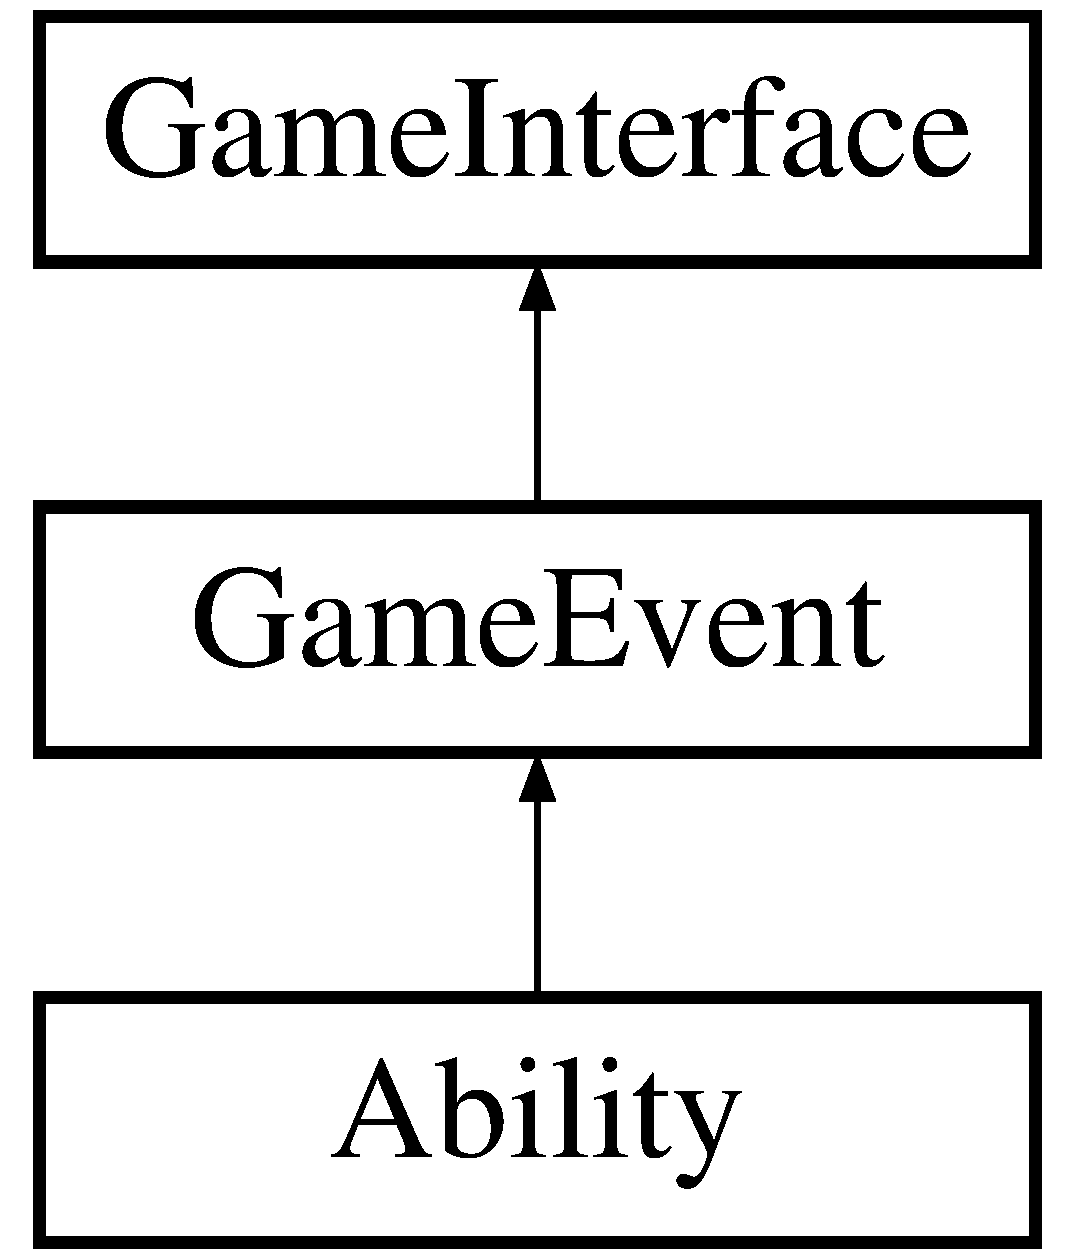
\includegraphics[height=3.000000cm]{class_ability}
\end{center}
\end{figure}
\subsection*{Public Member Functions}
\begin{DoxyCompactItemize}
\item 
virtual void \hyperlink{class_ability_a1a960040b98f8632a675ad184ead84b3}{notify} ()
\item 
virtual void \hyperlink{class_ability_af5d8c9005cc4b4b2a8f650cc10529924}{operator()} ()
\end{DoxyCompactItemize}
\subsection*{Additional Inherited Members}


\subsection{Detailed Description}
A generic base class that will usually serve as the return type for any complex action that a character can perform, such as using magic attacks or healing 

Definition at line 21 of file Ability.\-h.



\subsection{Member Function Documentation}
\hypertarget{class_ability_a1a960040b98f8632a675ad184ead84b3}{\index{Ability@{Ability}!notify@{notify}}
\index{notify@{notify}!Ability@{Ability}}
\subsubsection[{notify}]{\setlength{\rightskip}{0pt plus 5cm}void Ability\-::notify (
\begin{DoxyParamCaption}
{}
\end{DoxyParamCaption}
)\hspace{0.3cm}{\ttfamily [virtual]}}}\label{class_ability_a1a960040b98f8632a675ad184ead84b3}


Reimplemented from \hyperlink{class_game_event_a2effcb2226837b007cfb27defbd5658e}{Game\-Event}.



Definition at line 11 of file Ability.\-cpp.

\hypertarget{class_ability_af5d8c9005cc4b4b2a8f650cc10529924}{\index{Ability@{Ability}!operator()@{operator()}}
\index{operator()@{operator()}!Ability@{Ability}}
\subsubsection[{operator()}]{\setlength{\rightskip}{0pt plus 5cm}void Ability\-::operator() (
\begin{DoxyParamCaption}
{}
\end{DoxyParamCaption}
)\hspace{0.3cm}{\ttfamily [virtual]}}}\label{class_ability_af5d8c9005cc4b4b2a8f650cc10529924}
An implementing class can define a default function by overloading its () operator 

Reimplemented from \hyperlink{class_game_event_a0d21300957e0a82e4fcfdd7dd8ad9449}{Game\-Event}.



Definition at line 15 of file Ability.\-cpp.



The documentation for this class was generated from the following files\-:\begin{DoxyCompactItemize}
\item 
/\-Volumes/\-O\-S X H\-D\-D/\-Users/\-Adam/\-Developer/\-Sprite\-Fight/\-World/\hyperlink{_ability_8h}{Ability.\-h}\item 
/\-Volumes/\-O\-S X H\-D\-D/\-Users/\-Adam/\-Developer/\-Sprite\-Fight/\-World/\hyperlink{_ability_8cpp}{Ability.\-cpp}\end{DoxyCompactItemize}

\hypertarget{struct_asset_file}{\section{Asset\-File Struct Reference}
\label{struct_asset_file}\index{Asset\-File@{Asset\-File}}
}


{\ttfamily \#include $<$Asset\-File\-I\-O.\-h$>$}

\subsection*{Public Member Functions}
\begin{DoxyCompactItemize}
\item 
\hyperlink{struct_asset_file_a138aff39a7ba0752bc64f917bde5cfe7}{Asset\-File} ()
\item 
\hyperlink{struct_asset_file_a80c0a491cfcf6ebfb5974d450a6cf3c7}{Asset\-File} (string \hyperlink{struct_asset_file_a6d2915fb2e781c162752036028bf9b32}{file\-Name}, string \hyperlink{struct_asset_file_a25c3567f452df062ea7dcee79c0aefde}{file\-Path}, \hyperlink{_asset_file_i_o_8h_a72d924d1cb8e1544b6d5198e98d52ca9}{Asset\-Type} \hyperlink{struct_asset_file_ad154debe8690c8bd1c29d091cabea4e7}{type}, \hyperlink{_character_data_8h_a55ecd4f2ec2ebfe8d5b0163e4ac2a967}{Colors} \hyperlink{struct_asset_file_a9665f3c7769b8cee2106d718de7c297c}{color})
\item 
\hyperlink{struct_asset_file_ac60659d896166a29083a443f38f1ef05}{Asset\-File} (const \hyperlink{struct_asset_file}{Asset\-File} \&other)
\item 
\hyperlink{struct_asset_file_add1d27fe2e94cda56bf6681ba5fd4ffc}{Asset\-File} (const string \&existing\-Filename)
\item 
\hyperlink{struct_asset_file_a7f4c4b962f0fe6fd880fcd22138ccde0}{Asset\-File} (\hyperlink{class_fast_rand}{Fast\-Rand}$<$ int $>$ randm)
\item 
\hyperlink{struct_asset_file_a067d33d121eef312ba85bd918dc4ac79}{$\sim$\-Asset\-File} ()
\item 
\hyperlink{struct_asset_file}{Asset\-File} \& \hyperlink{struct_asset_file_abc472db3c90c0db73f61da6df919c38b}{operator=} (const \hyperlink{struct_asset_file}{Asset\-File} \&rhs)
\item 
\hyperlink{struct_asset_file}{Asset\-File} \& \hyperlink{struct_asset_file_a58917e9118b1e2363ef69d174063fd02}{operator=} (const string \&str)
\end{DoxyCompactItemize}
\subsection*{Public Attributes}
\begin{DoxyCompactItemize}
\item 
string \hyperlink{struct_asset_file_a6d2915fb2e781c162752036028bf9b32}{file\-Name}
\item 
\hyperlink{_asset_file_i_o_8h_a72d924d1cb8e1544b6d5198e98d52ca9}{Asset\-Type} \hyperlink{struct_asset_file_ad154debe8690c8bd1c29d091cabea4e7}{type}
\item 
\hyperlink{_character_data_8h_a55ecd4f2ec2ebfe8d5b0163e4ac2a967}{Colors} \hyperlink{struct_asset_file_a9665f3c7769b8cee2106d718de7c297c}{color}
\end{DoxyCompactItemize}
\subsection*{Static Public Attributes}
\begin{DoxyCompactItemize}
\item 
static vector$<$ \hyperlink{struct_asset_file}{Asset\-File} $>$ $\ast$ \hyperlink{struct_asset_file_a7482e097719d1baa3a15fc3a5a00e15e}{asteroid\-Image\-Filenames}
\item 
static vector$<$ \hyperlink{struct_asset_file}{Asset\-File} $>$ $\ast$ \hyperlink{struct_asset_file_a54cd19685e8f404021aeef79eb775430}{background\-Image\-Filenames}
\item 
static vector$<$ \hyperlink{struct_asset_file}{Asset\-File} $>$ $\ast$ \hyperlink{struct_asset_file_a71a63898ce62bf0afc9fc1e8736cfb1d}{explosion\-Image\-Filenames}
\item 
static vector$<$ \hyperlink{struct_asset_file}{Asset\-File} $>$ $\ast$ \hyperlink{struct_asset_file_afcf268447c77710c71d5503668e0afb7}{powerup\-Image\-Filenames}
\item 
static vector$<$ \hyperlink{struct_asset_file}{Asset\-File} $>$ $\ast$ \hyperlink{struct_asset_file_aa4c45964db96750b68dc082ccbd6adb3}{projectile\-Image\-Filenames}
\item 
static vector$<$ \hyperlink{struct_asset_file}{Asset\-File} $>$ $\ast$ \hyperlink{struct_asset_file_a190e00509710ab08fa4effe17ef443f0}{shield\-Image\-Filenames}
\item 
static vector$<$ \hyperlink{struct_asset_file}{Asset\-File} $>$ $\ast$ \hyperlink{struct_asset_file_a2e2753d8110ad1c4726f724e15f5b831}{player\-Ship\-Image\-Filenames}
\item 
static vector$<$ \hyperlink{struct_asset_file}{Asset\-File} $>$ $\ast$ \hyperlink{struct_asset_file_a792cd746ec7903ca9d34a094627bc947}{enemy\-Ship\-Image\-Filenames}
\item 
static vector$<$ \hyperlink{struct_asset_file}{Asset\-File} $>$ $\ast$ \hyperlink{struct_asset_file_a372beb61728cbc13001766c79ab1ee70}{ship\-Damage\-Image\-Filenames}
\item 
static vector$<$ \hyperlink{struct_asset_file}{Asset\-File} $>$ $\ast$ \hyperlink{struct_asset_file_a453cc790da71efe1ad15a45d1a3cde40}{U\-I\-Image\-Filenames}
\item 
static vector$<$ vector\\*
$<$ \hyperlink{struct_asset_file}{Asset\-File} $>$ $\ast$ $>$ $\ast$ \hyperlink{struct_asset_file_a9bd02c38dcc2dc973d65b92c80d35570}{all\-Asset\-Files}
\end{DoxyCompactItemize}
\subsection*{Protected Attributes}
\begin{DoxyCompactItemize}
\item 
string \hyperlink{struct_asset_file_a25c3567f452df062ea7dcee79c0aefde}{file\-Path}
\end{DoxyCompactItemize}
\subsection*{Friends}
\begin{DoxyCompactItemize}
\item 
class \hyperlink{struct_asset_file_a27c2caf7607df43b8f078b2e3d37133e}{Asset\-File\-I\-O}
\end{DoxyCompactItemize}


\subsection{Detailed Description}


Definition at line 47 of file Asset\-File\-I\-O.\-h.



\subsection{Constructor \& Destructor Documentation}
\hypertarget{struct_asset_file_a138aff39a7ba0752bc64f917bde5cfe7}{\index{Asset\-File@{Asset\-File}!Asset\-File@{Asset\-File}}
\index{Asset\-File@{Asset\-File}!AssetFile@{Asset\-File}}
\subsubsection[{Asset\-File}]{\setlength{\rightskip}{0pt plus 5cm}Asset\-File\-::\-Asset\-File (
\begin{DoxyParamCaption}
{}
\end{DoxyParamCaption}
)\hspace{0.3cm}{\ttfamily [inline]}}}\label{struct_asset_file_a138aff39a7ba0752bc64f917bde5cfe7}


Definition at line 75 of file Asset\-File\-I\-O.\-h.

\hypertarget{struct_asset_file_a80c0a491cfcf6ebfb5974d450a6cf3c7}{\index{Asset\-File@{Asset\-File}!Asset\-File@{Asset\-File}}
\index{Asset\-File@{Asset\-File}!AssetFile@{Asset\-File}}
\subsubsection[{Asset\-File}]{\setlength{\rightskip}{0pt plus 5cm}Asset\-File\-::\-Asset\-File (
\begin{DoxyParamCaption}
\item[{string}]{file\-Name, }
\item[{string}]{file\-Path, }
\item[{{\bf Asset\-Type}}]{type, }
\item[{{\bf Colors}}]{color}
\end{DoxyParamCaption}
)\hspace{0.3cm}{\ttfamily [inline]}}}\label{struct_asset_file_a80c0a491cfcf6ebfb5974d450a6cf3c7}


Definition at line 78 of file Asset\-File\-I\-O.\-h.

\hypertarget{struct_asset_file_ac60659d896166a29083a443f38f1ef05}{\index{Asset\-File@{Asset\-File}!Asset\-File@{Asset\-File}}
\index{Asset\-File@{Asset\-File}!AssetFile@{Asset\-File}}
\subsubsection[{Asset\-File}]{\setlength{\rightskip}{0pt plus 5cm}Asset\-File\-::\-Asset\-File (
\begin{DoxyParamCaption}
\item[{const {\bf Asset\-File} \&}]{other}
\end{DoxyParamCaption}
)\hspace{0.3cm}{\ttfamily [inline]}}}\label{struct_asset_file_ac60659d896166a29083a443f38f1ef05}


Definition at line 81 of file Asset\-File\-I\-O.\-h.

\hypertarget{struct_asset_file_add1d27fe2e94cda56bf6681ba5fd4ffc}{\index{Asset\-File@{Asset\-File}!Asset\-File@{Asset\-File}}
\index{Asset\-File@{Asset\-File}!AssetFile@{Asset\-File}}
\subsubsection[{Asset\-File}]{\setlength{\rightskip}{0pt plus 5cm}Asset\-File\-::\-Asset\-File (
\begin{DoxyParamCaption}
\item[{const string \&}]{existing\-Filename}
\end{DoxyParamCaption}
)}}\label{struct_asset_file_add1d27fe2e94cda56bf6681ba5fd4ffc}


Definition at line 103 of file Asset\-File\-I\-O.\-cpp.

\hypertarget{struct_asset_file_a7f4c4b962f0fe6fd880fcd22138ccde0}{\index{Asset\-File@{Asset\-File}!Asset\-File@{Asset\-File}}
\index{Asset\-File@{Asset\-File}!AssetFile@{Asset\-File}}
\subsubsection[{Asset\-File}]{\setlength{\rightskip}{0pt plus 5cm}Asset\-File\-::\-Asset\-File (
\begin{DoxyParamCaption}
\item[{{\bf Fast\-Rand}$<$ int $>$}]{randm}
\end{DoxyParamCaption}
)}}\label{struct_asset_file_a7f4c4b962f0fe6fd880fcd22138ccde0}


Definition at line 120 of file Asset\-File\-I\-O.\-cpp.

\hypertarget{struct_asset_file_a067d33d121eef312ba85bd918dc4ac79}{\index{Asset\-File@{Asset\-File}!$\sim$\-Asset\-File@{$\sim$\-Asset\-File}}
\index{$\sim$\-Asset\-File@{$\sim$\-Asset\-File}!AssetFile@{Asset\-File}}
\subsubsection[{$\sim$\-Asset\-File}]{\setlength{\rightskip}{0pt plus 5cm}Asset\-File\-::$\sim$\-Asset\-File (
\begin{DoxyParamCaption}
{}
\end{DoxyParamCaption}
)\hspace{0.3cm}{\ttfamily [inline]}}}\label{struct_asset_file_a067d33d121eef312ba85bd918dc4ac79}


Definition at line 88 of file Asset\-File\-I\-O.\-h.



\subsection{Member Function Documentation}
\hypertarget{struct_asset_file_abc472db3c90c0db73f61da6df919c38b}{\index{Asset\-File@{Asset\-File}!operator=@{operator=}}
\index{operator=@{operator=}!AssetFile@{Asset\-File}}
\subsubsection[{operator=}]{\setlength{\rightskip}{0pt plus 5cm}{\bf Asset\-File} \& Asset\-File\-::operator= (
\begin{DoxyParamCaption}
\item[{const {\bf Asset\-File} \&}]{rhs}
\end{DoxyParamCaption}
)}}\label{struct_asset_file_abc472db3c90c0db73f61da6df919c38b}


Definition at line 129 of file Asset\-File\-I\-O.\-cpp.

\hypertarget{struct_asset_file_a58917e9118b1e2363ef69d174063fd02}{\index{Asset\-File@{Asset\-File}!operator=@{operator=}}
\index{operator=@{operator=}!AssetFile@{Asset\-File}}
\subsubsection[{operator=}]{\setlength{\rightskip}{0pt plus 5cm}{\bf Asset\-File} \& Asset\-File\-::operator= (
\begin{DoxyParamCaption}
\item[{const string \&}]{str}
\end{DoxyParamCaption}
)}}\label{struct_asset_file_a58917e9118b1e2363ef69d174063fd02}


Definition at line 140 of file Asset\-File\-I\-O.\-cpp.



\subsection{Friends And Related Function Documentation}
\hypertarget{struct_asset_file_a27c2caf7607df43b8f078b2e3d37133e}{\index{Asset\-File@{Asset\-File}!Asset\-File\-I\-O@{Asset\-File\-I\-O}}
\index{Asset\-File\-I\-O@{Asset\-File\-I\-O}!AssetFile@{Asset\-File}}
\subsubsection[{Asset\-File\-I\-O}]{\setlength{\rightskip}{0pt plus 5cm}friend class {\bf Asset\-File\-I\-O}\hspace{0.3cm}{\ttfamily [friend]}}}\label{struct_asset_file_a27c2caf7607df43b8f078b2e3d37133e}


Definition at line 51 of file Asset\-File\-I\-O.\-h.



\subsection{Member Data Documentation}
\hypertarget{struct_asset_file_a9bd02c38dcc2dc973d65b92c80d35570}{\index{Asset\-File@{Asset\-File}!all\-Asset\-Files@{all\-Asset\-Files}}
\index{all\-Asset\-Files@{all\-Asset\-Files}!AssetFile@{Asset\-File}}
\subsubsection[{all\-Asset\-Files}]{\setlength{\rightskip}{0pt plus 5cm}vector$<$ vector$<$ {\bf Asset\-File} $>$ $\ast$ $>$ $\ast$ Asset\-File\-::all\-Asset\-Files\hspace{0.3cm}{\ttfamily [static]}}}\label{struct_asset_file_a9bd02c38dcc2dc973d65b92c80d35570}
{\bfseries Initial value\-:}
\begin{DoxyCode}
= \textcolor{keyword}{new} vector< vector<AssetFile> * > \{
    \hyperlink{struct_asset_file_a7482e097719d1baa3a15fc3a5a00e15e}{asteroidImageFilenames},
    \hyperlink{struct_asset_file_a54cd19685e8f404021aeef79eb775430}{backgroundImageFilenames},
    \hyperlink{struct_asset_file_a71a63898ce62bf0afc9fc1e8736cfb1d}{explosionImageFilenames},
    \hyperlink{struct_asset_file_afcf268447c77710c71d5503668e0afb7}{powerupImageFilenames},
    \hyperlink{struct_asset_file_aa4c45964db96750b68dc082ccbd6adb3}{projectileImageFilenames},
    \hyperlink{struct_asset_file_a190e00509710ab08fa4effe17ef443f0}{shieldImageFilenames},
    \hyperlink{struct_asset_file_a2e2753d8110ad1c4726f724e15f5b831}{playerShipImageFilenames},
    \hyperlink{struct_asset_file_a792cd746ec7903ca9d34a094627bc947}{enemyShipImageFilenames},
    \hyperlink{struct_asset_file_a372beb61728cbc13001766c79ab1ee70}{shipDamageImageFilenames},
    \hyperlink{struct_asset_file_a453cc790da71efe1ad15a45d1a3cde40}{UIImageFilenames}
    
\}
\end{DoxyCode}


Definition at line 68 of file Asset\-File\-I\-O.\-h.

\hypertarget{struct_asset_file_a7482e097719d1baa3a15fc3a5a00e15e}{\index{Asset\-File@{Asset\-File}!asteroid\-Image\-Filenames@{asteroid\-Image\-Filenames}}
\index{asteroid\-Image\-Filenames@{asteroid\-Image\-Filenames}!AssetFile@{Asset\-File}}
\subsubsection[{asteroid\-Image\-Filenames}]{\setlength{\rightskip}{0pt plus 5cm}vector$<$ {\bf Asset\-File} $>$ $\ast$ Asset\-File\-::asteroid\-Image\-Filenames\hspace{0.3cm}{\ttfamily [static]}}}\label{struct_asset_file_a7482e097719d1baa3a15fc3a5a00e15e}
{\bfseries Initial value\-:}
\begin{DoxyCode}
= \textcolor{keyword}{new} vector<AssetFile> \{
    \{\textcolor{stringliteral}{"Asteroid0\_Brown.png"}, \textcolor{stringliteral}{"/Assets/Asteroids/Asteroid0\_Brown.png"}, 
      \hyperlink{_asset_file_i_o_8h_a72d924d1cb8e1544b6d5198e98d52ca9acd76adfdb0f7227ec28f6dc8d0cb3221}{AssetType::asteroid}, \hyperlink{_character_data_8h_a55ecd4f2ec2ebfe8d5b0163e4ac2a967a6ff47afa5dc7daa42cc705a03fca8a9b}{Colors::brown}\},
    \{\textcolor{stringliteral}{"Asteroid0\_Gray.png"},  \textcolor{stringliteral}{"/Assets/Asteroids/Asteroid0\_Gray.png"},  
      \hyperlink{_asset_file_i_o_8h_a72d924d1cb8e1544b6d5198e98d52ca9acd76adfdb0f7227ec28f6dc8d0cb3221}{AssetType::asteroid}, \hyperlink{_character_data_8h_a55ecd4f2ec2ebfe8d5b0163e4ac2a967a6ff47afa5dc7daa42cc705a03fca8a9b}{Colors::brown}\}
\}
\end{DoxyCode}


Definition at line 57 of file Asset\-File\-I\-O.\-h.

\hypertarget{struct_asset_file_a54cd19685e8f404021aeef79eb775430}{\index{Asset\-File@{Asset\-File}!background\-Image\-Filenames@{background\-Image\-Filenames}}
\index{background\-Image\-Filenames@{background\-Image\-Filenames}!AssetFile@{Asset\-File}}
\subsubsection[{background\-Image\-Filenames}]{\setlength{\rightskip}{0pt plus 5cm}vector$<$ {\bf Asset\-File} $>$ $\ast$ Asset\-File\-::background\-Image\-Filenames\hspace{0.3cm}{\ttfamily [static]}}}\label{struct_asset_file_a54cd19685e8f404021aeef79eb775430}
{\bfseries Initial value\-:}
\begin{DoxyCode}
= \textcolor{keyword}{new} vector<AssetFile> \{
    \{\textcolor{stringliteral}{"Space 0.png"}, \textcolor{stringliteral}{"/Assets/Backgrounds/Space 0.png"}, \hyperlink{_asset_file_i_o_8h_a72d924d1cb8e1544b6d5198e98d52ca9ad229bbf31eaeebc7c88897732d8b932d}{AssetType::background}, 
      \hyperlink{_character_data_8h_a55ecd4f2ec2ebfe8d5b0163e4ac2a967a16875aa2b5eed3e388dcceaa36f56214}{Colors::various}\}
\}
\end{DoxyCode}


Definition at line 58 of file Asset\-File\-I\-O.\-h.

\hypertarget{struct_asset_file_a9665f3c7769b8cee2106d718de7c297c}{\index{Asset\-File@{Asset\-File}!color@{color}}
\index{color@{color}!AssetFile@{Asset\-File}}
\subsubsection[{color}]{\setlength{\rightskip}{0pt plus 5cm}{\bf Colors} Asset\-File\-::color}}\label{struct_asset_file_a9665f3c7769b8cee2106d718de7c297c}


Definition at line 72 of file Asset\-File\-I\-O.\-h.

\hypertarget{struct_asset_file_a792cd746ec7903ca9d34a094627bc947}{\index{Asset\-File@{Asset\-File}!enemy\-Ship\-Image\-Filenames@{enemy\-Ship\-Image\-Filenames}}
\index{enemy\-Ship\-Image\-Filenames@{enemy\-Ship\-Image\-Filenames}!AssetFile@{Asset\-File}}
\subsubsection[{enemy\-Ship\-Image\-Filenames}]{\setlength{\rightskip}{0pt plus 5cm}vector$<$ {\bf Asset\-File} $>$ $\ast$ Asset\-File\-::enemy\-Ship\-Image\-Filenames\hspace{0.3cm}{\ttfamily [static]}}}\label{struct_asset_file_a792cd746ec7903ca9d34a094627bc947}
{\bfseries Initial value\-:}
\begin{DoxyCode}
= \textcolor{keyword}{new} vector<AssetFile> \{
    \{\textcolor{stringliteral}{"Enemy\_Ship0\_Blue.png"},   \textcolor{stringliteral}{"/Assets/Ships/Enemy\_Ship0\_Blue.png"},    
      \hyperlink{_asset_file_i_o_8h_a72d924d1cb8e1544b6d5198e98d52ca9a7a484b4c7c5ba2d013a34d7b28636ade}{AssetType::enemyShip}, \hyperlink{_character_data_8h_a55ecd4f2ec2ebfe8d5b0163e4ac2a967a48d6215903dff56238e52e8891380c8f}{Colors::blue}\},
    \{\textcolor{stringliteral}{"Enemy\_Ship0\_Orange.png"}, \textcolor{stringliteral}{"/Assets/Ships/Enemy\_Ship0\_Orange.png"},  
      \hyperlink{_asset_file_i_o_8h_a72d924d1cb8e1544b6d5198e98d52ca9a7a484b4c7c5ba2d013a34d7b28636ade}{AssetType::enemyShip}, \hyperlink{_character_data_8h_a55ecd4f2ec2ebfe8d5b0163e4ac2a967afe01d67a002dfa0f3ac084298142eccd}{Colors::orange}\},
    \{\textcolor{stringliteral}{"Enemy\_Ship2\_Blue.png"},   \textcolor{stringliteral}{"/Assets/Ships/Enemy\_Ship2\_Blue.png"},    
      \hyperlink{_asset_file_i_o_8h_a72d924d1cb8e1544b6d5198e98d52ca9a7a484b4c7c5ba2d013a34d7b28636ade}{AssetType::enemyShip}, \hyperlink{_character_data_8h_a55ecd4f2ec2ebfe8d5b0163e4ac2a967a48d6215903dff56238e52e8891380c8f}{Colors::blue}\},
    \{\textcolor{stringliteral}{"Enemy\_Ship2\_Green.png"},  \textcolor{stringliteral}{"/Assets/Ships/Enemy\_Ship2\_Green.png"},   
      \hyperlink{_asset_file_i_o_8h_a72d924d1cb8e1544b6d5198e98d52ca9a7a484b4c7c5ba2d013a34d7b28636ade}{AssetType::enemyShip}, \hyperlink{_character_data_8h_a55ecd4f2ec2ebfe8d5b0163e4ac2a967a9f27410725ab8cc8854a2769c7a516b8}{Colors::green}\}
\}
\end{DoxyCode}


Definition at line 64 of file Asset\-File\-I\-O.\-h.

\hypertarget{struct_asset_file_a71a63898ce62bf0afc9fc1e8736cfb1d}{\index{Asset\-File@{Asset\-File}!explosion\-Image\-Filenames@{explosion\-Image\-Filenames}}
\index{explosion\-Image\-Filenames@{explosion\-Image\-Filenames}!AssetFile@{Asset\-File}}
\subsubsection[{explosion\-Image\-Filenames}]{\setlength{\rightskip}{0pt plus 5cm}vector$<$ {\bf Asset\-File} $>$ $\ast$ Asset\-File\-::explosion\-Image\-Filenames\hspace{0.3cm}{\ttfamily [static]}}}\label{struct_asset_file_a71a63898ce62bf0afc9fc1e8736cfb1d}
{\bfseries Initial value\-:}
\begin{DoxyCode}
= \textcolor{keyword}{new} vector<AssetFile> \{
    \{\textcolor{stringliteral}{"Explosion0\_Blue.png"},     \textcolor{stringliteral}{"/Assets/Explosions/Explosion0\_Blue.png"},       
      \hyperlink{_asset_file_i_o_8h_a72d924d1cb8e1544b6d5198e98d52ca9a0f90cac94bfd7222b85c4114d122c5ac}{AssetType::explosion}, \hyperlink{_character_data_8h_a55ecd4f2ec2ebfe8d5b0163e4ac2a967a48d6215903dff56238e52e8891380c8f}{Colors::blue}\},
    \{\textcolor{stringliteral}{"Explosion0\_Green.png"},    \textcolor{stringliteral}{"/Assets/Explosions/Explosion0\_Green.png"},      
      \hyperlink{_asset_file_i_o_8h_a72d924d1cb8e1544b6d5198e98d52ca9a0f90cac94bfd7222b85c4114d122c5ac}{AssetType::explosion}, \hyperlink{_character_data_8h_a55ecd4f2ec2ebfe8d5b0163e4ac2a967a9f27410725ab8cc8854a2769c7a516b8}{Colors::green}\},
    \{\textcolor{stringliteral}{"Explosion0\_Red.png"},      \textcolor{stringliteral}{"/Assets/Explosions/Explosion0\_Red.png"},        
      \hyperlink{_asset_file_i_o_8h_a72d924d1cb8e1544b6d5198e98d52ca9a0f90cac94bfd7222b85c4114d122c5ac}{AssetType::explosion}, \hyperlink{_character_data_8h_a55ecd4f2ec2ebfe8d5b0163e4ac2a967abda9643ac6601722a28f238714274da4}{Colors::red}\}
\}
\end{DoxyCode}


Definition at line 59 of file Asset\-File\-I\-O.\-h.

\hypertarget{struct_asset_file_a6d2915fb2e781c162752036028bf9b32}{\index{Asset\-File@{Asset\-File}!file\-Name@{file\-Name}}
\index{file\-Name@{file\-Name}!AssetFile@{Asset\-File}}
\subsubsection[{file\-Name}]{\setlength{\rightskip}{0pt plus 5cm}string Asset\-File\-::file\-Name}}\label{struct_asset_file_a6d2915fb2e781c162752036028bf9b32}


Definition at line 70 of file Asset\-File\-I\-O.\-h.

\hypertarget{struct_asset_file_a25c3567f452df062ea7dcee79c0aefde}{\index{Asset\-File@{Asset\-File}!file\-Path@{file\-Path}}
\index{file\-Path@{file\-Path}!AssetFile@{Asset\-File}}
\subsubsection[{file\-Path}]{\setlength{\rightskip}{0pt plus 5cm}string Asset\-File\-::file\-Path\hspace{0.3cm}{\ttfamily [protected]}}}\label{struct_asset_file_a25c3567f452df062ea7dcee79c0aefde}


Definition at line 53 of file Asset\-File\-I\-O.\-h.

\hypertarget{struct_asset_file_a2e2753d8110ad1c4726f724e15f5b831}{\index{Asset\-File@{Asset\-File}!player\-Ship\-Image\-Filenames@{player\-Ship\-Image\-Filenames}}
\index{player\-Ship\-Image\-Filenames@{player\-Ship\-Image\-Filenames}!AssetFile@{Asset\-File}}
\subsubsection[{player\-Ship\-Image\-Filenames}]{\setlength{\rightskip}{0pt plus 5cm}vector$<$ {\bf Asset\-File} $>$ $\ast$ Asset\-File\-::player\-Ship\-Image\-Filenames\hspace{0.3cm}{\ttfamily [static]}}}\label{struct_asset_file_a2e2753d8110ad1c4726f724e15f5b831}
{\bfseries Initial value\-:}
\begin{DoxyCode}
= \textcolor{keyword}{new} vector<AssetFile> \{
    \{\textcolor{stringliteral}{"Saucer\_Red.png"},  \textcolor{stringliteral}{"/Assets/Ships/Saucer\_Red.png"},  \hyperlink{_asset_file_i_o_8h_a72d924d1cb8e1544b6d5198e98d52ca9a4c08b14797b28df331a55e03fff1b2e6}{AssetType::playerShip}, 
      \hyperlink{_character_data_8h_a55ecd4f2ec2ebfe8d5b0163e4ac2a967abda9643ac6601722a28f238714274da4}{Colors::red}\},
    \{\textcolor{stringliteral}{"Ship0\_Blue.png"},  \textcolor{stringliteral}{"/Assets/Ships/Ship0\_Blue.png"},  \hyperlink{_asset_file_i_o_8h_a72d924d1cb8e1544b6d5198e98d52ca9a4c08b14797b28df331a55e03fff1b2e6}{AssetType::playerShip}, 
      \hyperlink{_character_data_8h_a55ecd4f2ec2ebfe8d5b0163e4ac2a967a48d6215903dff56238e52e8891380c8f}{Colors::blue}\},
    \{\textcolor{stringliteral}{"Ship0\_Red.png"},   \textcolor{stringliteral}{"/Assets/Ships/Ship0\_Red.png"},   \hyperlink{_asset_file_i_o_8h_a72d924d1cb8e1544b6d5198e98d52ca9a4c08b14797b28df331a55e03fff1b2e6}{AssetType::playerShip}, 
      \hyperlink{_character_data_8h_a55ecd4f2ec2ebfe8d5b0163e4ac2a967abda9643ac6601722a28f238714274da4}{Colors::red}\},
    \{\textcolor{stringliteral}{"Ship1\_Green.png"}, \textcolor{stringliteral}{"/Assets/Ships/Ship1\_Green.png"}, \hyperlink{_asset_file_i_o_8h_a72d924d1cb8e1544b6d5198e98d52ca9a4c08b14797b28df331a55e03fff1b2e6}{AssetType::playerShip}, 
      \hyperlink{_character_data_8h_a55ecd4f2ec2ebfe8d5b0163e4ac2a967a9f27410725ab8cc8854a2769c7a516b8}{Colors::green}\},
    \{\textcolor{stringliteral}{"Ship2\_Blue.png"},  \textcolor{stringliteral}{"/Assets/Ships/Ship2\_Blue.png"},  \hyperlink{_asset_file_i_o_8h_a72d924d1cb8e1544b6d5198e98d52ca9a4c08b14797b28df331a55e03fff1b2e6}{AssetType::playerShip}, 
      \hyperlink{_character_data_8h_a55ecd4f2ec2ebfe8d5b0163e4ac2a967a48d6215903dff56238e52e8891380c8f}{Colors::blue}\}

\}
\end{DoxyCode}


Definition at line 63 of file Asset\-File\-I\-O.\-h.

\hypertarget{struct_asset_file_afcf268447c77710c71d5503668e0afb7}{\index{Asset\-File@{Asset\-File}!powerup\-Image\-Filenames@{powerup\-Image\-Filenames}}
\index{powerup\-Image\-Filenames@{powerup\-Image\-Filenames}!AssetFile@{Asset\-File}}
\subsubsection[{powerup\-Image\-Filenames}]{\setlength{\rightskip}{0pt plus 5cm}vector$<$ {\bf Asset\-File} $>$ $\ast$ Asset\-File\-::powerup\-Image\-Filenames\hspace{0.3cm}{\ttfamily [static]}}}\label{struct_asset_file_afcf268447c77710c71d5503668e0afb7}
{\bfseries Initial value\-:}
\begin{DoxyCode}
= \textcolor{keyword}{new} vector<AssetFile> \{

    \{\textcolor{stringliteral}{"EngineThrust0.png"}, \textcolor{stringliteral}{"/Assets/Powerups/EngineThrust0.png"}, 
      \hyperlink{_asset_file_i_o_8h_a72d924d1cb8e1544b6d5198e98d52ca9af287c6beccb1f257def546ad6acdd9e4}{AssetType::powerup}, \hyperlink{_character_data_8h_a55ecd4f2ec2ebfe8d5b0163e4ac2a967a5e96bf62b9b2c18fdb65564b4a18fd1f}{Colors::transparent}\},
    \{\textcolor{stringliteral}{"Bolt\_Gold.png"},     \textcolor{stringliteral}{"/Assets/Powerups/Bolt\_Gold.png"},     
      \hyperlink{_asset_file_i_o_8h_a72d924d1cb8e1544b6d5198e98d52ca9af287c6beccb1f257def546ad6acdd9e4}{AssetType::powerup}, \hyperlink{_character_data_8h_a55ecd4f2ec2ebfe8d5b0163e4ac2a967ae07e81c20cf5935f5225765f0af81755}{Colors::gold}\},
    \{\textcolor{stringliteral}{"Pill\_Blue.png"},     \textcolor{stringliteral}{"/Assets/Powerups/Pill\_Blue.png"},     
      \hyperlink{_asset_file_i_o_8h_a72d924d1cb8e1544b6d5198e98d52ca9af287c6beccb1f257def546ad6acdd9e4}{AssetType::powerup}, \hyperlink{_character_data_8h_a55ecd4f2ec2ebfe8d5b0163e4ac2a967a48d6215903dff56238e52e8891380c8f}{Colors::blue}\},
    \{\textcolor{stringliteral}{"Pill\_Green.png"},    \textcolor{stringliteral}{"/Assets/Powerups/Pill\_Green.png"},    
      \hyperlink{_asset_file_i_o_8h_a72d924d1cb8e1544b6d5198e98d52ca9af287c6beccb1f257def546ad6acdd9e4}{AssetType::powerup}, \hyperlink{_character_data_8h_a55ecd4f2ec2ebfe8d5b0163e4ac2a967a48d6215903dff56238e52e8891380c8f}{Colors::blue}\},
    \{\textcolor{stringliteral}{"Shield\_Silver.png"}, \textcolor{stringliteral}{"/Assets/Powerups/Shield\_Silver.png"}, 
      \hyperlink{_asset_file_i_o_8h_a72d924d1cb8e1544b6d5198e98d52ca9af287c6beccb1f257def546ad6acdd9e4}{AssetType::powerup}, \hyperlink{_character_data_8h_a55ecd4f2ec2ebfe8d5b0163e4ac2a967a97f014516561ef487ec368d6158eb3f4}{Colors::silver}\}
\}
\end{DoxyCode}


Definition at line 60 of file Asset\-File\-I\-O.\-h.

\hypertarget{struct_asset_file_aa4c45964db96750b68dc082ccbd6adb3}{\index{Asset\-File@{Asset\-File}!projectile\-Image\-Filenames@{projectile\-Image\-Filenames}}
\index{projectile\-Image\-Filenames@{projectile\-Image\-Filenames}!AssetFile@{Asset\-File}}
\subsubsection[{projectile\-Image\-Filenames}]{\setlength{\rightskip}{0pt plus 5cm}vector$<$ {\bf Asset\-File} $>$ $\ast$ Asset\-File\-::projectile\-Image\-Filenames\hspace{0.3cm}{\ttfamily [static]}}}\label{struct_asset_file_aa4c45964db96750b68dc082ccbd6adb3}
{\bfseries Initial value\-:}
\begin{DoxyCode}
= \textcolor{keyword}{new} vector<AssetFile> \{
    \{\textcolor{stringliteral}{"LaserBlast0\_Green.png"},   \textcolor{stringliteral}{"/Assets/Projectiles/LaserBlast0\_Green.png"},    
      \hyperlink{_asset_file_i_o_8h_a72d924d1cb8e1544b6d5198e98d52ca9abdb3aea80363d8d4bded1ce9f3cdadf2}{AssetType::projectile}, \hyperlink{_character_data_8h_a55ecd4f2ec2ebfe8d5b0163e4ac2a967a9f27410725ab8cc8854a2769c7a516b8}{Colors::green}\},
    \{\textcolor{stringliteral}{"LaserBlast0\_Red.png"},     \textcolor{stringliteral}{"/Assets/Projectiles/LaserBlast0\_Red.png"},      
      \hyperlink{_asset_file_i_o_8h_a72d924d1cb8e1544b6d5198e98d52ca9abdb3aea80363d8d4bded1ce9f3cdadf2}{AssetType::projectile}, \hyperlink{_character_data_8h_a55ecd4f2ec2ebfe8d5b0163e4ac2a967abda9643ac6601722a28f238714274da4}{Colors::red}\},
    \{\textcolor{stringliteral}{"LaserBlast1\_Blue.png"},    \textcolor{stringliteral}{"/Assets/Projectiles/LaserBlast1\_Blue.png"},     
      \hyperlink{_asset_file_i_o_8h_a72d924d1cb8e1544b6d5198e98d52ca9abdb3aea80363d8d4bded1ce9f3cdadf2}{AssetType::projectile}, \hyperlink{_character_data_8h_a55ecd4f2ec2ebfe8d5b0163e4ac2a967a48d6215903dff56238e52e8891380c8f}{Colors::blue}\},
    \{\textcolor{stringliteral}{"LaserBlast1\_Green.png"},   \textcolor{stringliteral}{"/Assets/Projectiles/LaserBlast1\_Green.png"},    
      \hyperlink{_asset_file_i_o_8h_a72d924d1cb8e1544b6d5198e98d52ca9abdb3aea80363d8d4bded1ce9f3cdadf2}{AssetType::projectile}, \hyperlink{_character_data_8h_a55ecd4f2ec2ebfe8d5b0163e4ac2a967a9f27410725ab8cc8854a2769c7a516b8}{Colors::green}\},
    \{\textcolor{stringliteral}{"LaserBlast2\_Blue.png"},    \textcolor{stringliteral}{"/Assets/Projectiles/LaserBlast2\_Blue.png"},     
      \hyperlink{_asset_file_i_o_8h_a72d924d1cb8e1544b6d5198e98d52ca9abdb3aea80363d8d4bded1ce9f3cdadf2}{AssetType::projectile}, \hyperlink{_character_data_8h_a55ecd4f2ec2ebfe8d5b0163e4ac2a967a48d6215903dff56238e52e8891380c8f}{Colors::blue}\},
    \{\textcolor{stringliteral}{"LaserBlast2\_Red.png"},     \textcolor{stringliteral}{"/Assets/Projectiles/LaserBlast2\_Red.png"},      
      \hyperlink{_asset_file_i_o_8h_a72d924d1cb8e1544b6d5198e98d52ca9abdb3aea80363d8d4bded1ce9f3cdadf2}{AssetType::projectile}, \hyperlink{_character_data_8h_a55ecd4f2ec2ebfe8d5b0163e4ac2a967abda9643ac6601722a28f238714274da4}{Colors::red}\}
\}
\end{DoxyCode}


Definition at line 61 of file Asset\-File\-I\-O.\-h.

\hypertarget{struct_asset_file_a190e00509710ab08fa4effe17ef443f0}{\index{Asset\-File@{Asset\-File}!shield\-Image\-Filenames@{shield\-Image\-Filenames}}
\index{shield\-Image\-Filenames@{shield\-Image\-Filenames}!AssetFile@{Asset\-File}}
\subsubsection[{shield\-Image\-Filenames}]{\setlength{\rightskip}{0pt plus 5cm}vector$<$ {\bf Asset\-File} $>$ $\ast$ Asset\-File\-::shield\-Image\-Filenames\hspace{0.3cm}{\ttfamily [static]}}}\label{struct_asset_file_a190e00509710ab08fa4effe17ef443f0}
{\bfseries Initial value\-:}
\begin{DoxyCode}
= \textcolor{keyword}{new} vector<AssetFile> \{
    \{\textcolor{stringliteral}{"Shield\_Hi.png"},           \textcolor{stringliteral}{"/Assets/Shields/Shield\_Hi.png"},            
      \hyperlink{_asset_file_i_o_8h_a72d924d1cb8e1544b6d5198e98d52ca9a28c69b4cba5681d565d3bd901684dd77}{AssetType::shield}, \hyperlink{_character_data_8h_a55ecd4f2ec2ebfe8d5b0163e4ac2a967a5e96bf62b9b2c18fdb65564b4a18fd1f}{Colors::transparent}\},
    \{\textcolor{stringliteral}{"Shield\_Low.png"},          \textcolor{stringliteral}{"/Assets/Shields/Shield\_Low.png"},           
      \hyperlink{_asset_file_i_o_8h_a72d924d1cb8e1544b6d5198e98d52ca9a28c69b4cba5681d565d3bd901684dd77}{AssetType::shield}, \hyperlink{_character_data_8h_a55ecd4f2ec2ebfe8d5b0163e4ac2a967a5e96bf62b9b2c18fdb65564b4a18fd1f}{Colors::transparent}\},
    \{\textcolor{stringliteral}{"Shield\_Med.png"},          \textcolor{stringliteral}{"/Assets/Shields/Shield\_Med.png"},           
      \hyperlink{_asset_file_i_o_8h_a72d924d1cb8e1544b6d5198e98d52ca9a28c69b4cba5681d565d3bd901684dd77}{AssetType::shield}, \hyperlink{_character_data_8h_a55ecd4f2ec2ebfe8d5b0163e4ac2a967a5e96bf62b9b2c18fdb65564b4a18fd1f}{Colors::transparent}\}
\}
\end{DoxyCode}


Definition at line 62 of file Asset\-File\-I\-O.\-h.

\hypertarget{struct_asset_file_a372beb61728cbc13001766c79ab1ee70}{\index{Asset\-File@{Asset\-File}!ship\-Damage\-Image\-Filenames@{ship\-Damage\-Image\-Filenames}}
\index{ship\-Damage\-Image\-Filenames@{ship\-Damage\-Image\-Filenames}!AssetFile@{Asset\-File}}
\subsubsection[{ship\-Damage\-Image\-Filenames}]{\setlength{\rightskip}{0pt plus 5cm}vector$<$ {\bf Asset\-File} $>$ $\ast$ Asset\-File\-::ship\-Damage\-Image\-Filenames\hspace{0.3cm}{\ttfamily [static]}}}\label{struct_asset_file_a372beb61728cbc13001766c79ab1ee70}
{\bfseries Initial value\-:}
\begin{DoxyCode}
= \textcolor{keyword}{new} vector<AssetFile> \{
    \{\textcolor{stringliteral}{"Ship0\_Damage0.png"}, \textcolor{stringliteral}{"/Assets/Ship Damage/Ship0\_Damage0.png"}, 
      \hyperlink{_asset_file_i_o_8h_a72d924d1cb8e1544b6d5198e98d52ca9a6ea4f9678cf690cec660433e498121df}{AssetType::shipDamage}, \hyperlink{_character_data_8h_a55ecd4f2ec2ebfe8d5b0163e4ac2a967a5e96bf62b9b2c18fdb65564b4a18fd1f}{Colors::transparent}\},
    \{\textcolor{stringliteral}{"Ship0\_Damage1.png"}, \textcolor{stringliteral}{"/Assets/Ship Damage/Ship0\_Damage1.png"}, 
      \hyperlink{_asset_file_i_o_8h_a72d924d1cb8e1544b6d5198e98d52ca9a6ea4f9678cf690cec660433e498121df}{AssetType::shipDamage}, \hyperlink{_character_data_8h_a55ecd4f2ec2ebfe8d5b0163e4ac2a967a5e96bf62b9b2c18fdb65564b4a18fd1f}{Colors::transparent}\},
    \{\textcolor{stringliteral}{"Ship0\_Damage2.png"}, \textcolor{stringliteral}{"/Assets/Ship Damage/Ship0\_Damage2.png"}, 
      \hyperlink{_asset_file_i_o_8h_a72d924d1cb8e1544b6d5198e98d52ca9a6ea4f9678cf690cec660433e498121df}{AssetType::shipDamage}, \hyperlink{_character_data_8h_a55ecd4f2ec2ebfe8d5b0163e4ac2a967a5e96bf62b9b2c18fdb65564b4a18fd1f}{Colors::transparent}\},
    \{\textcolor{stringliteral}{"Ship1\_Damage1.png"}, \textcolor{stringliteral}{"/Assets/Ship Damage/Ship1\_Damage1.png"}, 
      \hyperlink{_asset_file_i_o_8h_a72d924d1cb8e1544b6d5198e98d52ca9a6ea4f9678cf690cec660433e498121df}{AssetType::shipDamage}, \hyperlink{_character_data_8h_a55ecd4f2ec2ebfe8d5b0163e4ac2a967a5e96bf62b9b2c18fdb65564b4a18fd1f}{Colors::transparent}\},
    \{\textcolor{stringliteral}{"Ship1\_Damage2.png"}, \textcolor{stringliteral}{"/Assets/Ship Damage/Ship1\_Damage2.png"}, 
      \hyperlink{_asset_file_i_o_8h_a72d924d1cb8e1544b6d5198e98d52ca9a6ea4f9678cf690cec660433e498121df}{AssetType::shipDamage}, \hyperlink{_character_data_8h_a55ecd4f2ec2ebfe8d5b0163e4ac2a967a5e96bf62b9b2c18fdb65564b4a18fd1f}{Colors::transparent}\},
    \{\textcolor{stringliteral}{"Ship2\_Damage0.png"}, \textcolor{stringliteral}{"/Assets/Ship Damage/Ship2\_Damage0.png"}, 
      \hyperlink{_asset_file_i_o_8h_a72d924d1cb8e1544b6d5198e98d52ca9a6ea4f9678cf690cec660433e498121df}{AssetType::shipDamage}, \hyperlink{_character_data_8h_a55ecd4f2ec2ebfe8d5b0163e4ac2a967a5e96bf62b9b2c18fdb65564b4a18fd1f}{Colors::transparent}\},
    \{\textcolor{stringliteral}{"Ship2\_Damage1.png"}, \textcolor{stringliteral}{"/Assets/Ship Damage/Ship2\_Damage1.png"}, 
      \hyperlink{_asset_file_i_o_8h_a72d924d1cb8e1544b6d5198e98d52ca9a6ea4f9678cf690cec660433e498121df}{AssetType::shipDamage}, \hyperlink{_character_data_8h_a55ecd4f2ec2ebfe8d5b0163e4ac2a967a5e96bf62b9b2c18fdb65564b4a18fd1f}{Colors::transparent}\},
    \{\textcolor{stringliteral}{"Ship2\_Damage2.png"}, \textcolor{stringliteral}{"/Assets/Ship Damage/Ship2\_Damage2.png"}, 
      \hyperlink{_asset_file_i_o_8h_a72d924d1cb8e1544b6d5198e98d52ca9a6ea4f9678cf690cec660433e498121df}{AssetType::shipDamage}, \hyperlink{_character_data_8h_a55ecd4f2ec2ebfe8d5b0163e4ac2a967a5e96bf62b9b2c18fdb65564b4a18fd1f}{Colors::transparent}\},
    
\}
\end{DoxyCode}


Definition at line 65 of file Asset\-File\-I\-O.\-h.

\hypertarget{struct_asset_file_ad154debe8690c8bd1c29d091cabea4e7}{\index{Asset\-File@{Asset\-File}!type@{type}}
\index{type@{type}!AssetFile@{Asset\-File}}
\subsubsection[{type}]{\setlength{\rightskip}{0pt plus 5cm}{\bf Asset\-Type} Asset\-File\-::type}}\label{struct_asset_file_ad154debe8690c8bd1c29d091cabea4e7}


Definition at line 71 of file Asset\-File\-I\-O.\-h.

\hypertarget{struct_asset_file_a453cc790da71efe1ad15a45d1a3cde40}{\index{Asset\-File@{Asset\-File}!U\-I\-Image\-Filenames@{U\-I\-Image\-Filenames}}
\index{U\-I\-Image\-Filenames@{U\-I\-Image\-Filenames}!AssetFile@{Asset\-File}}
\subsubsection[{U\-I\-Image\-Filenames}]{\setlength{\rightskip}{0pt plus 5cm}vector$<$ {\bf Asset\-File} $>$ $\ast$ Asset\-File\-::\-U\-I\-Image\-Filenames\hspace{0.3cm}{\ttfamily [static]}}}\label{struct_asset_file_a453cc790da71efe1ad15a45d1a3cde40}
{\bfseries Initial value\-:}
\begin{DoxyCode}
= \textcolor{keyword}{new} vector<AssetFile> \{
    \{\textcolor{stringliteral}{"Button\_Blue.png"},     \textcolor{stringliteral}{"/Assets/UI/Button\_Blue.png"},   \hyperlink{_asset_file_i_o_8h_a72d924d1cb8e1544b6d5198e98d52ca9a71ff71526d15db86eb50fcac245d183b}{AssetType::UI}, 
      \hyperlink{_character_data_8h_a55ecd4f2ec2ebfe8d5b0163e4ac2a967a48d6215903dff56238e52e8891380c8f}{Colors::blue}\},
    \{\textcolor{stringliteral}{"Button\_Green.png"},    \textcolor{stringliteral}{"/Assets/UI/Button\_Green.png"},  \hyperlink{_asset_file_i_o_8h_a72d924d1cb8e1544b6d5198e98d52ca9a71ff71526d15db86eb50fcac245d183b}{AssetType::UI}, 
      \hyperlink{_character_data_8h_a55ecd4f2ec2ebfe8d5b0163e4ac2a967a9f27410725ab8cc8854a2769c7a516b8}{Colors::green}\},
    \{\textcolor{stringliteral}{"Button\_Purple.png"},   \textcolor{stringliteral}{"/Assets/UI/Button\_Purple.png"}, \hyperlink{_asset_file_i_o_8h_a72d924d1cb8e1544b6d5198e98d52ca9a71ff71526d15db86eb50fcac245d183b}{AssetType::UI}, 
      \hyperlink{_character_data_8h_a55ecd4f2ec2ebfe8d5b0163e4ac2a967abb7aedfa61007447dd6efaf9f37641e3}{Colors::purple}\},
    \{\textcolor{stringliteral}{"Button\_Red.png"},      \textcolor{stringliteral}{"/Assets/UI/Button\_Red.png"},    \hyperlink{_asset_file_i_o_8h_a72d924d1cb8e1544b6d5198e98d52ca9a71ff71526d15db86eb50fcac245d183b}{AssetType::UI}, 
      \hyperlink{_character_data_8h_a55ecd4f2ec2ebfe8d5b0163e4ac2a967abda9643ac6601722a28f238714274da4}{Colors::red}\}
\}
\end{DoxyCode}


Definition at line 66 of file Asset\-File\-I\-O.\-h.



The documentation for this struct was generated from the following files\-:\begin{DoxyCompactItemize}
\item 
/\-Volumes/\-O\-S X H\-D\-D/\-Users/\-Adam/\-Developer/\-Sprite\-Fight/\-Util/\hyperlink{_asset_file_i_o_8h}{Asset\-File\-I\-O.\-h}\item 
/\-Volumes/\-O\-S X H\-D\-D/\-Users/\-Adam/\-Developer/\-Sprite\-Fight/\-Util/\hyperlink{_asset_file_i_o_8cpp}{Asset\-File\-I\-O.\-cpp}\end{DoxyCompactItemize}

\hypertarget{class_asset_file_i_o}{\section{Asset\-File\-I\-O Class Reference}
\label{class_asset_file_i_o}\index{Asset\-File\-I\-O@{Asset\-File\-I\-O}}
}


{\ttfamily \#include $<$Asset\-File\-I\-O.\-h$>$}

\subsection*{Static Public Member Functions}
\begin{DoxyCompactItemize}
\item 
static \hyperlink{_default_config_8h_a9ca20d8445e7d830c262f5ec4bb5d1bf}{Texture} $\ast$ \hyperlink{class_asset_file_i_o_a175cb18c4a4fd4387ad54fcc6af4f273}{get\-Texture\-From\-Filename} (\hyperlink{_default_config_8h_a15987d3f97f19077ea40d858c2f0b836}{Renderer} $\ast$renderer, const \hyperlink{struct_asset_file}{Asset\-File} \&file, \hyperlink{_asset_file_i_o_8h_a72d924d1cb8e1544b6d5198e98d52ca9}{Asset\-Type} type)
\item 
static string \& \hyperlink{class_asset_file_i_o_a0e751e03e701e2b90cb8a0805f374f80}{get\-Image\-Filename} (vector$<$ \hyperlink{struct_asset_file}{Asset\-File} $>$\-::size\-\_\-type index, \hyperlink{_asset_file_i_o_8h_a72d924d1cb8e1544b6d5198e98d52ca9}{Asset\-Type} type)
\item 
static \hyperlink{struct_asset_file}{Asset\-File} \hyperlink{class_asset_file_i_o_a6aebe3a253eb43bbd40b6c99b801c893}{get\-Random\-Image\-File} (\hyperlink{_asset_file_i_o_8h_a72d924d1cb8e1544b6d5198e98d52ca9}{Asset\-Type} type)
\item 
static \hyperlink{_asset_file_i_o_8h_a72d924d1cb8e1544b6d5198e98d52ca9}{Asset\-Type} \hyperlink{class_asset_file_i_o_acc6068934ef606e383388b11fa54654b}{get\-Asset\-Type\-From\-Image\-File} (const string \&image\-Filename)
\end{DoxyCompactItemize}


\subsection{Detailed Description}
This class will store the names and directory info of all file assets used in the program. Add the names of any new files added to \hyperlink{_asset_file_i_o_8cpp}{Asset\-File\-I\-O.\-cpp} 

Definition at line 100 of file Asset\-File\-I\-O.\-h.



\subsection{Member Function Documentation}
\hypertarget{class_asset_file_i_o_acc6068934ef606e383388b11fa54654b}{\index{Asset\-File\-I\-O@{Asset\-File\-I\-O}!get\-Asset\-Type\-From\-Image\-File@{get\-Asset\-Type\-From\-Image\-File}}
\index{get\-Asset\-Type\-From\-Image\-File@{get\-Asset\-Type\-From\-Image\-File}!AssetFileIO@{Asset\-File\-I\-O}}
\subsubsection[{get\-Asset\-Type\-From\-Image\-File}]{\setlength{\rightskip}{0pt plus 5cm}static {\bf Asset\-Type} Asset\-File\-I\-O\-::get\-Asset\-Type\-From\-Image\-File (
\begin{DoxyParamCaption}
\item[{const string \&}]{image\-Filename}
\end{DoxyParamCaption}
)\hspace{0.3cm}{\ttfamily [static]}}}\label{class_asset_file_i_o_acc6068934ef606e383388b11fa54654b}
In addition to finding the Asset\-Type corresponding to the given string, get\-Asset\-Type\-From() also serves to check that the string, which will presumably be used to initialize a \hyperlink{class_game_object}{Game\-Object} or other in-\/game actor's texture, is in fact valid. It will throw an exception if it is not.

\begin{DoxyReturn}{Returns}
The Asset\-Type corresponding to image\-Filename 
\end{DoxyReturn}
\hypertarget{class_asset_file_i_o_a0e751e03e701e2b90cb8a0805f374f80}{\index{Asset\-File\-I\-O@{Asset\-File\-I\-O}!get\-Image\-Filename@{get\-Image\-Filename}}
\index{get\-Image\-Filename@{get\-Image\-Filename}!AssetFileIO@{Asset\-File\-I\-O}}
\subsubsection[{get\-Image\-Filename}]{\setlength{\rightskip}{0pt plus 5cm}static string\& Asset\-File\-I\-O\-::get\-Image\-Filename (
\begin{DoxyParamCaption}
\item[{vector$<$ {\bf Asset\-File} $>$\-::size\-\_\-type}]{index, }
\item[{{\bf Asset\-Type}}]{type}
\end{DoxyParamCaption}
)\hspace{0.3cm}{\ttfamily [static]}}}\label{class_asset_file_i_o_a0e751e03e701e2b90cb8a0805f374f80}
\hypertarget{class_asset_file_i_o_a6aebe3a253eb43bbd40b6c99b801c893}{\index{Asset\-File\-I\-O@{Asset\-File\-I\-O}!get\-Random\-Image\-File@{get\-Random\-Image\-File}}
\index{get\-Random\-Image\-File@{get\-Random\-Image\-File}!AssetFileIO@{Asset\-File\-I\-O}}
\subsubsection[{get\-Random\-Image\-File}]{\setlength{\rightskip}{0pt plus 5cm}{\bf Asset\-File} Asset\-File\-I\-O\-::get\-Random\-Image\-File (
\begin{DoxyParamCaption}
\item[{{\bf Asset\-Type}}]{type}
\end{DoxyParamCaption}
)\hspace{0.3cm}{\ttfamily [static]}}}\label{class_asset_file_i_o_a6aebe3a253eb43bbd40b6c99b801c893}


Definition at line 280 of file Asset\-File\-I\-O.\-cpp.

\hypertarget{class_asset_file_i_o_a175cb18c4a4fd4387ad54fcc6af4f273}{\index{Asset\-File\-I\-O@{Asset\-File\-I\-O}!get\-Texture\-From\-Filename@{get\-Texture\-From\-Filename}}
\index{get\-Texture\-From\-Filename@{get\-Texture\-From\-Filename}!AssetFileIO@{Asset\-File\-I\-O}}
\subsubsection[{get\-Texture\-From\-Filename}]{\setlength{\rightskip}{0pt plus 5cm}{\bf Texture} $\ast$ Asset\-File\-I\-O\-::get\-Texture\-From\-Filename (
\begin{DoxyParamCaption}
\item[{{\bf Renderer} $\ast$}]{renderer, }
\item[{const {\bf Asset\-File} \&}]{file, }
\item[{{\bf Asset\-Type}}]{type}
\end{DoxyParamCaption}
)\hspace{0.3cm}{\ttfamily [static]}}}\label{class_asset_file_i_o_a175cb18c4a4fd4387ad54fcc6af4f273}


Definition at line 147 of file Asset\-File\-I\-O.\-cpp.



The documentation for this class was generated from the following files\-:\begin{DoxyCompactItemize}
\item 
/\-Volumes/\-O\-S X H\-D\-D/\-Users/\-Adam/\-Developer/\-Sprite\-Fight/\-Util/\hyperlink{_asset_file_i_o_8h}{Asset\-File\-I\-O.\-h}\item 
/\-Volumes/\-O\-S X H\-D\-D/\-Users/\-Adam/\-Developer/\-Sprite\-Fight/\-Util/\hyperlink{_asset_file_i_o_8cpp}{Asset\-File\-I\-O.\-cpp}\end{DoxyCompactItemize}

\hypertarget{class_basic_mutex}{\section{Basic\-Mutex Class Reference}
\label{class_basic_mutex}\index{Basic\-Mutex@{Basic\-Mutex}}
}


{\ttfamily \#include $<$Basic\-Concurrency.\-h$>$}

Inheritance diagram for Basic\-Mutex\-:\begin{figure}[H]
\begin{center}
\leavevmode
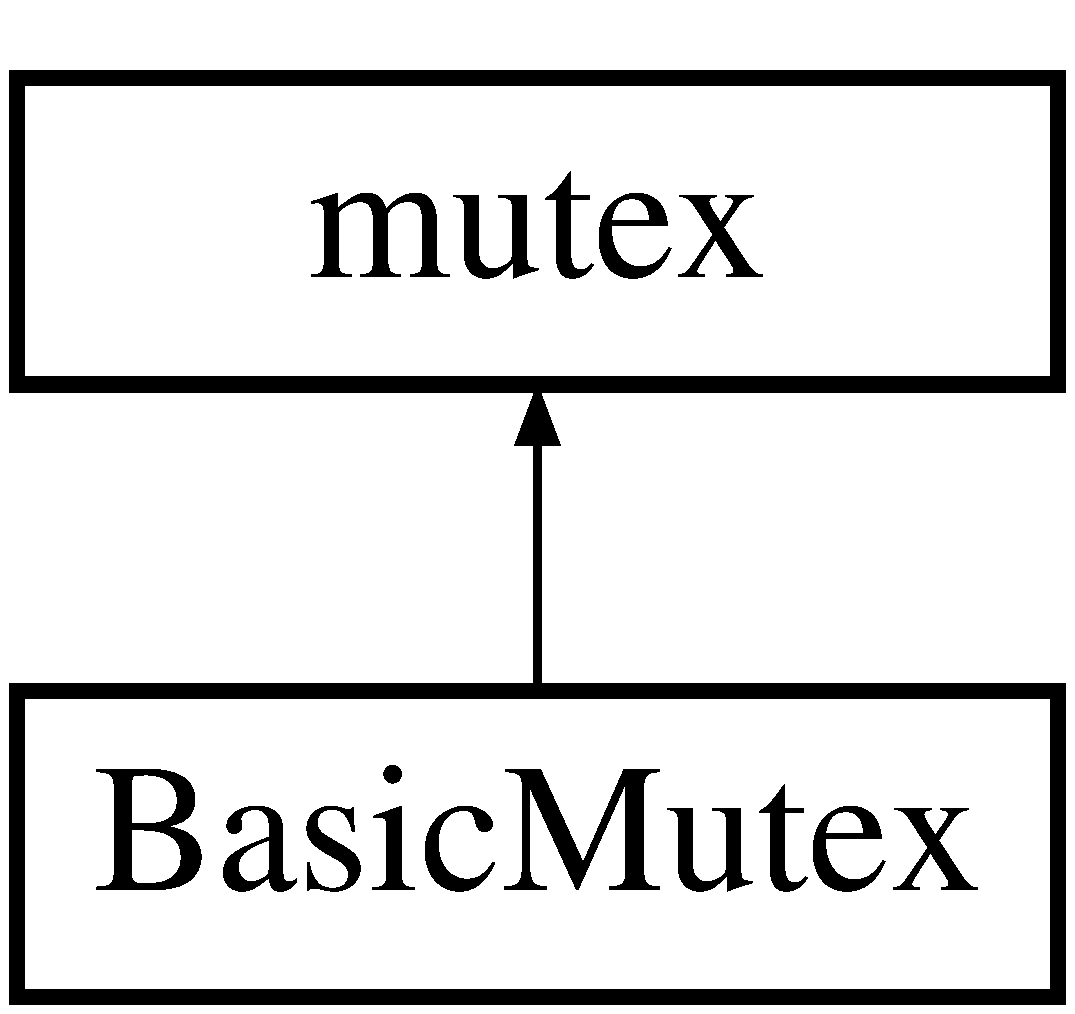
\includegraphics[height=2.000000cm]{class_basic_mutex}
\end{center}
\end{figure}
\subsection*{Public Member Functions}
\begin{DoxyCompactItemize}
\item 
\hyperlink{class_basic_mutex_aa578b7d25350cfdacf2245ac48f6c9a9}{Basic\-Mutex} ()
\item 
bool \hyperlink{class_basic_mutex_ad092a0e0ec88f115f29a6094b5e6c446}{is\-Locked} ()
\item 
void \hyperlink{class_basic_mutex_aa7a702cf99a4de227661cfb8604f2996}{lock} ()
\item 
bool \hyperlink{class_basic_mutex_a10ea86bf3ed7dc5b5e7fd98b456186ca}{try\-\_\-lock} () \-\_\-\-N\-O\-E\-X\-C\-E\-P\-T
\item 
void \hyperlink{class_basic_mutex_a2f14a0ea0347d8e1dd450301db0d4c34}{unlock} ()
\end{DoxyCompactItemize}
\subsection*{Protected Attributes}
\begin{DoxyCompactItemize}
\item 
bool \hyperlink{class_basic_mutex_a311753410a2191a3c6d5383698242ae9}{locked}
\end{DoxyCompactItemize}


\subsection{Detailed Description}


Definition at line 19 of file Basic\-Concurrency.\-h.



\subsection{Constructor \& Destructor Documentation}
\hypertarget{class_basic_mutex_aa578b7d25350cfdacf2245ac48f6c9a9}{\index{Basic\-Mutex@{Basic\-Mutex}!Basic\-Mutex@{Basic\-Mutex}}
\index{Basic\-Mutex@{Basic\-Mutex}!BasicMutex@{Basic\-Mutex}}
\subsubsection[{Basic\-Mutex}]{\setlength{\rightskip}{0pt plus 5cm}Basic\-Mutex\-::\-Basic\-Mutex (
\begin{DoxyParamCaption}
{}
\end{DoxyParamCaption}
)\hspace{0.3cm}{\ttfamily [inline]}}}\label{class_basic_mutex_aa578b7d25350cfdacf2245ac48f6c9a9}


Definition at line 27 of file Basic\-Concurrency.\-h.



\subsection{Member Function Documentation}
\hypertarget{class_basic_mutex_ad092a0e0ec88f115f29a6094b5e6c446}{\index{Basic\-Mutex@{Basic\-Mutex}!is\-Locked@{is\-Locked}}
\index{is\-Locked@{is\-Locked}!BasicMutex@{Basic\-Mutex}}
\subsubsection[{is\-Locked}]{\setlength{\rightskip}{0pt plus 5cm}bool Basic\-Mutex\-::is\-Locked (
\begin{DoxyParamCaption}
{}
\end{DoxyParamCaption}
)\hspace{0.3cm}{\ttfamily [inline]}}}\label{class_basic_mutex_ad092a0e0ec88f115f29a6094b5e6c446}


Definition at line 29 of file Basic\-Concurrency.\-h.

\hypertarget{class_basic_mutex_aa7a702cf99a4de227661cfb8604f2996}{\index{Basic\-Mutex@{Basic\-Mutex}!lock@{lock}}
\index{lock@{lock}!BasicMutex@{Basic\-Mutex}}
\subsubsection[{lock}]{\setlength{\rightskip}{0pt plus 5cm}void Basic\-Mutex\-::lock (
\begin{DoxyParamCaption}
{}
\end{DoxyParamCaption}
)}}\label{class_basic_mutex_aa7a702cf99a4de227661cfb8604f2996}


Definition at line 11 of file Basic\-Concurrency.\-cpp.

\hypertarget{class_basic_mutex_a10ea86bf3ed7dc5b5e7fd98b456186ca}{\index{Basic\-Mutex@{Basic\-Mutex}!try\-\_\-lock@{try\-\_\-lock}}
\index{try\-\_\-lock@{try\-\_\-lock}!BasicMutex@{Basic\-Mutex}}
\subsubsection[{try\-\_\-lock}]{\setlength{\rightskip}{0pt plus 5cm}bool Basic\-Mutex\-::try\-\_\-lock (
\begin{DoxyParamCaption}
{}
\end{DoxyParamCaption}
)}}\label{class_basic_mutex_a10ea86bf3ed7dc5b5e7fd98b456186ca}


Definition at line 16 of file Basic\-Concurrency.\-cpp.

\hypertarget{class_basic_mutex_a2f14a0ea0347d8e1dd450301db0d4c34}{\index{Basic\-Mutex@{Basic\-Mutex}!unlock@{unlock}}
\index{unlock@{unlock}!BasicMutex@{Basic\-Mutex}}
\subsubsection[{unlock}]{\setlength{\rightskip}{0pt plus 5cm}void Basic\-Mutex\-::unlock (
\begin{DoxyParamCaption}
{}
\end{DoxyParamCaption}
)}}\label{class_basic_mutex_a2f14a0ea0347d8e1dd450301db0d4c34}


Definition at line 21 of file Basic\-Concurrency.\-cpp.



\subsection{Member Data Documentation}
\hypertarget{class_basic_mutex_a311753410a2191a3c6d5383698242ae9}{\index{Basic\-Mutex@{Basic\-Mutex}!locked@{locked}}
\index{locked@{locked}!BasicMutex@{Basic\-Mutex}}
\subsubsection[{locked}]{\setlength{\rightskip}{0pt plus 5cm}bool Basic\-Mutex\-::locked\hspace{0.3cm}{\ttfamily [protected]}}}\label{class_basic_mutex_a311753410a2191a3c6d5383698242ae9}


Definition at line 23 of file Basic\-Concurrency.\-h.



The documentation for this class was generated from the following files\-:\begin{DoxyCompactItemize}
\item 
/\-Volumes/\-O\-S X H\-D\-D/\-Users/\-Adam/\-Developer/\-Sprite\-Fight/\-Util/\hyperlink{_basic_concurrency_8h}{Basic\-Concurrency.\-h}\item 
/\-Volumes/\-O\-S X H\-D\-D/\-Users/\-Adam/\-Developer/\-Sprite\-Fight/\-Util/\hyperlink{_basic_concurrency_8cpp}{Basic\-Concurrency.\-cpp}\end{DoxyCompactItemize}

\hypertarget{struct_bounds_check}{\section{Bounds\-Check$<$ N $>$ Struct Template Reference}
\label{struct_bounds_check}\index{Bounds\-Check$<$ N $>$@{Bounds\-Check$<$ N $>$}}
}


{\ttfamily \#include $<$Bounds\-Check.\-hpp$>$}

\subsection*{Public Member Functions}
\begin{DoxyCompactItemize}
\item 
\hyperlink{struct_bounds_check_a96b37a668190f8a77a839bf2db8d2018}{Bounds\-Check} (N min\-\_\-\-X\-\_\-, N max\-\_\-\-X\-\_\-, N min\-\_\-\-Y\-\_\-, N max\-\_\-\-Y\-\_\-)
\item 
void \hyperlink{struct_bounds_check_a658e5f4df28ce555de929f2098728289}{check\-Against} (N $\ast$x)
\item 
void \hyperlink{struct_bounds_check_af1535e1d5737008bc2fcccf295da21c8}{check\-Against} (N $\ast$x, N $\ast$y)
\end{DoxyCompactItemize}
\subsection*{Public Attributes}
\begin{DoxyCompactItemize}
\item 
const N \hyperlink{struct_bounds_check_a7ddafd0ac07f6ddfbd357f8bd440e952}{min\-\_\-\-X}
\item 
const N \hyperlink{struct_bounds_check_a8ed31dd874e9ee585a08018225adae4a}{max\-\_\-\-X}
\item 
const N \hyperlink{struct_bounds_check_ab70f0f1fe16a50a94c7e937ce892ef38}{min\-\_\-\-Y}
\item 
const N \hyperlink{struct_bounds_check_a569066d0fc5179aefddf172605682e72}{max\-\_\-\-Y}
\end{DoxyCompactItemize}
\subsection*{Static Public Attributes}
\begin{DoxyCompactItemize}
\item 
static \hyperlink{struct_bounds_check}{Bounds\-Check} \hyperlink{struct_bounds_check_abab10f32ac9cf636626694c004a0dcc7}{default\-Check}
\end{DoxyCompactItemize}


\subsection{Detailed Description}
\subsubsection*{template$<$typename N$>$struct Bounds\-Check$<$ N $>$}

Helps with checking validity of \hyperlink{struct_position}{Position} objects Used in \hyperlink{struct_position}{Position}'s check\-Bounds() 

Definition at line 22 of file Bounds\-Check.\-hpp.



\subsection{Constructor \& Destructor Documentation}
\hypertarget{struct_bounds_check_a96b37a668190f8a77a839bf2db8d2018}{\index{Bounds\-Check@{Bounds\-Check}!Bounds\-Check@{Bounds\-Check}}
\index{Bounds\-Check@{Bounds\-Check}!BoundsCheck@{Bounds\-Check}}
\subsubsection[{Bounds\-Check}]{\setlength{\rightskip}{0pt plus 5cm}template$<$typename N $>$ {\bf Bounds\-Check}$<$ N $>$\-::{\bf Bounds\-Check} (
\begin{DoxyParamCaption}
\item[{N}]{min\-\_\-\-X\-\_\-, }
\item[{N}]{max\-\_\-\-X\-\_\-, }
\item[{N}]{min\-\_\-\-Y\-\_\-, }
\item[{N}]{max\-\_\-\-Y\-\_\-}
\end{DoxyParamCaption}
)\hspace{0.3cm}{\ttfamily [inline]}}}\label{struct_bounds_check_a96b37a668190f8a77a839bf2db8d2018}


Definition at line 37 of file Bounds\-Check.\-hpp.



\subsection{Member Function Documentation}
\hypertarget{struct_bounds_check_a658e5f4df28ce555de929f2098728289}{\index{Bounds\-Check@{Bounds\-Check}!check\-Against@{check\-Against}}
\index{check\-Against@{check\-Against}!BoundsCheck@{Bounds\-Check}}
\subsubsection[{check\-Against}]{\setlength{\rightskip}{0pt plus 5cm}template$<$typename N $>$ void {\bf Bounds\-Check}$<$ N $>$\-::check\-Against (
\begin{DoxyParamCaption}
\item[{N $\ast$}]{x}
\end{DoxyParamCaption}
)\hspace{0.3cm}{\ttfamily [inline]}}}\label{struct_bounds_check_a658e5f4df28ce555de929f2098728289}


Definition at line 40 of file Bounds\-Check.\-hpp.

\hypertarget{struct_bounds_check_af1535e1d5737008bc2fcccf295da21c8}{\index{Bounds\-Check@{Bounds\-Check}!check\-Against@{check\-Against}}
\index{check\-Against@{check\-Against}!BoundsCheck@{Bounds\-Check}}
\subsubsection[{check\-Against}]{\setlength{\rightskip}{0pt plus 5cm}template$<$typename N $>$ void {\bf Bounds\-Check}$<$ N $>$\-::check\-Against (
\begin{DoxyParamCaption}
\item[{N $\ast$}]{x, }
\item[{N $\ast$}]{y}
\end{DoxyParamCaption}
)\hspace{0.3cm}{\ttfamily [inline]}}}\label{struct_bounds_check_af1535e1d5737008bc2fcccf295da21c8}


Definition at line 49 of file Bounds\-Check.\-hpp.



\subsection{Member Data Documentation}
\hypertarget{struct_bounds_check_abab10f32ac9cf636626694c004a0dcc7}{\index{Bounds\-Check@{Bounds\-Check}!default\-Check@{default\-Check}}
\index{default\-Check@{default\-Check}!BoundsCheck@{Bounds\-Check}}
\subsubsection[{default\-Check}]{\setlength{\rightskip}{0pt plus 5cm}template$<$typename N $>$ {\bf Bounds\-Check}$<$ N $>$ {\bf Bounds\-Check}$<$ N $>$\-::default\-Check\hspace{0.3cm}{\ttfamily [static]}}}\label{struct_bounds_check_abab10f32ac9cf636626694c004a0dcc7}


Definition at line 35 of file Bounds\-Check.\-hpp.

\hypertarget{struct_bounds_check_a8ed31dd874e9ee585a08018225adae4a}{\index{Bounds\-Check@{Bounds\-Check}!max\-\_\-\-X@{max\-\_\-\-X}}
\index{max\-\_\-\-X@{max\-\_\-\-X}!BoundsCheck@{Bounds\-Check}}
\subsubsection[{max\-\_\-\-X}]{\setlength{\rightskip}{0pt plus 5cm}template$<$typename N $>$ const N {\bf Bounds\-Check}$<$ N $>$\-::max\-\_\-\-X}}\label{struct_bounds_check_a8ed31dd874e9ee585a08018225adae4a}


Definition at line 31 of file Bounds\-Check.\-hpp.

\hypertarget{struct_bounds_check_a569066d0fc5179aefddf172605682e72}{\index{Bounds\-Check@{Bounds\-Check}!max\-\_\-\-Y@{max\-\_\-\-Y}}
\index{max\-\_\-\-Y@{max\-\_\-\-Y}!BoundsCheck@{Bounds\-Check}}
\subsubsection[{max\-\_\-\-Y}]{\setlength{\rightskip}{0pt plus 5cm}template$<$typename N $>$ const N {\bf Bounds\-Check}$<$ N $>$\-::max\-\_\-\-Y}}\label{struct_bounds_check_a569066d0fc5179aefddf172605682e72}


Definition at line 33 of file Bounds\-Check.\-hpp.

\hypertarget{struct_bounds_check_a7ddafd0ac07f6ddfbd357f8bd440e952}{\index{Bounds\-Check@{Bounds\-Check}!min\-\_\-\-X@{min\-\_\-\-X}}
\index{min\-\_\-\-X@{min\-\_\-\-X}!BoundsCheck@{Bounds\-Check}}
\subsubsection[{min\-\_\-\-X}]{\setlength{\rightskip}{0pt plus 5cm}template$<$typename N $>$ const N {\bf Bounds\-Check}$<$ N $>$\-::min\-\_\-\-X}}\label{struct_bounds_check_a7ddafd0ac07f6ddfbd357f8bd440e952}


Definition at line 30 of file Bounds\-Check.\-hpp.

\hypertarget{struct_bounds_check_ab70f0f1fe16a50a94c7e937ce892ef38}{\index{Bounds\-Check@{Bounds\-Check}!min\-\_\-\-Y@{min\-\_\-\-Y}}
\index{min\-\_\-\-Y@{min\-\_\-\-Y}!BoundsCheck@{Bounds\-Check}}
\subsubsection[{min\-\_\-\-Y}]{\setlength{\rightskip}{0pt plus 5cm}template$<$typename N $>$ const N {\bf Bounds\-Check}$<$ N $>$\-::min\-\_\-\-Y}}\label{struct_bounds_check_ab70f0f1fe16a50a94c7e937ce892ef38}


Definition at line 32 of file Bounds\-Check.\-hpp.



The documentation for this struct was generated from the following file\-:\begin{DoxyCompactItemize}
\item 
/\-Volumes/\-O\-S X H\-D\-D/\-Users/\-Adam/\-Developer/\-Sprite\-Fight/\-Util/\hyperlink{_bounds_check_8hpp}{Bounds\-Check.\-hpp}\end{DoxyCompactItemize}

\hypertarget{class_character}{\section{Character Class Reference}
\label{class_character}\index{Character@{Character}}
}


A class which serves as the basic template for just about any person in the game world, whether player or npc.  




{\ttfamily \#include $<$Character.\-h$>$}

Inheritance diagram for Character\-:\begin{figure}[H]
\begin{center}
\leavevmode
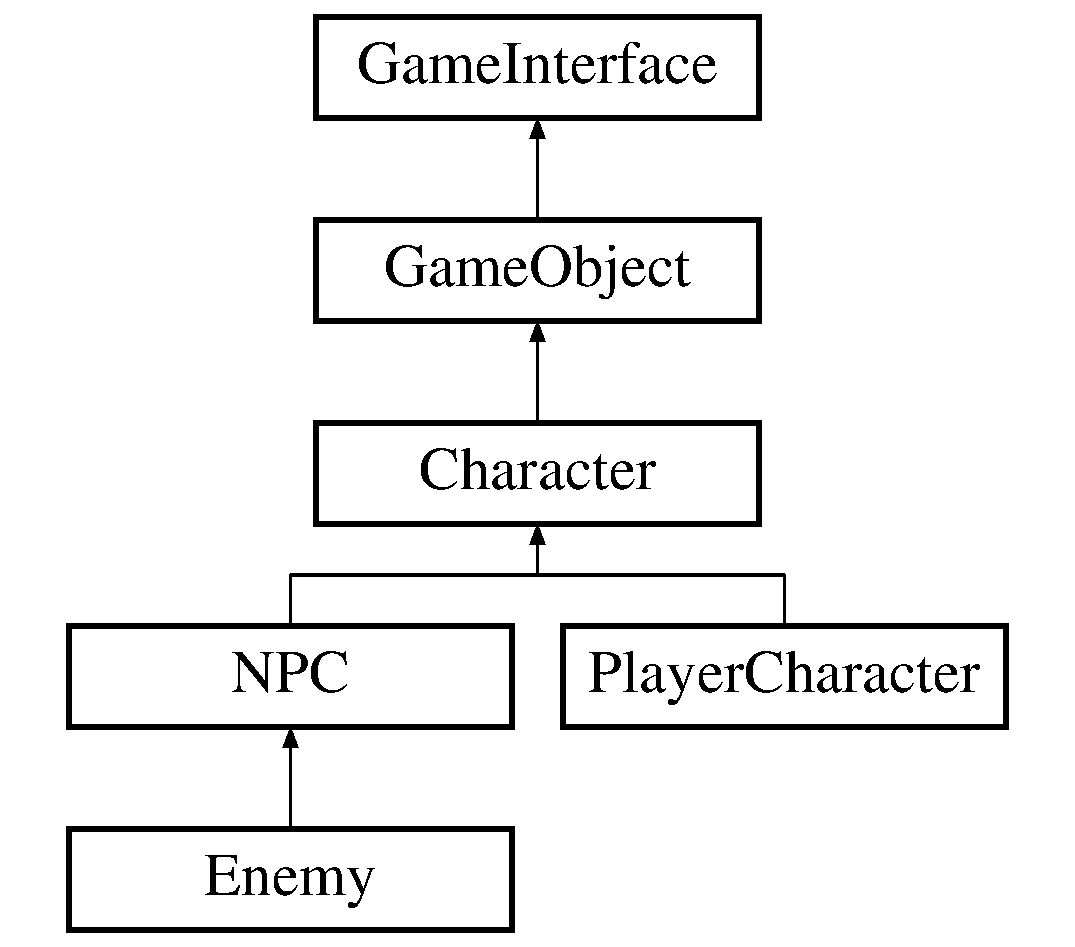
\includegraphics[height=5.000000cm]{class_character}
\end{center}
\end{figure}
\subsection*{Public Member Functions}
\begin{DoxyCompactItemize}
\item 
\hyperlink{class_character_adc27bdd255876169bad2ed0bae0cffb5}{Character} ()
\begin{DoxyCompactList}\small\item\em Constructs a default \hyperlink{class_character}{Character}. \end{DoxyCompactList}\item 
\hyperlink{class_character_a0eac14bff9a793857bb2a86a2c0fcf9c}{Character} (const \hyperlink{class_character}{Character} \&other)
\item 
\hyperlink{class_character_a90171e1a0ff378b3bbe125f85b4ecfdb}{Character} (\hyperlink{class_character}{Character} \&\&other)
\item 
\hyperlink{class_character_a71ddaf9372427d6bacf3b6aa0116cecf}{Character} (const \hyperlink{struct_asset_file}{Asset\-File} \&image\-File, float size\-Modifier, const \hyperlink{struct_position}{Position}$<$ float $>$ \&\hyperlink{class_game_object_a6858e668e7d2c5ded850b952aaacd905}{loc}, string \hyperlink{class_character_a2d423654566d1bf2160fef74bf04cc84}{name}, \hyperlink{_character_data_8h_a0e5ce1612c1e71823c97a9cd734de339}{Reaction} \hyperlink{class_character_a579933775b2e4e97465bacb09c4e87f5}{reaction}, \hyperlink{_character_data_8h_acbff4d7298e294294555d39178aad448}{Do\-A} \hyperlink{class_character_ac83b99be690bb41b7fae53e9457838c6}{alive}, \hyperlink{_character_data_8h_aacbb008a93d24b04a8779bbdbd8880b5}{Character\-State} \hyperlink{class_character_ac20f1ebda238017ddc245ecdce827037}{state}, unsigned \hyperlink{class_character_ae8c0d82624dc3a171e2c3b42c699151e}{health}, unsigned \hyperlink{class_character_ae6a140637ffe5004179d90a0e04a411b}{damage}, bool monitor\-Velocity)
\item 
\hyperlink{class_character_aa9363d80872be14d29b006745ff0b58a}{Character} (\hyperlink{class_fast_rand}{Fast\-Rand}$<$ int $>$ rand)
\item 
\hyperlink{class_character_a9e9be564d05ded80962b2045aa70b3fc}{$\sim$\-Character} ()
\item 
virtual \hyperlink{class_character}{Character} \& \hyperlink{class_character_acdb4f61692995622e350cbfbb0c4d8c6}{operator=} (const \hyperlink{class_character}{Character} \&rhs)
\item 
virtual \hyperlink{class_character}{Character} \& \hyperlink{class_character_a0c0f1e362dabc8877889e49185afd43e}{operator=} (\hyperlink{class_character}{Character} \&\&rhs)
\item 
virtual void \hyperlink{class_character_a3c4dfc59865fe39251070cd0b92d34ac}{operator()} ()
\item 
virtual void \hyperlink{class_character_a6dde2dd17bfd31ea6e008d83bdcd3188}{operator()} (\hyperlink{class_game_object}{Game\-Object} $\ast$other)
\item 
virtual void \hyperlink{class_character_a457dab4f04550716888425da681b9f1f}{notify} ()
\item 
virtual void \hyperlink{class_character_ad0574321c7429301d4d9dd1dd33301c4}{pass\-Message} (\hyperlink{struct_message}{Message} $\ast$message, \hyperlink{class_game_object}{Game\-Object} \&recipient)
\item 
virtual void \hyperlink{class_character_a2ab1090f959f0c66b098e0463d4c1bdd}{text\-Description} (ostream $\ast$write\-To) const 
\item 
virtual void \hyperlink{class_character_ac96260f4fd9b68a33919a65bc9da9bca}{default\-Behaviors} () override
\item 
virtual void \hyperlink{class_character_a7bd55d3615c1eb092f800d8634fa9695}{ai\-Behaviors} () override
\item 
virtual void \hyperlink{class_character_a7be3b65a2bc5facbb39ee208f5898560}{attack} (\hyperlink{class_character}{Character} $\ast$enemy)
\item 
const string \& \hyperlink{class_character_afb6ef570e4bfc7f1d81ead9ed7e4c744}{get\-Name} () const 
\item 
void \hyperlink{class_character_a9bf101bdd0a5cf667f058da2c66f989b}{set\-Name} (string s)
\begin{DoxyCompactList}\small\item\em Setter for name. \end{DoxyCompactList}\item 
\hyperlink{_character_data_8h_aacbb008a93d24b04a8779bbdbd8880b5}{Character\-State} $\ast$ \hyperlink{class_character_a1887dada668e71e5b072e71178df87b0}{get\-State} ()
\item 
void \hyperlink{class_character_ae3a8fe67a8b3761322a448468c6a0b09}{set\-State} (\hyperlink{_character_data_8h_aacbb008a93d24b04a8779bbdbd8880b5}{Character\-State} \&\hyperlink{class_character_ac20f1ebda238017ddc245ecdce827037}{state})
\item 
\hyperlink{struct_health}{Health} $\ast$ \hyperlink{class_character_a225fa5b49f3330f70936ece3f6993448}{check\-Health} ()
\item 
void \hyperlink{class_character_a22d3d47dcf5775dac41539ecc3dee072}{mod\-Health} (\hyperlink{struct_health}{Health} $\ast$)
\item 
\hyperlink{struct_damage}{Damage} $\ast$ \hyperlink{class_character_a180960a01e928627bfd672dbb19b2f56}{get\-Damage} ()
\item 
void \hyperlink{class_character_a80e7bdfad72a223ff4a98e45089ea896}{mod\-Damage} (\hyperlink{struct_damage}{Damage} $\ast$)
\end{DoxyCompactItemize}
\subsection*{Protected Member Functions}
\begin{DoxyCompactItemize}
\item 
void \hyperlink{class_character_aa3a40043d1f3c27edd921aa0e0ef7616}{attack\-\_\-helper} (\hyperlink{class_character}{Character} $\ast$enemy)
\end{DoxyCompactItemize}
\subsection*{Protected Attributes}
\begin{DoxyCompactItemize}
\item 
string \hyperlink{class_character_a2d423654566d1bf2160fef74bf04cc84}{name}
\item 
\hyperlink{_character_data_8h_a0e5ce1612c1e71823c97a9cd734de339}{Reaction} \hyperlink{class_character_a579933775b2e4e97465bacb09c4e87f5}{reaction}
\item 
\hyperlink{_character_data_8h_acbff4d7298e294294555d39178aad448}{Do\-A} \hyperlink{class_character_ac83b99be690bb41b7fae53e9457838c6}{alive}
\item 
\hyperlink{_character_data_8h_aacbb008a93d24b04a8779bbdbd8880b5}{Character\-State} \hyperlink{class_character_ac20f1ebda238017ddc245ecdce827037}{state}
\item 
\hyperlink{struct_health}{Health} $\ast$ \hyperlink{class_character_ae8c0d82624dc3a171e2c3b42c699151e}{health}
\item 
\hyperlink{struct_damage}{Damage} $\ast$ \hyperlink{class_character_ae6a140637ffe5004179d90a0e04a411b}{damage}
\item 
bool \hyperlink{class_character_a5195d893143824d0ba34180a94229543}{turn} = false
\item 
float \hyperlink{class_character_a6328c239882a3c7794332d24d100e02d}{hit\-Percentage}
\end{DoxyCompactItemize}
\subsection*{Additional Inherited Members}


\subsection{Detailed Description}
A class which serves as the basic template for just about any person in the game world, whether player or npc. 

Definition at line 23 of file Character.\-h.



\subsection{Constructor \& Destructor Documentation}
\hypertarget{class_character_adc27bdd255876169bad2ed0bae0cffb5}{\index{Character@{Character}!Character@{Character}}
\index{Character@{Character}!Character@{Character}}
\subsubsection[{Character}]{\setlength{\rightskip}{0pt plus 5cm}Character\-::\-Character (
\begin{DoxyParamCaption}
{}
\end{DoxyParamCaption}
)}}\label{class_character_adc27bdd255876169bad2ed0bae0cffb5}


Constructs a default \hyperlink{class_character}{Character}. 



Definition at line 12 of file Character.\-cpp.

\hypertarget{class_character_a0eac14bff9a793857bb2a86a2c0fcf9c}{\index{Character@{Character}!Character@{Character}}
\index{Character@{Character}!Character@{Character}}
\subsubsection[{Character}]{\setlength{\rightskip}{0pt plus 5cm}Character\-::\-Character (
\begin{DoxyParamCaption}
\item[{const {\bf Character} \&}]{other}
\end{DoxyParamCaption}
)}}\label{class_character_a0eac14bff9a793857bb2a86a2c0fcf9c}
Copy constructor for \hyperlink{class_character}{Character}


\begin{DoxyParams}{Parameters}
{\em other} & \hyperlink{class_character}{Character} to be copied \\
\hline
\end{DoxyParams}


Definition at line 20 of file Character.\-cpp.

\hypertarget{class_character_a90171e1a0ff378b3bbe125f85b4ecfdb}{\index{Character@{Character}!Character@{Character}}
\index{Character@{Character}!Character@{Character}}
\subsubsection[{Character}]{\setlength{\rightskip}{0pt plus 5cm}Character\-::\-Character (
\begin{DoxyParamCaption}
\item[{{\bf Character} \&\&}]{other}
\end{DoxyParamCaption}
)}}\label{class_character_a90171e1a0ff378b3bbe125f85b4ecfdb}
Move constructor for \hyperlink{class_character}{Character}


\begin{DoxyParams}{Parameters}
{\em other} & \hyperlink{class_character}{Character} to be moved \\
\hline
\end{DoxyParams}


Definition at line 28 of file Character.\-cpp.

\hypertarget{class_character_a71ddaf9372427d6bacf3b6aa0116cecf}{\index{Character@{Character}!Character@{Character}}
\index{Character@{Character}!Character@{Character}}
\subsubsection[{Character}]{\setlength{\rightskip}{0pt plus 5cm}Character\-::\-Character (
\begin{DoxyParamCaption}
\item[{const {\bf Asset\-File} \&}]{image\-File, }
\item[{float}]{size\-Modifier, }
\item[{const {\bf Position}$<$ float $>$ \&}]{loc, }
\item[{string}]{name, }
\item[{{\bf Reaction}}]{reaction, }
\item[{{\bf Do\-A}}]{alive, }
\item[{{\bf Character\-State}}]{state, }
\item[{unsigned}]{health, }
\item[{unsigned}]{damage, }
\item[{bool}]{monitor\-Velocity}
\end{DoxyParamCaption}
)}}\label{class_character_a71ddaf9372427d6bacf3b6aa0116cecf}
Constructs a \hyperlink{class_character}{Character} based on the arguments given


\begin{DoxyParams}{Parameters}
{\em name} & The name of this \hyperlink{class_character}{Character} \\
\hline
{\em alive} & Whether this \hyperlink{class_character}{Character} is dead or alive \\
\hline
{\em state} & The Character\-State of this \hyperlink{class_character}{Character} \\
\hline
{\em health} & The \hyperlink{struct_health}{Health} of this \hyperlink{class_character}{Character} \\
\hline
{\em damage} & The \hyperlink{struct_damage}{Damage} capability of this \hyperlink{class_character}{Character} \\
\hline
\end{DoxyParams}


Definition at line 40 of file Character.\-cpp.

\hypertarget{class_character_aa9363d80872be14d29b006745ff0b58a}{\index{Character@{Character}!Character@{Character}}
\index{Character@{Character}!Character@{Character}}
\subsubsection[{Character}]{\setlength{\rightskip}{0pt plus 5cm}Character\-::\-Character (
\begin{DoxyParamCaption}
\item[{{\bf Fast\-Rand}$<$ int $>$}]{rand}
\end{DoxyParamCaption}
)}}\label{class_character_aa9363d80872be14d29b006745ff0b58a}
Constructs a randomized \hyperlink{class_character}{Character}. The client has to option to simply leave the argument rand\-Seed as 0, in which case the constructor will generate its own random number.


\begin{DoxyParams}{Parameters}
{\em rand} & A seed to initialize the random number generator \\
\hline
\end{DoxyParams}


Definition at line 47 of file Character.\-cpp.

\hypertarget{class_character_a9e9be564d05ded80962b2045aa70b3fc}{\index{Character@{Character}!$\sim$\-Character@{$\sim$\-Character}}
\index{$\sim$\-Character@{$\sim$\-Character}!Character@{Character}}
\subsubsection[{$\sim$\-Character}]{\setlength{\rightskip}{0pt plus 5cm}Character\-::$\sim$\-Character (
\begin{DoxyParamCaption}
{}
\end{DoxyParamCaption}
)}}\label{class_character_a9e9be564d05ded80962b2045aa70b3fc}
Destructor for \hyperlink{class_character}{Character} 

Definition at line 58 of file Character.\-cpp.



\subsection{Member Function Documentation}
\hypertarget{class_character_a7bd55d3615c1eb092f800d8634fa9695}{\index{Character@{Character}!ai\-Behaviors@{ai\-Behaviors}}
\index{ai\-Behaviors@{ai\-Behaviors}!Character@{Character}}
\subsubsection[{ai\-Behaviors}]{\setlength{\rightskip}{0pt plus 5cm}void Character\-::ai\-Behaviors (
\begin{DoxyParamCaption}
{}
\end{DoxyParamCaption}
)\hspace{0.3cm}{\ttfamily [override]}, {\ttfamily [virtual]}}}\label{class_character_a7bd55d3615c1eb092f800d8634fa9695}


Reimplemented from \hyperlink{class_game_object_a43862b5d602a0fec32b686ab8586e886}{Game\-Object}.



Reimplemented in \hyperlink{class_player_character_af7a8c30b3f40a698c28b095a299657ab}{Player\-Character}.



Definition at line 127 of file Character.\-cpp.

\hypertarget{class_character_a7be3b65a2bc5facbb39ee208f5898560}{\index{Character@{Character}!attack@{attack}}
\index{attack@{attack}!Character@{Character}}
\subsubsection[{attack}]{\setlength{\rightskip}{0pt plus 5cm}void Character\-::attack (
\begin{DoxyParamCaption}
\item[{{\bf Character} $\ast$}]{enemy}
\end{DoxyParamCaption}
)\hspace{0.3cm}{\ttfamily [virtual]}}}\label{class_character_a7be3b65a2bc5facbb39ee208f5898560}
Attacks a hostile \hyperlink{class_character}{Character}


\begin{DoxyParams}{Parameters}
{\em enemy} & The enemy to attack \\
\hline
\end{DoxyParams}


Reimplemented in \hyperlink{class_n_p_c_a35234d189d4b9dee193b49f3d9272a0e}{N\-P\-C}.



Definition at line 132 of file Character.\-cpp.

\hypertarget{class_character_aa3a40043d1f3c27edd921aa0e0ef7616}{\index{Character@{Character}!attack\-\_\-helper@{attack\-\_\-helper}}
\index{attack\-\_\-helper@{attack\-\_\-helper}!Character@{Character}}
\subsubsection[{attack\-\_\-helper}]{\setlength{\rightskip}{0pt plus 5cm}void Character\-::attack\-\_\-helper (
\begin{DoxyParamCaption}
\item[{{\bf Character} $\ast$}]{enemy}
\end{DoxyParamCaption}
)\hspace{0.3cm}{\ttfamily [protected]}}}\label{class_character_aa3a40043d1f3c27edd921aa0e0ef7616}


Definition at line 157 of file Character.\-cpp.

\hypertarget{class_character_a225fa5b49f3330f70936ece3f6993448}{\index{Character@{Character}!check\-Health@{check\-Health}}
\index{check\-Health@{check\-Health}!Character@{Character}}
\subsubsection[{check\-Health}]{\setlength{\rightskip}{0pt plus 5cm}{\bf Health} $\ast$ Character\-::check\-Health (
\begin{DoxyParamCaption}
{}
\end{DoxyParamCaption}
)}}\label{class_character_a225fa5b49f3330f70936ece3f6993448}
\begin{DoxyReturn}{Returns}
a value representing \hyperlink{class_character}{Character}'s health 
\end{DoxyReturn}


Definition at line 177 of file Character.\-cpp.

\hypertarget{class_character_ac96260f4fd9b68a33919a65bc9da9bca}{\index{Character@{Character}!default\-Behaviors@{default\-Behaviors}}
\index{default\-Behaviors@{default\-Behaviors}!Character@{Character}}
\subsubsection[{default\-Behaviors}]{\setlength{\rightskip}{0pt plus 5cm}void Character\-::default\-Behaviors (
\begin{DoxyParamCaption}
{}
\end{DoxyParamCaption}
)\hspace{0.3cm}{\ttfamily [override]}, {\ttfamily [virtual]}}}\label{class_character_ac96260f4fd9b68a33919a65bc9da9bca}
Each \hyperlink{class_game_object}{Game\-Object} can implement this to enable its default behaviors to run on a loop on a separate thread 

Reimplemented from \hyperlink{class_game_object_a565a3950ea0af84bf7515bdb77abf51a}{Game\-Object}.



Reimplemented in \hyperlink{class_player_character_ac96dd84cef7668557321edc5b251c97c}{Player\-Character}, and \hyperlink{class_enemy_acec008d64103ef820006bcbcf9345a2a}{Enemy}.



Definition at line 123 of file Character.\-cpp.

\hypertarget{class_character_a180960a01e928627bfd672dbb19b2f56}{\index{Character@{Character}!get\-Damage@{get\-Damage}}
\index{get\-Damage@{get\-Damage}!Character@{Character}}
\subsubsection[{get\-Damage}]{\setlength{\rightskip}{0pt plus 5cm}{\bf Damage} $\ast$ Character\-::get\-Damage (
\begin{DoxyParamCaption}
{}
\end{DoxyParamCaption}
)}}\label{class_character_a180960a01e928627bfd672dbb19b2f56}
\begin{DoxyReturn}{Returns}
a read-\/only value representing \hyperlink{class_character}{Character}'s damage 
\end{DoxyReturn}


Definition at line 189 of file Character.\-cpp.

\hypertarget{class_character_afb6ef570e4bfc7f1d81ead9ed7e4c744}{\index{Character@{Character}!get\-Name@{get\-Name}}
\index{get\-Name@{get\-Name}!Character@{Character}}
\subsubsection[{get\-Name}]{\setlength{\rightskip}{0pt plus 5cm}const string\& Character\-::get\-Name (
\begin{DoxyParamCaption}
{}
\end{DoxyParamCaption}
) const\hspace{0.3cm}{\ttfamily [inline]}}}\label{class_character_afb6ef570e4bfc7f1d81ead9ed7e4c744}
Getter for name 

Definition at line 174 of file Character.\-h.

\hypertarget{class_character_a1887dada668e71e5b072e71178df87b0}{\index{Character@{Character}!get\-State@{get\-State}}
\index{get\-State@{get\-State}!Character@{Character}}
\subsubsection[{get\-State}]{\setlength{\rightskip}{0pt plus 5cm}{\bf Character\-State} $\ast$ Character\-::get\-State (
\begin{DoxyParamCaption}
{}
\end{DoxyParamCaption}
)}}\label{class_character_a1887dada668e71e5b072e71178df87b0}
\begin{DoxyReturn}{Returns}
This character's current state 
\end{DoxyReturn}


Definition at line 172 of file Character.\-cpp.

\hypertarget{class_character_a80e7bdfad72a223ff4a98e45089ea896}{\index{Character@{Character}!mod\-Damage@{mod\-Damage}}
\index{mod\-Damage@{mod\-Damage}!Character@{Character}}
\subsubsection[{mod\-Damage}]{\setlength{\rightskip}{0pt plus 5cm}void Character\-::mod\-Damage (
\begin{DoxyParamCaption}
\item[{{\bf Damage} $\ast$}]{other}
\end{DoxyParamCaption}
)}}\label{class_character_a80e7bdfad72a223ff4a98e45089ea896}
Sets this \hyperlink{class_character}{Character}'s damage 

Definition at line 194 of file Character.\-cpp.

\hypertarget{class_character_a22d3d47dcf5775dac41539ecc3dee072}{\index{Character@{Character}!mod\-Health@{mod\-Health}}
\index{mod\-Health@{mod\-Health}!Character@{Character}}
\subsubsection[{mod\-Health}]{\setlength{\rightskip}{0pt plus 5cm}void Character\-::mod\-Health (
\begin{DoxyParamCaption}
\item[{{\bf Health} $\ast$}]{other}
\end{DoxyParamCaption}
)}}\label{class_character_a22d3d47dcf5775dac41539ecc3dee072}
Sets this \hyperlink{class_character}{Character}'s health 

Definition at line 183 of file Character.\-cpp.

\hypertarget{class_character_a457dab4f04550716888425da681b9f1f}{\index{Character@{Character}!notify@{notify}}
\index{notify@{notify}!Character@{Character}}
\subsubsection[{notify}]{\setlength{\rightskip}{0pt plus 5cm}void Character\-::notify (
\begin{DoxyParamCaption}
{}
\end{DoxyParamCaption}
)\hspace{0.3cm}{\ttfamily [virtual]}}}\label{class_character_a457dab4f04550716888425da681b9f1f}
Another class with a reference to this \hyperlink{class_character}{Character} can call this to have the \hyperlink{class_character}{Character} perform some function, as yet undecided. T\-B\-I. 

Reimplemented from \hyperlink{class_game_object_a9867e75f8cfc4df52d03467aca07a4ac}{Game\-Object}.



Reimplemented in \hyperlink{class_n_p_c_ab590b71db4dd9dc21f6e2c183e9bd45c}{N\-P\-C}.



Definition at line 104 of file Character.\-cpp.

\hypertarget{class_character_a3c4dfc59865fe39251070cd0b92d34ac}{\index{Character@{Character}!operator()@{operator()}}
\index{operator()@{operator()}!Character@{Character}}
\subsubsection[{operator()}]{\setlength{\rightskip}{0pt plus 5cm}void Character\-::operator() (
\begin{DoxyParamCaption}
{}
\end{DoxyParamCaption}
)\hspace{0.3cm}{\ttfamily [virtual]}}}\label{class_character_a3c4dfc59865fe39251070cd0b92d34ac}
Overloads operator() for \hyperlink{class_character}{Character}. Possibly will be used to call \hyperlink{class_character_a457dab4f04550716888425da681b9f1f}{notify()}. T\-B\-D. 

Reimplemented from \hyperlink{class_game_object_ab8fccd5edcbebad0553aa4336a71452a}{Game\-Object}.



Reimplemented in \hyperlink{class_player_character_a067c5b11f7deafd448726ec4ac294b03}{Player\-Character}, and \hyperlink{class_n_p_c_a73befe685fef40ab7f1ac954d932697d}{N\-P\-C}.



Definition at line 96 of file Character.\-cpp.

\hypertarget{class_character_a6dde2dd17bfd31ea6e008d83bdcd3188}{\index{Character@{Character}!operator()@{operator()}}
\index{operator()@{operator()}!Character@{Character}}
\subsubsection[{operator()}]{\setlength{\rightskip}{0pt plus 5cm}void Character\-::operator() (
\begin{DoxyParamCaption}
\item[{{\bf Game\-Object} $\ast$}]{other}
\end{DoxyParamCaption}
)\hspace{0.3cm}{\ttfamily [virtual]}}}\label{class_character_a6dde2dd17bfd31ea6e008d83bdcd3188}
Overloads the overload of operator(). The actual implementation and uses for this are still undecided.


\begin{DoxyParams}{Parameters}
{\em other} & A reference to another \hyperlink{class_character}{Character} \\
\hline
\end{DoxyParams}


Reimplemented from \hyperlink{class_game_object_afe9e6ee87d3062c80a9c560a12bfc279}{Game\-Object}.



Reimplemented in \hyperlink{class_player_character_a1cf7079c60a26c188cf4ed7043a2c9b3}{Player\-Character}.



Definition at line 100 of file Character.\-cpp.

\hypertarget{class_character_acdb4f61692995622e350cbfbb0c4d8c6}{\index{Character@{Character}!operator=@{operator=}}
\index{operator=@{operator=}!Character@{Character}}
\subsubsection[{operator=}]{\setlength{\rightskip}{0pt plus 5cm}{\bf Character} \& Character\-::operator= (
\begin{DoxyParamCaption}
\item[{const {\bf Character} \&}]{rhs}
\end{DoxyParamCaption}
)\hspace{0.3cm}{\ttfamily [virtual]}}}\label{class_character_acdb4f61692995622e350cbfbb0c4d8c6}
Assignment operator overload (copy)


\begin{DoxyParams}{Parameters}
{\em rhs} & The right hand side argument (which will be copied) \\
\hline
\end{DoxyParams}


Definition at line 67 of file Character.\-cpp.

\hypertarget{class_character_a0c0f1e362dabc8877889e49185afd43e}{\index{Character@{Character}!operator=@{operator=}}
\index{operator=@{operator=}!Character@{Character}}
\subsubsection[{operator=}]{\setlength{\rightskip}{0pt plus 5cm}{\bf Character} \& Character\-::operator= (
\begin{DoxyParamCaption}
\item[{{\bf Character} \&\&}]{rhs}
\end{DoxyParamCaption}
)\hspace{0.3cm}{\ttfamily [virtual]}}}\label{class_character_a0c0f1e362dabc8877889e49185afd43e}
Assignment operator overload (move)


\begin{DoxyParams}{Parameters}
{\em rhs} & The right hand side argument (which will be moved) \\
\hline
\end{DoxyParams}


Definition at line 80 of file Character.\-cpp.

\hypertarget{class_character_ad0574321c7429301d4d9dd1dd33301c4}{\index{Character@{Character}!pass\-Message@{pass\-Message}}
\index{pass\-Message@{pass\-Message}!Character@{Character}}
\subsubsection[{pass\-Message}]{\setlength{\rightskip}{0pt plus 5cm}void Character\-::pass\-Message (
\begin{DoxyParamCaption}
\item[{{\bf Message} $\ast$}]{message, }
\item[{{\bf Game\-Object} \&}]{recipient}
\end{DoxyParamCaption}
)\hspace{0.3cm}{\ttfamily [virtual]}}}\label{class_character_ad0574321c7429301d4d9dd1dd33301c4}
A \hyperlink{class_character}{Character} can use this function to pass messages to another.


\begin{DoxyParams}{Parameters}
{\em message} & The \hyperlink{struct_message}{Message} sent by this \\
\hline
{\em recipient} & The object receiving the \hyperlink{struct_message}{Message} \\
\hline
\end{DoxyParams}


Reimplemented from \hyperlink{class_game_object_ad7f752f1e3c84bd74de6110c17df3938}{Game\-Object}.



Definition at line 108 of file Character.\-cpp.

\hypertarget{class_character_a9bf101bdd0a5cf667f058da2c66f989b}{\index{Character@{Character}!set\-Name@{set\-Name}}
\index{set\-Name@{set\-Name}!Character@{Character}}
\subsubsection[{set\-Name}]{\setlength{\rightskip}{0pt plus 5cm}void Character\-::set\-Name (
\begin{DoxyParamCaption}
\item[{string}]{s}
\end{DoxyParamCaption}
)\hspace{0.3cm}{\ttfamily [inline]}}}\label{class_character_a9bf101bdd0a5cf667f058da2c66f989b}


Setter for name. 


\begin{DoxyParams}{Parameters}
{\em s} & The \hyperlink{class_character}{Character}'s new name \\
\hline
\end{DoxyParams}


Definition at line 181 of file Character.\-h.

\hypertarget{class_character_ae3a8fe67a8b3761322a448468c6a0b09}{\index{Character@{Character}!set\-State@{set\-State}}
\index{set\-State@{set\-State}!Character@{Character}}
\subsubsection[{set\-State}]{\setlength{\rightskip}{0pt plus 5cm}void Character\-::set\-State (
\begin{DoxyParamCaption}
\item[{{\bf Character\-State} \&}]{state}
\end{DoxyParamCaption}
)\hspace{0.3cm}{\ttfamily [inline]}}}\label{class_character_ae3a8fe67a8b3761322a448468c6a0b09}
Set's this \hyperlink{class_character}{Character}'s state


\begin{DoxyParams}{Parameters}
{\em state} & The \hyperlink{class_character}{Character}'s new state \\
\hline
\end{DoxyParams}


Definition at line 193 of file Character.\-h.

\hypertarget{class_character_a2ab1090f959f0c66b098e0463d4c1bdd}{\index{Character@{Character}!text\-Description@{text\-Description}}
\index{text\-Description@{text\-Description}!Character@{Character}}
\subsubsection[{text\-Description}]{\setlength{\rightskip}{0pt plus 5cm}void Character\-::text\-Description (
\begin{DoxyParamCaption}
\item[{ostream $\ast$}]{write\-To}
\end{DoxyParamCaption}
) const\hspace{0.3cm}{\ttfamily [virtual]}}}\label{class_character_a2ab1090f959f0c66b098e0463d4c1bdd}
Writes a formatted text description of this \hyperlink{class_character}{Character} into the desired output stream 

Reimplemented from \hyperlink{class_game_object_adc249c683994a9c74b518a82fc22dbab}{Game\-Object}.



Reimplemented in \hyperlink{class_player_character_aac83579c2f552973e71008c1b1e01b1d}{Player\-Character}, and \hyperlink{class_n_p_c_ad85699c2a35f1f5f9d5a81a3d5df2153}{N\-P\-C}.



Definition at line 112 of file Character.\-cpp.



\subsection{Member Data Documentation}
\hypertarget{class_character_ac83b99be690bb41b7fae53e9457838c6}{\index{Character@{Character}!alive@{alive}}
\index{alive@{alive}!Character@{Character}}
\subsubsection[{alive}]{\setlength{\rightskip}{0pt plus 5cm}{\bf Do\-A} Character\-::alive\hspace{0.3cm}{\ttfamily [protected]}}}\label{class_character_ac83b99be690bb41b7fae53e9457838c6}


Definition at line 31 of file Character.\-h.

\hypertarget{class_character_ae6a140637ffe5004179d90a0e04a411b}{\index{Character@{Character}!damage@{damage}}
\index{damage@{damage}!Character@{Character}}
\subsubsection[{damage}]{\setlength{\rightskip}{0pt plus 5cm}{\bf Damage}$\ast$ Character\-::damage\hspace{0.3cm}{\ttfamily [protected]}}}\label{class_character_ae6a140637ffe5004179d90a0e04a411b}
The \hyperlink{class_character}{Character}'s current \hyperlink{struct_damage}{Damage} (a data structure inheriting from \hyperlink{struct_game_state}{Game\-State}) 

Definition at line 46 of file Character.\-h.

\hypertarget{class_character_ae8c0d82624dc3a171e2c3b42c699151e}{\index{Character@{Character}!health@{health}}
\index{health@{health}!Character@{Character}}
\subsubsection[{health}]{\setlength{\rightskip}{0pt plus 5cm}{\bf Health}$\ast$ Character\-::health\hspace{0.3cm}{\ttfamily [protected]}}}\label{class_character_ae8c0d82624dc3a171e2c3b42c699151e}
The \hyperlink{class_character}{Character}'s current \hyperlink{struct_health}{Health} (a data structure inheriting from \hyperlink{struct_game_state}{Game\-State}) 

Definition at line 41 of file Character.\-h.

\hypertarget{class_character_a6328c239882a3c7794332d24d100e02d}{\index{Character@{Character}!hit\-Percentage@{hit\-Percentage}}
\index{hit\-Percentage@{hit\-Percentage}!Character@{Character}}
\subsubsection[{hit\-Percentage}]{\setlength{\rightskip}{0pt plus 5cm}float Character\-::hit\-Percentage\hspace{0.3cm}{\ttfamily [protected]}}}\label{class_character_a6328c239882a3c7794332d24d100e02d}


Definition at line 53 of file Character.\-h.

\hypertarget{class_character_a2d423654566d1bf2160fef74bf04cc84}{\index{Character@{Character}!name@{name}}
\index{name@{name}!Character@{Character}}
\subsubsection[{name}]{\setlength{\rightskip}{0pt plus 5cm}string Character\-::name\hspace{0.3cm}{\ttfamily [protected]}}}\label{class_character_a2d423654566d1bf2160fef74bf04cc84}


Definition at line 27 of file Character.\-h.

\hypertarget{class_character_a579933775b2e4e97465bacb09c4e87f5}{\index{Character@{Character}!reaction@{reaction}}
\index{reaction@{reaction}!Character@{Character}}
\subsubsection[{reaction}]{\setlength{\rightskip}{0pt plus 5cm}{\bf Reaction} Character\-::reaction\hspace{0.3cm}{\ttfamily [protected]}}}\label{class_character_a579933775b2e4e97465bacb09c4e87f5}


Definition at line 29 of file Character.\-h.

\hypertarget{class_character_ac20f1ebda238017ddc245ecdce827037}{\index{Character@{Character}!state@{state}}
\index{state@{state}!Character@{Character}}
\subsubsection[{state}]{\setlength{\rightskip}{0pt plus 5cm}{\bf Character\-State} Character\-::state\hspace{0.3cm}{\ttfamily [protected]}}}\label{class_character_ac20f1ebda238017ddc245ecdce827037}
The \hyperlink{class_character}{Character}'s Character\-State 

Definition at line 36 of file Character.\-h.

\hypertarget{class_character_a5195d893143824d0ba34180a94229543}{\index{Character@{Character}!turn@{turn}}
\index{turn@{turn}!Character@{Character}}
\subsubsection[{turn}]{\setlength{\rightskip}{0pt plus 5cm}bool Character\-::turn = false\hspace{0.3cm}{\ttfamily [protected]}}}\label{class_character_a5195d893143824d0ba34180a94229543}
Used by \hyperlink{class_character_a7be3b65a2bc5facbb39ee208f5898560}{attack()} 

Definition at line 51 of file Character.\-h.



The documentation for this class was generated from the following files\-:\begin{DoxyCompactItemize}
\item 
/\-Volumes/\-O\-S X H\-D\-D/\-Users/\-Adam/\-Developer/\-Sprite\-Fight/\-World/\hyperlink{_character_8h}{Character.\-h}\item 
/\-Volumes/\-O\-S X H\-D\-D/\-Users/\-Adam/\-Developer/\-Sprite\-Fight/\-World/\hyperlink{_character_8cpp}{Character.\-cpp}\end{DoxyCompactItemize}

\hypertarget{struct_character_data}{\section{Character\-Data Struct Reference}
\label{struct_character_data}\index{Character\-Data@{Character\-Data}}
}


{\ttfamily \#include $<$Character\-Data.\-h$>$}

Inheritance diagram for Character\-Data\-:\begin{figure}[H]
\begin{center}
\leavevmode
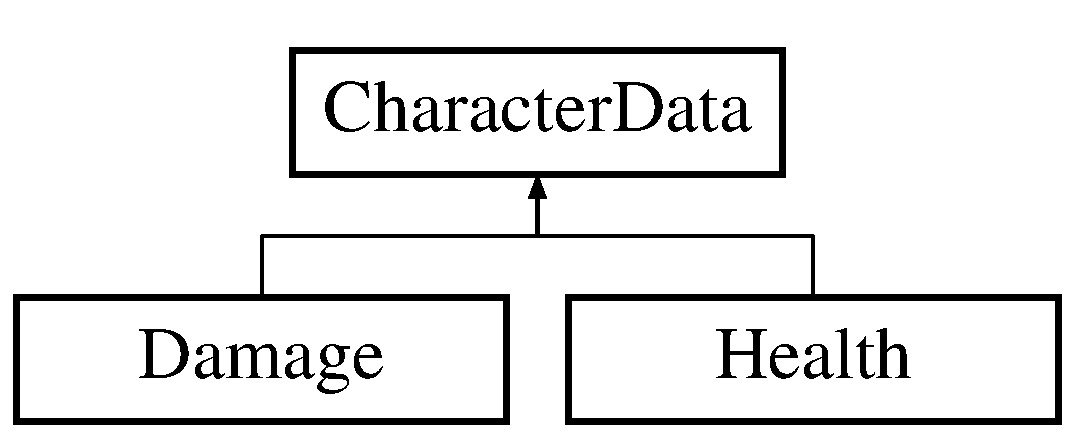
\includegraphics[height=2.000000cm]{struct_character_data}
\end{center}
\end{figure}
\subsection*{Public Member Functions}
\begin{DoxyCompactItemize}
\item 
\hyperlink{struct_character_data_ace49d29c55eeb48f7fd511841df40c27}{Character\-Data} ()
\item 
\hyperlink{struct_character_data_abcb9f0bd43c518b28e02065b171d7551}{Character\-Data} (unsigned long b)
\item 
\hyperlink{struct_character_data_a28743377c793f39f4203ae71a4a40da9}{Character\-Data} (unsigned long b, unsigned m)
\item 
\hyperlink{struct_character_data_a9c4f926d20bfcbeaaf9496791160c09d}{Character\-Data} (const \hyperlink{struct_character_data}{Character\-Data} \&other)
\item 
\hyperlink{struct_character_data_a6e4a98d0dfcffd3155846515a9903900}{Character\-Data} (\hyperlink{struct_character_data}{Character\-Data} \&\&other)
\item 
\hyperlink{struct_character_data}{Character\-Data} \& \hyperlink{struct_character_data_a0118f9a14b08db8bf36870ac1043c780}{operator=} (const \hyperlink{struct_character_data}{Character\-Data} \&rhs)
\item 
\hyperlink{struct_character_data}{Character\-Data} \& \hyperlink{struct_character_data_a8241609b7d0abaf5135fc965234dc1d7}{operator=} (\hyperlink{struct_character_data}{Character\-Data} \&\&rhs)
\item 
bool \hyperlink{struct_character_data_a815d34f2397d83e26a850f7327e121f8}{operator==} (\hyperlink{struct_character_data}{Character\-Data} \&rhs)
\item 
bool \hyperlink{struct_character_data_acc34abfc386287c8c38d0de255aa3442}{operator!=} (\hyperlink{struct_character_data}{Character\-Data} \&rhs)
\item 
bool \hyperlink{struct_character_data_a662008be5f99b06b927ba1def39a12f3}{operator$>$} (\hyperlink{struct_character_data}{Character\-Data} \&rhs)
\item 
bool \hyperlink{struct_character_data_a8531abd07619859ef83ac3ad3e3c3329}{operator$<$} (\hyperlink{struct_character_data}{Character\-Data} \&rhs)
\item 
bool \hyperlink{struct_character_data_a8f31e2a333183cb8c5c5bb2518933ee0}{operator$>$=} (\hyperlink{struct_character_data}{Character\-Data} \&rhs)
\item 
bool \hyperlink{struct_character_data_a8eef34f1395329eb392fb293f7de687d}{operator$<$=} (\hyperlink{struct_character_data}{Character\-Data} \&rhs)
\item 
\hyperlink{struct_character_data}{Character\-Data} \& \hyperlink{struct_character_data_a85313590521d86ff18bfcb6a653919e6}{operator+} (const \hyperlink{struct_character_data}{Character\-Data} \&rhs)
\item 
\hyperlink{struct_character_data}{Character\-Data} \& \hyperlink{struct_character_data_afa94ff26fee5818c3603444600ed37b9}{operator-\/} (const \hyperlink{struct_character_data}{Character\-Data} \&rhs)
\item 
unsigned long \hyperlink{struct_character_data_a65eb0fdcbb3ccab7f1b685df11161a1e}{value} () const 
\item 
unsigned long \hyperlink{struct_character_data_a55c28ca84668020f8e9df060c9e5effc}{operator()} ()
\end{DoxyCompactItemize}
\subsection*{Protected Attributes}
\begin{DoxyCompactItemize}
\item 
unsigned long \hyperlink{struct_character_data_a86c73102954363266a65ee283ff63c02}{base\-Value}
\item 
unsigned int \hyperlink{struct_character_data_adc89389cfd62de262b8fa380703a8705}{modifier}
\end{DoxyCompactItemize}
\subsection*{Friends}
\begin{DoxyCompactItemize}
\item 
ostream \& \hyperlink{struct_character_data_ac3bffef95c1ca2d8be9c0b197dcd383d}{operator$<$$<$} (std\-::ostream \&os, \hyperlink{struct_character_data}{Character\-Data} \&gmd)
\item 
ostream \& \hyperlink{struct_character_data_a662f4fb97ebcbf9be2a543877e6b95ae}{operator$<$$<$} (std\-::ostream \&os, const \hyperlink{struct_character_data}{Character\-Data} \&gmd)
\end{DoxyCompactItemize}


\subsection{Detailed Description}
A parent type that will define the basic functions and members for \hyperlink{struct_damage}{Damage} and \hyperlink{struct_health}{Health} (and other similar data types if we need them) 

Definition at line 25 of file Character\-Data.\-h.



\subsection{Constructor \& Destructor Documentation}
\hypertarget{struct_character_data_ace49d29c55eeb48f7fd511841df40c27}{\index{Character\-Data@{Character\-Data}!Character\-Data@{Character\-Data}}
\index{Character\-Data@{Character\-Data}!CharacterData@{Character\-Data}}
\subsubsection[{Character\-Data}]{\setlength{\rightskip}{0pt plus 5cm}Character\-Data\-::\-Character\-Data (
\begin{DoxyParamCaption}
{}
\end{DoxyParamCaption}
)\hspace{0.3cm}{\ttfamily [inline]}}}\label{struct_character_data_ace49d29c55eeb48f7fd511841df40c27}


Definition at line 34 of file Character\-Data.\-h.

\hypertarget{struct_character_data_abcb9f0bd43c518b28e02065b171d7551}{\index{Character\-Data@{Character\-Data}!Character\-Data@{Character\-Data}}
\index{Character\-Data@{Character\-Data}!CharacterData@{Character\-Data}}
\subsubsection[{Character\-Data}]{\setlength{\rightskip}{0pt plus 5cm}Character\-Data\-::\-Character\-Data (
\begin{DoxyParamCaption}
\item[{unsigned long}]{b}
\end{DoxyParamCaption}
)\hspace{0.3cm}{\ttfamily [inline]}}}\label{struct_character_data_abcb9f0bd43c518b28e02065b171d7551}


Definition at line 38 of file Character\-Data.\-h.

\hypertarget{struct_character_data_a28743377c793f39f4203ae71a4a40da9}{\index{Character\-Data@{Character\-Data}!Character\-Data@{Character\-Data}}
\index{Character\-Data@{Character\-Data}!CharacterData@{Character\-Data}}
\subsubsection[{Character\-Data}]{\setlength{\rightskip}{0pt plus 5cm}Character\-Data\-::\-Character\-Data (
\begin{DoxyParamCaption}
\item[{unsigned long}]{b, }
\item[{unsigned}]{m}
\end{DoxyParamCaption}
)\hspace{0.3cm}{\ttfamily [inline]}}}\label{struct_character_data_a28743377c793f39f4203ae71a4a40da9}


Definition at line 43 of file Character\-Data.\-h.

\hypertarget{struct_character_data_a9c4f926d20bfcbeaaf9496791160c09d}{\index{Character\-Data@{Character\-Data}!Character\-Data@{Character\-Data}}
\index{Character\-Data@{Character\-Data}!CharacterData@{Character\-Data}}
\subsubsection[{Character\-Data}]{\setlength{\rightskip}{0pt plus 5cm}Character\-Data\-::\-Character\-Data (
\begin{DoxyParamCaption}
\item[{const {\bf Character\-Data} \&}]{other}
\end{DoxyParamCaption}
)\hspace{0.3cm}{\ttfamily [inline]}}}\label{struct_character_data_a9c4f926d20bfcbeaaf9496791160c09d}


Definition at line 48 of file Character\-Data.\-h.

\hypertarget{struct_character_data_a6e4a98d0dfcffd3155846515a9903900}{\index{Character\-Data@{Character\-Data}!Character\-Data@{Character\-Data}}
\index{Character\-Data@{Character\-Data}!CharacterData@{Character\-Data}}
\subsubsection[{Character\-Data}]{\setlength{\rightskip}{0pt plus 5cm}Character\-Data\-::\-Character\-Data (
\begin{DoxyParamCaption}
\item[{{\bf Character\-Data} \&\&}]{other}
\end{DoxyParamCaption}
)\hspace{0.3cm}{\ttfamily [inline]}}}\label{struct_character_data_a6e4a98d0dfcffd3155846515a9903900}


Definition at line 52 of file Character\-Data.\-h.



\subsection{Member Function Documentation}
\hypertarget{struct_character_data_acc34abfc386287c8c38d0de255aa3442}{\index{Character\-Data@{Character\-Data}!operator!=@{operator!=}}
\index{operator!=@{operator!=}!CharacterData@{Character\-Data}}
\subsubsection[{operator!=}]{\setlength{\rightskip}{0pt plus 5cm}bool Character\-Data\-::operator!= (
\begin{DoxyParamCaption}
\item[{{\bf Character\-Data} \&}]{rhs}
\end{DoxyParamCaption}
)\hspace{0.3cm}{\ttfamily [inline]}}}\label{struct_character_data_acc34abfc386287c8c38d0de255aa3442}


Definition at line 77 of file Character\-Data.\-h.

\hypertarget{struct_character_data_a55c28ca84668020f8e9df060c9e5effc}{\index{Character\-Data@{Character\-Data}!operator()@{operator()}}
\index{operator()@{operator()}!CharacterData@{Character\-Data}}
\subsubsection[{operator()}]{\setlength{\rightskip}{0pt plus 5cm}unsigned long Character\-Data\-::operator() (
\begin{DoxyParamCaption}
{}
\end{DoxyParamCaption}
)\hspace{0.3cm}{\ttfamily [inline]}}}\label{struct_character_data_a55c28ca84668020f8e9df060c9e5effc}
See \hyperlink{struct_character_data_a65eb0fdcbb3ccab7f1b685df11161a1e}{value()}

\begin{DoxyReturn}{Returns}
The total amount of this \hyperlink{struct_character_data}{Character\-Data} value (e.\-g. \hyperlink{struct_health}{Health} or \hyperlink{struct_damage}{Damage} 
\end{DoxyReturn}


Definition at line 140 of file Character\-Data.\-h.

\hypertarget{struct_character_data_a85313590521d86ff18bfcb6a653919e6}{\index{Character\-Data@{Character\-Data}!operator+@{operator+}}
\index{operator+@{operator+}!CharacterData@{Character\-Data}}
\subsubsection[{operator+}]{\setlength{\rightskip}{0pt plus 5cm}{\bf Character\-Data}\& Character\-Data\-::operator+ (
\begin{DoxyParamCaption}
\item[{const {\bf Character\-Data} \&}]{rhs}
\end{DoxyParamCaption}
)\hspace{0.3cm}{\ttfamily [inline]}}}\label{struct_character_data_a85313590521d86ff18bfcb6a653919e6}


Definition at line 97 of file Character\-Data.\-h.

\hypertarget{struct_character_data_afa94ff26fee5818c3603444600ed37b9}{\index{Character\-Data@{Character\-Data}!operator-\/@{operator-\/}}
\index{operator-\/@{operator-\/}!CharacterData@{Character\-Data}}
\subsubsection[{operator-\/}]{\setlength{\rightskip}{0pt plus 5cm}{\bf Character\-Data}\& Character\-Data\-::operator-\/ (
\begin{DoxyParamCaption}
\item[{const {\bf Character\-Data} \&}]{rhs}
\end{DoxyParamCaption}
)\hspace{0.3cm}{\ttfamily [inline]}}}\label{struct_character_data_afa94ff26fee5818c3603444600ed37b9}


Definition at line 103 of file Character\-Data.\-h.

\hypertarget{struct_character_data_a8531abd07619859ef83ac3ad3e3c3329}{\index{Character\-Data@{Character\-Data}!operator$<$@{operator$<$}}
\index{operator$<$@{operator$<$}!CharacterData@{Character\-Data}}
\subsubsection[{operator$<$}]{\setlength{\rightskip}{0pt plus 5cm}bool Character\-Data\-::operator$<$ (
\begin{DoxyParamCaption}
\item[{{\bf Character\-Data} \&}]{rhs}
\end{DoxyParamCaption}
)\hspace{0.3cm}{\ttfamily [inline]}}}\label{struct_character_data_a8531abd07619859ef83ac3ad3e3c3329}


Definition at line 85 of file Character\-Data.\-h.

\hypertarget{struct_character_data_a8eef34f1395329eb392fb293f7de687d}{\index{Character\-Data@{Character\-Data}!operator$<$=@{operator$<$=}}
\index{operator$<$=@{operator$<$=}!CharacterData@{Character\-Data}}
\subsubsection[{operator$<$=}]{\setlength{\rightskip}{0pt plus 5cm}bool Character\-Data\-::operator$<$= (
\begin{DoxyParamCaption}
\item[{{\bf Character\-Data} \&}]{rhs}
\end{DoxyParamCaption}
)\hspace{0.3cm}{\ttfamily [inline]}}}\label{struct_character_data_a8eef34f1395329eb392fb293f7de687d}


Definition at line 93 of file Character\-Data.\-h.

\hypertarget{struct_character_data_a0118f9a14b08db8bf36870ac1043c780}{\index{Character\-Data@{Character\-Data}!operator=@{operator=}}
\index{operator=@{operator=}!CharacterData@{Character\-Data}}
\subsubsection[{operator=}]{\setlength{\rightskip}{0pt plus 5cm}{\bf Character\-Data}\& Character\-Data\-::operator= (
\begin{DoxyParamCaption}
\item[{const {\bf Character\-Data} \&}]{rhs}
\end{DoxyParamCaption}
)\hspace{0.3cm}{\ttfamily [inline]}}}\label{struct_character_data_a0118f9a14b08db8bf36870ac1043c780}


Definition at line 57 of file Character\-Data.\-h.

\hypertarget{struct_character_data_a8241609b7d0abaf5135fc965234dc1d7}{\index{Character\-Data@{Character\-Data}!operator=@{operator=}}
\index{operator=@{operator=}!CharacterData@{Character\-Data}}
\subsubsection[{operator=}]{\setlength{\rightskip}{0pt plus 5cm}{\bf Character\-Data}\& Character\-Data\-::operator= (
\begin{DoxyParamCaption}
\item[{{\bf Character\-Data} \&\&}]{rhs}
\end{DoxyParamCaption}
)\hspace{0.3cm}{\ttfamily [inline]}}}\label{struct_character_data_a8241609b7d0abaf5135fc965234dc1d7}


Definition at line 65 of file Character\-Data.\-h.

\hypertarget{struct_character_data_a815d34f2397d83e26a850f7327e121f8}{\index{Character\-Data@{Character\-Data}!operator==@{operator==}}
\index{operator==@{operator==}!CharacterData@{Character\-Data}}
\subsubsection[{operator==}]{\setlength{\rightskip}{0pt plus 5cm}bool Character\-Data\-::operator== (
\begin{DoxyParamCaption}
\item[{{\bf Character\-Data} \&}]{rhs}
\end{DoxyParamCaption}
)\hspace{0.3cm}{\ttfamily [inline]}}}\label{struct_character_data_a815d34f2397d83e26a850f7327e121f8}


Definition at line 73 of file Character\-Data.\-h.

\hypertarget{struct_character_data_a662008be5f99b06b927ba1def39a12f3}{\index{Character\-Data@{Character\-Data}!operator$>$@{operator$>$}}
\index{operator$>$@{operator$>$}!CharacterData@{Character\-Data}}
\subsubsection[{operator$>$}]{\setlength{\rightskip}{0pt plus 5cm}bool Character\-Data\-::operator$>$ (
\begin{DoxyParamCaption}
\item[{{\bf Character\-Data} \&}]{rhs}
\end{DoxyParamCaption}
)\hspace{0.3cm}{\ttfamily [inline]}}}\label{struct_character_data_a662008be5f99b06b927ba1def39a12f3}


Definition at line 81 of file Character\-Data.\-h.

\hypertarget{struct_character_data_a8f31e2a333183cb8c5c5bb2518933ee0}{\index{Character\-Data@{Character\-Data}!operator$>$=@{operator$>$=}}
\index{operator$>$=@{operator$>$=}!CharacterData@{Character\-Data}}
\subsubsection[{operator$>$=}]{\setlength{\rightskip}{0pt plus 5cm}bool Character\-Data\-::operator$>$= (
\begin{DoxyParamCaption}
\item[{{\bf Character\-Data} \&}]{rhs}
\end{DoxyParamCaption}
)\hspace{0.3cm}{\ttfamily [inline]}}}\label{struct_character_data_a8f31e2a333183cb8c5c5bb2518933ee0}


Definition at line 89 of file Character\-Data.\-h.

\hypertarget{struct_character_data_a65eb0fdcbb3ccab7f1b685df11161a1e}{\index{Character\-Data@{Character\-Data}!value@{value}}
\index{value@{value}!CharacterData@{Character\-Data}}
\subsubsection[{value}]{\setlength{\rightskip}{0pt plus 5cm}unsigned long Character\-Data\-::value (
\begin{DoxyParamCaption}
{}
\end{DoxyParamCaption}
) const\hspace{0.3cm}{\ttfamily [inline]}}}\label{struct_character_data_a65eb0fdcbb3ccab7f1b685df11161a1e}
\begin{DoxyReturn}{Returns}
The value of this \hyperlink{struct_character_data}{Character\-Data} object (e.\-g. \hyperlink{struct_health}{Health} or \hyperlink{struct_damage}{Damage}) 
\end{DoxyReturn}


Definition at line 131 of file Character\-Data.\-h.



\subsection{Friends And Related Function Documentation}
\hypertarget{struct_character_data_ac3bffef95c1ca2d8be9c0b197dcd383d}{\index{Character\-Data@{Character\-Data}!operator$<$$<$@{operator$<$$<$}}
\index{operator$<$$<$@{operator$<$$<$}!CharacterData@{Character\-Data}}
\subsubsection[{operator$<$$<$}]{\setlength{\rightskip}{0pt plus 5cm}ostream\& operator$<$$<$ (
\begin{DoxyParamCaption}
\item[{std\-::ostream \&}]{os, }
\item[{{\bf Character\-Data} \&}]{gmd}
\end{DoxyParamCaption}
)\hspace{0.3cm}{\ttfamily [friend]}}}\label{struct_character_data_ac3bffef95c1ca2d8be9c0b197dcd383d}
Override the $<$$<$ output stream operator 

Definition at line 113 of file Character\-Data.\-h.

\hypertarget{struct_character_data_a662f4fb97ebcbf9be2a543877e6b95ae}{\index{Character\-Data@{Character\-Data}!operator$<$$<$@{operator$<$$<$}}
\index{operator$<$$<$@{operator$<$$<$}!CharacterData@{Character\-Data}}
\subsubsection[{operator$<$$<$}]{\setlength{\rightskip}{0pt plus 5cm}ostream\& operator$<$$<$ (
\begin{DoxyParamCaption}
\item[{std\-::ostream \&}]{os, }
\item[{const {\bf Character\-Data} \&}]{gmd}
\end{DoxyParamCaption}
)\hspace{0.3cm}{\ttfamily [friend]}}}\label{struct_character_data_a662f4fb97ebcbf9be2a543877e6b95ae}
Override the $<$$<$ output stream operator 

Definition at line 122 of file Character\-Data.\-h.



\subsection{Member Data Documentation}
\hypertarget{struct_character_data_a86c73102954363266a65ee283ff63c02}{\index{Character\-Data@{Character\-Data}!base\-Value@{base\-Value}}
\index{base\-Value@{base\-Value}!CharacterData@{Character\-Data}}
\subsubsection[{base\-Value}]{\setlength{\rightskip}{0pt plus 5cm}unsigned long Character\-Data\-::base\-Value\hspace{0.3cm}{\ttfamily [protected]}}}\label{struct_character_data_a86c73102954363266a65ee283ff63c02}


Definition at line 29 of file Character\-Data.\-h.

\hypertarget{struct_character_data_adc89389cfd62de262b8fa380703a8705}{\index{Character\-Data@{Character\-Data}!modifier@{modifier}}
\index{modifier@{modifier}!CharacterData@{Character\-Data}}
\subsubsection[{modifier}]{\setlength{\rightskip}{0pt plus 5cm}unsigned int Character\-Data\-::modifier\hspace{0.3cm}{\ttfamily [protected]}}}\label{struct_character_data_adc89389cfd62de262b8fa380703a8705}


Definition at line 30 of file Character\-Data.\-h.



The documentation for this struct was generated from the following file\-:\begin{DoxyCompactItemize}
\item 
/\-Volumes/\-O\-S X H\-D\-D/\-Users/\-Adam/\-Developer/\-Sprite\-Fight/\-World/\hyperlink{_character_data_8h}{Character\-Data.\-h}\end{DoxyCompactItemize}

\hypertarget{class_configuration}{\section{Configuration Class Reference}
\label{class_configuration}\index{Configuration@{Configuration}}
}


{\ttfamily \#include $<$Configuration.\-h$>$}

\subsection*{Static Public Member Functions}
\begin{DoxyCompactItemize}
\item 
static void \hyperlink{class_configuration_a83a5078966294216bb61a4dae6d42e0e}{init} ()
\item 
static double \hyperlink{class_configuration_a7e976cf9d781268e3a6cd1afc977f9ce}{global\-Scaling\-Value} ()
\end{DoxyCompactItemize}
\subsection*{Static Public Attributes}
\begin{DoxyCompactItemize}
\item 
static bool \hyperlink{class_configuration_ab18e1dd4f2052c1b7c73ac12ec8c3965}{is\-Init} = false
\end{DoxyCompactItemize}


\subsection{Detailed Description}
This class will mainly be used for overriding default settings, usually based on some form of user input. 

Definition at line 32 of file Configuration.\-h.



\subsection{Member Function Documentation}
\hypertarget{class_configuration_a7e976cf9d781268e3a6cd1afc977f9ce}{\index{Configuration@{Configuration}!global\-Scaling\-Value@{global\-Scaling\-Value}}
\index{global\-Scaling\-Value@{global\-Scaling\-Value}!Configuration@{Configuration}}
\subsubsection[{global\-Scaling\-Value}]{\setlength{\rightskip}{0pt plus 5cm}double Configuration\-::global\-Scaling\-Value (
\begin{DoxyParamCaption}
{}
\end{DoxyParamCaption}
)\hspace{0.3cm}{\ttfamily [static]}}}\label{class_configuration_a7e976cf9d781268e3a6cd1afc977f9ce}
A floating point value used in the calculation of the on-\/screen size of objects. Takes into account that the user can change absolute resolution 

Definition at line 84 of file Configuration.\-cpp.

\hypertarget{class_configuration_a83a5078966294216bb61a4dae6d42e0e}{\index{Configuration@{Configuration}!init@{init}}
\index{init@{init}!Configuration@{Configuration}}
\subsubsection[{init}]{\setlength{\rightskip}{0pt plus 5cm}void Configuration\-::init (
\begin{DoxyParamCaption}
{}
\end{DoxyParamCaption}
)\hspace{0.3cm}{\ttfamily [static]}}}\label{class_configuration_a83a5078966294216bb61a4dae6d42e0e}


Definition at line 58 of file Configuration.\-cpp.



\subsection{Member Data Documentation}
\hypertarget{class_configuration_ab18e1dd4f2052c1b7c73ac12ec8c3965}{\index{Configuration@{Configuration}!is\-Init@{is\-Init}}
\index{is\-Init@{is\-Init}!Configuration@{Configuration}}
\subsubsection[{is\-Init}]{\setlength{\rightskip}{0pt plus 5cm}bool Configuration\-::is\-Init = false\hspace{0.3cm}{\ttfamily [static]}}}\label{class_configuration_ab18e1dd4f2052c1b7c73ac12ec8c3965}


Definition at line 45 of file Configuration.\-h.



The documentation for this class was generated from the following files\-:\begin{DoxyCompactItemize}
\item 
/\-Volumes/\-O\-S X H\-D\-D/\-Users/\-Adam/\-Developer/\-Sprite\-Fight/\-Control/\hyperlink{_configuration_8h}{Configuration.\-h}\item 
/\-Volumes/\-O\-S X H\-D\-D/\-Users/\-Adam/\-Developer/\-Sprite\-Fight/\-Control/\hyperlink{_configuration_8cpp}{Configuration.\-cpp}\end{DoxyCompactItemize}

\hypertarget{class_console_output}{\section{Console\-Output Class Reference}
\label{class_console_output}\index{Console\-Output@{Console\-Output}}
}


{\ttfamily \#include $<$Console\-Output.\-hpp$>$}

\subsection*{Static Public Member Functions}
\begin{DoxyCompactItemize}
\item 
static void \hyperlink{class_console_output_ab1c8015beef82397c02db1f95e04e8f7}{init} ()
\item 
{\footnotesize template$<$typename N $>$ }\\static void \hyperlink{class_console_output_a88787386e1504c6acd4f147a8577ed84}{set\-Output} (const \hyperlink{struct_position}{Position}$<$ N $>$ pos\-\_\-on\-\_\-screen, const char $\ast$str)
\item 
static void \hyperlink{class_console_output_ae7eafee26c6cc9532fbf600804d21a1f}{update} (unsigned int wait\-For\-Microsec)
\item 
static void \hyperlink{class_console_output_a900677fe7791b3198cb35bad848683cd}{exit} ()
\end{DoxyCompactItemize}


\subsection{Detailed Description}


Definition at line 23 of file Console\-Output.\-hpp.



\subsection{Member Function Documentation}
\hypertarget{class_console_output_a900677fe7791b3198cb35bad848683cd}{\index{Console\-Output@{Console\-Output}!exit@{exit}}
\index{exit@{exit}!ConsoleOutput@{Console\-Output}}
\subsubsection[{exit}]{\setlength{\rightskip}{0pt plus 5cm}void Console\-Output\-::exit (
\begin{DoxyParamCaption}
{}
\end{DoxyParamCaption}
)\hspace{0.3cm}{\ttfamily [static]}}}\label{class_console_output_a900677fe7791b3198cb35bad848683cd}


Definition at line 37 of file Console\-Output.\-cpp.

\hypertarget{class_console_output_ab1c8015beef82397c02db1f95e04e8f7}{\index{Console\-Output@{Console\-Output}!init@{init}}
\index{init@{init}!ConsoleOutput@{Console\-Output}}
\subsubsection[{init}]{\setlength{\rightskip}{0pt plus 5cm}void Console\-Output\-::init (
\begin{DoxyParamCaption}
{}
\end{DoxyParamCaption}
)\hspace{0.3cm}{\ttfamily [static]}}}\label{class_console_output_ab1c8015beef82397c02db1f95e04e8f7}


Definition at line 16 of file Console\-Output.\-cpp.

\hypertarget{class_console_output_a88787386e1504c6acd4f147a8577ed84}{\index{Console\-Output@{Console\-Output}!set\-Output@{set\-Output}}
\index{set\-Output@{set\-Output}!ConsoleOutput@{Console\-Output}}
\subsubsection[{set\-Output}]{\setlength{\rightskip}{0pt plus 5cm}template$<$typename N $>$ void Console\-Output\-::set\-Output (
\begin{DoxyParamCaption}
\item[{const {\bf Position}$<$ N $>$}]{pos\-\_\-on\-\_\-screen, }
\item[{const char $\ast$}]{str}
\end{DoxyParamCaption}
)\hspace{0.3cm}{\ttfamily [static]}}}\label{class_console_output_a88787386e1504c6acd4f147a8577ed84}


Definition at line 44 of file Console\-Output.\-hpp.

\hypertarget{class_console_output_ae7eafee26c6cc9532fbf600804d21a1f}{\index{Console\-Output@{Console\-Output}!update@{update}}
\index{update@{update}!ConsoleOutput@{Console\-Output}}
\subsubsection[{update}]{\setlength{\rightskip}{0pt plus 5cm}void Console\-Output\-::update (
\begin{DoxyParamCaption}
\item[{unsigned int}]{wait\-For\-Microsec}
\end{DoxyParamCaption}
)\hspace{0.3cm}{\ttfamily [static]}}}\label{class_console_output_ae7eafee26c6cc9532fbf600804d21a1f}


Definition at line 31 of file Console\-Output.\-cpp.



The documentation for this class was generated from the following files\-:\begin{DoxyCompactItemize}
\item 
/\-Volumes/\-O\-S X H\-D\-D/\-Users/\-Adam/\-Developer/\-Sprite\-Fight/\-Output/\hyperlink{_console_output_8hpp}{Console\-Output.\-hpp}\item 
/\-Volumes/\-O\-S X H\-D\-D/\-Users/\-Adam/\-Developer/\-Sprite\-Fight/\-Output/\hyperlink{_console_output_8cpp}{Console\-Output.\-cpp}\end{DoxyCompactItemize}

\hypertarget{struct_damage}{\section{Damage Struct Reference}
\label{struct_damage}\index{Damage@{Damage}}
}


{\ttfamily \#include $<$Character\-Data.\-h$>$}

Inheritance diagram for Damage\-:\begin{figure}[H]
\begin{center}
\leavevmode
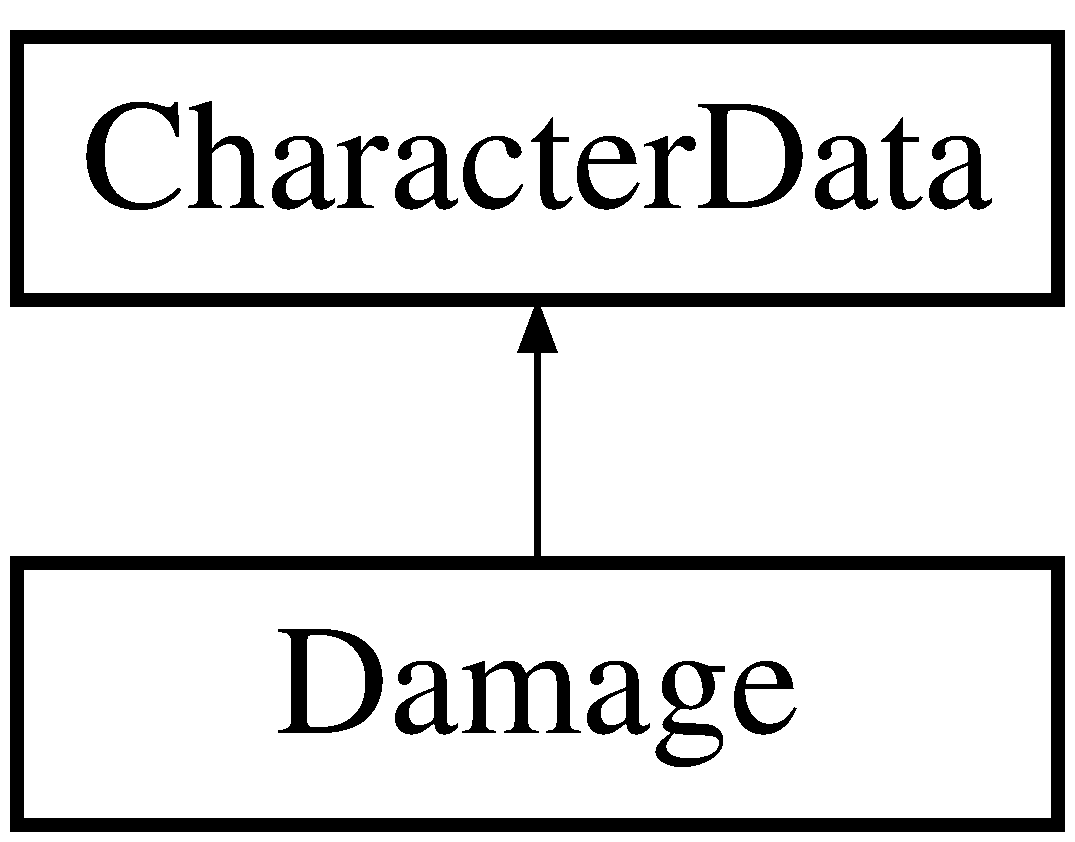
\includegraphics[height=2.000000cm]{struct_damage}
\end{center}
\end{figure}
\subsection*{Public Member Functions}
\begin{DoxyCompactItemize}
\item 
\hyperlink{struct_damage_af71969c367b1b42febfb6ccf8c2d7785}{Damage} ()
\item 
\hyperlink{struct_damage_a2656103f22bbd43950397097289a5b2d}{Damage} (long b)
\item 
\hyperlink{struct_damage_a05b94589f8d332a6a8aa5fe59d646d0b}{Damage} (unsigned long b, unsigned m)
\item 
\hyperlink{struct_damage_a46a26f5c28d52a849ffb457f4a977948}{Damage} (const \hyperlink{struct_damage}{Damage} \&other)
\end{DoxyCompactItemize}
\subsection*{Additional Inherited Members}


\subsection{Detailed Description}
A data structure that will hold damage values 

Definition at line 151 of file Character\-Data.\-h.



\subsection{Constructor \& Destructor Documentation}
\hypertarget{struct_damage_af71969c367b1b42febfb6ccf8c2d7785}{\index{Damage@{Damage}!Damage@{Damage}}
\index{Damage@{Damage}!Damage@{Damage}}
\subsubsection[{Damage}]{\setlength{\rightskip}{0pt plus 5cm}Damage\-::\-Damage (
\begin{DoxyParamCaption}
{}
\end{DoxyParamCaption}
)\hspace{0.3cm}{\ttfamily [inline]}}}\label{struct_damage_af71969c367b1b42febfb6ccf8c2d7785}


Definition at line 155 of file Character\-Data.\-h.

\hypertarget{struct_damage_a2656103f22bbd43950397097289a5b2d}{\index{Damage@{Damage}!Damage@{Damage}}
\index{Damage@{Damage}!Damage@{Damage}}
\subsubsection[{Damage}]{\setlength{\rightskip}{0pt plus 5cm}Damage\-::\-Damage (
\begin{DoxyParamCaption}
\item[{long}]{b}
\end{DoxyParamCaption}
)\hspace{0.3cm}{\ttfamily [inline]}}}\label{struct_damage_a2656103f22bbd43950397097289a5b2d}


Definition at line 158 of file Character\-Data.\-h.

\hypertarget{struct_damage_a05b94589f8d332a6a8aa5fe59d646d0b}{\index{Damage@{Damage}!Damage@{Damage}}
\index{Damage@{Damage}!Damage@{Damage}}
\subsubsection[{Damage}]{\setlength{\rightskip}{0pt plus 5cm}Damage\-::\-Damage (
\begin{DoxyParamCaption}
\item[{unsigned long}]{b, }
\item[{unsigned}]{m}
\end{DoxyParamCaption}
)\hspace{0.3cm}{\ttfamily [inline]}}}\label{struct_damage_a05b94589f8d332a6a8aa5fe59d646d0b}


Definition at line 161 of file Character\-Data.\-h.

\hypertarget{struct_damage_a46a26f5c28d52a849ffb457f4a977948}{\index{Damage@{Damage}!Damage@{Damage}}
\index{Damage@{Damage}!Damage@{Damage}}
\subsubsection[{Damage}]{\setlength{\rightskip}{0pt plus 5cm}Damage\-::\-Damage (
\begin{DoxyParamCaption}
\item[{const {\bf Damage} \&}]{other}
\end{DoxyParamCaption}
)\hspace{0.3cm}{\ttfamily [inline]}}}\label{struct_damage_a46a26f5c28d52a849ffb457f4a977948}


Definition at line 164 of file Character\-Data.\-h.



The documentation for this struct was generated from the following file\-:\begin{DoxyCompactItemize}
\item 
/\-Volumes/\-O\-S X H\-D\-D/\-Users/\-Adam/\-Developer/\-Sprite\-Fight/\-World/\hyperlink{_character_data_8h}{Character\-Data.\-h}\end{DoxyCompactItemize}

\hypertarget{class_debug}{\section{Debug Class Reference}
\label{class_debug}\index{Debug@{Debug}}
}


{\ttfamily \#include $<$Debug.\-h$>$}

Inheritance diagram for Debug\-:\begin{figure}[H]
\begin{center}
\leavevmode
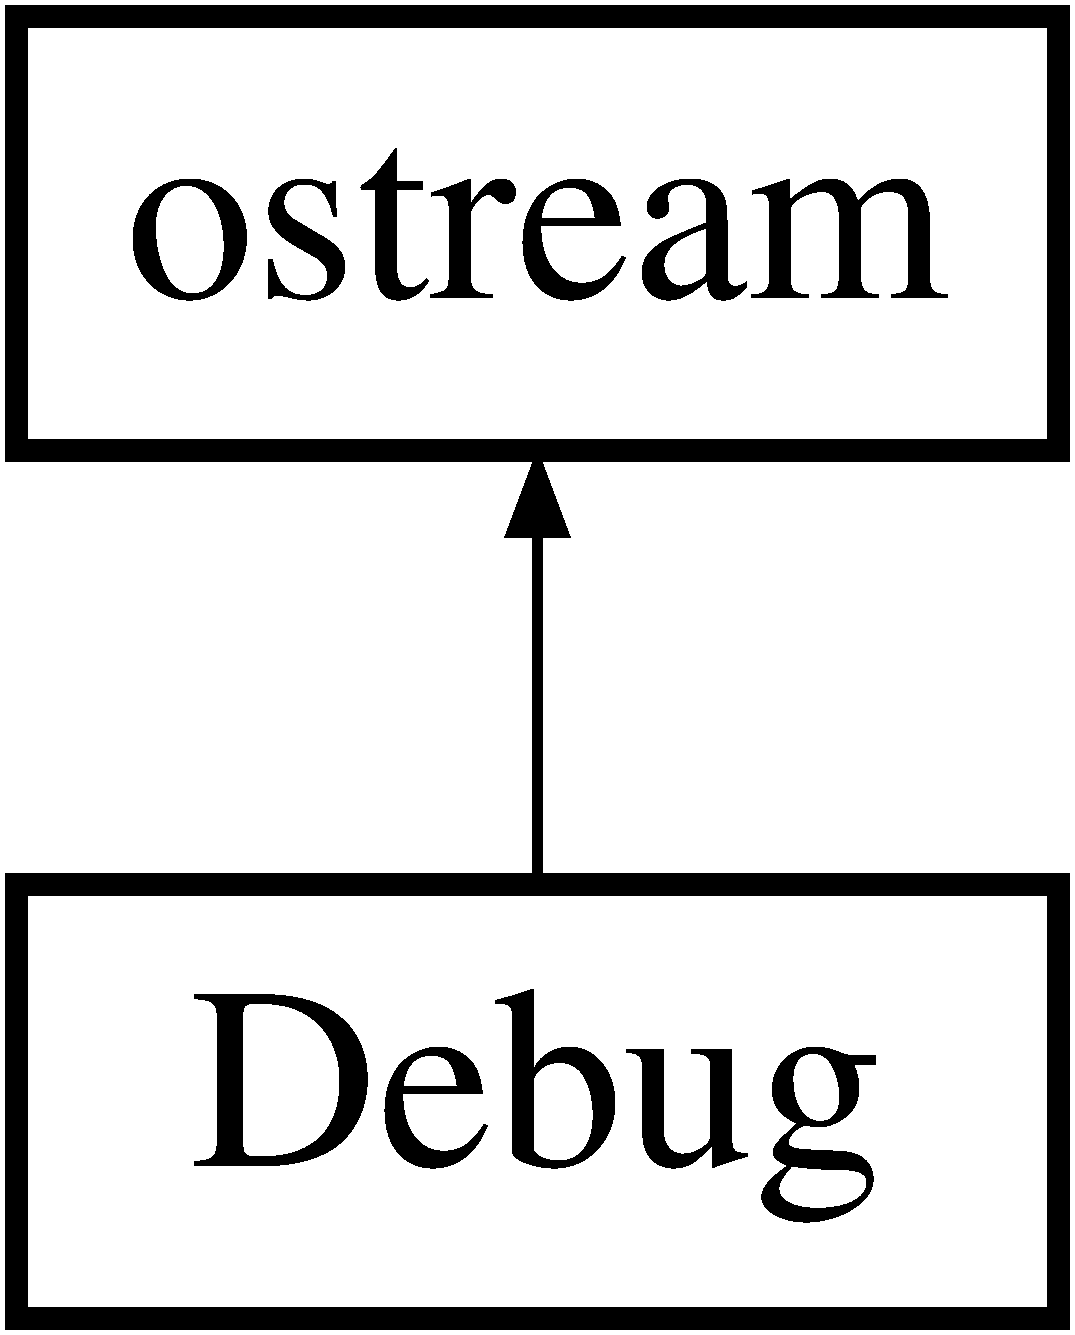
\includegraphics[height=2.000000cm]{class_debug}
\end{center}
\end{figure}
\subsection*{Public Member Functions}
\begin{DoxyCompactItemize}
\item 
\hyperlink{class_debug_ab865c4f64637d49f5fed793824713294}{Debug} (ostream $\ast$\-\_\-out)
\item 
{\footnotesize template$<$typename T $>$ }\\\hyperlink{class_debug}{Debug} \& \hyperlink{class_debug_ad5812b399737871bada69fae4dbba5ec}{operator$<$$<$} (const T \&data)
\item 
\hyperlink{class_debug}{Debug} \& \hyperlink{class_debug_ab9d98c917063f74402ada8ba5298115a}{operator$<$$<$} (std\-::ostream \&($\ast$ptr)(std\-::ostream \&))
\item 
\hyperlink{class_debug}{Debug} \& \hyperlink{class_debug_a6e2f2283770dd91b0a3a2b269ca819b9}{operator$<$$<$} (\hyperlink{class_debug}{Debug} \&($\ast$ptr)(\hyperlink{class_debug}{Debug} \&))
\item 
ostream \& \hyperlink{class_debug_a4e353e9f6c0ec7ea6757d33fe11cd0c2}{get\-\_\-ostream} ()
\end{DoxyCompactItemize}
\subsection*{Static Public Member Functions}
\begin{DoxyCompactItemize}
\item 
static void \hyperlink{class_debug_acd04c0ecba145ac2998cf1c43e7b619b}{init} ()
\end{DoxyCompactItemize}
\subsection*{Static Public Attributes}
\begin{DoxyCompactItemize}
\item 
static \hyperlink{class_debug}{Debug} $\ast$ \hyperlink{class_debug_a1225f6de79fad7fd1cd7b180e139cec1}{debug\-Output} = nullptr
\item 
static unsigned \hyperlink{class_debug_a6ef39adb314b089b4243f544f1d67735}{debug\-Counter} = 0
\end{DoxyCompactItemize}


\subsection{Detailed Description}


Definition at line 21 of file Debug.\-h.



\subsection{Constructor \& Destructor Documentation}
\hypertarget{class_debug_ab865c4f64637d49f5fed793824713294}{\index{Debug@{Debug}!Debug@{Debug}}
\index{Debug@{Debug}!Debug@{Debug}}
\subsubsection[{Debug}]{\setlength{\rightskip}{0pt plus 5cm}Debug\-::\-Debug (
\begin{DoxyParamCaption}
\item[{ostream $\ast$}]{\-\_\-out}
\end{DoxyParamCaption}
)\hspace{0.3cm}{\ttfamily [inline]}}}\label{class_debug_ab865c4f64637d49f5fed793824713294}


Definition at line 34 of file Debug.\-h.



\subsection{Member Function Documentation}
\hypertarget{class_debug_a4e353e9f6c0ec7ea6757d33fe11cd0c2}{\index{Debug@{Debug}!get\-\_\-ostream@{get\-\_\-ostream}}
\index{get\-\_\-ostream@{get\-\_\-ostream}!Debug@{Debug}}
\subsubsection[{get\-\_\-ostream}]{\setlength{\rightskip}{0pt plus 5cm}ostream\& Debug\-::get\-\_\-ostream (
\begin{DoxyParamCaption}
{}
\end{DoxyParamCaption}
)\hspace{0.3cm}{\ttfamily [inline]}}}\label{class_debug_a4e353e9f6c0ec7ea6757d33fe11cd0c2}


Definition at line 63 of file Debug.\-h.

\hypertarget{class_debug_acd04c0ecba145ac2998cf1c43e7b619b}{\index{Debug@{Debug}!init@{init}}
\index{init@{init}!Debug@{Debug}}
\subsubsection[{init}]{\setlength{\rightskip}{0pt plus 5cm}void Debug\-::init (
\begin{DoxyParamCaption}
{}
\end{DoxyParamCaption}
)\hspace{0.3cm}{\ttfamily [static]}}}\label{class_debug_acd04c0ecba145ac2998cf1c43e7b619b}


Definition at line 18 of file Debug.\-cpp.

\hypertarget{class_debug_ad5812b399737871bada69fae4dbba5ec}{\index{Debug@{Debug}!operator$<$$<$@{operator$<$$<$}}
\index{operator$<$$<$@{operator$<$$<$}!Debug@{Debug}}
\subsubsection[{operator$<$$<$}]{\setlength{\rightskip}{0pt plus 5cm}template$<$typename T $>$ {\bf Debug} \& Debug\-::operator$<$$<$ (
\begin{DoxyParamCaption}
\item[{const T \&}]{data}
\end{DoxyParamCaption}
)}}\label{class_debug_ad5812b399737871bada69fae4dbba5ec}


Definition at line 75 of file Debug.\-h.

\hypertarget{class_debug_ab9d98c917063f74402ada8ba5298115a}{\index{Debug@{Debug}!operator$<$$<$@{operator$<$$<$}}
\index{operator$<$$<$@{operator$<$$<$}!Debug@{Debug}}
\subsubsection[{operator$<$$<$}]{\setlength{\rightskip}{0pt plus 5cm}{\bf Debug}\& Debug\-::operator$<$$<$ (
\begin{DoxyParamCaption}
\item[{std\-::ostream \&($\ast$)(std\-::ostream \&)}]{ptr}
\end{DoxyParamCaption}
)\hspace{0.3cm}{\ttfamily [inline]}}}\label{class_debug_ab9d98c917063f74402ada8ba5298115a}


Definition at line 46 of file Debug.\-h.

\hypertarget{class_debug_a6e2f2283770dd91b0a3a2b269ca819b9}{\index{Debug@{Debug}!operator$<$$<$@{operator$<$$<$}}
\index{operator$<$$<$@{operator$<$$<$}!Debug@{Debug}}
\subsubsection[{operator$<$$<$}]{\setlength{\rightskip}{0pt plus 5cm}{\bf Debug}\& Debug\-::operator$<$$<$ (
\begin{DoxyParamCaption}
\item[{{\bf Debug} \&($\ast$)({\bf Debug} \&)}]{ptr}
\end{DoxyParamCaption}
)\hspace{0.3cm}{\ttfamily [inline]}}}\label{class_debug_a6e2f2283770dd91b0a3a2b269ca819b9}


Definition at line 55 of file Debug.\-h.



\subsection{Member Data Documentation}
\hypertarget{class_debug_a6ef39adb314b089b4243f544f1d67735}{\index{Debug@{Debug}!debug\-Counter@{debug\-Counter}}
\index{debug\-Counter@{debug\-Counter}!Debug@{Debug}}
\subsubsection[{debug\-Counter}]{\setlength{\rightskip}{0pt plus 5cm}unsigned Debug\-::debug\-Counter = 0\hspace{0.3cm}{\ttfamily [static]}}}\label{class_debug_a6ef39adb314b089b4243f544f1d67735}


Definition at line 70 of file Debug.\-h.

\hypertarget{class_debug_a1225f6de79fad7fd1cd7b180e139cec1}{\index{Debug@{Debug}!debug\-Output@{debug\-Output}}
\index{debug\-Output@{debug\-Output}!Debug@{Debug}}
\subsubsection[{debug\-Output}]{\setlength{\rightskip}{0pt plus 5cm}{\bf Debug} $\ast$ Debug\-::debug\-Output = nullptr\hspace{0.3cm}{\ttfamily [static]}}}\label{class_debug_a1225f6de79fad7fd1cd7b180e139cec1}


Definition at line 65 of file Debug.\-h.



The documentation for this class was generated from the following files\-:\begin{DoxyCompactItemize}
\item 
/\-Volumes/\-O\-S X H\-D\-D/\-Users/\-Adam/\-Developer/\-Sprite\-Fight/\-Util/\hyperlink{_debug_8h}{Debug.\-h}\item 
/\-Volumes/\-O\-S X H\-D\-D/\-Users/\-Adam/\-Developer/\-Sprite\-Fight/\-Util/\hyperlink{_debug_8cpp}{Debug.\-cpp}\end{DoxyCompactItemize}

\hypertarget{struct_display_data}{\section{Display\-Data Struct Reference}
\label{struct_display_data}\index{Display\-Data@{Display\-Data}}
}


{\ttfamily \#include $<$Display\-Data.\-h$>$}

\subsection*{Static Public Member Functions}
\begin{DoxyCompactItemize}
\item 
static bool \hyperlink{struct_display_data_a44babea5f172f58a4b140fb1c02e68ba}{hi\-D\-P\-I} ()
\item 
static float \hyperlink{struct_display_data_a2a81928e08c2ad29c99c64b6f20146ab}{get\-Display\-Scaling\-Factor} ()
\end{DoxyCompactItemize}


\subsection{Detailed Description}
Holds information about the resolution and scaling of the current display 

Definition at line 15 of file Display\-Data.\-h.



\subsection{Member Function Documentation}
\hypertarget{struct_display_data_a2a81928e08c2ad29c99c64b6f20146ab}{\index{Display\-Data@{Display\-Data}!get\-Display\-Scaling\-Factor@{get\-Display\-Scaling\-Factor}}
\index{get\-Display\-Scaling\-Factor@{get\-Display\-Scaling\-Factor}!DisplayData@{Display\-Data}}
\subsubsection[{get\-Display\-Scaling\-Factor}]{\setlength{\rightskip}{0pt plus 5cm}float Display\-Data\-::get\-Display\-Scaling\-Factor (
\begin{DoxyParamCaption}
{}
\end{DoxyParamCaption}
)\hspace{0.3cm}{\ttfamily [static]}}}\label{struct_display_data_a2a81928e08c2ad29c99c64b6f20146ab}
The display scaling factor. For example, if the system is running in Retina mode, this value will be 2.\-0 

Definition at line 38 of file Display\-Data.\-cpp.

\hypertarget{struct_display_data_a44babea5f172f58a4b140fb1c02e68ba}{\index{Display\-Data@{Display\-Data}!hi\-D\-P\-I@{hi\-D\-P\-I}}
\index{hi\-D\-P\-I@{hi\-D\-P\-I}!DisplayData@{Display\-Data}}
\subsubsection[{hi\-D\-P\-I}]{\setlength{\rightskip}{0pt plus 5cm}bool Display\-Data\-::hi\-D\-P\-I (
\begin{DoxyParamCaption}
{}
\end{DoxyParamCaption}
)\hspace{0.3cm}{\ttfamily [static]}}}\label{struct_display_data_a44babea5f172f58a4b140fb1c02e68ba}
Check if we're running in Retina mode 

Definition at line 26 of file Display\-Data.\-cpp.



The documentation for this struct was generated from the following files\-:\begin{DoxyCompactItemize}
\item 
/\-Volumes/\-O\-S X H\-D\-D/\-Users/\-Adam/\-Developer/\-Sprite\-Fight/\-Output/\hyperlink{_display_data_8h}{Display\-Data.\-h}\item 
/\-Volumes/\-O\-S X H\-D\-D/\-Users/\-Adam/\-Developer/\-Sprite\-Fight/\-Output/\hyperlink{_display_data_8cpp}{Display\-Data.\-cpp}\end{DoxyCompactItemize}

\hypertarget{class_drawing}{\section{Drawing Class Reference}
\label{class_drawing}\index{Drawing@{Drawing}}
}


{\ttfamily \#include $<$Util.\-hpp$>$}

\subsection*{Public Member Functions}
\begin{DoxyCompactItemize}
\item 
{\footnotesize template$<$typename Container $>$ }\\void \hyperlink{class_drawing_a7812f3a85bf7e8ce9e098566d9ae9b40}{draw2\-D\-Representation} (ostream \&write\-To, const Container $\ast$container, char whitespace) const 
\end{DoxyCompactItemize}


\subsection{Detailed Description}


Definition at line 110 of file Util.\-hpp.



\subsection{Member Function Documentation}
\hypertarget{class_drawing_a7812f3a85bf7e8ce9e098566d9ae9b40}{\index{Drawing@{Drawing}!draw2\-D\-Representation@{draw2\-D\-Representation}}
\index{draw2\-D\-Representation@{draw2\-D\-Representation}!Drawing@{Drawing}}
\subsubsection[{draw2\-D\-Representation}]{\setlength{\rightskip}{0pt plus 5cm}template$<$class Container $>$ void Drawing\-::draw2\-D\-Representation (
\begin{DoxyParamCaption}
\item[{ostream \&}]{write\-To, }
\item[{const Container $\ast$}]{container, }
\item[{char}]{whitespace}
\end{DoxyParamCaption}
) const}}\label{class_drawing_a7812f3a85bf7e8ce9e098566d9ae9b40}


Definition at line 131 of file Util.\-hpp.



The documentation for this class was generated from the following file\-:\begin{DoxyCompactItemize}
\item 
/\-Volumes/\-O\-S X H\-D\-D/\-Users/\-Adam/\-Developer/\-Sprite\-Fight/\-Util/\hyperlink{_util_8hpp}{Util.\-hpp}\end{DoxyCompactItemize}

\hypertarget{class_enemy}{\section{Enemy Class Reference}
\label{class_enemy}\index{Enemy@{Enemy}}
}


{\ttfamily \#include $<$Enemy.\-h$>$}

Inheritance diagram for Enemy\-:\begin{figure}[H]
\begin{center}
\leavevmode
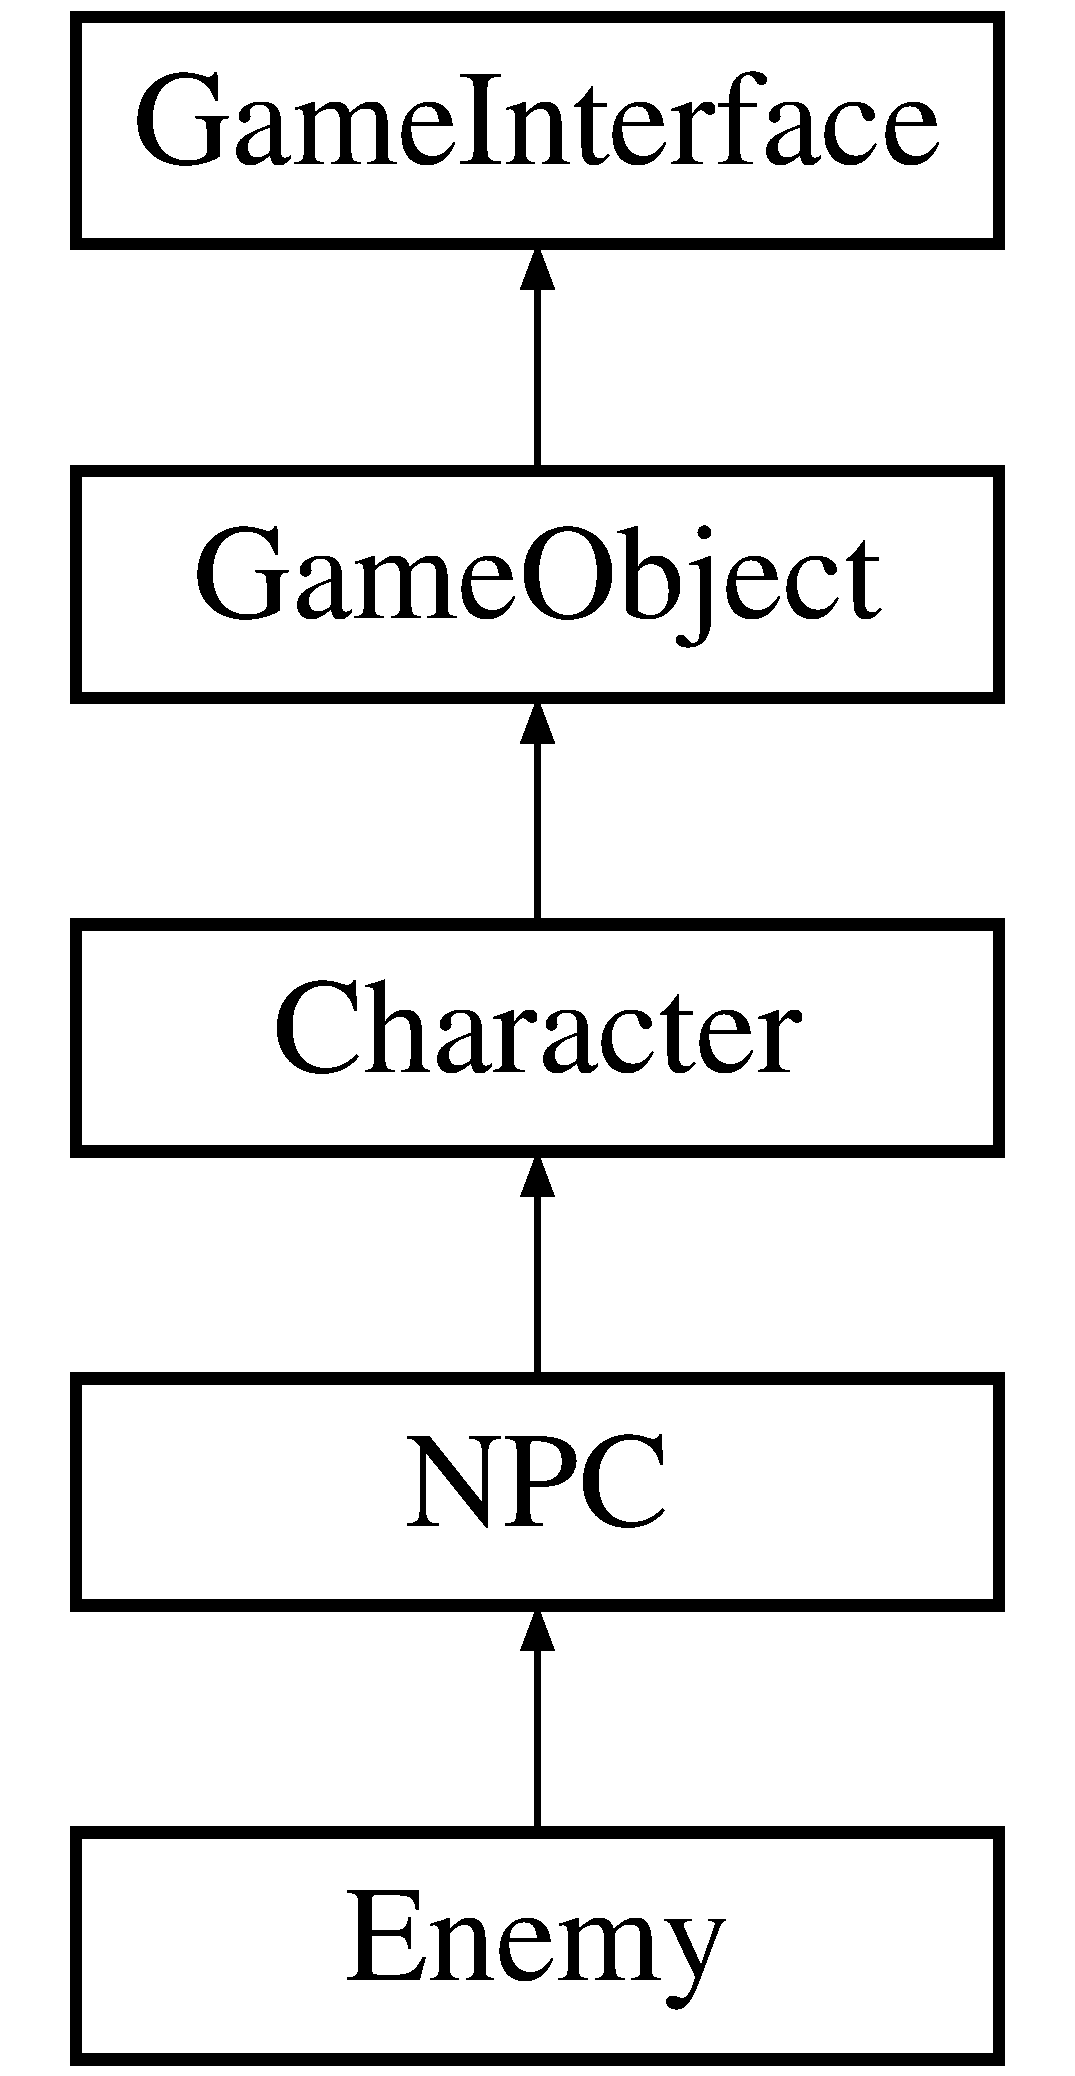
\includegraphics[height=5.000000cm]{class_enemy}
\end{center}
\end{figure}
\subsection*{Public Member Functions}
\begin{DoxyCompactItemize}
\item 
\hyperlink{class_enemy_a94f30d348b6d2840fd71675472ba38dd}{Enemy} ()
\item 
\hyperlink{class_enemy_a6b0c3423456282784e8cc379e956b8a6}{Enemy} (const \hyperlink{struct_asset_file}{Asset\-File} \&image\-File, float \hyperlink{class_game_object_ac4637e122291be2421c851e2a87fb968}{size}, const \hyperlink{struct_position}{Position}$<$ float $>$ \&\hyperlink{class_game_object_a6858e668e7d2c5ded850b952aaacd905}{loc}, string \hyperlink{class_character_a2d423654566d1bf2160fef74bf04cc84}{name}, \hyperlink{_character_data_8h_acbff4d7298e294294555d39178aad448}{Do\-A} \hyperlink{class_character_ac83b99be690bb41b7fae53e9457838c6}{alive}, \hyperlink{_character_data_8h_aacbb008a93d24b04a8779bbdbd8880b5}{Character\-State} \hyperlink{class_character_ac20f1ebda238017ddc245ecdce827037}{state}, unsigned \hyperlink{class_character_ae8c0d82624dc3a171e2c3b42c699151e}{health}, unsigned \hyperlink{class_character_ae6a140637ffe5004179d90a0e04a411b}{damage}, bool monitor\-Velocity, \hyperlink{_character_data_8h_a0e5ce1612c1e71823c97a9cd734de339}{Reaction} \hyperlink{class_character_a579933775b2e4e97465bacb09c4e87f5}{reaction})
\item 
void \hyperlink{class_enemy_acec008d64103ef820006bcbcf9345a2a}{default\-Behaviors} () override
\end{DoxyCompactItemize}
\subsection*{Additional Inherited Members}


\subsection{Detailed Description}


Definition at line 16 of file Enemy.\-h.



\subsection{Constructor \& Destructor Documentation}
\hypertarget{class_enemy_a94f30d348b6d2840fd71675472ba38dd}{\index{Enemy@{Enemy}!Enemy@{Enemy}}
\index{Enemy@{Enemy}!Enemy@{Enemy}}
\subsubsection[{Enemy}]{\setlength{\rightskip}{0pt plus 5cm}Enemy\-::\-Enemy (
\begin{DoxyParamCaption}
{}
\end{DoxyParamCaption}
)\hspace{0.3cm}{\ttfamily [inline]}}}\label{class_enemy_a94f30d348b6d2840fd71675472ba38dd}


Definition at line 22 of file Enemy.\-h.

\hypertarget{class_enemy_a6b0c3423456282784e8cc379e956b8a6}{\index{Enemy@{Enemy}!Enemy@{Enemy}}
\index{Enemy@{Enemy}!Enemy@{Enemy}}
\subsubsection[{Enemy}]{\setlength{\rightskip}{0pt plus 5cm}Enemy\-::\-Enemy (
\begin{DoxyParamCaption}
\item[{const {\bf Asset\-File} \&}]{image\-File, }
\item[{float}]{size, }
\item[{const {\bf Position}$<$ float $>$ \&}]{loc, }
\item[{string}]{name, }
\item[{{\bf Do\-A}}]{alive, }
\item[{{\bf Character\-State}}]{state, }
\item[{unsigned}]{health, }
\item[{unsigned}]{damage, }
\item[{bool}]{monitor\-Velocity, }
\item[{{\bf Reaction}}]{reaction}
\end{DoxyParamCaption}
)\hspace{0.3cm}{\ttfamily [inline]}}}\label{class_enemy_a6b0c3423456282784e8cc379e956b8a6}


Definition at line 24 of file Enemy.\-h.



\subsection{Member Function Documentation}
\hypertarget{class_enemy_acec008d64103ef820006bcbcf9345a2a}{\index{Enemy@{Enemy}!default\-Behaviors@{default\-Behaviors}}
\index{default\-Behaviors@{default\-Behaviors}!Enemy@{Enemy}}
\subsubsection[{default\-Behaviors}]{\setlength{\rightskip}{0pt plus 5cm}void Enemy\-::default\-Behaviors (
\begin{DoxyParamCaption}
{}
\end{DoxyParamCaption}
)\hspace{0.3cm}{\ttfamily [override]}, {\ttfamily [virtual]}}}\label{class_enemy_acec008d64103ef820006bcbcf9345a2a}
Each \hyperlink{class_game_object}{Game\-Object} can implement this to enable its default behaviors to run on a loop on a separate thread 

Reimplemented from \hyperlink{class_character_ac96260f4fd9b68a33919a65bc9da9bca}{Character}.



Definition at line 12 of file Enemy.\-cpp.



The documentation for this class was generated from the following files\-:\begin{DoxyCompactItemize}
\item 
/\-Volumes/\-O\-S X H\-D\-D/\-Users/\-Adam/\-Developer/\-Sprite\-Fight/\-World/\hyperlink{_enemy_8h}{Enemy.\-h}\item 
/\-Volumes/\-O\-S X H\-D\-D/\-Users/\-Adam/\-Developer/\-Sprite\-Fight/\-World/\hyperlink{_enemy_8cpp}{Enemy.\-cpp}\end{DoxyCompactItemize}

\hypertarget{class_event_register}{\section{Event\-Register Class Reference}
\label{class_event_register}\index{Event\-Register@{Event\-Register}}
}


{\ttfamily \#include $<$Input.\-hpp$>$}

Inheritance diagram for Event\-Register\-:\begin{figure}[H]
\begin{center}
\leavevmode
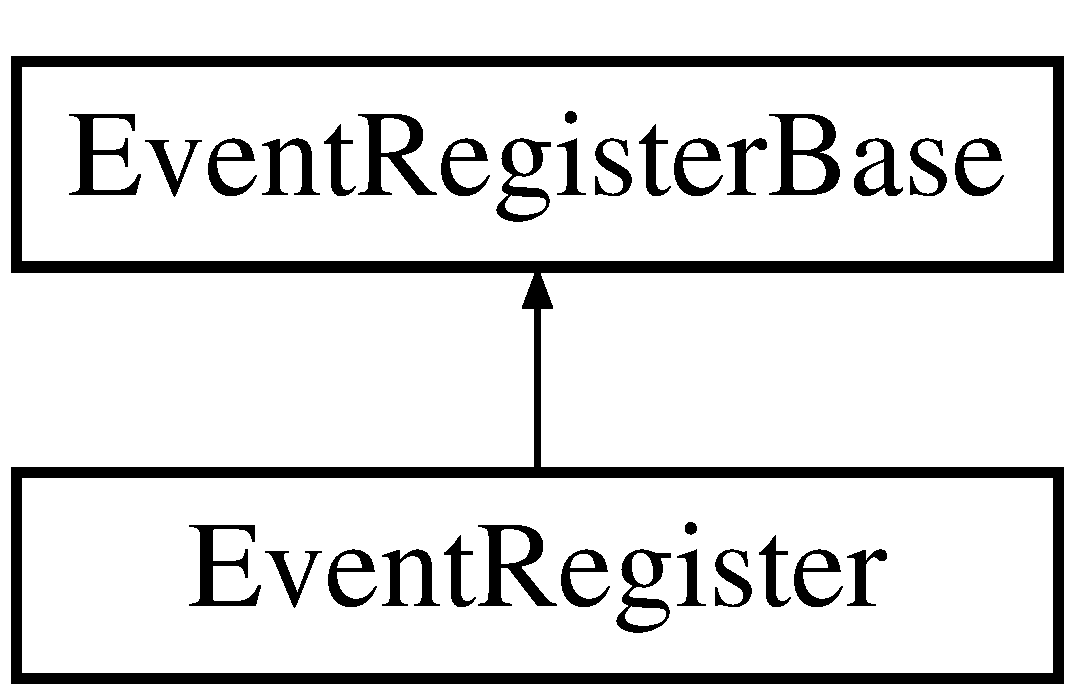
\includegraphics[height=2.000000cm]{class_event_register}
\end{center}
\end{figure}
\subsection*{Public Member Functions}
\begin{DoxyCompactItemize}
\item 
\hyperlink{class_event_register_a41739c6653b17ec40d294591be47e709}{Event\-Register} ()
\item 
\hyperlink{class_event_register_ae5f23b5853832189a422f8bf0f1539ed}{Event\-Register} (const \hyperlink{class_event_register}{Event\-Register} \&other)
\item 
\hyperlink{class_event_register_a4ae5b21f5051b7a8165d3429e33f46b4}{Event\-Register} (\hyperlink{class_event_register}{Event\-Register} \&\&other)
\item 
\hyperlink{class_event_register_a49194d607881335a3a8eb69ecdb636b0}{Event\-Register} (\hyperlink{class_game_interface}{Game\-Interface} $\ast$call\-On, void(Game\-Interface\-::$\ast$cb)(), \hyperlink{_input_8hpp_ae5e40304c43dac2b9c0f1a7e2505e0e7}{Event\-Type} \hyperlink{class_event_register_a0b6153036279b1189d7349d4f97632a9}{event\-Type})
\item 
{\footnotesize template$<$class T $>$ }\\\hyperlink{class_event_register_ae306d8fffaa2290aeee74ec444053ba5}{Event\-Register} (\hyperlink{class_game_interface}{Game\-Interface} $\ast$call\-On, void(Game\-Interface\-::$\ast$cb)(), T $\ast$arg0, \hyperlink{_input_8hpp_ae5e40304c43dac2b9c0f1a7e2505e0e7}{Event\-Type} \hyperlink{class_event_register_a0b6153036279b1189d7349d4f97632a9}{event\-Type})
\item 
\hyperlink{class_event_register_a920b1e5a22a82fee463632f2ebd940bd}{Event\-Register} (function$<$ void(void)$>$ cb, \hyperlink{_input_8hpp_ae5e40304c43dac2b9c0f1a7e2505e0e7}{Event\-Type} \hyperlink{class_event_register_a0b6153036279b1189d7349d4f97632a9}{event\-Type})
\item 
\hyperlink{class_event_register_a2acf491bc76d59b6ae684e6cb5c78519}{$\sim$\-Event\-Register} ()
\item 
void \hyperlink{class_event_register_a452eea8df05259c4c337960f8907003f}{handle\-Event} (const \hyperlink{_input_8hpp_a968dbade547d18c0fc972caf39d984e8}{Event} $\ast$current\-Event)
\end{DoxyCompactItemize}
\subsection*{Protected Attributes}
\begin{DoxyCompactItemize}
\item 
\hyperlink{_input_8hpp_ae5e40304c43dac2b9c0f1a7e2505e0e7}{Event\-Type} \hyperlink{class_event_register_a0b6153036279b1189d7349d4f97632a9}{event\-Type}
\end{DoxyCompactItemize}
\subsection*{Friends}
\begin{DoxyCompactItemize}
\item 
class \hyperlink{class_event_register_a083d5a8d8c2dd3a28d1f55d2965db0ab}{Input\-Controller}
\end{DoxyCompactItemize}
\subsection*{Additional Inherited Members}


\subsection{Detailed Description}
An implementation of \hyperlink{class_event_register_base}{Event\-Register\-Base} with the ability to handle any type of S\-D\-L\-\_\-\-Event. 

Definition at line 117 of file Input.\-hpp.



\subsection{Constructor \& Destructor Documentation}
\hypertarget{class_event_register_a41739c6653b17ec40d294591be47e709}{\index{Event\-Register@{Event\-Register}!Event\-Register@{Event\-Register}}
\index{Event\-Register@{Event\-Register}!EventRegister@{Event\-Register}}
\subsubsection[{Event\-Register}]{\setlength{\rightskip}{0pt plus 5cm}Event\-Register\-::\-Event\-Register (
\begin{DoxyParamCaption}
{}
\end{DoxyParamCaption}
)\hspace{0.3cm}{\ttfamily [inline]}}}\label{class_event_register_a41739c6653b17ec40d294591be47e709}


Definition at line 131 of file Input.\-hpp.

\hypertarget{class_event_register_ae5f23b5853832189a422f8bf0f1539ed}{\index{Event\-Register@{Event\-Register}!Event\-Register@{Event\-Register}}
\index{Event\-Register@{Event\-Register}!EventRegister@{Event\-Register}}
\subsubsection[{Event\-Register}]{\setlength{\rightskip}{0pt plus 5cm}Event\-Register\-::\-Event\-Register (
\begin{DoxyParamCaption}
\item[{const {\bf Event\-Register} \&}]{other}
\end{DoxyParamCaption}
)\hspace{0.3cm}{\ttfamily [inline]}}}\label{class_event_register_ae5f23b5853832189a422f8bf0f1539ed}


Definition at line 133 of file Input.\-hpp.

\hypertarget{class_event_register_a4ae5b21f5051b7a8165d3429e33f46b4}{\index{Event\-Register@{Event\-Register}!Event\-Register@{Event\-Register}}
\index{Event\-Register@{Event\-Register}!EventRegister@{Event\-Register}}
\subsubsection[{Event\-Register}]{\setlength{\rightskip}{0pt plus 5cm}Event\-Register\-::\-Event\-Register (
\begin{DoxyParamCaption}
\item[{{\bf Event\-Register} \&\&}]{other}
\end{DoxyParamCaption}
)\hspace{0.3cm}{\ttfamily [inline]}}}\label{class_event_register_a4ae5b21f5051b7a8165d3429e33f46b4}


Definition at line 137 of file Input.\-hpp.

\hypertarget{class_event_register_a49194d607881335a3a8eb69ecdb636b0}{\index{Event\-Register@{Event\-Register}!Event\-Register@{Event\-Register}}
\index{Event\-Register@{Event\-Register}!EventRegister@{Event\-Register}}
\subsubsection[{Event\-Register}]{\setlength{\rightskip}{0pt plus 5cm}Event\-Register\-::\-Event\-Register (
\begin{DoxyParamCaption}
\item[{{\bf Game\-Interface} $\ast$}]{call\-On, }
\item[{void(Game\-Interface\-::$\ast$)()}]{cb, }
\item[{{\bf Event\-Type}}]{event\-Type}
\end{DoxyParamCaption}
)\hspace{0.3cm}{\ttfamily [inline]}}}\label{class_event_register_a49194d607881335a3a8eb69ecdb636b0}


Definition at line 141 of file Input.\-hpp.

\hypertarget{class_event_register_ae306d8fffaa2290aeee74ec444053ba5}{\index{Event\-Register@{Event\-Register}!Event\-Register@{Event\-Register}}
\index{Event\-Register@{Event\-Register}!EventRegister@{Event\-Register}}
\subsubsection[{Event\-Register}]{\setlength{\rightskip}{0pt plus 5cm}template$<$class T $>$ Event\-Register\-::\-Event\-Register (
\begin{DoxyParamCaption}
\item[{{\bf Game\-Interface} $\ast$}]{call\-On, }
\item[{void(Game\-Interface\-::$\ast$)()}]{cb, }
\item[{T $\ast$}]{arg0, }
\item[{{\bf Event\-Type}}]{event\-Type}
\end{DoxyParamCaption}
)\hspace{0.3cm}{\ttfamily [inline]}}}\label{class_event_register_ae306d8fffaa2290aeee74ec444053ba5}


Definition at line 146 of file Input.\-hpp.

\hypertarget{class_event_register_a920b1e5a22a82fee463632f2ebd940bd}{\index{Event\-Register@{Event\-Register}!Event\-Register@{Event\-Register}}
\index{Event\-Register@{Event\-Register}!EventRegister@{Event\-Register}}
\subsubsection[{Event\-Register}]{\setlength{\rightskip}{0pt plus 5cm}Event\-Register\-::\-Event\-Register (
\begin{DoxyParamCaption}
\item[{function$<$ void(void)$>$}]{cb, }
\item[{{\bf Event\-Type}}]{event\-Type}
\end{DoxyParamCaption}
)\hspace{0.3cm}{\ttfamily [inline]}}}\label{class_event_register_a920b1e5a22a82fee463632f2ebd940bd}


Definition at line 150 of file Input.\-hpp.

\hypertarget{class_event_register_a2acf491bc76d59b6ae684e6cb5c78519}{\index{Event\-Register@{Event\-Register}!$\sim$\-Event\-Register@{$\sim$\-Event\-Register}}
\index{$\sim$\-Event\-Register@{$\sim$\-Event\-Register}!EventRegister@{Event\-Register}}
\subsubsection[{$\sim$\-Event\-Register}]{\setlength{\rightskip}{0pt plus 5cm}Event\-Register\-::$\sim$\-Event\-Register (
\begin{DoxyParamCaption}
{}
\end{DoxyParamCaption}
)\hspace{0.3cm}{\ttfamily [inline]}}}\label{class_event_register_a2acf491bc76d59b6ae684e6cb5c78519}


Definition at line 154 of file Input.\-hpp.



\subsection{Member Function Documentation}
\hypertarget{class_event_register_a452eea8df05259c4c337960f8907003f}{\index{Event\-Register@{Event\-Register}!handle\-Event@{handle\-Event}}
\index{handle\-Event@{handle\-Event}!EventRegister@{Event\-Register}}
\subsubsection[{handle\-Event}]{\setlength{\rightskip}{0pt plus 5cm}void Event\-Register\-::handle\-Event (
\begin{DoxyParamCaption}
\item[{const {\bf Event} $\ast$}]{current\-Event}
\end{DoxyParamCaption}
)}}\label{class_event_register_a452eea8df05259c4c337960f8907003f}


Definition at line 26 of file Input.\-cpp.



\subsection{Friends And Related Function Documentation}
\hypertarget{class_event_register_a083d5a8d8c2dd3a28d1f55d2965db0ab}{\index{Event\-Register@{Event\-Register}!Input\-Controller@{Input\-Controller}}
\index{Input\-Controller@{Input\-Controller}!EventRegister@{Event\-Register}}
\subsubsection[{Input\-Controller}]{\setlength{\rightskip}{0pt plus 5cm}friend class {\bf Input\-Controller}\hspace{0.3cm}{\ttfamily [friend]}}}\label{class_event_register_a083d5a8d8c2dd3a28d1f55d2965db0ab}


Definition at line 126 of file Input.\-hpp.



\subsection{Member Data Documentation}
\hypertarget{class_event_register_a0b6153036279b1189d7349d4f97632a9}{\index{Event\-Register@{Event\-Register}!event\-Type@{event\-Type}}
\index{event\-Type@{event\-Type}!EventRegister@{Event\-Register}}
\subsubsection[{event\-Type}]{\setlength{\rightskip}{0pt plus 5cm}{\bf Event\-Type} Event\-Register\-::event\-Type\hspace{0.3cm}{\ttfamily [protected]}}}\label{class_event_register_a0b6153036279b1189d7349d4f97632a9}
The string representing the keyboard key the client wishes to listen for 

Definition at line 124 of file Input.\-hpp.



The documentation for this class was generated from the following files\-:\begin{DoxyCompactItemize}
\item 
/\-Volumes/\-O\-S X H\-D\-D/\-Users/\-Adam/\-Developer/\-Sprite\-Fight/\-Control/\hyperlink{_input_8hpp}{Input.\-hpp}\item 
/\-Volumes/\-O\-S X H\-D\-D/\-Users/\-Adam/\-Developer/\-Sprite\-Fight/\-Control/\hyperlink{_input_8cpp}{Input.\-cpp}\end{DoxyCompactItemize}

\hypertarget{class_event_register_base}{\section{Event\-Register\-Base Class Reference}
\label{class_event_register_base}\index{Event\-Register\-Base@{Event\-Register\-Base}}
}


{\ttfamily \#include $<$Input.\-hpp$>$}

Inheritance diagram for Event\-Register\-Base\-:\begin{figure}[H]
\begin{center}
\leavevmode
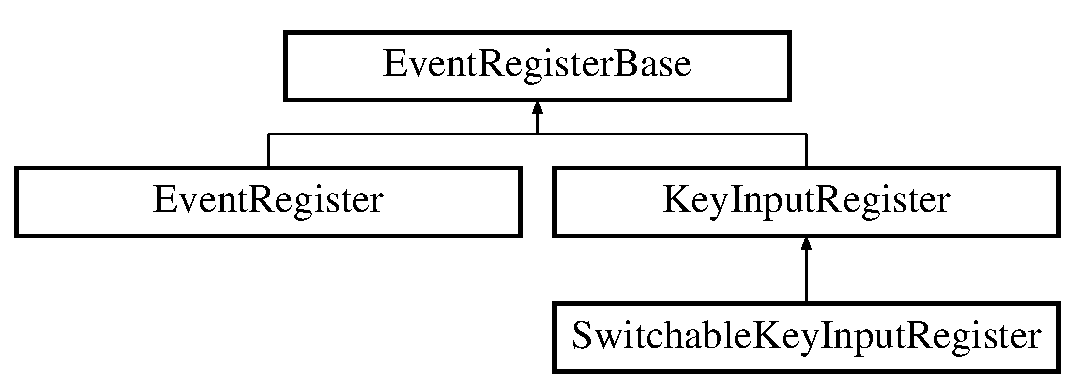
\includegraphics[height=3.000000cm]{class_event_register_base}
\end{center}
\end{figure}
\subsection*{Public Member Functions}
\begin{DoxyCompactItemize}
\item 
void \hyperlink{class_event_register_base_a09c3207daecbf7df0da8e9a9c0d9fa46}{call\-Back} ()
\end{DoxyCompactItemize}
\subsection*{Protected Member Functions}
\begin{DoxyCompactItemize}
\item 
\hyperlink{class_event_register_base_ab73e973655dabe4de4d5f261736a9201}{Event\-Register\-Base} ()
\item 
\hyperlink{class_event_register_base_a63f991f6dd36375b4f845711481d0e8e}{Event\-Register\-Base} (const \hyperlink{class_event_register_base}{Event\-Register\-Base} \&other)
\item 
\hyperlink{class_event_register_base_ae5983e78604cc916282577c7ce0edc18}{Event\-Register\-Base} (\hyperlink{class_event_register_base}{Event\-Register\-Base} \&\&other)
\item 
\hyperlink{class_event_register_base_ad7b93cb60058b038ba9a5e61a3d1e0b5}{Event\-Register\-Base} (\hyperlink{class_game_interface}{Game\-Interface} $\ast$call\-On, void(Game\-Interface\-::$\ast$cb)())
\item 
{\footnotesize template$<$typename T $>$ }\\\hyperlink{class_event_register_base_a945b318dc066bd29c758e9bb78645c25}{Event\-Register\-Base} (\hyperlink{class_game_interface}{Game\-Interface} $\ast$call\-On, void(Game\-Interface\-::$\ast$cb)(), T arg0)
\item 
\hyperlink{class_event_register_base_a85aac264fad1290ad9b4119802401890}{Event\-Register\-Base} (function$<$ void(void)$>$ cb)
\end{DoxyCompactItemize}
\subsection*{Protected Attributes}
\begin{DoxyCompactItemize}
\item 
\hyperlink{class_game_interface}{Game\-Interface} $\ast$ \hyperlink{class_event_register_base_a4747220b6d3bdaadda3adee1ad621d4e}{member\-To\-Call\-On}
\item 
void(Game\-Interface\-::$\ast$ \hyperlink{class_event_register_base_ad0d7c12c7c5c7176a48388cec7e74923}{member\-\_\-call\-Back\-Function} )()
\item 
function$<$ void(void)$>$ \hyperlink{class_event_register_base_a8fcbaadc872f483e42426960e159d4b4}{call\-Back\-Function}
\item 
void $\ast$ \hyperlink{class_event_register_base_ad28e4551bc4710d3a79ff5d5f3f50543}{arg} = nullptr
\end{DoxyCompactItemize}
\subsection*{Friends}
\begin{DoxyCompactItemize}
\item 
class \hyperlink{class_event_register_base_a083d5a8d8c2dd3a28d1f55d2965db0ab}{Input\-Controller}
\end{DoxyCompactItemize}


\subsection{Detailed Description}


Definition at line 37 of file Input.\-hpp.



\subsection{Constructor \& Destructor Documentation}
\hypertarget{class_event_register_base_ab73e973655dabe4de4d5f261736a9201}{\index{Event\-Register\-Base@{Event\-Register\-Base}!Event\-Register\-Base@{Event\-Register\-Base}}
\index{Event\-Register\-Base@{Event\-Register\-Base}!EventRegisterBase@{Event\-Register\-Base}}
\subsubsection[{Event\-Register\-Base}]{\setlength{\rightskip}{0pt plus 5cm}Event\-Register\-Base\-::\-Event\-Register\-Base (
\begin{DoxyParamCaption}
{}
\end{DoxyParamCaption}
)\hspace{0.3cm}{\ttfamily [inline]}, {\ttfamily [protected]}}}\label{class_event_register_base_ab73e973655dabe4de4d5f261736a9201}


Definition at line 73 of file Input.\-hpp.

\hypertarget{class_event_register_base_a63f991f6dd36375b4f845711481d0e8e}{\index{Event\-Register\-Base@{Event\-Register\-Base}!Event\-Register\-Base@{Event\-Register\-Base}}
\index{Event\-Register\-Base@{Event\-Register\-Base}!EventRegisterBase@{Event\-Register\-Base}}
\subsubsection[{Event\-Register\-Base}]{\setlength{\rightskip}{0pt plus 5cm}Event\-Register\-Base\-::\-Event\-Register\-Base (
\begin{DoxyParamCaption}
\item[{const {\bf Event\-Register\-Base} \&}]{other}
\end{DoxyParamCaption}
)\hspace{0.3cm}{\ttfamily [inline]}, {\ttfamily [protected]}}}\label{class_event_register_base_a63f991f6dd36375b4f845711481d0e8e}
Copy constructor 

Definition at line 78 of file Input.\-hpp.

\hypertarget{class_event_register_base_ae5983e78604cc916282577c7ce0edc18}{\index{Event\-Register\-Base@{Event\-Register\-Base}!Event\-Register\-Base@{Event\-Register\-Base}}
\index{Event\-Register\-Base@{Event\-Register\-Base}!EventRegisterBase@{Event\-Register\-Base}}
\subsubsection[{Event\-Register\-Base}]{\setlength{\rightskip}{0pt plus 5cm}Event\-Register\-Base\-::\-Event\-Register\-Base (
\begin{DoxyParamCaption}
\item[{{\bf Event\-Register\-Base} \&\&}]{other}
\end{DoxyParamCaption}
)\hspace{0.3cm}{\ttfamily [inline]}, {\ttfamily [protected]}}}\label{class_event_register_base_ae5983e78604cc916282577c7ce0edc18}
Move constructor 

Definition at line 86 of file Input.\-hpp.

\hypertarget{class_event_register_base_ad7b93cb60058b038ba9a5e61a3d1e0b5}{\index{Event\-Register\-Base@{Event\-Register\-Base}!Event\-Register\-Base@{Event\-Register\-Base}}
\index{Event\-Register\-Base@{Event\-Register\-Base}!EventRegisterBase@{Event\-Register\-Base}}
\subsubsection[{Event\-Register\-Base}]{\setlength{\rightskip}{0pt plus 5cm}Event\-Register\-Base\-::\-Event\-Register\-Base (
\begin{DoxyParamCaption}
\item[{{\bf Game\-Interface} $\ast$}]{call\-On, }
\item[{void(Game\-Interface\-::$\ast$)()}]{cb}
\end{DoxyParamCaption}
)\hspace{0.3cm}{\ttfamily [inline]}, {\ttfamily [protected]}}}\label{class_event_register_base_ad7b93cb60058b038ba9a5e61a3d1e0b5}


Definition at line 91 of file Input.\-hpp.

\hypertarget{class_event_register_base_a945b318dc066bd29c758e9bb78645c25}{\index{Event\-Register\-Base@{Event\-Register\-Base}!Event\-Register\-Base@{Event\-Register\-Base}}
\index{Event\-Register\-Base@{Event\-Register\-Base}!EventRegisterBase@{Event\-Register\-Base}}
\subsubsection[{Event\-Register\-Base}]{\setlength{\rightskip}{0pt plus 5cm}template$<$typename T $>$ Event\-Register\-Base\-::\-Event\-Register\-Base (
\begin{DoxyParamCaption}
\item[{{\bf Game\-Interface} $\ast$}]{call\-On, }
\item[{void(Game\-Interface\-::$\ast$)()}]{cb, }
\item[{T}]{arg0}
\end{DoxyParamCaption}
)\hspace{0.3cm}{\ttfamily [inline]}, {\ttfamily [protected]}}}\label{class_event_register_base_a945b318dc066bd29c758e9bb78645c25}


Definition at line 97 of file Input.\-hpp.

\hypertarget{class_event_register_base_a85aac264fad1290ad9b4119802401890}{\index{Event\-Register\-Base@{Event\-Register\-Base}!Event\-Register\-Base@{Event\-Register\-Base}}
\index{Event\-Register\-Base@{Event\-Register\-Base}!EventRegisterBase@{Event\-Register\-Base}}
\subsubsection[{Event\-Register\-Base}]{\setlength{\rightskip}{0pt plus 5cm}Event\-Register\-Base\-::\-Event\-Register\-Base (
\begin{DoxyParamCaption}
\item[{function$<$ void(void)$>$}]{cb}
\end{DoxyParamCaption}
)\hspace{0.3cm}{\ttfamily [inline]}, {\ttfamily [protected]}}}\label{class_event_register_base_a85aac264fad1290ad9b4119802401890}


Definition at line 103 of file Input.\-hpp.



\subsection{Member Function Documentation}
\hypertarget{class_event_register_base_a09c3207daecbf7df0da8e9a9c0d9fa46}{\index{Event\-Register\-Base@{Event\-Register\-Base}!call\-Back@{call\-Back}}
\index{call\-Back@{call\-Back}!EventRegisterBase@{Event\-Register\-Base}}
\subsubsection[{call\-Back}]{\setlength{\rightskip}{0pt plus 5cm}void Event\-Register\-Base\-::call\-Back (
\begin{DoxyParamCaption}
{}
\end{DoxyParamCaption}
)}}\label{class_event_register_base_a09c3207daecbf7df0da8e9a9c0d9fa46}


Definition at line 15 of file Input.\-cpp.



\subsection{Friends And Related Function Documentation}
\hypertarget{class_event_register_base_a083d5a8d8c2dd3a28d1f55d2965db0ab}{\index{Event\-Register\-Base@{Event\-Register\-Base}!Input\-Controller@{Input\-Controller}}
\index{Input\-Controller@{Input\-Controller}!EventRegisterBase@{Event\-Register\-Base}}
\subsubsection[{Input\-Controller}]{\setlength{\rightskip}{0pt plus 5cm}friend class {\bf Input\-Controller}\hspace{0.3cm}{\ttfamily [friend]}}}\label{class_event_register_base_a083d5a8d8c2dd3a28d1f55d2965db0ab}


Definition at line 71 of file Input.\-hpp.



\subsection{Member Data Documentation}
\hypertarget{class_event_register_base_ad28e4551bc4710d3a79ff5d5f3f50543}{\index{Event\-Register\-Base@{Event\-Register\-Base}!arg@{arg}}
\index{arg@{arg}!EventRegisterBase@{Event\-Register\-Base}}
\subsubsection[{arg}]{\setlength{\rightskip}{0pt plus 5cm}void$\ast$ Event\-Register\-Base\-::arg = nullptr\hspace{0.3cm}{\ttfamily [protected]}}}\label{class_event_register_base_ad28e4551bc4710d3a79ff5d5f3f50543}
In the rare case that our callback function takes an argument, we will use arg to store it 

Definition at line 69 of file Input.\-hpp.

\hypertarget{class_event_register_base_a8fcbaadc872f483e42426960e159d4b4}{\index{Event\-Register\-Base@{Event\-Register\-Base}!call\-Back\-Function@{call\-Back\-Function}}
\index{call\-Back\-Function@{call\-Back\-Function}!EventRegisterBase@{Event\-Register\-Base}}
\subsubsection[{call\-Back\-Function}]{\setlength{\rightskip}{0pt plus 5cm}function$<$void (void)$>$ Event\-Register\-Base\-::call\-Back\-Function\hspace{0.3cm}{\ttfamily [protected]}}}\label{class_event_register_base_a8fcbaadc872f483e42426960e159d4b4}
A pointer to the function to be called when the requested keyboard input is detected. This variable points to static or global functions (member\-\_\-call\-On should be a nullptr in any \hyperlink{class_event_register_base}{Event\-Register\-Base} where a call\-Back\-Fn, and not a member\-\_\-call\-Back\-Fn, is held) 

Definition at line 63 of file Input.\-hpp.

\hypertarget{class_event_register_base_ad0d7c12c7c5c7176a48388cec7e74923}{\index{Event\-Register\-Base@{Event\-Register\-Base}!member\-\_\-call\-Back\-Function@{member\-\_\-call\-Back\-Function}}
\index{member\-\_\-call\-Back\-Function@{member\-\_\-call\-Back\-Function}!EventRegisterBase@{Event\-Register\-Base}}
\subsubsection[{member\-\_\-call\-Back\-Function}]{\setlength{\rightskip}{0pt plus 5cm}void(Game\-Interface\-::$\ast$ Event\-Register\-Base\-::member\-\_\-call\-Back\-Function)()\hspace{0.3cm}{\ttfamily [protected]}}}\label{class_event_register_base_ad0d7c12c7c5c7176a48388cec7e74923}
A pointer to the function to be called when the requested keyboard input is detected. This variable holds pointers to member functions 

Definition at line 52 of file Input.\-hpp.

\hypertarget{class_event_register_base_a4747220b6d3bdaadda3adee1ad621d4e}{\index{Event\-Register\-Base@{Event\-Register\-Base}!member\-To\-Call\-On@{member\-To\-Call\-On}}
\index{member\-To\-Call\-On@{member\-To\-Call\-On}!EventRegisterBase@{Event\-Register\-Base}}
\subsubsection[{member\-To\-Call\-On}]{\setlength{\rightskip}{0pt plus 5cm}{\bf Game\-Interface}$\ast$ Event\-Register\-Base\-::member\-To\-Call\-On\hspace{0.3cm}{\ttfamily [protected]}}}\label{class_event_register_base_a4747220b6d3bdaadda3adee1ad621d4e}
See member\-\_\-call\-Back\-Function. 

Definition at line 45 of file Input.\-hpp.



The documentation for this class was generated from the following files\-:\begin{DoxyCompactItemize}
\item 
/\-Volumes/\-O\-S X H\-D\-D/\-Users/\-Adam/\-Developer/\-Sprite\-Fight/\-Control/\hyperlink{_input_8hpp}{Input.\-hpp}\item 
/\-Volumes/\-O\-S X H\-D\-D/\-Users/\-Adam/\-Developer/\-Sprite\-Fight/\-Control/\hyperlink{_input_8cpp}{Input.\-cpp}\end{DoxyCompactItemize}

\hypertarget{class_fast_rand}{\section{Fast\-Rand$<$ N $>$ Class Template Reference}
\label{class_fast_rand}\index{Fast\-Rand$<$ N $>$@{Fast\-Rand$<$ N $>$}}
}


{\ttfamily \#include $<$Game\-Random.\-hpp$>$}

\subsection*{Public Member Functions}
\begin{DoxyCompactItemize}
\item 
\hyperlink{class_fast_rand_a1b2acd69df1f8ebd670a133186042be4}{Fast\-Rand} (N \-\_\-min, N \-\_\-max)
\item 
\hyperlink{class_fast_rand_a51550e21d1aa8f2e4d92cac8c7466aac}{Fast\-Rand} (const \hyperlink{class_fast_rand}{Fast\-Rand}$<$ N $>$ \&other)
\item 
\hyperlink{class_fast_rand}{Fast\-Rand} \& \hyperlink{class_fast_rand_aed5b803f4e26008d1b133d7181b626ff}{operator=} (const \hyperlink{class_fast_rand}{Fast\-Rand}$<$ N $>$ \&rhs)
\item 
\hyperlink{class_fast_rand_a4acb58985ef91f01b3cb35b0aef2c5ee}{$\sim$\-Fast\-Rand} ()
\item 
N \hyperlink{class_fast_rand_a69ad4de951e5150cbde4b0775f4c029a}{next\-Value} ()
\item 
N \hyperlink{class_fast_rand_ad072e7031fed3100e5852d9e699fec53}{next\-Value} (N \hyperlink{class_fast_rand_a7041d4ec9e4da25457fe86bada8bca49}{minimum}, N \hyperlink{class_fast_rand_aaee674d6363b30ae014073e23e3b2746}{maximum})
\item 
{\footnotesize template$<$typename R $>$ }\\R \hyperlink{class_fast_rand_aae13cb1cd4178cf1cc7f6823de6110aa}{next\-Value} (R \-\_\-min, R \-\_\-max)
\item 
N \hyperlink{class_fast_rand_abc8b63cf6e5430753bcb73d83535d62f}{operator()} ()
\item 
N \hyperlink{class_fast_rand_a2c3b9991bdf5a067f42f0390571b0ddc}{operator()} (N \hyperlink{class_fast_rand_a7041d4ec9e4da25457fe86bada8bca49}{minimum}, N \hyperlink{class_fast_rand_aaee674d6363b30ae014073e23e3b2746}{maximum})
\end{DoxyCompactItemize}
\subsection*{Static Public Attributes}
\begin{DoxyCompactItemize}
\item 
static \hyperlink{class_fast_rand}{Fast\-Rand} \hyperlink{class_fast_rand_ae6756973a197860a27487b65dee1fad0}{default\-Random}
\item 
static \hyperlink{class_fast_rand}{Fast\-Rand} $\ast$ \hyperlink{class_fast_rand_aba6b711ca110b6e3ffa5aef1048cfa9b}{rand\-Position\-Setter} = \hyperlink{class_fast_rand_a32428bea0e468c24ad88e70ceac45617}{init\-Rand\-Pos\-Setter}()
\end{DoxyCompactItemize}
\subsection*{Static Protected Member Functions}
\begin{DoxyCompactItemize}
\item 
static \hyperlink{class_fast_rand}{Fast\-Rand} $\ast$ \hyperlink{class_fast_rand_a32428bea0e468c24ad88e70ceac45617}{init\-Rand\-Pos\-Setter} ()
\end{DoxyCompactItemize}
\subsection*{Protected Attributes}
\begin{DoxyCompactItemize}
\item 
std\-::random\-\_\-device \hyperlink{class_fast_rand_a101185e54f4a2a60a3179a8524c3b8a9}{dev}
\item 
std\-::uniform\-\_\-int\-\_\-distribution$<$ N $>$ \hyperlink{class_fast_rand_a0b39a2388a6512acb59dfba2c9f19ace}{dist}
\item 
std\-::default\-\_\-random\-\_\-engine \hyperlink{class_fast_rand_a8f87664883d9d0567615b169e99bcec5}{rndm} \{\hyperlink{class_fast_rand_a101185e54f4a2a60a3179a8524c3b8a9}{dev}()\}
\item 
N \hyperlink{class_fast_rand_a7041d4ec9e4da25457fe86bada8bca49}{minimum}
\item 
N \hyperlink{class_fast_rand_aaee674d6363b30ae014073e23e3b2746}{maximum}
\end{DoxyCompactItemize}


\subsection{Detailed Description}
\subsubsection*{template$<$typename N$>$class Fast\-Rand$<$ N $>$}



Definition at line 22 of file Game\-Random.\-hpp.



\subsection{Constructor \& Destructor Documentation}
\hypertarget{class_fast_rand_a1b2acd69df1f8ebd670a133186042be4}{\index{Fast\-Rand@{Fast\-Rand}!Fast\-Rand@{Fast\-Rand}}
\index{Fast\-Rand@{Fast\-Rand}!FastRand@{Fast\-Rand}}
\subsubsection[{Fast\-Rand}]{\setlength{\rightskip}{0pt plus 5cm}template$<$typename N$>$ {\bf Fast\-Rand}$<$ N $>$\-::{\bf Fast\-Rand} (
\begin{DoxyParamCaption}
\item[{N}]{\-\_\-min, }
\item[{N}]{\-\_\-max}
\end{DoxyParamCaption}
)}}\label{class_fast_rand_a1b2acd69df1f8ebd670a133186042be4}


Definition at line 92 of file Game\-Random.\-hpp.

\hypertarget{class_fast_rand_a51550e21d1aa8f2e4d92cac8c7466aac}{\index{Fast\-Rand@{Fast\-Rand}!Fast\-Rand@{Fast\-Rand}}
\index{Fast\-Rand@{Fast\-Rand}!FastRand@{Fast\-Rand}}
\subsubsection[{Fast\-Rand}]{\setlength{\rightskip}{0pt plus 5cm}template$<$typename N$>$ {\bf Fast\-Rand}$<$ N $>$\-::{\bf Fast\-Rand} (
\begin{DoxyParamCaption}
\item[{const {\bf Fast\-Rand}$<$ N $>$ \&}]{other}
\end{DoxyParamCaption}
)}}\label{class_fast_rand_a51550e21d1aa8f2e4d92cac8c7466aac}


Definition at line 102 of file Game\-Random.\-hpp.

\hypertarget{class_fast_rand_a4acb58985ef91f01b3cb35b0aef2c5ee}{\index{Fast\-Rand@{Fast\-Rand}!$\sim$\-Fast\-Rand@{$\sim$\-Fast\-Rand}}
\index{$\sim$\-Fast\-Rand@{$\sim$\-Fast\-Rand}!FastRand@{Fast\-Rand}}
\subsubsection[{$\sim$\-Fast\-Rand}]{\setlength{\rightskip}{0pt plus 5cm}template$<$typename N $>$ {\bf Fast\-Rand}$<$ N $>$\-::$\sim${\bf Fast\-Rand} (
\begin{DoxyParamCaption}
{}
\end{DoxyParamCaption}
)}}\label{class_fast_rand_a4acb58985ef91f01b3cb35b0aef2c5ee}


Definition at line 110 of file Game\-Random.\-hpp.



\subsection{Member Function Documentation}
\hypertarget{class_fast_rand_a32428bea0e468c24ad88e70ceac45617}{\index{Fast\-Rand@{Fast\-Rand}!init\-Rand\-Pos\-Setter@{init\-Rand\-Pos\-Setter}}
\index{init\-Rand\-Pos\-Setter@{init\-Rand\-Pos\-Setter}!FastRand@{Fast\-Rand}}
\subsubsection[{init\-Rand\-Pos\-Setter}]{\setlength{\rightskip}{0pt plus 5cm}template$<$typename N $>$ {\bf Fast\-Rand}$<$ N $>$ $\ast$ {\bf Fast\-Rand}$<$ N $>$\-::init\-Rand\-Pos\-Setter (
\begin{DoxyParamCaption}
{}
\end{DoxyParamCaption}
)\hspace{0.3cm}{\ttfamily [static]}, {\ttfamily [protected]}}}\label{class_fast_rand_a32428bea0e468c24ad88e70ceac45617}


Definition at line 155 of file Game\-Random.\-hpp.

\hypertarget{class_fast_rand_a69ad4de951e5150cbde4b0775f4c029a}{\index{Fast\-Rand@{Fast\-Rand}!next\-Value@{next\-Value}}
\index{next\-Value@{next\-Value}!FastRand@{Fast\-Rand}}
\subsubsection[{next\-Value}]{\setlength{\rightskip}{0pt plus 5cm}template$<$typename N $>$ N {\bf Fast\-Rand}$<$ N $>$\-::next\-Value (
\begin{DoxyParamCaption}
{}
\end{DoxyParamCaption}
)}}\label{class_fast_rand_a69ad4de951e5150cbde4b0775f4c029a}


Definition at line 124 of file Game\-Random.\-hpp.

\hypertarget{class_fast_rand_ad072e7031fed3100e5852d9e699fec53}{\index{Fast\-Rand@{Fast\-Rand}!next\-Value@{next\-Value}}
\index{next\-Value@{next\-Value}!FastRand@{Fast\-Rand}}
\subsubsection[{next\-Value}]{\setlength{\rightskip}{0pt plus 5cm}template$<$typename N$>$ N {\bf Fast\-Rand}$<$ N $>$\-::next\-Value (
\begin{DoxyParamCaption}
\item[{N}]{minimum, }
\item[{N}]{maximum}
\end{DoxyParamCaption}
)}}\label{class_fast_rand_ad072e7031fed3100e5852d9e699fec53}


Definition at line 129 of file Game\-Random.\-hpp.

\hypertarget{class_fast_rand_aae13cb1cd4178cf1cc7f6823de6110aa}{\index{Fast\-Rand@{Fast\-Rand}!next\-Value@{next\-Value}}
\index{next\-Value@{next\-Value}!FastRand@{Fast\-Rand}}
\subsubsection[{next\-Value}]{\setlength{\rightskip}{0pt plus 5cm}template$<$typename N $>$ template$<$typename R $>$ R {\bf Fast\-Rand}$<$ N $>$\-::next\-Value (
\begin{DoxyParamCaption}
\item[{R}]{\-\_\-min, }
\item[{R}]{\-\_\-max}
\end{DoxyParamCaption}
)}}\label{class_fast_rand_aae13cb1cd4178cf1cc7f6823de6110aa}


Definition at line 146 of file Game\-Random.\-hpp.

\hypertarget{class_fast_rand_abc8b63cf6e5430753bcb73d83535d62f}{\index{Fast\-Rand@{Fast\-Rand}!operator()@{operator()}}
\index{operator()@{operator()}!FastRand@{Fast\-Rand}}
\subsubsection[{operator()}]{\setlength{\rightskip}{0pt plus 5cm}template$<$typename N $>$ N {\bf Fast\-Rand}$<$ N $>$\-::operator() (
\begin{DoxyParamCaption}
{}
\end{DoxyParamCaption}
)}}\label{class_fast_rand_abc8b63cf6e5430753bcb73d83535d62f}


Definition at line 135 of file Game\-Random.\-hpp.

\hypertarget{class_fast_rand_a2c3b9991bdf5a067f42f0390571b0ddc}{\index{Fast\-Rand@{Fast\-Rand}!operator()@{operator()}}
\index{operator()@{operator()}!FastRand@{Fast\-Rand}}
\subsubsection[{operator()}]{\setlength{\rightskip}{0pt plus 5cm}template$<$typename N$>$ N {\bf Fast\-Rand}$<$ N $>$\-::operator() (
\begin{DoxyParamCaption}
\item[{N}]{minimum, }
\item[{N}]{maximum}
\end{DoxyParamCaption}
)}}\label{class_fast_rand_a2c3b9991bdf5a067f42f0390571b0ddc}


Definition at line 140 of file Game\-Random.\-hpp.

\hypertarget{class_fast_rand_aed5b803f4e26008d1b133d7181b626ff}{\index{Fast\-Rand@{Fast\-Rand}!operator=@{operator=}}
\index{operator=@{operator=}!FastRand@{Fast\-Rand}}
\subsubsection[{operator=}]{\setlength{\rightskip}{0pt plus 5cm}template$<$typename N$>$ {\bf Fast\-Rand}$<$ N $>$ \& {\bf Fast\-Rand}$<$ N $>$\-::operator= (
\begin{DoxyParamCaption}
\item[{const {\bf Fast\-Rand}$<$ N $>$ \&}]{rhs}
\end{DoxyParamCaption}
)}}\label{class_fast_rand_aed5b803f4e26008d1b133d7181b626ff}


Definition at line 113 of file Game\-Random.\-hpp.



\subsection{Member Data Documentation}
\hypertarget{class_fast_rand_ae6756973a197860a27487b65dee1fad0}{\index{Fast\-Rand@{Fast\-Rand}!default\-Random@{default\-Random}}
\index{default\-Random@{default\-Random}!FastRand@{Fast\-Rand}}
\subsubsection[{default\-Random}]{\setlength{\rightskip}{0pt plus 5cm}template$<$typename N$>$ {\bf Fast\-Rand}$<$ N $>$ {\bf Fast\-Rand}$<$ N $>$\-::default\-Random\hspace{0.3cm}{\ttfamily [static]}}}\label{class_fast_rand_ae6756973a197860a27487b65dee1fad0}


Definition at line 43 of file Game\-Random.\-hpp.

\hypertarget{class_fast_rand_a101185e54f4a2a60a3179a8524c3b8a9}{\index{Fast\-Rand@{Fast\-Rand}!dev@{dev}}
\index{dev@{dev}!FastRand@{Fast\-Rand}}
\subsubsection[{dev}]{\setlength{\rightskip}{0pt plus 5cm}template$<$typename N$>$ std\-::random\-\_\-device {\bf Fast\-Rand}$<$ N $>$\-::dev\hspace{0.3cm}{\ttfamily [protected]}}}\label{class_fast_rand_a101185e54f4a2a60a3179a8524c3b8a9}


Definition at line 26 of file Game\-Random.\-hpp.

\hypertarget{class_fast_rand_a0b39a2388a6512acb59dfba2c9f19ace}{\index{Fast\-Rand@{Fast\-Rand}!dist@{dist}}
\index{dist@{dist}!FastRand@{Fast\-Rand}}
\subsubsection[{dist}]{\setlength{\rightskip}{0pt plus 5cm}template$<$typename N$>$ std\-::uniform\-\_\-int\-\_\-distribution$<$N$>$ {\bf Fast\-Rand}$<$ N $>$\-::dist\hspace{0.3cm}{\ttfamily [protected]}}}\label{class_fast_rand_a0b39a2388a6512acb59dfba2c9f19ace}


Definition at line 27 of file Game\-Random.\-hpp.

\hypertarget{class_fast_rand_aaee674d6363b30ae014073e23e3b2746}{\index{Fast\-Rand@{Fast\-Rand}!maximum@{maximum}}
\index{maximum@{maximum}!FastRand@{Fast\-Rand}}
\subsubsection[{maximum}]{\setlength{\rightskip}{0pt plus 5cm}template$<$typename N$>$ N {\bf Fast\-Rand}$<$ N $>$\-::maximum\hspace{0.3cm}{\ttfamily [protected]}}}\label{class_fast_rand_aaee674d6363b30ae014073e23e3b2746}


Definition at line 31 of file Game\-Random.\-hpp.

\hypertarget{class_fast_rand_a7041d4ec9e4da25457fe86bada8bca49}{\index{Fast\-Rand@{Fast\-Rand}!minimum@{minimum}}
\index{minimum@{minimum}!FastRand@{Fast\-Rand}}
\subsubsection[{minimum}]{\setlength{\rightskip}{0pt plus 5cm}template$<$typename N$>$ N {\bf Fast\-Rand}$<$ N $>$\-::minimum\hspace{0.3cm}{\ttfamily [protected]}}}\label{class_fast_rand_a7041d4ec9e4da25457fe86bada8bca49}


Definition at line 30 of file Game\-Random.\-hpp.

\hypertarget{class_fast_rand_aba6b711ca110b6e3ffa5aef1048cfa9b}{\index{Fast\-Rand@{Fast\-Rand}!rand\-Position\-Setter@{rand\-Position\-Setter}}
\index{rand\-Position\-Setter@{rand\-Position\-Setter}!FastRand@{Fast\-Rand}}
\subsubsection[{rand\-Position\-Setter}]{\setlength{\rightskip}{0pt plus 5cm}template$<$typename N$>$ {\bf Fast\-Rand}$<$ N $>$ $\ast$ {\bf Fast\-Rand}$<$ N $>$\-::rand\-Position\-Setter = {\bf init\-Rand\-Pos\-Setter}()\hspace{0.3cm}{\ttfamily [static]}}}\label{class_fast_rand_aba6b711ca110b6e3ffa5aef1048cfa9b}


Definition at line 44 of file Game\-Random.\-hpp.

\hypertarget{class_fast_rand_a8f87664883d9d0567615b169e99bcec5}{\index{Fast\-Rand@{Fast\-Rand}!rndm@{rndm}}
\index{rndm@{rndm}!FastRand@{Fast\-Rand}}
\subsubsection[{rndm}]{\setlength{\rightskip}{0pt plus 5cm}template$<$typename N$>$ std\-::default\-\_\-random\-\_\-engine {\bf Fast\-Rand}$<$ N $>$\-::rndm \{{\bf dev}()\}\hspace{0.3cm}{\ttfamily [protected]}}}\label{class_fast_rand_a8f87664883d9d0567615b169e99bcec5}


Definition at line 28 of file Game\-Random.\-hpp.



The documentation for this class was generated from the following file\-:\begin{DoxyCompactItemize}
\item 
/\-Volumes/\-O\-S X H\-D\-D/\-Users/\-Adam/\-Developer/\-Sprite\-Fight/\-Util/\hyperlink{_game_random_8hpp}{Game\-Random.\-hpp}\end{DoxyCompactItemize}

\hypertarget{class_fast_rand_3_01float_01_4}{\section{Fast\-Rand$<$ float $>$ Class Template Reference}
\label{class_fast_rand_3_01float_01_4}\index{Fast\-Rand$<$ float $>$@{Fast\-Rand$<$ float $>$}}
}


{\ttfamily \#include $<$Game\-Random.\-hpp$>$}

\subsection*{Public Member Functions}
\begin{DoxyCompactItemize}
\item 
\hyperlink{class_fast_rand_3_01float_01_4_a98cfd447b11c68e802677e755ba22ed1}{Fast\-Rand} (float \-\_\-min, float \-\_\-max)
\item 
\hyperlink{class_fast_rand_3_01float_01_4_a43fd43609d726d7915377a2db40caef9}{Fast\-Rand} (const \hyperlink{class_fast_rand}{Fast\-Rand}$<$ float $>$ \&other)
\item 
\hyperlink{class_fast_rand}{Fast\-Rand} \& \hyperlink{class_fast_rand_3_01float_01_4_a46766338973745f00b79cdb7aa853f06}{operator=} (const \hyperlink{class_fast_rand}{Fast\-Rand}$<$ float $>$ \&rhs)
\item 
\hyperlink{class_fast_rand_3_01float_01_4_a5f67d167bf339f6cd8a72633e2048b84}{$\sim$\-Fast\-Rand} ()
\item 
float \hyperlink{class_fast_rand_3_01float_01_4_a71d500ffe9747a14a022c681617850ab}{next\-Value} ()
\item 
float \hyperlink{class_fast_rand_3_01float_01_4_ab58d2a5a5012cef82ccee2868c795301}{next\-Value} (float \hyperlink{class_fast_rand_3_01float_01_4_aa7c4d17d121e31bbc2b815f1f9a5b204}{minimum}, float \hyperlink{class_fast_rand_3_01float_01_4_a3d2416ee22bca8371f35b24a16c65165}{maximum})
\item 
{\footnotesize template$<$typename R $>$ }\\R \hyperlink{class_fast_rand_3_01float_01_4_a20c92c980181d7f5f426cb0fac2bf360}{next\-Value} (R \-\_\-min, R \-\_\-max)
\item 
float \hyperlink{class_fast_rand_3_01float_01_4_a46ebbefe6b9aa32ff4328108bb18bcb1}{operator()} ()
\item 
float \hyperlink{class_fast_rand_3_01float_01_4_ae50a67d03024a5aaf7cd7cf5b72a9a62}{operator()} (float \hyperlink{class_fast_rand_3_01float_01_4_aa7c4d17d121e31bbc2b815f1f9a5b204}{minimum}, float \hyperlink{class_fast_rand_3_01float_01_4_a3d2416ee22bca8371f35b24a16c65165}{maximum})
\end{DoxyCompactItemize}
\subsection*{Static Public Attributes}
\begin{DoxyCompactItemize}
\item 
static \hyperlink{class_fast_rand}{Fast\-Rand} \hyperlink{class_fast_rand_3_01float_01_4_a8541f7765fbcf42c951134c4a3980ab5}{default\-Random}
\item 
static \hyperlink{class_fast_rand}{Fast\-Rand} $\ast$ \hyperlink{class_fast_rand_3_01float_01_4_a21d8919b2edde92a6f5f52d4941b47de}{rand\-Position\-Setter} = \hyperlink{class_fast_rand_3_01float_01_4_ac193153b8f0ce337a272f3c8274dba64}{init\-Rand\-Pos\-Setter}()
\end{DoxyCompactItemize}
\subsection*{Static Protected Member Functions}
\begin{DoxyCompactItemize}
\item 
static \hyperlink{class_fast_rand}{Fast\-Rand} $\ast$ \hyperlink{class_fast_rand_3_01float_01_4_ac193153b8f0ce337a272f3c8274dba64}{init\-Rand\-Pos\-Setter} ()
\end{DoxyCompactItemize}
\subsection*{Protected Attributes}
\begin{DoxyCompactItemize}
\item 
std\-::random\-\_\-device \hyperlink{class_fast_rand_3_01float_01_4_a6df58e798e46b7e8a12abb8a2108a0d4}{dev}
\item 
std\-::uniform\-\_\-real\-\_\-distribution\\*
$<$ float $>$ \hyperlink{class_fast_rand_3_01float_01_4_a55e3657b55f664dbe6139846a18b6d5b}{dist}
\item 
std\-::default\-\_\-random\-\_\-engine \hyperlink{class_fast_rand_3_01float_01_4_a4e627b7fa54bb1f71462ff0ba3a0a95c}{rndm} \{\hyperlink{class_fast_rand_3_01float_01_4_a6df58e798e46b7e8a12abb8a2108a0d4}{dev}()\}
\item 
float \hyperlink{class_fast_rand_3_01float_01_4_aa7c4d17d121e31bbc2b815f1f9a5b204}{minimum}
\item 
float \hyperlink{class_fast_rand_3_01float_01_4_a3d2416ee22bca8371f35b24a16c65165}{maximum}
\end{DoxyCompactItemize}


\subsection{Detailed Description}
\subsubsection*{template$<$$>$class Fast\-Rand$<$ float $>$}



Definition at line 59 of file Game\-Random.\-hpp.



\subsection{Constructor \& Destructor Documentation}
\hypertarget{class_fast_rand_3_01float_01_4_a98cfd447b11c68e802677e755ba22ed1}{\index{Fast\-Rand$<$ float $>$@{Fast\-Rand$<$ float $>$}!Fast\-Rand@{Fast\-Rand}}
\index{Fast\-Rand@{Fast\-Rand}!FastRand< float >@{Fast\-Rand$<$ float $>$}}
\subsubsection[{Fast\-Rand}]{\setlength{\rightskip}{0pt plus 5cm}{\bf Fast\-Rand}$<$ float $>$\-::{\bf Fast\-Rand} (
\begin{DoxyParamCaption}
\item[{float}]{\-\_\-min, }
\item[{float}]{\-\_\-max}
\end{DoxyParamCaption}
)}}\label{class_fast_rand_3_01float_01_4_a98cfd447b11c68e802677e755ba22ed1}


Definition at line 22 of file Game\-Random.\-cpp.

\hypertarget{class_fast_rand_3_01float_01_4_a43fd43609d726d7915377a2db40caef9}{\index{Fast\-Rand$<$ float $>$@{Fast\-Rand$<$ float $>$}!Fast\-Rand@{Fast\-Rand}}
\index{Fast\-Rand@{Fast\-Rand}!FastRand< float >@{Fast\-Rand$<$ float $>$}}
\subsubsection[{Fast\-Rand}]{\setlength{\rightskip}{0pt plus 5cm}{\bf Fast\-Rand}$<$ float $>$\-::{\bf Fast\-Rand} (
\begin{DoxyParamCaption}
\item[{const {\bf Fast\-Rand}$<$ float $>$ \&}]{other}
\end{DoxyParamCaption}
)}}\label{class_fast_rand_3_01float_01_4_a43fd43609d726d7915377a2db40caef9}


Definition at line 32 of file Game\-Random.\-cpp.

\hypertarget{class_fast_rand_3_01float_01_4_a5f67d167bf339f6cd8a72633e2048b84}{\index{Fast\-Rand$<$ float $>$@{Fast\-Rand$<$ float $>$}!$\sim$\-Fast\-Rand@{$\sim$\-Fast\-Rand}}
\index{$\sim$\-Fast\-Rand@{$\sim$\-Fast\-Rand}!FastRand< float >@{Fast\-Rand$<$ float $>$}}
\subsubsection[{$\sim$\-Fast\-Rand}]{\setlength{\rightskip}{0pt plus 5cm}{\bf Fast\-Rand}$<$ float $>$\-::$\sim${\bf Fast\-Rand} (
\begin{DoxyParamCaption}
{}
\end{DoxyParamCaption}
)}}\label{class_fast_rand_3_01float_01_4_a5f67d167bf339f6cd8a72633e2048b84}


Definition at line 40 of file Game\-Random.\-cpp.



\subsection{Member Function Documentation}
\hypertarget{class_fast_rand_3_01float_01_4_ac193153b8f0ce337a272f3c8274dba64}{\index{Fast\-Rand$<$ float $>$@{Fast\-Rand$<$ float $>$}!init\-Rand\-Pos\-Setter@{init\-Rand\-Pos\-Setter}}
\index{init\-Rand\-Pos\-Setter@{init\-Rand\-Pos\-Setter}!FastRand< float >@{Fast\-Rand$<$ float $>$}}
\subsubsection[{init\-Rand\-Pos\-Setter}]{\setlength{\rightskip}{0pt plus 5cm}{\bf Fast\-Rand}$<$ float $>$ $\ast$ {\bf Fast\-Rand}$<$ float $>$\-::init\-Rand\-Pos\-Setter (
\begin{DoxyParamCaption}
{}
\end{DoxyParamCaption}
)\hspace{0.3cm}{\ttfamily [static]}, {\ttfamily [protected]}}}\label{class_fast_rand_3_01float_01_4_ac193153b8f0ce337a272f3c8274dba64}


Definition at line 14 of file Game\-Random.\-cpp.

\hypertarget{class_fast_rand_3_01float_01_4_a71d500ffe9747a14a022c681617850ab}{\index{Fast\-Rand$<$ float $>$@{Fast\-Rand$<$ float $>$}!next\-Value@{next\-Value}}
\index{next\-Value@{next\-Value}!FastRand< float >@{Fast\-Rand$<$ float $>$}}
\subsubsection[{next\-Value}]{\setlength{\rightskip}{0pt plus 5cm}float {\bf Fast\-Rand}$<$ float $>$\-::next\-Value (
\begin{DoxyParamCaption}
{}
\end{DoxyParamCaption}
)}}\label{class_fast_rand_3_01float_01_4_a71d500ffe9747a14a022c681617850ab}


Definition at line 54 of file Game\-Random.\-cpp.

\hypertarget{class_fast_rand_3_01float_01_4_ab58d2a5a5012cef82ccee2868c795301}{\index{Fast\-Rand$<$ float $>$@{Fast\-Rand$<$ float $>$}!next\-Value@{next\-Value}}
\index{next\-Value@{next\-Value}!FastRand< float >@{Fast\-Rand$<$ float $>$}}
\subsubsection[{next\-Value}]{\setlength{\rightskip}{0pt plus 5cm}float {\bf Fast\-Rand}$<$ float $>$\-::next\-Value (
\begin{DoxyParamCaption}
\item[{float}]{minimum, }
\item[{float}]{maximum}
\end{DoxyParamCaption}
)}}\label{class_fast_rand_3_01float_01_4_ab58d2a5a5012cef82ccee2868c795301}


Definition at line 59 of file Game\-Random.\-cpp.

\hypertarget{class_fast_rand_3_01float_01_4_a20c92c980181d7f5f426cb0fac2bf360}{\index{Fast\-Rand$<$ float $>$@{Fast\-Rand$<$ float $>$}!next\-Value@{next\-Value}}
\index{next\-Value@{next\-Value}!FastRand< float >@{Fast\-Rand$<$ float $>$}}
\subsubsection[{next\-Value}]{\setlength{\rightskip}{0pt plus 5cm}template$<$typename R $>$ R {\bf Fast\-Rand}$<$ float $>$\-::next\-Value (
\begin{DoxyParamCaption}
\item[{R}]{\-\_\-min, }
\item[{R}]{\-\_\-max}
\end{DoxyParamCaption}
)}}\label{class_fast_rand_3_01float_01_4_a20c92c980181d7f5f426cb0fac2bf360}


Definition at line 76 of file Game\-Random.\-cpp.

\hypertarget{class_fast_rand_3_01float_01_4_a46ebbefe6b9aa32ff4328108bb18bcb1}{\index{Fast\-Rand$<$ float $>$@{Fast\-Rand$<$ float $>$}!operator()@{operator()}}
\index{operator()@{operator()}!FastRand< float >@{Fast\-Rand$<$ float $>$}}
\subsubsection[{operator()}]{\setlength{\rightskip}{0pt plus 5cm}float {\bf Fast\-Rand}$<$ float $>$\-::operator() (
\begin{DoxyParamCaption}
{}
\end{DoxyParamCaption}
)}}\label{class_fast_rand_3_01float_01_4_a46ebbefe6b9aa32ff4328108bb18bcb1}


Definition at line 65 of file Game\-Random.\-cpp.

\hypertarget{class_fast_rand_3_01float_01_4_ae50a67d03024a5aaf7cd7cf5b72a9a62}{\index{Fast\-Rand$<$ float $>$@{Fast\-Rand$<$ float $>$}!operator()@{operator()}}
\index{operator()@{operator()}!FastRand< float >@{Fast\-Rand$<$ float $>$}}
\subsubsection[{operator()}]{\setlength{\rightskip}{0pt plus 5cm}float {\bf Fast\-Rand}$<$ float $>$\-::operator() (
\begin{DoxyParamCaption}
\item[{float}]{minimum, }
\item[{float}]{maximum}
\end{DoxyParamCaption}
)}}\label{class_fast_rand_3_01float_01_4_ae50a67d03024a5aaf7cd7cf5b72a9a62}


Definition at line 70 of file Game\-Random.\-cpp.

\hypertarget{class_fast_rand_3_01float_01_4_a46766338973745f00b79cdb7aa853f06}{\index{Fast\-Rand$<$ float $>$@{Fast\-Rand$<$ float $>$}!operator=@{operator=}}
\index{operator=@{operator=}!FastRand< float >@{Fast\-Rand$<$ float $>$}}
\subsubsection[{operator=}]{\setlength{\rightskip}{0pt plus 5cm}{\bf Fast\-Rand}$<$ float $>$ \& {\bf Fast\-Rand}$<$ float $>$\-::operator= (
\begin{DoxyParamCaption}
\item[{const {\bf Fast\-Rand}$<$ float $>$ \&}]{rhs}
\end{DoxyParamCaption}
)}}\label{class_fast_rand_3_01float_01_4_a46766338973745f00b79cdb7aa853f06}


Definition at line 43 of file Game\-Random.\-cpp.



\subsection{Member Data Documentation}
\hypertarget{class_fast_rand_3_01float_01_4_a8541f7765fbcf42c951134c4a3980ab5}{\index{Fast\-Rand$<$ float $>$@{Fast\-Rand$<$ float $>$}!default\-Random@{default\-Random}}
\index{default\-Random@{default\-Random}!FastRand< float >@{Fast\-Rand$<$ float $>$}}
\subsubsection[{default\-Random}]{\setlength{\rightskip}{0pt plus 5cm}{\bf Fast\-Rand}$<$ float $>$ {\bf Fast\-Rand}$<$ float $>$\-::default\-Random\hspace{0.3cm}{\ttfamily [static]}}}\label{class_fast_rand_3_01float_01_4_a8541f7765fbcf42c951134c4a3980ab5}


Definition at line 74 of file Game\-Random.\-hpp.

\hypertarget{class_fast_rand_3_01float_01_4_a6df58e798e46b7e8a12abb8a2108a0d4}{\index{Fast\-Rand$<$ float $>$@{Fast\-Rand$<$ float $>$}!dev@{dev}}
\index{dev@{dev}!FastRand< float >@{Fast\-Rand$<$ float $>$}}
\subsubsection[{dev}]{\setlength{\rightskip}{0pt plus 5cm}std\-::random\-\_\-device {\bf Fast\-Rand}$<$ float $>$\-::dev\hspace{0.3cm}{\ttfamily [protected]}}}\label{class_fast_rand_3_01float_01_4_a6df58e798e46b7e8a12abb8a2108a0d4}


Definition at line 63 of file Game\-Random.\-hpp.

\hypertarget{class_fast_rand_3_01float_01_4_a55e3657b55f664dbe6139846a18b6d5b}{\index{Fast\-Rand$<$ float $>$@{Fast\-Rand$<$ float $>$}!dist@{dist}}
\index{dist@{dist}!FastRand< float >@{Fast\-Rand$<$ float $>$}}
\subsubsection[{dist}]{\setlength{\rightskip}{0pt plus 5cm}std\-::uniform\-\_\-real\-\_\-distribution$<$float$>$ {\bf Fast\-Rand}$<$ float $>$\-::dist\hspace{0.3cm}{\ttfamily [protected]}}}\label{class_fast_rand_3_01float_01_4_a55e3657b55f664dbe6139846a18b6d5b}


Definition at line 64 of file Game\-Random.\-hpp.

\hypertarget{class_fast_rand_3_01float_01_4_a3d2416ee22bca8371f35b24a16c65165}{\index{Fast\-Rand$<$ float $>$@{Fast\-Rand$<$ float $>$}!maximum@{maximum}}
\index{maximum@{maximum}!FastRand< float >@{Fast\-Rand$<$ float $>$}}
\subsubsection[{maximum}]{\setlength{\rightskip}{0pt plus 5cm}float {\bf Fast\-Rand}$<$ float $>$\-::maximum\hspace{0.3cm}{\ttfamily [protected]}}}\label{class_fast_rand_3_01float_01_4_a3d2416ee22bca8371f35b24a16c65165}


Definition at line 68 of file Game\-Random.\-hpp.

\hypertarget{class_fast_rand_3_01float_01_4_aa7c4d17d121e31bbc2b815f1f9a5b204}{\index{Fast\-Rand$<$ float $>$@{Fast\-Rand$<$ float $>$}!minimum@{minimum}}
\index{minimum@{minimum}!FastRand< float >@{Fast\-Rand$<$ float $>$}}
\subsubsection[{minimum}]{\setlength{\rightskip}{0pt plus 5cm}float {\bf Fast\-Rand}$<$ float $>$\-::minimum\hspace{0.3cm}{\ttfamily [protected]}}}\label{class_fast_rand_3_01float_01_4_aa7c4d17d121e31bbc2b815f1f9a5b204}


Definition at line 67 of file Game\-Random.\-hpp.

\hypertarget{class_fast_rand_3_01float_01_4_a21d8919b2edde92a6f5f52d4941b47de}{\index{Fast\-Rand$<$ float $>$@{Fast\-Rand$<$ float $>$}!rand\-Position\-Setter@{rand\-Position\-Setter}}
\index{rand\-Position\-Setter@{rand\-Position\-Setter}!FastRand< float >@{Fast\-Rand$<$ float $>$}}
\subsubsection[{rand\-Position\-Setter}]{\setlength{\rightskip}{0pt plus 5cm}{\bf Fast\-Rand}$<$ float $>$ $\ast$ {\bf Fast\-Rand}$<$ float $>$\-::rand\-Position\-Setter = {\bf init\-Rand\-Pos\-Setter}()\hspace{0.3cm}{\ttfamily [static]}}}\label{class_fast_rand_3_01float_01_4_a21d8919b2edde92a6f5f52d4941b47de}


Definition at line 75 of file Game\-Random.\-hpp.

\hypertarget{class_fast_rand_3_01float_01_4_a4e627b7fa54bb1f71462ff0ba3a0a95c}{\index{Fast\-Rand$<$ float $>$@{Fast\-Rand$<$ float $>$}!rndm@{rndm}}
\index{rndm@{rndm}!FastRand< float >@{Fast\-Rand$<$ float $>$}}
\subsubsection[{rndm}]{\setlength{\rightskip}{0pt plus 5cm}std\-::default\-\_\-random\-\_\-engine {\bf Fast\-Rand}$<$ float $>$\-::rndm \{{\bf dev}()\}\hspace{0.3cm}{\ttfamily [protected]}}}\label{class_fast_rand_3_01float_01_4_a4e627b7fa54bb1f71462ff0ba3a0a95c}


Definition at line 65 of file Game\-Random.\-hpp.



The documentation for this class was generated from the following files\-:\begin{DoxyCompactItemize}
\item 
/\-Volumes/\-O\-S X H\-D\-D/\-Users/\-Adam/\-Developer/\-Sprite\-Fight/\-Util/\hyperlink{_game_random_8hpp}{Game\-Random.\-hpp}\item 
/\-Volumes/\-O\-S X H\-D\-D/\-Users/\-Adam/\-Developer/\-Sprite\-Fight/\-Util/\hyperlink{_game_random_8cpp}{Game\-Random.\-cpp}\end{DoxyCompactItemize}

\hypertarget{struct_game_color}{\section{Game\-Color Struct Reference}
\label{struct_game_color}\index{Game\-Color@{Game\-Color}}
}


{\ttfamily \#include $<$Game\-Color.\-h$>$}

\subsection*{Public Member Functions}
\begin{DoxyCompactItemize}
\item 
\hyperlink{struct_game_color_ae0d529c16e7929ad5be5d70f7c534f16}{Game\-Color} ()
\item 
\hyperlink{struct_game_color_a34cd97b3963c2727b7fa5f6b5cb4fa94}{Game\-Color} (\hyperlink{_game_color_8h_a8390de1c62e036e839ec8150711d6539}{Byte} r, \hyperlink{_game_color_8h_a8390de1c62e036e839ec8150711d6539}{Byte} g, \hyperlink{_game_color_8h_a8390de1c62e036e839ec8150711d6539}{Byte} b, \hyperlink{_game_color_8h_a8390de1c62e036e839ec8150711d6539}{Byte} a)
\item 
\hyperlink{struct_game_color_a4be5200a3451df65b74285a87f792876}{Game\-Color} (const \hyperlink{struct_game_color}{Game\-Color} \&other)
\item 
\hyperlink{struct_game_color_aae1825180c9abfc98c62f34eb84b7d35}{$\sim$\-Game\-Color} ()
\item 
\hyperlink{struct_game_color}{Game\-Color} \& \hyperlink{struct_game_color_ac06d638251ad1384488735a7cbcfb547}{operator=} (const \hyperlink{struct_game_color}{Game\-Color} \&rhs)
\item 
bool \hyperlink{struct_game_color_a853ad75d971188c1c23bbe40ee84fd27}{operator==} (const \hyperlink{struct_game_color}{Game\-Color} \&rhs) const 
\item 
bool \hyperlink{struct_game_color_a75e2026bf463ccbd9c4faa8b8904f679}{operator!=} (const \hyperlink{struct_game_color}{Game\-Color} \&rhs) const 
\item 
\hyperlink{_default_config_8h_a2f17017b1ef643696b678a0703f0f166}{Color} \hyperlink{struct_game_color_a744c6b53268ce4cccfeb3586869acbef}{convert\-To\-S\-D\-L\-\_\-\-Color} () const 
\end{DoxyCompactItemize}
\subsection*{Public Attributes}
\begin{DoxyCompactItemize}
\item 
\hyperlink{_game_color_8h_a8390de1c62e036e839ec8150711d6539}{Byte} \hyperlink{struct_game_color_a6eba511279980e3da2e8bc22839bd550}{red}
\item 
\hyperlink{_game_color_8h_a8390de1c62e036e839ec8150711d6539}{Byte} \hyperlink{struct_game_color_a5c95b39e511e3042ae808e5bb9d13313}{green}
\item 
\hyperlink{_game_color_8h_a8390de1c62e036e839ec8150711d6539}{Byte} \hyperlink{struct_game_color_a2812c4ca183e46643b96644f679610aa}{blue}
\item 
\hyperlink{_game_color_8h_a8390de1c62e036e839ec8150711d6539}{Byte} \hyperlink{struct_game_color_a969b848c41a3d9e77d4a6e718b4c4fd9}{alpha}
\end{DoxyCompactItemize}


\subsection{Detailed Description}


Definition at line 20 of file Game\-Color.\-h.



\subsection{Constructor \& Destructor Documentation}
\hypertarget{struct_game_color_ae0d529c16e7929ad5be5d70f7c534f16}{\index{Game\-Color@{Game\-Color}!Game\-Color@{Game\-Color}}
\index{Game\-Color@{Game\-Color}!GameColor@{Game\-Color}}
\subsubsection[{Game\-Color}]{\setlength{\rightskip}{0pt plus 5cm}Game\-Color\-::\-Game\-Color (
\begin{DoxyParamCaption}
{}
\end{DoxyParamCaption}
)\hspace{0.3cm}{\ttfamily [inline]}}}\label{struct_game_color_ae0d529c16e7929ad5be5d70f7c534f16}


Definition at line 27 of file Game\-Color.\-h.

\hypertarget{struct_game_color_a34cd97b3963c2727b7fa5f6b5cb4fa94}{\index{Game\-Color@{Game\-Color}!Game\-Color@{Game\-Color}}
\index{Game\-Color@{Game\-Color}!GameColor@{Game\-Color}}
\subsubsection[{Game\-Color}]{\setlength{\rightskip}{0pt plus 5cm}Game\-Color\-::\-Game\-Color (
\begin{DoxyParamCaption}
\item[{{\bf Byte}}]{r, }
\item[{{\bf Byte}}]{g, }
\item[{{\bf Byte}}]{b, }
\item[{{\bf Byte}}]{a}
\end{DoxyParamCaption}
)\hspace{0.3cm}{\ttfamily [inline]}}}\label{struct_game_color_a34cd97b3963c2727b7fa5f6b5cb4fa94}


Definition at line 31 of file Game\-Color.\-h.

\hypertarget{struct_game_color_a4be5200a3451df65b74285a87f792876}{\index{Game\-Color@{Game\-Color}!Game\-Color@{Game\-Color}}
\index{Game\-Color@{Game\-Color}!GameColor@{Game\-Color}}
\subsubsection[{Game\-Color}]{\setlength{\rightskip}{0pt plus 5cm}Game\-Color\-::\-Game\-Color (
\begin{DoxyParamCaption}
\item[{const {\bf Game\-Color} \&}]{other}
\end{DoxyParamCaption}
)\hspace{0.3cm}{\ttfamily [inline]}}}\label{struct_game_color_a4be5200a3451df65b74285a87f792876}


Definition at line 34 of file Game\-Color.\-h.

\hypertarget{struct_game_color_aae1825180c9abfc98c62f34eb84b7d35}{\index{Game\-Color@{Game\-Color}!$\sim$\-Game\-Color@{$\sim$\-Game\-Color}}
\index{$\sim$\-Game\-Color@{$\sim$\-Game\-Color}!GameColor@{Game\-Color}}
\subsubsection[{$\sim$\-Game\-Color}]{\setlength{\rightskip}{0pt plus 5cm}Game\-Color\-::$\sim$\-Game\-Color (
\begin{DoxyParamCaption}
{}
\end{DoxyParamCaption}
)\hspace{0.3cm}{\ttfamily [inline]}}}\label{struct_game_color_aae1825180c9abfc98c62f34eb84b7d35}


Definition at line 38 of file Game\-Color.\-h.



\subsection{Member Function Documentation}
\hypertarget{struct_game_color_a744c6b53268ce4cccfeb3586869acbef}{\index{Game\-Color@{Game\-Color}!convert\-To\-S\-D\-L\-\_\-\-Color@{convert\-To\-S\-D\-L\-\_\-\-Color}}
\index{convert\-To\-S\-D\-L\-\_\-\-Color@{convert\-To\-S\-D\-L\-\_\-\-Color}!GameColor@{Game\-Color}}
\subsubsection[{convert\-To\-S\-D\-L\-\_\-\-Color}]{\setlength{\rightskip}{0pt plus 5cm}{\bf Color} Game\-Color\-::convert\-To\-S\-D\-L\-\_\-\-Color (
\begin{DoxyParamCaption}
{}
\end{DoxyParamCaption}
) const\hspace{0.3cm}{\ttfamily [inline]}}}\label{struct_game_color_a744c6b53268ce4cccfeb3586869acbef}


Definition at line 63 of file Game\-Color.\-h.

\hypertarget{struct_game_color_a75e2026bf463ccbd9c4faa8b8904f679}{\index{Game\-Color@{Game\-Color}!operator!=@{operator!=}}
\index{operator!=@{operator!=}!GameColor@{Game\-Color}}
\subsubsection[{operator!=}]{\setlength{\rightskip}{0pt plus 5cm}bool Game\-Color\-::operator!= (
\begin{DoxyParamCaption}
\item[{const {\bf Game\-Color} \&}]{rhs}
\end{DoxyParamCaption}
) const\hspace{0.3cm}{\ttfamily [inline]}}}\label{struct_game_color_a75e2026bf463ccbd9c4faa8b8904f679}


Definition at line 59 of file Game\-Color.\-h.

\hypertarget{struct_game_color_ac06d638251ad1384488735a7cbcfb547}{\index{Game\-Color@{Game\-Color}!operator=@{operator=}}
\index{operator=@{operator=}!GameColor@{Game\-Color}}
\subsubsection[{operator=}]{\setlength{\rightskip}{0pt plus 5cm}{\bf Game\-Color}\& Game\-Color\-::operator= (
\begin{DoxyParamCaption}
\item[{const {\bf Game\-Color} \&}]{rhs}
\end{DoxyParamCaption}
)\hspace{0.3cm}{\ttfamily [inline]}}}\label{struct_game_color_ac06d638251ad1384488735a7cbcfb547}


Definition at line 40 of file Game\-Color.\-h.

\hypertarget{struct_game_color_a853ad75d971188c1c23bbe40ee84fd27}{\index{Game\-Color@{Game\-Color}!operator==@{operator==}}
\index{operator==@{operator==}!GameColor@{Game\-Color}}
\subsubsection[{operator==}]{\setlength{\rightskip}{0pt plus 5cm}bool Game\-Color\-::operator== (
\begin{DoxyParamCaption}
\item[{const {\bf Game\-Color} \&}]{rhs}
\end{DoxyParamCaption}
) const\hspace{0.3cm}{\ttfamily [inline]}}}\label{struct_game_color_a853ad75d971188c1c23bbe40ee84fd27}


Definition at line 50 of file Game\-Color.\-h.



\subsection{Member Data Documentation}
\hypertarget{struct_game_color_a969b848c41a3d9e77d4a6e718b4c4fd9}{\index{Game\-Color@{Game\-Color}!alpha@{alpha}}
\index{alpha@{alpha}!GameColor@{Game\-Color}}
\subsubsection[{alpha}]{\setlength{\rightskip}{0pt plus 5cm}{\bf Byte} Game\-Color\-::alpha}}\label{struct_game_color_a969b848c41a3d9e77d4a6e718b4c4fd9}


Definition at line 25 of file Game\-Color.\-h.

\hypertarget{struct_game_color_a2812c4ca183e46643b96644f679610aa}{\index{Game\-Color@{Game\-Color}!blue@{blue}}
\index{blue@{blue}!GameColor@{Game\-Color}}
\subsubsection[{blue}]{\setlength{\rightskip}{0pt plus 5cm}{\bf Byte} Game\-Color\-::blue}}\label{struct_game_color_a2812c4ca183e46643b96644f679610aa}


Definition at line 24 of file Game\-Color.\-h.

\hypertarget{struct_game_color_a5c95b39e511e3042ae808e5bb9d13313}{\index{Game\-Color@{Game\-Color}!green@{green}}
\index{green@{green}!GameColor@{Game\-Color}}
\subsubsection[{green}]{\setlength{\rightskip}{0pt plus 5cm}{\bf Byte} Game\-Color\-::green}}\label{struct_game_color_a5c95b39e511e3042ae808e5bb9d13313}


Definition at line 23 of file Game\-Color.\-h.

\hypertarget{struct_game_color_a6eba511279980e3da2e8bc22839bd550}{\index{Game\-Color@{Game\-Color}!red@{red}}
\index{red@{red}!GameColor@{Game\-Color}}
\subsubsection[{red}]{\setlength{\rightskip}{0pt plus 5cm}{\bf Byte} Game\-Color\-::red}}\label{struct_game_color_a6eba511279980e3da2e8bc22839bd550}


Definition at line 22 of file Game\-Color.\-h.



The documentation for this struct was generated from the following file\-:\begin{DoxyCompactItemize}
\item 
/\-Volumes/\-O\-S X H\-D\-D/\-Users/\-Adam/\-Developer/\-Sprite\-Fight/\-Output/\hyperlink{_game_color_8h}{Game\-Color.\-h}\end{DoxyCompactItemize}

\hypertarget{class_game_event}{\section{Game\-Event Class Reference}
\label{class_game_event}\index{Game\-Event@{Game\-Event}}
}


{\ttfamily \#include $<$Game\-Event.\-h$>$}

Inheritance diagram for Game\-Event\-:\begin{figure}[H]
\begin{center}
\leavevmode
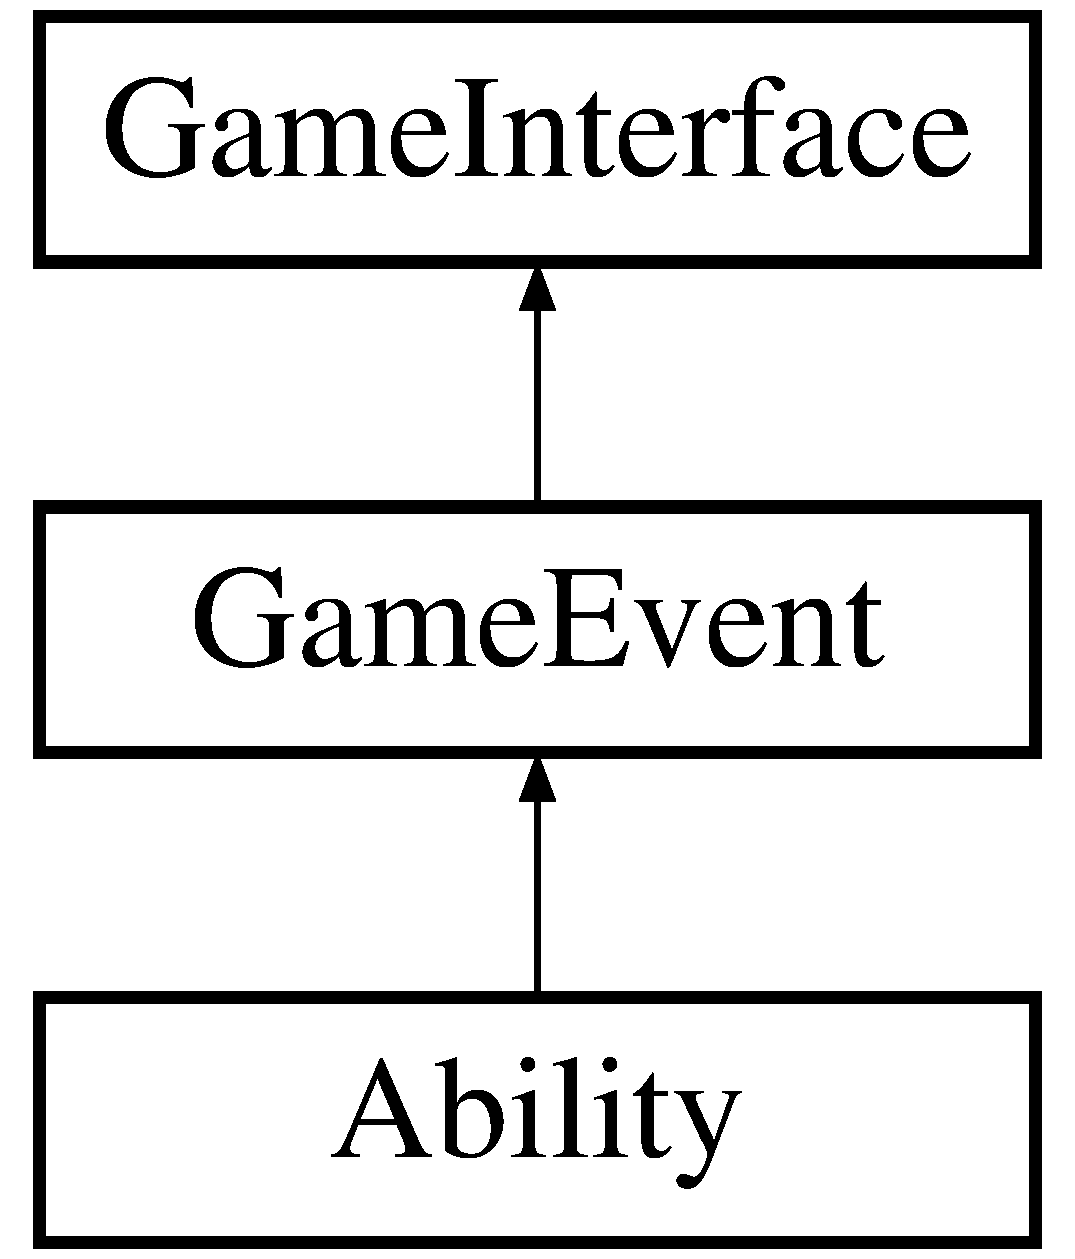
\includegraphics[height=3.000000cm]{class_game_event}
\end{center}
\end{figure}
\subsection*{Public Member Functions}
\begin{DoxyCompactItemize}
\item 
\hyperlink{class_game_event_a0a8133b65ffc98712879d18186ef3020}{Game\-Event} ()
\item 
\hyperlink{class_game_event_a7687b9408418c93c76af200475be6e2e}{Game\-Event} (const \hyperlink{class_game_event}{Game\-Event} \&other)
\item 
\hyperlink{class_game_event_a8a164c0919549846f667d7b0e9b80a72}{Game\-Event} (string symbol)
\item 
virtual \hyperlink{class_game_event_aaf514ed35c80bbbcc54ce411d9d71eef}{$\sim$\-Game\-Event} ()
\item 
\hyperlink{class_game_event}{Game\-Event} \& \hyperlink{class_game_event_a1b0fd750f2e764b1f47ac4c3fda27ebc}{operator=} (const \hyperlink{class_game_event}{Game\-Event} \&rhs)
\item 
virtual void \hyperlink{class_game_event_a0d21300957e0a82e4fcfdd7dd8ad9449}{operator()} ()
\item 
virtual void \hyperlink{class_game_event_a2effcb2226837b007cfb27defbd5658e}{notify} ()
\item 
string \hyperlink{class_game_event_a5013426766329f47e7eb0d2f88dbd8df}{draw} ()
\end{DoxyCompactItemize}
\subsection*{Protected Attributes}
\begin{DoxyCompactItemize}
\item 
unsigned \hyperlink{class_game_event_aecdf600e852c5a4f02f3cf2af0f6fe0f}{I\-D}
\item 
string \hyperlink{class_game_event_ab09ada74a9aeec15faeb99e2292534b2}{icon}
\end{DoxyCompactItemize}


\subsection{Detailed Description}


Definition at line 19 of file Game\-Event.\-h.



\subsection{Constructor \& Destructor Documentation}
\hypertarget{class_game_event_a0a8133b65ffc98712879d18186ef3020}{\index{Game\-Event@{Game\-Event}!Game\-Event@{Game\-Event}}
\index{Game\-Event@{Game\-Event}!GameEvent@{Game\-Event}}
\subsubsection[{Game\-Event}]{\setlength{\rightskip}{0pt plus 5cm}Game\-Event\-::\-Game\-Event (
\begin{DoxyParamCaption}
{}
\end{DoxyParamCaption}
)}}\label{class_game_event_a0a8133b65ffc98712879d18186ef3020}
Creates a new \hyperlink{class_game_event}{Game\-Event} 

Definition at line 14 of file Game\-Event.\-cpp.

\hypertarget{class_game_event_a7687b9408418c93c76af200475be6e2e}{\index{Game\-Event@{Game\-Event}!Game\-Event@{Game\-Event}}
\index{Game\-Event@{Game\-Event}!GameEvent@{Game\-Event}}
\subsubsection[{Game\-Event}]{\setlength{\rightskip}{0pt plus 5cm}Game\-Event\-::\-Game\-Event (
\begin{DoxyParamCaption}
\item[{const {\bf Game\-Event} \&}]{other}
\end{DoxyParamCaption}
)}}\label{class_game_event_a7687b9408418c93c76af200475be6e2e}
Copy constructor for \hyperlink{class_game_event}{Game\-Event}. The new instance has its own unique I\-D.


\begin{DoxyParams}{Parameters}
{\em other} & The \hyperlink{class_game_event}{Game\-Event} to be copied \\
\hline
\end{DoxyParams}


Definition at line 21 of file Game\-Event.\-cpp.

\hypertarget{class_game_event_a8a164c0919549846f667d7b0e9b80a72}{\index{Game\-Event@{Game\-Event}!Game\-Event@{Game\-Event}}
\index{Game\-Event@{Game\-Event}!GameEvent@{Game\-Event}}
\subsubsection[{Game\-Event}]{\setlength{\rightskip}{0pt plus 5cm}Game\-Event\-::\-Game\-Event (
\begin{DoxyParamCaption}
\item[{string}]{symbol}
\end{DoxyParamCaption}
)}}\label{class_game_event_a8a164c0919549846f667d7b0e9b80a72}
Creates an event with the given U\-T\-F-\/8 symbol (preferably just one character) as its icon


\begin{DoxyParams}{Parameters}
{\em symbol} & The icon to be used by this \hyperlink{class_game_event}{Game\-Event} \\
\hline
\end{DoxyParams}


Definition at line 28 of file Game\-Event.\-cpp.

\hypertarget{class_game_event_aaf514ed35c80bbbcc54ce411d9d71eef}{\index{Game\-Event@{Game\-Event}!$\sim$\-Game\-Event@{$\sim$\-Game\-Event}}
\index{$\sim$\-Game\-Event@{$\sim$\-Game\-Event}!GameEvent@{Game\-Event}}
\subsubsection[{$\sim$\-Game\-Event}]{\setlength{\rightskip}{0pt plus 5cm}Game\-Event\-::$\sim$\-Game\-Event (
\begin{DoxyParamCaption}
{}
\end{DoxyParamCaption}
)\hspace{0.3cm}{\ttfamily [virtual]}}}\label{class_game_event_aaf514ed35c80bbbcc54ce411d9d71eef}
Destructor for \hyperlink{class_game_event}{Game\-Event} 

Definition at line 35 of file Game\-Event.\-cpp.



\subsection{Member Function Documentation}
\hypertarget{class_game_event_a5013426766329f47e7eb0d2f88dbd8df}{\index{Game\-Event@{Game\-Event}!draw@{draw}}
\index{draw@{draw}!GameEvent@{Game\-Event}}
\subsubsection[{draw}]{\setlength{\rightskip}{0pt plus 5cm}string Game\-Event\-::draw (
\begin{DoxyParamCaption}
{}
\end{DoxyParamCaption}
)}}\label{class_game_event_a5013426766329f47e7eb0d2f88dbd8df}


Definition at line 57 of file Game\-Event.\-cpp.

\hypertarget{class_game_event_a2effcb2226837b007cfb27defbd5658e}{\index{Game\-Event@{Game\-Event}!notify@{notify}}
\index{notify@{notify}!GameEvent@{Game\-Event}}
\subsubsection[{notify}]{\setlength{\rightskip}{0pt plus 5cm}void Game\-Event\-::notify (
\begin{DoxyParamCaption}
{}
\end{DoxyParamCaption}
)\hspace{0.3cm}{\ttfamily [virtual]}}}\label{class_game_event_a2effcb2226837b007cfb27defbd5658e}


Reimplemented in \hyperlink{class_ability_a1a960040b98f8632a675ad184ead84b3}{Ability}.



Definition at line 53 of file Game\-Event.\-cpp.

\hypertarget{class_game_event_a0d21300957e0a82e4fcfdd7dd8ad9449}{\index{Game\-Event@{Game\-Event}!operator()@{operator()}}
\index{operator()@{operator()}!GameEvent@{Game\-Event}}
\subsubsection[{operator()}]{\setlength{\rightskip}{0pt plus 5cm}void Game\-Event\-::operator() (
\begin{DoxyParamCaption}
{}
\end{DoxyParamCaption}
)\hspace{0.3cm}{\ttfamily [virtual]}}}\label{class_game_event_a0d21300957e0a82e4fcfdd7dd8ad9449}
An implementing class can define a default function by overloading its () operator 

Implements \hyperlink{class_game_interface_aa47ddf1a598f94dc6273e5d06834f435}{Game\-Interface}.



Reimplemented in \hyperlink{class_ability_af5d8c9005cc4b4b2a8f650cc10529924}{Ability}.



Definition at line 49 of file Game\-Event.\-cpp.

\hypertarget{class_game_event_a1b0fd750f2e764b1f47ac4c3fda27ebc}{\index{Game\-Event@{Game\-Event}!operator=@{operator=}}
\index{operator=@{operator=}!GameEvent@{Game\-Event}}
\subsubsection[{operator=}]{\setlength{\rightskip}{0pt plus 5cm}{\bf Game\-Event} \& Game\-Event\-::operator= (
\begin{DoxyParamCaption}
\item[{const {\bf Game\-Event} \&}]{rhs}
\end{DoxyParamCaption}
)}}\label{class_game_event_a1b0fd750f2e764b1f47ac4c3fda27ebc}
Assignment operator overload for \hyperlink{class_game_event}{Game\-Event}. The object copied to will have its own unique I\-D.


\begin{DoxyParams}{Parameters}
{\em rhs} & The right hand side argument (which will be copied) \\
\hline
\end{DoxyParams}


Definition at line 40 of file Game\-Event.\-cpp.



\subsection{Member Data Documentation}
\hypertarget{class_game_event_ab09ada74a9aeec15faeb99e2292534b2}{\index{Game\-Event@{Game\-Event}!icon@{icon}}
\index{icon@{icon}!GameEvent@{Game\-Event}}
\subsubsection[{icon}]{\setlength{\rightskip}{0pt plus 5cm}string Game\-Event\-::icon\hspace{0.3cm}{\ttfamily [protected]}}}\label{class_game_event_ab09ada74a9aeec15faeb99e2292534b2}


Definition at line 28 of file Game\-Event.\-h.

\hypertarget{class_game_event_aecdf600e852c5a4f02f3cf2af0f6fe0f}{\index{Game\-Event@{Game\-Event}!I\-D@{I\-D}}
\index{I\-D@{I\-D}!GameEvent@{Game\-Event}}
\subsubsection[{I\-D}]{\setlength{\rightskip}{0pt plus 5cm}unsigned Game\-Event\-::\-I\-D\hspace{0.3cm}{\ttfamily [protected]}}}\label{class_game_event_aecdf600e852c5a4f02f3cf2af0f6fe0f}


Definition at line 27 of file Game\-Event.\-h.



The documentation for this class was generated from the following files\-:\begin{DoxyCompactItemize}
\item 
/\-Volumes/\-O\-S X H\-D\-D/\-Users/\-Adam/\-Developer/\-Sprite\-Fight/\-World/\hyperlink{_game_event_8h}{Game\-Event.\-h}\item 
/\-Volumes/\-O\-S X H\-D\-D/\-Users/\-Adam/\-Developer/\-Sprite\-Fight/\-World/\hyperlink{_game_event_8cpp}{Game\-Event.\-cpp}\end{DoxyCompactItemize}

\hypertarget{class_game_interface}{\section{Game\-Interface Class Reference}
\label{class_game_interface}\index{Game\-Interface@{Game\-Interface}}
}


{\ttfamily \#include $<$Game\-Interface.\-h$>$}

Inheritance diagram for Game\-Interface\-:\begin{figure}[H]
\begin{center}
\leavevmode
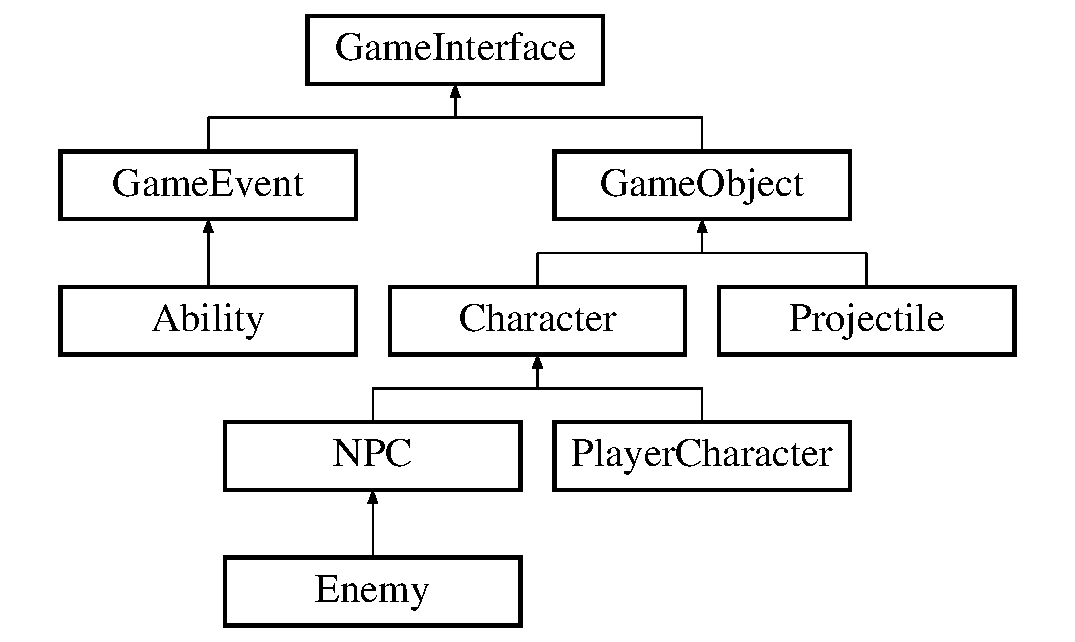
\includegraphics[height=5.000000cm]{class_game_interface}
\end{center}
\end{figure}
\subsection*{Public Member Functions}
\begin{DoxyCompactItemize}
\item 
virtual void \hyperlink{class_game_interface_aa47ddf1a598f94dc6273e5d06834f435}{operator()} ()=0
\item 
virtual void \hyperlink{class_game_interface_aac4337d6b69549d389ff7d1b167fd7be}{update} ()=0
\item 
virtual void \hyperlink{class_game_interface_ac451407fef525c7114bbd3a2e3d17799}{move\-Up} ()=0
\item 
virtual void \hyperlink{class_game_interface_a6899c1e5b3f48ed7892791e540a4c55c}{move\-Down} ()=0
\item 
virtual void \hyperlink{class_game_interface_a4eb03058ca25e4b741f4203e5a2f44b8}{move\-Right} ()=0
\item 
virtual void \hyperlink{class_game_interface_a66cbd9c9e07a5abca69879431346e1ea}{move\-Left} ()=0
\item 
virtual void \hyperlink{class_game_interface_a7dc8aef4e9339745250c77e8b41ee1b2}{jump} ()=0
\item 
virtual void \hyperlink{class_game_interface_af3f525cdb14ebc3c6b139780c1d5f318}{fire} ()=0
\end{DoxyCompactItemize}


\subsection{Detailed Description}
The pure virtual base class that will serve as an interface to every object in the game world. It defines all methods by which any class can talk to another. Since \hyperlink{class_key_input_register}{Key\-Input\-Register} expects an instance of \hyperlink{class_game_interface}{Game\-Interface} for member function calls, of Any class that wishes to make its its methods available for callback from input events should add a pure virtual version of said functions to \hyperlink{class_game_interface}{Game\-Interface}, inherit from \hyperlink{class_game_interface}{Game\-Interface}, and implement. 

Definition at line 26 of file Game\-Interface.\-h.



\subsection{Member Function Documentation}
\hypertarget{class_game_interface_af3f525cdb14ebc3c6b139780c1d5f318}{\index{Game\-Interface@{Game\-Interface}!fire@{fire}}
\index{fire@{fire}!GameInterface@{Game\-Interface}}
\subsubsection[{fire}]{\setlength{\rightskip}{0pt plus 5cm}virtual void Game\-Interface\-::fire (
\begin{DoxyParamCaption}
{}
\end{DoxyParamCaption}
)\hspace{0.3cm}{\ttfamily [pure virtual]}}}\label{class_game_interface_af3f525cdb14ebc3c6b139780c1d5f318}


Implemented in \hyperlink{class_game_object_aefab5eddd7dfc186c7e5ba34bbefce41}{Game\-Object}, and \hyperlink{class_player_character_a646ce764c65c544fe4b76912b3fd15e5}{Player\-Character}.

\hypertarget{class_game_interface_a7dc8aef4e9339745250c77e8b41ee1b2}{\index{Game\-Interface@{Game\-Interface}!jump@{jump}}
\index{jump@{jump}!GameInterface@{Game\-Interface}}
\subsubsection[{jump}]{\setlength{\rightskip}{0pt plus 5cm}virtual void Game\-Interface\-::jump (
\begin{DoxyParamCaption}
{}
\end{DoxyParamCaption}
)\hspace{0.3cm}{\ttfamily [pure virtual]}}}\label{class_game_interface_a7dc8aef4e9339745250c77e8b41ee1b2}


Implemented in \hyperlink{class_game_object_aa8b87ef4a487c54c1d5b327c001b5c84}{Game\-Object}, and \hyperlink{class_player_character_ab67b7f795e75b73027620483bea2871b}{Player\-Character}.

\hypertarget{class_game_interface_a6899c1e5b3f48ed7892791e540a4c55c}{\index{Game\-Interface@{Game\-Interface}!move\-Down@{move\-Down}}
\index{move\-Down@{move\-Down}!GameInterface@{Game\-Interface}}
\subsubsection[{move\-Down}]{\setlength{\rightskip}{0pt plus 5cm}virtual void Game\-Interface\-::move\-Down (
\begin{DoxyParamCaption}
{}
\end{DoxyParamCaption}
)\hspace{0.3cm}{\ttfamily [pure virtual]}}}\label{class_game_interface_a6899c1e5b3f48ed7892791e540a4c55c}


Implemented in \hyperlink{class_game_object_ab2d6fdbc50ff110d3a6d101e3539dca9}{Game\-Object}.

\hypertarget{class_game_interface_a66cbd9c9e07a5abca69879431346e1ea}{\index{Game\-Interface@{Game\-Interface}!move\-Left@{move\-Left}}
\index{move\-Left@{move\-Left}!GameInterface@{Game\-Interface}}
\subsubsection[{move\-Left}]{\setlength{\rightskip}{0pt plus 5cm}virtual void Game\-Interface\-::move\-Left (
\begin{DoxyParamCaption}
{}
\end{DoxyParamCaption}
)\hspace{0.3cm}{\ttfamily [pure virtual]}}}\label{class_game_interface_a66cbd9c9e07a5abca69879431346e1ea}


Implemented in \hyperlink{class_game_object_a71152debfe014bef0efe7464dd45aacb}{Game\-Object}.

\hypertarget{class_game_interface_a4eb03058ca25e4b741f4203e5a2f44b8}{\index{Game\-Interface@{Game\-Interface}!move\-Right@{move\-Right}}
\index{move\-Right@{move\-Right}!GameInterface@{Game\-Interface}}
\subsubsection[{move\-Right}]{\setlength{\rightskip}{0pt plus 5cm}virtual void Game\-Interface\-::move\-Right (
\begin{DoxyParamCaption}
{}
\end{DoxyParamCaption}
)\hspace{0.3cm}{\ttfamily [pure virtual]}}}\label{class_game_interface_a4eb03058ca25e4b741f4203e5a2f44b8}


Implemented in \hyperlink{class_game_object_abb75fa4bde389384815abb7cacc35045}{Game\-Object}.

\hypertarget{class_game_interface_ac451407fef525c7114bbd3a2e3d17799}{\index{Game\-Interface@{Game\-Interface}!move\-Up@{move\-Up}}
\index{move\-Up@{move\-Up}!GameInterface@{Game\-Interface}}
\subsubsection[{move\-Up}]{\setlength{\rightskip}{0pt plus 5cm}virtual void Game\-Interface\-::move\-Up (
\begin{DoxyParamCaption}
{}
\end{DoxyParamCaption}
)\hspace{0.3cm}{\ttfamily [pure virtual]}}}\label{class_game_interface_ac451407fef525c7114bbd3a2e3d17799}


Implemented in \hyperlink{class_game_object_a2c4862885319288c746d8e1c454556b6}{Game\-Object}.

\hypertarget{class_game_interface_aa47ddf1a598f94dc6273e5d06834f435}{\index{Game\-Interface@{Game\-Interface}!operator()@{operator()}}
\index{operator()@{operator()}!GameInterface@{Game\-Interface}}
\subsubsection[{operator()}]{\setlength{\rightskip}{0pt plus 5cm}virtual void Game\-Interface\-::operator() (
\begin{DoxyParamCaption}
{}
\end{DoxyParamCaption}
)\hspace{0.3cm}{\ttfamily [pure virtual]}}}\label{class_game_interface_aa47ddf1a598f94dc6273e5d06834f435}
An implementing class can define a default function by overloading its () operator 

Implemented in \hyperlink{class_game_object_ab8fccd5edcbebad0553aa4336a71452a}{Game\-Object}, \hyperlink{class_character_a3c4dfc59865fe39251070cd0b92d34ac}{Character}, \hyperlink{class_player_character_a067c5b11f7deafd448726ec4ac294b03}{Player\-Character}, \hyperlink{class_n_p_c_a73befe685fef40ab7f1ac954d932697d}{N\-P\-C}, \hyperlink{class_game_event_a0d21300957e0a82e4fcfdd7dd8ad9449}{Game\-Event}, and \hyperlink{class_ability_af5d8c9005cc4b4b2a8f650cc10529924}{Ability}.

\hypertarget{class_game_interface_aac4337d6b69549d389ff7d1b167fd7be}{\index{Game\-Interface@{Game\-Interface}!update@{update}}
\index{update@{update}!GameInterface@{Game\-Interface}}
\subsubsection[{update}]{\setlength{\rightskip}{0pt plus 5cm}virtual void Game\-Interface\-::update (
\begin{DoxyParamCaption}
{}
\end{DoxyParamCaption}
)\hspace{0.3cm}{\ttfamily [pure virtual]}}}\label{class_game_interface_aac4337d6b69549d389ff7d1b167fd7be}


Implemented in \hyperlink{class_player_character_a2ac275d3de97c5ecc260e93e0585168a}{Player\-Character}, and \hyperlink{class_game_object_adad7d284b670db722a2fda8e6a7997e3}{Game\-Object}.



The documentation for this class was generated from the following file\-:\begin{DoxyCompactItemize}
\item 
/\-Volumes/\-O\-S X H\-D\-D/\-Users/\-Adam/\-Developer/\-Sprite\-Fight/\-World/\hyperlink{_game_interface_8h}{Game\-Interface.\-h}\end{DoxyCompactItemize}

\hypertarget{class_game_map}{\section{Game\-Map$<$ T $>$ Class Template Reference}
\label{class_game_map}\index{Game\-Map$<$ T $>$@{Game\-Map$<$ T $>$}}
}


{\ttfamily \#include $<$Forward\-Decl.\-h$>$}

\subsection*{Public Member Functions}
\begin{DoxyCompactItemize}
\item 
{\footnotesize template$<$typename N $>$ }\\\hyperlink{class_game_map_aaf385841d0390f0b2b21fd6e2553c72e}{Game\-Map} (N max\-X, N max\-Y)
\item 
\hyperlink{class_game_map_a4bfac2bbaabb053fad5616666e222691}{$\sim$\-Game\-Map} ()
\item 
vector$<$ vector$<$ deque$<$ T $\ast$ $>$ $>$ $\ast$ $>$ $\ast$ \hyperlink{class_game_map_a47d97dc86ca0b91866b48dcaa9fa39a2}{get\-Map\-Vect} ()
\item 
unsigned long \hyperlink{class_game_map_abce7a6939365afdcab7bb29399a68ac1}{get\-X\-Bound} ()
\item 
unsigned long \hyperlink{class_game_map_a14de3740816e5328fcc2580363e51f18}{get\-Y\-Bound} ()
\item 
{\footnotesize template$<$typename N $>$ }\\void \hyperlink{class_game_map_aa38c0f97584d3b5b1b78389c94ad194f}{place} (\hyperlink{struct_position}{Position}$<$ N $>$ $\ast$where, T $\ast$pointer\-To\-Original\-Object, const \hyperlink{struct_bounds_check}{Bounds\-Check}$<$ N $>$ check)
\item 
{\footnotesize template$<$typename N $>$ }\\void \hyperlink{class_game_map_ad171ac0784575bfe68c9ad224fcf05ad}{erase} (const \hyperlink{struct_position}{Position}$<$ N $>$ $\ast$\hyperlink{class_game_map_ad9b90d1652b7db7d72370d10b361278d}{current\-Loc}, T $\ast$pointer\-To\-Original\-Object)
\item 
{\footnotesize template$<$typename N $>$ }\\void \hyperlink{class_game_map_a8aca03fd075ee28bbf65b917eb9a3449}{map\-\_\-move} (const \hyperlink{struct_position}{Position}$<$ N $>$ \&\hyperlink{class_game_map_ad9b90d1652b7db7d72370d10b361278d}{current\-Loc}, const \hyperlink{struct_position}{Position}$<$ N $>$ \&to\-New\-Loc, T $\ast$pointer\-To\-Original\-Object)
\item 
{\footnotesize template$<$typename N $>$ }\\list$<$ T $\ast$ $>$ $\ast$ \hyperlink{class_game_map_afc7638e97c9fedbac81f5b88243e9c0a}{at\-\_\-pos} (const \hyperlink{struct_position}{Position}$<$ N $>$ $\ast$where)
\item 
{\footnotesize template$<$typename N $>$ }\\\hyperlink{struct_position}{Position}$<$ N $>$ \hyperlink{class_game_map_ad9b90d1652b7db7d72370d10b361278d}{current\-Loc} (T $\ast$obj)
\item 
{\footnotesize template$<$typename N $>$ }\\vector$<$ T $\ast$ $>$ $\ast$ \hyperlink{class_game_map_a2a632a97e225ec9fe54a13fc05ae45fa}{find\-Nearby} (const \hyperlink{struct_position}{Position}$<$ N $>$ $\ast$start, const N x\-\_\-lim, const N y\-\_\-lim)
\end{DoxyCompactItemize}
\subsection*{Public Attributes}
\begin{DoxyCompactItemize}
\item 
bool \hyperlink{class_game_map_a2958e7779794322ace38425b689b38f6}{search\-Success} = false
\end{DoxyCompactItemize}


\subsection{Detailed Description}
\subsubsection*{template$<$class T$>$class Game\-Map$<$ T $>$}



Definition at line 18 of file Forward\-Decl.\-h.



\subsection{Constructor \& Destructor Documentation}
\hypertarget{class_game_map_aaf385841d0390f0b2b21fd6e2553c72e}{\index{Game\-Map@{Game\-Map}!Game\-Map@{Game\-Map}}
\index{Game\-Map@{Game\-Map}!GameMap@{Game\-Map}}
\subsubsection[{Game\-Map}]{\setlength{\rightskip}{0pt plus 5cm}template$<$class T $>$ template$<$typename N $>$ {\bf Game\-Map}$<$ T $>$\-::{\bf Game\-Map} (
\begin{DoxyParamCaption}
\item[{N}]{max\-X, }
\item[{N}]{max\-Y}
\end{DoxyParamCaption}
)}}\label{class_game_map_aaf385841d0390f0b2b21fd6e2553c72e}


Definition at line 99 of file Game\-Map.\-hpp.

\hypertarget{class_game_map_a4bfac2bbaabb053fad5616666e222691}{\index{Game\-Map@{Game\-Map}!$\sim$\-Game\-Map@{$\sim$\-Game\-Map}}
\index{$\sim$\-Game\-Map@{$\sim$\-Game\-Map}!GameMap@{Game\-Map}}
\subsubsection[{$\sim$\-Game\-Map}]{\setlength{\rightskip}{0pt plus 5cm}template$<$class T $>$ {\bf Game\-Map}$<$ T $>$\-::$\sim${\bf Game\-Map} (
\begin{DoxyParamCaption}
{}
\end{DoxyParamCaption}
)}}\label{class_game_map_a4bfac2bbaabb053fad5616666e222691}


Definition at line 112 of file Game\-Map.\-hpp.



\subsection{Member Function Documentation}
\hypertarget{class_game_map_afc7638e97c9fedbac81f5b88243e9c0a}{\index{Game\-Map@{Game\-Map}!at\-\_\-pos@{at\-\_\-pos}}
\index{at\-\_\-pos@{at\-\_\-pos}!GameMap@{Game\-Map}}
\subsubsection[{at\-\_\-pos}]{\setlength{\rightskip}{0pt plus 5cm}template$<$class T $>$ template$<$typename N $>$ list$<$ T $\ast$ $>$ $\ast$ {\bf Game\-Map}$<$ T $>$\-::at\-\_\-pos (
\begin{DoxyParamCaption}
\item[{const {\bf Position}$<$ N $>$ $\ast$}]{where}
\end{DoxyParamCaption}
)}}\label{class_game_map_afc7638e97c9fedbac81f5b88243e9c0a}
Returns the first object at this Position$<$\-N$>$ 

Definition at line 211 of file Game\-Map.\-hpp.

\hypertarget{class_game_map_ad9b90d1652b7db7d72370d10b361278d}{\index{Game\-Map@{Game\-Map}!current\-Loc@{current\-Loc}}
\index{current\-Loc@{current\-Loc}!GameMap@{Game\-Map}}
\subsubsection[{current\-Loc}]{\setlength{\rightskip}{0pt plus 5cm}template$<$class T$>$ template$<$typename N $>$ {\bf Position}$<$ N $>$ {\bf Game\-Map}$<$ T $>$\-::current\-Loc (
\begin{DoxyParamCaption}
\item[{T $\ast$}]{obj}
\end{DoxyParamCaption}
)}}\label{class_game_map_ad9b90d1652b7db7d72370d10b361278d}


Definition at line 219 of file Game\-Map.\-hpp.

\hypertarget{class_game_map_ad171ac0784575bfe68c9ad224fcf05ad}{\index{Game\-Map@{Game\-Map}!erase@{erase}}
\index{erase@{erase}!GameMap@{Game\-Map}}
\subsubsection[{erase}]{\setlength{\rightskip}{0pt plus 5cm}template$<$class T$>$ template$<$typename N $>$ void {\bf Game\-Map}$<$ T $>$\-::erase (
\begin{DoxyParamCaption}
\item[{const {\bf Position}$<$ N $>$ $\ast$}]{current\-Loc, }
\item[{T $\ast$}]{pointer\-To\-Original\-Object}
\end{DoxyParamCaption}
)}}\label{class_game_map_ad171ac0784575bfe68c9ad224fcf05ad}


Definition at line 241 of file Game\-Map.\-hpp.

\hypertarget{class_game_map_a2a632a97e225ec9fe54a13fc05ae45fa}{\index{Game\-Map@{Game\-Map}!find\-Nearby@{find\-Nearby}}
\index{find\-Nearby@{find\-Nearby}!GameMap@{Game\-Map}}
\subsubsection[{find\-Nearby}]{\setlength{\rightskip}{0pt plus 5cm}template$<$class T $>$ template$<$typename N $>$ vector$<$ T $\ast$ $>$ $\ast$ {\bf Game\-Map}$<$ T $>$\-::find\-Nearby (
\begin{DoxyParamCaption}
\item[{const {\bf Position}$<$ N $>$ $\ast$}]{start, }
\item[{const N}]{x\-\_\-lim, }
\item[{const N}]{y\-\_\-lim}
\end{DoxyParamCaption}
)}}\label{class_game_map_a2a632a97e225ec9fe54a13fc05ae45fa}
Searches within the specified limits for an object of the specified type. Returns a nullptr if none found


\begin{DoxyParams}{Parameters}
{\em start} & The Position$<$\-N$>$ of the object that wants to search for nearby objects \\
\hline
{\em x\-\_\-lim} & The maximum distance to search longtitudinally \\
\hline
{\em y\-\_\-lim} & The maximum distance to search latitudinally \\
\hline
\end{DoxyParams}


Definition at line 282 of file Game\-Map.\-hpp.

\hypertarget{class_game_map_a47d97dc86ca0b91866b48dcaa9fa39a2}{\index{Game\-Map@{Game\-Map}!get\-Map\-Vect@{get\-Map\-Vect}}
\index{get\-Map\-Vect@{get\-Map\-Vect}!GameMap@{Game\-Map}}
\subsubsection[{get\-Map\-Vect}]{\setlength{\rightskip}{0pt plus 5cm}template$<$class T$>$ vector$<$ vector$<$ deque$<$T $\ast$$>$ $>$ $\ast$$>$$\ast$ {\bf Game\-Map}$<$ T $>$\-::get\-Map\-Vect (
\begin{DoxyParamCaption}
{}
\end{DoxyParamCaption}
)\hspace{0.3cm}{\ttfamily [inline]}}}\label{class_game_map_a47d97dc86ca0b91866b48dcaa9fa39a2}


Definition at line 53 of file Game\-Map.\-hpp.

\hypertarget{class_game_map_abce7a6939365afdcab7bb29399a68ac1}{\index{Game\-Map@{Game\-Map}!get\-X\-Bound@{get\-X\-Bound}}
\index{get\-X\-Bound@{get\-X\-Bound}!GameMap@{Game\-Map}}
\subsubsection[{get\-X\-Bound}]{\setlength{\rightskip}{0pt plus 5cm}template$<$class T$>$ unsigned long {\bf Game\-Map}$<$ T $>$\-::get\-X\-Bound (
\begin{DoxyParamCaption}
{}
\end{DoxyParamCaption}
)\hspace{0.3cm}{\ttfamily [inline]}}}\label{class_game_map_abce7a6939365afdcab7bb29399a68ac1}


Definition at line 55 of file Game\-Map.\-hpp.

\hypertarget{class_game_map_a14de3740816e5328fcc2580363e51f18}{\index{Game\-Map@{Game\-Map}!get\-Y\-Bound@{get\-Y\-Bound}}
\index{get\-Y\-Bound@{get\-Y\-Bound}!GameMap@{Game\-Map}}
\subsubsection[{get\-Y\-Bound}]{\setlength{\rightskip}{0pt plus 5cm}template$<$class T$>$ unsigned long {\bf Game\-Map}$<$ T $>$\-::get\-Y\-Bound (
\begin{DoxyParamCaption}
{}
\end{DoxyParamCaption}
)\hspace{0.3cm}{\ttfamily [inline]}}}\label{class_game_map_a14de3740816e5328fcc2580363e51f18}


Definition at line 56 of file Game\-Map.\-hpp.

\hypertarget{class_game_map_a8aca03fd075ee28bbf65b917eb9a3449}{\index{Game\-Map@{Game\-Map}!map\-\_\-move@{map\-\_\-move}}
\index{map\-\_\-move@{map\-\_\-move}!GameMap@{Game\-Map}}
\subsubsection[{map\-\_\-move}]{\setlength{\rightskip}{0pt plus 5cm}template$<$class T$>$ template$<$typename N $>$ void {\bf Game\-Map}$<$ T $>$\-::map\-\_\-move (
\begin{DoxyParamCaption}
\item[{const {\bf Position}$<$ N $>$ \&}]{current\-Loc, }
\item[{const {\bf Position}$<$ N $>$ \&}]{to\-New\-Loc, }
\item[{T $\ast$}]{pointer\-To\-Original\-Object}
\end{DoxyParamCaption}
)}}\label{class_game_map_a8aca03fd075ee28bbf65b917eb9a3449}
Moves the object to a new Position$<$\-N$>$ on the map, and erases (calls \hyperlink{class_game_map_ad171ac0784575bfe68c9ad224fcf05ad}{erase()}) on its old Position$<$\-N$>$ 

Definition at line 203 of file Game\-Map.\-hpp.

\hypertarget{class_game_map_aa38c0f97584d3b5b1b78389c94ad194f}{\index{Game\-Map@{Game\-Map}!place@{place}}
\index{place@{place}!GameMap@{Game\-Map}}
\subsubsection[{place}]{\setlength{\rightskip}{0pt plus 5cm}template$<$class T$>$ template$<$typename N $>$ void {\bf Game\-Map}$<$ T $>$\-::place (
\begin{DoxyParamCaption}
\item[{{\bf Position}$<$ N $>$ $\ast$}]{where, }
\item[{T $\ast$}]{pointer\-To\-Original\-Object, }
\item[{const {\bf Bounds\-Check}$<$ N $>$}]{check}
\end{DoxyParamCaption}
)}}\label{class_game_map_aa38c0f97584d3b5b1b78389c94ad194f}
Places pointer\-To\-Original\-Object at \hyperlink{struct_position}{Position} where. 

Definition at line 135 of file Game\-Map.\-hpp.



\subsection{Member Data Documentation}
\hypertarget{class_game_map_a2958e7779794322ace38425b689b38f6}{\index{Game\-Map@{Game\-Map}!search\-Success@{search\-Success}}
\index{search\-Success@{search\-Success}!GameMap@{Game\-Map}}
\subsubsection[{search\-Success}]{\setlength{\rightskip}{0pt plus 5cm}template$<$class T$>$ bool {\bf Game\-Map}$<$ T $>$\-::search\-Success = false}}\label{class_game_map_a2958e7779794322ace38425b689b38f6}


Definition at line 42 of file Game\-Map.\-hpp.



The documentation for this class was generated from the following files\-:\begin{DoxyCompactItemize}
\item 
/\-Volumes/\-O\-S X H\-D\-D/\-Users/\-Adam/\-Developer/\-Sprite\-Fight/\-World/\hyperlink{_forward_decl_8h}{Forward\-Decl.\-h}\item 
/\-Volumes/\-O\-S X H\-D\-D/\-Users/\-Adam/\-Developer/\-Sprite\-Fight/\-World/\hyperlink{_game_map_8hpp}{Game\-Map.\-hpp}\end{DoxyCompactItemize}

\hypertarget{class_game_object}{\section{Game\-Object Class Reference}
\label{class_game_object}\index{Game\-Object@{Game\-Object}}
}


The base class from which all other classes in the world will inherit. This class will handle the assignment of a unique I\-D to each \hyperlink{class_game_object}{Game\-Object}.  




{\ttfamily \#include $<$Game\-Object.\-h$>$}

Inheritance diagram for Game\-Object\-:\begin{figure}[H]
\begin{center}
\leavevmode
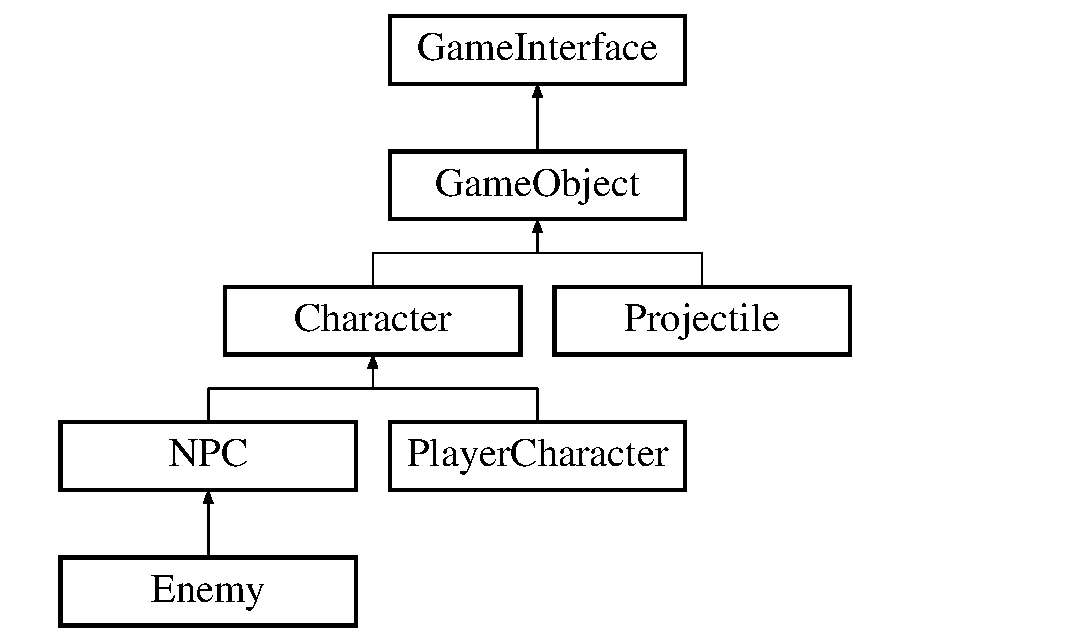
\includegraphics[height=5.000000cm]{class_game_object}
\end{center}
\end{figure}
\subsection*{Public Member Functions}
\begin{DoxyCompactItemize}
\item 
\hyperlink{class_game_object_a0348e3ee2e83d56eafca7a3547f432c4}{Game\-Object} ()
\item 
\hyperlink{class_game_object_ab13374d070cfe6a1459539d54c671eba}{Game\-Object} (const \hyperlink{class_game_object}{Game\-Object} \&other)
\item 
\hyperlink{class_game_object_ab415bbda3ab836e5de5e73c0a9d50ba3}{Game\-Object} (\hyperlink{class_game_object}{Game\-Object} \&\&other)
\item 
\hyperlink{class_game_object_af784d96f9ca701cd705050ce1baf6bd2}{Game\-Object} (const \hyperlink{struct_asset_file}{Asset\-File} \&image\-File, float size\-Modifier, const \hyperlink{struct_position}{Position}$<$ float $>$ \&\hyperlink{class_game_object_a6858e668e7d2c5ded850b952aaacd905}{loc}, bool visible, bool monitor\-Velocity)
\item 
\hyperlink{class_game_object_a039a66e3278f6a75ad0021ffda1b1a71}{Game\-Object} (\hyperlink{class_fast_rand}{Fast\-Rand}$<$ int $>$ rand)
\item 
virtual \hyperlink{class_game_object_ab82dfdb656f9051c0587e6593b2dda97}{$\sim$\-Game\-Object} ()
\item 
virtual \hyperlink{class_game_object}{Game\-Object} \& \hyperlink{class_game_object_afa8505b16b7f5fe0b825d59fcee17291}{operator=} (const \hyperlink{class_game_object}{Game\-Object} \&rhs)
\item 
virtual \hyperlink{class_game_object}{Game\-Object} \& \hyperlink{class_game_object_a428579a3f2d8eb2c9e37bd4452d18d3b}{operator=} (\hyperlink{class_game_object}{Game\-Object} \&\&rhs)
\item 
virtual void \hyperlink{class_game_object_ab8fccd5edcbebad0553aa4336a71452a}{operator()} ()
\item 
virtual void \hyperlink{class_game_object_afe9e6ee87d3062c80a9c560a12bfc279}{operator()} (\hyperlink{class_game_object}{Game\-Object} $\ast$other)
\item 
bool \hyperlink{class_game_object_ab8e7bb6eaae69c9e282efb22c3996499}{operator==} (\hyperlink{class_game_object}{Game\-Object} \&other) const 
\item 
unsigned \hyperlink{class_game_object_ac4692b8584d58cabc918e53e54767008}{get\-I\-D} ()
\item 
virtual void \hyperlink{class_game_object_a9867e75f8cfc4df52d03467aca07a4ac}{notify} ()
\item 
virtual void \hyperlink{class_game_object_ad7f752f1e3c84bd74de6110c17df3938}{pass\-Message} (\hyperlink{struct_message}{Message} $\ast$message, \hyperlink{class_game_object}{Game\-Object} \&recipient)
\item 
virtual void \hyperlink{class_game_object_adc249c683994a9c74b518a82fc22dbab}{text\-Description} (ostream $\ast$write\-To) const 
\item 
void \hyperlink{class_game_object_ae483f641380cd7d30c8bc469ffa2b219}{move\-To} (\hyperlink{struct_position}{Position}$<$ float $>$ $\ast$to)
\item 
void \hyperlink{class_game_object_ac9da7fd4807118db721e2d1cbee69580}{move\-To} (\hyperlink{struct_position}{Position}$<$ float $>$ to)
\item 
void \hyperlink{class_game_object_a34a64493de5a087b7cb79e1fceb5db8e}{move\-To} (float x, float y, float z)
\item 
void \hyperlink{class_game_object_af0f7a85d5565aa73554140b7cb876af0}{move\-X} (float x)
\item 
void \hyperlink{class_game_object_ab7e675ee37da1f4dfe9ce59de2df3a25}{move\-Y} (float y)
\item 
virtual void \hyperlink{class_game_object_a2c4862885319288c746d8e1c454556b6}{move\-Up} ()
\item 
virtual void \hyperlink{class_game_object_ab2d6fdbc50ff110d3a6d101e3539dca9}{move\-Down} ()
\item 
virtual void \hyperlink{class_game_object_abb75fa4bde389384815abb7cacc35045}{move\-Right} ()
\item 
virtual void \hyperlink{class_game_object_a71152debfe014bef0efe7464dd45aacb}{move\-Left} ()
\item 
virtual void \hyperlink{class_game_object_ac279191d7c42ca8ad3e1dd2baf5a9519}{move\-Random\-Direction} ()
\item 
void \hyperlink{class_game_object_aa8b87ef4a487c54c1d5b327c001b5c84}{jump} ()
\item 
void \hyperlink{class_game_object_aebf4e54c90de73d56186beaebead1ccc}{move} (float distance\-Modifier=\hyperlink{_default_config_8h_ae612ff4d109725baa6322f37db537175}{default\-Move\-Distance}$<$ float $>$)
\item 
virtual void \hyperlink{class_game_object_a41d5ef30ab6863ac5277fbc37297b11b}{move\-New\-Direction} (const \hyperlink{struct_vectr}{Vectr}$<$ float $>$ \&new\-Direction)
\item 
void \hyperlink{class_game_object_a372fee85f1892fd1fe258061dfb13269}{wander} ()
\item 
virtual void \hyperlink{class_game_object_a565a3950ea0af84bf7515bdb77abf51a}{default\-Behaviors} ()
\item 
virtual void \hyperlink{class_game_object_a43862b5d602a0fec32b686ab8586e886}{ai\-Behaviors} ()
\item 
virtual void \hyperlink{class_game_object_a87cfdf508b01dd9653716a5b4f4d7571}{attack} (\hyperlink{class_game_object}{Game\-Object} $\ast$enemy)
\item 
virtual void \hyperlink{class_game_object_a6bfde6f1f94ce0bf66f598dc53a75551}{find\-Nearby\-Ally} (int search\-Distance\-X, int search\-Distance\-Y)
\item 
virtual void \hyperlink{class_game_object_a20ca237d244a3eeb34500e0134d60eb1}{ally\-With} (const \hyperlink{class_game_object}{Game\-Object} $\ast$)
\item 
\hyperlink{_character_data_8h_a55ecd4f2ec2ebfe8d5b0163e4ac2a967}{Colors} \hyperlink{class_game_object_afa75c94bc4f7f52a48d000ef0803ec59}{get\-Color} () const 
\item 
const \hyperlink{struct_position}{Position}$<$ float $>$ $\ast$ \hyperlink{class_game_object_a8037270ed22a6c599a40610b188bf5d8}{get\-Position} () const 
\item 
const \hyperlink{struct_pos2}{Pos2}$<$ float $>$ $\ast$ \hyperlink{class_game_object_ac9c2137750ca7960047ad13fe9bb1b38}{get\-Position\-History} () const 
\item 
\hyperlink{struct_vectr}{Vectr}$<$ float $>$ $\ast$ \hyperlink{class_game_object_a12e8f3985a6a4a63dc5be822d50418a1}{get\-Vector} ()
\item 
void \hyperlink{class_game_object_a63e1c98f0e834bc9572b99957ebf5d4c}{set\-Image\-File} (string image\-File\-Name)
\item 
const \hyperlink{struct_asset_file}{Asset\-File} $\ast$ \hyperlink{class_game_object_a828768b425b6f845409a79f71f17d624}{get\-Image\-File} () const 
\item 
\hyperlink{_default_config_8h_a9ca20d8445e7d830c262f5ec4bb5d1bf}{Texture} $\ast$ \hyperlink{class_game_object_af0308820bacc8fa87cf985b78c5814fc}{get\-Texture} () const 
\item 
const \hyperlink{struct_size}{Size}$<$ int $>$ $\ast$ \hyperlink{class_game_object_a37fa422cde617a2f0c584193bf83e4a5}{get\-Size} () const 
\item 
\hyperlink{_asset_file_i_o_8h_a72d924d1cb8e1544b6d5198e98d52ca9}{Asset\-Type} \hyperlink{class_game_object_a106ef712578d9d9e82bf4df9e29245c5}{get\-Type} () const 
\item 
void \hyperlink{class_game_object_a172a0c544564afa8125957ad85772627}{set\-Visibility} (bool visible)
\item 
bool \hyperlink{class_game_object_a63a8b301423180c9ff003e0a1145104f}{is\-Visible} () const 
\item 
void \hyperlink{class_game_object_abfdb9aa04ec756de76c906001f060e16}{timed\-Turn\-Invisible} (std\-::chrono\-::nanoseconds nano)
\item 
string \hyperlink{class_game_object_a6f501dd4b129026d1156745de0046c63}{to\-String} () const 
\item 
virtual void \hyperlink{class_game_object_aefab5eddd7dfc186c7e5ba34bbefce41}{fire} ()
\end{DoxyCompactItemize}
\subsection*{Static Public Member Functions}
\begin{DoxyCompactItemize}
\item 
static vector$<$ \hyperlink{class_game_object}{Game\-Object} $\ast$ $>$ $\ast$ \hyperlink{class_game_object_a720f74ac34297ad4cee79723ecd2379e}{get\-All\-Game\-Objects} ()
\item 
static const \hyperlink{class_game_map}{Game\-Map}\\*
$<$ \hyperlink{class_game_object}{Game\-Object} $>$ $\ast$ \hyperlink{class_game_object_ab67caafcd6df99f7b9d022f1595c0f9a}{get\-Map} ()
\end{DoxyCompactItemize}
\subsection*{Protected Member Functions}
\begin{DoxyCompactItemize}
\item 
void \hyperlink{class_game_object_adad7d284b670db722a2fda8e6a7997e3}{update} ()
\item 
void \hyperlink{class_game_object_ad99b7e0e0138da7cc825a13a1a0c5326}{mark\-For\-Deletion} ()
\end{DoxyCompactItemize}
\subsection*{Static Protected Member Functions}
\begin{DoxyCompactItemize}
\item 
static void \hyperlink{class_game_object_a1996f540da697fa10aa874aa0e6e4572}{check\-For\-Marked\-Deletions} ()
\item 
static void \hyperlink{class_game_object_a4c75b1045f9e490c8aee0c4bcf9177d3}{erase\-By\-I\-D} (unsigned \hyperlink{class_game_object_a4db8b68d725cbea63ea94ced03add071}{I\-D})
\end{DoxyCompactItemize}
\subsection*{Protected Attributes}
\begin{DoxyCompactItemize}
\item 
int \hyperlink{class_game_object_a4db8b68d725cbea63ea94ced03add071}{I\-D}
\item 
\hyperlink{struct_output_data}{Output\-Data}$<$ float, int $>$ \hyperlink{class_game_object_a05d328553084cd1f480a26985a4671b5}{output\-Data}
\item 
\hyperlink{struct_pos2}{Pos2}$<$ float $>$ \hyperlink{class_game_object_a6858e668e7d2c5ded850b952aaacd905}{loc}
\item 
\hyperlink{struct_size}{Size}$<$ int $>$ \hyperlink{class_game_object_ac4637e122291be2421c851e2a87fb968}{size}
\item 
\hyperlink{struct_vectr}{Vectr}$<$ float $>$ \hyperlink{class_game_object_aebcdb5143027789a5f3b0f4ada2dac6b}{vectr}
\item 
const \hyperlink{class_game_object}{Game\-Object} $\ast$ \hyperlink{class_game_object_a33c6fbb5bee4bf28ed70ae170b2fdb1a}{ally} = nullptr
\end{DoxyCompactItemize}
\subsection*{Static Protected Attributes}
\begin{DoxyCompactItemize}
\item 
static \hyperlink{class_game_map}{Game\-Map}$<$ \hyperlink{class_game_object}{Game\-Object} $>$ $\ast$ \hyperlink{class_game_object_a5043adc801cf04c0747a0cdf93997d45}{map} = new \hyperlink{class_game_map}{Game\-Map}$<$\hyperlink{class_game_object}{Game\-Object}$>$(\hyperlink{_default_config_8h_ac52cbe2be8df57c4bcb888fae55550a6}{global\-Max\-X}(), \hyperlink{_default_config_8h_aecae0abd5507af9315ddeb2ce60d7997}{global\-Max\-Y}())
\item 
static \hyperlink{class_fast_rand}{Fast\-Rand}$<$ int $>$ \hyperlink{class_game_object_adc2b5a062ff3d5ee496f47a0206ddcc7}{go\-Rand}
\end{DoxyCompactItemize}
\subsection*{Friends}
\begin{DoxyCompactItemize}
\item 
class \hyperlink{class_game_object_a19ecfd085a11c42d868e25c796419df8}{World\-Controller}
\item 
class \hyperlink{class_game_object_aefef8d7a397219a28f7808dc064e03c6}{Game\-State}
\item 
ostream \& \hyperlink{class_game_object_af878ba13a78e02d1acdb73ab3ec37110}{operator$<$$<$} (std\-::ostream \&os, const \hyperlink{class_game_object}{Game\-Object} \&game\-Obj)
\end{DoxyCompactItemize}


\subsection{Detailed Description}
The base class from which all other classes in the world will inherit. This class will handle the assignment of a unique I\-D to each \hyperlink{class_game_object}{Game\-Object}. 

\begin{DoxySeeAlso}{See Also}
\hyperlink{class_character}{Character} 
\end{DoxySeeAlso}


Definition at line 47 of file Game\-Object.\-h.



\subsection{Constructor \& Destructor Documentation}
\hypertarget{class_game_object_a0348e3ee2e83d56eafca7a3547f432c4}{\index{Game\-Object@{Game\-Object}!Game\-Object@{Game\-Object}}
\index{Game\-Object@{Game\-Object}!GameObject@{Game\-Object}}
\subsubsection[{Game\-Object}]{\setlength{\rightskip}{0pt plus 5cm}Game\-Object\-::\-Game\-Object (
\begin{DoxyParamCaption}
{}
\end{DoxyParamCaption}
)}}\label{class_game_object_a0348e3ee2e83d56eafca7a3547f432c4}
Creates a new \hyperlink{class_game_object}{Game\-Object} 

Definition at line 25 of file Game\-Object.\-cpp.

\hypertarget{class_game_object_ab13374d070cfe6a1459539d54c671eba}{\index{Game\-Object@{Game\-Object}!Game\-Object@{Game\-Object}}
\index{Game\-Object@{Game\-Object}!GameObject@{Game\-Object}}
\subsubsection[{Game\-Object}]{\setlength{\rightskip}{0pt plus 5cm}Game\-Object\-::\-Game\-Object (
\begin{DoxyParamCaption}
\item[{const {\bf Game\-Object} \&}]{other}
\end{DoxyParamCaption}
)}}\label{class_game_object_ab13374d070cfe6a1459539d54c671eba}
Copy constructor for \hyperlink{class_game_object}{Game\-Object}. The new instance has its own unique I\-D.


\begin{DoxyParams}{Parameters}
{\em other} & The \hyperlink{class_game_object}{Game\-Object} to be copied \\
\hline
\end{DoxyParams}


Definition at line 51 of file Game\-Object.\-cpp.

\hypertarget{class_game_object_ab415bbda3ab836e5de5e73c0a9d50ba3}{\index{Game\-Object@{Game\-Object}!Game\-Object@{Game\-Object}}
\index{Game\-Object@{Game\-Object}!GameObject@{Game\-Object}}
\subsubsection[{Game\-Object}]{\setlength{\rightskip}{0pt plus 5cm}Game\-Object\-::\-Game\-Object (
\begin{DoxyParamCaption}
\item[{{\bf Game\-Object} \&\&}]{other}
\end{DoxyParamCaption}
)}}\label{class_game_object_ab415bbda3ab836e5de5e73c0a9d50ba3}
Move constructor for \hyperlink{class_game_object}{Game\-Object}. The new instance the same I\-D.


\begin{DoxyParams}{Parameters}
{\em other} & The \hyperlink{class_game_object}{Game\-Object} to be moved \\
\hline
\end{DoxyParams}


Definition at line 93 of file Game\-Object.\-cpp.

\hypertarget{class_game_object_af784d96f9ca701cd705050ce1baf6bd2}{\index{Game\-Object@{Game\-Object}!Game\-Object@{Game\-Object}}
\index{Game\-Object@{Game\-Object}!GameObject@{Game\-Object}}
\subsubsection[{Game\-Object}]{\setlength{\rightskip}{0pt plus 5cm}Game\-Object\-::\-Game\-Object (
\begin{DoxyParamCaption}
\item[{const {\bf Asset\-File} \&}]{image\-File, }
\item[{float}]{size\-Modifier, }
\item[{const {\bf Position}$<$ float $>$ \&}]{loc, }
\item[{bool}]{visible, }
\item[{bool}]{monitor\-Velocity}
\end{DoxyParamCaption}
)}}\label{class_game_object_af784d96f9ca701cd705050ce1baf6bd2}
Creates an object with the given U\-T\-F-\/8 symbol (preferably just one character) as its icon


\begin{DoxyParams}{Parameters}
{\em image\-File} & The file to be used as the Texture for this \hyperlink{class_game_object}{Game\-Object} \\
\hline
{\em loc} & This \hyperlink{class_game_object}{Game\-Object}'s \hyperlink{struct_position}{Position$<$float$>$} \\
\hline
\end{DoxyParams}


Definition at line 120 of file Game\-Object.\-cpp.

\hypertarget{class_game_object_a039a66e3278f6a75ad0021ffda1b1a71}{\index{Game\-Object@{Game\-Object}!Game\-Object@{Game\-Object}}
\index{Game\-Object@{Game\-Object}!GameObject@{Game\-Object}}
\subsubsection[{Game\-Object}]{\setlength{\rightskip}{0pt plus 5cm}Game\-Object\-::\-Game\-Object (
\begin{DoxyParamCaption}
\item[{{\bf Fast\-Rand}$<$ int $>$}]{rand}
\end{DoxyParamCaption}
)}}\label{class_game_object_a039a66e3278f6a75ad0021ffda1b1a71}
Constructs a randomized \hyperlink{class_game_object}{Game\-Object}. The client has to option to simply leave the argument rand\-Seed as 0, in which case the constructor will generate its own random number.


\begin{DoxyParams}{Parameters}
{\em rand} & A seed to initialize the random number generator \\
\hline
\end{DoxyParams}


Definition at line 145 of file Game\-Object.\-cpp.

\hypertarget{class_game_object_ab82dfdb656f9051c0587e6593b2dda97}{\index{Game\-Object@{Game\-Object}!$\sim$\-Game\-Object@{$\sim$\-Game\-Object}}
\index{$\sim$\-Game\-Object@{$\sim$\-Game\-Object}!GameObject@{Game\-Object}}
\subsubsection[{$\sim$\-Game\-Object}]{\setlength{\rightskip}{0pt plus 5cm}Game\-Object\-::$\sim$\-Game\-Object (
\begin{DoxyParamCaption}
{}
\end{DoxyParamCaption}
)\hspace{0.3cm}{\ttfamily [virtual]}}}\label{class_game_object_ab82dfdb656f9051c0587e6593b2dda97}
Destructor for \hyperlink{class_game_object}{Game\-Object} 

Definition at line 168 of file Game\-Object.\-cpp.



\subsection{Member Function Documentation}
\hypertarget{class_game_object_a43862b5d602a0fec32b686ab8586e886}{\index{Game\-Object@{Game\-Object}!ai\-Behaviors@{ai\-Behaviors}}
\index{ai\-Behaviors@{ai\-Behaviors}!GameObject@{Game\-Object}}
\subsubsection[{ai\-Behaviors}]{\setlength{\rightskip}{0pt plus 5cm}void Game\-Object\-::ai\-Behaviors (
\begin{DoxyParamCaption}
{}
\end{DoxyParamCaption}
)\hspace{0.3cm}{\ttfamily [virtual]}}}\label{class_game_object_a43862b5d602a0fec32b686ab8586e886}


Reimplemented in \hyperlink{class_character_a7bd55d3615c1eb092f800d8634fa9695}{Character}, and \hyperlink{class_player_character_af7a8c30b3f40a698c28b095a299657ab}{Player\-Character}.



Definition at line 415 of file Game\-Object.\-cpp.

\hypertarget{class_game_object_a20ca237d244a3eeb34500e0134d60eb1}{\index{Game\-Object@{Game\-Object}!ally\-With@{ally\-With}}
\index{ally\-With@{ally\-With}!GameObject@{Game\-Object}}
\subsubsection[{ally\-With}]{\setlength{\rightskip}{0pt plus 5cm}void Game\-Object\-::ally\-With (
\begin{DoxyParamCaption}
\item[{const {\bf Game\-Object} $\ast$}]{other}
\end{DoxyParamCaption}
)\hspace{0.3cm}{\ttfamily [virtual]}}}\label{class_game_object_a20ca237d244a3eeb34500e0134d60eb1}


Definition at line 435 of file Game\-Object.\-cpp.

\hypertarget{class_game_object_a87cfdf508b01dd9653716a5b4f4d7571}{\index{Game\-Object@{Game\-Object}!attack@{attack}}
\index{attack@{attack}!GameObject@{Game\-Object}}
\subsubsection[{attack}]{\setlength{\rightskip}{0pt plus 5cm}void Game\-Object\-::attack (
\begin{DoxyParamCaption}
\item[{{\bf Game\-Object} $\ast$}]{enemy}
\end{DoxyParamCaption}
)\hspace{0.3cm}{\ttfamily [virtual]}}}\label{class_game_object_a87cfdf508b01dd9653716a5b4f4d7571}


Definition at line 422 of file Game\-Object.\-cpp.

\hypertarget{class_game_object_a1996f540da697fa10aa874aa0e6e4572}{\index{Game\-Object@{Game\-Object}!check\-For\-Marked\-Deletions@{check\-For\-Marked\-Deletions}}
\index{check\-For\-Marked\-Deletions@{check\-For\-Marked\-Deletions}!GameObject@{Game\-Object}}
\subsubsection[{check\-For\-Marked\-Deletions}]{\setlength{\rightskip}{0pt plus 5cm}void Game\-Object\-::check\-For\-Marked\-Deletions (
\begin{DoxyParamCaption}
{}
\end{DoxyParamCaption}
)\hspace{0.3cm}{\ttfamily [static]}, {\ttfamily [protected]}}}\label{class_game_object_a1996f540da697fa10aa874aa0e6e4572}


Definition at line 247 of file Game\-Object.\-cpp.

\hypertarget{class_game_object_a565a3950ea0af84bf7515bdb77abf51a}{\index{Game\-Object@{Game\-Object}!default\-Behaviors@{default\-Behaviors}}
\index{default\-Behaviors@{default\-Behaviors}!GameObject@{Game\-Object}}
\subsubsection[{default\-Behaviors}]{\setlength{\rightskip}{0pt plus 5cm}void Game\-Object\-::default\-Behaviors (
\begin{DoxyParamCaption}
{}
\end{DoxyParamCaption}
)\hspace{0.3cm}{\ttfamily [virtual]}}}\label{class_game_object_a565a3950ea0af84bf7515bdb77abf51a}
Each \hyperlink{class_game_object}{Game\-Object} can implement this to enable its default behaviors to run on a loop on a separate thread 

Reimplemented in \hyperlink{class_character_ac96260f4fd9b68a33919a65bc9da9bca}{Character}, \hyperlink{class_player_character_ac96dd84cef7668557321edc5b251c97c}{Player\-Character}, \hyperlink{class_projectile_acd6a2cea6b495db189ccc8a05d189ef9}{Projectile}, and \hyperlink{class_enemy_acec008d64103ef820006bcbcf9345a2a}{Enemy}.



Definition at line 411 of file Game\-Object.\-cpp.

\hypertarget{class_game_object_a4c75b1045f9e490c8aee0c4bcf9177d3}{\index{Game\-Object@{Game\-Object}!erase\-By\-I\-D@{erase\-By\-I\-D}}
\index{erase\-By\-I\-D@{erase\-By\-I\-D}!GameObject@{Game\-Object}}
\subsubsection[{erase\-By\-I\-D}]{\setlength{\rightskip}{0pt plus 5cm}void Game\-Object\-::erase\-By\-I\-D (
\begin{DoxyParamCaption}
\item[{unsigned}]{I\-D}
\end{DoxyParamCaption}
)\hspace{0.3cm}{\ttfamily [static]}, {\ttfamily [protected]}}}\label{class_game_object_a4c75b1045f9e490c8aee0c4bcf9177d3}
Erases the \hyperlink{class_game_object}{Game\-Object} pointer matching the given I\-D from the all\-Game\-Objects container. 

Definition at line 259 of file Game\-Object.\-cpp.

\hypertarget{class_game_object_a6bfde6f1f94ce0bf66f598dc53a75551}{\index{Game\-Object@{Game\-Object}!find\-Nearby\-Ally@{find\-Nearby\-Ally}}
\index{find\-Nearby\-Ally@{find\-Nearby\-Ally}!GameObject@{Game\-Object}}
\subsubsection[{find\-Nearby\-Ally}]{\setlength{\rightskip}{0pt plus 5cm}void Game\-Object\-::find\-Nearby\-Ally (
\begin{DoxyParamCaption}
\item[{int}]{search\-Distance\-X, }
\item[{int}]{search\-Distance\-Y}
\end{DoxyParamCaption}
)\hspace{0.3cm}{\ttfamily [virtual]}}}\label{class_game_object_a6bfde6f1f94ce0bf66f598dc53a75551}


Definition at line 426 of file Game\-Object.\-cpp.

\hypertarget{class_game_object_aefab5eddd7dfc186c7e5ba34bbefce41}{\index{Game\-Object@{Game\-Object}!fire@{fire}}
\index{fire@{fire}!GameObject@{Game\-Object}}
\subsubsection[{fire}]{\setlength{\rightskip}{0pt plus 5cm}void Game\-Object\-::fire (
\begin{DoxyParamCaption}
{}
\end{DoxyParamCaption}
)\hspace{0.3cm}{\ttfamily [virtual]}}}\label{class_game_object_aefab5eddd7dfc186c7e5ba34bbefce41}
\begin{DoxyNote}{Note}
Provides no functionality. Implemented only to fullfill the requirements of \hyperlink{class_game_interface}{Game\-Interface} interface. See \hyperlink{class_player_character_a646ce764c65c544fe4b76912b3fd15e5}{Player\-Character\-::fire()} for a functional implementation 
\end{DoxyNote}


Implements \hyperlink{class_game_interface_af3f525cdb14ebc3c6b139780c1d5f318}{Game\-Interface}.



Reimplemented in \hyperlink{class_player_character_a646ce764c65c544fe4b76912b3fd15e5}{Player\-Character}.



Definition at line 475 of file Game\-Object.\-cpp.

\hypertarget{class_game_object_a720f74ac34297ad4cee79723ecd2379e}{\index{Game\-Object@{Game\-Object}!get\-All\-Game\-Objects@{get\-All\-Game\-Objects}}
\index{get\-All\-Game\-Objects@{get\-All\-Game\-Objects}!GameObject@{Game\-Object}}
\subsubsection[{get\-All\-Game\-Objects}]{\setlength{\rightskip}{0pt plus 5cm}static vector$<${\bf Game\-Object}$\ast$$>$$\ast$ Game\-Object\-::get\-All\-Game\-Objects (
\begin{DoxyParamCaption}
{}
\end{DoxyParamCaption}
)\hspace{0.3cm}{\ttfamily [inline]}, {\ttfamily [static]}}}\label{class_game_object_a720f74ac34297ad4cee79723ecd2379e}
\begin{DoxyNote}{Note}
Pointers to all extant Game\-Objects. \hyperlink{class_world_controller}{World\-Controller} will actually inialize this during its init(), by simply syncing all\-Game\-Objects to the same vector pointed by \hyperlink{class_world_controller_a2cb2ca35d201d22f296cda71b8a58e92}{World\-Controller\-::game\-Objects}. In practice the two should almost always be the same. Only classes that {\itshape absolutely} must have write access to all\-Game\-Objects should it access via this method. All others should call \hyperlink{struct_game_state_ae1b4a46f267c8b03a7b4b036d2ba24f5}{Game\-State\-::get\-Game\-Objects()}. 
\end{DoxyNote}


Definition at line 127 of file Game\-Object.\-h.

\hypertarget{class_game_object_afa75c94bc4f7f52a48d000ef0803ec59}{\index{Game\-Object@{Game\-Object}!get\-Color@{get\-Color}}
\index{get\-Color@{get\-Color}!GameObject@{Game\-Object}}
\subsubsection[{get\-Color}]{\setlength{\rightskip}{0pt plus 5cm}{\bf Colors} Game\-Object\-::get\-Color (
\begin{DoxyParamCaption}
{}
\end{DoxyParamCaption}
) const\hspace{0.3cm}{\ttfamily [inline]}}}\label{class_game_object_afa75c94bc4f7f52a48d000ef0803ec59}
\begin{DoxyReturn}{Returns}
This \hyperlink{class_game_object}{Game\-Object}'s Colors 
\end{DoxyReturn}


Definition at line 316 of file Game\-Object.\-h.

\hypertarget{class_game_object_ac4692b8584d58cabc918e53e54767008}{\index{Game\-Object@{Game\-Object}!get\-I\-D@{get\-I\-D}}
\index{get\-I\-D@{get\-I\-D}!GameObject@{Game\-Object}}
\subsubsection[{get\-I\-D}]{\setlength{\rightskip}{0pt plus 5cm}unsigned Game\-Object\-::get\-I\-D (
\begin{DoxyParamCaption}
{}
\end{DoxyParamCaption}
)\hspace{0.3cm}{\ttfamily [inline]}}}\label{class_game_object_ac4692b8584d58cabc918e53e54767008}
\begin{DoxyReturn}{Returns}
this I\-D 
\end{DoxyReturn}


Definition at line 225 of file Game\-Object.\-h.

\hypertarget{class_game_object_a828768b425b6f845409a79f71f17d624}{\index{Game\-Object@{Game\-Object}!get\-Image\-File@{get\-Image\-File}}
\index{get\-Image\-File@{get\-Image\-File}!GameObject@{Game\-Object}}
\subsubsection[{get\-Image\-File}]{\setlength{\rightskip}{0pt plus 5cm}const {\bf Asset\-File} $\ast$ Game\-Object\-::get\-Image\-File (
\begin{DoxyParamCaption}
{}
\end{DoxyParamCaption}
) const}}\label{class_game_object_a828768b425b6f845409a79f71f17d624}
\begin{DoxyReturn}{Returns}
This \hyperlink{class_game_object}{Game\-Object}'s texture\-Image\-File, i.\-e. the file path of its texture (usually in png format) 
\end{DoxyReturn}


Definition at line 443 of file Game\-Object.\-cpp.

\hypertarget{class_game_object_ab67caafcd6df99f7b9d022f1595c0f9a}{\index{Game\-Object@{Game\-Object}!get\-Map@{get\-Map}}
\index{get\-Map@{get\-Map}!GameObject@{Game\-Object}}
\subsubsection[{get\-Map}]{\setlength{\rightskip}{0pt plus 5cm}static const {\bf Game\-Map}$<${\bf Game\-Object}$>$$\ast$ Game\-Object\-::get\-Map (
\begin{DoxyParamCaption}
{}
\end{DoxyParamCaption}
)\hspace{0.3cm}{\ttfamily [inline]}, {\ttfamily [static]}}}\label{class_game_object_ab67caafcd6df99f7b9d022f1595c0f9a}
\begin{DoxyReturn}{Returns}
The current map of Game\-Objects 
\end{DoxyReturn}


Definition at line 133 of file Game\-Object.\-h.

\hypertarget{class_game_object_a8037270ed22a6c599a40610b188bf5d8}{\index{Game\-Object@{Game\-Object}!get\-Position@{get\-Position}}
\index{get\-Position@{get\-Position}!GameObject@{Game\-Object}}
\subsubsection[{get\-Position}]{\setlength{\rightskip}{0pt plus 5cm}const {\bf Position}$<$float$>$$\ast$ Game\-Object\-::get\-Position (
\begin{DoxyParamCaption}
{}
\end{DoxyParamCaption}
) const\hspace{0.3cm}{\ttfamily [inline]}}}\label{class_game_object_a8037270ed22a6c599a40610b188bf5d8}
\begin{DoxyReturn}{Returns}
This \hyperlink{class_game_object}{Game\-Object}'s \hyperlink{struct_position}{Position$<$float$>$} 
\end{DoxyReturn}


Definition at line 321 of file Game\-Object.\-h.

\hypertarget{class_game_object_ac9c2137750ca7960047ad13fe9bb1b38}{\index{Game\-Object@{Game\-Object}!get\-Position\-History@{get\-Position\-History}}
\index{get\-Position\-History@{get\-Position\-History}!GameObject@{Game\-Object}}
\subsubsection[{get\-Position\-History}]{\setlength{\rightskip}{0pt plus 5cm}const {\bf Pos2}$<$float$>$$\ast$ Game\-Object\-::get\-Position\-History (
\begin{DoxyParamCaption}
{}
\end{DoxyParamCaption}
) const\hspace{0.3cm}{\ttfamily [inline]}}}\label{class_game_object_ac9c2137750ca7960047ad13fe9bb1b38}
\begin{DoxyReturn}{Returns}
This \hyperlink{class_game_object}{Game\-Object}'s \hyperlink{struct_position}{Position} history (\hyperlink{struct_pos2}{Pos2}) 
\end{DoxyReturn}


Definition at line 326 of file Game\-Object.\-h.

\hypertarget{class_game_object_a37fa422cde617a2f0c584193bf83e4a5}{\index{Game\-Object@{Game\-Object}!get\-Size@{get\-Size}}
\index{get\-Size@{get\-Size}!GameObject@{Game\-Object}}
\subsubsection[{get\-Size}]{\setlength{\rightskip}{0pt plus 5cm}const {\bf Size}$<$int$>$$\ast$ Game\-Object\-::get\-Size (
\begin{DoxyParamCaption}
{}
\end{DoxyParamCaption}
) const\hspace{0.3cm}{\ttfamily [inline]}}}\label{class_game_object_a37fa422cde617a2f0c584193bf83e4a5}


Definition at line 354 of file Game\-Object.\-h.

\hypertarget{class_game_object_af0308820bacc8fa87cf985b78c5814fc}{\index{Game\-Object@{Game\-Object}!get\-Texture@{get\-Texture}}
\index{get\-Texture@{get\-Texture}!GameObject@{Game\-Object}}
\subsubsection[{get\-Texture}]{\setlength{\rightskip}{0pt plus 5cm}{\bf Texture} $\ast$ Game\-Object\-::get\-Texture (
\begin{DoxyParamCaption}
{}
\end{DoxyParamCaption}
) const}}\label{class_game_object_af0308820bacc8fa87cf985b78c5814fc}
\begin{DoxyReturn}{Returns}
This \hyperlink{class_game_object}{Game\-Object}'s texture, or nullptr if this \hyperlink{class_game_object_a63a8b301423180c9ff003e0a1145104f}{is\-Visible()} is false 
\end{DoxyReturn}


Definition at line 447 of file Game\-Object.\-cpp.

\hypertarget{class_game_object_a106ef712578d9d9e82bf4df9e29245c5}{\index{Game\-Object@{Game\-Object}!get\-Type@{get\-Type}}
\index{get\-Type@{get\-Type}!GameObject@{Game\-Object}}
\subsubsection[{get\-Type}]{\setlength{\rightskip}{0pt plus 5cm}{\bf Asset\-Type} Game\-Object\-::get\-Type (
\begin{DoxyParamCaption}
{}
\end{DoxyParamCaption}
) const\hspace{0.3cm}{\ttfamily [inline]}}}\label{class_game_object_a106ef712578d9d9e82bf4df9e29245c5}
\begin{DoxyReturn}{Returns}
This \hyperlink{class_game_object}{Game\-Object}'s asset type 
\end{DoxyReturn}


Definition at line 359 of file Game\-Object.\-h.

\hypertarget{class_game_object_a12e8f3985a6a4a63dc5be822d50418a1}{\index{Game\-Object@{Game\-Object}!get\-Vector@{get\-Vector}}
\index{get\-Vector@{get\-Vector}!GameObject@{Game\-Object}}
\subsubsection[{get\-Vector}]{\setlength{\rightskip}{0pt plus 5cm}{\bf Vectr}$<$float$>$$\ast$ Game\-Object\-::get\-Vector (
\begin{DoxyParamCaption}
{}
\end{DoxyParamCaption}
)\hspace{0.3cm}{\ttfamily [inline]}}}\label{class_game_object_a12e8f3985a6a4a63dc5be822d50418a1}
\begin{DoxyReturn}{Returns}
This \hyperlink{class_game_object}{Game\-Object}'s vector in 3-\/\-D space 
\end{DoxyReturn}


Definition at line 331 of file Game\-Object.\-h.

\hypertarget{class_game_object_a63a8b301423180c9ff003e0a1145104f}{\index{Game\-Object@{Game\-Object}!is\-Visible@{is\-Visible}}
\index{is\-Visible@{is\-Visible}!GameObject@{Game\-Object}}
\subsubsection[{is\-Visible}]{\setlength{\rightskip}{0pt plus 5cm}bool Game\-Object\-::is\-Visible (
\begin{DoxyParamCaption}
{}
\end{DoxyParamCaption}
) const\hspace{0.3cm}{\ttfamily [inline]}}}\label{class_game_object_a63a8b301423180c9ff003e0a1145104f}


Definition at line 362 of file Game\-Object.\-h.

\hypertarget{class_game_object_aa8b87ef4a487c54c1d5b327c001b5c84}{\index{Game\-Object@{Game\-Object}!jump@{jump}}
\index{jump@{jump}!GameObject@{Game\-Object}}
\subsubsection[{jump}]{\setlength{\rightskip}{0pt plus 5cm}void Game\-Object\-::jump (
\begin{DoxyParamCaption}
{}
\end{DoxyParamCaption}
)\hspace{0.3cm}{\ttfamily [virtual]}}}\label{class_game_object_aa8b87ef4a487c54c1d5b327c001b5c84}


Implements \hyperlink{class_game_interface_a7dc8aef4e9339745250c77e8b41ee1b2}{Game\-Interface}.



Reimplemented in \hyperlink{class_player_character_ab67b7f795e75b73027620483bea2871b}{Player\-Character}.



Definition at line 363 of file Game\-Object.\-cpp.

\hypertarget{class_game_object_ad99b7e0e0138da7cc825a13a1a0c5326}{\index{Game\-Object@{Game\-Object}!mark\-For\-Deletion@{mark\-For\-Deletion}}
\index{mark\-For\-Deletion@{mark\-For\-Deletion}!GameObject@{Game\-Object}}
\subsubsection[{mark\-For\-Deletion}]{\setlength{\rightskip}{0pt plus 5cm}void Game\-Object\-::mark\-For\-Deletion (
\begin{DoxyParamCaption}
{}
\end{DoxyParamCaption}
)\hspace{0.3cm}{\ttfamily [inline]}, {\ttfamily [protected]}}}\label{class_game_object_ad99b7e0e0138da7cc825a13a1a0c5326}


Definition at line 109 of file Game\-Object.\-h.

\hypertarget{class_game_object_aebf4e54c90de73d56186beaebead1ccc}{\index{Game\-Object@{Game\-Object}!move@{move}}
\index{move@{move}!GameObject@{Game\-Object}}
\subsubsection[{move}]{\setlength{\rightskip}{0pt plus 5cm}void Game\-Object\-::move (
\begin{DoxyParamCaption}
\item[{float}]{distance\-Modifier = {\ttfamily {\bf default\-Move\-Distance}$<$float$>$}}
\end{DoxyParamCaption}
)}}\label{class_game_object_aebf4e54c90de73d56186beaebead1ccc}
Moves this \hyperlink{class_game_object}{Game\-Object} by changing its \hyperlink{struct_position}{Position$<$float$>$} x and y coordinates according to the \hyperlink{struct_vectr}{Vectr} of its last move 

Definition at line 370 of file Game\-Object.\-cpp.

\hypertarget{class_game_object_ab2d6fdbc50ff110d3a6d101e3539dca9}{\index{Game\-Object@{Game\-Object}!move\-Down@{move\-Down}}
\index{move\-Down@{move\-Down}!GameObject@{Game\-Object}}
\subsubsection[{move\-Down}]{\setlength{\rightskip}{0pt plus 5cm}void Game\-Object\-::move\-Down (
\begin{DoxyParamCaption}
{}
\end{DoxyParamCaption}
)\hspace{0.3cm}{\ttfamily [virtual]}}}\label{class_game_object_ab2d6fdbc50ff110d3a6d101e3539dca9}


Implements \hyperlink{class_game_interface_a6899c1e5b3f48ed7892791e540a4c55c}{Game\-Interface}.



Definition at line 336 of file Game\-Object.\-cpp.

\hypertarget{class_game_object_a71152debfe014bef0efe7464dd45aacb}{\index{Game\-Object@{Game\-Object}!move\-Left@{move\-Left}}
\index{move\-Left@{move\-Left}!GameObject@{Game\-Object}}
\subsubsection[{move\-Left}]{\setlength{\rightskip}{0pt plus 5cm}void Game\-Object\-::move\-Left (
\begin{DoxyParamCaption}
{}
\end{DoxyParamCaption}
)\hspace{0.3cm}{\ttfamily [virtual]}}}\label{class_game_object_a71152debfe014bef0efe7464dd45aacb}


Implements \hyperlink{class_game_interface_a66cbd9c9e07a5abca69879431346e1ea}{Game\-Interface}.



Definition at line 346 of file Game\-Object.\-cpp.

\hypertarget{class_game_object_a41d5ef30ab6863ac5277fbc37297b11b}{\index{Game\-Object@{Game\-Object}!move\-New\-Direction@{move\-New\-Direction}}
\index{move\-New\-Direction@{move\-New\-Direction}!GameObject@{Game\-Object}}
\subsubsection[{move\-New\-Direction}]{\setlength{\rightskip}{0pt plus 5cm}void Game\-Object\-::move\-New\-Direction (
\begin{DoxyParamCaption}
\item[{const {\bf Vectr}$<$ float $>$ \&}]{new\-Direction}
\end{DoxyParamCaption}
)\hspace{0.3cm}{\ttfamily [virtual]}}}\label{class_game_object_a41d5ef30ab6863ac5277fbc37297b11b}
Moves this \hyperlink{class_game_object}{Game\-Object} by changing its \hyperlink{struct_position}{Position$<$float$>$} x and y coordinates according to the given \hyperlink{struct_vectr}{Vectr}


\begin{DoxyParams}{Parameters}
{\em new\-Direction} & The new vector specifying the direction of travel \\
\hline
\end{DoxyParams}


Definition at line 385 of file Game\-Object.\-cpp.

\hypertarget{class_game_object_ac279191d7c42ca8ad3e1dd2baf5a9519}{\index{Game\-Object@{Game\-Object}!move\-Random\-Direction@{move\-Random\-Direction}}
\index{move\-Random\-Direction@{move\-Random\-Direction}!GameObject@{Game\-Object}}
\subsubsection[{move\-Random\-Direction}]{\setlength{\rightskip}{0pt plus 5cm}void Game\-Object\-::move\-Random\-Direction (
\begin{DoxyParamCaption}
{}
\end{DoxyParamCaption}
)\hspace{0.3cm}{\ttfamily [virtual]}}}\label{class_game_object_ac279191d7c42ca8ad3e1dd2baf5a9519}


Reimplemented in \hyperlink{class_player_character_a0c82549ee968726256b518e89b78c605}{Player\-Character}, and \hyperlink{class_projectile_afb8f0b1e6777785b613472d28b1967f6}{Projectile}.



Definition at line 352 of file Game\-Object.\-cpp.

\hypertarget{class_game_object_abb75fa4bde389384815abb7cacc35045}{\index{Game\-Object@{Game\-Object}!move\-Right@{move\-Right}}
\index{move\-Right@{move\-Right}!GameObject@{Game\-Object}}
\subsubsection[{move\-Right}]{\setlength{\rightskip}{0pt plus 5cm}void Game\-Object\-::move\-Right (
\begin{DoxyParamCaption}
{}
\end{DoxyParamCaption}
)\hspace{0.3cm}{\ttfamily [virtual]}}}\label{class_game_object_abb75fa4bde389384815abb7cacc35045}


Implements \hyperlink{class_game_interface_a4eb03058ca25e4b741f4203e5a2f44b8}{Game\-Interface}.



Definition at line 341 of file Game\-Object.\-cpp.

\hypertarget{class_game_object_ae483f641380cd7d30c8bc469ffa2b219}{\index{Game\-Object@{Game\-Object}!move\-To@{move\-To}}
\index{move\-To@{move\-To}!GameObject@{Game\-Object}}
\subsubsection[{move\-To}]{\setlength{\rightskip}{0pt plus 5cm}void Game\-Object\-::move\-To (
\begin{DoxyParamCaption}
\item[{{\bf Position}$<$ float $>$ $\ast$}]{to}
\end{DoxyParamCaption}
)}}\label{class_game_object_ae483f641380cd7d30c8bc469ffa2b219}
Moves this \hyperlink{class_game_object}{Game\-Object} to the \hyperlink{struct_position}{Position$<$float$>$} move\-To. All other movement functions should call this.


\begin{DoxyParams}{Parameters}
{\em to} & The \hyperlink{struct_position}{Position$<$float$>$} where this \hyperlink{class_game_object}{Game\-Object} is to move \\
\hline
\end{DoxyParams}


Definition at line 295 of file Game\-Object.\-cpp.

\hypertarget{class_game_object_ac9da7fd4807118db721e2d1cbee69580}{\index{Game\-Object@{Game\-Object}!move\-To@{move\-To}}
\index{move\-To@{move\-To}!GameObject@{Game\-Object}}
\subsubsection[{move\-To}]{\setlength{\rightskip}{0pt plus 5cm}void Game\-Object\-::move\-To (
\begin{DoxyParamCaption}
\item[{{\bf Position}$<$ float $>$}]{to}
\end{DoxyParamCaption}
)}}\label{class_game_object_ac9da7fd4807118db721e2d1cbee69580}
Moves this \hyperlink{class_game_object}{Game\-Object} to the \hyperlink{struct_position}{Position$<$float$>$} move\-To.


\begin{DoxyParams}{Parameters}
{\em to} & The \hyperlink{struct_position}{Position$<$float$>$} where this \hyperlink{class_game_object}{Game\-Object} is to move \\
\hline
\end{DoxyParams}


Definition at line 314 of file Game\-Object.\-cpp.

\hypertarget{class_game_object_a34a64493de5a087b7cb79e1fceb5db8e}{\index{Game\-Object@{Game\-Object}!move\-To@{move\-To}}
\index{move\-To@{move\-To}!GameObject@{Game\-Object}}
\subsubsection[{move\-To}]{\setlength{\rightskip}{0pt plus 5cm}void Game\-Object\-::move\-To (
\begin{DoxyParamCaption}
\item[{float}]{x, }
\item[{float}]{y, }
\item[{float}]{z}
\end{DoxyParamCaption}
)\hspace{0.3cm}{\ttfamily [inline]}}}\label{class_game_object_a34a64493de5a087b7cb79e1fceb5db8e}


Definition at line 265 of file Game\-Object.\-h.

\hypertarget{class_game_object_a2c4862885319288c746d8e1c454556b6}{\index{Game\-Object@{Game\-Object}!move\-Up@{move\-Up}}
\index{move\-Up@{move\-Up}!GameObject@{Game\-Object}}
\subsubsection[{move\-Up}]{\setlength{\rightskip}{0pt plus 5cm}void Game\-Object\-::move\-Up (
\begin{DoxyParamCaption}
{}
\end{DoxyParamCaption}
)\hspace{0.3cm}{\ttfamily [virtual]}}}\label{class_game_object_a2c4862885319288c746d8e1c454556b6}


Implements \hyperlink{class_game_interface_ac451407fef525c7114bbd3a2e3d17799}{Game\-Interface}.



Definition at line 331 of file Game\-Object.\-cpp.

\hypertarget{class_game_object_af0f7a85d5565aa73554140b7cb876af0}{\index{Game\-Object@{Game\-Object}!move\-X@{move\-X}}
\index{move\-X@{move\-X}!GameObject@{Game\-Object}}
\subsubsection[{move\-X}]{\setlength{\rightskip}{0pt plus 5cm}void Game\-Object\-::move\-X (
\begin{DoxyParamCaption}
\item[{float}]{x}
\end{DoxyParamCaption}
)\hspace{0.3cm}{\ttfamily [inline]}}}\label{class_game_object_af0f7a85d5565aa73554140b7cb876af0}


Definition at line 267 of file Game\-Object.\-h.

\hypertarget{class_game_object_ab7e675ee37da1f4dfe9ce59de2df3a25}{\index{Game\-Object@{Game\-Object}!move\-Y@{move\-Y}}
\index{move\-Y@{move\-Y}!GameObject@{Game\-Object}}
\subsubsection[{move\-Y}]{\setlength{\rightskip}{0pt plus 5cm}void Game\-Object\-::move\-Y (
\begin{DoxyParamCaption}
\item[{float}]{y}
\end{DoxyParamCaption}
)\hspace{0.3cm}{\ttfamily [inline]}}}\label{class_game_object_ab7e675ee37da1f4dfe9ce59de2df3a25}


Definition at line 268 of file Game\-Object.\-h.

\hypertarget{class_game_object_a9867e75f8cfc4df52d03467aca07a4ac}{\index{Game\-Object@{Game\-Object}!notify@{notify}}
\index{notify@{notify}!GameObject@{Game\-Object}}
\subsubsection[{notify}]{\setlength{\rightskip}{0pt plus 5cm}void Game\-Object\-::notify (
\begin{DoxyParamCaption}
{}
\end{DoxyParamCaption}
)\hspace{0.3cm}{\ttfamily [virtual]}}}\label{class_game_object_a9867e75f8cfc4df52d03467aca07a4ac}
Every sub-\/type of \hyperlink{class_game_object}{Game\-Object} should implement this to perform some function of their choosing. Will typically be called by other classes with a reference to this \hyperlink{class_game_object}{Game\-Object}. 

Reimplemented in \hyperlink{class_character_a457dab4f04550716888425da681b9f1f}{Character}, and \hyperlink{class_n_p_c_ab590b71db4dd9dc21f6e2c183e9bd45c}{N\-P\-C}.



Definition at line 274 of file Game\-Object.\-cpp.

\hypertarget{class_game_object_ab8fccd5edcbebad0553aa4336a71452a}{\index{Game\-Object@{Game\-Object}!operator()@{operator()}}
\index{operator()@{operator()}!GameObject@{Game\-Object}}
\subsubsection[{operator()}]{\setlength{\rightskip}{0pt plus 5cm}void Game\-Object\-::operator() (
\begin{DoxyParamCaption}
{}
\end{DoxyParamCaption}
)\hspace{0.3cm}{\ttfamily [virtual]}}}\label{class_game_object_ab8fccd5edcbebad0553aa4336a71452a}
Overloads operator() for \hyperlink{class_game_object}{Game\-Object}. Possibly will be used to call \hyperlink{class_game_object_a9867e75f8cfc4df52d03467aca07a4ac}{notify()}. T\-B\-D. 

Implements \hyperlink{class_game_interface_aa47ddf1a598f94dc6273e5d06834f435}{Game\-Interface}.



Reimplemented in \hyperlink{class_character_a3c4dfc59865fe39251070cd0b92d34ac}{Character}, \hyperlink{class_player_character_a067c5b11f7deafd448726ec4ac294b03}{Player\-Character}, and \hyperlink{class_n_p_c_a73befe685fef40ab7f1ac954d932697d}{N\-P\-C}.



Definition at line 229 of file Game\-Object.\-cpp.

\hypertarget{class_game_object_afe9e6ee87d3062c80a9c560a12bfc279}{\index{Game\-Object@{Game\-Object}!operator()@{operator()}}
\index{operator()@{operator()}!GameObject@{Game\-Object}}
\subsubsection[{operator()}]{\setlength{\rightskip}{0pt plus 5cm}void Game\-Object\-::operator() (
\begin{DoxyParamCaption}
\item[{{\bf Game\-Object} $\ast$}]{other}
\end{DoxyParamCaption}
)\hspace{0.3cm}{\ttfamily [virtual]}}}\label{class_game_object_afe9e6ee87d3062c80a9c560a12bfc279}
Overloads the overload of operator(). For the most part the details of this function will be handled by inheriting classes.


\begin{DoxyParams}{Parameters}
{\em other} & A reference to another \hyperlink{class_game_object}{Game\-Object} \\
\hline
\end{DoxyParams}


Reimplemented in \hyperlink{class_character_a6dde2dd17bfd31ea6e008d83bdcd3188}{Character}, and \hyperlink{class_player_character_a1cf7079c60a26c188cf4ed7043a2c9b3}{Player\-Character}.



Definition at line 233 of file Game\-Object.\-cpp.

\hypertarget{class_game_object_afa8505b16b7f5fe0b825d59fcee17291}{\index{Game\-Object@{Game\-Object}!operator=@{operator=}}
\index{operator=@{operator=}!GameObject@{Game\-Object}}
\subsubsection[{operator=}]{\setlength{\rightskip}{0pt plus 5cm}{\bf Game\-Object} \& Game\-Object\-::operator= (
\begin{DoxyParamCaption}
\item[{const {\bf Game\-Object} \&}]{rhs}
\end{DoxyParamCaption}
)\hspace{0.3cm}{\ttfamily [virtual]}}}\label{class_game_object_afa8505b16b7f5fe0b825d59fcee17291}
Assignment operator overload (copy) for \hyperlink{class_game_object}{Game\-Object}. The object copied to will have its own unique I\-D.


\begin{DoxyParams}{Parameters}
{\em rhs} & The right hand side argument (which will be copied) \\
\hline
\end{DoxyParams}


Definition at line 176 of file Game\-Object.\-cpp.

\hypertarget{class_game_object_a428579a3f2d8eb2c9e37bd4452d18d3b}{\index{Game\-Object@{Game\-Object}!operator=@{operator=}}
\index{operator=@{operator=}!GameObject@{Game\-Object}}
\subsubsection[{operator=}]{\setlength{\rightskip}{0pt plus 5cm}{\bf Game\-Object} \& Game\-Object\-::operator= (
\begin{DoxyParamCaption}
\item[{{\bf Game\-Object} \&\&}]{rhs}
\end{DoxyParamCaption}
)\hspace{0.3cm}{\ttfamily [virtual]}}}\label{class_game_object_a428579a3f2d8eb2c9e37bd4452d18d3b}
Assignment operator overload (move) for \hyperlink{class_game_object}{Game\-Object}. The object copied to will have the same I\-D.


\begin{DoxyParams}{Parameters}
{\em rhs} & The right hand side argument (which will be moved) \\
\hline
\end{DoxyParams}


Definition at line 203 of file Game\-Object.\-cpp.

\hypertarget{class_game_object_ab8e7bb6eaae69c9e282efb22c3996499}{\index{Game\-Object@{Game\-Object}!operator==@{operator==}}
\index{operator==@{operator==}!GameObject@{Game\-Object}}
\subsubsection[{operator==}]{\setlength{\rightskip}{0pt plus 5cm}bool Game\-Object\-::operator== (
\begin{DoxyParamCaption}
\item[{{\bf Game\-Object} \&}]{other}
\end{DoxyParamCaption}
) const}}\label{class_game_object_ab8e7bb6eaae69c9e282efb22c3996499}
Overloads the overload of operator(). For the most part the details of this function will be handled by inheriting classes.


\begin{DoxyParams}{Parameters}
{\em other} & A reference to another \hyperlink{class_game_object}{Game\-Object} \\
\hline
\end{DoxyParams}
\begin{DoxyReturn}{Returns}
whether this \hyperlink{class_game_object}{Game\-Object} I\-D is equal to I\-D of other 
\end{DoxyReturn}


Definition at line 237 of file Game\-Object.\-cpp.

\hypertarget{class_game_object_ad7f752f1e3c84bd74de6110c17df3938}{\index{Game\-Object@{Game\-Object}!pass\-Message@{pass\-Message}}
\index{pass\-Message@{pass\-Message}!GameObject@{Game\-Object}}
\subsubsection[{pass\-Message}]{\setlength{\rightskip}{0pt plus 5cm}void Game\-Object\-::pass\-Message (
\begin{DoxyParamCaption}
\item[{{\bf Message} $\ast$}]{message, }
\item[{{\bf Game\-Object} \&}]{recipient}
\end{DoxyParamCaption}
)\hspace{0.3cm}{\ttfamily [virtual]}}}\label{class_game_object_ad7f752f1e3c84bd74de6110c17df3938}
A \hyperlink{class_game_object}{Game\-Object} or any other class can implement this function to pass messages to another.


\begin{DoxyParams}{Parameters}
{\em message} & The \hyperlink{struct_message}{Message} sent by this \\
\hline
{\em recipient} & The object receiving the \hyperlink{struct_message}{Message} \\
\hline
\end{DoxyParams}


Reimplemented in \hyperlink{class_character_ad0574321c7429301d4d9dd1dd33301c4}{Character}.



Definition at line 278 of file Game\-Object.\-cpp.

\hypertarget{class_game_object_a63e1c98f0e834bc9572b99957ebf5d4c}{\index{Game\-Object@{Game\-Object}!set\-Image\-File@{set\-Image\-File}}
\index{set\-Image\-File@{set\-Image\-File}!GameObject@{Game\-Object}}
\subsubsection[{set\-Image\-File}]{\setlength{\rightskip}{0pt plus 5cm}void Game\-Object\-::set\-Image\-File (
\begin{DoxyParamCaption}
\item[{string}]{image\-File\-Name}
\end{DoxyParamCaption}
)}}\label{class_game_object_a63e1c98f0e834bc9572b99957ebf5d4c}
Sets this \hyperlink{class_game_object}{Game\-Object}'s sprite to the specified file


\begin{DoxyParams}{Parameters}
{\em image\-File\-Name} & The filename and path of the sprite image \\
\hline
\end{DoxyParams}


Definition at line 439 of file Game\-Object.\-cpp.

\hypertarget{class_game_object_a172a0c544564afa8125957ad85772627}{\index{Game\-Object@{Game\-Object}!set\-Visibility@{set\-Visibility}}
\index{set\-Visibility@{set\-Visibility}!GameObject@{Game\-Object}}
\subsubsection[{set\-Visibility}]{\setlength{\rightskip}{0pt plus 5cm}void Game\-Object\-::set\-Visibility (
\begin{DoxyParamCaption}
\item[{bool}]{visible}
\end{DoxyParamCaption}
)\hspace{0.3cm}{\ttfamily [inline]}}}\label{class_game_object_a172a0c544564afa8125957ad85772627}


Definition at line 361 of file Game\-Object.\-h.

\hypertarget{class_game_object_adc249c683994a9c74b518a82fc22dbab}{\index{Game\-Object@{Game\-Object}!text\-Description@{text\-Description}}
\index{text\-Description@{text\-Description}!GameObject@{Game\-Object}}
\subsubsection[{text\-Description}]{\setlength{\rightskip}{0pt plus 5cm}void Game\-Object\-::text\-Description (
\begin{DoxyParamCaption}
\item[{ostream $\ast$}]{write\-To}
\end{DoxyParamCaption}
) const\hspace{0.3cm}{\ttfamily [virtual]}}}\label{class_game_object_adc249c683994a9c74b518a82fc22dbab}
Writes a formatted text description of this \hyperlink{class_game_object}{Game\-Object} into the desired output stream 

Reimplemented in \hyperlink{class_player_character_aac83579c2f552973e71008c1b1e01b1d}{Player\-Character}, \hyperlink{class_character_a2ab1090f959f0c66b098e0463d4c1bdd}{Character}, and \hyperlink{class_n_p_c_ad85699c2a35f1f5f9d5a81a3d5df2153}{N\-P\-C}.



Definition at line 286 of file Game\-Object.\-cpp.

\hypertarget{class_game_object_abfdb9aa04ec756de76c906001f060e16}{\index{Game\-Object@{Game\-Object}!timed\-Turn\-Invisible@{timed\-Turn\-Invisible}}
\index{timed\-Turn\-Invisible@{timed\-Turn\-Invisible}!GameObject@{Game\-Object}}
\subsubsection[{timed\-Turn\-Invisible}]{\setlength{\rightskip}{0pt plus 5cm}void Game\-Object\-::timed\-Turn\-Invisible (
\begin{DoxyParamCaption}
\item[{std\-::chrono\-::nanoseconds}]{nano}
\end{DoxyParamCaption}
)}}\label{class_game_object_abfdb9aa04ec756de76c906001f060e16}
Turns this \hyperlink{class_game_object}{Game\-Object} invisible for nano nanoseconds


\begin{DoxyParams}{Parameters}
{\em nano} & The length of time to remain invisible \\
\hline
\end{DoxyParams}


Definition at line 451 of file Game\-Object.\-cpp.

\hypertarget{class_game_object_a6f501dd4b129026d1156745de0046c63}{\index{Game\-Object@{Game\-Object}!to\-String@{to\-String}}
\index{to\-String@{to\-String}!GameObject@{Game\-Object}}
\subsubsection[{to\-String}]{\setlength{\rightskip}{0pt plus 5cm}string Game\-Object\-::to\-String (
\begin{DoxyParamCaption}
{}
\end{DoxyParamCaption}
) const}}\label{class_game_object_a6f501dd4b129026d1156745de0046c63}
Similar to \hyperlink{class_game_object_adc249c683994a9c74b518a82fc22dbab}{text\-Description()}, but returns a new string instead of writing to one passed to it 

Definition at line 469 of file Game\-Object.\-cpp.

\hypertarget{class_game_object_adad7d284b670db722a2fda8e6a7997e3}{\index{Game\-Object@{Game\-Object}!update@{update}}
\index{update@{update}!GameObject@{Game\-Object}}
\subsubsection[{update}]{\setlength{\rightskip}{0pt plus 5cm}void Game\-Object\-::update (
\begin{DoxyParamCaption}
{}
\end{DoxyParamCaption}
)\hspace{0.3cm}{\ttfamily [protected]}, {\ttfamily [virtual]}}}\label{class_game_object_adad7d284b670db722a2fda8e6a7997e3}


Implements \hyperlink{class_game_interface_aac4337d6b69549d389ff7d1b167fd7be}{Game\-Interface}.



Reimplemented in \hyperlink{class_player_character_a2ac275d3de97c5ecc260e93e0585168a}{Player\-Character}.



Definition at line 282 of file Game\-Object.\-cpp.

\hypertarget{class_game_object_a372fee85f1892fd1fe258061dfb13269}{\index{Game\-Object@{Game\-Object}!wander@{wander}}
\index{wander@{wander}!GameObject@{Game\-Object}}
\subsubsection[{wander}]{\setlength{\rightskip}{0pt plus 5cm}void Game\-Object\-::wander (
\begin{DoxyParamCaption}
{}
\end{DoxyParamCaption}
)}}\label{class_game_object_a372fee85f1892fd1fe258061dfb13269}
Similar to \hyperlink{class_game_object_aebf4e54c90de73d56186beaebead1ccc}{move()}, but instead of stopping when reaching the bounds of the gamespace, the \hyperlink{class_game_object}{Game\-Object} reverses course 

Definition at line 393 of file Game\-Object.\-cpp.



\subsection{Friends And Related Function Documentation}
\hypertarget{class_game_object_aefef8d7a397219a28f7808dc064e03c6}{\index{Game\-Object@{Game\-Object}!Game\-State@{Game\-State}}
\index{Game\-State@{Game\-State}!GameObject@{Game\-Object}}
\subsubsection[{Game\-State}]{\setlength{\rightskip}{0pt plus 5cm}friend class {\bf Game\-State}\hspace{0.3cm}{\ttfamily [friend]}}}\label{class_game_object_aefef8d7a397219a28f7808dc064e03c6}


Definition at line 83 of file Game\-Object.\-h.

\hypertarget{class_game_object_af878ba13a78e02d1acdb73ab3ec37110}{\index{Game\-Object@{Game\-Object}!operator$<$$<$@{operator$<$$<$}}
\index{operator$<$$<$@{operator$<$$<$}!GameObject@{Game\-Object}}
\subsubsection[{operator$<$$<$}]{\setlength{\rightskip}{0pt plus 5cm}ostream\& operator$<$$<$ (
\begin{DoxyParamCaption}
\item[{std\-::ostream \&}]{os, }
\item[{const {\bf Game\-Object} \&}]{game\-Obj}
\end{DoxyParamCaption}
)\hspace{0.3cm}{\ttfamily [friend]}}}\label{class_game_object_af878ba13a78e02d1acdb73ab3ec37110}
Override the $<$$<$ output stream operator 

Definition at line 464 of file Game\-Object.\-cpp.

\hypertarget{class_game_object_a19ecfd085a11c42d868e25c796419df8}{\index{Game\-Object@{Game\-Object}!World\-Controller@{World\-Controller}}
\index{World\-Controller@{World\-Controller}!GameObject@{Game\-Object}}
\subsubsection[{World\-Controller}]{\setlength{\rightskip}{0pt plus 5cm}friend class {\bf World\-Controller}\hspace{0.3cm}{\ttfamily [friend]}}}\label{class_game_object_a19ecfd085a11c42d868e25c796419df8}


Definition at line 82 of file Game\-Object.\-h.



\subsection{Member Data Documentation}
\hypertarget{class_game_object_a33c6fbb5bee4bf28ed70ae170b2fdb1a}{\index{Game\-Object@{Game\-Object}!ally@{ally}}
\index{ally@{ally}!GameObject@{Game\-Object}}
\subsubsection[{ally}]{\setlength{\rightskip}{0pt plus 5cm}const {\bf Game\-Object}$\ast$ Game\-Object\-::ally = nullptr\hspace{0.3cm}{\ttfamily [protected]}}}\label{class_game_object_a33c6fbb5bee4bf28ed70ae170b2fdb1a}


Definition at line 97 of file Game\-Object.\-h.

\hypertarget{class_game_object_adc2b5a062ff3d5ee496f47a0206ddcc7}{\index{Game\-Object@{Game\-Object}!go\-Rand@{go\-Rand}}
\index{go\-Rand@{go\-Rand}!GameObject@{Game\-Object}}
\subsubsection[{go\-Rand}]{\setlength{\rightskip}{0pt plus 5cm}{\bf Fast\-Rand}$<$ int $>$ Game\-Object\-::go\-Rand\hspace{0.3cm}{\ttfamily [static]}, {\ttfamily [protected]}}}\label{class_game_object_adc2b5a062ff3d5ee496f47a0206ddcc7}


Definition at line 105 of file Game\-Object.\-h.

\hypertarget{class_game_object_a4db8b68d725cbea63ea94ced03add071}{\index{Game\-Object@{Game\-Object}!I\-D@{I\-D}}
\index{I\-D@{I\-D}!GameObject@{Game\-Object}}
\subsubsection[{I\-D}]{\setlength{\rightskip}{0pt plus 5cm}int Game\-Object\-::\-I\-D\hspace{0.3cm}{\ttfamily [protected]}}}\label{class_game_object_a4db8b68d725cbea63ea94ced03add071}


Definition at line 87 of file Game\-Object.\-h.

\hypertarget{class_game_object_a6858e668e7d2c5ded850b952aaacd905}{\index{Game\-Object@{Game\-Object}!loc@{loc}}
\index{loc@{loc}!GameObject@{Game\-Object}}
\subsubsection[{loc}]{\setlength{\rightskip}{0pt plus 5cm}{\bf Pos2}$<$float$>$ Game\-Object\-::loc\hspace{0.3cm}{\ttfamily [protected]}}}\label{class_game_object_a6858e668e7d2c5ded850b952aaacd905}


Definition at line 91 of file Game\-Object.\-h.

\hypertarget{class_game_object_a5043adc801cf04c0747a0cdf93997d45}{\index{Game\-Object@{Game\-Object}!map@{map}}
\index{map@{map}!GameObject@{Game\-Object}}
\subsubsection[{map}]{\setlength{\rightskip}{0pt plus 5cm}{\bf Game\-Map}$<$ {\bf Game\-Object} $>$ $\ast$ Game\-Object\-::map = new {\bf Game\-Map}$<${\bf Game\-Object}$>$({\bf global\-Max\-X}(), {\bf global\-Max\-Y}())\hspace{0.3cm}{\ttfamily [static]}, {\ttfamily [protected]}}}\label{class_game_object_a5043adc801cf04c0747a0cdf93997d45}
Holds pointers to Game\-Objects like all\-Game\-Objects, but is 2\-D and the placement of each \hyperlink{class_game_object}{Game\-Object} in map corresponds to the x and y coordinate of its \hyperlink{struct_position}{Position}. Is synced with \hyperlink{class_world_controller}{World\-Controller}'s map. 

Definition at line 103 of file Game\-Object.\-h.

\hypertarget{class_game_object_a05d328553084cd1f480a26985a4671b5}{\index{Game\-Object@{Game\-Object}!output\-Data@{output\-Data}}
\index{output\-Data@{output\-Data}!GameObject@{Game\-Object}}
\subsubsection[{output\-Data}]{\setlength{\rightskip}{0pt plus 5cm}{\bf Output\-Data}$<$float, int$>$ Game\-Object\-::output\-Data\hspace{0.3cm}{\ttfamily [protected]}}}\label{class_game_object_a05d328553084cd1f480a26985a4671b5}


Definition at line 89 of file Game\-Object.\-h.

\hypertarget{class_game_object_ac4637e122291be2421c851e2a87fb968}{\index{Game\-Object@{Game\-Object}!size@{size}}
\index{size@{size}!GameObject@{Game\-Object}}
\subsubsection[{size}]{\setlength{\rightskip}{0pt plus 5cm}{\bf Size}$<$int$>$ Game\-Object\-::size\hspace{0.3cm}{\ttfamily [protected]}}}\label{class_game_object_ac4637e122291be2421c851e2a87fb968}


Definition at line 93 of file Game\-Object.\-h.

\hypertarget{class_game_object_aebcdb5143027789a5f3b0f4ada2dac6b}{\index{Game\-Object@{Game\-Object}!vectr@{vectr}}
\index{vectr@{vectr}!GameObject@{Game\-Object}}
\subsubsection[{vectr}]{\setlength{\rightskip}{0pt plus 5cm}{\bf Vectr}$<$float$>$ Game\-Object\-::vectr\hspace{0.3cm}{\ttfamily [protected]}}}\label{class_game_object_aebcdb5143027789a5f3b0f4ada2dac6b}


Definition at line 95 of file Game\-Object.\-h.



The documentation for this class was generated from the following files\-:\begin{DoxyCompactItemize}
\item 
/\-Volumes/\-O\-S X H\-D\-D/\-Users/\-Adam/\-Developer/\-Sprite\-Fight/\-World/\hyperlink{_game_object_8h}{Game\-Object.\-h}\item 
/\-Volumes/\-O\-S X H\-D\-D/\-Users/\-Adam/\-Developer/\-Sprite\-Fight/\-World/\hyperlink{_game_object_8cpp}{Game\-Object.\-cpp}\end{DoxyCompactItemize}

\hypertarget{struct_game_state}{\section{Game\-State Struct Reference}
\label{struct_game_state}\index{Game\-State@{Game\-State}}
}


{\ttfamily \#include $<$Game\-State.\-hpp$>$}

\subsection*{Static Public Member Functions}
\begin{DoxyCompactItemize}
\item 
static void \hyperlink{struct_game_state_a8ed9965a2ad3bf68c0555c9669952368}{init\-Data} (vector$<$ \hyperlink{class_game_object}{Game\-Object} $\ast$ $>$ $\ast$, const \hyperlink{class_game_map}{Game\-Map}$<$ \hyperlink{class_game_object}{Game\-Object} $>$ $\ast$)
\item 
static void \hyperlink{struct_game_state_afc3662cfa5b520a915d19f050eabb720}{init\-Graphics} (\hyperlink{_default_config_8h_a12f0b3ea7a02ede1c5799a956e008406}{Window} $\ast$, \hyperlink{_default_config_8h_a15987d3f97f19077ea40d858c2f0b836}{Renderer} $\ast$)
\item 
static const vector\\*
$<$ \hyperlink{class_game_object}{Game\-Object} $\ast$ $>$ $\ast$ \hyperlink{struct_game_state_ae1b4a46f267c8b03a7b4b036d2ba24f5}{get\-Game\-Objects} ()
\item 
static const \hyperlink{class_game_map}{Game\-Map}\\*
$<$ \hyperlink{class_game_object}{Game\-Object} $>$ $\ast$ \hyperlink{struct_game_state_af5f38e58dfaedb66f6c4b6b6ce140d1a}{get\-Map} ()
\item 
static \hyperlink{_default_config_8h_a12f0b3ea7a02ede1c5799a956e008406}{Window} $\ast$ \hyperlink{struct_game_state_a62430ef1e6a2e0818f7c18071cfea71d}{get\-Main\-Window} ()
\item 
static \hyperlink{_default_config_8h_a15987d3f97f19077ea40d858c2f0b836}{Renderer} $\ast$ \hyperlink{struct_game_state_a590988c72da8823ed14b4be284262467}{get\-Main\-Renderer} ()
\end{DoxyCompactItemize}
\subsection*{Static Public Attributes}
\begin{DoxyCompactItemize}
\item 
static bool \hyperlink{struct_game_state_a58ee23ac0938d8499250b971f8e1d2d0}{C\-O\-N\-T\-I\-N\-U\-E\-\_\-\-F\-L\-A\-G} = true
\item 
static \hyperlink{class_timer}{Timer} $\ast$ \hyperlink{struct_game_state_a5e5f91123aacc5e7fa22ddefdb3cd256}{main\-Game\-Clock} = new \hyperlink{class_timer}{Timer}()
\item 
static std\-::mutex \hyperlink{struct_game_state_a0d889afebf6eea90f6d3212c29cf7451}{shared\-Mutex}
\item 
static string \hyperlink{struct_game_state_a0aad2a1111325f0345a511fe1665800a}{current\-Directory}
\end{DoxyCompactItemize}
\subsection*{Friends}
\begin{DoxyCompactItemize}
\item 
class \hyperlink{struct_game_state_a0969009180cf671defc02a7b2ad9d500}{Graphical\-Output}
\item 
class \hyperlink{struct_game_state_a19ecfd085a11c42d868e25c796419df8}{World\-Controller}
\item 
class \hyperlink{struct_game_state_a154f5ffe46dc74c6c94311b4cc3927ae}{Main\-Controller}
\end{DoxyCompactItemize}


\subsection{Detailed Description}
A singleton class that will be used purely for shared storage and retrieval. It, and all its members, should be accessible to every other class. It will have only one, statically initialized instance. Game\-State.\-h also holds various statics, globals and defines that are used throughout the scope of the program. 

Definition at line 50 of file Game\-State.\-hpp.



\subsection{Member Function Documentation}
\hypertarget{struct_game_state_ae1b4a46f267c8b03a7b4b036d2ba24f5}{\index{Game\-State@{Game\-State}!get\-Game\-Objects@{get\-Game\-Objects}}
\index{get\-Game\-Objects@{get\-Game\-Objects}!GameState@{Game\-State}}
\subsubsection[{get\-Game\-Objects}]{\setlength{\rightskip}{0pt plus 5cm}const vector$<$ {\bf Game\-Object} $\ast$ $>$ $\ast$ Game\-State\-::get\-Game\-Objects (
\begin{DoxyParamCaption}
{}
\end{DoxyParamCaption}
)\hspace{0.3cm}{\ttfamily [static]}}}\label{struct_game_state_ae1b4a46f267c8b03a7b4b036d2ba24f5}
A container holding most objects in the game world. Note\-: some indices of the returned vector$<$\-Game\-Object$\ast$$>$ may be null. Any class calling this method is responsible for checking for null pointer. 

Definition at line 51 of file Game\-State.\-cpp.

\hypertarget{struct_game_state_a590988c72da8823ed14b4be284262467}{\index{Game\-State@{Game\-State}!get\-Main\-Renderer@{get\-Main\-Renderer}}
\index{get\-Main\-Renderer@{get\-Main\-Renderer}!GameState@{Game\-State}}
\subsubsection[{get\-Main\-Renderer}]{\setlength{\rightskip}{0pt plus 5cm}{\bf Renderer} $\ast$ Game\-State\-::get\-Main\-Renderer (
\begin{DoxyParamCaption}
{}
\end{DoxyParamCaption}
)\hspace{0.3cm}{\ttfamily [static]}}}\label{struct_game_state_a590988c72da8823ed14b4be284262467}


Definition at line 82 of file Game\-State.\-cpp.

\hypertarget{struct_game_state_a62430ef1e6a2e0818f7c18071cfea71d}{\index{Game\-State@{Game\-State}!get\-Main\-Window@{get\-Main\-Window}}
\index{get\-Main\-Window@{get\-Main\-Window}!GameState@{Game\-State}}
\subsubsection[{get\-Main\-Window}]{\setlength{\rightskip}{0pt plus 5cm}{\bf Window} $\ast$ Game\-State\-::get\-Main\-Window (
\begin{DoxyParamCaption}
{}
\end{DoxyParamCaption}
)\hspace{0.3cm}{\ttfamily [static]}}}\label{struct_game_state_a62430ef1e6a2e0818f7c18071cfea71d}


Definition at line 72 of file Game\-State.\-cpp.

\hypertarget{struct_game_state_af5f38e58dfaedb66f6c4b6b6ce140d1a}{\index{Game\-State@{Game\-State}!get\-Map@{get\-Map}}
\index{get\-Map@{get\-Map}!GameState@{Game\-State}}
\subsubsection[{get\-Map}]{\setlength{\rightskip}{0pt plus 5cm}const {\bf Game\-Map}$<$ {\bf Game\-Object} $>$ $\ast$ Game\-State\-::get\-Map (
\begin{DoxyParamCaption}
{}
\end{DoxyParamCaption}
)\hspace{0.3cm}{\ttfamily [static]}}}\label{struct_game_state_af5f38e58dfaedb66f6c4b6b6ce140d1a}
Holds pointers to Game\-Objects like game\-Objects, but is 2\-D and the placement of each \hyperlink{class_game_object}{Game\-Object} in map corresponds to the x and y coordinate of its \hyperlink{struct_position}{Position}. Is synced with Game\-Objects's map. 

Definition at line 62 of file Game\-State.\-cpp.

\hypertarget{struct_game_state_a8ed9965a2ad3bf68c0555c9669952368}{\index{Game\-State@{Game\-State}!init\-Data@{init\-Data}}
\index{init\-Data@{init\-Data}!GameState@{Game\-State}}
\subsubsection[{init\-Data}]{\setlength{\rightskip}{0pt plus 5cm}void Game\-State\-::init\-Data (
\begin{DoxyParamCaption}
\item[{vector$<$ {\bf Game\-Object} $\ast$ $>$ $\ast$}]{gobs, }
\item[{const {\bf Game\-Map}$<$ {\bf Game\-Object} $>$ $\ast$}]{map}
\end{DoxyParamCaption}
)\hspace{0.3cm}{\ttfamily [static]}}}\label{struct_game_state_a8ed9965a2ad3bf68c0555c9669952368}


Definition at line 38 of file Game\-State.\-cpp.

\hypertarget{struct_game_state_afc3662cfa5b520a915d19f050eabb720}{\index{Game\-State@{Game\-State}!init\-Graphics@{init\-Graphics}}
\index{init\-Graphics@{init\-Graphics}!GameState@{Game\-State}}
\subsubsection[{init\-Graphics}]{\setlength{\rightskip}{0pt plus 5cm}void Game\-State\-::init\-Graphics (
\begin{DoxyParamCaption}
\item[{{\bf Window} $\ast$}]{window, }
\item[{{\bf Renderer} $\ast$}]{renderer}
\end{DoxyParamCaption}
)\hspace{0.3cm}{\ttfamily [static]}}}\label{struct_game_state_afc3662cfa5b520a915d19f050eabb720}


Definition at line 44 of file Game\-State.\-cpp.



\subsection{Friends And Related Function Documentation}
\hypertarget{struct_game_state_a0969009180cf671defc02a7b2ad9d500}{\index{Game\-State@{Game\-State}!Graphical\-Output@{Graphical\-Output}}
\index{Graphical\-Output@{Graphical\-Output}!GameState@{Game\-State}}
\subsubsection[{Graphical\-Output}]{\setlength{\rightskip}{0pt plus 5cm}friend class {\bf Graphical\-Output}\hspace{0.3cm}{\ttfamily [friend]}}}\label{struct_game_state_a0969009180cf671defc02a7b2ad9d500}


Definition at line 77 of file Game\-State.\-hpp.

\hypertarget{struct_game_state_a154f5ffe46dc74c6c94311b4cc3927ae}{\index{Game\-State@{Game\-State}!Main\-Controller@{Main\-Controller}}
\index{Main\-Controller@{Main\-Controller}!GameState@{Game\-State}}
\subsubsection[{Main\-Controller}]{\setlength{\rightskip}{0pt plus 5cm}friend class {\bf Main\-Controller}\hspace{0.3cm}{\ttfamily [friend]}}}\label{struct_game_state_a154f5ffe46dc74c6c94311b4cc3927ae}


Definition at line 79 of file Game\-State.\-hpp.

\hypertarget{struct_game_state_a19ecfd085a11c42d868e25c796419df8}{\index{Game\-State@{Game\-State}!World\-Controller@{World\-Controller}}
\index{World\-Controller@{World\-Controller}!GameState@{Game\-State}}
\subsubsection[{World\-Controller}]{\setlength{\rightskip}{0pt plus 5cm}friend class {\bf World\-Controller}\hspace{0.3cm}{\ttfamily [friend]}}}\label{struct_game_state_a19ecfd085a11c42d868e25c796419df8}


Definition at line 78 of file Game\-State.\-hpp.



\subsection{Member Data Documentation}
\hypertarget{struct_game_state_a58ee23ac0938d8499250b971f8e1d2d0}{\index{Game\-State@{Game\-State}!C\-O\-N\-T\-I\-N\-U\-E\-\_\-\-F\-L\-A\-G@{C\-O\-N\-T\-I\-N\-U\-E\-\_\-\-F\-L\-A\-G}}
\index{C\-O\-N\-T\-I\-N\-U\-E\-\_\-\-F\-L\-A\-G@{C\-O\-N\-T\-I\-N\-U\-E\-\_\-\-F\-L\-A\-G}!GameState@{Game\-State}}
\subsubsection[{C\-O\-N\-T\-I\-N\-U\-E\-\_\-\-F\-L\-A\-G}]{\setlength{\rightskip}{0pt plus 5cm}bool Game\-State\-::\-C\-O\-N\-T\-I\-N\-U\-E\-\_\-\-F\-L\-A\-G = true\hspace{0.3cm}{\ttfamily [static]}}}\label{struct_game_state_a58ee23ac0938d8499250b971f8e1d2d0}
Used by loops throughout the program the signal whether to continue or end execution 

Definition at line 87 of file Game\-State.\-hpp.

\hypertarget{struct_game_state_a0aad2a1111325f0345a511fe1665800a}{\index{Game\-State@{Game\-State}!current\-Directory@{current\-Directory}}
\index{current\-Directory@{current\-Directory}!GameState@{Game\-State}}
\subsubsection[{current\-Directory}]{\setlength{\rightskip}{0pt plus 5cm}string Game\-State\-::current\-Directory\hspace{0.3cm}{\ttfamily [static]}}}\label{struct_game_state_a0aad2a1111325f0345a511fe1665800a}


Definition at line 93 of file Game\-State.\-hpp.

\hypertarget{struct_game_state_a5e5f91123aacc5e7fa22ddefdb3cd256}{\index{Game\-State@{Game\-State}!main\-Game\-Clock@{main\-Game\-Clock}}
\index{main\-Game\-Clock@{main\-Game\-Clock}!GameState@{Game\-State}}
\subsubsection[{main\-Game\-Clock}]{\setlength{\rightskip}{0pt plus 5cm}{\bf Timer} $\ast$ Game\-State\-::main\-Game\-Clock = new {\bf Timer}()\hspace{0.3cm}{\ttfamily [static]}}}\label{struct_game_state_a5e5f91123aacc5e7fa22ddefdb3cd256}


Definition at line 89 of file Game\-State.\-hpp.

\hypertarget{struct_game_state_a0d889afebf6eea90f6d3212c29cf7451}{\index{Game\-State@{Game\-State}!shared\-Mutex@{shared\-Mutex}}
\index{shared\-Mutex@{shared\-Mutex}!GameState@{Game\-State}}
\subsubsection[{shared\-Mutex}]{\setlength{\rightskip}{0pt plus 5cm}std\-::mutex Game\-State\-::shared\-Mutex\hspace{0.3cm}{\ttfamily [static]}}}\label{struct_game_state_a0d889afebf6eea90f6d3212c29cf7451}


Definition at line 91 of file Game\-State.\-hpp.



The documentation for this struct was generated from the following files\-:\begin{DoxyCompactItemize}
\item 
/\-Volumes/\-O\-S X H\-D\-D/\-Users/\-Adam/\-Developer/\-Sprite\-Fight/\-World/\hyperlink{_game_state_8hpp}{Game\-State.\-hpp}\item 
/\-Volumes/\-O\-S X H\-D\-D/\-Users/\-Adam/\-Developer/\-Sprite\-Fight/\-World/\hyperlink{_game_state_8cpp}{Game\-State.\-cpp}\end{DoxyCompactItemize}

\hypertarget{class_graphical_output}{\section{Graphical\-Output Class Reference}
\label{class_graphical_output}\index{Graphical\-Output@{Graphical\-Output}}
}


{\ttfamily \#include $<$Graphical\-Output.\-h$>$}

\subsection*{Static Public Member Functions}
\begin{DoxyCompactItemize}
\item 
static void \hyperlink{class_graphical_output_a3f59c7d791678ab879630978dba7d05b}{init} ()
\item 
static void \hyperlink{class_graphical_output_a27864dad8c7239c22178dbecb405f495}{update} ()
\item 
static void \hyperlink{class_graphical_output_a1cb8ff787dfe43095c9b28e5eb895364}{exit} ()
\end{DoxyCompactItemize}
\subsection*{Protected Member Functions}
\begin{DoxyCompactItemize}
\item 
\hyperlink{class_graphical_output_aa6fb0c39405c04d734d6255ddc95e853}{Graphical\-Output} ()
\end{DoxyCompactItemize}
\subsection*{Static Protected Member Functions}
\begin{DoxyCompactItemize}
\item 
static void \hyperlink{class_graphical_output_adeab950f26458b742cd5b4dd6becfd9a}{render} ()
\item 
{\footnotesize template$<$typename M , typename N $>$ }\\static void \hyperlink{class_graphical_output_a53fe675842428997d80272249ab2cb8d}{render} (\hyperlink{struct_output_data}{Output\-Data}$<$ M, N $>$ $\ast$output)
\item 
{\footnotesize template$<$typename M , typename N $>$ }\\static void \hyperlink{class_graphical_output_a3ff488839b978d605b3f718289056760}{render} (\hyperlink{_default_config_8h_a9ca20d8445e7d830c262f5ec4bb5d1bf}{Texture} $\ast$texture, const \hyperlink{struct_position}{Position}$<$ M $>$ pos, const \hyperlink{struct_size}{Size}$<$ N $>$ size)
\end{DoxyCompactItemize}
\subsection*{Static Protected Attributes}
\begin{DoxyCompactItemize}
\item 
static \hyperlink{_default_config_8h_a12f0b3ea7a02ede1c5799a956e008406}{Window} $\ast$ \hyperlink{class_graphical_output_a7ec322f6e170a81b22159e766774a0b8}{window} = N\-U\-L\-L
\item 
static \hyperlink{_default_config_8h_a15987d3f97f19077ea40d858c2f0b836}{Renderer} $\ast$ \hyperlink{class_graphical_output_a0c3e8f71b53de8e424cea3c15b3c28a0}{renderer} = N\-U\-L\-L
\end{DoxyCompactItemize}


\subsection{Detailed Description}
Controller class for all graphics output. 

Definition at line 43 of file Graphical\-Output.\-h.



\subsection{Constructor \& Destructor Documentation}
\hypertarget{class_graphical_output_aa6fb0c39405c04d734d6255ddc95e853}{\index{Graphical\-Output@{Graphical\-Output}!Graphical\-Output@{Graphical\-Output}}
\index{Graphical\-Output@{Graphical\-Output}!GraphicalOutput@{Graphical\-Output}}
\subsubsection[{Graphical\-Output}]{\setlength{\rightskip}{0pt plus 5cm}Graphical\-Output\-::\-Graphical\-Output (
\begin{DoxyParamCaption}
{}
\end{DoxyParamCaption}
)\hspace{0.3cm}{\ttfamily [protected]}}}\label{class_graphical_output_aa6fb0c39405c04d734d6255ddc95e853}


\subsection{Member Function Documentation}
\hypertarget{class_graphical_output_a1cb8ff787dfe43095c9b28e5eb895364}{\index{Graphical\-Output@{Graphical\-Output}!exit@{exit}}
\index{exit@{exit}!GraphicalOutput@{Graphical\-Output}}
\subsubsection[{exit}]{\setlength{\rightskip}{0pt plus 5cm}void Graphical\-Output\-::exit (
\begin{DoxyParamCaption}
{}
\end{DoxyParamCaption}
)\hspace{0.3cm}{\ttfamily [static]}}}\label{class_graphical_output_a1cb8ff787dfe43095c9b28e5eb895364}


Definition at line 111 of file Graphical\-Output.\-cpp.

\hypertarget{class_graphical_output_a3f59c7d791678ab879630978dba7d05b}{\index{Graphical\-Output@{Graphical\-Output}!init@{init}}
\index{init@{init}!GraphicalOutput@{Graphical\-Output}}
\subsubsection[{init}]{\setlength{\rightskip}{0pt plus 5cm}void Graphical\-Output\-::init (
\begin{DoxyParamCaption}
{}
\end{DoxyParamCaption}
)\hspace{0.3cm}{\ttfamily [static]}}}\label{class_graphical_output_a3f59c7d791678ab879630978dba7d05b}


Definition at line 21 of file Graphical\-Output.\-cpp.

\hypertarget{class_graphical_output_adeab950f26458b742cd5b4dd6becfd9a}{\index{Graphical\-Output@{Graphical\-Output}!render@{render}}
\index{render@{render}!GraphicalOutput@{Graphical\-Output}}
\subsubsection[{render}]{\setlength{\rightskip}{0pt plus 5cm}void Graphical\-Output\-::render (
\begin{DoxyParamCaption}
{}
\end{DoxyParamCaption}
)\hspace{0.3cm}{\ttfamily [static]}, {\ttfamily [protected]}}}\label{class_graphical_output_adeab950f26458b742cd5b4dd6becfd9a}
Handles rendering. 

Definition at line 95 of file Graphical\-Output.\-cpp.

\hypertarget{class_graphical_output_a53fe675842428997d80272249ab2cb8d}{\index{Graphical\-Output@{Graphical\-Output}!render@{render}}
\index{render@{render}!GraphicalOutput@{Graphical\-Output}}
\subsubsection[{render}]{\setlength{\rightskip}{0pt plus 5cm}template$<$typename M , typename N $>$ void Graphical\-Output\-::render (
\begin{DoxyParamCaption}
\item[{{\bf Output\-Data}$<$ M, N $>$ $\ast$}]{output}
\end{DoxyParamCaption}
)\hspace{0.3cm}{\ttfamily [static]}, {\ttfamily [protected]}}}\label{class_graphical_output_a53fe675842428997d80272249ab2cb8d}


Definition at line 83 of file Graphical\-Output.\-h.

\hypertarget{class_graphical_output_a3ff488839b978d605b3f718289056760}{\index{Graphical\-Output@{Graphical\-Output}!render@{render}}
\index{render@{render}!GraphicalOutput@{Graphical\-Output}}
\subsubsection[{render}]{\setlength{\rightskip}{0pt plus 5cm}template$<$typename M , typename N $>$ void Graphical\-Output\-::render (
\begin{DoxyParamCaption}
\item[{{\bf Texture} $\ast$}]{texture, }
\item[{const {\bf Position}$<$ M $>$}]{pos, }
\item[{const {\bf Size}$<$ N $>$}]{size}
\end{DoxyParamCaption}
)\hspace{0.3cm}{\ttfamily [static]}, {\ttfamily [protected]}}}\label{class_graphical_output_a3ff488839b978d605b3f718289056760}
Renders the given texture at the desired position and size.


\begin{DoxyParams}{Parameters}
{\em texture} & The Texture to render \\
\hline
{\em size} & The desired size of the texture on the screen \\
\hline
{\em pos} & The onscreen coordinates representing where this texture should be rendered \\
\hline
\end{DoxyParams}


Definition at line 91 of file Graphical\-Output.\-h.

\hypertarget{class_graphical_output_a27864dad8c7239c22178dbecb405f495}{\index{Graphical\-Output@{Graphical\-Output}!update@{update}}
\index{update@{update}!GraphicalOutput@{Graphical\-Output}}
\subsubsection[{update}]{\setlength{\rightskip}{0pt plus 5cm}void Graphical\-Output\-::update (
\begin{DoxyParamCaption}
{}
\end{DoxyParamCaption}
)\hspace{0.3cm}{\ttfamily [static]}}}\label{class_graphical_output_a27864dad8c7239c22178dbecb405f495}


Definition at line 104 of file Graphical\-Output.\-cpp.



\subsection{Member Data Documentation}
\hypertarget{class_graphical_output_a0c3e8f71b53de8e424cea3c15b3c28a0}{\index{Graphical\-Output@{Graphical\-Output}!renderer@{renderer}}
\index{renderer@{renderer}!GraphicalOutput@{Graphical\-Output}}
\subsubsection[{renderer}]{\setlength{\rightskip}{0pt plus 5cm}{\bf Renderer} $\ast$ Graphical\-Output\-::renderer = N\-U\-L\-L\hspace{0.3cm}{\ttfamily [static]}, {\ttfamily [protected]}}}\label{class_graphical_output_a0c3e8f71b53de8e424cea3c15b3c28a0}


Definition at line 48 of file Graphical\-Output.\-h.

\hypertarget{class_graphical_output_a7ec322f6e170a81b22159e766774a0b8}{\index{Graphical\-Output@{Graphical\-Output}!window@{window}}
\index{window@{window}!GraphicalOutput@{Graphical\-Output}}
\subsubsection[{window}]{\setlength{\rightskip}{0pt plus 5cm}{\bf Window} $\ast$ Graphical\-Output\-::window = N\-U\-L\-L\hspace{0.3cm}{\ttfamily [static]}, {\ttfamily [protected]}}}\label{class_graphical_output_a7ec322f6e170a81b22159e766774a0b8}


Definition at line 47 of file Graphical\-Output.\-h.



The documentation for this class was generated from the following files\-:\begin{DoxyCompactItemize}
\item 
/\-Volumes/\-O\-S X H\-D\-D/\-Users/\-Adam/\-Developer/\-Sprite\-Fight/\-Output/\hyperlink{_graphical_output_8h}{Graphical\-Output.\-h}\item 
/\-Volumes/\-O\-S X H\-D\-D/\-Users/\-Adam/\-Developer/\-Sprite\-Fight/\-Output/\hyperlink{_graphical_output_8cpp}{Graphical\-Output.\-cpp}\end{DoxyCompactItemize}

\hypertarget{struct_health}{\section{Health Struct Reference}
\label{struct_health}\index{Health@{Health}}
}


{\ttfamily \#include $<$Character\-Data.\-h$>$}

Inheritance diagram for Health\-:\begin{figure}[H]
\begin{center}
\leavevmode
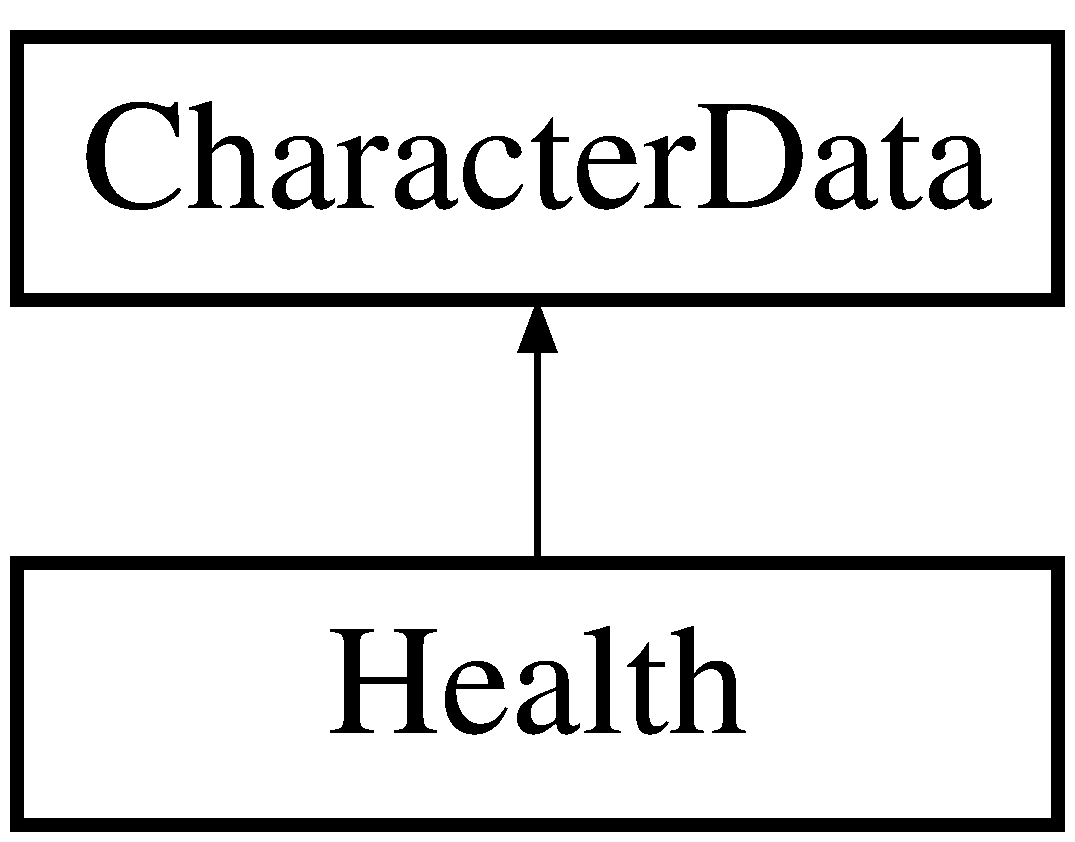
\includegraphics[height=2.000000cm]{struct_health}
\end{center}
\end{figure}
\subsection*{Public Member Functions}
\begin{DoxyCompactItemize}
\item 
\hyperlink{struct_health_acd41f307cc9a942c3335480420c0ace7}{Health} ()
\item 
\hyperlink{struct_health_a0eea3e266fb44e83dc46d6c45430eff5}{Health} (long b)
\item 
\hyperlink{struct_health_a8e581ca46b7ec906bad62ce2144c93a1}{Health} (unsigned long b, unsigned m)
\item 
\hyperlink{struct_health_a87dacc9b041b0fc213f108ca94969817}{Health} (const \hyperlink{struct_health}{Health} \&other)
\end{DoxyCompactItemize}
\subsection*{Additional Inherited Members}


\subsection{Detailed Description}
A data structure that will hold health values 

Definition at line 175 of file Character\-Data.\-h.



\subsection{Constructor \& Destructor Documentation}
\hypertarget{struct_health_acd41f307cc9a942c3335480420c0ace7}{\index{Health@{Health}!Health@{Health}}
\index{Health@{Health}!Health@{Health}}
\subsubsection[{Health}]{\setlength{\rightskip}{0pt plus 5cm}Health\-::\-Health (
\begin{DoxyParamCaption}
{}
\end{DoxyParamCaption}
)\hspace{0.3cm}{\ttfamily [inline]}}}\label{struct_health_acd41f307cc9a942c3335480420c0ace7}


Definition at line 179 of file Character\-Data.\-h.

\hypertarget{struct_health_a0eea3e266fb44e83dc46d6c45430eff5}{\index{Health@{Health}!Health@{Health}}
\index{Health@{Health}!Health@{Health}}
\subsubsection[{Health}]{\setlength{\rightskip}{0pt plus 5cm}Health\-::\-Health (
\begin{DoxyParamCaption}
\item[{long}]{b}
\end{DoxyParamCaption}
)\hspace{0.3cm}{\ttfamily [inline]}}}\label{struct_health_a0eea3e266fb44e83dc46d6c45430eff5}


Definition at line 182 of file Character\-Data.\-h.

\hypertarget{struct_health_a8e581ca46b7ec906bad62ce2144c93a1}{\index{Health@{Health}!Health@{Health}}
\index{Health@{Health}!Health@{Health}}
\subsubsection[{Health}]{\setlength{\rightskip}{0pt plus 5cm}Health\-::\-Health (
\begin{DoxyParamCaption}
\item[{unsigned long}]{b, }
\item[{unsigned}]{m}
\end{DoxyParamCaption}
)\hspace{0.3cm}{\ttfamily [inline]}}}\label{struct_health_a8e581ca46b7ec906bad62ce2144c93a1}


Definition at line 185 of file Character\-Data.\-h.

\hypertarget{struct_health_a87dacc9b041b0fc213f108ca94969817}{\index{Health@{Health}!Health@{Health}}
\index{Health@{Health}!Health@{Health}}
\subsubsection[{Health}]{\setlength{\rightskip}{0pt plus 5cm}Health\-::\-Health (
\begin{DoxyParamCaption}
\item[{const {\bf Health} \&}]{other}
\end{DoxyParamCaption}
)\hspace{0.3cm}{\ttfamily [inline]}}}\label{struct_health_a87dacc9b041b0fc213f108ca94969817}


Definition at line 188 of file Character\-Data.\-h.



The documentation for this struct was generated from the following file\-:\begin{DoxyCompactItemize}
\item 
/\-Volumes/\-O\-S X H\-D\-D/\-Users/\-Adam/\-Developer/\-Sprite\-Fight/\-World/\hyperlink{_character_data_8h}{Character\-Data.\-h}\end{DoxyCompactItemize}

\hypertarget{class_input_controller}{\section{Input\-Controller Class Reference}
\label{class_input_controller}\index{Input\-Controller@{Input\-Controller}}
}


{\ttfamily \#include $<$Input.\-hpp$>$}

\subsection*{Static Public Member Functions}
\begin{DoxyCompactItemize}
\item 
static void \hyperlink{class_input_controller_a34126fbb3541313ed0b1b3eaddb0f9e7}{register\-For\-Event} (\hyperlink{class_event_register}{Event\-Register} $\ast$reg)
\item 
static void \hyperlink{class_input_controller_a0b9059be3b8f5cf7dc60bd295ffe205e}{register\-For\-Keypress} (\hyperlink{class_key_input_register}{Key\-Input\-Register} $\ast$reg)
\item 
{\footnotesize template$<$typename T $>$ }\\static void \hyperlink{class_input_controller_a3fdf7b5696eae64b76d540b35cbc94c7}{register\-For} (T $\ast$event\-\_\-or\-\_\-keypress)
\item 
static void \hyperlink{class_input_controller_a995431661911a85ae39f1591932e4e20}{deregister} (\hyperlink{class_game_interface}{Game\-Interface} $\ast$registered\-Object)
\item 
static void \hyperlink{class_input_controller_aa12eb24fffc0010eb4101c56d0b06dc5}{init} ()
\item 
static void \hyperlink{class_input_controller_ab7e7e742d0b250effa849ed2581e2eb2}{update} ()
\item 
static void \hyperlink{class_input_controller_a95e9c9c2be3a581d4e10fff159007c68}{exit} ()
\end{DoxyCompactItemize}
\subsection*{Protected Member Functions}
\begin{DoxyCompactItemize}
\item 
\hyperlink{class_input_controller_aba927fffeb0bf4c4fd0835d4dfbdfaec}{Input\-Controller} ()
\end{DoxyCompactItemize}
\subsection*{Static Protected Member Functions}
\begin{DoxyCompactItemize}
\item 
static void \hyperlink{class_input_controller_a1e87ceb31ecdcd8bb0ee1af102b20c8a}{listen\-For\-Keypress} ()
\item 
static void \hyperlink{class_input_controller_a550227f0a95207f5361354135e80d191}{listen\-For\-Events} ()
\end{DoxyCompactItemize}
\subsection*{Static Protected Attributes}
\begin{DoxyCompactItemize}
\item 
static vector$<$ \hyperlink{class_event_register}{Event\-Register} $\ast$ $>$ $\ast$ \hyperlink{class_input_controller_afe327cb5fda23f106b0614d9119b1714}{event\-Listener\-Registry} = new vector$<$\hyperlink{class_event_register}{Event\-Register} $\ast$$>$()
\item 
static vector\\*
$<$ \hyperlink{class_key_input_register}{Key\-Input\-Register} $\ast$ $>$ $\ast$ \hyperlink{class_input_controller_a2e26dc4af1946fa78c817f2bd3f4a319}{key\-Input\-Registry} = new vector$<$\hyperlink{class_key_input_register}{Key\-Input\-Register} $\ast$$>$()
\item 
static \hyperlink{_input_8hpp_a968dbade547d18c0fc972caf39d984e8}{Event} $\ast$ \hyperlink{class_input_controller_aa88d822c29ba14ed6fc2b35f171161ce}{event} = (\hyperlink{_input_8hpp_a968dbade547d18c0fc972caf39d984e8}{Event} $\ast$) malloc(sizeof(\hyperlink{_input_8hpp_a968dbade547d18c0fc972caf39d984e8}{Event}))
\item 
static const unsigned char $\ast$ \hyperlink{class_input_controller_a17d54f67ffd783a8fca81a94a6de02e7}{keys}
\item 
static int \hyperlink{class_input_controller_a95bfc98ab2e37c9772b678e9b561c97d}{key\-Array\-Size} = 1
\end{DoxyCompactItemize}


\subsection{Detailed Description}


Definition at line 373 of file Input.\-hpp.



\subsection{Constructor \& Destructor Documentation}
\hypertarget{class_input_controller_aba927fffeb0bf4c4fd0835d4dfbdfaec}{\index{Input\-Controller@{Input\-Controller}!Input\-Controller@{Input\-Controller}}
\index{Input\-Controller@{Input\-Controller}!InputController@{Input\-Controller}}
\subsubsection[{Input\-Controller}]{\setlength{\rightskip}{0pt plus 5cm}Input\-Controller\-::\-Input\-Controller (
\begin{DoxyParamCaption}
{}
\end{DoxyParamCaption}
)\hspace{0.3cm}{\ttfamily [protected]}}}\label{class_input_controller_aba927fffeb0bf4c4fd0835d4dfbdfaec}


\subsection{Member Function Documentation}
\hypertarget{class_input_controller_a995431661911a85ae39f1591932e4e20}{\index{Input\-Controller@{Input\-Controller}!deregister@{deregister}}
\index{deregister@{deregister}!InputController@{Input\-Controller}}
\subsubsection[{deregister}]{\setlength{\rightskip}{0pt plus 5cm}void Input\-Controller\-::deregister (
\begin{DoxyParamCaption}
\item[{{\bf Game\-Interface} $\ast$}]{registered\-Object}
\end{DoxyParamCaption}
)\hspace{0.3cm}{\ttfamily [static]}}}\label{class_input_controller_a995431661911a85ae39f1591932e4e20}


Definition at line 131 of file Input.\-cpp.

\hypertarget{class_input_controller_a95e9c9c2be3a581d4e10fff159007c68}{\index{Input\-Controller@{Input\-Controller}!exit@{exit}}
\index{exit@{exit}!InputController@{Input\-Controller}}
\subsubsection[{exit}]{\setlength{\rightskip}{0pt plus 5cm}void Input\-Controller\-::exit (
\begin{DoxyParamCaption}
{}
\end{DoxyParamCaption}
)\hspace{0.3cm}{\ttfamily [static]}}}\label{class_input_controller_a95e9c9c2be3a581d4e10fff159007c68}


Definition at line 152 of file Input.\-cpp.

\hypertarget{class_input_controller_aa12eb24fffc0010eb4101c56d0b06dc5}{\index{Input\-Controller@{Input\-Controller}!init@{init}}
\index{init@{init}!InputController@{Input\-Controller}}
\subsubsection[{init}]{\setlength{\rightskip}{0pt plus 5cm}void Input\-Controller\-::init (
\begin{DoxyParamCaption}
{}
\end{DoxyParamCaption}
)\hspace{0.3cm}{\ttfamily [static]}}}\label{class_input_controller_aa12eb24fffc0010eb4101c56d0b06dc5}


Definition at line 100 of file Input.\-cpp.

\hypertarget{class_input_controller_a550227f0a95207f5361354135e80d191}{\index{Input\-Controller@{Input\-Controller}!listen\-For\-Events@{listen\-For\-Events}}
\index{listen\-For\-Events@{listen\-For\-Events}!InputController@{Input\-Controller}}
\subsubsection[{listen\-For\-Events}]{\setlength{\rightskip}{0pt plus 5cm}void Input\-Controller\-::listen\-For\-Events (
\begin{DoxyParamCaption}
{}
\end{DoxyParamCaption}
)\hspace{0.3cm}{\ttfamily [static]}, {\ttfamily [protected]}}}\label{class_input_controller_a550227f0a95207f5361354135e80d191}


Definition at line 79 of file Input.\-cpp.

\hypertarget{class_input_controller_a1e87ceb31ecdcd8bb0ee1af102b20c8a}{\index{Input\-Controller@{Input\-Controller}!listen\-For\-Keypress@{listen\-For\-Keypress}}
\index{listen\-For\-Keypress@{listen\-For\-Keypress}!InputController@{Input\-Controller}}
\subsubsection[{listen\-For\-Keypress}]{\setlength{\rightskip}{0pt plus 5cm}void Input\-Controller\-::listen\-For\-Keypress (
\begin{DoxyParamCaption}
{}
\end{DoxyParamCaption}
)\hspace{0.3cm}{\ttfamily [static]}, {\ttfamily [protected]}}}\label{class_input_controller_a1e87ceb31ecdcd8bb0ee1af102b20c8a}


Definition at line 90 of file Input.\-cpp.

\hypertarget{class_input_controller_a3fdf7b5696eae64b76d540b35cbc94c7}{\index{Input\-Controller@{Input\-Controller}!register\-For@{register\-For}}
\index{register\-For@{register\-For}!InputController@{Input\-Controller}}
\subsubsection[{register\-For}]{\setlength{\rightskip}{0pt plus 5cm}template$<$typename T $>$ static void Input\-Controller\-::register\-For (
\begin{DoxyParamCaption}
\item[{T $\ast$}]{event\-\_\-or\-\_\-keypress}
\end{DoxyParamCaption}
)\hspace{0.3cm}{\ttfamily [static]}}}\label{class_input_controller_a3fdf7b5696eae64b76d540b35cbc94c7}
\hypertarget{class_input_controller_a34126fbb3541313ed0b1b3eaddb0f9e7}{\index{Input\-Controller@{Input\-Controller}!register\-For\-Event@{register\-For\-Event}}
\index{register\-For\-Event@{register\-For\-Event}!InputController@{Input\-Controller}}
\subsubsection[{register\-For\-Event}]{\setlength{\rightskip}{0pt plus 5cm}void Input\-Controller\-::register\-For\-Event (
\begin{DoxyParamCaption}
\item[{{\bf Event\-Register} $\ast$}]{reg}
\end{DoxyParamCaption}
)\hspace{0.3cm}{\ttfamily [static]}}}\label{class_input_controller_a34126fbb3541313ed0b1b3eaddb0f9e7}


Definition at line 117 of file Input.\-cpp.

\hypertarget{class_input_controller_a0b9059be3b8f5cf7dc60bd295ffe205e}{\index{Input\-Controller@{Input\-Controller}!register\-For\-Keypress@{register\-For\-Keypress}}
\index{register\-For\-Keypress@{register\-For\-Keypress}!InputController@{Input\-Controller}}
\subsubsection[{register\-For\-Keypress}]{\setlength{\rightskip}{0pt plus 5cm}void Input\-Controller\-::register\-For\-Keypress (
\begin{DoxyParamCaption}
\item[{{\bf Key\-Input\-Register} $\ast$}]{reg}
\end{DoxyParamCaption}
)\hspace{0.3cm}{\ttfamily [static]}}}\label{class_input_controller_a0b9059be3b8f5cf7dc60bd295ffe205e}


Definition at line 121 of file Input.\-cpp.

\hypertarget{class_input_controller_ab7e7e742d0b250effa849ed2581e2eb2}{\index{Input\-Controller@{Input\-Controller}!update@{update}}
\index{update@{update}!InputController@{Input\-Controller}}
\subsubsection[{update}]{\setlength{\rightskip}{0pt plus 5cm}void Input\-Controller\-::update (
\begin{DoxyParamCaption}
{}
\end{DoxyParamCaption}
)\hspace{0.3cm}{\ttfamily [static]}}}\label{class_input_controller_ab7e7e742d0b250effa849ed2581e2eb2}


Definition at line 146 of file Input.\-cpp.



\subsection{Member Data Documentation}
\hypertarget{class_input_controller_aa88d822c29ba14ed6fc2b35f171161ce}{\index{Input\-Controller@{Input\-Controller}!event@{event}}
\index{event@{event}!InputController@{Input\-Controller}}
\subsubsection[{event}]{\setlength{\rightskip}{0pt plus 5cm}{\bf Event} $\ast$ Input\-Controller\-::event = ({\bf Event} $\ast$) malloc(sizeof({\bf Event}))\hspace{0.3cm}{\ttfamily [static]}, {\ttfamily [protected]}}}\label{class_input_controller_aa88d822c29ba14ed6fc2b35f171161ce}


Definition at line 387 of file Input.\-hpp.

\hypertarget{class_input_controller_afe327cb5fda23f106b0614d9119b1714}{\index{Input\-Controller@{Input\-Controller}!event\-Listener\-Registry@{event\-Listener\-Registry}}
\index{event\-Listener\-Registry@{event\-Listener\-Registry}!InputController@{Input\-Controller}}
\subsubsection[{event\-Listener\-Registry}]{\setlength{\rightskip}{0pt plus 5cm}vector$<$ {\bf Event\-Register} $\ast$ $>$ $\ast$ Input\-Controller\-::event\-Listener\-Registry = new vector$<${\bf Event\-Register} $\ast$$>$()\hspace{0.3cm}{\ttfamily [static]}, {\ttfamily [protected]}}}\label{class_input_controller_afe327cb5fda23f106b0614d9119b1714}
Associates keys with callback functions. 

Definition at line 380 of file Input.\-hpp.

\hypertarget{class_input_controller_a95bfc98ab2e37c9772b678e9b561c97d}{\index{Input\-Controller@{Input\-Controller}!key\-Array\-Size@{key\-Array\-Size}}
\index{key\-Array\-Size@{key\-Array\-Size}!InputController@{Input\-Controller}}
\subsubsection[{key\-Array\-Size}]{\setlength{\rightskip}{0pt plus 5cm}int Input\-Controller\-::key\-Array\-Size = 1\hspace{0.3cm}{\ttfamily [static]}, {\ttfamily [protected]}}}\label{class_input_controller_a95bfc98ab2e37c9772b678e9b561c97d}


Definition at line 393 of file Input.\-hpp.

\hypertarget{class_input_controller_a2e26dc4af1946fa78c817f2bd3f4a319}{\index{Input\-Controller@{Input\-Controller}!key\-Input\-Registry@{key\-Input\-Registry}}
\index{key\-Input\-Registry@{key\-Input\-Registry}!InputController@{Input\-Controller}}
\subsubsection[{key\-Input\-Registry}]{\setlength{\rightskip}{0pt plus 5cm}vector$<$ {\bf Key\-Input\-Register} $\ast$ $>$ $\ast$ Input\-Controller\-::key\-Input\-Registry = new vector$<${\bf Key\-Input\-Register} $\ast$$>$()\hspace{0.3cm}{\ttfamily [static]}, {\ttfamily [protected]}}}\label{class_input_controller_a2e26dc4af1946fa78c817f2bd3f4a319}
Associates keys with callback functions. 

Definition at line 385 of file Input.\-hpp.

\hypertarget{class_input_controller_a17d54f67ffd783a8fca81a94a6de02e7}{\index{Input\-Controller@{Input\-Controller}!keys@{keys}}
\index{keys@{keys}!InputController@{Input\-Controller}}
\subsubsection[{keys}]{\setlength{\rightskip}{0pt plus 5cm}const unsigned char $\ast$ Input\-Controller\-::keys\hspace{0.3cm}{\ttfamily [static]}, {\ttfamily [protected]}}}\label{class_input_controller_a17d54f67ffd783a8fca81a94a6de02e7}
Holds pointers to the state of each key on the keyboard. Initialized once, but valid for the scope of the program. 

Definition at line 392 of file Input.\-hpp.



The documentation for this class was generated from the following files\-:\begin{DoxyCompactItemize}
\item 
/\-Volumes/\-O\-S X H\-D\-D/\-Users/\-Adam/\-Developer/\-Sprite\-Fight/\-Control/\hyperlink{_input_8hpp}{Input.\-hpp}\item 
/\-Volumes/\-O\-S X H\-D\-D/\-Users/\-Adam/\-Developer/\-Sprite\-Fight/\-Control/\hyperlink{_input_8cpp}{Input.\-cpp}\end{DoxyCompactItemize}

\hypertarget{class_key_input_register}{\section{Key\-Input\-Register Class Reference}
\label{class_key_input_register}\index{Key\-Input\-Register@{Key\-Input\-Register}}
}


{\ttfamily \#include $<$Input.\-hpp$>$}

Inheritance diagram for Key\-Input\-Register\-:\begin{figure}[H]
\begin{center}
\leavevmode
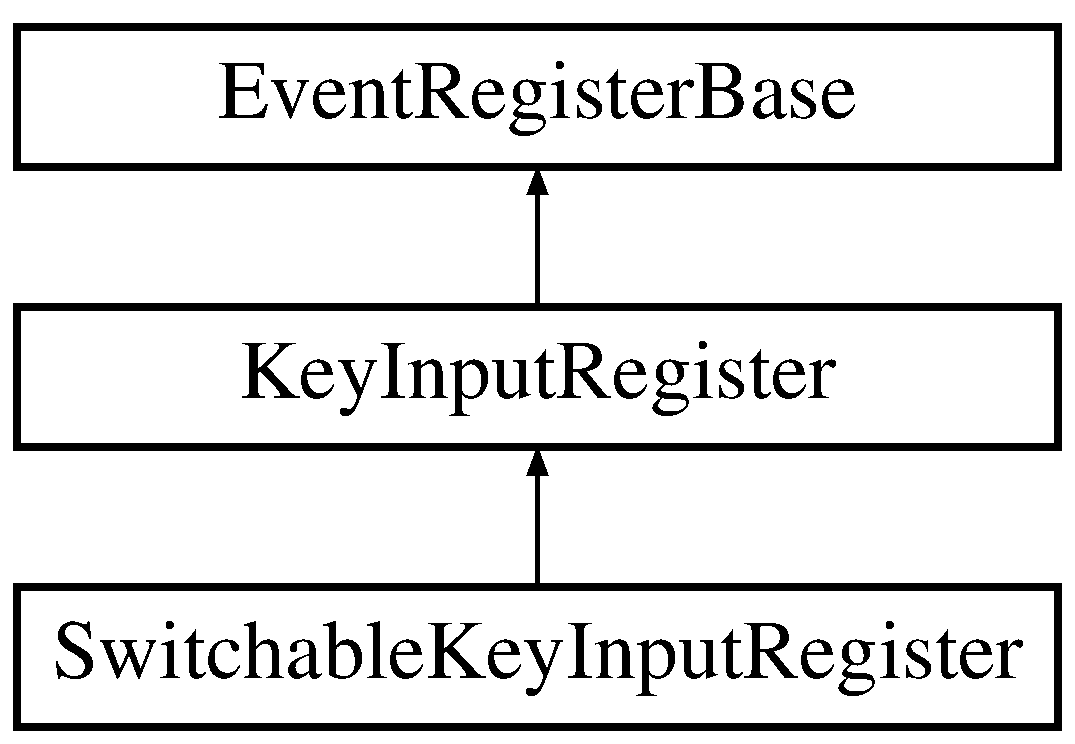
\includegraphics[height=3.000000cm]{class_key_input_register}
\end{center}
\end{figure}
\subsection*{Public Member Functions}
\begin{DoxyCompactItemize}
\item 
\hyperlink{class_key_input_register_a6a51b43c1ceadda862deed824456434e}{Key\-Input\-Register} ()
\item 
\hyperlink{class_key_input_register_ac0c481b0e43fdad2965d547477412a89}{Key\-Input\-Register} (const \hyperlink{class_key_input_register}{Key\-Input\-Register} \&other)
\item 
\hyperlink{class_key_input_register_a965d3c77c5f5edd8a6e376cd8bf0a55f}{Key\-Input\-Register} (\hyperlink{class_key_input_register}{Key\-Input\-Register} \&\&other)
\item 
\hyperlink{class_key_input_register_a19aa82ae77df55f40f3fcbbf37d6e78a}{Key\-Input\-Register} (\hyperlink{class_game_interface}{Game\-Interface} $\ast$call\-On, void(Game\-Interface\-::$\ast$cb)(), initializer\-\_\-list$<$ string $>$ key\-Char, \hyperlink{_input_8hpp_ac32d0351518cb71146a1cd777bc4fc91}{Keypress\-Evaluation\-Method} m)
\item 
{\footnotesize template$<$class T $>$ }\\\hyperlink{class_key_input_register_aa4e8032393db889d4835183891b4a4f5}{Key\-Input\-Register} (\hyperlink{class_game_interface}{Game\-Interface} $\ast$call\-On, void(Game\-Interface\-::$\ast$cb)(), T $\ast$arg0, initializer\-\_\-list$<$ string $>$ key\-Char, \hyperlink{_input_8hpp_ac32d0351518cb71146a1cd777bc4fc91}{Keypress\-Evaluation\-Method} m)
\item 
\hyperlink{class_key_input_register_a2fd8e4aeb3e624f4c6f86ba34481c4ee}{Key\-Input\-Register} (function$<$ void(void)$>$ cb, initializer\-\_\-list$<$ string $>$ key\-Char, \hyperlink{_input_8hpp_ac32d0351518cb71146a1cd777bc4fc91}{Keypress\-Evaluation\-Method} m)
\item 
\hyperlink{class_key_input_register_a261ad3b9948e06fb843459393ee2489f}{Key\-Input\-Register} (\hyperlink{class_game_interface}{Game\-Interface} $\ast$call\-On, void(Game\-Interface\-::$\ast$cb)(), initializer\-\_\-list$<$ \hyperlink{_input_8hpp_ad39c2e59d8cf6782d7ab90b73c0d0ada}{Key\-Code} $>$ key\-Code, \hyperlink{_input_8hpp_ac32d0351518cb71146a1cd777bc4fc91}{Keypress\-Evaluation\-Method} m)
\item 
\hyperlink{class_key_input_register_a27e34e2fc96aa8b92583c1dca8dcb0e7}{Key\-Input\-Register} (function$<$ void(void)$>$ cb, initializer\-\_\-list$<$ \hyperlink{_input_8hpp_ad39c2e59d8cf6782d7ab90b73c0d0ada}{Key\-Code} $>$ key\-Code)
\item 
\hyperlink{class_key_input_register_abe0349140084c11d90cdf3f56278407f}{Key\-Input\-Register} (\hyperlink{class_game_interface}{Game\-Interface} $\ast$call\-On, void(Game\-Interface\-::$\ast$cb)(), initializer\-\_\-list$<$ string $>$ key\-Char, initializer\-\_\-list$<$ \hyperlink{_input_8hpp_ad39c2e59d8cf6782d7ab90b73c0d0ada}{Key\-Code} $>$ key\-Code, \hyperlink{_input_8hpp_ac32d0351518cb71146a1cd777bc4fc91}{Keypress\-Evaluation\-Method} m)
\item 
\hyperlink{class_key_input_register_a255b4fcfd7ff93d8c81c4963dc77d424}{Key\-Input\-Register} (function$<$ void(void)$>$ cb, initializer\-\_\-list$<$ string $>$ key\-Char, initializer\-\_\-list$<$ \hyperlink{_input_8hpp_ad39c2e59d8cf6782d7ab90b73c0d0ada}{Key\-Code} $>$ key\-Code, \hyperlink{_input_8hpp_ac32d0351518cb71146a1cd777bc4fc91}{Keypress\-Evaluation\-Method} m)
\item 
\hyperlink{class_key_input_register_a5c01a99075e25878f2cb673d6341861b}{$\sim$\-Key\-Input\-Register} ()
\end{DoxyCompactItemize}
\subsection*{Static Public Member Functions}
\begin{DoxyCompactItemize}
\item 
static \hyperlink{_input_8hpp_ab11de2748648ed8559e324a4b8dfb2da}{Scan\-Code} \hyperlink{class_key_input_register_a439b37fd3322d8957aa95d9775550db5}{get\-Scan\-Code\-For} (const char $\ast$c)
\item 
static \hyperlink{_input_8hpp_ab11de2748648ed8559e324a4b8dfb2da}{Scan\-Code} \hyperlink{class_key_input_register_a4f8b4b7572911432931bf6bd835f52ef}{get\-Scan\-Code\-For} (\hyperlink{_input_8hpp_ad39c2e59d8cf6782d7ab90b73c0d0ada}{Key\-Code} code)
\end{DoxyCompactItemize}
\subsection*{Protected Types}
\begin{DoxyCompactItemize}
\item 
enum \hyperlink{class_key_input_register_a21a7be17fdf11de9736f801ed23b3d5d}{Key\-Iden\-Method} \{ \hyperlink{class_key_input_register_a21a7be17fdf11de9736f801ed23b3d5dacf1e24867419a579f668008e39431010}{Key\-Iden\-Method\-::key\-Char} = 0, 
\hyperlink{class_key_input_register_a21a7be17fdf11de9736f801ed23b3d5dab96beb1fb95f7fa45257bb48942aef8a}{Key\-Iden\-Method\-::key\-Code} = 1, 
\hyperlink{class_key_input_register_a21a7be17fdf11de9736f801ed23b3d5daf6cb3e816496528d4187db53bc66567f}{Key\-Iden\-Method\-::both} = (key\-Char \& key\-Code)
 \}
\end{DoxyCompactItemize}
\subsection*{Protected Member Functions}
\begin{DoxyCompactItemize}
\item 
bool \hyperlink{class_key_input_register_a0e5993cb2e93f288a4acf7d34da6edad}{check\-For\-Pressed\-Keys} (const unsigned char $\ast$keyboard\-State, vector$<$ \hyperlink{_input_8hpp_ab11de2748648ed8559e324a4b8dfb2da}{Scan\-Code} $>$\-::iterator scan\-Code)
\item 
virtual void \hyperlink{class_key_input_register_a076a886cd83efe7d7aaa11f670d75e61}{handle\-Keyboard\-Input} (const unsigned char $\ast$keyboard\-State)
\end{DoxyCompactItemize}
\subsection*{Protected Attributes}
\begin{DoxyCompactItemize}
\item 
vector$<$ \hyperlink{_input_8hpp_ab11de2748648ed8559e324a4b8dfb2da}{Scan\-Code} $>$ \hyperlink{class_key_input_register_abc2af3b54d196eda9e64fdcd6da118d0}{scan\-Codes}
\item 
vector$<$ string $>$ \hyperlink{class_key_input_register_a6ff79253202f3106320ed21e9f3eb803}{requested\-Keyboard\-Chars}
\item 
vector$<$ \hyperlink{_input_8hpp_ad39c2e59d8cf6782d7ab90b73c0d0ada}{Key\-Code} $>$ \hyperlink{class_key_input_register_a15cc8379e648634a63e1bedd645d03c3}{requested\-Key\-Codes}
\item 
\hyperlink{_input_8hpp_ac32d0351518cb71146a1cd777bc4fc91}{Keypress\-Evaluation\-Method} \hyperlink{class_key_input_register_a99a156d91abafbd8a1f191d15158d1ba}{requested\-Key\-Eval\-Method}
\item 
enum \\*
\hyperlink{class_key_input_register_a21a7be17fdf11de9736f801ed23b3d5d}{Key\-Input\-Register\-::\-Key\-Iden\-Method} \hyperlink{class_key_input_register_adf60b0b21fcd0b52bf3c505528519b47}{key\-I\-D\-Method}
\end{DoxyCompactItemize}
\subsection*{Friends}
\begin{DoxyCompactItemize}
\item 
class \hyperlink{class_key_input_register_a083d5a8d8c2dd3a28d1f55d2965db0ab}{Input\-Controller}
\end{DoxyCompactItemize}


\subsection{Detailed Description}
An implementation of \hyperlink{class_event_register_base}{Event\-Register\-Base} specialized for handling keyboard input. 

Definition at line 175 of file Input.\-hpp.



\subsection{Member Enumeration Documentation}
\hypertarget{class_key_input_register_a21a7be17fdf11de9736f801ed23b3d5d}{\index{Key\-Input\-Register@{Key\-Input\-Register}!Key\-Iden\-Method@{Key\-Iden\-Method}}
\index{Key\-Iden\-Method@{Key\-Iden\-Method}!KeyInputRegister@{Key\-Input\-Register}}
\subsubsection[{Key\-Iden\-Method}]{\setlength{\rightskip}{0pt plus 5cm}enum {\bf Key\-Input\-Register\-::\-Key\-Iden\-Method}\hspace{0.3cm}{\ttfamily [strong]}, {\ttfamily [protected]}}}\label{class_key_input_register_a21a7be17fdf11de9736f801ed23b3d5d}
This enumeration represents whether this \hyperlink{class_key_input_register}{Key\-Input\-Register} references \begin{Desc}
\item[Enumerator]\par
\begin{description}
\index{key\-Char@{key\-Char}!Key\-Input\-Register@{Key\-Input\-Register}}\index{Key\-Input\-Register@{Key\-Input\-Register}!key\-Char@{key\-Char}}\item[{\em 
\hypertarget{class_key_input_register_a21a7be17fdf11de9736f801ed23b3d5dacf1e24867419a579f668008e39431010}{key\-Char}\label{class_key_input_register_a21a7be17fdf11de9736f801ed23b3d5dacf1e24867419a579f668008e39431010}
}]\index{key\-Code@{key\-Code}!Key\-Input\-Register@{Key\-Input\-Register}}\index{Key\-Input\-Register@{Key\-Input\-Register}!key\-Code@{key\-Code}}\item[{\em 
\hypertarget{class_key_input_register_a21a7be17fdf11de9736f801ed23b3d5dab96beb1fb95f7fa45257bb48942aef8a}{key\-Code}\label{class_key_input_register_a21a7be17fdf11de9736f801ed23b3d5dab96beb1fb95f7fa45257bb48942aef8a}
}]\index{both@{both}!Key\-Input\-Register@{Key\-Input\-Register}}\index{Key\-Input\-Register@{Key\-Input\-Register}!both@{both}}\item[{\em 
\hypertarget{class_key_input_register_a21a7be17fdf11de9736f801ed23b3d5daf6cb3e816496528d4187db53bc66567f}{both}\label{class_key_input_register_a21a7be17fdf11de9736f801ed23b3d5daf6cb3e816496528d4187db53bc66567f}
}]\end{description}
\end{Desc}


Definition at line 194 of file Input.\-hpp.



\subsection{Constructor \& Destructor Documentation}
\hypertarget{class_key_input_register_a6a51b43c1ceadda862deed824456434e}{\index{Key\-Input\-Register@{Key\-Input\-Register}!Key\-Input\-Register@{Key\-Input\-Register}}
\index{Key\-Input\-Register@{Key\-Input\-Register}!KeyInputRegister@{Key\-Input\-Register}}
\subsubsection[{Key\-Input\-Register}]{\setlength{\rightskip}{0pt plus 5cm}Key\-Input\-Register\-::\-Key\-Input\-Register (
\begin{DoxyParamCaption}
{}
\end{DoxyParamCaption}
)\hspace{0.3cm}{\ttfamily [inline]}}}\label{class_key_input_register_a6a51b43c1ceadda862deed824456434e}


Definition at line 212 of file Input.\-hpp.

\hypertarget{class_key_input_register_ac0c481b0e43fdad2965d547477412a89}{\index{Key\-Input\-Register@{Key\-Input\-Register}!Key\-Input\-Register@{Key\-Input\-Register}}
\index{Key\-Input\-Register@{Key\-Input\-Register}!KeyInputRegister@{Key\-Input\-Register}}
\subsubsection[{Key\-Input\-Register}]{\setlength{\rightskip}{0pt plus 5cm}Key\-Input\-Register\-::\-Key\-Input\-Register (
\begin{DoxyParamCaption}
\item[{const {\bf Key\-Input\-Register} \&}]{other}
\end{DoxyParamCaption}
)\hspace{0.3cm}{\ttfamily [inline]}}}\label{class_key_input_register_ac0c481b0e43fdad2965d547477412a89}


Definition at line 214 of file Input.\-hpp.

\hypertarget{class_key_input_register_a965d3c77c5f5edd8a6e376cd8bf0a55f}{\index{Key\-Input\-Register@{Key\-Input\-Register}!Key\-Input\-Register@{Key\-Input\-Register}}
\index{Key\-Input\-Register@{Key\-Input\-Register}!KeyInputRegister@{Key\-Input\-Register}}
\subsubsection[{Key\-Input\-Register}]{\setlength{\rightskip}{0pt plus 5cm}Key\-Input\-Register\-::\-Key\-Input\-Register (
\begin{DoxyParamCaption}
\item[{{\bf Key\-Input\-Register} \&\&}]{other}
\end{DoxyParamCaption}
)\hspace{0.3cm}{\ttfamily [inline]}}}\label{class_key_input_register_a965d3c77c5f5edd8a6e376cd8bf0a55f}


Definition at line 235 of file Input.\-hpp.

\hypertarget{class_key_input_register_a19aa82ae77df55f40f3fcbbf37d6e78a}{\index{Key\-Input\-Register@{Key\-Input\-Register}!Key\-Input\-Register@{Key\-Input\-Register}}
\index{Key\-Input\-Register@{Key\-Input\-Register}!KeyInputRegister@{Key\-Input\-Register}}
\subsubsection[{Key\-Input\-Register}]{\setlength{\rightskip}{0pt plus 5cm}Key\-Input\-Register\-::\-Key\-Input\-Register (
\begin{DoxyParamCaption}
\item[{{\bf Game\-Interface} $\ast$}]{call\-On, }
\item[{void(Game\-Interface\-::$\ast$)()}]{cb, }
\item[{initializer\-\_\-list$<$ string $>$}]{key\-Char, }
\item[{{\bf Keypress\-Evaluation\-Method}}]{m}
\end{DoxyParamCaption}
)\hspace{0.3cm}{\ttfamily [inline]}}}\label{class_key_input_register_a19aa82ae77df55f40f3fcbbf37d6e78a}


Definition at line 243 of file Input.\-hpp.

\hypertarget{class_key_input_register_aa4e8032393db889d4835183891b4a4f5}{\index{Key\-Input\-Register@{Key\-Input\-Register}!Key\-Input\-Register@{Key\-Input\-Register}}
\index{Key\-Input\-Register@{Key\-Input\-Register}!KeyInputRegister@{Key\-Input\-Register}}
\subsubsection[{Key\-Input\-Register}]{\setlength{\rightskip}{0pt plus 5cm}template$<$class T $>$ Key\-Input\-Register\-::\-Key\-Input\-Register (
\begin{DoxyParamCaption}
\item[{{\bf Game\-Interface} $\ast$}]{call\-On, }
\item[{void(Game\-Interface\-::$\ast$)()}]{cb, }
\item[{T $\ast$}]{arg0, }
\item[{initializer\-\_\-list$<$ string $>$}]{key\-Char, }
\item[{{\bf Keypress\-Evaluation\-Method}}]{m}
\end{DoxyParamCaption}
)\hspace{0.3cm}{\ttfamily [inline]}}}\label{class_key_input_register_aa4e8032393db889d4835183891b4a4f5}


Definition at line 257 of file Input.\-hpp.

\hypertarget{class_key_input_register_a2fd8e4aeb3e624f4c6f86ba34481c4ee}{\index{Key\-Input\-Register@{Key\-Input\-Register}!Key\-Input\-Register@{Key\-Input\-Register}}
\index{Key\-Input\-Register@{Key\-Input\-Register}!KeyInputRegister@{Key\-Input\-Register}}
\subsubsection[{Key\-Input\-Register}]{\setlength{\rightskip}{0pt plus 5cm}Key\-Input\-Register\-::\-Key\-Input\-Register (
\begin{DoxyParamCaption}
\item[{function$<$ void(void)$>$}]{cb, }
\item[{initializer\-\_\-list$<$ string $>$}]{key\-Char, }
\item[{{\bf Keypress\-Evaluation\-Method}}]{m}
\end{DoxyParamCaption}
)\hspace{0.3cm}{\ttfamily [inline]}}}\label{class_key_input_register_a2fd8e4aeb3e624f4c6f86ba34481c4ee}


Definition at line 270 of file Input.\-hpp.

\hypertarget{class_key_input_register_a261ad3b9948e06fb843459393ee2489f}{\index{Key\-Input\-Register@{Key\-Input\-Register}!Key\-Input\-Register@{Key\-Input\-Register}}
\index{Key\-Input\-Register@{Key\-Input\-Register}!KeyInputRegister@{Key\-Input\-Register}}
\subsubsection[{Key\-Input\-Register}]{\setlength{\rightskip}{0pt plus 5cm}Key\-Input\-Register\-::\-Key\-Input\-Register (
\begin{DoxyParamCaption}
\item[{{\bf Game\-Interface} $\ast$}]{call\-On, }
\item[{void(Game\-Interface\-::$\ast$)()}]{cb, }
\item[{initializer\-\_\-list$<$ {\bf Key\-Code} $>$}]{key\-Code, }
\item[{{\bf Keypress\-Evaluation\-Method}}]{m}
\end{DoxyParamCaption}
)\hspace{0.3cm}{\ttfamily [inline]}}}\label{class_key_input_register_a261ad3b9948e06fb843459393ee2489f}


Definition at line 283 of file Input.\-hpp.

\hypertarget{class_key_input_register_a27e34e2fc96aa8b92583c1dca8dcb0e7}{\index{Key\-Input\-Register@{Key\-Input\-Register}!Key\-Input\-Register@{Key\-Input\-Register}}
\index{Key\-Input\-Register@{Key\-Input\-Register}!KeyInputRegister@{Key\-Input\-Register}}
\subsubsection[{Key\-Input\-Register}]{\setlength{\rightskip}{0pt plus 5cm}Key\-Input\-Register\-::\-Key\-Input\-Register (
\begin{DoxyParamCaption}
\item[{function$<$ void(void)$>$}]{cb, }
\item[{initializer\-\_\-list$<$ {\bf Key\-Code} $>$}]{key\-Code}
\end{DoxyParamCaption}
)\hspace{0.3cm}{\ttfamily [inline]}}}\label{class_key_input_register_a27e34e2fc96aa8b92583c1dca8dcb0e7}


Definition at line 296 of file Input.\-hpp.

\hypertarget{class_key_input_register_abe0349140084c11d90cdf3f56278407f}{\index{Key\-Input\-Register@{Key\-Input\-Register}!Key\-Input\-Register@{Key\-Input\-Register}}
\index{Key\-Input\-Register@{Key\-Input\-Register}!KeyInputRegister@{Key\-Input\-Register}}
\subsubsection[{Key\-Input\-Register}]{\setlength{\rightskip}{0pt plus 5cm}Key\-Input\-Register\-::\-Key\-Input\-Register (
\begin{DoxyParamCaption}
\item[{{\bf Game\-Interface} $\ast$}]{call\-On, }
\item[{void(Game\-Interface\-::$\ast$)()}]{cb, }
\item[{initializer\-\_\-list$<$ string $>$}]{key\-Char, }
\item[{initializer\-\_\-list$<$ {\bf Key\-Code} $>$}]{key\-Code, }
\item[{{\bf Keypress\-Evaluation\-Method}}]{m}
\end{DoxyParamCaption}
)\hspace{0.3cm}{\ttfamily [inline]}}}\label{class_key_input_register_abe0349140084c11d90cdf3f56278407f}


Definition at line 308 of file Input.\-hpp.

\hypertarget{class_key_input_register_a255b4fcfd7ff93d8c81c4963dc77d424}{\index{Key\-Input\-Register@{Key\-Input\-Register}!Key\-Input\-Register@{Key\-Input\-Register}}
\index{Key\-Input\-Register@{Key\-Input\-Register}!KeyInputRegister@{Key\-Input\-Register}}
\subsubsection[{Key\-Input\-Register}]{\setlength{\rightskip}{0pt plus 5cm}Key\-Input\-Register\-::\-Key\-Input\-Register (
\begin{DoxyParamCaption}
\item[{function$<$ void(void)$>$}]{cb, }
\item[{initializer\-\_\-list$<$ string $>$}]{key\-Char, }
\item[{initializer\-\_\-list$<$ {\bf Key\-Code} $>$}]{key\-Code, }
\item[{{\bf Keypress\-Evaluation\-Method}}]{m}
\end{DoxyParamCaption}
)\hspace{0.3cm}{\ttfamily [inline]}}}\label{class_key_input_register_a255b4fcfd7ff93d8c81c4963dc77d424}


Definition at line 328 of file Input.\-hpp.

\hypertarget{class_key_input_register_a5c01a99075e25878f2cb673d6341861b}{\index{Key\-Input\-Register@{Key\-Input\-Register}!$\sim$\-Key\-Input\-Register@{$\sim$\-Key\-Input\-Register}}
\index{$\sim$\-Key\-Input\-Register@{$\sim$\-Key\-Input\-Register}!KeyInputRegister@{Key\-Input\-Register}}
\subsubsection[{$\sim$\-Key\-Input\-Register}]{\setlength{\rightskip}{0pt plus 5cm}Key\-Input\-Register\-::$\sim$\-Key\-Input\-Register (
\begin{DoxyParamCaption}
{}
\end{DoxyParamCaption}
)\hspace{0.3cm}{\ttfamily [inline]}}}\label{class_key_input_register_a5c01a99075e25878f2cb673d6341861b}


Definition at line 348 of file Input.\-hpp.



\subsection{Member Function Documentation}
\hypertarget{class_key_input_register_a0e5993cb2e93f288a4acf7d34da6edad}{\index{Key\-Input\-Register@{Key\-Input\-Register}!check\-For\-Pressed\-Keys@{check\-For\-Pressed\-Keys}}
\index{check\-For\-Pressed\-Keys@{check\-For\-Pressed\-Keys}!KeyInputRegister@{Key\-Input\-Register}}
\subsubsection[{check\-For\-Pressed\-Keys}]{\setlength{\rightskip}{0pt plus 5cm}bool Key\-Input\-Register\-::check\-For\-Pressed\-Keys (
\begin{DoxyParamCaption}
\item[{const unsigned char $\ast$}]{keyboard\-State, }
\item[{vector$<$ {\bf Scan\-Code} $>$\-::iterator}]{scan\-Code}
\end{DoxyParamCaption}
)\hspace{0.3cm}{\ttfamily [protected]}}}\label{class_key_input_register_a0e5993cb2e93f288a4acf7d34da6edad}
Recursively checks the keyboard state against all Scan\-Codes corresponding to requested keys, and turns true if all are pressed, or false otherwise. 

Definition at line 32 of file Input.\-cpp.

\hypertarget{class_key_input_register_a439b37fd3322d8957aa95d9775550db5}{\index{Key\-Input\-Register@{Key\-Input\-Register}!get\-Scan\-Code\-For@{get\-Scan\-Code\-For}}
\index{get\-Scan\-Code\-For@{get\-Scan\-Code\-For}!KeyInputRegister@{Key\-Input\-Register}}
\subsubsection[{get\-Scan\-Code\-For}]{\setlength{\rightskip}{0pt plus 5cm}static {\bf Scan\-Code} Key\-Input\-Register\-::get\-Scan\-Code\-For (
\begin{DoxyParamCaption}
\item[{const char $\ast$}]{c}
\end{DoxyParamCaption}
)\hspace{0.3cm}{\ttfamily [inline]}, {\ttfamily [static]}}}\label{class_key_input_register_a439b37fd3322d8957aa95d9775550db5}


Definition at line 350 of file Input.\-hpp.

\hypertarget{class_key_input_register_a4f8b4b7572911432931bf6bd835f52ef}{\index{Key\-Input\-Register@{Key\-Input\-Register}!get\-Scan\-Code\-For@{get\-Scan\-Code\-For}}
\index{get\-Scan\-Code\-For@{get\-Scan\-Code\-For}!KeyInputRegister@{Key\-Input\-Register}}
\subsubsection[{get\-Scan\-Code\-For}]{\setlength{\rightskip}{0pt plus 5cm}static {\bf Scan\-Code} Key\-Input\-Register\-::get\-Scan\-Code\-For (
\begin{DoxyParamCaption}
\item[{{\bf Key\-Code}}]{code}
\end{DoxyParamCaption}
)\hspace{0.3cm}{\ttfamily [inline]}, {\ttfamily [static]}}}\label{class_key_input_register_a4f8b4b7572911432931bf6bd835f52ef}


Definition at line 352 of file Input.\-hpp.

\hypertarget{class_key_input_register_a076a886cd83efe7d7aaa11f670d75e61}{\index{Key\-Input\-Register@{Key\-Input\-Register}!handle\-Keyboard\-Input@{handle\-Keyboard\-Input}}
\index{handle\-Keyboard\-Input@{handle\-Keyboard\-Input}!KeyInputRegister@{Key\-Input\-Register}}
\subsubsection[{handle\-Keyboard\-Input}]{\setlength{\rightskip}{0pt plus 5cm}void Key\-Input\-Register\-::handle\-Keyboard\-Input (
\begin{DoxyParamCaption}
\item[{const unsigned char $\ast$}]{keyboard\-State}
\end{DoxyParamCaption}
)\hspace{0.3cm}{\ttfamily [protected]}, {\ttfamily [virtual]}}}\label{class_key_input_register_a076a886cd83efe7d7aaa11f670d75e61}


Definition at line 62 of file Input.\-cpp.



\subsection{Friends And Related Function Documentation}
\hypertarget{class_key_input_register_a083d5a8d8c2dd3a28d1f55d2965db0ab}{\index{Key\-Input\-Register@{Key\-Input\-Register}!Input\-Controller@{Input\-Controller}}
\index{Input\-Controller@{Input\-Controller}!KeyInputRegister@{Key\-Input\-Register}}
\subsubsection[{Input\-Controller}]{\setlength{\rightskip}{0pt plus 5cm}friend class {\bf Input\-Controller}\hspace{0.3cm}{\ttfamily [friend]}}}\label{class_key_input_register_a083d5a8d8c2dd3a28d1f55d2965db0ab}


Definition at line 208 of file Input.\-hpp.



\subsection{Member Data Documentation}
\hypertarget{class_key_input_register_adf60b0b21fcd0b52bf3c505528519b47}{\index{Key\-Input\-Register@{Key\-Input\-Register}!key\-I\-D\-Method@{key\-I\-D\-Method}}
\index{key\-I\-D\-Method@{key\-I\-D\-Method}!KeyInputRegister@{Key\-Input\-Register}}
\subsubsection[{key\-I\-D\-Method}]{\setlength{\rightskip}{0pt plus 5cm}enum {\bf Key\-Input\-Register\-::\-Key\-Iden\-Method}  Key\-Input\-Register\-::key\-I\-D\-Method\hspace{0.3cm}{\ttfamily [protected]}}}\label{class_key_input_register_adf60b0b21fcd0b52bf3c505528519b47}
\hypertarget{class_key_input_register_a6ff79253202f3106320ed21e9f3eb803}{\index{Key\-Input\-Register@{Key\-Input\-Register}!requested\-Keyboard\-Chars@{requested\-Keyboard\-Chars}}
\index{requested\-Keyboard\-Chars@{requested\-Keyboard\-Chars}!KeyInputRegister@{Key\-Input\-Register}}
\subsubsection[{requested\-Keyboard\-Chars}]{\setlength{\rightskip}{0pt plus 5cm}vector$<$string$>$ Key\-Input\-Register\-::requested\-Keyboard\-Chars\hspace{0.3cm}{\ttfamily [protected]}}}\label{class_key_input_register_a6ff79253202f3106320ed21e9f3eb803}
The string representing the keyboard key the client wishes to listen for 

Definition at line 185 of file Input.\-hpp.

\hypertarget{class_key_input_register_a15cc8379e648634a63e1bedd645d03c3}{\index{Key\-Input\-Register@{Key\-Input\-Register}!requested\-Key\-Codes@{requested\-Key\-Codes}}
\index{requested\-Key\-Codes@{requested\-Key\-Codes}!KeyInputRegister@{Key\-Input\-Register}}
\subsubsection[{requested\-Key\-Codes}]{\setlength{\rightskip}{0pt plus 5cm}vector$<${\bf Key\-Code}$>$ Key\-Input\-Register\-::requested\-Key\-Codes\hspace{0.3cm}{\ttfamily [protected]}}}\label{class_key_input_register_a15cc8379e648634a63e1bedd645d03c3}


Definition at line 187 of file Input.\-hpp.

\hypertarget{class_key_input_register_a99a156d91abafbd8a1f191d15158d1ba}{\index{Key\-Input\-Register@{Key\-Input\-Register}!requested\-Key\-Eval\-Method@{requested\-Key\-Eval\-Method}}
\index{requested\-Key\-Eval\-Method@{requested\-Key\-Eval\-Method}!KeyInputRegister@{Key\-Input\-Register}}
\subsubsection[{requested\-Key\-Eval\-Method}]{\setlength{\rightskip}{0pt plus 5cm}{\bf Keypress\-Evaluation\-Method} Key\-Input\-Register\-::requested\-Key\-Eval\-Method\hspace{0.3cm}{\ttfamily [protected]}}}\label{class_key_input_register_a99a156d91abafbd8a1f191d15158d1ba}


Definition at line 189 of file Input.\-hpp.

\hypertarget{class_key_input_register_abc2af3b54d196eda9e64fdcd6da118d0}{\index{Key\-Input\-Register@{Key\-Input\-Register}!scan\-Codes@{scan\-Codes}}
\index{scan\-Codes@{scan\-Codes}!KeyInputRegister@{Key\-Input\-Register}}
\subsubsection[{scan\-Codes}]{\setlength{\rightskip}{0pt plus 5cm}vector$<${\bf Scan\-Code}$>$ Key\-Input\-Register\-::scan\-Codes\hspace{0.3cm}{\ttfamily [protected]}}}\label{class_key_input_register_abc2af3b54d196eda9e64fdcd6da118d0}


Definition at line 179 of file Input.\-hpp.



The documentation for this class was generated from the following files\-:\begin{DoxyCompactItemize}
\item 
/\-Volumes/\-O\-S X H\-D\-D/\-Users/\-Adam/\-Developer/\-Sprite\-Fight/\-Control/\hyperlink{_input_8hpp}{Input.\-hpp}\item 
/\-Volumes/\-O\-S X H\-D\-D/\-Users/\-Adam/\-Developer/\-Sprite\-Fight/\-Control/\hyperlink{_input_8cpp}{Input.\-cpp}\end{DoxyCompactItemize}

\hypertarget{class_main_controller}{\section{Main\-Controller Class Reference}
\label{class_main_controller}\index{Main\-Controller@{Main\-Controller}}
}


{\ttfamily \#include $<$Main\-Controller.\-h$>$}

\subsection*{Static Public Member Functions}
\begin{DoxyCompactItemize}
\item 
static void \hyperlink{class_main_controller_afb3dbf8d0314f5e5cfe50c703ed4b941}{init} ()
\begin{DoxyCompactList}\small\item\em Initializes the game before \hyperlink{class_main_controller_a98417d12903433cadd2b286bb975905a}{Main\-Controller\-::main()} is called. \end{DoxyCompactList}\item 
static void \hyperlink{class_main_controller_a98417d12903433cadd2b286bb975905a}{main} ()
\end{DoxyCompactItemize}
\subsection*{Static Protected Member Functions}
\begin{DoxyCompactItemize}
\item 
static void \hyperlink{class_main_controller_a04b64137acaa9533edf2eefc941231bf}{begin\-\_\-exit} ()
\item 
static void \hyperlink{class_main_controller_aa81c81c1c28da409b6a527e872d2ab24}{setup\-Main\-Contr\-Exit} ()
\item 
static void \hyperlink{class_main_controller_ad806bb46ae6399a8d0ca0dd1a201a550}{exit} (int sig=0)
\begin{DoxyCompactList}\small\item\em Exits the game. \end{DoxyCompactList}\end{DoxyCompactItemize}
\subsection*{Static Protected Attributes}
\begin{DoxyCompactItemize}
\item 
static \hyperlink{class_player}{Player} $\ast$ \hyperlink{class_main_controller_a778b81dc094ee4409686579d65edb1e4}{player0} = nullptr
\item 
static \hyperlink{class_player}{Player} $\ast$ \hyperlink{class_main_controller_adfc74b59bd82472bd38642e7fa8fd723}{player1} = nullptr
\item 
static const unsigned $\ast$ \hyperlink{class_main_controller_a68d914337e15b04d3160a528bb62fc1f}{loop\-Count} = \&\hyperlink{_game_state_8cpp_afbf04a84d141072dab9bf93db6c9ad29}{main\-Game\-Loop\-Count}
\end{DoxyCompactItemize}


\subsection{Detailed Description}


Definition at line 39 of file Main\-Controller.\-h.



\subsection{Member Function Documentation}
\hypertarget{class_main_controller_a04b64137acaa9533edf2eefc941231bf}{\index{Main\-Controller@{Main\-Controller}!begin\-\_\-exit@{begin\-\_\-exit}}
\index{begin\-\_\-exit@{begin\-\_\-exit}!MainController@{Main\-Controller}}
\subsubsection[{begin\-\_\-exit}]{\setlength{\rightskip}{0pt plus 5cm}void Main\-Controller\-::begin\-\_\-exit (
\begin{DoxyParamCaption}
{}
\end{DoxyParamCaption}
)\hspace{0.3cm}{\ttfamily [static]}, {\ttfamily [protected]}}}\label{class_main_controller_a04b64137acaa9533edf2eefc941231bf}


Definition at line 21 of file Main\-Controller.\-cpp.

\hypertarget{class_main_controller_ad806bb46ae6399a8d0ca0dd1a201a550}{\index{Main\-Controller@{Main\-Controller}!exit@{exit}}
\index{exit@{exit}!MainController@{Main\-Controller}}
\subsubsection[{exit}]{\setlength{\rightskip}{0pt plus 5cm}void Main\-Controller\-::exit (
\begin{DoxyParamCaption}
\item[{int}]{sig = {\ttfamily 0}}
\end{DoxyParamCaption}
)\hspace{0.3cm}{\ttfamily [static]}, {\ttfamily [protected]}}}\label{class_main_controller_ad806bb46ae6399a8d0ca0dd1a201a550}


Exits the game. 

\begin{DoxySeeAlso}{See Also}
\hyperlink{class_main_controller_afb3dbf8d0314f5e5cfe50c703ed4b941}{init()} 
\end{DoxySeeAlso}


Definition at line 118 of file Main\-Controller.\-cpp.

\hypertarget{class_main_controller_afb3dbf8d0314f5e5cfe50c703ed4b941}{\index{Main\-Controller@{Main\-Controller}!init@{init}}
\index{init@{init}!MainController@{Main\-Controller}}
\subsubsection[{init}]{\setlength{\rightskip}{0pt plus 5cm}void Main\-Controller\-::init (
\begin{DoxyParamCaption}
{}
\end{DoxyParamCaption}
)\hspace{0.3cm}{\ttfamily [static]}}}\label{class_main_controller_afb3dbf8d0314f5e5cfe50c703ed4b941}


Initializes the game before \hyperlink{class_main_controller_a98417d12903433cadd2b286bb975905a}{Main\-Controller\-::main()} is called. 

\begin{DoxyNote}{Note}
Should be called on the main thread 
\end{DoxyNote}


Definition at line 37 of file Main\-Controller.\-cpp.

\hypertarget{class_main_controller_a98417d12903433cadd2b286bb975905a}{\index{Main\-Controller@{Main\-Controller}!main@{main}}
\index{main@{main}!MainController@{Main\-Controller}}
\subsubsection[{main}]{\setlength{\rightskip}{0pt plus 5cm}void Main\-Controller\-::main (
\begin{DoxyParamCaption}
{}
\end{DoxyParamCaption}
)\hspace{0.3cm}{\ttfamily [static]}}}\label{class_main_controller_a98417d12903433cadd2b286bb975905a}


Definition at line 77 of file Main\-Controller.\-cpp.

\hypertarget{class_main_controller_aa81c81c1c28da409b6a527e872d2ab24}{\index{Main\-Controller@{Main\-Controller}!setup\-Main\-Contr\-Exit@{setup\-Main\-Contr\-Exit}}
\index{setup\-Main\-Contr\-Exit@{setup\-Main\-Contr\-Exit}!MainController@{Main\-Controller}}
\subsubsection[{setup\-Main\-Contr\-Exit}]{\setlength{\rightskip}{0pt plus 5cm}void Main\-Controller\-::setup\-Main\-Contr\-Exit (
\begin{DoxyParamCaption}
{}
\end{DoxyParamCaption}
)\hspace{0.3cm}{\ttfamily [static]}, {\ttfamily [protected]}}}\label{class_main_controller_aa81c81c1c28da409b6a527e872d2ab24}
This function will call exit at some predetermined point, or when some criterion is met (T\-B\-D -\/ see implementation). This is neccesary since \hyperlink{class_input_controller}{Input\-Controller}, which depends on S\-D\-L, needs to run on the main thread, and since each controller runs a while loop, it will not return until the bool$\ast$ it checks changes. 

Definition at line 25 of file Main\-Controller.\-cpp.



\subsection{Member Data Documentation}
\hypertarget{class_main_controller_a68d914337e15b04d3160a528bb62fc1f}{\index{Main\-Controller@{Main\-Controller}!loop\-Count@{loop\-Count}}
\index{loop\-Count@{loop\-Count}!MainController@{Main\-Controller}}
\subsubsection[{loop\-Count}]{\setlength{\rightskip}{0pt plus 5cm}const unsigned $\ast$ Main\-Controller\-::loop\-Count = \&{\bf main\-Game\-Loop\-Count}\hspace{0.3cm}{\ttfamily [static]}, {\ttfamily [protected]}}}\label{class_main_controller_a68d914337e15b04d3160a528bb62fc1f}


Definition at line 45 of file Main\-Controller.\-h.

\hypertarget{class_main_controller_a778b81dc094ee4409686579d65edb1e4}{\index{Main\-Controller@{Main\-Controller}!player0@{player0}}
\index{player0@{player0}!MainController@{Main\-Controller}}
\subsubsection[{player0}]{\setlength{\rightskip}{0pt plus 5cm}{\bf Player} $\ast$ Main\-Controller\-::player0 = nullptr\hspace{0.3cm}{\ttfamily [static]}, {\ttfamily [protected]}}}\label{class_main_controller_a778b81dc094ee4409686579d65edb1e4}


Definition at line 43 of file Main\-Controller.\-h.

\hypertarget{class_main_controller_adfc74b59bd82472bd38642e7fa8fd723}{\index{Main\-Controller@{Main\-Controller}!player1@{player1}}
\index{player1@{player1}!MainController@{Main\-Controller}}
\subsubsection[{player1}]{\setlength{\rightskip}{0pt plus 5cm}{\bf Player} $\ast$ Main\-Controller\-::player1 = nullptr\hspace{0.3cm}{\ttfamily [static]}, {\ttfamily [protected]}}}\label{class_main_controller_adfc74b59bd82472bd38642e7fa8fd723}


Definition at line 44 of file Main\-Controller.\-h.



The documentation for this class was generated from the following files\-:\begin{DoxyCompactItemize}
\item 
/\-Volumes/\-O\-S X H\-D\-D/\-Users/\-Adam/\-Developer/\-Sprite\-Fight/\-Control/\hyperlink{_main_controller_8h}{Main\-Controller.\-h}\item 
/\-Volumes/\-O\-S X H\-D\-D/\-Users/\-Adam/\-Developer/\-Sprite\-Fight/\-Control/\hyperlink{_main_controller_8cpp}{Main\-Controller.\-cpp}\end{DoxyCompactItemize}

\hypertarget{struct_message}{\section{Message Struct Reference}
\label{struct_message}\index{Message@{Message}}
}


{\ttfamily \#include $<$Message.\-h$>$}

\subsection*{Public Member Functions}
\begin{DoxyCompactItemize}
\item 
\hyperlink{struct_message_a4fc4f717b634e66070366cb7722d7761}{Message} ()
\item 
\hyperlink{struct_message_a8d496fb4f3482bafef5cd8160913a154}{Message} (\hyperlink{_character_data_8h_a15800b6cb06470a71c1a4b4164d6e685}{Alert} a, \hyperlink{_character_data_8h_aacbb008a93d24b04a8779bbdbd8880b5}{Character\-State} s, string m\-T, double n\-D)
\end{DoxyCompactItemize}
\subsection*{Public Attributes}
\begin{DoxyCompactItemize}
\item 
\hyperlink{_character_data_8h_a15800b6cb06470a71c1a4b4164d6e685}{Alert} \hyperlink{struct_message_af130d06d1616c134306f8e1e6345dc51}{alert}
\item 
\hyperlink{_character_data_8h_aacbb008a93d24b04a8779bbdbd8880b5}{Character\-State} \hyperlink{struct_message_a3ef0ded0ac200012123a6864acae590b}{state}
\item 
string \hyperlink{struct_message_a2ac401576d2c546a76a606ebc4f25b5b}{message\-Text}
\item 
double \hyperlink{struct_message_acd1399cec6e65eabacd13e1d9962625b}{numerical\-Data}
\end{DoxyCompactItemize}


\subsection{Detailed Description}


Definition at line 20 of file Message.\-h.



\subsection{Constructor \& Destructor Documentation}
\hypertarget{struct_message_a4fc4f717b634e66070366cb7722d7761}{\index{Message@{Message}!Message@{Message}}
\index{Message@{Message}!Message@{Message}}
\subsubsection[{Message}]{\setlength{\rightskip}{0pt plus 5cm}Message\-::\-Message (
\begin{DoxyParamCaption}
{}
\end{DoxyParamCaption}
)\hspace{0.3cm}{\ttfamily [inline]}}}\label{struct_message_a4fc4f717b634e66070366cb7722d7761}


Definition at line 31 of file Message.\-h.

\hypertarget{struct_message_a8d496fb4f3482bafef5cd8160913a154}{\index{Message@{Message}!Message@{Message}}
\index{Message@{Message}!Message@{Message}}
\subsubsection[{Message}]{\setlength{\rightskip}{0pt plus 5cm}Message\-::\-Message (
\begin{DoxyParamCaption}
\item[{{\bf Alert}}]{a, }
\item[{{\bf Character\-State}}]{s, }
\item[{string}]{m\-T, }
\item[{double}]{n\-D}
\end{DoxyParamCaption}
)\hspace{0.3cm}{\ttfamily [inline]}}}\label{struct_message_a8d496fb4f3482bafef5cd8160913a154}


Definition at line 36 of file Message.\-h.



\subsection{Member Data Documentation}
\hypertarget{struct_message_af130d06d1616c134306f8e1e6345dc51}{\index{Message@{Message}!alert@{alert}}
\index{alert@{alert}!Message@{Message}}
\subsubsection[{alert}]{\setlength{\rightskip}{0pt plus 5cm}{\bf Alert} Message\-::alert}}\label{struct_message_af130d06d1616c134306f8e1e6345dc51}


Definition at line 23 of file Message.\-h.

\hypertarget{struct_message_a2ac401576d2c546a76a606ebc4f25b5b}{\index{Message@{Message}!message\-Text@{message\-Text}}
\index{message\-Text@{message\-Text}!Message@{Message}}
\subsubsection[{message\-Text}]{\setlength{\rightskip}{0pt plus 5cm}string Message\-::message\-Text}}\label{struct_message_a2ac401576d2c546a76a606ebc4f25b5b}


Definition at line 27 of file Message.\-h.

\hypertarget{struct_message_acd1399cec6e65eabacd13e1d9962625b}{\index{Message@{Message}!numerical\-Data@{numerical\-Data}}
\index{numerical\-Data@{numerical\-Data}!Message@{Message}}
\subsubsection[{numerical\-Data}]{\setlength{\rightskip}{0pt plus 5cm}double Message\-::numerical\-Data}}\label{struct_message_acd1399cec6e65eabacd13e1d9962625b}


Definition at line 28 of file Message.\-h.

\hypertarget{struct_message_a3ef0ded0ac200012123a6864acae590b}{\index{Message@{Message}!state@{state}}
\index{state@{state}!Message@{Message}}
\subsubsection[{state}]{\setlength{\rightskip}{0pt plus 5cm}{\bf Character\-State} Message\-::state}}\label{struct_message_a3ef0ded0ac200012123a6864acae590b}


Definition at line 24 of file Message.\-h.



The documentation for this struct was generated from the following file\-:\begin{DoxyCompactItemize}
\item 
/\-Volumes/\-O\-S X H\-D\-D/\-Users/\-Adam/\-Developer/\-Sprite\-Fight/\-World/\hyperlink{_message_8h}{Message.\-h}\end{DoxyCompactItemize}

\hypertarget{class_navigator}{\section{Navigator$<$ N $>$ Class Template Reference}
\label{class_navigator}\index{Navigator$<$ N $>$@{Navigator$<$ N $>$}}
}


{\ttfamily \#include $<$Navigator.\-hpp$>$}

\subsection*{Public Member Functions}
\begin{DoxyCompactItemize}
\item 
long \hyperlink{class_navigator_a3147fbe6529e9da6614c2f27d1232c01}{x\-\_\-travelled} ()
\item 
long \hyperlink{class_navigator_a6f37a7ef6640339da54970f1cb078a36}{y\-\_\-travelled} ()
\item 
\hyperlink{class_navigator_a89f8f1dfae167567b78ae6d9945bc11f}{Navigator} (N)
\item 
\hyperlink{class_navigator_a2ad3e6df672a38f679d6aa9469aebfcd}{Navigator} (\hyperlink{_position_8hpp_a224b9163917ac32fc95a60d8c1eec3aa}{Direction} d, const \hyperlink{struct_position}{Position}$<$ N $>$ $\ast$s, \hyperlink{struct_position}{Position}$<$ N $>$ c)
\item 
\hyperlink{class_navigator_a1648fd81fa741ad3dde10bfe2ea21013}{Navigator} (const \hyperlink{class_navigator}{Navigator} \&other)
\item 
\hyperlink{class_navigator_ac2abcbe2494ca43a65dcad5463fc006a}{Navigator} (\hyperlink{class_navigator}{Navigator} \&\&other)
\item 
\hyperlink{class_navigator_a5beb4c0f7afa1ff87148530f558059e9}{$\sim$\-Navigator} ()
\item 
\hyperlink{class_navigator}{Navigator} \& \hyperlink{class_navigator_a456fb39b7e4a8053c96a22c04779ddf1}{operator=} (const \hyperlink{class_navigator}{Navigator} \&other)
\item 
\hyperlink{class_navigator}{Navigator} \& \hyperlink{class_navigator_afc9d96cf2145c2470ee796ce7b742f23}{operator=} (\hyperlink{class_navigator}{Navigator} \&\&rhs)
\end{DoxyCompactItemize}
\subsection*{Public Attributes}
\begin{DoxyCompactItemize}
\item 
\hyperlink{_position_8hpp_a224b9163917ac32fc95a60d8c1eec3aa}{Direction} \hyperlink{class_navigator_ad50c667dfd6c342b2e151da0baee29c4}{dir}
\item 
const \hyperlink{struct_position}{Position}$<$ N $>$ $\ast$ \hyperlink{class_navigator_aa691b3f8c7e7161c6fc7f8cf788677c1}{start}
\item 
\hyperlink{struct_position}{Position}$<$ N $>$ \hyperlink{class_navigator_a86f5e1e3480d4baecbc63be8826dc684}{current}
\end{DoxyCompactItemize}


\subsection{Detailed Description}
\subsubsection*{template$<$typename N$>$class Navigator$<$ N $>$}



Definition at line 18 of file Navigator.\-hpp.



\subsection{Constructor \& Destructor Documentation}
\hypertarget{class_navigator_a89f8f1dfae167567b78ae6d9945bc11f}{\index{Navigator@{Navigator}!Navigator@{Navigator}}
\index{Navigator@{Navigator}!Navigator@{Navigator}}
\subsubsection[{Navigator}]{\setlength{\rightskip}{0pt plus 5cm}template$<$typename N $>$ {\bf Navigator}$<$ N $>$\-::{\bf Navigator} (
\begin{DoxyParamCaption}
\item[{N}]{i}
\end{DoxyParamCaption}
)}}\label{class_navigator_a89f8f1dfae167567b78ae6d9945bc11f}


Definition at line 56 of file Navigator.\-hpp.

\hypertarget{class_navigator_a2ad3e6df672a38f679d6aa9469aebfcd}{\index{Navigator@{Navigator}!Navigator@{Navigator}}
\index{Navigator@{Navigator}!Navigator@{Navigator}}
\subsubsection[{Navigator}]{\setlength{\rightskip}{0pt plus 5cm}template$<$typename N $>$ {\bf Navigator}$<$ N $>$\-::{\bf Navigator} (
\begin{DoxyParamCaption}
\item[{{\bf Direction}}]{d, }
\item[{const {\bf Position}$<$ N $>$ $\ast$}]{s, }
\item[{{\bf Position}$<$ N $>$}]{c}
\end{DoxyParamCaption}
)}}\label{class_navigator_a2ad3e6df672a38f679d6aa9469aebfcd}


Definition at line 59 of file Navigator.\-hpp.

\hypertarget{class_navigator_a1648fd81fa741ad3dde10bfe2ea21013}{\index{Navigator@{Navigator}!Navigator@{Navigator}}
\index{Navigator@{Navigator}!Navigator@{Navigator}}
\subsubsection[{Navigator}]{\setlength{\rightskip}{0pt plus 5cm}template$<$typename N $>$ {\bf Navigator}$<$ N $>$\-::{\bf Navigator} (
\begin{DoxyParamCaption}
\item[{const {\bf Navigator}$<$ N $>$ \&}]{other}
\end{DoxyParamCaption}
)}}\label{class_navigator_a1648fd81fa741ad3dde10bfe2ea21013}


Definition at line 63 of file Navigator.\-hpp.

\hypertarget{class_navigator_ac2abcbe2494ca43a65dcad5463fc006a}{\index{Navigator@{Navigator}!Navigator@{Navigator}}
\index{Navigator@{Navigator}!Navigator@{Navigator}}
\subsubsection[{Navigator}]{\setlength{\rightskip}{0pt plus 5cm}template$<$typename N $>$ {\bf Navigator}$<$ N $>$\-::{\bf Navigator} (
\begin{DoxyParamCaption}
\item[{{\bf Navigator}$<$ N $>$ \&\&}]{other}
\end{DoxyParamCaption}
)}}\label{class_navigator_ac2abcbe2494ca43a65dcad5463fc006a}


Definition at line 67 of file Navigator.\-hpp.

\hypertarget{class_navigator_a5beb4c0f7afa1ff87148530f558059e9}{\index{Navigator@{Navigator}!$\sim$\-Navigator@{$\sim$\-Navigator}}
\index{$\sim$\-Navigator@{$\sim$\-Navigator}!Navigator@{Navigator}}
\subsubsection[{$\sim$\-Navigator}]{\setlength{\rightskip}{0pt plus 5cm}template$<$typename N $>$ {\bf Navigator}$<$ N $>$\-::$\sim${\bf Navigator} (
\begin{DoxyParamCaption}
{}
\end{DoxyParamCaption}
)}}\label{class_navigator_a5beb4c0f7afa1ff87148530f558059e9}


Definition at line 74 of file Navigator.\-hpp.



\subsection{Member Function Documentation}
\hypertarget{class_navigator_a456fb39b7e4a8053c96a22c04779ddf1}{\index{Navigator@{Navigator}!operator=@{operator=}}
\index{operator=@{operator=}!Navigator@{Navigator}}
\subsubsection[{operator=}]{\setlength{\rightskip}{0pt plus 5cm}template$<$typename N $>$ {\bf Navigator}$<$ N $>$ \& {\bf Navigator}$<$ N $>$\-::operator= (
\begin{DoxyParamCaption}
\item[{const {\bf Navigator}$<$ N $>$ \&}]{other}
\end{DoxyParamCaption}
)}}\label{class_navigator_a456fb39b7e4a8053c96a22c04779ddf1}


Definition at line 92 of file Navigator.\-hpp.

\hypertarget{class_navigator_afc9d96cf2145c2470ee796ce7b742f23}{\index{Navigator@{Navigator}!operator=@{operator=}}
\index{operator=@{operator=}!Navigator@{Navigator}}
\subsubsection[{operator=}]{\setlength{\rightskip}{0pt plus 5cm}template$<$typename N $>$ {\bf Navigator}$<$ N $>$ \& {\bf Navigator}$<$ N $>$\-::operator= (
\begin{DoxyParamCaption}
\item[{{\bf Navigator}$<$ N $>$ \&\&}]{rhs}
\end{DoxyParamCaption}
)}}\label{class_navigator_afc9d96cf2145c2470ee796ce7b742f23}


Definition at line 80 of file Navigator.\-hpp.

\hypertarget{class_navigator_a3147fbe6529e9da6614c2f27d1232c01}{\index{Navigator@{Navigator}!x\-\_\-travelled@{x\-\_\-travelled}}
\index{x\-\_\-travelled@{x\-\_\-travelled}!Navigator@{Navigator}}
\subsubsection[{x\-\_\-travelled}]{\setlength{\rightskip}{0pt plus 5cm}template$<$typename N $>$ long {\bf Navigator}$<$ N $>$\-::x\-\_\-travelled (
\begin{DoxyParamCaption}
{}
\end{DoxyParamCaption}
)\hspace{0.3cm}{\ttfamily [inline]}}}\label{class_navigator_a3147fbe6529e9da6614c2f27d1232c01}


Definition at line 27 of file Navigator.\-hpp.

\hypertarget{class_navigator_a6f37a7ef6640339da54970f1cb078a36}{\index{Navigator@{Navigator}!y\-\_\-travelled@{y\-\_\-travelled}}
\index{y\-\_\-travelled@{y\-\_\-travelled}!Navigator@{Navigator}}
\subsubsection[{y\-\_\-travelled}]{\setlength{\rightskip}{0pt plus 5cm}template$<$typename N $>$ long {\bf Navigator}$<$ N $>$\-::y\-\_\-travelled (
\begin{DoxyParamCaption}
{}
\end{DoxyParamCaption}
)\hspace{0.3cm}{\ttfamily [inline]}}}\label{class_navigator_a6f37a7ef6640339da54970f1cb078a36}


Definition at line 33 of file Navigator.\-hpp.



\subsection{Member Data Documentation}
\hypertarget{class_navigator_a86f5e1e3480d4baecbc63be8826dc684}{\index{Navigator@{Navigator}!current@{current}}
\index{current@{current}!Navigator@{Navigator}}
\subsubsection[{current}]{\setlength{\rightskip}{0pt plus 5cm}template$<$typename N $>$ {\bf Position}$<$N$>$ {\bf Navigator}$<$ N $>$\-::current}}\label{class_navigator_a86f5e1e3480d4baecbc63be8826dc684}


Definition at line 25 of file Navigator.\-hpp.

\hypertarget{class_navigator_ad50c667dfd6c342b2e151da0baee29c4}{\index{Navigator@{Navigator}!dir@{dir}}
\index{dir@{dir}!Navigator@{Navigator}}
\subsubsection[{dir}]{\setlength{\rightskip}{0pt plus 5cm}template$<$typename N $>$ {\bf Direction} {\bf Navigator}$<$ N $>$\-::dir}}\label{class_navigator_ad50c667dfd6c342b2e151da0baee29c4}


Definition at line 22 of file Navigator.\-hpp.

\hypertarget{class_navigator_aa691b3f8c7e7161c6fc7f8cf788677c1}{\index{Navigator@{Navigator}!start@{start}}
\index{start@{start}!Navigator@{Navigator}}
\subsubsection[{start}]{\setlength{\rightskip}{0pt plus 5cm}template$<$typename N $>$ const {\bf Position}$<$N$>$$\ast$ {\bf Navigator}$<$ N $>$\-::start}}\label{class_navigator_aa691b3f8c7e7161c6fc7f8cf788677c1}


Definition at line 24 of file Navigator.\-hpp.



The documentation for this class was generated from the following file\-:\begin{DoxyCompactItemize}
\item 
/\-Volumes/\-O\-S X H\-D\-D/\-Users/\-Adam/\-Developer/\-Sprite\-Fight/\-Util/\hyperlink{_navigator_8hpp}{Navigator.\-hpp}\end{DoxyCompactItemize}

\hypertarget{class_n_p_c}{\section{N\-P\-C Class Reference}
\label{class_n_p_c}\index{N\-P\-C@{N\-P\-C}}
}


{\ttfamily \#include $<$N\-P\-C.\-h$>$}

Inheritance diagram for N\-P\-C\-:\begin{figure}[H]
\begin{center}
\leavevmode
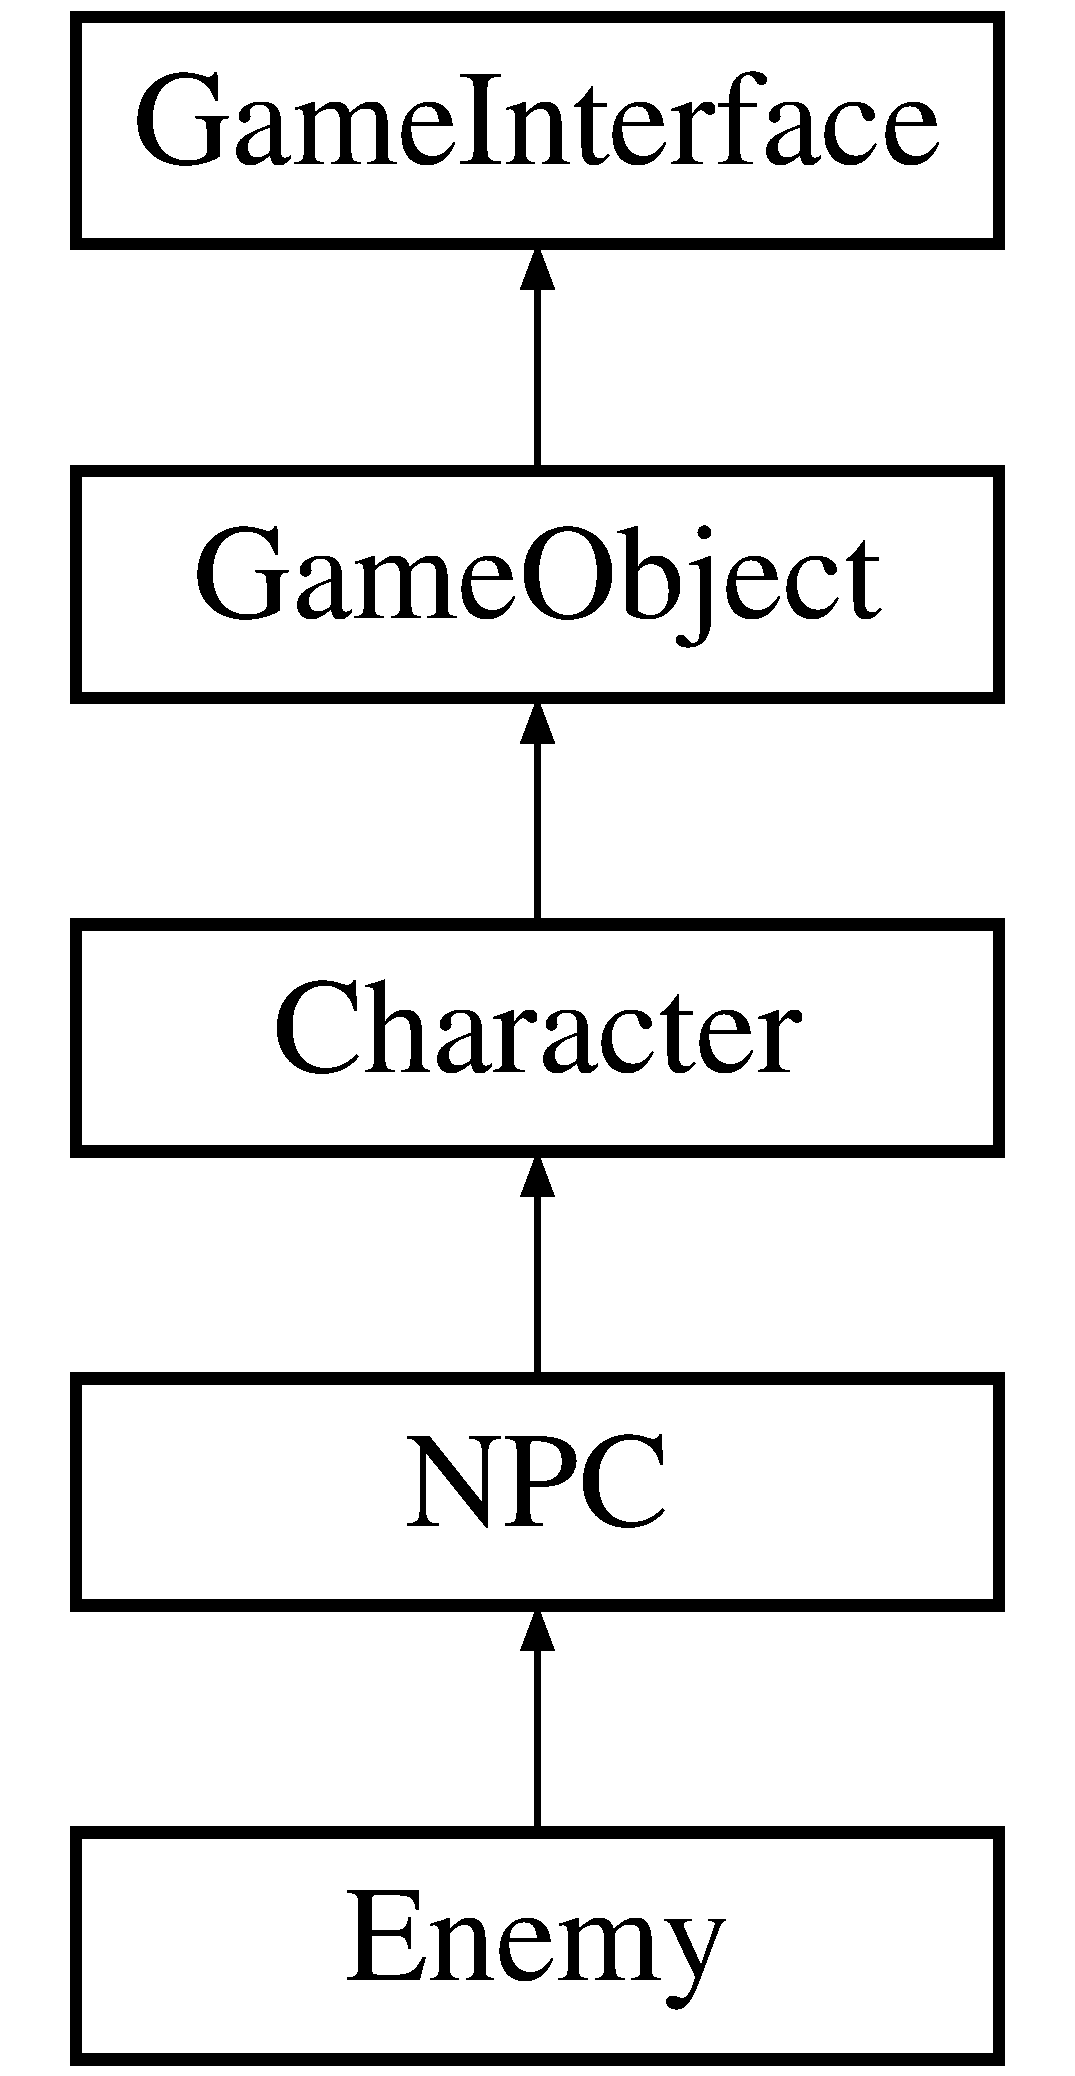
\includegraphics[height=5.000000cm]{class_n_p_c}
\end{center}
\end{figure}
\subsection*{Public Member Functions}
\begin{DoxyCompactItemize}
\item 
\hyperlink{class_n_p_c_a59b45912692304d555df9d6957046962}{N\-P\-C} ()
\item 
\hyperlink{class_n_p_c_a3416183550bea0c159cf154c41710fff}{N\-P\-C} (const \hyperlink{class_n_p_c}{N\-P\-C} \&other)
\item 
\hyperlink{class_n_p_c_a57565881c93d5b3839b8097ae16c38ae}{N\-P\-C} (\hyperlink{class_n_p_c}{N\-P\-C} \&\&other)
\item 
\hyperlink{class_n_p_c_a3afe2ba98d032697bdb09f9a08154614}{N\-P\-C} (const \hyperlink{struct_asset_file}{Asset\-File} \&image\-File, float \hyperlink{class_game_object_ac4637e122291be2421c851e2a87fb968}{size}, const \hyperlink{struct_position}{Position}$<$ float $>$ \&\hyperlink{class_game_object_a6858e668e7d2c5ded850b952aaacd905}{loc}, string \hyperlink{class_character_a2d423654566d1bf2160fef74bf04cc84}{name}, \hyperlink{_character_data_8h_acbff4d7298e294294555d39178aad448}{Do\-A} \hyperlink{class_character_ac83b99be690bb41b7fae53e9457838c6}{alive}, \hyperlink{_character_data_8h_aacbb008a93d24b04a8779bbdbd8880b5}{Character\-State} \hyperlink{class_character_ac20f1ebda238017ddc245ecdce827037}{state}, unsigned \hyperlink{class_character_ae8c0d82624dc3a171e2c3b42c699151e}{health}, unsigned \hyperlink{class_character_ae6a140637ffe5004179d90a0e04a411b}{damage}, bool monitor\-Velocity, \hyperlink{_character_data_8h_a0e5ce1612c1e71823c97a9cd734de339}{Reaction} \hyperlink{class_character_a579933775b2e4e97465bacb09c4e87f5}{reaction})
\item 
\hyperlink{class_n_p_c_a7b7d207fbbb2b27a1ca99cd7a533dce5}{N\-P\-C} (\hyperlink{class_fast_rand}{Fast\-Rand}$<$ int $>$ rand)
\item 
\hyperlink{class_n_p_c_a67c0caca129b56c82bb7ec8bce6be52b}{$\sim$\-N\-P\-C} ()
\item 
virtual \hyperlink{class_n_p_c}{N\-P\-C} \& \hyperlink{class_n_p_c_ae8d45c46413afc2d2ab08ff708c9d699}{operator=} (const \hyperlink{class_n_p_c}{N\-P\-C} \&rhs)
\item 
virtual \hyperlink{class_n_p_c}{N\-P\-C} \& \hyperlink{class_n_p_c_a19daaa71a87a22aa760db6ef639c3b53}{operator=} (\hyperlink{class_n_p_c}{N\-P\-C} \&\&rhs)
\item 
void \hyperlink{class_n_p_c_a73befe685fef40ab7f1ac954d932697d}{operator()} ()
\item 
void \hyperlink{class_n_p_c_a130d4f2fec85e20a54a060cbfcff64cc}{operator()} (\hyperlink{class_character}{Character} \&other)
\item 
void \hyperlink{class_n_p_c_ab590b71db4dd9dc21f6e2c183e9bd45c}{notify} ()
\item 
void \hyperlink{class_n_p_c_adfe9d4edaf5a31f3e3e9f727e86aa0b9}{pass\-Message} (\hyperlink{struct_message}{Message} $\ast$message, \hyperlink{class_character}{Character} \&recipient)
\item 
virtual void \hyperlink{class_n_p_c_ad85699c2a35f1f5f9d5a81a3d5df2153}{text\-Description} (ostream $\ast$write\-To) const 
\item 
void \hyperlink{class_n_p_c_a35234d189d4b9dee193b49f3d9272a0e}{attack} (\hyperlink{class_character}{Character} $\ast$enemy)
\item 
\hyperlink{_character_data_8h_a0e5ce1612c1e71823c97a9cd734de339}{Reaction} \hyperlink{class_n_p_c_ac595679b62ded86ebd5ed7e5d046ec2c}{get\-Reaction} ()
\end{DoxyCompactItemize}
\subsection*{Additional Inherited Members}


\subsection{Detailed Description}


Definition at line 19 of file N\-P\-C.\-h.



\subsection{Constructor \& Destructor Documentation}
\hypertarget{class_n_p_c_a59b45912692304d555df9d6957046962}{\index{N\-P\-C@{N\-P\-C}!N\-P\-C@{N\-P\-C}}
\index{N\-P\-C@{N\-P\-C}!NPC@{N\-P\-C}}
\subsubsection[{N\-P\-C}]{\setlength{\rightskip}{0pt plus 5cm}N\-P\-C\-::\-N\-P\-C (
\begin{DoxyParamCaption}
{}
\end{DoxyParamCaption}
)}}\label{class_n_p_c_a59b45912692304d555df9d6957046962}
Constructs a default \hyperlink{class_n_p_c}{N\-P\-C}. 

Definition at line 12 of file N\-P\-C.\-cpp.

\hypertarget{class_n_p_c_a3416183550bea0c159cf154c41710fff}{\index{N\-P\-C@{N\-P\-C}!N\-P\-C@{N\-P\-C}}
\index{N\-P\-C@{N\-P\-C}!NPC@{N\-P\-C}}
\subsubsection[{N\-P\-C}]{\setlength{\rightskip}{0pt plus 5cm}N\-P\-C\-::\-N\-P\-C (
\begin{DoxyParamCaption}
\item[{const {\bf N\-P\-C} \&}]{other}
\end{DoxyParamCaption}
)}}\label{class_n_p_c_a3416183550bea0c159cf154c41710fff}
Copy constructor for \hyperlink{class_n_p_c}{N\-P\-C}


\begin{DoxyParams}{Parameters}
{\em other} & The \hyperlink{class_n_p_c}{N\-P\-C} to be copied \\
\hline
\end{DoxyParams}


Definition at line 15 of file N\-P\-C.\-cpp.

\hypertarget{class_n_p_c_a57565881c93d5b3839b8097ae16c38ae}{\index{N\-P\-C@{N\-P\-C}!N\-P\-C@{N\-P\-C}}
\index{N\-P\-C@{N\-P\-C}!NPC@{N\-P\-C}}
\subsubsection[{N\-P\-C}]{\setlength{\rightskip}{0pt plus 5cm}N\-P\-C\-::\-N\-P\-C (
\begin{DoxyParamCaption}
\item[{{\bf N\-P\-C} \&\&}]{other}
\end{DoxyParamCaption}
)}}\label{class_n_p_c_a57565881c93d5b3839b8097ae16c38ae}
Move constructor for \hyperlink{class_n_p_c}{N\-P\-C}


\begin{DoxyParams}{Parameters}
{\em other} & The \hyperlink{class_n_p_c}{N\-P\-C} to be moved \\
\hline
\end{DoxyParams}


Definition at line 18 of file N\-P\-C.\-cpp.

\hypertarget{class_n_p_c_a3afe2ba98d032697bdb09f9a08154614}{\index{N\-P\-C@{N\-P\-C}!N\-P\-C@{N\-P\-C}}
\index{N\-P\-C@{N\-P\-C}!NPC@{N\-P\-C}}
\subsubsection[{N\-P\-C}]{\setlength{\rightskip}{0pt plus 5cm}N\-P\-C\-::\-N\-P\-C (
\begin{DoxyParamCaption}
\item[{const {\bf Asset\-File} \&}]{image\-File, }
\item[{float}]{size, }
\item[{const {\bf Position}$<$ float $>$ \&}]{loc, }
\item[{string}]{name, }
\item[{{\bf Do\-A}}]{alive, }
\item[{{\bf Character\-State}}]{state, }
\item[{unsigned}]{health, }
\item[{unsigned}]{damage, }
\item[{bool}]{monitor\-Velocity, }
\item[{{\bf Reaction}}]{reaction}
\end{DoxyParamCaption}
)}}\label{class_n_p_c_a3afe2ba98d032697bdb09f9a08154614}
Constructs an \hyperlink{class_n_p_c}{N\-P\-C} based on the arguments given


\begin{DoxyParams}{Parameters}
{\em name} & The name of this \hyperlink{class_n_p_c}{N\-P\-C} \\
\hline
{\em alive} & Whether this \hyperlink{class_n_p_c}{N\-P\-C} is dead or alive \\
\hline
{\em state} & The Character\-State of this \hyperlink{class_n_p_c}{N\-P\-C} \\
\hline
{\em health} & The \hyperlink{struct_health}{Health} of this \hyperlink{class_n_p_c}{N\-P\-C} \\
\hline
{\em damage} & The \hyperlink{struct_damage}{Damage} capability of this \hyperlink{class_n_p_c}{N\-P\-C} \\
\hline
{\em reaction} & The reaction of this \hyperlink{class_n_p_c}{N\-P\-C} to the player \\
\hline
\end{DoxyParams}


Definition at line 21 of file N\-P\-C.\-cpp.

\hypertarget{class_n_p_c_a7b7d207fbbb2b27a1ca99cd7a533dce5}{\index{N\-P\-C@{N\-P\-C}!N\-P\-C@{N\-P\-C}}
\index{N\-P\-C@{N\-P\-C}!NPC@{N\-P\-C}}
\subsubsection[{N\-P\-C}]{\setlength{\rightskip}{0pt plus 5cm}N\-P\-C\-::\-N\-P\-C (
\begin{DoxyParamCaption}
\item[{{\bf Fast\-Rand}$<$ int $>$}]{rand}
\end{DoxyParamCaption}
)}}\label{class_n_p_c_a7b7d207fbbb2b27a1ca99cd7a533dce5}
Constructs a randomized \hyperlink{class_n_p_c}{N\-P\-C}. The client has to option to simply leave the argument rand\-Seed as 0, in which case the constructor will generate its own random number.


\begin{DoxyParams}{Parameters}
{\em rand} & A seed to initialize the random number generator \\
\hline
\end{DoxyParams}


Definition at line 24 of file N\-P\-C.\-cpp.

\hypertarget{class_n_p_c_a67c0caca129b56c82bb7ec8bce6be52b}{\index{N\-P\-C@{N\-P\-C}!$\sim$\-N\-P\-C@{$\sim$\-N\-P\-C}}
\index{$\sim$\-N\-P\-C@{$\sim$\-N\-P\-C}!NPC@{N\-P\-C}}
\subsubsection[{$\sim$\-N\-P\-C}]{\setlength{\rightskip}{0pt plus 5cm}N\-P\-C\-::$\sim$\-N\-P\-C (
\begin{DoxyParamCaption}
{}
\end{DoxyParamCaption}
)}}\label{class_n_p_c_a67c0caca129b56c82bb7ec8bce6be52b}
Destructor for \hyperlink{class_n_p_c}{N\-P\-C} 

Definition at line 31 of file N\-P\-C.\-cpp.



\subsection{Member Function Documentation}
\hypertarget{class_n_p_c_a35234d189d4b9dee193b49f3d9272a0e}{\index{N\-P\-C@{N\-P\-C}!attack@{attack}}
\index{attack@{attack}!NPC@{N\-P\-C}}
\subsubsection[{attack}]{\setlength{\rightskip}{0pt plus 5cm}void N\-P\-C\-::attack (
\begin{DoxyParamCaption}
\item[{{\bf Character} $\ast$}]{enemy}
\end{DoxyParamCaption}
)\hspace{0.3cm}{\ttfamily [virtual]}}}\label{class_n_p_c_a35234d189d4b9dee193b49f3d9272a0e}
Attacks a hostile \hyperlink{class_n_p_c}{N\-P\-C}


\begin{DoxyParams}{Parameters}
{\em enemy} & The enemy to attack \\
\hline
\end{DoxyParams}


Reimplemented from \hyperlink{class_character_a7be3b65a2bc5facbb39ee208f5898560}{Character}.



Definition at line 74 of file N\-P\-C.\-cpp.

\hypertarget{class_n_p_c_ac595679b62ded86ebd5ed7e5d046ec2c}{\index{N\-P\-C@{N\-P\-C}!get\-Reaction@{get\-Reaction}}
\index{get\-Reaction@{get\-Reaction}!NPC@{N\-P\-C}}
\subsubsection[{get\-Reaction}]{\setlength{\rightskip}{0pt plus 5cm}{\bf Reaction} N\-P\-C\-::get\-Reaction (
\begin{DoxyParamCaption}
{}
\end{DoxyParamCaption}
)\hspace{0.3cm}{\ttfamily [inline]}}}\label{class_n_p_c_ac595679b62ded86ebd5ed7e5d046ec2c}
Returns this \hyperlink{class_n_p_c}{N\-P\-C}'s reaction (attitude) toward the player 

Definition at line 141 of file N\-P\-C.\-h.

\hypertarget{class_n_p_c_ab590b71db4dd9dc21f6e2c183e9bd45c}{\index{N\-P\-C@{N\-P\-C}!notify@{notify}}
\index{notify@{notify}!NPC@{N\-P\-C}}
\subsubsection[{notify}]{\setlength{\rightskip}{0pt plus 5cm}void N\-P\-C\-::notify (
\begin{DoxyParamCaption}
{}
\end{DoxyParamCaption}
)\hspace{0.3cm}{\ttfamily [virtual]}}}\label{class_n_p_c_ab590b71db4dd9dc21f6e2c183e9bd45c}
Another class with a reference to this \hyperlink{class_n_p_c}{N\-P\-C} can call this to have the \hyperlink{class_n_p_c}{N\-P\-C} perform some function, as yet undecided. T\-B\-I. 

Reimplemented from \hyperlink{class_character_a457dab4f04550716888425da681b9f1f}{Character}.



Definition at line 59 of file N\-P\-C.\-cpp.

\hypertarget{class_n_p_c_a73befe685fef40ab7f1ac954d932697d}{\index{N\-P\-C@{N\-P\-C}!operator()@{operator()}}
\index{operator()@{operator()}!NPC@{N\-P\-C}}
\subsubsection[{operator()}]{\setlength{\rightskip}{0pt plus 5cm}void N\-P\-C\-::operator() (
\begin{DoxyParamCaption}
{}
\end{DoxyParamCaption}
)\hspace{0.3cm}{\ttfamily [virtual]}}}\label{class_n_p_c_a73befe685fef40ab7f1ac954d932697d}
Overloads operator() for \hyperlink{class_n_p_c}{N\-P\-C}. Possibly will be used to call \hyperlink{class_n_p_c_ab590b71db4dd9dc21f6e2c183e9bd45c}{notify()}. T\-B\-D. 

Reimplemented from \hyperlink{class_character_a3c4dfc59865fe39251070cd0b92d34ac}{Character}.



Definition at line 51 of file N\-P\-C.\-cpp.

\hypertarget{class_n_p_c_a130d4f2fec85e20a54a060cbfcff64cc}{\index{N\-P\-C@{N\-P\-C}!operator()@{operator()}}
\index{operator()@{operator()}!NPC@{N\-P\-C}}
\subsubsection[{operator()}]{\setlength{\rightskip}{0pt plus 5cm}void N\-P\-C\-::operator() (
\begin{DoxyParamCaption}
\item[{{\bf Character} \&}]{other}
\end{DoxyParamCaption}
)}}\label{class_n_p_c_a130d4f2fec85e20a54a060cbfcff64cc}
Overloads the overload of operator(). The actual implementation and uses for this are still undecided.


\begin{DoxyParams}{Parameters}
{\em other} & A reference to another \hyperlink{class_n_p_c}{N\-P\-C} \\
\hline
\end{DoxyParams}


Definition at line 55 of file N\-P\-C.\-cpp.

\hypertarget{class_n_p_c_ae8d45c46413afc2d2ab08ff708c9d699}{\index{N\-P\-C@{N\-P\-C}!operator=@{operator=}}
\index{operator=@{operator=}!NPC@{N\-P\-C}}
\subsubsection[{operator=}]{\setlength{\rightskip}{0pt plus 5cm}{\bf N\-P\-C} \& N\-P\-C\-::operator= (
\begin{DoxyParamCaption}
\item[{const {\bf N\-P\-C} \&}]{rhs}
\end{DoxyParamCaption}
)\hspace{0.3cm}{\ttfamily [virtual]}}}\label{class_n_p_c_ae8d45c46413afc2d2ab08ff708c9d699}
Assignment operator overload (copy)


\begin{DoxyParams}{Parameters}
{\em rhs} & The right hand side argument (which will be copied) \\
\hline
\end{DoxyParams}


Definition at line 36 of file N\-P\-C.\-cpp.

\hypertarget{class_n_p_c_a19daaa71a87a22aa760db6ef639c3b53}{\index{N\-P\-C@{N\-P\-C}!operator=@{operator=}}
\index{operator=@{operator=}!NPC@{N\-P\-C}}
\subsubsection[{operator=}]{\setlength{\rightskip}{0pt plus 5cm}{\bf N\-P\-C} \& N\-P\-C\-::operator= (
\begin{DoxyParamCaption}
\item[{{\bf N\-P\-C} \&\&}]{rhs}
\end{DoxyParamCaption}
)\hspace{0.3cm}{\ttfamily [virtual]}}}\label{class_n_p_c_a19daaa71a87a22aa760db6ef639c3b53}
Assignment operator overload (move)


\begin{DoxyParams}{Parameters}
{\em rhs} & The right hand side argument (which will be moved) \\
\hline
\end{DoxyParams}


Definition at line 43 of file N\-P\-C.\-cpp.

\hypertarget{class_n_p_c_adfe9d4edaf5a31f3e3e9f727e86aa0b9}{\index{N\-P\-C@{N\-P\-C}!pass\-Message@{pass\-Message}}
\index{pass\-Message@{pass\-Message}!NPC@{N\-P\-C}}
\subsubsection[{pass\-Message}]{\setlength{\rightskip}{0pt plus 5cm}void N\-P\-C\-::pass\-Message (
\begin{DoxyParamCaption}
\item[{{\bf Message} $\ast$}]{message, }
\item[{{\bf Character} \&}]{recipient}
\end{DoxyParamCaption}
)}}\label{class_n_p_c_adfe9d4edaf5a31f3e3e9f727e86aa0b9}
A \hyperlink{class_n_p_c}{N\-P\-C} can use this function to pass messages to another.


\begin{DoxyParams}{Parameters}
{\em message} & The \hyperlink{struct_message}{Message} sent by this \\
\hline
{\em recipient} & The object receiving the \hyperlink{struct_message}{Message} \\
\hline
\end{DoxyParams}


Definition at line 63 of file N\-P\-C.\-cpp.

\hypertarget{class_n_p_c_ad85699c2a35f1f5f9d5a81a3d5df2153}{\index{N\-P\-C@{N\-P\-C}!text\-Description@{text\-Description}}
\index{text\-Description@{text\-Description}!NPC@{N\-P\-C}}
\subsubsection[{text\-Description}]{\setlength{\rightskip}{0pt plus 5cm}void N\-P\-C\-::text\-Description (
\begin{DoxyParamCaption}
\item[{ostream $\ast$}]{write\-To}
\end{DoxyParamCaption}
) const\hspace{0.3cm}{\ttfamily [virtual]}}}\label{class_n_p_c_ad85699c2a35f1f5f9d5a81a3d5df2153}
Writes a formatted text description of this \hyperlink{class_n_p_c}{N\-P\-C} into the desired output stream 

Reimplemented from \hyperlink{class_character_a2ab1090f959f0c66b098e0463d4c1bdd}{Character}.



Definition at line 67 of file N\-P\-C.\-cpp.



The documentation for this class was generated from the following files\-:\begin{DoxyCompactItemize}
\item 
/\-Volumes/\-O\-S X H\-D\-D/\-Users/\-Adam/\-Developer/\-Sprite\-Fight/\-World/\hyperlink{_n_p_c_8h}{N\-P\-C.\-h}\item 
/\-Volumes/\-O\-S X H\-D\-D/\-Users/\-Adam/\-Developer/\-Sprite\-Fight/\-World/\hyperlink{_n_p_c_8cpp}{N\-P\-C.\-cpp}\end{DoxyCompactItemize}

\hypertarget{struct_output_data}{\section{Output\-Data$<$ P\-O\-S\-U\-T\-Y\-P\-E, S\-I\-Z\-E\-U\-T\-Y\-P\-E $>$ Struct Template Reference}
\label{struct_output_data}\index{Output\-Data$<$ P\-O\-S\-U\-T\-Y\-P\-E, S\-I\-Z\-E\-U\-T\-Y\-P\-E $>$@{Output\-Data$<$ P\-O\-S\-U\-T\-Y\-P\-E, S\-I\-Z\-E\-U\-T\-Y\-P\-E $>$}}
}


{\ttfamily \#include $<$Game\-State.\-hpp$>$}

Inheritance diagram for Output\-Data$<$ P\-O\-S\-U\-T\-Y\-P\-E, S\-I\-Z\-E\-U\-T\-Y\-P\-E $>$\-:\begin{figure}[H]
\begin{center}
\leavevmode
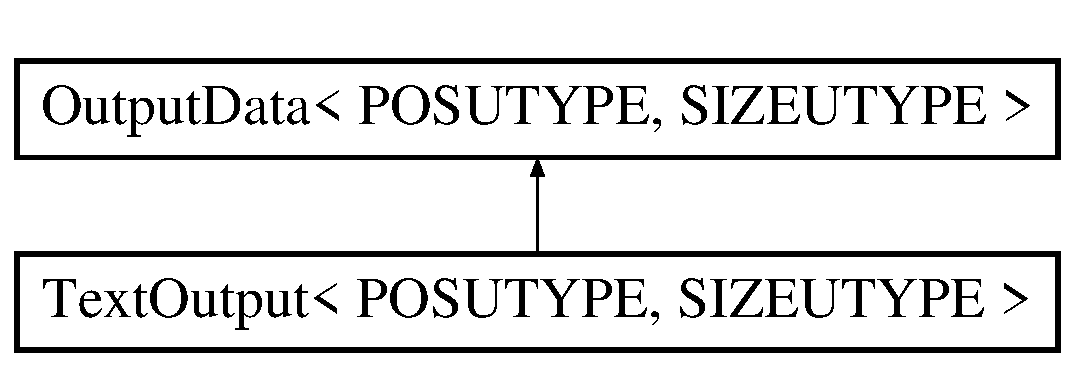
\includegraphics[height=2.000000cm]{struct_output_data}
\end{center}
\end{figure}
\subsection*{Public Member Functions}
\begin{DoxyCompactItemize}
\item 
\hyperlink{struct_output_data_a25dd66307e7a48c4bc0d25e0016238fb}{Output\-Data} ()
\item 
\hyperlink{struct_output_data_a5f9343b49b12d6eaebcf0a4f97091a4d}{Output\-Data} (\hyperlink{struct_position}{Position}$<$ P\-O\-S\-U\-T\-Y\-P\-E $>$ $\ast$pos, const float size\-Modifier, \hyperlink{_output_data_8hpp_aa80fe4e9a559009407475c9587214b48}{Position\-Type} type)
\item 
\hyperlink{struct_output_data_a4d1b3008b1fb7dbb4cf9de8e89414f78}{Output\-Data} (const \hyperlink{struct_asset_file}{Asset\-File} \&file, const \hyperlink{struct_position}{Position}$<$ P\-O\-S\-U\-T\-Y\-P\-E $>$ $\ast$pos, const float size\-Modifier, \hyperlink{_output_data_8hpp_aa80fe4e9a559009407475c9587214b48}{Position\-Type} type)
\item 
\hyperlink{struct_output_data_a31419d6be305d81146da03acf50af852}{Output\-Data} (\hyperlink{class_fast_rand}{Fast\-Rand}$<$ int $>$ \&randm, const \hyperlink{struct_position}{Position}$<$ P\-O\-S\-U\-T\-Y\-P\-E $>$ $\ast$pos, const float size\-Modifier, \hyperlink{_output_data_8hpp_aa80fe4e9a559009407475c9587214b48}{Position\-Type} type)
\item 
\hyperlink{struct_output_data_a40e2554a288f7e546593eb866cdd1baf}{Output\-Data} (const \hyperlink{struct_output_data}{Output\-Data} \&other)
\item 
\hyperlink{struct_output_data_ab73d0b798428ee36881b61250bd152ac}{Output\-Data} (\hyperlink{struct_output_data}{Output\-Data} \&\&other)
\item 
\hyperlink{struct_output_data_ab9a358e297a61ab8c134376ddddf1c13}{$\sim$\-Output\-Data} ()
\item 
\hyperlink{struct_output_data}{Output\-Data} \& \hyperlink{struct_output_data_ad95e5bfff9550c7290c966887e50dd6d}{operator=} (const \hyperlink{struct_output_data}{Output\-Data} \&rhs)=delete
\item 
\hyperlink{struct_output_data}{Output\-Data} \& \hyperlink{struct_output_data_acaaf3bcc5ca785c4b96518215d7ecb82}{operator=} (\hyperlink{struct_output_data}{Output\-Data} \&\&rhs)=delete
\item 
void \hyperlink{struct_output_data_ac9c208239b472eea752f3605b155c713}{reinitialize\-Members} (const \hyperlink{struct_asset_file}{Asset\-File} \&file, const \hyperlink{struct_position}{Position}$<$ P\-O\-S\-U\-T\-Y\-P\-E $>$ $\ast$pos, const float size\-Modifier, \hyperlink{_output_data_8hpp_aa80fe4e9a559009407475c9587214b48}{Position\-Type} type)
\item 
void \hyperlink{struct_output_data_a6cdf1d5f73c6ac03a2b46ce65d01c870}{reinitialize\-Members} (\hyperlink{class_fast_rand}{Fast\-Rand}$<$ int $>$ \&randm, const \hyperlink{struct_position}{Position}$<$ P\-O\-S\-U\-T\-Y\-P\-E $>$ $\ast$pos, const float size\-Modifier, \hyperlink{_output_data_8hpp_aa80fe4e9a559009407475c9587214b48}{Position\-Type} type)
\item 
bool \hyperlink{struct_output_data_a2b19b9cd0df099c3f923f9c5f1ef28d9}{check\-If\-Updated} ()
\begin{DoxyCompactList}\small\item\em Check whether this \hyperlink{struct_output_data}{Output\-Data} has changed since the last time it was rendered. \end{DoxyCompactList}\item 
void \hyperlink{struct_output_data_a43ba11266165462930555fce963d20d9}{set\-Asset\-File} (string image\-File\-Name)
\item 
const \hyperlink{struct_asset_file}{Asset\-File} $\ast$ \hyperlink{struct_output_data_aa098f57388970d839d6eb55b333b1feb}{get\-Asset\-File} () const 
\item 
void \hyperlink{struct_output_data_a486ecf698661a03fd0740c83cd5ebe39}{set\-Texture} (\hyperlink{_default_config_8h_a9ca20d8445e7d830c262f5ec4bb5d1bf}{Texture} $\ast$\hyperlink{struct_output_data_af592125b9117db60d387049a7631c763}{texture})
\item 
\hyperlink{_default_config_8h_a9ca20d8445e7d830c262f5ec4bb5d1bf}{Texture} $\ast$ \hyperlink{struct_output_data_abae817843824525377ff87dff98825f1}{get\-Texture} () const 
\item 
const \hyperlink{struct_position}{Position}$<$ P\-O\-S\-U\-T\-Y\-P\-E $>$ \hyperlink{struct_output_data_acafb00ba35ee770e08f37de9080430a1}{get\-Position} () const 
\item 
const \hyperlink{struct_position}{Position}$<$ P\-O\-S\-U\-T\-Y\-P\-E $>$ $\ast$ \hyperlink{struct_output_data_a472127a33bcf404202ce9481a5ac8c4b}{get\-Position\-\_\-raw} () const 
\item 
\hyperlink{_output_data_8hpp_aa80fe4e9a559009407475c9587214b48}{Position\-Type} \hyperlink{struct_output_data_ae5a31a3636b1ebcebb70da1d8e2b5111}{get\-Position\-Type} () const 
\item 
const \hyperlink{struct_size}{Size}$<$ S\-I\-Z\-E\-U\-T\-Y\-P\-E $>$ \hyperlink{struct_output_data_a3bffb05a3714e4c93adb33bce30cc86d}{get\-Size} () const 
\item 
void \hyperlink{struct_output_data_a286c4b1e5d7abf94af4d9f5eb454100e}{set\-Visibility} (bool \hyperlink{struct_output_data_ab1d5abc732db0f826a01afbea44ada34}{visible})
\item 
bool \hyperlink{struct_output_data_aeaa3ed34010dfb0726897b9722a779fa}{is\-Visible} () const 
\end{DoxyCompactItemize}
\subsection*{Static Public Member Functions}
\begin{DoxyCompactItemize}
\item 
static vector$<$ \hyperlink{struct_output_data}{Output\-Data} $\ast$ $>$ $\ast$ \hyperlink{struct_output_data_ad67cc040f7336e2c4de57bd852bf3116}{get\-Output\-Data} ()
\item 
static void \hyperlink{struct_output_data_a1d35bb8a17ff06cd584d879bf30b2445}{update\-All} ()
\end{DoxyCompactItemize}
\subsection*{Protected Member Functions}
\begin{DoxyCompactItemize}
\item 
virtual void \hyperlink{struct_output_data_a7bca309627422d32bd485356394a4ed8}{complete\-Initialization} ()
\begin{DoxyCompactList}\small\item\em Does the remaining initialization that could not be done in the constructor (because it does not know with certainty that it is on the main thread) \end{DoxyCompactList}\item 
virtual void \hyperlink{struct_output_data_aed0e4b81a7c981a7f2a0d6128ee69eb7}{update} ()
\end{DoxyCompactItemize}
\subsection*{Protected Attributes}
\begin{DoxyCompactItemize}
\item 
bool \hyperlink{struct_output_data_a4b90649aee88b935b5ebf38dee4aff7b}{init\-Flag} = true
\item 
bool \hyperlink{struct_output_data_ab1d5abc732db0f826a01afbea44ada34}{visible} = true
\begin{DoxyCompactList}\small\item\em Indicates whether the \hyperlink{struct_output_data}{Output\-Data} has been recently updated. For every member that changes, it's corresponding boolean within update\-Flags should be set true. Don't refer to this directly, instead call \hyperlink{struct_output_data_a2b19b9cd0df099c3f923f9c5f1ef28d9}{check\-If\-Updated()} \end{DoxyCompactList}\item 
bool \hyperlink{struct_output_data_a0f15b2dc64531dfd8dd0925840c4758e}{visibility\-\_\-was\-\_\-updated} = false
\item 
\hyperlink{_output_data_8hpp_aa80fe4e9a559009407475c9587214b48}{Position\-Type} \hyperlink{struct_output_data_a344be69157cfd43c9ace4158b0e58b6b}{position\-Type}
\item 
\hyperlink{struct_asset_file}{Asset\-File} \hyperlink{struct_output_data_aada926eef9e2b2b654caa32de712ef1b}{texture\-Image\-File}
\item 
\hyperlink{_default_config_8h_a9ca20d8445e7d830c262f5ec4bb5d1bf}{Texture} $\ast$ \hyperlink{struct_output_data_af592125b9117db60d387049a7631c763}{texture}
\begin{DoxyCompactList}\small\item\em A texture. \end{DoxyCompactList}\item 
bool \hyperlink{struct_output_data_aa35a2457b23d1a6843ec49c2f6a4b29a}{texture\-\_\-was\-\_\-updated}
\item 
const \hyperlink{struct_position}{Position}$<$ P\-O\-S\-U\-T\-Y\-P\-E $>$ $\ast$ \hyperlink{struct_output_data_a7494156691e440a9a6f2c808321b0cd5}{position}
\begin{DoxyCompactList}\small\item\em A pointer to a \hyperlink{struct_position}{Position} object, which in most cases is owned by the class that owns this \hyperlink{struct_output_data}{Output\-Data} object. \end{DoxyCompactList}\item 
\hyperlink{struct_size}{Size}$<$ S\-I\-Z\-E\-U\-T\-Y\-P\-E $>$ \hyperlink{struct_output_data_aa0cfd47e41dd6e32a43b10cecdcbeb2b}{size}
\begin{DoxyCompactList}\small\item\em A \hyperlink{struct_size}{Size} object, which unlike position is not a pointer and is owned by the \hyperlink{struct_output_data}{Output\-Data} object. \end{DoxyCompactList}\item 
\hyperlink{struct_position}{Position}$<$ P\-O\-S\-U\-T\-Y\-P\-E $>$ \hyperlink{struct_output_data_a21ec70c5ab2418a33e9c6293dd9b588d}{position\-\_\-last\-Recorded\-Value}
\begin{DoxyCompactList}\small\item\em A copy of position from the last time this \hyperlink{struct_output_data}{Output\-Data} was updated. \end{DoxyCompactList}\item 
\hyperlink{struct_size}{Size}$<$ S\-I\-Z\-E\-U\-T\-Y\-P\-E $>$ \hyperlink{struct_output_data_a3007edb5d6739619f9e6b3f8ae8e5be1}{size\-\_\-last\-Recorded\-Value}
\begin{DoxyCompactList}\small\item\em A copy of size from the last time this \hyperlink{struct_output_data}{Output\-Data} was updated. \end{DoxyCompactList}\item 
vector$<$ bool $\ast$ $>$ \hyperlink{struct_output_data_a490cb05683b60fb16e696652b0c040d6}{update\-Flags} = \{ \& \hyperlink{struct_output_data_a0f15b2dc64531dfd8dd0925840c4758e}{visibility\-\_\-was\-\_\-updated}, \& \hyperlink{struct_output_data_aa35a2457b23d1a6843ec49c2f6a4b29a}{texture\-\_\-was\-\_\-updated} \}
\end{DoxyCompactItemize}
\subsection*{Static Protected Attributes}
\begin{DoxyCompactItemize}
\item 
static vector$<$ \hyperlink{struct_output_data}{Output\-Data} $\ast$ $>$ \hyperlink{struct_output_data_ad515b68d5527925323d98113f08b5d8f}{all\-Output\-Data}
\end{DoxyCompactItemize}


\subsection{Detailed Description}
\subsubsection*{template$<$typename P\-O\-S\-U\-T\-Y\-P\-E, typename S\-I\-Z\-E\-U\-T\-Y\-P\-E$>$struct Output\-Data$<$ P\-O\-S\-U\-T\-Y\-P\-E, S\-I\-Z\-E\-U\-T\-Y\-P\-E $>$}



Definition at line 40 of file Game\-State.\-hpp.



\subsection{Constructor \& Destructor Documentation}
\hypertarget{struct_output_data_a25dd66307e7a48c4bc0d25e0016238fb}{\index{Output\-Data@{Output\-Data}!Output\-Data@{Output\-Data}}
\index{Output\-Data@{Output\-Data}!OutputData@{Output\-Data}}
\subsubsection[{Output\-Data}]{\setlength{\rightskip}{0pt plus 5cm}template$<$typename P\-O\-S\-U\-T\-Y\-P\-E, typename S\-I\-Z\-E\-U\-T\-Y\-P\-E$>$ {\bf Output\-Data}$<$ P\-O\-S\-U\-T\-Y\-P\-E, S\-I\-Z\-E\-U\-T\-Y\-P\-E $>$\-::{\bf Output\-Data} (
\begin{DoxyParamCaption}
{}
\end{DoxyParamCaption}
)\hspace{0.3cm}{\ttfamily [inline]}}}\label{struct_output_data_a25dd66307e7a48c4bc0d25e0016238fb}


Definition at line 118 of file Output\-Data.\-hpp.

\hypertarget{struct_output_data_a5f9343b49b12d6eaebcf0a4f97091a4d}{\index{Output\-Data@{Output\-Data}!Output\-Data@{Output\-Data}}
\index{Output\-Data@{Output\-Data}!OutputData@{Output\-Data}}
\subsubsection[{Output\-Data}]{\setlength{\rightskip}{0pt plus 5cm}template$<$typename P\-O\-S\-U\-T\-Y\-P\-E, typename S\-I\-Z\-E\-U\-T\-Y\-P\-E$>$ {\bf Output\-Data}$<$ P\-O\-S\-U\-T\-Y\-P\-E, S\-I\-Z\-E\-U\-T\-Y\-P\-E $>$\-::{\bf Output\-Data} (
\begin{DoxyParamCaption}
\item[{{\bf Position}$<$ P\-O\-S\-U\-T\-Y\-P\-E $>$ $\ast$}]{pos, }
\item[{const float}]{size\-Modifier, }
\item[{{\bf Position\-Type}}]{type}
\end{DoxyParamCaption}
)\hspace{0.3cm}{\ttfamily [inline]}}}\label{struct_output_data_a5f9343b49b12d6eaebcf0a4f97091a4d}


Definition at line 128 of file Output\-Data.\-hpp.

\hypertarget{struct_output_data_a4d1b3008b1fb7dbb4cf9de8e89414f78}{\index{Output\-Data@{Output\-Data}!Output\-Data@{Output\-Data}}
\index{Output\-Data@{Output\-Data}!OutputData@{Output\-Data}}
\subsubsection[{Output\-Data}]{\setlength{\rightskip}{0pt plus 5cm}template$<$typename P\-O\-S\-U\-T\-Y\-P\-E, typename S\-I\-Z\-E\-U\-T\-Y\-P\-E$>$ {\bf Output\-Data}$<$ P\-O\-S\-U\-T\-Y\-P\-E, S\-I\-Z\-E\-U\-T\-Y\-P\-E $>$\-::{\bf Output\-Data} (
\begin{DoxyParamCaption}
\item[{const {\bf Asset\-File} \&}]{file, }
\item[{const {\bf Position}$<$ P\-O\-S\-U\-T\-Y\-P\-E $>$ $\ast$}]{pos, }
\item[{const float}]{size\-Modifier, }
\item[{{\bf Position\-Type}}]{type}
\end{DoxyParamCaption}
)\hspace{0.3cm}{\ttfamily [inline]}}}\label{struct_output_data_a4d1b3008b1fb7dbb4cf9de8e89414f78}


Definition at line 140 of file Output\-Data.\-hpp.

\hypertarget{struct_output_data_a31419d6be305d81146da03acf50af852}{\index{Output\-Data@{Output\-Data}!Output\-Data@{Output\-Data}}
\index{Output\-Data@{Output\-Data}!OutputData@{Output\-Data}}
\subsubsection[{Output\-Data}]{\setlength{\rightskip}{0pt plus 5cm}template$<$typename P\-O\-S\-U\-T\-Y\-P\-E, typename S\-I\-Z\-E\-U\-T\-Y\-P\-E$>$ {\bf Output\-Data}$<$ P\-O\-S\-U\-T\-Y\-P\-E, S\-I\-Z\-E\-U\-T\-Y\-P\-E $>$\-::{\bf Output\-Data} (
\begin{DoxyParamCaption}
\item[{{\bf Fast\-Rand}$<$ int $>$ \&}]{randm, }
\item[{const {\bf Position}$<$ P\-O\-S\-U\-T\-Y\-P\-E $>$ $\ast$}]{pos, }
\item[{const float}]{size\-Modifier, }
\item[{{\bf Position\-Type}}]{type}
\end{DoxyParamCaption}
)\hspace{0.3cm}{\ttfamily [inline]}}}\label{struct_output_data_a31419d6be305d81146da03acf50af852}


Definition at line 152 of file Output\-Data.\-hpp.

\hypertarget{struct_output_data_a40e2554a288f7e546593eb866cdd1baf}{\index{Output\-Data@{Output\-Data}!Output\-Data@{Output\-Data}}
\index{Output\-Data@{Output\-Data}!OutputData@{Output\-Data}}
\subsubsection[{Output\-Data}]{\setlength{\rightskip}{0pt plus 5cm}template$<$typename P\-O\-S\-U\-T\-Y\-P\-E, typename S\-I\-Z\-E\-U\-T\-Y\-P\-E$>$ {\bf Output\-Data}$<$ P\-O\-S\-U\-T\-Y\-P\-E, S\-I\-Z\-E\-U\-T\-Y\-P\-E $>$\-::{\bf Output\-Data} (
\begin{DoxyParamCaption}
\item[{const {\bf Output\-Data}$<$ P\-O\-S\-U\-T\-Y\-P\-E, S\-I\-Z\-E\-U\-T\-Y\-P\-E $>$ \&}]{other}
\end{DoxyParamCaption}
)\hspace{0.3cm}{\ttfamily [inline]}}}\label{struct_output_data_a40e2554a288f7e546593eb866cdd1baf}


Definition at line 164 of file Output\-Data.\-hpp.

\hypertarget{struct_output_data_ab73d0b798428ee36881b61250bd152ac}{\index{Output\-Data@{Output\-Data}!Output\-Data@{Output\-Data}}
\index{Output\-Data@{Output\-Data}!OutputData@{Output\-Data}}
\subsubsection[{Output\-Data}]{\setlength{\rightskip}{0pt plus 5cm}template$<$typename P\-O\-S\-U\-T\-Y\-P\-E, typename S\-I\-Z\-E\-U\-T\-Y\-P\-E$>$ {\bf Output\-Data}$<$ P\-O\-S\-U\-T\-Y\-P\-E, S\-I\-Z\-E\-U\-T\-Y\-P\-E $>$\-::{\bf Output\-Data} (
\begin{DoxyParamCaption}
\item[{{\bf Output\-Data}$<$ P\-O\-S\-U\-T\-Y\-P\-E, S\-I\-Z\-E\-U\-T\-Y\-P\-E $>$ \&\&}]{other}
\end{DoxyParamCaption}
)\hspace{0.3cm}{\ttfamily [inline]}}}\label{struct_output_data_ab73d0b798428ee36881b61250bd152ac}


Definition at line 178 of file Output\-Data.\-hpp.

\hypertarget{struct_output_data_ab9a358e297a61ab8c134376ddddf1c13}{\index{Output\-Data@{Output\-Data}!$\sim$\-Output\-Data@{$\sim$\-Output\-Data}}
\index{$\sim$\-Output\-Data@{$\sim$\-Output\-Data}!OutputData@{Output\-Data}}
\subsubsection[{$\sim$\-Output\-Data}]{\setlength{\rightskip}{0pt plus 5cm}template$<$typename P\-O\-S\-U\-T\-Y\-P\-E, typename S\-I\-Z\-E\-U\-T\-Y\-P\-E$>$ {\bf Output\-Data}$<$ P\-O\-S\-U\-T\-Y\-P\-E, S\-I\-Z\-E\-U\-T\-Y\-P\-E $>$\-::$\sim${\bf Output\-Data} (
\begin{DoxyParamCaption}
{}
\end{DoxyParamCaption}
)\hspace{0.3cm}{\ttfamily [inline]}}}\label{struct_output_data_ab9a358e297a61ab8c134376ddddf1c13}


Definition at line 196 of file Output\-Data.\-hpp.



\subsection{Member Function Documentation}
\hypertarget{struct_output_data_a2b19b9cd0df099c3f923f9c5f1ef28d9}{\index{Output\-Data@{Output\-Data}!check\-If\-Updated@{check\-If\-Updated}}
\index{check\-If\-Updated@{check\-If\-Updated}!OutputData@{Output\-Data}}
\subsubsection[{check\-If\-Updated}]{\setlength{\rightskip}{0pt plus 5cm}template$<$typename P\-O\-S\-U\-T\-Y\-P\-E , typename S\-I\-Z\-E\-U\-T\-Y\-P\-E $>$ bool {\bf Output\-Data}$<$ P\-O\-S\-U\-T\-Y\-P\-E, S\-I\-Z\-E\-U\-T\-Y\-P\-E $>$\-::check\-If\-Updated (
\begin{DoxyParamCaption}
{}
\end{DoxyParamCaption}
)}}\label{struct_output_data_a2b19b9cd0df099c3f923f9c5f1ef28d9}


Check whether this \hyperlink{struct_output_data}{Output\-Data} has changed since the last time it was rendered. 

\begin{DoxyReturn}{Returns}
Whether this \hyperlink{struct_output_data}{Output\-Data} has changed since the last time it was rendered 
\end{DoxyReturn}


Definition at line 411 of file Output\-Data.\-hpp.

\hypertarget{struct_output_data_a7bca309627422d32bd485356394a4ed8}{\index{Output\-Data@{Output\-Data}!complete\-Initialization@{complete\-Initialization}}
\index{complete\-Initialization@{complete\-Initialization}!OutputData@{Output\-Data}}
\subsubsection[{complete\-Initialization}]{\setlength{\rightskip}{0pt plus 5cm}template$<$typename P\-O\-S\-U\-T\-Y\-P\-E , typename S\-I\-Z\-E\-U\-T\-Y\-P\-E $>$ void {\bf Output\-Data}$<$ P\-O\-S\-U\-T\-Y\-P\-E, S\-I\-Z\-E\-U\-T\-Y\-P\-E $>$\-::complete\-Initialization (
\begin{DoxyParamCaption}
{}
\end{DoxyParamCaption}
)\hspace{0.3cm}{\ttfamily [protected]}, {\ttfamily [virtual]}}}\label{struct_output_data_a7bca309627422d32bd485356394a4ed8}


Does the remaining initialization that could not be done in the constructor (because it does not know with certainty that it is on the main thread) 

\begin{DoxyNote}{Note}
Can O\-N\-L\-Y be run on the main thread 
\end{DoxyNote}


Reimplemented in \hyperlink{class_text_output_a77b70d1145a189362996cd6b308e7dde}{Text\-Output$<$ P\-O\-S\-U\-T\-Y\-P\-E, S\-I\-Z\-E\-U\-T\-Y\-P\-E $>$}.



Definition at line 357 of file Output\-Data.\-hpp.

\hypertarget{struct_output_data_aa098f57388970d839d6eb55b333b1feb}{\index{Output\-Data@{Output\-Data}!get\-Asset\-File@{get\-Asset\-File}}
\index{get\-Asset\-File@{get\-Asset\-File}!OutputData@{Output\-Data}}
\subsubsection[{get\-Asset\-File}]{\setlength{\rightskip}{0pt plus 5cm}template$<$typename P\-O\-S\-U\-T\-Y\-P\-E, typename S\-I\-Z\-E\-U\-T\-Y\-P\-E$>$ const {\bf Asset\-File}$\ast$ {\bf Output\-Data}$<$ P\-O\-S\-U\-T\-Y\-P\-E, S\-I\-Z\-E\-U\-T\-Y\-P\-E $>$\-::get\-Asset\-File (
\begin{DoxyParamCaption}
{}
\end{DoxyParamCaption}
) const\hspace{0.3cm}{\ttfamily [inline]}}}\label{struct_output_data_aa098f57388970d839d6eb55b333b1feb}


Definition at line 266 of file Output\-Data.\-hpp.

\hypertarget{struct_output_data_ad67cc040f7336e2c4de57bd852bf3116}{\index{Output\-Data@{Output\-Data}!get\-Output\-Data@{get\-Output\-Data}}
\index{get\-Output\-Data@{get\-Output\-Data}!OutputData@{Output\-Data}}
\subsubsection[{get\-Output\-Data}]{\setlength{\rightskip}{0pt plus 5cm}template$<$typename P\-O\-S\-U\-T\-Y\-P\-E , typename S\-I\-Z\-E\-U\-T\-Y\-P\-E $>$ vector$<$ {\bf Output\-Data}$<$ P\-O\-S\-U\-T\-Y\-P\-E, S\-I\-Z\-E\-U\-T\-Y\-P\-E $>$ $\ast$ $>$ $\ast$ {\bf Output\-Data}$<$ P\-O\-S\-U\-T\-Y\-P\-E, S\-I\-Z\-E\-U\-T\-Y\-P\-E $>$\-::get\-Output\-Data (
\begin{DoxyParamCaption}
{}
\end{DoxyParamCaption}
)\hspace{0.3cm}{\ttfamily [static]}}}\label{struct_output_data_ad67cc040f7336e2c4de57bd852bf3116}


Definition at line 296 of file Output\-Data.\-hpp.

\hypertarget{struct_output_data_acafb00ba35ee770e08f37de9080430a1}{\index{Output\-Data@{Output\-Data}!get\-Position@{get\-Position}}
\index{get\-Position@{get\-Position}!OutputData@{Output\-Data}}
\subsubsection[{get\-Position}]{\setlength{\rightskip}{0pt plus 5cm}template$<$typename P\-O\-S\-U\-T\-Y\-P\-E , typename S\-I\-Z\-E\-U\-T\-Y\-P\-E $>$ const {\bf Position}$<$ P\-O\-S\-U\-T\-Y\-P\-E $>$ {\bf Output\-Data}$<$ P\-O\-S\-U\-T\-Y\-P\-E, S\-I\-Z\-E\-U\-T\-Y\-P\-E $>$\-::get\-Position (
\begin{DoxyParamCaption}
{}
\end{DoxyParamCaption}
) const}}\label{struct_output_data_acafb00ba35ee770e08f37de9080430a1}


Definition at line 440 of file Output\-Data.\-hpp.

\hypertarget{struct_output_data_a472127a33bcf404202ce9481a5ac8c4b}{\index{Output\-Data@{Output\-Data}!get\-Position\-\_\-raw@{get\-Position\-\_\-raw}}
\index{get\-Position\-\_\-raw@{get\-Position\-\_\-raw}!OutputData@{Output\-Data}}
\subsubsection[{get\-Position\-\_\-raw}]{\setlength{\rightskip}{0pt plus 5cm}template$<$typename P\-O\-S\-U\-T\-Y\-P\-E, typename S\-I\-Z\-E\-U\-T\-Y\-P\-E$>$ const {\bf Position}$<$P\-O\-S\-U\-T\-Y\-P\-E$>$$\ast$ {\bf Output\-Data}$<$ P\-O\-S\-U\-T\-Y\-P\-E, S\-I\-Z\-E\-U\-T\-Y\-P\-E $>$\-::get\-Position\-\_\-raw (
\begin{DoxyParamCaption}
{}
\end{DoxyParamCaption}
) const\hspace{0.3cm}{\ttfamily [inline]}}}\label{struct_output_data_a472127a33bcf404202ce9481a5ac8c4b}
\begin{DoxyNote}{Note}
Only use for making a copy of this \hyperlink{struct_output_data}{Output\-Data}'s position, not for rendering operations 
\end{DoxyNote}


Definition at line 281 of file Output\-Data.\-hpp.

\hypertarget{struct_output_data_ae5a31a3636b1ebcebb70da1d8e2b5111}{\index{Output\-Data@{Output\-Data}!get\-Position\-Type@{get\-Position\-Type}}
\index{get\-Position\-Type@{get\-Position\-Type}!OutputData@{Output\-Data}}
\subsubsection[{get\-Position\-Type}]{\setlength{\rightskip}{0pt plus 5cm}template$<$typename P\-O\-S\-U\-T\-Y\-P\-E, typename S\-I\-Z\-E\-U\-T\-Y\-P\-E$>$ {\bf Position\-Type} {\bf Output\-Data}$<$ P\-O\-S\-U\-T\-Y\-P\-E, S\-I\-Z\-E\-U\-T\-Y\-P\-E $>$\-::get\-Position\-Type (
\begin{DoxyParamCaption}
{}
\end{DoxyParamCaption}
) const\hspace{0.3cm}{\ttfamily [inline]}}}\label{struct_output_data_ae5a31a3636b1ebcebb70da1d8e2b5111}


Definition at line 283 of file Output\-Data.\-hpp.

\hypertarget{struct_output_data_a3bffb05a3714e4c93adb33bce30cc86d}{\index{Output\-Data@{Output\-Data}!get\-Size@{get\-Size}}
\index{get\-Size@{get\-Size}!OutputData@{Output\-Data}}
\subsubsection[{get\-Size}]{\setlength{\rightskip}{0pt plus 5cm}template$<$typename P\-O\-S\-U\-T\-Y\-P\-E, typename S\-I\-Z\-E\-U\-T\-Y\-P\-E$>$ const {\bf Size}$<$S\-I\-Z\-E\-U\-T\-Y\-P\-E$>$ {\bf Output\-Data}$<$ P\-O\-S\-U\-T\-Y\-P\-E, S\-I\-Z\-E\-U\-T\-Y\-P\-E $>$\-::get\-Size (
\begin{DoxyParamCaption}
{}
\end{DoxyParamCaption}
) const\hspace{0.3cm}{\ttfamily [inline]}}}\label{struct_output_data_a3bffb05a3714e4c93adb33bce30cc86d}


Definition at line 285 of file Output\-Data.\-hpp.

\hypertarget{struct_output_data_abae817843824525377ff87dff98825f1}{\index{Output\-Data@{Output\-Data}!get\-Texture@{get\-Texture}}
\index{get\-Texture@{get\-Texture}!OutputData@{Output\-Data}}
\subsubsection[{get\-Texture}]{\setlength{\rightskip}{0pt plus 5cm}template$<$typename P\-O\-S\-U\-T\-Y\-P\-E, typename S\-I\-Z\-E\-U\-T\-Y\-P\-E$>$ {\bf Texture}$\ast$ {\bf Output\-Data}$<$ P\-O\-S\-U\-T\-Y\-P\-E, S\-I\-Z\-E\-U\-T\-Y\-P\-E $>$\-::get\-Texture (
\begin{DoxyParamCaption}
{}
\end{DoxyParamCaption}
) const\hspace{0.3cm}{\ttfamily [inline]}}}\label{struct_output_data_abae817843824525377ff87dff98825f1}


Definition at line 273 of file Output\-Data.\-hpp.

\hypertarget{struct_output_data_aeaa3ed34010dfb0726897b9722a779fa}{\index{Output\-Data@{Output\-Data}!is\-Visible@{is\-Visible}}
\index{is\-Visible@{is\-Visible}!OutputData@{Output\-Data}}
\subsubsection[{is\-Visible}]{\setlength{\rightskip}{0pt plus 5cm}template$<$typename P\-O\-S\-U\-T\-Y\-P\-E, typename S\-I\-Z\-E\-U\-T\-Y\-P\-E$>$ bool {\bf Output\-Data}$<$ P\-O\-S\-U\-T\-Y\-P\-E, S\-I\-Z\-E\-U\-T\-Y\-P\-E $>$\-::is\-Visible (
\begin{DoxyParamCaption}
{}
\end{DoxyParamCaption}
) const\hspace{0.3cm}{\ttfamily [inline]}}}\label{struct_output_data_aeaa3ed34010dfb0726897b9722a779fa}


Definition at line 288 of file Output\-Data.\-hpp.

\hypertarget{struct_output_data_ad95e5bfff9550c7290c966887e50dd6d}{\index{Output\-Data@{Output\-Data}!operator=@{operator=}}
\index{operator=@{operator=}!OutputData@{Output\-Data}}
\subsubsection[{operator=}]{\setlength{\rightskip}{0pt plus 5cm}template$<$typename P\-O\-S\-U\-T\-Y\-P\-E, typename S\-I\-Z\-E\-U\-T\-Y\-P\-E$>$ {\bf Output\-Data}\& {\bf Output\-Data}$<$ P\-O\-S\-U\-T\-Y\-P\-E, S\-I\-Z\-E\-U\-T\-Y\-P\-E $>$\-::operator= (
\begin{DoxyParamCaption}
\item[{const {\bf Output\-Data}$<$ P\-O\-S\-U\-T\-Y\-P\-E, S\-I\-Z\-E\-U\-T\-Y\-P\-E $>$ \&}]{rhs}
\end{DoxyParamCaption}
)\hspace{0.3cm}{\ttfamily [delete]}}}\label{struct_output_data_ad95e5bfff9550c7290c966887e50dd6d}
\hypertarget{struct_output_data_acaaf3bcc5ca785c4b96518215d7ecb82}{\index{Output\-Data@{Output\-Data}!operator=@{operator=}}
\index{operator=@{operator=}!OutputData@{Output\-Data}}
\subsubsection[{operator=}]{\setlength{\rightskip}{0pt plus 5cm}template$<$typename P\-O\-S\-U\-T\-Y\-P\-E, typename S\-I\-Z\-E\-U\-T\-Y\-P\-E$>$ {\bf Output\-Data}\& {\bf Output\-Data}$<$ P\-O\-S\-U\-T\-Y\-P\-E, S\-I\-Z\-E\-U\-T\-Y\-P\-E $>$\-::operator= (
\begin{DoxyParamCaption}
\item[{{\bf Output\-Data}$<$ P\-O\-S\-U\-T\-Y\-P\-E, S\-I\-Z\-E\-U\-T\-Y\-P\-E $>$ \&\&}]{rhs}
\end{DoxyParamCaption}
)\hspace{0.3cm}{\ttfamily [delete]}}}\label{struct_output_data_acaaf3bcc5ca785c4b96518215d7ecb82}
\hypertarget{struct_output_data_ac9c208239b472eea752f3605b155c713}{\index{Output\-Data@{Output\-Data}!reinitialize\-Members@{reinitialize\-Members}}
\index{reinitialize\-Members@{reinitialize\-Members}!OutputData@{Output\-Data}}
\subsubsection[{reinitialize\-Members}]{\setlength{\rightskip}{0pt plus 5cm}template$<$typename P\-O\-S\-U\-T\-Y\-P\-E, typename S\-I\-Z\-E\-U\-T\-Y\-P\-E $>$ void {\bf Output\-Data}$<$ P\-O\-S\-U\-T\-Y\-P\-E, S\-I\-Z\-E\-U\-T\-Y\-P\-E $>$\-::reinitialize\-Members (
\begin{DoxyParamCaption}
\item[{const {\bf Asset\-File} \&}]{file, }
\item[{const {\bf Position}$<$ P\-O\-S\-U\-T\-Y\-P\-E $>$ $\ast$}]{pos, }
\item[{const float}]{size\-Modifier, }
\item[{{\bf Position\-Type}}]{type}
\end{DoxyParamCaption}
)}}\label{struct_output_data_ac9c208239b472eea752f3605b155c713}
\begin{DoxyNote}{Note}
Useful when the client class's constructor can't properly initialize this in it's initializer 
\end{DoxyNote}


Definition at line 329 of file Output\-Data.\-hpp.

\hypertarget{struct_output_data_a6cdf1d5f73c6ac03a2b46ce65d01c870}{\index{Output\-Data@{Output\-Data}!reinitialize\-Members@{reinitialize\-Members}}
\index{reinitialize\-Members@{reinitialize\-Members}!OutputData@{Output\-Data}}
\subsubsection[{reinitialize\-Members}]{\setlength{\rightskip}{0pt plus 5cm}template$<$typename P\-O\-S\-U\-T\-Y\-P\-E, typename S\-I\-Z\-E\-U\-T\-Y\-P\-E $>$ void {\bf Output\-Data}$<$ P\-O\-S\-U\-T\-Y\-P\-E, S\-I\-Z\-E\-U\-T\-Y\-P\-E $>$\-::reinitialize\-Members (
\begin{DoxyParamCaption}
\item[{{\bf Fast\-Rand}$<$ int $>$ \&}]{randm, }
\item[{const {\bf Position}$<$ P\-O\-S\-U\-T\-Y\-P\-E $>$ $\ast$}]{pos, }
\item[{const float}]{size\-Modifier, }
\item[{{\bf Position\-Type}}]{type}
\end{DoxyParamCaption}
)}}\label{struct_output_data_a6cdf1d5f73c6ac03a2b46ce65d01c870}
\begin{DoxyNote}{Note}
Useful when the client class's constructor can't properly initialize this in it's initializer 
\end{DoxyNote}


Definition at line 343 of file Output\-Data.\-hpp.

\hypertarget{struct_output_data_a43ba11266165462930555fce963d20d9}{\index{Output\-Data@{Output\-Data}!set\-Asset\-File@{set\-Asset\-File}}
\index{set\-Asset\-File@{set\-Asset\-File}!OutputData@{Output\-Data}}
\subsubsection[{set\-Asset\-File}]{\setlength{\rightskip}{0pt plus 5cm}template$<$typename P\-O\-S\-U\-T\-Y\-P\-E, typename S\-I\-Z\-E\-U\-T\-Y\-P\-E$>$ void {\bf Output\-Data}$<$ P\-O\-S\-U\-T\-Y\-P\-E, S\-I\-Z\-E\-U\-T\-Y\-P\-E $>$\-::set\-Asset\-File (
\begin{DoxyParamCaption}
\item[{string}]{image\-File\-Name}
\end{DoxyParamCaption}
)\hspace{0.3cm}{\ttfamily [inline]}}}\label{struct_output_data_a43ba11266165462930555fce963d20d9}


Definition at line 265 of file Output\-Data.\-hpp.

\hypertarget{struct_output_data_a486ecf698661a03fd0740c83cd5ebe39}{\index{Output\-Data@{Output\-Data}!set\-Texture@{set\-Texture}}
\index{set\-Texture@{set\-Texture}!OutputData@{Output\-Data}}
\subsubsection[{set\-Texture}]{\setlength{\rightskip}{0pt plus 5cm}template$<$typename P\-O\-S\-U\-T\-Y\-P\-E , typename S\-I\-Z\-E\-U\-T\-Y\-P\-E $>$ void {\bf Output\-Data}$<$ P\-O\-S\-U\-T\-Y\-P\-E, S\-I\-Z\-E\-U\-T\-Y\-P\-E $>$\-::set\-Texture (
\begin{DoxyParamCaption}
\item[{{\bf Texture} $\ast$}]{texture}
\end{DoxyParamCaption}
)}}\label{struct_output_data_a486ecf698661a03fd0740c83cd5ebe39}
\begin{DoxyNote}{Note}
Use only when absolutely neccessary 
\end{DoxyNote}


Definition at line 434 of file Output\-Data.\-hpp.

\hypertarget{struct_output_data_a286c4b1e5d7abf94af4d9f5eb454100e}{\index{Output\-Data@{Output\-Data}!set\-Visibility@{set\-Visibility}}
\index{set\-Visibility@{set\-Visibility}!OutputData@{Output\-Data}}
\subsubsection[{set\-Visibility}]{\setlength{\rightskip}{0pt plus 5cm}template$<$typename P\-O\-S\-U\-T\-Y\-P\-E, typename S\-I\-Z\-E\-U\-T\-Y\-P\-E$>$ void {\bf Output\-Data}$<$ P\-O\-S\-U\-T\-Y\-P\-E, S\-I\-Z\-E\-U\-T\-Y\-P\-E $>$\-::set\-Visibility (
\begin{DoxyParamCaption}
\item[{bool}]{visible}
\end{DoxyParamCaption}
)\hspace{0.3cm}{\ttfamily [inline]}}}\label{struct_output_data_a286c4b1e5d7abf94af4d9f5eb454100e}


Definition at line 287 of file Output\-Data.\-hpp.

\hypertarget{struct_output_data_aed0e4b81a7c981a7f2a0d6128ee69eb7}{\index{Output\-Data@{Output\-Data}!update@{update}}
\index{update@{update}!OutputData@{Output\-Data}}
\subsubsection[{update}]{\setlength{\rightskip}{0pt plus 5cm}template$<$typename P\-O\-S\-U\-T\-Y\-P\-E , typename S\-I\-Z\-E\-U\-T\-Y\-P\-E $>$ void {\bf Output\-Data}$<$ P\-O\-S\-U\-T\-Y\-P\-E, S\-I\-Z\-E\-U\-T\-Y\-P\-E $>$\-::update (
\begin{DoxyParamCaption}
{}
\end{DoxyParamCaption}
)\hspace{0.3cm}{\ttfamily [protected]}, {\ttfamily [virtual]}}}\label{struct_output_data_aed0e4b81a7c981a7f2a0d6128ee69eb7}


Reimplemented in \hyperlink{class_text_output_a0fc3ebc814aa43df128bc6fcc80f5560}{Text\-Output$<$ P\-O\-S\-U\-T\-Y\-P\-E, S\-I\-Z\-E\-U\-T\-Y\-P\-E $>$}.



Definition at line 402 of file Output\-Data.\-hpp.

\hypertarget{struct_output_data_a1d35bb8a17ff06cd584d879bf30b2445}{\index{Output\-Data@{Output\-Data}!update\-All@{update\-All}}
\index{update\-All@{update\-All}!OutputData@{Output\-Data}}
\subsubsection[{update\-All}]{\setlength{\rightskip}{0pt plus 5cm}template$<$typename P\-O\-S\-U\-T\-Y\-P\-E , typename S\-I\-Z\-E\-U\-T\-Y\-P\-E $>$ void {\bf Output\-Data}$<$ P\-O\-S\-U\-T\-Y\-P\-E, S\-I\-Z\-E\-U\-T\-Y\-P\-E $>$\-::update\-All (
\begin{DoxyParamCaption}
{}
\end{DoxyParamCaption}
)\hspace{0.3cm}{\ttfamily [static]}}}\label{struct_output_data_a1d35bb8a17ff06cd584d879bf30b2445}
\begin{DoxyNote}{Note}
Should only be called from the main thread 
\end{DoxyNote}


Definition at line 301 of file Output\-Data.\-hpp.



\subsection{Member Data Documentation}
\hypertarget{struct_output_data_ad515b68d5527925323d98113f08b5d8f}{\index{Output\-Data@{Output\-Data}!all\-Output\-Data@{all\-Output\-Data}}
\index{all\-Output\-Data@{all\-Output\-Data}!OutputData@{Output\-Data}}
\subsubsection[{all\-Output\-Data}]{\setlength{\rightskip}{0pt plus 5cm}template$<$typename P\-O\-S\-U\-T\-Y\-P\-E, typename S\-I\-Z\-E\-U\-T\-Y\-P\-E$>$ vector$<$ {\bf Output\-Data}$<$ P\-O\-S\-U\-T\-Y\-P\-E, S\-I\-Z\-E\-U\-T\-Y\-P\-E $>$ $\ast$ $>$ {\bf Output\-Data}$<$ P\-O\-S\-U\-T\-Y\-P\-E, S\-I\-Z\-E\-U\-T\-Y\-P\-E $>$\-::all\-Output\-Data\hspace{0.3cm}{\ttfamily [static]}, {\ttfamily [protected]}}}\label{struct_output_data_ad515b68d5527925323d98113f08b5d8f}


Definition at line 48 of file Output\-Data.\-hpp.

\hypertarget{struct_output_data_a4b90649aee88b935b5ebf38dee4aff7b}{\index{Output\-Data@{Output\-Data}!init\-Flag@{init\-Flag}}
\index{init\-Flag@{init\-Flag}!OutputData@{Output\-Data}}
\subsubsection[{init\-Flag}]{\setlength{\rightskip}{0pt plus 5cm}template$<$typename P\-O\-S\-U\-T\-Y\-P\-E, typename S\-I\-Z\-E\-U\-T\-Y\-P\-E$>$ bool {\bf Output\-Data}$<$ P\-O\-S\-U\-T\-Y\-P\-E, S\-I\-Z\-E\-U\-T\-Y\-P\-E $>$\-::init\-Flag = true\hspace{0.3cm}{\ttfamily [protected]}}}\label{struct_output_data_a4b90649aee88b935b5ebf38dee4aff7b}


Definition at line 50 of file Output\-Data.\-hpp.

\hypertarget{struct_output_data_a7494156691e440a9a6f2c808321b0cd5}{\index{Output\-Data@{Output\-Data}!position@{position}}
\index{position@{position}!OutputData@{Output\-Data}}
\subsubsection[{position}]{\setlength{\rightskip}{0pt plus 5cm}template$<$typename P\-O\-S\-U\-T\-Y\-P\-E, typename S\-I\-Z\-E\-U\-T\-Y\-P\-E$>$ const {\bf Position}$<$P\-O\-S\-U\-T\-Y\-P\-E$>$$\ast$ {\bf Output\-Data}$<$ P\-O\-S\-U\-T\-Y\-P\-E, S\-I\-Z\-E\-U\-T\-Y\-P\-E $>$\-::position\hspace{0.3cm}{\ttfamily [protected]}}}\label{struct_output_data_a7494156691e440a9a6f2c808321b0cd5}


A pointer to a \hyperlink{struct_position}{Position} object, which in most cases is owned by the class that owns this \hyperlink{struct_output_data}{Output\-Data} object. 



Definition at line 78 of file Output\-Data.\-hpp.

\hypertarget{struct_output_data_a21ec70c5ab2418a33e9c6293dd9b588d}{\index{Output\-Data@{Output\-Data}!position\-\_\-last\-Recorded\-Value@{position\-\_\-last\-Recorded\-Value}}
\index{position\-\_\-last\-Recorded\-Value@{position\-\_\-last\-Recorded\-Value}!OutputData@{Output\-Data}}
\subsubsection[{position\-\_\-last\-Recorded\-Value}]{\setlength{\rightskip}{0pt plus 5cm}template$<$typename P\-O\-S\-U\-T\-Y\-P\-E, typename S\-I\-Z\-E\-U\-T\-Y\-P\-E$>$ {\bf Position}$<$P\-O\-S\-U\-T\-Y\-P\-E$>$ {\bf Output\-Data}$<$ P\-O\-S\-U\-T\-Y\-P\-E, S\-I\-Z\-E\-U\-T\-Y\-P\-E $>$\-::position\-\_\-last\-Recorded\-Value\hspace{0.3cm}{\ttfamily [protected]}}}\label{struct_output_data_a21ec70c5ab2418a33e9c6293dd9b588d}


A copy of position from the last time this \hyperlink{struct_output_data}{Output\-Data} was updated. 



Definition at line 89 of file Output\-Data.\-hpp.

\hypertarget{struct_output_data_a344be69157cfd43c9ace4158b0e58b6b}{\index{Output\-Data@{Output\-Data}!position\-Type@{position\-Type}}
\index{position\-Type@{position\-Type}!OutputData@{Output\-Data}}
\subsubsection[{position\-Type}]{\setlength{\rightskip}{0pt plus 5cm}template$<$typename P\-O\-S\-U\-T\-Y\-P\-E, typename S\-I\-Z\-E\-U\-T\-Y\-P\-E$>$ {\bf Position\-Type} {\bf Output\-Data}$<$ P\-O\-S\-U\-T\-Y\-P\-E, S\-I\-Z\-E\-U\-T\-Y\-P\-E $>$\-::position\-Type\hspace{0.3cm}{\ttfamily [protected]}}}\label{struct_output_data_a344be69157cfd43c9ace4158b0e58b6b}


Definition at line 62 of file Output\-Data.\-hpp.

\hypertarget{struct_output_data_aa0cfd47e41dd6e32a43b10cecdcbeb2b}{\index{Output\-Data@{Output\-Data}!size@{size}}
\index{size@{size}!OutputData@{Output\-Data}}
\subsubsection[{size}]{\setlength{\rightskip}{0pt plus 5cm}template$<$typename P\-O\-S\-U\-T\-Y\-P\-E, typename S\-I\-Z\-E\-U\-T\-Y\-P\-E$>$ {\bf Size}$<$S\-I\-Z\-E\-U\-T\-Y\-P\-E$>$ {\bf Output\-Data}$<$ P\-O\-S\-U\-T\-Y\-P\-E, S\-I\-Z\-E\-U\-T\-Y\-P\-E $>$\-::size\hspace{0.3cm}{\ttfamily [protected]}}}\label{struct_output_data_aa0cfd47e41dd6e32a43b10cecdcbeb2b}


A \hyperlink{struct_size}{Size} object, which unlike position is not a pointer and is owned by the \hyperlink{struct_output_data}{Output\-Data} object. 



Definition at line 84 of file Output\-Data.\-hpp.

\hypertarget{struct_output_data_a3007edb5d6739619f9e6b3f8ae8e5be1}{\index{Output\-Data@{Output\-Data}!size\-\_\-last\-Recorded\-Value@{size\-\_\-last\-Recorded\-Value}}
\index{size\-\_\-last\-Recorded\-Value@{size\-\_\-last\-Recorded\-Value}!OutputData@{Output\-Data}}
\subsubsection[{size\-\_\-last\-Recorded\-Value}]{\setlength{\rightskip}{0pt plus 5cm}template$<$typename P\-O\-S\-U\-T\-Y\-P\-E, typename S\-I\-Z\-E\-U\-T\-Y\-P\-E$>$ {\bf Size}$<$S\-I\-Z\-E\-U\-T\-Y\-P\-E$>$ {\bf Output\-Data}$<$ P\-O\-S\-U\-T\-Y\-P\-E, S\-I\-Z\-E\-U\-T\-Y\-P\-E $>$\-::size\-\_\-last\-Recorded\-Value\hspace{0.3cm}{\ttfamily [protected]}}}\label{struct_output_data_a3007edb5d6739619f9e6b3f8ae8e5be1}


A copy of size from the last time this \hyperlink{struct_output_data}{Output\-Data} was updated. 



Definition at line 94 of file Output\-Data.\-hpp.

\hypertarget{struct_output_data_af592125b9117db60d387049a7631c763}{\index{Output\-Data@{Output\-Data}!texture@{texture}}
\index{texture@{texture}!OutputData@{Output\-Data}}
\subsubsection[{texture}]{\setlength{\rightskip}{0pt plus 5cm}template$<$typename P\-O\-S\-U\-T\-Y\-P\-E, typename S\-I\-Z\-E\-U\-T\-Y\-P\-E$>$ {\bf Texture}$\ast$ {\bf Output\-Data}$<$ P\-O\-S\-U\-T\-Y\-P\-E, S\-I\-Z\-E\-U\-T\-Y\-P\-E $>$\-::texture\hspace{0.3cm}{\ttfamily [protected]}}}\label{struct_output_data_af592125b9117db60d387049a7631c763}


A texture. 

\begin{DoxyNote}{Note}
In most cases, the class owning this \hyperlink{struct_output_data}{Output\-Data} object should never need to deal with texture directly 
\end{DoxyNote}


Definition at line 71 of file Output\-Data.\-hpp.

\hypertarget{struct_output_data_aa35a2457b23d1a6843ec49c2f6a4b29a}{\index{Output\-Data@{Output\-Data}!texture\-\_\-was\-\_\-updated@{texture\-\_\-was\-\_\-updated}}
\index{texture\-\_\-was\-\_\-updated@{texture\-\_\-was\-\_\-updated}!OutputData@{Output\-Data}}
\subsubsection[{texture\-\_\-was\-\_\-updated}]{\setlength{\rightskip}{0pt plus 5cm}template$<$typename P\-O\-S\-U\-T\-Y\-P\-E, typename S\-I\-Z\-E\-U\-T\-Y\-P\-E$>$ bool {\bf Output\-Data}$<$ P\-O\-S\-U\-T\-Y\-P\-E, S\-I\-Z\-E\-U\-T\-Y\-P\-E $>$\-::texture\-\_\-was\-\_\-updated\hspace{0.3cm}{\ttfamily [protected]}}}\label{struct_output_data_aa35a2457b23d1a6843ec49c2f6a4b29a}


Definition at line 72 of file Output\-Data.\-hpp.

\hypertarget{struct_output_data_aada926eef9e2b2b654caa32de712ef1b}{\index{Output\-Data@{Output\-Data}!texture\-Image\-File@{texture\-Image\-File}}
\index{texture\-Image\-File@{texture\-Image\-File}!OutputData@{Output\-Data}}
\subsubsection[{texture\-Image\-File}]{\setlength{\rightskip}{0pt plus 5cm}template$<$typename P\-O\-S\-U\-T\-Y\-P\-E, typename S\-I\-Z\-E\-U\-T\-Y\-P\-E$>$ {\bf Asset\-File} {\bf Output\-Data}$<$ P\-O\-S\-U\-T\-Y\-P\-E, S\-I\-Z\-E\-U\-T\-Y\-P\-E $>$\-::texture\-Image\-File\hspace{0.3cm}{\ttfamily [protected]}}}\label{struct_output_data_aada926eef9e2b2b654caa32de712ef1b}


Definition at line 64 of file Output\-Data.\-hpp.

\hypertarget{struct_output_data_a490cb05683b60fb16e696652b0c040d6}{\index{Output\-Data@{Output\-Data}!update\-Flags@{update\-Flags}}
\index{update\-Flags@{update\-Flags}!OutputData@{Output\-Data}}
\subsubsection[{update\-Flags}]{\setlength{\rightskip}{0pt plus 5cm}template$<$typename P\-O\-S\-U\-T\-Y\-P\-E, typename S\-I\-Z\-E\-U\-T\-Y\-P\-E$>$ vector$<$bool $\ast$$>$ {\bf Output\-Data}$<$ P\-O\-S\-U\-T\-Y\-P\-E, S\-I\-Z\-E\-U\-T\-Y\-P\-E $>$\-::update\-Flags = \{ \& {\bf visibility\-\_\-was\-\_\-updated}, \& {\bf texture\-\_\-was\-\_\-updated} \}\hspace{0.3cm}{\ttfamily [protected]}}}\label{struct_output_data_a490cb05683b60fb16e696652b0c040d6}


Definition at line 96 of file Output\-Data.\-hpp.

\hypertarget{struct_output_data_a0f15b2dc64531dfd8dd0925840c4758e}{\index{Output\-Data@{Output\-Data}!visibility\-\_\-was\-\_\-updated@{visibility\-\_\-was\-\_\-updated}}
\index{visibility\-\_\-was\-\_\-updated@{visibility\-\_\-was\-\_\-updated}!OutputData@{Output\-Data}}
\subsubsection[{visibility\-\_\-was\-\_\-updated}]{\setlength{\rightskip}{0pt plus 5cm}template$<$typename P\-O\-S\-U\-T\-Y\-P\-E, typename S\-I\-Z\-E\-U\-T\-Y\-P\-E$>$ bool {\bf Output\-Data}$<$ P\-O\-S\-U\-T\-Y\-P\-E, S\-I\-Z\-E\-U\-T\-Y\-P\-E $>$\-::visibility\-\_\-was\-\_\-updated = false\hspace{0.3cm}{\ttfamily [protected]}}}\label{struct_output_data_a0f15b2dc64531dfd8dd0925840c4758e}


Definition at line 60 of file Output\-Data.\-hpp.

\hypertarget{struct_output_data_ab1d5abc732db0f826a01afbea44ada34}{\index{Output\-Data@{Output\-Data}!visible@{visible}}
\index{visible@{visible}!OutputData@{Output\-Data}}
\subsubsection[{visible}]{\setlength{\rightskip}{0pt plus 5cm}template$<$typename P\-O\-S\-U\-T\-Y\-P\-E, typename S\-I\-Z\-E\-U\-T\-Y\-P\-E$>$ bool {\bf Output\-Data}$<$ P\-O\-S\-U\-T\-Y\-P\-E, S\-I\-Z\-E\-U\-T\-Y\-P\-E $>$\-::visible = true\hspace{0.3cm}{\ttfamily [protected]}}}\label{struct_output_data_ab1d5abc732db0f826a01afbea44ada34}


Indicates whether the \hyperlink{struct_output_data}{Output\-Data} has been recently updated. For every member that changes, it's corresponding boolean within update\-Flags should be set true. Don't refer to this directly, instead call \hyperlink{struct_output_data_a2b19b9cd0df099c3f923f9c5f1ef28d9}{check\-If\-Updated()} 



Definition at line 59 of file Output\-Data.\-hpp.



The documentation for this struct was generated from the following files\-:\begin{DoxyCompactItemize}
\item 
/\-Volumes/\-O\-S X H\-D\-D/\-Users/\-Adam/\-Developer/\-Sprite\-Fight/\-World/\hyperlink{_game_state_8hpp}{Game\-State.\-hpp}\item 
/\-Volumes/\-O\-S X H\-D\-D/\-Users/\-Adam/\-Developer/\-Sprite\-Fight/\-Output/\hyperlink{_output_data_8hpp}{Output\-Data.\-hpp}\end{DoxyCompactItemize}

\hypertarget{class_player}{\section{Player Class Reference}
\label{class_player}\index{Player@{Player}}
}


{\ttfamily \#include $<$Player.\-h$>$}

\subsection*{Public Member Functions}
\begin{DoxyCompactItemize}
\item 
\hyperlink{class_player_affe0cc3cb714f6deb4e62f0c0d3f1fd8}{Player} ()
\item 
\hyperlink{class_player_a9d301f3089b2c239150509bb5c1c5bc1}{Player} (const string \&\hyperlink{class_player_acf0355128a99ee20ad9931b760fb2de1}{name}, const string \&player\-Character\-\_\-image\-Filename, float player\-Character\-\_\-size, const \hyperlink{struct_pos2}{Pos2}$<$ float $>$ \&player\-Character\-\_\-loc, const string \&player\-Character\-\_\-name, \hyperlink{_character_data_8h_a0e5ce1612c1e71823c97a9cd734de339}{Reaction} player\-Character\-\_\-reaction, \hyperlink{_character_data_8h_acbff4d7298e294294555d39178aad448}{Do\-A} player\-Character\-\_\-alive, \hyperlink{_character_data_8h_aacbb008a93d24b04a8779bbdbd8880b5}{Character\-State} player\-Character\-\_\-state, unsigned player\-Character\-\_\-health, unsigned player\-Character\-\_\-damage, const \hyperlink{struct_asset_file}{Asset\-File} \&projectile\-Image\-File)
\item 
\hyperlink{class_player_a749d2c00e1fe0f5c2746f7505a58c062}{$\sim$\-Player} ()
\item 
void \hyperlink{class_player_aad381373c6d82372479133e69e6a1a08}{display\-Velocity} (\hyperlink{struct_position}{Position}$<$ float $>$ pos, \hyperlink{struct_game_color}{Game\-Color} foreground, \hyperlink{struct_game_color}{Game\-Color} \hyperlink{_asset_file_i_o_8h_a72d924d1cb8e1544b6d5198e98d52ca9ad229bbf31eaeebc7c88897732d8b932d}{background})
\begin{DoxyCompactList}\small\item\em Creates a text display of the \hyperlink{class_player}{Player}'s velocity onscreen. \end{DoxyCompactList}\item 
void \hyperlink{class_player_a5c64388c18141d010f4f8b021a0a58ec}{operator()} ()
\item 
void \hyperlink{class_player_a82c3476f3e65a4e2ac6bcd040771bdd4}{update} ()
\end{DoxyCompactItemize}
\subsection*{Static Public Member Functions}
\begin{DoxyCompactItemize}
\item 
static void \hyperlink{class_player_ab2e78e5057e753e94a53592dfaff1929}{init\-Default\-Players} ()
\end{DoxyCompactItemize}
\subsection*{Static Public Attributes}
\begin{DoxyCompactItemize}
\item 
static \hyperlink{class_player}{Player} $\ast$ \hyperlink{class_player_a13d309a31f4fc49b249ed471c610661c}{default\-Player0} = nullptr
\item 
static \hyperlink{class_player}{Player} $\ast$ \hyperlink{class_player_aff6bf1fbf9a588c0b89ec3375720b80e}{default\-Player1} = nullptr
\end{DoxyCompactItemize}
\subsection*{Protected Member Functions}
\begin{DoxyCompactItemize}
\item 
void \hyperlink{class_player_ac63b593fbf28b4af6e042494b99e128d}{set\-Names} ()
\item 
void \hyperlink{class_player_a3c66b7899da516d8b0a73901ab9de1fb}{register\-For\-Callbacks} ()
\end{DoxyCompactItemize}
\subsection*{Static Protected Member Functions}
\begin{DoxyCompactItemize}
\item 
static \hyperlink{struct_pos2}{Pos2}$<$ float $>$ \hyperlink{class_player_a285eabefec2d2256399f4a9e96649a54}{position\-\_\-in\-\_\-default\-Starting\-Area} ()
\end{DoxyCompactItemize}
\subsection*{Protected Attributes}
\begin{DoxyCompactItemize}
\item 
unsigned \hyperlink{class_player_a681c4a2c3b35c7e071cde859fb8ed167}{I\-D}
\item 
string \hyperlink{class_player_acf0355128a99ee20ad9931b760fb2de1}{name}
\item 
\hyperlink{class_player_character}{Player\-Character} \hyperlink{class_player_a64a52a100bf7dc8a1a1836d1656e5321}{player\-Character}
\end{DoxyCompactItemize}
\subsection*{Static Protected Attributes}
\begin{DoxyCompactItemize}
\item 
static unsigned \hyperlink{class_player_a7997f723354c667d4549dbcaab99aa47}{I\-Ds} = 0
\item 
static \hyperlink{_asset_file_i_o_8h_a72d924d1cb8e1544b6d5198e98d52ca9}{Asset\-Type} \hyperlink{class_player_a0b9eda3a868b09637e809fa03d603795}{default\-P\-C\-Asset\-Type} = \hyperlink{_asset_file_i_o_8h_a72d924d1cb8e1544b6d5198e98d52ca9a4c08b14797b28df331a55e03fff1b2e6}{Asset\-Type\-::player\-Ship}
\item 
static float \hyperlink{class_player_a0256732894e9abefda92d93220366cc3}{default\-Size} = 1.\-00
\end{DoxyCompactItemize}


\subsection{Detailed Description}


Definition at line 37 of file Player.\-h.



\subsection{Constructor \& Destructor Documentation}
\hypertarget{class_player_affe0cc3cb714f6deb4e62f0c0d3f1fd8}{\index{Player@{Player}!Player@{Player}}
\index{Player@{Player}!Player@{Player}}
\subsubsection[{Player}]{\setlength{\rightskip}{0pt plus 5cm}Player\-::\-Player (
\begin{DoxyParamCaption}
{}
\end{DoxyParamCaption}
)}}\label{class_player_affe0cc3cb714f6deb4e62f0c0d3f1fd8}


Definition at line 35 of file Player.\-cpp.

\hypertarget{class_player_a9d301f3089b2c239150509bb5c1c5bc1}{\index{Player@{Player}!Player@{Player}}
\index{Player@{Player}!Player@{Player}}
\subsubsection[{Player}]{\setlength{\rightskip}{0pt plus 5cm}Player\-::\-Player (
\begin{DoxyParamCaption}
\item[{const string \&}]{name, }
\item[{const string \&}]{player\-Character\-\_\-image\-Filename, }
\item[{float}]{player\-Character\-\_\-size, }
\item[{const {\bf Pos2}$<$ float $>$ \&}]{player\-Character\-\_\-loc, }
\item[{const string \&}]{player\-Character\-\_\-name, }
\item[{{\bf Reaction}}]{player\-Character\-\_\-reaction, }
\item[{{\bf Do\-A}}]{player\-Character\-\_\-alive, }
\item[{{\bf Character\-State}}]{player\-Character\-\_\-state, }
\item[{unsigned}]{player\-Character\-\_\-health, }
\item[{unsigned}]{player\-Character\-\_\-damage, }
\item[{const {\bf Asset\-File} \&}]{projectile\-Image\-File}
\end{DoxyParamCaption}
)}}\label{class_player_a9d301f3089b2c239150509bb5c1c5bc1}


Definition at line 45 of file Player.\-cpp.

\hypertarget{class_player_a749d2c00e1fe0f5c2746f7505a58c062}{\index{Player@{Player}!$\sim$\-Player@{$\sim$\-Player}}
\index{$\sim$\-Player@{$\sim$\-Player}!Player@{Player}}
\subsubsection[{$\sim$\-Player}]{\setlength{\rightskip}{0pt plus 5cm}Player\-::$\sim$\-Player (
\begin{DoxyParamCaption}
{}
\end{DoxyParamCaption}
)\hspace{0.3cm}{\ttfamily [inline]}}}\label{class_player_a749d2c00e1fe0f5c2746f7505a58c062}


Definition at line 76 of file Player.\-h.



\subsection{Member Function Documentation}
\hypertarget{class_player_aad381373c6d82372479133e69e6a1a08}{\index{Player@{Player}!display\-Velocity@{display\-Velocity}}
\index{display\-Velocity@{display\-Velocity}!Player@{Player}}
\subsubsection[{display\-Velocity}]{\setlength{\rightskip}{0pt plus 5cm}void Player\-::display\-Velocity (
\begin{DoxyParamCaption}
\item[{{\bf Position}$<$ float $>$}]{pos, }
\item[{{\bf Game\-Color}}]{foreground, }
\item[{{\bf Game\-Color}}]{background}
\end{DoxyParamCaption}
)}}\label{class_player_aad381373c6d82372479133e69e6a1a08}


Creates a text display of the \hyperlink{class_player}{Player}'s velocity onscreen. 


\begin{DoxyParams}{Parameters}
{\em pos} & The position (x, y) onscreen where the text will be shown \\
\hline
{\em foreground} & The color of the text \\
\hline
{\em background} & The color of the background \\
\hline
\end{DoxyParams}


Definition at line 126 of file Player.\-cpp.

\hypertarget{class_player_ab2e78e5057e753e94a53592dfaff1929}{\index{Player@{Player}!init\-Default\-Players@{init\-Default\-Players}}
\index{init\-Default\-Players@{init\-Default\-Players}!Player@{Player}}
\subsubsection[{init\-Default\-Players}]{\setlength{\rightskip}{0pt plus 5cm}void Player\-::init\-Default\-Players (
\begin{DoxyParamCaption}
{}
\end{DoxyParamCaption}
)\hspace{0.3cm}{\ttfamily [static]}}}\label{class_player_ab2e78e5057e753e94a53592dfaff1929}


Definition at line 27 of file Player.\-cpp.

\hypertarget{class_player_a5c64388c18141d010f4f8b021a0a58ec}{\index{Player@{Player}!operator()@{operator()}}
\index{operator()@{operator()}!Player@{Player}}
\subsubsection[{operator()}]{\setlength{\rightskip}{0pt plus 5cm}void Player\-::operator() (
\begin{DoxyParamCaption}
{}
\end{DoxyParamCaption}
)\hspace{0.3cm}{\ttfamily [inline]}}}\label{class_player_a5c64388c18141d010f4f8b021a0a58ec}


Definition at line 88 of file Player.\-h.

\hypertarget{class_player_a285eabefec2d2256399f4a9e96649a54}{\index{Player@{Player}!position\-\_\-in\-\_\-default\-Starting\-Area@{position\-\_\-in\-\_\-default\-Starting\-Area}}
\index{position\-\_\-in\-\_\-default\-Starting\-Area@{position\-\_\-in\-\_\-default\-Starting\-Area}!Player@{Player}}
\subsubsection[{position\-\_\-in\-\_\-default\-Starting\-Area}]{\setlength{\rightskip}{0pt plus 5cm}{\bf Pos2}$<$ float $>$ Player\-::position\-\_\-in\-\_\-default\-Starting\-Area (
\begin{DoxyParamCaption}
{}
\end{DoxyParamCaption}
)\hspace{0.3cm}{\ttfamily [static]}, {\ttfamily [protected]}}}\label{class_player_a285eabefec2d2256399f4a9e96649a54}


Definition at line 22 of file Player.\-cpp.

\hypertarget{class_player_a3c66b7899da516d8b0a73901ab9de1fb}{\index{Player@{Player}!register\-For\-Callbacks@{register\-For\-Callbacks}}
\index{register\-For\-Callbacks@{register\-For\-Callbacks}!Player@{Player}}
\subsubsection[{register\-For\-Callbacks}]{\setlength{\rightskip}{0pt plus 5cm}void Player\-::register\-For\-Callbacks (
\begin{DoxyParamCaption}
{}
\end{DoxyParamCaption}
)\hspace{0.3cm}{\ttfamily [protected]}}}\label{class_player_a3c66b7899da516d8b0a73901ab9de1fb}


Definition at line 74 of file Player.\-cpp.

\hypertarget{class_player_ac63b593fbf28b4af6e042494b99e128d}{\index{Player@{Player}!set\-Names@{set\-Names}}
\index{set\-Names@{set\-Names}!Player@{Player}}
\subsubsection[{set\-Names}]{\setlength{\rightskip}{0pt plus 5cm}void Player\-::set\-Names (
\begin{DoxyParamCaption}
{}
\end{DoxyParamCaption}
)\hspace{0.3cm}{\ttfamily [protected]}}}\label{class_player_ac63b593fbf28b4af6e042494b99e128d}


Definition at line 65 of file Player.\-cpp.

\hypertarget{class_player_a82c3476f3e65a4e2ac6bcd040771bdd4}{\index{Player@{Player}!update@{update}}
\index{update@{update}!Player@{Player}}
\subsubsection[{update}]{\setlength{\rightskip}{0pt plus 5cm}void Player\-::update (
\begin{DoxyParamCaption}
{}
\end{DoxyParamCaption}
)}}\label{class_player_a82c3476f3e65a4e2ac6bcd040771bdd4}


Definition at line 61 of file Player.\-cpp.



\subsection{Member Data Documentation}
\hypertarget{class_player_a0b9eda3a868b09637e809fa03d603795}{\index{Player@{Player}!default\-P\-C\-Asset\-Type@{default\-P\-C\-Asset\-Type}}
\index{default\-P\-C\-Asset\-Type@{default\-P\-C\-Asset\-Type}!Player@{Player}}
\subsubsection[{default\-P\-C\-Asset\-Type}]{\setlength{\rightskip}{0pt plus 5cm}{\bf Asset\-Type} Player\-::default\-P\-C\-Asset\-Type = {\bf Asset\-Type\-::player\-Ship}\hspace{0.3cm}{\ttfamily [static]}, {\ttfamily [protected]}}}\label{class_player_a0b9eda3a868b09637e809fa03d603795}


Definition at line 43 of file Player.\-h.

\hypertarget{class_player_a13d309a31f4fc49b249ed471c610661c}{\index{Player@{Player}!default\-Player0@{default\-Player0}}
\index{default\-Player0@{default\-Player0}!Player@{Player}}
\subsubsection[{default\-Player0}]{\setlength{\rightskip}{0pt plus 5cm}{\bf Player} $\ast$ Player\-::default\-Player0 = nullptr\hspace{0.3cm}{\ttfamily [static]}}}\label{class_player_a13d309a31f4fc49b249ed471c610661c}


Definition at line 64 of file Player.\-h.

\hypertarget{class_player_aff6bf1fbf9a588c0b89ec3375720b80e}{\index{Player@{Player}!default\-Player1@{default\-Player1}}
\index{default\-Player1@{default\-Player1}!Player@{Player}}
\subsubsection[{default\-Player1}]{\setlength{\rightskip}{0pt plus 5cm}{\bf Player} $\ast$ Player\-::default\-Player1 = nullptr\hspace{0.3cm}{\ttfamily [static]}}}\label{class_player_aff6bf1fbf9a588c0b89ec3375720b80e}


Definition at line 65 of file Player.\-h.

\hypertarget{class_player_a0256732894e9abefda92d93220366cc3}{\index{Player@{Player}!default\-Size@{default\-Size}}
\index{default\-Size@{default\-Size}!Player@{Player}}
\subsubsection[{default\-Size}]{\setlength{\rightskip}{0pt plus 5cm}float Player\-::default\-Size = 1.\-00\hspace{0.3cm}{\ttfamily [static]}, {\ttfamily [protected]}}}\label{class_player_a0256732894e9abefda92d93220366cc3}


Definition at line 44 of file Player.\-h.

\hypertarget{class_player_a681c4a2c3b35c7e071cde859fb8ed167}{\index{Player@{Player}!I\-D@{I\-D}}
\index{I\-D@{I\-D}!Player@{Player}}
\subsubsection[{I\-D}]{\setlength{\rightskip}{0pt plus 5cm}unsigned Player\-::\-I\-D\hspace{0.3cm}{\ttfamily [protected]}}}\label{class_player_a681c4a2c3b35c7e071cde859fb8ed167}


Definition at line 46 of file Player.\-h.

\hypertarget{class_player_a7997f723354c667d4549dbcaab99aa47}{\index{Player@{Player}!I\-Ds@{I\-Ds}}
\index{I\-Ds@{I\-Ds}!Player@{Player}}
\subsubsection[{I\-Ds}]{\setlength{\rightskip}{0pt plus 5cm}unsigned Player\-::\-I\-Ds = 0\hspace{0.3cm}{\ttfamily [static]}, {\ttfamily [protected]}}}\label{class_player_a7997f723354c667d4549dbcaab99aa47}


Definition at line 41 of file Player.\-h.

\hypertarget{class_player_acf0355128a99ee20ad9931b760fb2de1}{\index{Player@{Player}!name@{name}}
\index{name@{name}!Player@{Player}}
\subsubsection[{name}]{\setlength{\rightskip}{0pt plus 5cm}string Player\-::name\hspace{0.3cm}{\ttfamily [protected]}}}\label{class_player_acf0355128a99ee20ad9931b760fb2de1}


Definition at line 47 of file Player.\-h.

\hypertarget{class_player_a64a52a100bf7dc8a1a1836d1656e5321}{\index{Player@{Player}!player\-Character@{player\-Character}}
\index{player\-Character@{player\-Character}!Player@{Player}}
\subsubsection[{player\-Character}]{\setlength{\rightskip}{0pt plus 5cm}{\bf Player\-Character} Player\-::player\-Character\hspace{0.3cm}{\ttfamily [protected]}}}\label{class_player_a64a52a100bf7dc8a1a1836d1656e5321}


Definition at line 48 of file Player.\-h.



The documentation for this class was generated from the following files\-:\begin{DoxyCompactItemize}
\item 
/\-Volumes/\-O\-S X H\-D\-D/\-Users/\-Adam/\-Developer/\-Sprite\-Fight/\-Control/\hyperlink{_player_8h}{Player.\-h}\item 
/\-Volumes/\-O\-S X H\-D\-D/\-Users/\-Adam/\-Developer/\-Sprite\-Fight/\-Control/\hyperlink{_player_8cpp}{Player.\-cpp}\end{DoxyCompactItemize}

\hypertarget{class_player_character}{\section{Player\-Character Class Reference}
\label{class_player_character}\index{Player\-Character@{Player\-Character}}
}


{\ttfamily \#include $<$Player\-Character.\-h$>$}

Inheritance diagram for Player\-Character\-:\begin{figure}[H]
\begin{center}
\leavevmode
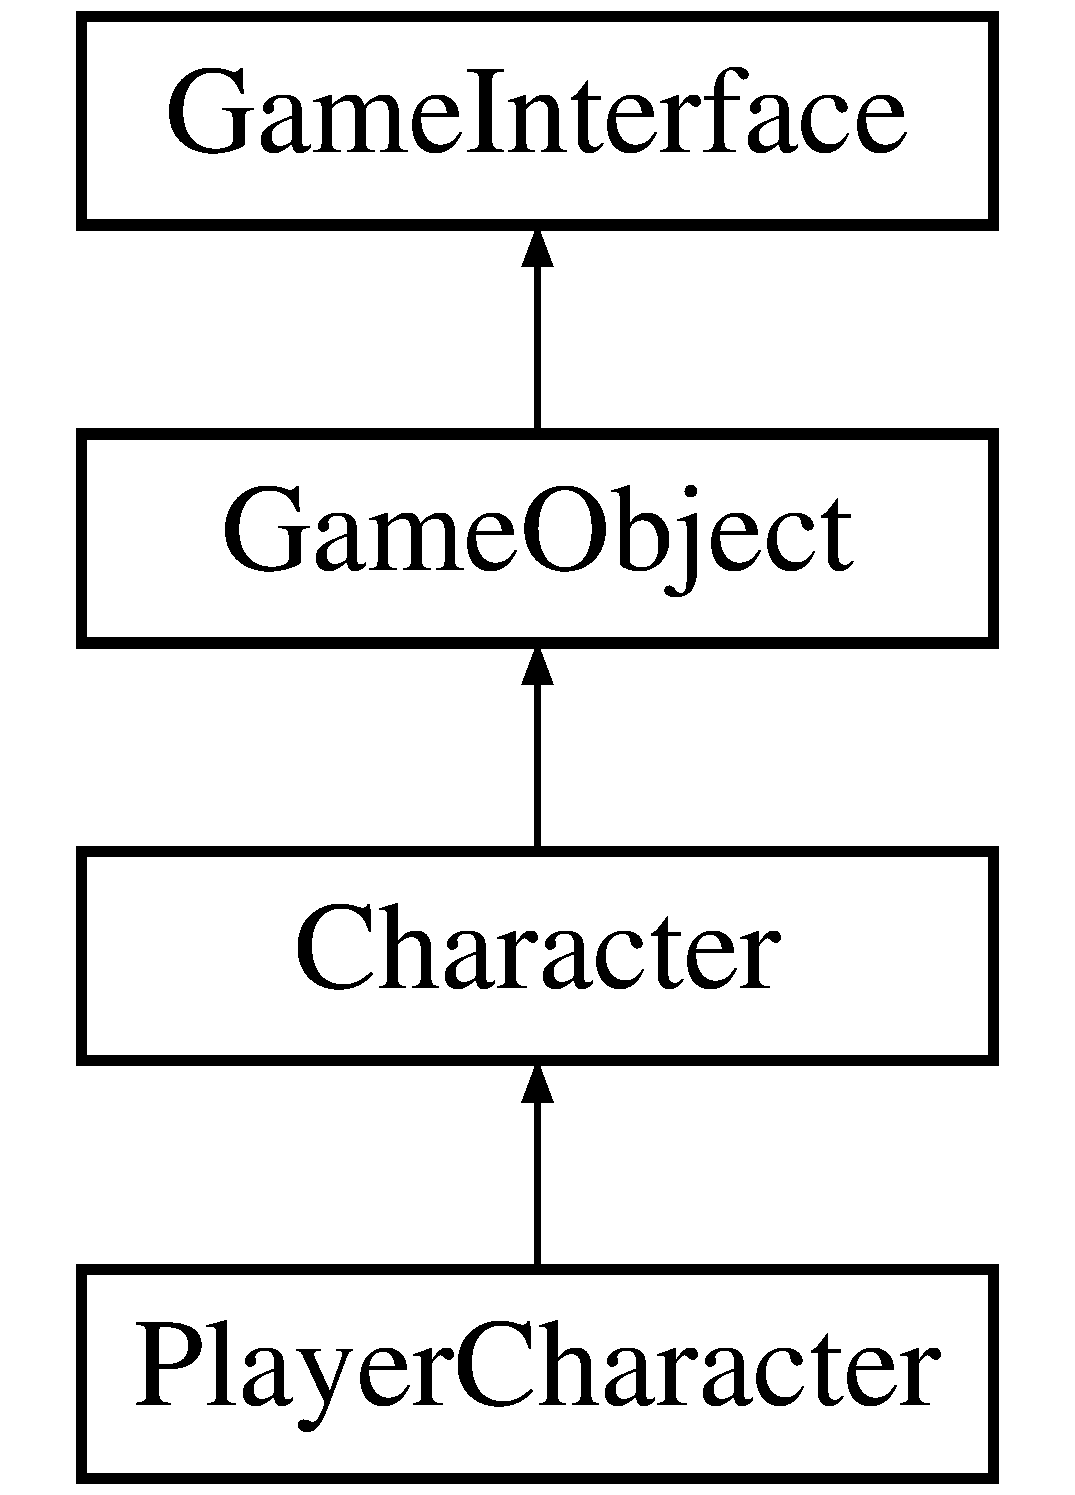
\includegraphics[height=4.000000cm]{class_player_character}
\end{center}
\end{figure}
\subsection*{Public Member Functions}
\begin{DoxyCompactItemize}
\item 
\hyperlink{class_player_character_af3ac12a41f58d860fb716138578bd95f}{Player\-Character} ()
\item 
\hyperlink{class_player_character_a39481690d96f66691b7a2f85a305f1f3}{Player\-Character} (const \hyperlink{class_player_character}{Player\-Character} \&other)
\item 
\hyperlink{class_player_character_aea36ba3a5672379d3b1daa80eb953de6}{Player\-Character} (\hyperlink{class_player_character}{Player\-Character} \&\&other)
\item 
\hyperlink{class_player_character_a08c4626862a0bf81f7dc8de90e883c1c}{Player\-Character} (const \hyperlink{struct_asset_file}{Asset\-File} \&image\-File, float \hyperlink{class_game_object_ac4637e122291be2421c851e2a87fb968}{size}, const \hyperlink{struct_position}{Position}$<$ float $>$ \&\hyperlink{class_game_object_a6858e668e7d2c5ded850b952aaacd905}{loc}, string \hyperlink{class_character_a2d423654566d1bf2160fef74bf04cc84}{name}, \hyperlink{_character_data_8h_a0e5ce1612c1e71823c97a9cd734de339}{Reaction} \hyperlink{class_character_a579933775b2e4e97465bacb09c4e87f5}{reaction}, \hyperlink{_character_data_8h_acbff4d7298e294294555d39178aad448}{Do\-A} \hyperlink{class_character_ac83b99be690bb41b7fae53e9457838c6}{alive}, \hyperlink{_character_data_8h_aacbb008a93d24b04a8779bbdbd8880b5}{Character\-State} \hyperlink{class_character_ac20f1ebda238017ddc245ecdce827037}{state}, unsigned \hyperlink{class_character_ae8c0d82624dc3a171e2c3b42c699151e}{health}, unsigned \hyperlink{class_character_ae6a140637ffe5004179d90a0e04a411b}{damage}, bool monitor\-Velocity, const \hyperlink{struct_asset_file}{Asset\-File} \&projectile\-Image\-File)
\item 
\hyperlink{class_player_character_a86f9249d7ef692f6647ffba3ae033cc0}{Player\-Character} (\hyperlink{class_fast_rand}{Fast\-Rand}$<$ int $>$ rand)
\item 
\hyperlink{class_player_character_a4915330a9f743156b6860a97e6d68e28}{$\sim$\-Player\-Character} ()
\item 
\hyperlink{class_player_character}{Player\-Character} \& \hyperlink{class_player_character_a3b949510e58a60e13e1a71d6c070c22b}{operator=} (const \hyperlink{class_player_character}{Player\-Character} \&rhs)
\item 
\hyperlink{class_player_character}{Player\-Character} \& \hyperlink{class_player_character_af33d69dba65288508b4291ae6aaa1aa3}{operator=} (\hyperlink{class_player_character}{Player\-Character} \&\&rhs)
\item 
void \hyperlink{class_player_character_a067c5b11f7deafd448726ec4ac294b03}{operator()} ()
\item 
void \hyperlink{class_player_character_a1cf7079c60a26c188cf4ed7043a2c9b3}{operator()} (\hyperlink{class_game_object}{Game\-Object} $\ast$other)
\item 
void \hyperlink{class_player_character_a6e9ba6daca1de1e325850f78f3c3bbc9}{move\-New\-Direction} (\hyperlink{struct_vectr}{Vectr}$<$ float $>$ new\-Direction) override
\item 
void \hyperlink{class_player_character_a0c82549ee968726256b518e89b78c605}{move\-Random\-Direction} () override
\item 
void \hyperlink{class_player_character_ac96dd84cef7668557321edc5b251c97c}{default\-Behaviors} () override
\item 
void \hyperlink{class_player_character_af7a8c30b3f40a698c28b095a299657ab}{ai\-Behaviors} () override
\item 
void \hyperlink{class_player_character_a646ce764c65c544fe4b76912b3fd15e5}{fire} ()
\item 
void \hyperlink{class_player_character_acb7767ff11d007399561aeb3445c38b8}{fire} (const \hyperlink{class_character}{Character} $\ast$at\-Enemy)
\item 
void \hyperlink{class_player_character_ab67b7f795e75b73027620483bea2871b}{jump} ()
\item 
void \hyperlink{class_player_character_a2ac275d3de97c5ecc260e93e0585168a}{update} () override
\item 
void \hyperlink{class_player_character_aac83579c2f552973e71008c1b1e01b1d}{text\-Description} (ostream $\ast$write\-To) const 
\item 
void \hyperlink{class_player_character_a0f0464366a0ab7b51d0000f14ad50485}{print\-Positition} ()
\end{DoxyCompactItemize}
\subsection*{Protected Attributes}
\begin{DoxyCompactItemize}
\item 
\hyperlink{class_weapon}{Weapon} \hyperlink{class_player_character_aebf48777d82418e8aa2a01747a117621}{weapon}
\item 
bool \hyperlink{class_player_character_a278a86804d9b5e8eddc66550f9fa82b6}{move\-Flag} = false
\begin{DoxyCompactList}\small\item\em A boolean flag which, when set to true, indicated that this \hyperlink{class_player_character}{Player\-Character} should \hyperlink{class_game_object_aebf4e54c90de73d56186beaebead1ccc}{move()} on the next call to update. \end{DoxyCompactList}\end{DoxyCompactItemize}
\subsection*{Additional Inherited Members}


\subsection{Detailed Description}
A class which serves as the basic template for just about any person in the game world, whether player or npc. 

Definition at line 24 of file Player\-Character.\-h.



\subsection{Constructor \& Destructor Documentation}
\hypertarget{class_player_character_af3ac12a41f58d860fb716138578bd95f}{\index{Player\-Character@{Player\-Character}!Player\-Character@{Player\-Character}}
\index{Player\-Character@{Player\-Character}!PlayerCharacter@{Player\-Character}}
\subsubsection[{Player\-Character}]{\setlength{\rightskip}{0pt plus 5cm}Player\-Character\-::\-Player\-Character (
\begin{DoxyParamCaption}
{}
\end{DoxyParamCaption}
)}}\label{class_player_character_af3ac12a41f58d860fb716138578bd95f}
Constructs a default \hyperlink{class_player_character}{Player\-Character}. 

Definition at line 14 of file Player\-Character.\-cpp.

\hypertarget{class_player_character_a39481690d96f66691b7a2f85a305f1f3}{\index{Player\-Character@{Player\-Character}!Player\-Character@{Player\-Character}}
\index{Player\-Character@{Player\-Character}!PlayerCharacter@{Player\-Character}}
\subsubsection[{Player\-Character}]{\setlength{\rightskip}{0pt plus 5cm}Player\-Character\-::\-Player\-Character (
\begin{DoxyParamCaption}
\item[{const {\bf Player\-Character} \&}]{other}
\end{DoxyParamCaption}
)}}\label{class_player_character_a39481690d96f66691b7a2f85a305f1f3}
Copy constructor for \hyperlink{class_player_character}{Player\-Character}


\begin{DoxyParams}{Parameters}
{\em other} & \hyperlink{class_player_character}{Player\-Character} to be copied\\
\hline
\end{DoxyParams}
Copy constructor for \hyperlink{class_player_character}{Player\-Character}


\begin{DoxyParams}{Parameters}
{\em other} & The \hyperlink{class_player_character}{Player\-Character} to be copied \\
\hline
\end{DoxyParams}


Definition at line 24 of file Player\-Character.\-cpp.

\hypertarget{class_player_character_aea36ba3a5672379d3b1daa80eb953de6}{\index{Player\-Character@{Player\-Character}!Player\-Character@{Player\-Character}}
\index{Player\-Character@{Player\-Character}!PlayerCharacter@{Player\-Character}}
\subsubsection[{Player\-Character}]{\setlength{\rightskip}{0pt plus 5cm}Player\-Character\-::\-Player\-Character (
\begin{DoxyParamCaption}
\item[{{\bf Player\-Character} \&\&}]{other}
\end{DoxyParamCaption}
)}}\label{class_player_character_aea36ba3a5672379d3b1daa80eb953de6}
Move constructor for \hyperlink{class_player_character}{Player\-Character}


\begin{DoxyParams}{Parameters}
{\em other} & The \hyperlink{class_player_character}{Player\-Character} to be moved \\
\hline
\end{DoxyParams}


Definition at line 33 of file Player\-Character.\-cpp.

\hypertarget{class_player_character_a08c4626862a0bf81f7dc8de90e883c1c}{\index{Player\-Character@{Player\-Character}!Player\-Character@{Player\-Character}}
\index{Player\-Character@{Player\-Character}!PlayerCharacter@{Player\-Character}}
\subsubsection[{Player\-Character}]{\setlength{\rightskip}{0pt plus 5cm}Player\-Character\-::\-Player\-Character (
\begin{DoxyParamCaption}
\item[{const {\bf Asset\-File} \&}]{image\-File, }
\item[{float}]{size, }
\item[{const {\bf Position}$<$ float $>$ \&}]{loc, }
\item[{string}]{name, }
\item[{{\bf Reaction}}]{reaction, }
\item[{{\bf Do\-A}}]{alive, }
\item[{{\bf Character\-State}}]{state, }
\item[{unsigned}]{health, }
\item[{unsigned}]{damage, }
\item[{bool}]{monitor\-Velocity, }
\item[{const {\bf Asset\-File} \&}]{projectile\-Image\-File}
\end{DoxyParamCaption}
)}}\label{class_player_character_a08c4626862a0bf81f7dc8de90e883c1c}
Constructs a \hyperlink{class_player_character}{Player\-Character} based on the arguments given


\begin{DoxyParams}{Parameters}
{\em name} & The name of this \hyperlink{class_player_character}{Player\-Character} \\
\hline
{\em alive} & Whether this \hyperlink{class_player_character}{Player\-Character} is dead or alive \\
\hline
{\em state} & The Character\-State of this \hyperlink{class_player_character}{Player\-Character} \\
\hline
{\em health} & The \hyperlink{struct_health}{Health} of this \hyperlink{class_player_character}{Player\-Character} \\
\hline
{\em damage} & The \hyperlink{struct_damage}{Damage} capability of this \hyperlink{class_player_character}{Player\-Character} \\
\hline
\end{DoxyParams}


Definition at line 46 of file Player\-Character.\-cpp.

\hypertarget{class_player_character_a86f9249d7ef692f6647ffba3ae033cc0}{\index{Player\-Character@{Player\-Character}!Player\-Character@{Player\-Character}}
\index{Player\-Character@{Player\-Character}!PlayerCharacter@{Player\-Character}}
\subsubsection[{Player\-Character}]{\setlength{\rightskip}{0pt plus 5cm}Player\-Character\-::\-Player\-Character (
\begin{DoxyParamCaption}
\item[{{\bf Fast\-Rand}$<$ int $>$}]{rand}
\end{DoxyParamCaption}
)}}\label{class_player_character_a86f9249d7ef692f6647ffba3ae033cc0}
Constructs a randomized \hyperlink{class_player_character}{Player\-Character}. The client has to option to simply leave the argument rand\-Seed as 0, in which case the constructor will generate its own random number.


\begin{DoxyParams}{Parameters}
{\em rand} & A seed to initialize the random number generator\\
\hline
\end{DoxyParams}
Constructs a randomized \hyperlink{class_player_character}{Player\-Character}. The client has to option to simply leave the argument rand\-Seed as 0, in which case the constructor will generate its own random number.


\begin{DoxyParams}{Parameters}
{\em rand\-Seed} & A seed to initialize the random number generator \\
\hline
\end{DoxyParams}


Definition at line 57 of file Player\-Character.\-cpp.

\hypertarget{class_player_character_a4915330a9f743156b6860a97e6d68e28}{\index{Player\-Character@{Player\-Character}!$\sim$\-Player\-Character@{$\sim$\-Player\-Character}}
\index{$\sim$\-Player\-Character@{$\sim$\-Player\-Character}!PlayerCharacter@{Player\-Character}}
\subsubsection[{$\sim$\-Player\-Character}]{\setlength{\rightskip}{0pt plus 5cm}Player\-Character\-::$\sim$\-Player\-Character (
\begin{DoxyParamCaption}
{}
\end{DoxyParamCaption}
)}}\label{class_player_character_a4915330a9f743156b6860a97e6d68e28}
Destructor for \hyperlink{class_player_character}{Player\-Character} 

Definition at line 65 of file Player\-Character.\-cpp.



\subsection{Member Function Documentation}
\hypertarget{class_player_character_af7a8c30b3f40a698c28b095a299657ab}{\index{Player\-Character@{Player\-Character}!ai\-Behaviors@{ai\-Behaviors}}
\index{ai\-Behaviors@{ai\-Behaviors}!PlayerCharacter@{Player\-Character}}
\subsubsection[{ai\-Behaviors}]{\setlength{\rightskip}{0pt plus 5cm}void Player\-Character\-::ai\-Behaviors (
\begin{DoxyParamCaption}
{}
\end{DoxyParamCaption}
)\hspace{0.3cm}{\ttfamily [inline]}, {\ttfamily [override]}, {\ttfamily [virtual]}}}\label{class_player_character_af7a8c30b3f40a698c28b095a299657ab}


Reimplemented from \hyperlink{class_character_a7bd55d3615c1eb092f800d8634fa9695}{Character}.



Definition at line 136 of file Player\-Character.\-h.

\hypertarget{class_player_character_ac96dd84cef7668557321edc5b251c97c}{\index{Player\-Character@{Player\-Character}!default\-Behaviors@{default\-Behaviors}}
\index{default\-Behaviors@{default\-Behaviors}!PlayerCharacter@{Player\-Character}}
\subsubsection[{default\-Behaviors}]{\setlength{\rightskip}{0pt plus 5cm}void Player\-Character\-::default\-Behaviors (
\begin{DoxyParamCaption}
{}
\end{DoxyParamCaption}
)\hspace{0.3cm}{\ttfamily [override]}, {\ttfamily [virtual]}}}\label{class_player_character_ac96dd84cef7668557321edc5b251c97c}
Each \hyperlink{class_game_object}{Game\-Object} can implement this to enable its default behaviors to run on a loop on a separate thread 

Reimplemented from \hyperlink{class_character_ac96260f4fd9b68a33919a65bc9da9bca}{Character}.



Definition at line 126 of file Player\-Character.\-cpp.

\hypertarget{class_player_character_a646ce764c65c544fe4b76912b3fd15e5}{\index{Player\-Character@{Player\-Character}!fire@{fire}}
\index{fire@{fire}!PlayerCharacter@{Player\-Character}}
\subsubsection[{fire}]{\setlength{\rightskip}{0pt plus 5cm}void Player\-Character\-::fire (
\begin{DoxyParamCaption}
{}
\end{DoxyParamCaption}
)\hspace{0.3cm}{\ttfamily [virtual]}}}\label{class_player_character_a646ce764c65c544fe4b76912b3fd15e5}
Fires the \hyperlink{class_player_character}{Player\-Character}'s weapon 

Reimplemented from \hyperlink{class_game_object_aefab5eddd7dfc186c7e5ba34bbefce41}{Game\-Object}.



Definition at line 131 of file Player\-Character.\-cpp.

\hypertarget{class_player_character_acb7767ff11d007399561aeb3445c38b8}{\index{Player\-Character@{Player\-Character}!fire@{fire}}
\index{fire@{fire}!PlayerCharacter@{Player\-Character}}
\subsubsection[{fire}]{\setlength{\rightskip}{0pt plus 5cm}void Player\-Character\-::fire (
\begin{DoxyParamCaption}
\item[{const {\bf Character} $\ast$}]{at\-Enemy}
\end{DoxyParamCaption}
)}}\label{class_player_character_acb7767ff11d007399561aeb3445c38b8}
Fires the \hyperlink{class_player_character}{Player\-Character}'s weapon


\begin{DoxyParams}{Parameters}
{\em at\-Enemy} & The enemy to attack \\
\hline
\end{DoxyParams}


Definition at line 136 of file Player\-Character.\-cpp.

\hypertarget{class_player_character_ab67b7f795e75b73027620483bea2871b}{\index{Player\-Character@{Player\-Character}!jump@{jump}}
\index{jump@{jump}!PlayerCharacter@{Player\-Character}}
\subsubsection[{jump}]{\setlength{\rightskip}{0pt plus 5cm}void Player\-Character\-::jump (
\begin{DoxyParamCaption}
{}
\end{DoxyParamCaption}
)\hspace{0.3cm}{\ttfamily [virtual]}}}\label{class_player_character_ab67b7f795e75b73027620483bea2871b}


Reimplemented from \hyperlink{class_game_object_aa8b87ef4a487c54c1d5b327c001b5c84}{Game\-Object}.



Definition at line 140 of file Player\-Character.\-cpp.

\hypertarget{class_player_character_a6e9ba6daca1de1e325850f78f3c3bbc9}{\index{Player\-Character@{Player\-Character}!move\-New\-Direction@{move\-New\-Direction}}
\index{move\-New\-Direction@{move\-New\-Direction}!PlayerCharacter@{Player\-Character}}
\subsubsection[{move\-New\-Direction}]{\setlength{\rightskip}{0pt plus 5cm}void Player\-Character\-::move\-New\-Direction (
\begin{DoxyParamCaption}
\item[{{\bf Vectr}$<$ float $>$}]{new\-Direction}
\end{DoxyParamCaption}
)\hspace{0.3cm}{\ttfamily [override]}}}\label{class_player_character_a6e9ba6daca1de1e325850f78f3c3bbc9}
Similar in function to \-::move\-New\-Direction(), but overridden to ensure the player cannot move more than once each time through the game loop 

Definition at line 115 of file Player\-Character.\-cpp.

\hypertarget{class_player_character_a0c82549ee968726256b518e89b78c605}{\index{Player\-Character@{Player\-Character}!move\-Random\-Direction@{move\-Random\-Direction}}
\index{move\-Random\-Direction@{move\-Random\-Direction}!PlayerCharacter@{Player\-Character}}
\subsubsection[{move\-Random\-Direction}]{\setlength{\rightskip}{0pt plus 5cm}void Player\-Character\-::move\-Random\-Direction (
\begin{DoxyParamCaption}
{}
\end{DoxyParamCaption}
)\hspace{0.3cm}{\ttfamily [inline]}, {\ttfamily [override]}, {\ttfamily [virtual]}}}\label{class_player_character_a0c82549ee968726256b518e89b78c605}
Overidden to ensure this has no functionality 

Reimplemented from \hyperlink{class_game_object_ac279191d7c42ca8ad3e1dd2baf5a9519}{Game\-Object}.



Definition at line 128 of file Player\-Character.\-h.

\hypertarget{class_player_character_a067c5b11f7deafd448726ec4ac294b03}{\index{Player\-Character@{Player\-Character}!operator()@{operator()}}
\index{operator()@{operator()}!PlayerCharacter@{Player\-Character}}
\subsubsection[{operator()}]{\setlength{\rightskip}{0pt plus 5cm}void Player\-Character\-::operator() (
\begin{DoxyParamCaption}
{}
\end{DoxyParamCaption}
)\hspace{0.3cm}{\ttfamily [virtual]}}}\label{class_player_character_a067c5b11f7deafd448726ec4ac294b03}
Overloads operator() for \hyperlink{class_player_character}{Player\-Character}. Possibly will be used to call \hyperlink{class_character_a457dab4f04550716888425da681b9f1f}{notify()}. T\-B\-D. 

Reimplemented from \hyperlink{class_character_a3c4dfc59865fe39251070cd0b92d34ac}{Character}.



Definition at line 100 of file Player\-Character.\-cpp.

\hypertarget{class_player_character_a1cf7079c60a26c188cf4ed7043a2c9b3}{\index{Player\-Character@{Player\-Character}!operator()@{operator()}}
\index{operator()@{operator()}!PlayerCharacter@{Player\-Character}}
\subsubsection[{operator()}]{\setlength{\rightskip}{0pt plus 5cm}void Player\-Character\-::operator() (
\begin{DoxyParamCaption}
\item[{{\bf Game\-Object} $\ast$}]{other}
\end{DoxyParamCaption}
)\hspace{0.3cm}{\ttfamily [virtual]}}}\label{class_player_character_a1cf7079c60a26c188cf4ed7043a2c9b3}
Overloads the overload of operator(). The actual implementation and uses for this are still undecided.


\begin{DoxyParams}{Parameters}
{\em other} & A reference to another \hyperlink{class_player_character}{Player\-Character}\\
\hline
\end{DoxyParams}
Overloads the overload of operator(). The actual implementation and uses for this are still undecided.


\begin{DoxyParams}{Parameters}
{\em other\-Character} & A reference to another \hyperlink{class_player_character}{Player\-Character} \\
\hline
\end{DoxyParams}


Reimplemented from \hyperlink{class_character_a6dde2dd17bfd31ea6e008d83bdcd3188}{Character}.



Definition at line 111 of file Player\-Character.\-cpp.

\hypertarget{class_player_character_a3b949510e58a60e13e1a71d6c070c22b}{\index{Player\-Character@{Player\-Character}!operator=@{operator=}}
\index{operator=@{operator=}!PlayerCharacter@{Player\-Character}}
\subsubsection[{operator=}]{\setlength{\rightskip}{0pt plus 5cm}{\bf Player\-Character} \& Player\-Character\-::operator= (
\begin{DoxyParamCaption}
\item[{const {\bf Player\-Character} \&}]{rhs}
\end{DoxyParamCaption}
)}}\label{class_player_character_a3b949510e58a60e13e1a71d6c070c22b}
Assignment operator overload (copy)


\begin{DoxyParams}{Parameters}
{\em rhs} & The right hand side argument (which will be copied) \\
\hline
\end{DoxyParams}


Definition at line 73 of file Player\-Character.\-cpp.

\hypertarget{class_player_character_af33d69dba65288508b4291ae6aaa1aa3}{\index{Player\-Character@{Player\-Character}!operator=@{operator=}}
\index{operator=@{operator=}!PlayerCharacter@{Player\-Character}}
\subsubsection[{operator=}]{\setlength{\rightskip}{0pt plus 5cm}{\bf Player\-Character} \& Player\-Character\-::operator= (
\begin{DoxyParamCaption}
\item[{{\bf Player\-Character} \&\&}]{rhs}
\end{DoxyParamCaption}
)}}\label{class_player_character_af33d69dba65288508b4291ae6aaa1aa3}
Assignment operator overload (move)


\begin{DoxyParams}{Parameters}
{\em rhs} & The right hand side argument (which will be moved) \\
\hline
\end{DoxyParams}


Definition at line 87 of file Player\-Character.\-cpp.

\hypertarget{class_player_character_a0f0464366a0ab7b51d0000f14ad50485}{\index{Player\-Character@{Player\-Character}!print\-Positition@{print\-Positition}}
\index{print\-Positition@{print\-Positition}!PlayerCharacter@{Player\-Character}}
\subsubsection[{print\-Positition}]{\setlength{\rightskip}{0pt plus 5cm}void Player\-Character\-::print\-Positition (
\begin{DoxyParamCaption}
{}
\end{DoxyParamCaption}
)}}\label{class_player_character_a0f0464366a0ab7b51d0000f14ad50485}


Definition at line 164 of file Player\-Character.\-cpp.

\hypertarget{class_player_character_aac83579c2f552973e71008c1b1e01b1d}{\index{Player\-Character@{Player\-Character}!text\-Description@{text\-Description}}
\index{text\-Description@{text\-Description}!PlayerCharacter@{Player\-Character}}
\subsubsection[{text\-Description}]{\setlength{\rightskip}{0pt plus 5cm}void Player\-Character\-::text\-Description (
\begin{DoxyParamCaption}
\item[{ostream $\ast$}]{write\-To}
\end{DoxyParamCaption}
) const\hspace{0.3cm}{\ttfamily [virtual]}}}\label{class_player_character_aac83579c2f552973e71008c1b1e01b1d}
Writes a formatted text description of this \hyperlink{class_player_character}{Player\-Character} into the desired output stream 

Reimplemented from \hyperlink{class_character_a2ab1090f959f0c66b098e0463d4c1bdd}{Character}.



Definition at line 160 of file Player\-Character.\-cpp.

\hypertarget{class_player_character_a2ac275d3de97c5ecc260e93e0585168a}{\index{Player\-Character@{Player\-Character}!update@{update}}
\index{update@{update}!PlayerCharacter@{Player\-Character}}
\subsubsection[{update}]{\setlength{\rightskip}{0pt plus 5cm}void Player\-Character\-::update (
\begin{DoxyParamCaption}
{}
\end{DoxyParamCaption}
)\hspace{0.3cm}{\ttfamily [override]}, {\ttfamily [virtual]}}}\label{class_player_character_a2ac275d3de97c5ecc260e93e0585168a}


Reimplemented from \hyperlink{class_game_object_adad7d284b670db722a2fda8e6a7997e3}{Game\-Object}.



Definition at line 150 of file Player\-Character.\-cpp.



\subsection{Member Data Documentation}
\hypertarget{class_player_character_a278a86804d9b5e8eddc66550f9fa82b6}{\index{Player\-Character@{Player\-Character}!move\-Flag@{move\-Flag}}
\index{move\-Flag@{move\-Flag}!PlayerCharacter@{Player\-Character}}
\subsubsection[{move\-Flag}]{\setlength{\rightskip}{0pt plus 5cm}bool Player\-Character\-::move\-Flag = false\hspace{0.3cm}{\ttfamily [protected]}}}\label{class_player_character_a278a86804d9b5e8eddc66550f9fa82b6}


A boolean flag which, when set to true, indicated that this \hyperlink{class_player_character}{Player\-Character} should \hyperlink{class_game_object_aebf4e54c90de73d56186beaebead1ccc}{move()} on the next call to update. 



Definition at line 35 of file Player\-Character.\-h.

\hypertarget{class_player_character_aebf48777d82418e8aa2a01747a117621}{\index{Player\-Character@{Player\-Character}!weapon@{weapon}}
\index{weapon@{weapon}!PlayerCharacter@{Player\-Character}}
\subsubsection[{weapon}]{\setlength{\rightskip}{0pt plus 5cm}{\bf Weapon} Player\-Character\-::weapon\hspace{0.3cm}{\ttfamily [protected]}}}\label{class_player_character_aebf48777d82418e8aa2a01747a117621}


Definition at line 28 of file Player\-Character.\-h.



The documentation for this class was generated from the following files\-:\begin{DoxyCompactItemize}
\item 
/\-Volumes/\-O\-S X H\-D\-D/\-Users/\-Adam/\-Developer/\-Sprite\-Fight/\-World/\hyperlink{_player_character_8h}{Player\-Character.\-h}\item 
/\-Volumes/\-O\-S X H\-D\-D/\-Users/\-Adam/\-Developer/\-Sprite\-Fight/\-World/\hyperlink{_player_character_8cpp}{Player\-Character.\-cpp}\end{DoxyCompactItemize}

\hypertarget{struct_pos2}{\section{Pos2$<$ N $>$ Struct Template Reference}
\label{struct_pos2}\index{Pos2$<$ N $>$@{Pos2$<$ N $>$}}
}


{\ttfamily \#include $<$Position.\-hpp$>$}

Inheritance diagram for Pos2$<$ N $>$\-:\begin{figure}[H]
\begin{center}
\leavevmode
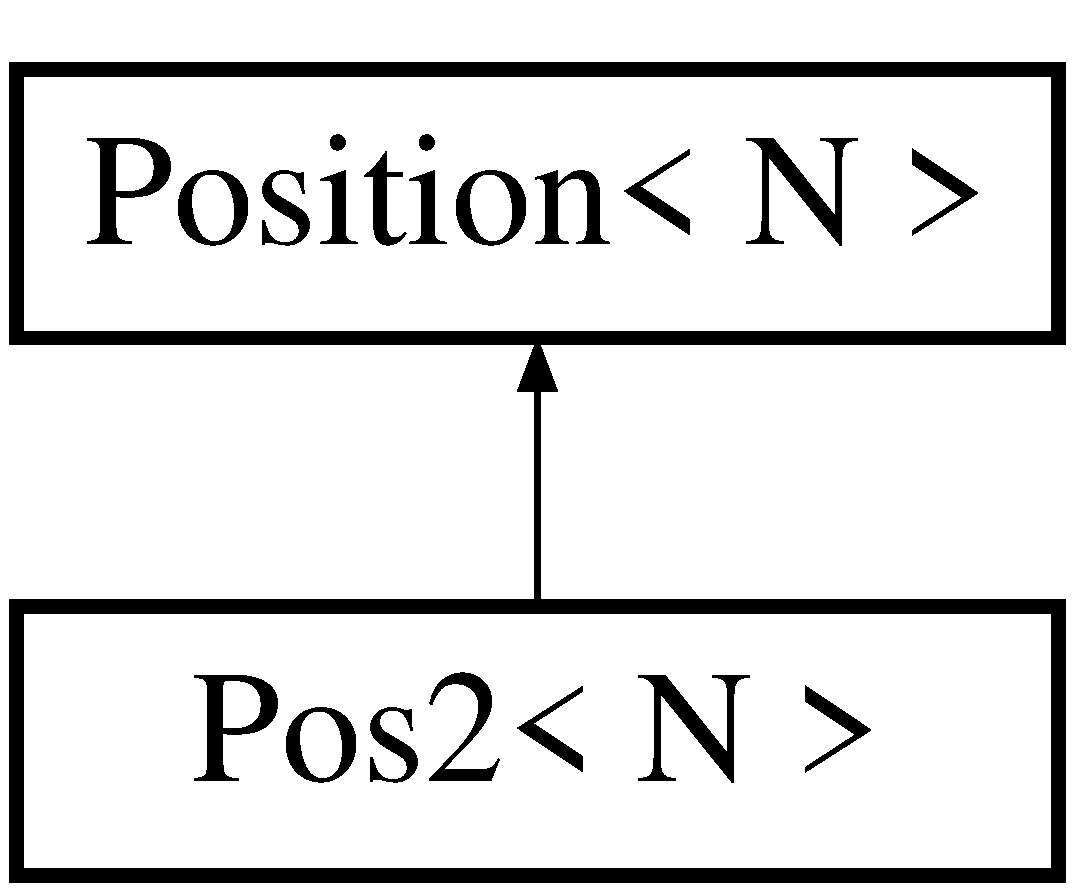
\includegraphics[height=2.000000cm]{struct_pos2}
\end{center}
\end{figure}
\subsection*{Public Member Functions}
\begin{DoxyCompactItemize}
\item 
\hyperlink{struct_pos2_af66901093e4a4ed4af0315a5555df3ff}{Pos2} ()
\item 
\hyperlink{struct_pos2_a34523a174500233d5f7222928e6fd1f1}{Pos2} (const \hyperlink{struct_position}{Position}$<$ N $>$ \&pos)
\item 
\hyperlink{struct_pos2_ae366b3cb5f89bda2a574490caddc2320}{Pos2} (const \hyperlink{struct_position}{Position}$<$ N $>$ \&pos, const \hyperlink{struct_bounds_check}{Bounds\-Check}$<$ N $>$ \&check)
\item 
\hyperlink{struct_pos2_aa272160e1bdc4cc04a2cb19351acf2dc}{Pos2} (const \hyperlink{struct_bounds_check}{Bounds\-Check}$<$ N $>$ \&check)
\item 
\hyperlink{struct_pos2_ae85aa637e77fc1c30b98eee7884f677a}{Pos2} (N n)
\item 
\hyperlink{struct_pos2_a746cc704e8b447b9f8e0037df6b704ba}{Pos2} (N n, const \hyperlink{struct_bounds_check}{Bounds\-Check}$<$ N $>$ \&check)
\item 
{\footnotesize template$<$typename R $>$ }\\\hyperlink{struct_pos2_a8c12e1e032bae75160901b5a59acd86f}{Pos2} (\hyperlink{class_fast_rand}{Fast\-Rand}$<$ R $>$ \&rand)
\item 
{\footnotesize template$<$typename R $>$ }\\\hyperlink{struct_pos2_ad763268dd2c65d60f0279b55f4079d31}{Pos2} (\hyperlink{class_fast_rand}{Fast\-Rand}$<$ R $>$ \&rand, const \hyperlink{struct_bounds_check}{Bounds\-Check}$<$ N $>$ \&check)
\item 
\hyperlink{struct_pos2_a6b88fd90d4b9173a4d95f8f91484f3fd}{Pos2} (const \hyperlink{struct_pos2}{Pos2} \&other)
\item 
\hyperlink{struct_pos2_aa35a42de65893664396cc6a584d3a936}{Pos2} (const \hyperlink{struct_pos2}{Pos2} \&other, const \hyperlink{struct_bounds_check}{Bounds\-Check}$<$ N $>$ \&check)
\item 
\hyperlink{struct_pos2_a7b2614b7ddcf0c3f0a3bc591ae5480dc}{Pos2} (\hyperlink{struct_pos2}{Pos2} \&\&other)
\item 
\hyperlink{struct_pos2_a235c965af4114604aac09c036f08d3e8}{Pos2} (\hyperlink{struct_pos2}{Pos2} \&\&other, const \hyperlink{struct_bounds_check}{Bounds\-Check}$<$ N $>$ \&check)
\item 
\hyperlink{struct_pos2_ad54b348d074c145a7d6abba6d571846b}{Pos2} (N \hyperlink{struct_position_af908be922fc88d89d81be7d08d06f761}{x}, N \hyperlink{struct_position_af434f54a0aad8bbfc3806ebdd197aa3b}{y}, N \hyperlink{struct_position_ac430da98504c2d4fd685c0363d728474}{z})
\item 
\hyperlink{struct_pos2_af46209c7d52909c4525d49554f000668}{Pos2} (N \hyperlink{struct_position_af908be922fc88d89d81be7d08d06f761}{x}, N \hyperlink{struct_position_af434f54a0aad8bbfc3806ebdd197aa3b}{y}, N \hyperlink{struct_position_ac430da98504c2d4fd685c0363d728474}{z}, const \hyperlink{struct_bounds_check}{Bounds\-Check}$<$ N $>$ \&check)
\item 
virtual \hyperlink{struct_pos2_a638367184a0bc381cd15155e375e5e92}{$\sim$\-Pos2} ()
\item 
\hyperlink{struct_pos2}{Pos2} \& \hyperlink{struct_pos2_a38a5bcfaf5dba1e92cc9d7889daa1721}{operator=} (const \hyperlink{struct_pos2}{Pos2} \&rhs)
\item 
\hyperlink{struct_pos2}{Pos2} \& \hyperlink{struct_pos2_ad2be6bde52c8afa3897beadb2608e3a4}{operator=} (\hyperlink{struct_pos2}{Pos2} \&\&rhs)
\item 
\hyperlink{struct_pos2}{Pos2} \& \hyperlink{struct_pos2_a340228a5c2933605e488596eed7fdc16}{operator=} (const \hyperlink{struct_position}{Position}$<$ N $>$ \&rhs)
\item 
\hyperlink{struct_pos2}{Pos2} \& \hyperlink{struct_pos2_a02609d7ec3de3cb29b237ae280cd4d03}{operator=} (\hyperlink{struct_position}{Position}$<$ N $>$ \&\&rhs)
\item 
bool \hyperlink{struct_pos2_ae8efa7bdafbf75b2a9e689df1f345a44}{operator==} (const \hyperlink{struct_pos2}{Pos2} \&rhs) const 
\item 
bool \hyperlink{struct_pos2_aa255eeb0bcc2c92bc7aeb7a6babb7f71}{operator==} (\hyperlink{struct_pos2}{Pos2} \&rhs) const 
\item 
bool \hyperlink{struct_pos2_aaa70e9e703ecf5cf3c85ab7e262ad2cb}{operator==} (const \hyperlink{struct_position}{Position}$<$ N $>$ \&rhs) const 
\item 
bool \hyperlink{struct_pos2_ad79c54f096426bf141a40af32e88d7d3}{operator==} (\hyperlink{struct_position}{Position}$<$ N $>$ \&rhs) const 
\item 
bool \hyperlink{struct_pos2_a1470c730d1dd5195aa301f81cb9f0a07}{operator!=} (\hyperlink{struct_pos2}{Pos2} \&rhs) const 
\item 
bool \hyperlink{struct_pos2_a03fd764f516526f65ad6faa6e2e9da52}{operator!=} (const \hyperlink{struct_pos2}{Pos2} \&rhs) const 
\item 
bool \hyperlink{struct_pos2_aabe6423f2d519d015c022fe8aedd2da9}{operator!=} (\hyperlink{struct_position}{Position}$<$ N $>$ \&rhs) const 
\item 
bool \hyperlink{struct_pos2_ae519d026266e7c63cede223ba78d68cf}{operator!=} (const \hyperlink{struct_position}{Position}$<$ N $>$ \&rhs) const 
\item 
\hyperlink{struct_pos2}{Pos2} \hyperlink{struct_pos2_a4965bba4823fd63b07ac6bf2288e354c}{operator+} (const \hyperlink{struct_pos2}{Pos2} \&rhs) const 
\item 
\hyperlink{struct_pos2}{Pos2} \hyperlink{struct_pos2_aa48d970911091f26baa779003392d654}{operator+} (const \hyperlink{struct_position}{Position}$<$ N $>$ \&rhs) const 
\item 
\hyperlink{struct_pos2}{Pos2} \hyperlink{struct_pos2_a8491e1dd62f258d99e607eeccb193124}{operator-\/} (const \hyperlink{struct_pos2}{Pos2} \&rhs) const 
\item 
\hyperlink{struct_pos2}{Pos2} \hyperlink{struct_pos2_a205a04ea6ab7f1d055a1f00c6602ae08}{operator-\/} (const \hyperlink{struct_position}{Position}$<$ N $>$ \&rhs) const 
\item 
const \hyperlink{struct_position}{Position}$<$ N $>$ $\ast$ \hyperlink{struct_pos2_a37c3a0998d4423f50fc09e074fc01522}{get\-Current} ()
\item 
const deque$<$ \hyperlink{struct_position}{Position}$<$ N $>$ $>$ $\ast$ \hyperlink{struct_pos2_ab9730d7c07f3aed458574ad9f63a7035}{get\-History} ()
\item 
void \hyperlink{struct_pos2_ae98c349465ab4c1085504649413f729b}{set\-All} (const N \hyperlink{struct_position_af908be922fc88d89d81be7d08d06f761}{x}, const N \hyperlink{struct_position_af434f54a0aad8bbfc3806ebdd197aa3b}{y}, const N \hyperlink{struct_position_ac430da98504c2d4fd685c0363d728474}{z})
\item 
void \hyperlink{struct_pos2_a5a26baf8ed6060892131a6e5341f0f3f}{set\-All} (const N \hyperlink{struct_position_af908be922fc88d89d81be7d08d06f761}{x}, const N \hyperlink{struct_position_af434f54a0aad8bbfc3806ebdd197aa3b}{y}, const N \hyperlink{struct_position_ac430da98504c2d4fd685c0363d728474}{z}, const \hyperlink{struct_bounds_check}{Bounds\-Check}$<$ N $>$ \&check)
\item 
void \hyperlink{struct_pos2_a65721a562cff5cbcbf023f4669783f32}{set\-All} (const \hyperlink{struct_position}{Position}$<$ N $>$ \&other)
\item 
void \hyperlink{struct_pos2_a830495035e3981da9e298db636b7f26a}{set\-All} (const \hyperlink{struct_position}{Position}$<$ N $>$ \&other, const \hyperlink{struct_bounds_check}{Bounds\-Check}$<$ N $>$ \&check)
\item 
void \hyperlink{struct_pos2_aef9a2916285822cc7a3c8741bd38ddf7}{set\-All} (const N n)
\item 
void \hyperlink{struct_pos2_ae08b2b8134a316cc26da0c2b96bf4f14}{set\-All} (const N n, const \hyperlink{struct_bounds_check}{Bounds\-Check}$<$ N $>$ \&check)
\item 
void \hyperlink{struct_pos2_a16c48d5f21dfe7e00c1c2cb27e0e13f0}{set\-All\-Zero} ()
\item 
void \hyperlink{struct_pos2_abbed99ee02ea50c3dc1053671b7331bb}{set\-X} (const N \hyperlink{struct_position_af908be922fc88d89d81be7d08d06f761}{x})
\item 
void \hyperlink{struct_pos2_a8ff8dc117956df7acb135c17731133ec}{set\-X} (const N \hyperlink{struct_position_af908be922fc88d89d81be7d08d06f761}{x}, const \hyperlink{struct_bounds_check}{Bounds\-Check}$<$ N $>$ \&check)
\item 
void \hyperlink{struct_pos2_a82ddb6fab8b028a52d53bb28f03b6119}{set\-Y} (const N \hyperlink{struct_position_af434f54a0aad8bbfc3806ebdd197aa3b}{y})
\item 
void \hyperlink{struct_pos2_a6ebb86ee57ab1467de7e5440d8e6358c}{set\-Y} (const N \hyperlink{struct_position_af434f54a0aad8bbfc3806ebdd197aa3b}{y}, const \hyperlink{struct_bounds_check}{Bounds\-Check}$<$ N $>$ \&check)
\item 
void \hyperlink{struct_pos2_aaa8e7d737a065e7ca846791ff31ea25c}{set\-Z} (const N \hyperlink{struct_position_ac430da98504c2d4fd685c0363d728474}{z})
\item 
void \hyperlink{struct_pos2_af5641ffd9e8b359f7f80321c5d7ddbf5}{set\-Z} (const N \hyperlink{struct_position_ac430da98504c2d4fd685c0363d728474}{z}, const \hyperlink{struct_bounds_check}{Bounds\-Check}$<$ N $>$ \&check)
\item 
void \hyperlink{struct_pos2_af1b35a8b928bea9c73c49ff384b35a4a}{x\-\_\-plus\-\_\-one} ()
\item 
void \hyperlink{struct_pos2_a95c416fe3b7b2171df1daeb36416e62a}{x\-\_\-plus\-\_\-one} (const \hyperlink{struct_bounds_check}{Bounds\-Check}$<$ N $>$ \&check)
\item 
void \hyperlink{struct_pos2_a0f132fb8ed0c2e7092614cde74ccde27}{x\-\_\-minus\-\_\-one} ()
\item 
void \hyperlink{struct_pos2_a6c0daea0c94397af825a3e943665c41a}{x\-\_\-minus\-\_\-one} (const \hyperlink{struct_bounds_check}{Bounds\-Check}$<$ N $>$ \&check)
\item 
void \hyperlink{struct_pos2_a4bd636102c60fc9e19cb91ffc8dd68bc}{y\-\_\-plus\-\_\-one} ()
\item 
void \hyperlink{struct_pos2_abc24856ae8ef5a4c7bac195193f67e06}{y\-\_\-plus\-\_\-one} (const \hyperlink{struct_bounds_check}{Bounds\-Check}$<$ N $>$ \&check)
\item 
void \hyperlink{struct_pos2_ae42c57baaa5f3c59565a3d864a6c06f1}{y\-\_\-minus\-\_\-one} ()
\item 
void \hyperlink{struct_pos2_a90279c33382f18b737dc2afa901bb4ce}{y\-\_\-minus\-\_\-one} (const \hyperlink{struct_bounds_check}{Bounds\-Check}$<$ N $>$ \&check)
\item 
void \hyperlink{struct_pos2_ae333400e09bd51d4953bd37a6bc4fea9}{move\-Right} ()
\item 
void \hyperlink{struct_pos2_a8744dd1eb4d237f0a7b7c3cd000baed2}{move\-Left} ()
\item 
void \hyperlink{struct_pos2_a579238a3a5615ab36e2407aa6ce9177b}{move\-Up} ()
\item 
void \hyperlink{struct_pos2_abc5361e6f9349c9a5f847f9abd7047e9}{move\-Down} ()
\item 
void \hyperlink{struct_pos2_a815233851b548e25f8f4376f0cfee6f6}{move\-Up\-Right} ()
\item 
void \hyperlink{struct_pos2_a5c7870fae349b5d3a5d643f0ebf2c022}{move\-Up\-Left} ()
\item 
void \hyperlink{struct_pos2_adb6ee58f9bd32c327d3b24002c5cc0b4}{move\-Down\-Right} ()
\item 
void \hyperlink{struct_pos2_aa083f335d346e4f9afa5c4c41e253d46}{move\-Down\-Left} ()
\item 
void \hyperlink{struct_pos2_a3065dacbd8e42b36fd5af0775a9342d8}{modify} (N delta\-\_\-x, N delta\-\_\-y, N delta\-\_\-z)
\item 
void \hyperlink{struct_pos2_ab0ddc65822cce3935319977f3ab7c8e2}{modify} (N delta\-\_\-x, N delta\-\_\-y, N delta\-\_\-z, const \hyperlink{struct_bounds_check}{Bounds\-Check}$<$ N $>$ \&check)
\item 
void \hyperlink{struct_pos2_a8cb8d4f4d076ef9ecbb34bcb351ba8fa}{move\-Here} (N \hyperlink{struct_position_af908be922fc88d89d81be7d08d06f761}{x}, N \hyperlink{struct_position_af434f54a0aad8bbfc3806ebdd197aa3b}{y}, N \hyperlink{struct_position_ac430da98504c2d4fd685c0363d728474}{z})
\item 
void \hyperlink{struct_pos2_a2cf33b5575ca6cd5a02dbc92ee22fe7a}{move\-Here} (N \hyperlink{struct_position_af908be922fc88d89d81be7d08d06f761}{x}, N \hyperlink{struct_position_af434f54a0aad8bbfc3806ebdd197aa3b}{y}, N \hyperlink{struct_position_ac430da98504c2d4fd685c0363d728474}{z}, const \hyperlink{struct_bounds_check}{Bounds\-Check}$<$ N $>$ \&check)
\item 
void \hyperlink{struct_pos2_aca684f49b5e27317ea5580f467e5d34a}{move\-Here} (const \hyperlink{struct_pos2}{Pos2} \&other)
\item 
void \hyperlink{struct_pos2_a112150629c1c77a913f401e8948849b0}{move\-Here} (const \hyperlink{struct_position}{Position}$<$ N $>$ \&other)
\item 
void \hyperlink{struct_pos2_a6f1f873271a2ce51509f419faf52ed54}{move\-Here} (const \hyperlink{struct_pos2}{Pos2} \&other, const \hyperlink{struct_bounds_check}{Bounds\-Check}$<$ N $>$ \&check)
\item 
void \hyperlink{struct_pos2_aa743473a51150e91792af64c00153ed9}{move\-Here} (const \hyperlink{struct_position}{Position}$<$ N $>$ \&other, const \hyperlink{struct_bounds_check}{Bounds\-Check}$<$ N $>$ \&check)
\end{DoxyCompactItemize}
\subsection*{Protected Member Functions}
\begin{DoxyCompactItemize}
\item 
void \hyperlink{struct_pos2_a082aa8d85af22b1a8d671c8a44c3b0eb}{archive} ()
\end{DoxyCompactItemize}
\subsection*{Protected Attributes}
\begin{DoxyCompactItemize}
\item 
deque$<$ \hyperlink{struct_position}{Position}$<$ N $>$ $>$ $\ast$ \hyperlink{struct_pos2_ab0e6af6b5960554712bcb717518f6ac3}{past\-Positions}
\end{DoxyCompactItemize}
\subsection*{Additional Inherited Members}


\subsection{Detailed Description}
\subsubsection*{template$<$typename N$>$struct Pos2$<$ N $>$}

Similar to \hyperlink{struct_position}{Position}, but also holds copies of each of its previous states. 

Definition at line 561 of file Position.\-hpp.



\subsection{Constructor \& Destructor Documentation}
\hypertarget{struct_pos2_af66901093e4a4ed4af0315a5555df3ff}{\index{Pos2@{Pos2}!Pos2@{Pos2}}
\index{Pos2@{Pos2}!Pos2@{Pos2}}
\subsubsection[{Pos2}]{\setlength{\rightskip}{0pt plus 5cm}template$<$typename N$>$ {\bf Pos2}$<$ N $>$\-::{\bf Pos2} (
\begin{DoxyParamCaption}
{}
\end{DoxyParamCaption}
)\hspace{0.3cm}{\ttfamily [inline]}}}\label{struct_pos2_af66901093e4a4ed4af0315a5555df3ff}
Creates a \hyperlink{struct_pos2}{Pos2} with all coordinates initialized to 0 

Definition at line 589 of file Position.\-hpp.

\hypertarget{struct_pos2_a34523a174500233d5f7222928e6fd1f1}{\index{Pos2@{Pos2}!Pos2@{Pos2}}
\index{Pos2@{Pos2}!Pos2@{Pos2}}
\subsubsection[{Pos2}]{\setlength{\rightskip}{0pt plus 5cm}template$<$typename N$>$ {\bf Pos2}$<$ N $>$\-::{\bf Pos2} (
\begin{DoxyParamCaption}
\item[{const {\bf Position}$<$ N $>$ \&}]{pos}
\end{DoxyParamCaption}
)\hspace{0.3cm}{\ttfamily [inline]}}}\label{struct_pos2_a34523a174500233d5f7222928e6fd1f1}


Definition at line 591 of file Position.\-hpp.

\hypertarget{struct_pos2_ae366b3cb5f89bda2a574490caddc2320}{\index{Pos2@{Pos2}!Pos2@{Pos2}}
\index{Pos2@{Pos2}!Pos2@{Pos2}}
\subsubsection[{Pos2}]{\setlength{\rightskip}{0pt plus 5cm}template$<$typename N$>$ {\bf Pos2}$<$ N $>$\-::{\bf Pos2} (
\begin{DoxyParamCaption}
\item[{const {\bf Position}$<$ N $>$ \&}]{pos, }
\item[{const {\bf Bounds\-Check}$<$ N $>$ \&}]{check}
\end{DoxyParamCaption}
)\hspace{0.3cm}{\ttfamily [inline]}}}\label{struct_pos2_ae366b3cb5f89bda2a574490caddc2320}


Definition at line 593 of file Position.\-hpp.

\hypertarget{struct_pos2_aa272160e1bdc4cc04a2cb19351acf2dc}{\index{Pos2@{Pos2}!Pos2@{Pos2}}
\index{Pos2@{Pos2}!Pos2@{Pos2}}
\subsubsection[{Pos2}]{\setlength{\rightskip}{0pt plus 5cm}template$<$typename N$>$ {\bf Pos2}$<$ N $>$\-::{\bf Pos2} (
\begin{DoxyParamCaption}
\item[{const {\bf Bounds\-Check}$<$ N $>$ \&}]{check}
\end{DoxyParamCaption}
)\hspace{0.3cm}{\ttfamily [inline]}}}\label{struct_pos2_aa272160e1bdc4cc04a2cb19351acf2dc}
Creates a \hyperlink{struct_pos2}{Pos2} with all coordinates initialized to 0 

Definition at line 598 of file Position.\-hpp.

\hypertarget{struct_pos2_ae85aa637e77fc1c30b98eee7884f677a}{\index{Pos2@{Pos2}!Pos2@{Pos2}}
\index{Pos2@{Pos2}!Pos2@{Pos2}}
\subsubsection[{Pos2}]{\setlength{\rightskip}{0pt plus 5cm}template$<$typename N$>$ {\bf Pos2}$<$ N $>$\-::{\bf Pos2} (
\begin{DoxyParamCaption}
\item[{N}]{n}
\end{DoxyParamCaption}
)\hspace{0.3cm}{\ttfamily [inline]}}}\label{struct_pos2_ae85aa637e77fc1c30b98eee7884f677a}
Creates a \hyperlink{struct_pos2}{Pos2} with all coordinates initialized to n 

Definition at line 603 of file Position.\-hpp.

\hypertarget{struct_pos2_a746cc704e8b447b9f8e0037df6b704ba}{\index{Pos2@{Pos2}!Pos2@{Pos2}}
\index{Pos2@{Pos2}!Pos2@{Pos2}}
\subsubsection[{Pos2}]{\setlength{\rightskip}{0pt plus 5cm}template$<$typename N$>$ {\bf Pos2}$<$ N $>$\-::{\bf Pos2} (
\begin{DoxyParamCaption}
\item[{N}]{n, }
\item[{const {\bf Bounds\-Check}$<$ N $>$ \&}]{check}
\end{DoxyParamCaption}
)\hspace{0.3cm}{\ttfamily [inline]}}}\label{struct_pos2_a746cc704e8b447b9f8e0037df6b704ba}
Creates a \hyperlink{struct_pos2}{Pos2} with all coordinates initialized to n 

Definition at line 608 of file Position.\-hpp.

\hypertarget{struct_pos2_a8c12e1e032bae75160901b5a59acd86f}{\index{Pos2@{Pos2}!Pos2@{Pos2}}
\index{Pos2@{Pos2}!Pos2@{Pos2}}
\subsubsection[{Pos2}]{\setlength{\rightskip}{0pt plus 5cm}template$<$typename N$>$ template$<$typename R $>$ {\bf Pos2}$<$ N $>$\-::{\bf Pos2} (
\begin{DoxyParamCaption}
\item[{{\bf Fast\-Rand}$<$ R $>$ \&}]{rand}
\end{DoxyParamCaption}
)\hspace{0.3cm}{\ttfamily [inline]}}}\label{struct_pos2_a8c12e1e032bae75160901b5a59acd86f}
Creates a \hyperlink{struct_pos2}{Pos2} all coordinates randomized, with bounds set by check 

Definition at line 614 of file Position.\-hpp.

\hypertarget{struct_pos2_ad763268dd2c65d60f0279b55f4079d31}{\index{Pos2@{Pos2}!Pos2@{Pos2}}
\index{Pos2@{Pos2}!Pos2@{Pos2}}
\subsubsection[{Pos2}]{\setlength{\rightskip}{0pt plus 5cm}template$<$typename N$>$ template$<$typename R $>$ {\bf Pos2}$<$ N $>$\-::{\bf Pos2} (
\begin{DoxyParamCaption}
\item[{{\bf Fast\-Rand}$<$ R $>$ \&}]{rand, }
\item[{const {\bf Bounds\-Check}$<$ N $>$ \&}]{check}
\end{DoxyParamCaption}
)\hspace{0.3cm}{\ttfamily [inline]}}}\label{struct_pos2_ad763268dd2c65d60f0279b55f4079d31}
Creates a \hyperlink{struct_pos2}{Pos2} all coordinates randomized, with bounds set by check 

Definition at line 622 of file Position.\-hpp.

\hypertarget{struct_pos2_a6b88fd90d4b9173a4d95f8f91484f3fd}{\index{Pos2@{Pos2}!Pos2@{Pos2}}
\index{Pos2@{Pos2}!Pos2@{Pos2}}
\subsubsection[{Pos2}]{\setlength{\rightskip}{0pt plus 5cm}template$<$typename N$>$ {\bf Pos2}$<$ N $>$\-::{\bf Pos2} (
\begin{DoxyParamCaption}
\item[{const {\bf Pos2}$<$ N $>$ \&}]{other}
\end{DoxyParamCaption}
)\hspace{0.3cm}{\ttfamily [inline]}}}\label{struct_pos2_a6b88fd90d4b9173a4d95f8f91484f3fd}
Copy constructor for \hyperlink{struct_pos2}{Pos2} 

Definition at line 629 of file Position.\-hpp.

\hypertarget{struct_pos2_aa35a42de65893664396cc6a584d3a936}{\index{Pos2@{Pos2}!Pos2@{Pos2}}
\index{Pos2@{Pos2}!Pos2@{Pos2}}
\subsubsection[{Pos2}]{\setlength{\rightskip}{0pt plus 5cm}template$<$typename N$>$ {\bf Pos2}$<$ N $>$\-::{\bf Pos2} (
\begin{DoxyParamCaption}
\item[{const {\bf Pos2}$<$ N $>$ \&}]{other, }
\item[{const {\bf Bounds\-Check}$<$ N $>$ \&}]{check}
\end{DoxyParamCaption}
)\hspace{0.3cm}{\ttfamily [inline]}}}\label{struct_pos2_aa35a42de65893664396cc6a584d3a936}
Copy constructor for \hyperlink{struct_pos2}{Pos2} 

Definition at line 638 of file Position.\-hpp.

\hypertarget{struct_pos2_a7b2614b7ddcf0c3f0a3bc591ae5480dc}{\index{Pos2@{Pos2}!Pos2@{Pos2}}
\index{Pos2@{Pos2}!Pos2@{Pos2}}
\subsubsection[{Pos2}]{\setlength{\rightskip}{0pt plus 5cm}template$<$typename N$>$ {\bf Pos2}$<$ N $>$\-::{\bf Pos2} (
\begin{DoxyParamCaption}
\item[{{\bf Pos2}$<$ N $>$ \&\&}]{other}
\end{DoxyParamCaption}
)\hspace{0.3cm}{\ttfamily [inline]}}}\label{struct_pos2_a7b2614b7ddcf0c3f0a3bc591ae5480dc}
Move constructor for \hyperlink{struct_pos2}{Pos2} 

Definition at line 647 of file Position.\-hpp.

\hypertarget{struct_pos2_a235c965af4114604aac09c036f08d3e8}{\index{Pos2@{Pos2}!Pos2@{Pos2}}
\index{Pos2@{Pos2}!Pos2@{Pos2}}
\subsubsection[{Pos2}]{\setlength{\rightskip}{0pt plus 5cm}template$<$typename N$>$ {\bf Pos2}$<$ N $>$\-::{\bf Pos2} (
\begin{DoxyParamCaption}
\item[{{\bf Pos2}$<$ N $>$ \&\&}]{other, }
\item[{const {\bf Bounds\-Check}$<$ N $>$ \&}]{check}
\end{DoxyParamCaption}
)\hspace{0.3cm}{\ttfamily [inline]}}}\label{struct_pos2_a235c965af4114604aac09c036f08d3e8}
Move constructor for \hyperlink{struct_position}{Position} 

Definition at line 663 of file Position.\-hpp.

\hypertarget{struct_pos2_ad54b348d074c145a7d6abba6d571846b}{\index{Pos2@{Pos2}!Pos2@{Pos2}}
\index{Pos2@{Pos2}!Pos2@{Pos2}}
\subsubsection[{Pos2}]{\setlength{\rightskip}{0pt plus 5cm}template$<$typename N$>$ {\bf Pos2}$<$ N $>$\-::{\bf Pos2} (
\begin{DoxyParamCaption}
\item[{N}]{x, }
\item[{N}]{y, }
\item[{N}]{z}
\end{DoxyParamCaption}
)\hspace{0.3cm}{\ttfamily [inline]}}}\label{struct_pos2_ad54b348d074c145a7d6abba6d571846b}
Creates a \hyperlink{struct_pos2}{Pos2} with coordinates initialized to the given arguments


\begin{DoxyParams}{Parameters}
{\em x} & The x coordinate \\
\hline
{\em y} & The y coordinate \\
\hline
{\em z} & The z coordinate \\
\hline
\end{DoxyParams}


Definition at line 684 of file Position.\-hpp.

\hypertarget{struct_pos2_af46209c7d52909c4525d49554f000668}{\index{Pos2@{Pos2}!Pos2@{Pos2}}
\index{Pos2@{Pos2}!Pos2@{Pos2}}
\subsubsection[{Pos2}]{\setlength{\rightskip}{0pt plus 5cm}template$<$typename N$>$ {\bf Pos2}$<$ N $>$\-::{\bf Pos2} (
\begin{DoxyParamCaption}
\item[{N}]{x, }
\item[{N}]{y, }
\item[{N}]{z, }
\item[{const {\bf Bounds\-Check}$<$ N $>$ \&}]{check}
\end{DoxyParamCaption}
)\hspace{0.3cm}{\ttfamily [inline]}}}\label{struct_pos2_af46209c7d52909c4525d49554f000668}
Creates a \hyperlink{struct_pos2}{Pos2} with coordinates initialized to the given arguments


\begin{DoxyParams}{Parameters}
{\em x} & The x coordinate \\
\hline
{\em y} & The y coordinate \\
\hline
{\em z} & The z coordinate \\
\hline
\end{DoxyParams}


Definition at line 694 of file Position.\-hpp.

\hypertarget{struct_pos2_a638367184a0bc381cd15155e375e5e92}{\index{Pos2@{Pos2}!$\sim$\-Pos2@{$\sim$\-Pos2}}
\index{$\sim$\-Pos2@{$\sim$\-Pos2}!Pos2@{Pos2}}
\subsubsection[{$\sim$\-Pos2}]{\setlength{\rightskip}{0pt plus 5cm}template$<$typename N$>$ virtual {\bf Pos2}$<$ N $>$\-::$\sim${\bf Pos2} (
\begin{DoxyParamCaption}
{}
\end{DoxyParamCaption}
)\hspace{0.3cm}{\ttfamily [inline]}, {\ttfamily [virtual]}}}\label{struct_pos2_a638367184a0bc381cd15155e375e5e92}
Destructor for \hyperlink{struct_position}{Position} 

Definition at line 699 of file Position.\-hpp.



\subsection{Member Function Documentation}
\hypertarget{struct_pos2_a082aa8d85af22b1a8d671c8a44c3b0eb}{\index{Pos2@{Pos2}!archive@{archive}}
\index{archive@{archive}!Pos2@{Pos2}}
\subsubsection[{archive}]{\setlength{\rightskip}{0pt plus 5cm}template$<$typename N$>$ void {\bf Pos2}$<$ N $>$\-::archive (
\begin{DoxyParamCaption}
{}
\end{DoxyParamCaption}
)\hspace{0.3cm}{\ttfamily [inline]}, {\ttfamily [protected]}}}\label{struct_pos2_a082aa8d85af22b1a8d671c8a44c3b0eb}
Saves our current state 

Definition at line 575 of file Position.\-hpp.

\hypertarget{struct_pos2_a37c3a0998d4423f50fc09e074fc01522}{\index{Pos2@{Pos2}!get\-Current@{get\-Current}}
\index{get\-Current@{get\-Current}!Pos2@{Pos2}}
\subsubsection[{get\-Current}]{\setlength{\rightskip}{0pt plus 5cm}template$<$typename N$>$ const {\bf Position}$<$N$>$$\ast$ {\bf Pos2}$<$ N $>$\-::get\-Current (
\begin{DoxyParamCaption}
{}
\end{DoxyParamCaption}
)\hspace{0.3cm}{\ttfamily [inline]}}}\label{struct_pos2_a37c3a0998d4423f50fc09e074fc01522}


Definition at line 842 of file Position.\-hpp.

\hypertarget{struct_pos2_ab9730d7c07f3aed458574ad9f63a7035}{\index{Pos2@{Pos2}!get\-History@{get\-History}}
\index{get\-History@{get\-History}!Pos2@{Pos2}}
\subsubsection[{get\-History}]{\setlength{\rightskip}{0pt plus 5cm}template$<$typename N$>$ const deque$<${\bf Position}$<$N$>$ $>$$\ast$ {\bf Pos2}$<$ N $>$\-::get\-History (
\begin{DoxyParamCaption}
{}
\end{DoxyParamCaption}
)\hspace{0.3cm}{\ttfamily [inline]}}}\label{struct_pos2_ab9730d7c07f3aed458574ad9f63a7035}


Definition at line 846 of file Position.\-hpp.

\hypertarget{struct_pos2_a3065dacbd8e42b36fd5af0775a9342d8}{\index{Pos2@{Pos2}!modify@{modify}}
\index{modify@{modify}!Pos2@{Pos2}}
\subsubsection[{modify}]{\setlength{\rightskip}{0pt plus 5cm}template$<$typename N$>$ void {\bf Pos2}$<$ N $>$\-::modify (
\begin{DoxyParamCaption}
\item[{N}]{delta\-\_\-x, }
\item[{N}]{delta\-\_\-y, }
\item[{N}]{delta\-\_\-z}
\end{DoxyParamCaption}
)\hspace{0.3cm}{\ttfamily [inline]}, {\ttfamily [virtual]}}}\label{struct_pos2_a3065dacbd8e42b36fd5af0775a9342d8}
Increments or decrements the x, y and z values according to the arguments passed in. Use negative values to decrement. Passing 0 for any argument will keep the x, y, or z value the same.


\begin{DoxyParams}{Parameters}
{\em delta\-\_\-x} & The change in x value \\
\hline
{\em delta\-\_\-y} & The change in y value \\
\hline
{\em delta\-\_\-z} & The change in z value \\
\hline
\end{DoxyParams}


Reimplemented from \hyperlink{struct_position_a71640a61fe271ddc9e2451037a11a86d}{Position$<$ N $>$}.



Definition at line 923 of file Position.\-hpp.

\hypertarget{struct_pos2_ab0ddc65822cce3935319977f3ab7c8e2}{\index{Pos2@{Pos2}!modify@{modify}}
\index{modify@{modify}!Pos2@{Pos2}}
\subsubsection[{modify}]{\setlength{\rightskip}{0pt plus 5cm}template$<$typename N$>$ void {\bf Pos2}$<$ N $>$\-::modify (
\begin{DoxyParamCaption}
\item[{N}]{delta\-\_\-x, }
\item[{N}]{delta\-\_\-y, }
\item[{N}]{delta\-\_\-z, }
\item[{const {\bf Bounds\-Check}$<$ N $>$ \&}]{check}
\end{DoxyParamCaption}
)\hspace{0.3cm}{\ttfamily [inline]}, {\ttfamily [virtual]}}}\label{struct_pos2_ab0ddc65822cce3935319977f3ab7c8e2}
Increments or decrements the x, y and z values according to the arguments passed in. Use negative values to decrement. Passing 0 for any argument will keep the x, y, or z value the same.


\begin{DoxyParams}{Parameters}
{\em delta\-\_\-x} & The change in x value \\
\hline
{\em delta\-\_\-y} & The change in y value \\
\hline
{\em delta\-\_\-z} & The change in z value \\
\hline
\end{DoxyParams}


Reimplemented from \hyperlink{struct_position_aa3e6b4d0e63e42c91332ffba79359252}{Position$<$ N $>$}.



Definition at line 944 of file Position.\-hpp.

\hypertarget{struct_pos2_abc5361e6f9349c9a5f847f9abd7047e9}{\index{Pos2@{Pos2}!move\-Down@{move\-Down}}
\index{move\-Down@{move\-Down}!Pos2@{Pos2}}
\subsubsection[{move\-Down}]{\setlength{\rightskip}{0pt plus 5cm}template$<$typename N$>$ void {\bf Pos2}$<$ N $>$\-::move\-Down (
\begin{DoxyParamCaption}
{}
\end{DoxyParamCaption}
)\hspace{0.3cm}{\ttfamily [inline]}}}\label{struct_pos2_abc5361e6f9349c9a5f847f9abd7047e9}


Definition at line 907 of file Position.\-hpp.

\hypertarget{struct_pos2_aa083f335d346e4f9afa5c4c41e253d46}{\index{Pos2@{Pos2}!move\-Down\-Left@{move\-Down\-Left}}
\index{move\-Down\-Left@{move\-Down\-Left}!Pos2@{Pos2}}
\subsubsection[{move\-Down\-Left}]{\setlength{\rightskip}{0pt plus 5cm}template$<$typename N$>$ void {\bf Pos2}$<$ N $>$\-::move\-Down\-Left (
\begin{DoxyParamCaption}
{}
\end{DoxyParamCaption}
)\hspace{0.3cm}{\ttfamily [inline]}}}\label{struct_pos2_aa083f335d346e4f9afa5c4c41e253d46}


Definition at line 912 of file Position.\-hpp.

\hypertarget{struct_pos2_adb6ee58f9bd32c327d3b24002c5cc0b4}{\index{Pos2@{Pos2}!move\-Down\-Right@{move\-Down\-Right}}
\index{move\-Down\-Right@{move\-Down\-Right}!Pos2@{Pos2}}
\subsubsection[{move\-Down\-Right}]{\setlength{\rightskip}{0pt plus 5cm}template$<$typename N$>$ void {\bf Pos2}$<$ N $>$\-::move\-Down\-Right (
\begin{DoxyParamCaption}
{}
\end{DoxyParamCaption}
)\hspace{0.3cm}{\ttfamily [inline]}}}\label{struct_pos2_adb6ee58f9bd32c327d3b24002c5cc0b4}


Definition at line 911 of file Position.\-hpp.

\hypertarget{struct_pos2_a8cb8d4f4d076ef9ecbb34bcb351ba8fa}{\index{Pos2@{Pos2}!move\-Here@{move\-Here}}
\index{move\-Here@{move\-Here}!Pos2@{Pos2}}
\subsubsection[{move\-Here}]{\setlength{\rightskip}{0pt plus 5cm}template$<$typename N$>$ void {\bf Pos2}$<$ N $>$\-::move\-Here (
\begin{DoxyParamCaption}
\item[{N}]{x, }
\item[{N}]{y, }
\item[{N}]{z}
\end{DoxyParamCaption}
)\hspace{0.3cm}{\ttfamily [inline]}, {\ttfamily [virtual]}}}\label{struct_pos2_a8cb8d4f4d076ef9ecbb34bcb351ba8fa}


Reimplemented from \hyperlink{struct_position_a81dd41480a91a0817c1937afef4cb644}{Position$<$ N $>$}.



Definition at line 956 of file Position.\-hpp.

\hypertarget{struct_pos2_a2cf33b5575ca6cd5a02dbc92ee22fe7a}{\index{Pos2@{Pos2}!move\-Here@{move\-Here}}
\index{move\-Here@{move\-Here}!Pos2@{Pos2}}
\subsubsection[{move\-Here}]{\setlength{\rightskip}{0pt plus 5cm}template$<$typename N$>$ void {\bf Pos2}$<$ N $>$\-::move\-Here (
\begin{DoxyParamCaption}
\item[{N}]{x, }
\item[{N}]{y, }
\item[{N}]{z, }
\item[{const {\bf Bounds\-Check}$<$ N $>$ \&}]{check}
\end{DoxyParamCaption}
)\hspace{0.3cm}{\ttfamily [inline]}, {\ttfamily [virtual]}}}\label{struct_pos2_a2cf33b5575ca6cd5a02dbc92ee22fe7a}


Reimplemented from \hyperlink{struct_position_a4fa2e78d31d34daba2d555394c4e4b80}{Position$<$ N $>$}.



Definition at line 960 of file Position.\-hpp.

\hypertarget{struct_pos2_aca684f49b5e27317ea5580f467e5d34a}{\index{Pos2@{Pos2}!move\-Here@{move\-Here}}
\index{move\-Here@{move\-Here}!Pos2@{Pos2}}
\subsubsection[{move\-Here}]{\setlength{\rightskip}{0pt plus 5cm}template$<$typename N$>$ void {\bf Pos2}$<$ N $>$\-::move\-Here (
\begin{DoxyParamCaption}
\item[{const {\bf Pos2}$<$ N $>$ \&}]{other}
\end{DoxyParamCaption}
)\hspace{0.3cm}{\ttfamily [inline]}}}\label{struct_pos2_aca684f49b5e27317ea5580f467e5d34a}


Definition at line 965 of file Position.\-hpp.

\hypertarget{struct_pos2_a112150629c1c77a913f401e8948849b0}{\index{Pos2@{Pos2}!move\-Here@{move\-Here}}
\index{move\-Here@{move\-Here}!Pos2@{Pos2}}
\subsubsection[{move\-Here}]{\setlength{\rightskip}{0pt plus 5cm}template$<$typename N$>$ void {\bf Pos2}$<$ N $>$\-::move\-Here (
\begin{DoxyParamCaption}
\item[{const {\bf Position}$<$ N $>$ \&}]{other}
\end{DoxyParamCaption}
)\hspace{0.3cm}{\ttfamily [inline]}, {\ttfamily [virtual]}}}\label{struct_pos2_a112150629c1c77a913f401e8948849b0}


Reimplemented from \hyperlink{struct_position_a3840e7e0c17531cd254810fe62340f52}{Position$<$ N $>$}.



Definition at line 969 of file Position.\-hpp.

\hypertarget{struct_pos2_a6f1f873271a2ce51509f419faf52ed54}{\index{Pos2@{Pos2}!move\-Here@{move\-Here}}
\index{move\-Here@{move\-Here}!Pos2@{Pos2}}
\subsubsection[{move\-Here}]{\setlength{\rightskip}{0pt plus 5cm}template$<$typename N$>$ void {\bf Pos2}$<$ N $>$\-::move\-Here (
\begin{DoxyParamCaption}
\item[{const {\bf Pos2}$<$ N $>$ \&}]{other, }
\item[{const {\bf Bounds\-Check}$<$ N $>$ \&}]{check}
\end{DoxyParamCaption}
)\hspace{0.3cm}{\ttfamily [inline]}}}\label{struct_pos2_a6f1f873271a2ce51509f419faf52ed54}


Definition at line 973 of file Position.\-hpp.

\hypertarget{struct_pos2_aa743473a51150e91792af64c00153ed9}{\index{Pos2@{Pos2}!move\-Here@{move\-Here}}
\index{move\-Here@{move\-Here}!Pos2@{Pos2}}
\subsubsection[{move\-Here}]{\setlength{\rightskip}{0pt plus 5cm}template$<$typename N$>$ void {\bf Pos2}$<$ N $>$\-::move\-Here (
\begin{DoxyParamCaption}
\item[{const {\bf Position}$<$ N $>$ \&}]{other, }
\item[{const {\bf Bounds\-Check}$<$ N $>$ \&}]{check}
\end{DoxyParamCaption}
)\hspace{0.3cm}{\ttfamily [inline]}, {\ttfamily [virtual]}}}\label{struct_pos2_aa743473a51150e91792af64c00153ed9}


Reimplemented from \hyperlink{struct_position_aa268c21ec09dbe0b579b0854ef74ddb9}{Position$<$ N $>$}.



Definition at line 978 of file Position.\-hpp.

\hypertarget{struct_pos2_a8744dd1eb4d237f0a7b7c3cd000baed2}{\index{Pos2@{Pos2}!move\-Left@{move\-Left}}
\index{move\-Left@{move\-Left}!Pos2@{Pos2}}
\subsubsection[{move\-Left}]{\setlength{\rightskip}{0pt plus 5cm}template$<$typename N$>$ void {\bf Pos2}$<$ N $>$\-::move\-Left (
\begin{DoxyParamCaption}
{}
\end{DoxyParamCaption}
)\hspace{0.3cm}{\ttfamily [inline]}}}\label{struct_pos2_a8744dd1eb4d237f0a7b7c3cd000baed2}


Definition at line 905 of file Position.\-hpp.

\hypertarget{struct_pos2_ae333400e09bd51d4953bd37a6bc4fea9}{\index{Pos2@{Pos2}!move\-Right@{move\-Right}}
\index{move\-Right@{move\-Right}!Pos2@{Pos2}}
\subsubsection[{move\-Right}]{\setlength{\rightskip}{0pt plus 5cm}template$<$typename N$>$ void {\bf Pos2}$<$ N $>$\-::move\-Right (
\begin{DoxyParamCaption}
{}
\end{DoxyParamCaption}
)\hspace{0.3cm}{\ttfamily [inline]}}}\label{struct_pos2_ae333400e09bd51d4953bd37a6bc4fea9}


Definition at line 904 of file Position.\-hpp.

\hypertarget{struct_pos2_a579238a3a5615ab36e2407aa6ce9177b}{\index{Pos2@{Pos2}!move\-Up@{move\-Up}}
\index{move\-Up@{move\-Up}!Pos2@{Pos2}}
\subsubsection[{move\-Up}]{\setlength{\rightskip}{0pt plus 5cm}template$<$typename N$>$ void {\bf Pos2}$<$ N $>$\-::move\-Up (
\begin{DoxyParamCaption}
{}
\end{DoxyParamCaption}
)\hspace{0.3cm}{\ttfamily [inline]}}}\label{struct_pos2_a579238a3a5615ab36e2407aa6ce9177b}


Definition at line 906 of file Position.\-hpp.

\hypertarget{struct_pos2_a5c7870fae349b5d3a5d643f0ebf2c022}{\index{Pos2@{Pos2}!move\-Up\-Left@{move\-Up\-Left}}
\index{move\-Up\-Left@{move\-Up\-Left}!Pos2@{Pos2}}
\subsubsection[{move\-Up\-Left}]{\setlength{\rightskip}{0pt plus 5cm}template$<$typename N$>$ void {\bf Pos2}$<$ N $>$\-::move\-Up\-Left (
\begin{DoxyParamCaption}
{}
\end{DoxyParamCaption}
)\hspace{0.3cm}{\ttfamily [inline]}}}\label{struct_pos2_a5c7870fae349b5d3a5d643f0ebf2c022}


Definition at line 910 of file Position.\-hpp.

\hypertarget{struct_pos2_a815233851b548e25f8f4376f0cfee6f6}{\index{Pos2@{Pos2}!move\-Up\-Right@{move\-Up\-Right}}
\index{move\-Up\-Right@{move\-Up\-Right}!Pos2@{Pos2}}
\subsubsection[{move\-Up\-Right}]{\setlength{\rightskip}{0pt plus 5cm}template$<$typename N$>$ void {\bf Pos2}$<$ N $>$\-::move\-Up\-Right (
\begin{DoxyParamCaption}
{}
\end{DoxyParamCaption}
)\hspace{0.3cm}{\ttfamily [inline]}}}\label{struct_pos2_a815233851b548e25f8f4376f0cfee6f6}


Definition at line 909 of file Position.\-hpp.

\hypertarget{struct_pos2_a1470c730d1dd5195aa301f81cb9f0a07}{\index{Pos2@{Pos2}!operator!=@{operator!=}}
\index{operator!=@{operator!=}!Pos2@{Pos2}}
\subsubsection[{operator!=}]{\setlength{\rightskip}{0pt plus 5cm}template$<$typename N$>$ bool {\bf Pos2}$<$ N $>$\-::operator!= (
\begin{DoxyParamCaption}
\item[{{\bf Pos2}$<$ N $>$ \&}]{rhs}
\end{DoxyParamCaption}
) const\hspace{0.3cm}{\ttfamily [inline]}}}\label{struct_pos2_a1470c730d1dd5195aa301f81cb9f0a07}


Definition at line 809 of file Position.\-hpp.

\hypertarget{struct_pos2_a03fd764f516526f65ad6faa6e2e9da52}{\index{Pos2@{Pos2}!operator!=@{operator!=}}
\index{operator!=@{operator!=}!Pos2@{Pos2}}
\subsubsection[{operator!=}]{\setlength{\rightskip}{0pt plus 5cm}template$<$typename N$>$ bool {\bf Pos2}$<$ N $>$\-::operator!= (
\begin{DoxyParamCaption}
\item[{const {\bf Pos2}$<$ N $>$ \&}]{rhs}
\end{DoxyParamCaption}
) const\hspace{0.3cm}{\ttfamily [inline]}}}\label{struct_pos2_a03fd764f516526f65ad6faa6e2e9da52}


Definition at line 813 of file Position.\-hpp.

\hypertarget{struct_pos2_aabe6423f2d519d015c022fe8aedd2da9}{\index{Pos2@{Pos2}!operator!=@{operator!=}}
\index{operator!=@{operator!=}!Pos2@{Pos2}}
\subsubsection[{operator!=}]{\setlength{\rightskip}{0pt plus 5cm}template$<$typename N$>$ bool {\bf Pos2}$<$ N $>$\-::operator!= (
\begin{DoxyParamCaption}
\item[{{\bf Position}$<$ N $>$ \&}]{rhs}
\end{DoxyParamCaption}
) const\hspace{0.3cm}{\ttfamily [inline]}}}\label{struct_pos2_aabe6423f2d519d015c022fe8aedd2da9}


Definition at line 817 of file Position.\-hpp.

\hypertarget{struct_pos2_ae519d026266e7c63cede223ba78d68cf}{\index{Pos2@{Pos2}!operator!=@{operator!=}}
\index{operator!=@{operator!=}!Pos2@{Pos2}}
\subsubsection[{operator!=}]{\setlength{\rightskip}{0pt plus 5cm}template$<$typename N$>$ bool {\bf Pos2}$<$ N $>$\-::operator!= (
\begin{DoxyParamCaption}
\item[{const {\bf Position}$<$ N $>$ \&}]{rhs}
\end{DoxyParamCaption}
) const\hspace{0.3cm}{\ttfamily [inline]}, {\ttfamily [virtual]}}}\label{struct_pos2_ae519d026266e7c63cede223ba78d68cf}


Reimplemented from \hyperlink{struct_position_a4be02284917613eaa574c3ebbbbbfcb8}{Position$<$ N $>$}.



Definition at line 821 of file Position.\-hpp.

\hypertarget{struct_pos2_a4965bba4823fd63b07ac6bf2288e354c}{\index{Pos2@{Pos2}!operator+@{operator+}}
\index{operator+@{operator+}!Pos2@{Pos2}}
\subsubsection[{operator+}]{\setlength{\rightskip}{0pt plus 5cm}template$<$typename N$>$ {\bf Pos2} {\bf Pos2}$<$ N $>$\-::operator+ (
\begin{DoxyParamCaption}
\item[{const {\bf Pos2}$<$ N $>$ \&}]{rhs}
\end{DoxyParamCaption}
) const\hspace{0.3cm}{\ttfamily [inline]}}}\label{struct_pos2_a4965bba4823fd63b07ac6bf2288e354c}


Definition at line 825 of file Position.\-hpp.

\hypertarget{struct_pos2_aa48d970911091f26baa779003392d654}{\index{Pos2@{Pos2}!operator+@{operator+}}
\index{operator+@{operator+}!Pos2@{Pos2}}
\subsubsection[{operator+}]{\setlength{\rightskip}{0pt plus 5cm}template$<$typename N$>$ {\bf Pos2} {\bf Pos2}$<$ N $>$\-::operator+ (
\begin{DoxyParamCaption}
\item[{const {\bf Position}$<$ N $>$ \&}]{rhs}
\end{DoxyParamCaption}
) const\hspace{0.3cm}{\ttfamily [inline]}}}\label{struct_pos2_aa48d970911091f26baa779003392d654}


Definition at line 829 of file Position.\-hpp.

\hypertarget{struct_pos2_a8491e1dd62f258d99e607eeccb193124}{\index{Pos2@{Pos2}!operator-\/@{operator-\/}}
\index{operator-\/@{operator-\/}!Pos2@{Pos2}}
\subsubsection[{operator-\/}]{\setlength{\rightskip}{0pt plus 5cm}template$<$typename N$>$ {\bf Pos2} {\bf Pos2}$<$ N $>$\-::operator-\/ (
\begin{DoxyParamCaption}
\item[{const {\bf Pos2}$<$ N $>$ \&}]{rhs}
\end{DoxyParamCaption}
) const\hspace{0.3cm}{\ttfamily [inline]}}}\label{struct_pos2_a8491e1dd62f258d99e607eeccb193124}


Definition at line 834 of file Position.\-hpp.

\hypertarget{struct_pos2_a205a04ea6ab7f1d055a1f00c6602ae08}{\index{Pos2@{Pos2}!operator-\/@{operator-\/}}
\index{operator-\/@{operator-\/}!Pos2@{Pos2}}
\subsubsection[{operator-\/}]{\setlength{\rightskip}{0pt plus 5cm}template$<$typename N$>$ {\bf Pos2} {\bf Pos2}$<$ N $>$\-::operator-\/ (
\begin{DoxyParamCaption}
\item[{const {\bf Position}$<$ N $>$ \&}]{rhs}
\end{DoxyParamCaption}
) const\hspace{0.3cm}{\ttfamily [inline]}}}\label{struct_pos2_a205a04ea6ab7f1d055a1f00c6602ae08}


Definition at line 838 of file Position.\-hpp.

\hypertarget{struct_pos2_a38a5bcfaf5dba1e92cc9d7889daa1721}{\index{Pos2@{Pos2}!operator=@{operator=}}
\index{operator=@{operator=}!Pos2@{Pos2}}
\subsubsection[{operator=}]{\setlength{\rightskip}{0pt plus 5cm}template$<$typename N$>$ {\bf Pos2}\& {\bf Pos2}$<$ N $>$\-::operator= (
\begin{DoxyParamCaption}
\item[{const {\bf Pos2}$<$ N $>$ \&}]{rhs}
\end{DoxyParamCaption}
)\hspace{0.3cm}{\ttfamily [inline]}}}\label{struct_pos2_a38a5bcfaf5dba1e92cc9d7889daa1721}
Assigment operator (copy). 

Definition at line 716 of file Position.\-hpp.

\hypertarget{struct_pos2_ad2be6bde52c8afa3897beadb2608e3a4}{\index{Pos2@{Pos2}!operator=@{operator=}}
\index{operator=@{operator=}!Pos2@{Pos2}}
\subsubsection[{operator=}]{\setlength{\rightskip}{0pt plus 5cm}template$<$typename N$>$ {\bf Pos2}\& {\bf Pos2}$<$ N $>$\-::operator= (
\begin{DoxyParamCaption}
\item[{{\bf Pos2}$<$ N $>$ \&\&}]{rhs}
\end{DoxyParamCaption}
)\hspace{0.3cm}{\ttfamily [inline]}}}\label{struct_pos2_ad2be6bde52c8afa3897beadb2608e3a4}
Assigment operator (move) 

Definition at line 744 of file Position.\-hpp.

\hypertarget{struct_pos2_a340228a5c2933605e488596eed7fdc16}{\index{Pos2@{Pos2}!operator=@{operator=}}
\index{operator=@{operator=}!Pos2@{Pos2}}
\subsubsection[{operator=}]{\setlength{\rightskip}{0pt plus 5cm}template$<$typename N$>$ {\bf Pos2}\& {\bf Pos2}$<$ N $>$\-::operator= (
\begin{DoxyParamCaption}
\item[{const {\bf Position}$<$ N $>$ \&}]{rhs}
\end{DoxyParamCaption}
)\hspace{0.3cm}{\ttfamily [inline]}, {\ttfamily [virtual]}}}\label{struct_pos2_a340228a5c2933605e488596eed7fdc16}
Assigment operator (copy). Treats rhs as this \hyperlink{struct_pos2}{Pos2} object's current position, and pushes back its previous state onto past\-Positions. 

Reimplemented from \hyperlink{struct_position_a669073574ecd196d45ea9d2ff0e3cced}{Position$<$ N $>$}.



Definition at line 764 of file Position.\-hpp.

\hypertarget{struct_pos2_a02609d7ec3de3cb29b237ae280cd4d03}{\index{Pos2@{Pos2}!operator=@{operator=}}
\index{operator=@{operator=}!Pos2@{Pos2}}
\subsubsection[{operator=}]{\setlength{\rightskip}{0pt plus 5cm}template$<$typename N$>$ {\bf Pos2}\& {\bf Pos2}$<$ N $>$\-::operator= (
\begin{DoxyParamCaption}
\item[{{\bf Position}$<$ N $>$ \&\&}]{rhs}
\end{DoxyParamCaption}
)\hspace{0.3cm}{\ttfamily [inline]}, {\ttfamily [virtual]}}}\label{struct_pos2_a02609d7ec3de3cb29b237ae280cd4d03}
Assigment operator (move) 

Reimplemented from \hyperlink{struct_position_a580451251fc288d806524683fc85550a}{Position$<$ N $>$}.



Definition at line 780 of file Position.\-hpp.

\hypertarget{struct_pos2_ae8efa7bdafbf75b2a9e689df1f345a44}{\index{Pos2@{Pos2}!operator==@{operator==}}
\index{operator==@{operator==}!Pos2@{Pos2}}
\subsubsection[{operator==}]{\setlength{\rightskip}{0pt plus 5cm}template$<$typename N$>$ bool {\bf Pos2}$<$ N $>$\-::operator== (
\begin{DoxyParamCaption}
\item[{const {\bf Pos2}$<$ N $>$ \&}]{rhs}
\end{DoxyParamCaption}
) const\hspace{0.3cm}{\ttfamily [inline]}}}\label{struct_pos2_ae8efa7bdafbf75b2a9e689df1f345a44}


Definition at line 793 of file Position.\-hpp.

\hypertarget{struct_pos2_aa255eeb0bcc2c92bc7aeb7a6babb7f71}{\index{Pos2@{Pos2}!operator==@{operator==}}
\index{operator==@{operator==}!Pos2@{Pos2}}
\subsubsection[{operator==}]{\setlength{\rightskip}{0pt plus 5cm}template$<$typename N$>$ bool {\bf Pos2}$<$ N $>$\-::operator== (
\begin{DoxyParamCaption}
\item[{{\bf Pos2}$<$ N $>$ \&}]{rhs}
\end{DoxyParamCaption}
) const\hspace{0.3cm}{\ttfamily [inline]}}}\label{struct_pos2_aa255eeb0bcc2c92bc7aeb7a6babb7f71}


Definition at line 797 of file Position.\-hpp.

\hypertarget{struct_pos2_aaa70e9e703ecf5cf3c85ab7e262ad2cb}{\index{Pos2@{Pos2}!operator==@{operator==}}
\index{operator==@{operator==}!Pos2@{Pos2}}
\subsubsection[{operator==}]{\setlength{\rightskip}{0pt plus 5cm}template$<$typename N$>$ bool {\bf Pos2}$<$ N $>$\-::operator== (
\begin{DoxyParamCaption}
\item[{const {\bf Position}$<$ N $>$ \&}]{rhs}
\end{DoxyParamCaption}
) const\hspace{0.3cm}{\ttfamily [inline]}, {\ttfamily [virtual]}}}\label{struct_pos2_aaa70e9e703ecf5cf3c85ab7e262ad2cb}


Reimplemented from \hyperlink{struct_position_ac895fed24f992ab43913207bd5fb7048}{Position$<$ N $>$}.



Definition at line 801 of file Position.\-hpp.

\hypertarget{struct_pos2_ad79c54f096426bf141a40af32e88d7d3}{\index{Pos2@{Pos2}!operator==@{operator==}}
\index{operator==@{operator==}!Pos2@{Pos2}}
\subsubsection[{operator==}]{\setlength{\rightskip}{0pt plus 5cm}template$<$typename N$>$ bool {\bf Pos2}$<$ N $>$\-::operator== (
\begin{DoxyParamCaption}
\item[{{\bf Position}$<$ N $>$ \&}]{rhs}
\end{DoxyParamCaption}
) const\hspace{0.3cm}{\ttfamily [inline]}, {\ttfamily [virtual]}}}\label{struct_pos2_ad79c54f096426bf141a40af32e88d7d3}


Reimplemented from \hyperlink{struct_position_a41b600238d7f4b174ed2c7dcd1ff8214}{Position$<$ N $>$}.



Definition at line 805 of file Position.\-hpp.

\hypertarget{struct_pos2_ae98c349465ab4c1085504649413f729b}{\index{Pos2@{Pos2}!set\-All@{set\-All}}
\index{set\-All@{set\-All}!Pos2@{Pos2}}
\subsubsection[{set\-All}]{\setlength{\rightskip}{0pt plus 5cm}template$<$typename N$>$ void {\bf Pos2}$<$ N $>$\-::set\-All (
\begin{DoxyParamCaption}
\item[{const N}]{x, }
\item[{const N}]{y, }
\item[{const N}]{z}
\end{DoxyParamCaption}
)\hspace{0.3cm}{\ttfamily [inline]}, {\ttfamily [virtual]}}}\label{struct_pos2_ae98c349465ab4c1085504649413f729b}
Sets x, y, and z to the given values. 

Reimplemented from \hyperlink{struct_position_af6cf3e9c2a535e8d988739e075ca76c1}{Position$<$ N $>$}.



Definition at line 850 of file Position.\-hpp.

\hypertarget{struct_pos2_a5a26baf8ed6060892131a6e5341f0f3f}{\index{Pos2@{Pos2}!set\-All@{set\-All}}
\index{set\-All@{set\-All}!Pos2@{Pos2}}
\subsubsection[{set\-All}]{\setlength{\rightskip}{0pt plus 5cm}template$<$typename N$>$ void {\bf Pos2}$<$ N $>$\-::set\-All (
\begin{DoxyParamCaption}
\item[{const N}]{x, }
\item[{const N}]{y, }
\item[{const N}]{z, }
\item[{const {\bf Bounds\-Check}$<$ N $>$ \&}]{check}
\end{DoxyParamCaption}
)\hspace{0.3cm}{\ttfamily [inline]}, {\ttfamily [virtual]}}}\label{struct_pos2_a5a26baf8ed6060892131a6e5341f0f3f}


Reimplemented from \hyperlink{struct_position_abecde70eb2df3f274e171a06386feb4c}{Position$<$ N $>$}.



Definition at line 855 of file Position.\-hpp.

\hypertarget{struct_pos2_a65721a562cff5cbcbf023f4669783f32}{\index{Pos2@{Pos2}!set\-All@{set\-All}}
\index{set\-All@{set\-All}!Pos2@{Pos2}}
\subsubsection[{set\-All}]{\setlength{\rightskip}{0pt plus 5cm}template$<$typename N$>$ void {\bf Pos2}$<$ N $>$\-::set\-All (
\begin{DoxyParamCaption}
\item[{const {\bf Position}$<$ N $>$ \&}]{other}
\end{DoxyParamCaption}
)\hspace{0.3cm}{\ttfamily [inline]}, {\ttfamily [virtual]}}}\label{struct_pos2_a65721a562cff5cbcbf023f4669783f32}


Reimplemented from \hyperlink{struct_position_a03ff8fcf39be2dc2ac547b9849a03fd6}{Position$<$ N $>$}.



Definition at line 860 of file Position.\-hpp.

\hypertarget{struct_pos2_a830495035e3981da9e298db636b7f26a}{\index{Pos2@{Pos2}!set\-All@{set\-All}}
\index{set\-All@{set\-All}!Pos2@{Pos2}}
\subsubsection[{set\-All}]{\setlength{\rightskip}{0pt plus 5cm}template$<$typename N$>$ void {\bf Pos2}$<$ N $>$\-::set\-All (
\begin{DoxyParamCaption}
\item[{const {\bf Position}$<$ N $>$ \&}]{other, }
\item[{const {\bf Bounds\-Check}$<$ N $>$ \&}]{check}
\end{DoxyParamCaption}
)\hspace{0.3cm}{\ttfamily [inline]}, {\ttfamily [virtual]}}}\label{struct_pos2_a830495035e3981da9e298db636b7f26a}


Reimplemented from \hyperlink{struct_position_ae7ad6637ca006d95867059c5405c2fdc}{Position$<$ N $>$}.



Definition at line 864 of file Position.\-hpp.

\hypertarget{struct_pos2_aef9a2916285822cc7a3c8741bd38ddf7}{\index{Pos2@{Pos2}!set\-All@{set\-All}}
\index{set\-All@{set\-All}!Pos2@{Pos2}}
\subsubsection[{set\-All}]{\setlength{\rightskip}{0pt plus 5cm}template$<$typename N$>$ void {\bf Pos2}$<$ N $>$\-::set\-All (
\begin{DoxyParamCaption}
\item[{const N}]{n}
\end{DoxyParamCaption}
)\hspace{0.3cm}{\ttfamily [inline]}, {\ttfamily [virtual]}}}\label{struct_pos2_aef9a2916285822cc7a3c8741bd38ddf7}


Reimplemented from \hyperlink{struct_position_a90a919f4e1d7cdd0fcc50101d4c9dbd0}{Position$<$ N $>$}.



Definition at line 868 of file Position.\-hpp.

\hypertarget{struct_pos2_ae08b2b8134a316cc26da0c2b96bf4f14}{\index{Pos2@{Pos2}!set\-All@{set\-All}}
\index{set\-All@{set\-All}!Pos2@{Pos2}}
\subsubsection[{set\-All}]{\setlength{\rightskip}{0pt plus 5cm}template$<$typename N$>$ void {\bf Pos2}$<$ N $>$\-::set\-All (
\begin{DoxyParamCaption}
\item[{const N}]{n, }
\item[{const {\bf Bounds\-Check}$<$ N $>$ \&}]{check}
\end{DoxyParamCaption}
)\hspace{0.3cm}{\ttfamily [inline]}, {\ttfamily [virtual]}}}\label{struct_pos2_ae08b2b8134a316cc26da0c2b96bf4f14}


Reimplemented from \hyperlink{struct_position_ae27c3958d1827450e434a8b2bb4d1092}{Position$<$ N $>$}.



Definition at line 870 of file Position.\-hpp.

\hypertarget{struct_pos2_a16c48d5f21dfe7e00c1c2cb27e0e13f0}{\index{Pos2@{Pos2}!set\-All\-Zero@{set\-All\-Zero}}
\index{set\-All\-Zero@{set\-All\-Zero}!Pos2@{Pos2}}
\subsubsection[{set\-All\-Zero}]{\setlength{\rightskip}{0pt plus 5cm}template$<$typename N$>$ void {\bf Pos2}$<$ N $>$\-::set\-All\-Zero (
\begin{DoxyParamCaption}
{}
\end{DoxyParamCaption}
)\hspace{0.3cm}{\ttfamily [inline]}, {\ttfamily [virtual]}}}\label{struct_pos2_a16c48d5f21dfe7e00c1c2cb27e0e13f0}


Reimplemented from \hyperlink{struct_position_ad625d6ef1db5f72883c6e2834f7cae81}{Position$<$ N $>$}.



Definition at line 872 of file Position.\-hpp.

\hypertarget{struct_pos2_abbed99ee02ea50c3dc1053671b7331bb}{\index{Pos2@{Pos2}!set\-X@{set\-X}}
\index{set\-X@{set\-X}!Pos2@{Pos2}}
\subsubsection[{set\-X}]{\setlength{\rightskip}{0pt plus 5cm}template$<$typename N$>$ void {\bf Pos2}$<$ N $>$\-::set\-X (
\begin{DoxyParamCaption}
\item[{const N}]{x}
\end{DoxyParamCaption}
)\hspace{0.3cm}{\ttfamily [inline]}, {\ttfamily [virtual]}}}\label{struct_pos2_abbed99ee02ea50c3dc1053671b7331bb}


Reimplemented from \hyperlink{struct_position_a8ff94b86d9853ec1323129e2864a2f8d}{Position$<$ N $>$}.



Definition at line 875 of file Position.\-hpp.

\hypertarget{struct_pos2_a8ff8dc117956df7acb135c17731133ec}{\index{Pos2@{Pos2}!set\-X@{set\-X}}
\index{set\-X@{set\-X}!Pos2@{Pos2}}
\subsubsection[{set\-X}]{\setlength{\rightskip}{0pt plus 5cm}template$<$typename N$>$ void {\bf Pos2}$<$ N $>$\-::set\-X (
\begin{DoxyParamCaption}
\item[{const N}]{x, }
\item[{const {\bf Bounds\-Check}$<$ N $>$ \&}]{check}
\end{DoxyParamCaption}
)\hspace{0.3cm}{\ttfamily [inline]}, {\ttfamily [virtual]}}}\label{struct_pos2_a8ff8dc117956df7acb135c17731133ec}


Reimplemented from \hyperlink{struct_position_af1ca6db4823de1c43f874e72ce2b9b66}{Position$<$ N $>$}.



Definition at line 877 of file Position.\-hpp.

\hypertarget{struct_pos2_a82ddb6fab8b028a52d53bb28f03b6119}{\index{Pos2@{Pos2}!set\-Y@{set\-Y}}
\index{set\-Y@{set\-Y}!Pos2@{Pos2}}
\subsubsection[{set\-Y}]{\setlength{\rightskip}{0pt plus 5cm}template$<$typename N$>$ void {\bf Pos2}$<$ N $>$\-::set\-Y (
\begin{DoxyParamCaption}
\item[{const N}]{y}
\end{DoxyParamCaption}
)\hspace{0.3cm}{\ttfamily [inline]}, {\ttfamily [virtual]}}}\label{struct_pos2_a82ddb6fab8b028a52d53bb28f03b6119}


Reimplemented from \hyperlink{struct_position_ab816c27eddb9c5d4951edfbb78dc7233}{Position$<$ N $>$}.



Definition at line 879 of file Position.\-hpp.

\hypertarget{struct_pos2_a6ebb86ee57ab1467de7e5440d8e6358c}{\index{Pos2@{Pos2}!set\-Y@{set\-Y}}
\index{set\-Y@{set\-Y}!Pos2@{Pos2}}
\subsubsection[{set\-Y}]{\setlength{\rightskip}{0pt plus 5cm}template$<$typename N$>$ void {\bf Pos2}$<$ N $>$\-::set\-Y (
\begin{DoxyParamCaption}
\item[{const N}]{y, }
\item[{const {\bf Bounds\-Check}$<$ N $>$ \&}]{check}
\end{DoxyParamCaption}
)\hspace{0.3cm}{\ttfamily [inline]}, {\ttfamily [virtual]}}}\label{struct_pos2_a6ebb86ee57ab1467de7e5440d8e6358c}


Reimplemented from \hyperlink{struct_position_a45f946eeadc660099a5c38f882e9074e}{Position$<$ N $>$}.



Definition at line 881 of file Position.\-hpp.

\hypertarget{struct_pos2_aaa8e7d737a065e7ca846791ff31ea25c}{\index{Pos2@{Pos2}!set\-Z@{set\-Z}}
\index{set\-Z@{set\-Z}!Pos2@{Pos2}}
\subsubsection[{set\-Z}]{\setlength{\rightskip}{0pt plus 5cm}template$<$typename N$>$ void {\bf Pos2}$<$ N $>$\-::set\-Z (
\begin{DoxyParamCaption}
\item[{const N}]{z}
\end{DoxyParamCaption}
)\hspace{0.3cm}{\ttfamily [inline]}, {\ttfamily [virtual]}}}\label{struct_pos2_aaa8e7d737a065e7ca846791ff31ea25c}


Reimplemented from \hyperlink{struct_position_aa2c5e74e13456b840ce39ae8fc09c59b}{Position$<$ N $>$}.



Definition at line 883 of file Position.\-hpp.

\hypertarget{struct_pos2_af5641ffd9e8b359f7f80321c5d7ddbf5}{\index{Pos2@{Pos2}!set\-Z@{set\-Z}}
\index{set\-Z@{set\-Z}!Pos2@{Pos2}}
\subsubsection[{set\-Z}]{\setlength{\rightskip}{0pt plus 5cm}template$<$typename N$>$ void {\bf Pos2}$<$ N $>$\-::set\-Z (
\begin{DoxyParamCaption}
\item[{const N}]{z, }
\item[{const {\bf Bounds\-Check}$<$ N $>$ \&}]{check}
\end{DoxyParamCaption}
)\hspace{0.3cm}{\ttfamily [inline]}, {\ttfamily [virtual]}}}\label{struct_pos2_af5641ffd9e8b359f7f80321c5d7ddbf5}


Reimplemented from \hyperlink{struct_position_ac3dd191a672bd9696e6bb2ccf3a622e2}{Position$<$ N $>$}.



Definition at line 885 of file Position.\-hpp.

\hypertarget{struct_pos2_a0f132fb8ed0c2e7092614cde74ccde27}{\index{Pos2@{Pos2}!x\-\_\-minus\-\_\-one@{x\-\_\-minus\-\_\-one}}
\index{x\-\_\-minus\-\_\-one@{x\-\_\-minus\-\_\-one}!Pos2@{Pos2}}
\subsubsection[{x\-\_\-minus\-\_\-one}]{\setlength{\rightskip}{0pt plus 5cm}template$<$typename N$>$ void {\bf Pos2}$<$ N $>$\-::x\-\_\-minus\-\_\-one (
\begin{DoxyParamCaption}
{}
\end{DoxyParamCaption}
)\hspace{0.3cm}{\ttfamily [inline]}, {\ttfamily [virtual]}}}\label{struct_pos2_a0f132fb8ed0c2e7092614cde74ccde27}


Reimplemented from \hyperlink{struct_position_aa5715ebd88d355988b0c0cf03814a271}{Position$<$ N $>$}.



Definition at line 891 of file Position.\-hpp.

\hypertarget{struct_pos2_a6c0daea0c94397af825a3e943665c41a}{\index{Pos2@{Pos2}!x\-\_\-minus\-\_\-one@{x\-\_\-minus\-\_\-one}}
\index{x\-\_\-minus\-\_\-one@{x\-\_\-minus\-\_\-one}!Pos2@{Pos2}}
\subsubsection[{x\-\_\-minus\-\_\-one}]{\setlength{\rightskip}{0pt plus 5cm}template$<$typename N$>$ void {\bf Pos2}$<$ N $>$\-::x\-\_\-minus\-\_\-one (
\begin{DoxyParamCaption}
\item[{const {\bf Bounds\-Check}$<$ N $>$ \&}]{check}
\end{DoxyParamCaption}
)\hspace{0.3cm}{\ttfamily [inline]}, {\ttfamily [virtual]}}}\label{struct_pos2_a6c0daea0c94397af825a3e943665c41a}


Reimplemented from \hyperlink{struct_position_ab96af6ce73be6d52132f4d4e5bf77485}{Position$<$ N $>$}.



Definition at line 893 of file Position.\-hpp.

\hypertarget{struct_pos2_af1b35a8b928bea9c73c49ff384b35a4a}{\index{Pos2@{Pos2}!x\-\_\-plus\-\_\-one@{x\-\_\-plus\-\_\-one}}
\index{x\-\_\-plus\-\_\-one@{x\-\_\-plus\-\_\-one}!Pos2@{Pos2}}
\subsubsection[{x\-\_\-plus\-\_\-one}]{\setlength{\rightskip}{0pt plus 5cm}template$<$typename N$>$ void {\bf Pos2}$<$ N $>$\-::x\-\_\-plus\-\_\-one (
\begin{DoxyParamCaption}
{}
\end{DoxyParamCaption}
)\hspace{0.3cm}{\ttfamily [inline]}, {\ttfamily [virtual]}}}\label{struct_pos2_af1b35a8b928bea9c73c49ff384b35a4a}


Reimplemented from \hyperlink{struct_position_aca2bf935dd53d012fe3529b81a111e23}{Position$<$ N $>$}.



Definition at line 887 of file Position.\-hpp.

\hypertarget{struct_pos2_a95c416fe3b7b2171df1daeb36416e62a}{\index{Pos2@{Pos2}!x\-\_\-plus\-\_\-one@{x\-\_\-plus\-\_\-one}}
\index{x\-\_\-plus\-\_\-one@{x\-\_\-plus\-\_\-one}!Pos2@{Pos2}}
\subsubsection[{x\-\_\-plus\-\_\-one}]{\setlength{\rightskip}{0pt plus 5cm}template$<$typename N$>$ void {\bf Pos2}$<$ N $>$\-::x\-\_\-plus\-\_\-one (
\begin{DoxyParamCaption}
\item[{const {\bf Bounds\-Check}$<$ N $>$ \&}]{check}
\end{DoxyParamCaption}
)\hspace{0.3cm}{\ttfamily [inline]}, {\ttfamily [virtual]}}}\label{struct_pos2_a95c416fe3b7b2171df1daeb36416e62a}


Reimplemented from \hyperlink{struct_position_a86f84c270f732ee8a285f0d8672529ad}{Position$<$ N $>$}.



Definition at line 889 of file Position.\-hpp.

\hypertarget{struct_pos2_ae42c57baaa5f3c59565a3d864a6c06f1}{\index{Pos2@{Pos2}!y\-\_\-minus\-\_\-one@{y\-\_\-minus\-\_\-one}}
\index{y\-\_\-minus\-\_\-one@{y\-\_\-minus\-\_\-one}!Pos2@{Pos2}}
\subsubsection[{y\-\_\-minus\-\_\-one}]{\setlength{\rightskip}{0pt plus 5cm}template$<$typename N$>$ void {\bf Pos2}$<$ N $>$\-::y\-\_\-minus\-\_\-one (
\begin{DoxyParamCaption}
{}
\end{DoxyParamCaption}
)\hspace{0.3cm}{\ttfamily [inline]}, {\ttfamily [virtual]}}}\label{struct_pos2_ae42c57baaa5f3c59565a3d864a6c06f1}


Reimplemented from \hyperlink{struct_position_a9979106cd4c31b19ecbb831a91ec218a}{Position$<$ N $>$}.



Definition at line 900 of file Position.\-hpp.

\hypertarget{struct_pos2_a90279c33382f18b737dc2afa901bb4ce}{\index{Pos2@{Pos2}!y\-\_\-minus\-\_\-one@{y\-\_\-minus\-\_\-one}}
\index{y\-\_\-minus\-\_\-one@{y\-\_\-minus\-\_\-one}!Pos2@{Pos2}}
\subsubsection[{y\-\_\-minus\-\_\-one}]{\setlength{\rightskip}{0pt plus 5cm}template$<$typename N$>$ void {\bf Pos2}$<$ N $>$\-::y\-\_\-minus\-\_\-one (
\begin{DoxyParamCaption}
\item[{const {\bf Bounds\-Check}$<$ N $>$ \&}]{check}
\end{DoxyParamCaption}
)\hspace{0.3cm}{\ttfamily [inline]}, {\ttfamily [virtual]}}}\label{struct_pos2_a90279c33382f18b737dc2afa901bb4ce}


Reimplemented from \hyperlink{struct_position_a0c0ff46cc0329a0e0109084fb1856233}{Position$<$ N $>$}.



Definition at line 902 of file Position.\-hpp.

\hypertarget{struct_pos2_a4bd636102c60fc9e19cb91ffc8dd68bc}{\index{Pos2@{Pos2}!y\-\_\-plus\-\_\-one@{y\-\_\-plus\-\_\-one}}
\index{y\-\_\-plus\-\_\-one@{y\-\_\-plus\-\_\-one}!Pos2@{Pos2}}
\subsubsection[{y\-\_\-plus\-\_\-one}]{\setlength{\rightskip}{0pt plus 5cm}template$<$typename N$>$ void {\bf Pos2}$<$ N $>$\-::y\-\_\-plus\-\_\-one (
\begin{DoxyParamCaption}
{}
\end{DoxyParamCaption}
)\hspace{0.3cm}{\ttfamily [inline]}, {\ttfamily [virtual]}}}\label{struct_pos2_a4bd636102c60fc9e19cb91ffc8dd68bc}


Reimplemented from \hyperlink{struct_position_a9d1ef5169f798099ab268f62c5acc9e1}{Position$<$ N $>$}.



Definition at line 896 of file Position.\-hpp.

\hypertarget{struct_pos2_abc24856ae8ef5a4c7bac195193f67e06}{\index{Pos2@{Pos2}!y\-\_\-plus\-\_\-one@{y\-\_\-plus\-\_\-one}}
\index{y\-\_\-plus\-\_\-one@{y\-\_\-plus\-\_\-one}!Pos2@{Pos2}}
\subsubsection[{y\-\_\-plus\-\_\-one}]{\setlength{\rightskip}{0pt plus 5cm}template$<$typename N$>$ void {\bf Pos2}$<$ N $>$\-::y\-\_\-plus\-\_\-one (
\begin{DoxyParamCaption}
\item[{const {\bf Bounds\-Check}$<$ N $>$ \&}]{check}
\end{DoxyParamCaption}
)\hspace{0.3cm}{\ttfamily [inline]}, {\ttfamily [virtual]}}}\label{struct_pos2_abc24856ae8ef5a4c7bac195193f67e06}


Reimplemented from \hyperlink{struct_position_a4ac4b6f9dc9ab06e64ce7b16c5dcdfaa}{Position$<$ N $>$}.



Definition at line 898 of file Position.\-hpp.



\subsection{Member Data Documentation}
\hypertarget{struct_pos2_ab0e6af6b5960554712bcb717518f6ac3}{\index{Pos2@{Pos2}!past\-Positions@{past\-Positions}}
\index{past\-Positions@{past\-Positions}!Pos2@{Pos2}}
\subsubsection[{past\-Positions}]{\setlength{\rightskip}{0pt plus 5cm}template$<$typename N$>$ deque$<${\bf Position}$<$N$>$ $>$$\ast$ {\bf Pos2}$<$ N $>$\-::past\-Positions\hspace{0.3cm}{\ttfamily [protected]}}}\label{struct_pos2_ab0e6af6b5960554712bcb717518f6ac3}
A vector container storing all the previous positions of this object, with the most recent positions at the end of the vector, and the initial position at the front. See \hyperlink{struct_pos2_a082aa8d85af22b1a8d671c8a44c3b0eb}{archive()}. 

Definition at line 570 of file Position.\-hpp.



The documentation for this struct was generated from the following file\-:\begin{DoxyCompactItemize}
\item 
/\-Volumes/\-O\-S X H\-D\-D/\-Users/\-Adam/\-Developer/\-Sprite\-Fight/\-Util/\hyperlink{_position_8hpp}{Position.\-hpp}\end{DoxyCompactItemize}

\hypertarget{struct_position}{\section{Position$<$ N $>$ Struct Template Reference}
\label{struct_position}\index{Position$<$ N $>$@{Position$<$ N $>$}}
}


{\ttfamily \#include $<$Position.\-hpp$>$}

Inheritance diagram for Position$<$ N $>$\-:\begin{figure}[H]
\begin{center}
\leavevmode
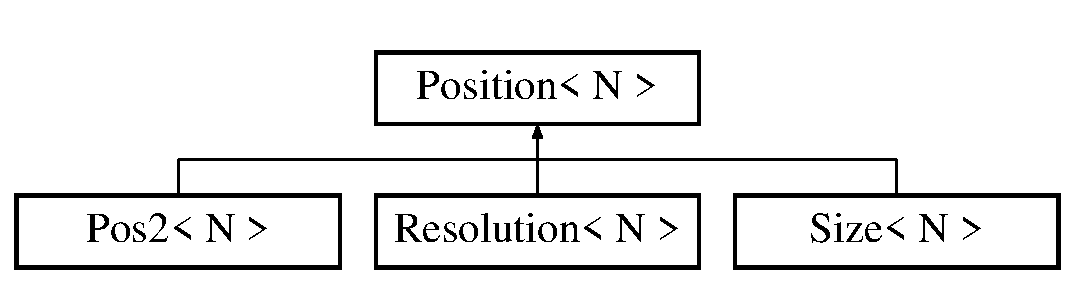
\includegraphics[height=2.000000cm]{struct_position}
\end{center}
\end{figure}
\subsection*{Public Member Functions}
\begin{DoxyCompactItemize}
\item 
\hyperlink{struct_position_ae3a67f3e6f27a5594c181ca55d2b2ef3}{Position} ()
\item 
\hyperlink{struct_position_a82e58f222f30e32c322d77bf9a20352b}{Position} (const \hyperlink{struct_bounds_check}{Bounds\-Check}$<$ N $>$ \&check)
\item 
\hyperlink{struct_position_a01b903d664fb8ac74a9342116ce63287}{Position} (N n)
\item 
\hyperlink{struct_position_a14a1831fd5c139aef062778edc05397d}{Position} (N n, const \hyperlink{struct_bounds_check}{Bounds\-Check}$<$ N $>$ \&check)
\item 
{\footnotesize template$<$typename R $>$ }\\\hyperlink{struct_position_a5f4ebf0205cb9e52e6f78784ca34d733}{Position} (\hyperlink{class_fast_rand}{Fast\-Rand}$<$ R $>$ rand)
\item 
{\footnotesize template$<$typename R $>$ }\\\hyperlink{struct_position_aa7e02fe8aeff4147c31184d981813f9d}{Position} (\hyperlink{class_fast_rand}{Fast\-Rand}$<$ R $>$ rand, const \hyperlink{struct_bounds_check}{Bounds\-Check}$<$ N $>$ \&check)
\item 
\hyperlink{struct_position_a7b49db88251912bf531acec16719eb98}{Position} (const \hyperlink{struct_position}{Position} \&other)
\item 
\hyperlink{struct_position_adfe6dffd68cbf7f26945bfb1a307fa6c}{Position} (const \hyperlink{struct_position}{Position} \&other, const \hyperlink{struct_bounds_check}{Bounds\-Check}$<$ N $>$ \&check)
\item 
\hyperlink{struct_position_a370b6460b790eef270233cd7a3527721}{Position} (\hyperlink{struct_position}{Position} \&\&other)
\item 
\hyperlink{struct_position_a1072383b9a22b17759b55f897986f011}{Position} (\hyperlink{struct_position}{Position} \&\&other, const \hyperlink{struct_bounds_check}{Bounds\-Check}$<$ N $>$ \&check)
\item 
\hyperlink{struct_position_a410251ddeee4121896cac284e3d63de2}{Position} (N \hyperlink{struct_position_af908be922fc88d89d81be7d08d06f761}{x}, N \hyperlink{struct_position_af434f54a0aad8bbfc3806ebdd197aa3b}{y}, N \hyperlink{struct_position_ac430da98504c2d4fd685c0363d728474}{z})
\item 
\hyperlink{struct_position_ae82fce224d7ef1599321a94b0a6f0cee}{Position} (N \hyperlink{struct_position_af908be922fc88d89d81be7d08d06f761}{x}, N \hyperlink{struct_position_af434f54a0aad8bbfc3806ebdd197aa3b}{y}, N \hyperlink{struct_position_ac430da98504c2d4fd685c0363d728474}{z}, const \hyperlink{struct_bounds_check}{Bounds\-Check}$<$ N $>$ \&check)
\item 
virtual \hyperlink{struct_position_a21a4e620b847f606fe2e1c5244f0f78e}{$\sim$\-Position} ()
\item 
virtual \hyperlink{struct_position}{Position} \& \hyperlink{struct_position_a669073574ecd196d45ea9d2ff0e3cced}{operator=} (const \hyperlink{struct_position}{Position} \&rhs)
\item 
virtual \hyperlink{struct_position}{Position} \& \hyperlink{struct_position_a580451251fc288d806524683fc85550a}{operator=} (\hyperlink{struct_position}{Position} \&\&rhs)
\item 
virtual bool \hyperlink{struct_position_ac895fed24f992ab43913207bd5fb7048}{operator==} (const \hyperlink{struct_position}{Position} \&rhs) const 
\item 
virtual bool \hyperlink{struct_position_a41b600238d7f4b174ed2c7dcd1ff8214}{operator==} (\hyperlink{struct_position}{Position} \&rhs) const 
\item 
virtual bool \hyperlink{struct_position_a4be02284917613eaa574c3ebbbbbfcb8}{operator!=} (const \hyperlink{struct_position}{Position} \&rhs) const 
\item 
virtual bool \hyperlink{struct_position_acaf1ee869c4bee9e4a6b152eee96efda}{operator!=} (\hyperlink{struct_position}{Position} \&rhs)
\item 
\hyperlink{struct_position}{Position} \hyperlink{struct_position_acee225b72b18e2468a8015fe3585958e}{operator+} (const \hyperlink{struct_position}{Position} \&rhs) const 
\item 
\hyperlink{struct_position}{Position} \hyperlink{struct_position_adc25e016e77688fabb733febd70dc3da}{operator-\/} (const \hyperlink{struct_position}{Position} \&rhs) const 
\item 
\hyperlink{struct_position}{Position} \hyperlink{struct_position_a95f98be024d028f87681c12092afcb28}{operator$\ast$} (const N n) const 
\item 
\hyperlink{struct_position}{Position} \hyperlink{struct_position_a51bc2b1d3ba86057fc8605208d2fb4cf}{operator/} (const N n) const 
\item 
virtual void \hyperlink{struct_position_af6cf3e9c2a535e8d988739e075ca76c1}{set\-All} (const N \hyperlink{struct_position_af908be922fc88d89d81be7d08d06f761}{x}, const N \hyperlink{struct_position_af434f54a0aad8bbfc3806ebdd197aa3b}{y}, const N \hyperlink{struct_position_ac430da98504c2d4fd685c0363d728474}{z})
\item 
virtual void \hyperlink{struct_position_abecde70eb2df3f274e171a06386feb4c}{set\-All} (const N \hyperlink{struct_position_af908be922fc88d89d81be7d08d06f761}{x}, const N \hyperlink{struct_position_af434f54a0aad8bbfc3806ebdd197aa3b}{y}, const N \hyperlink{struct_position_ac430da98504c2d4fd685c0363d728474}{z}, const \hyperlink{struct_bounds_check}{Bounds\-Check}$<$ N $>$ \&check)
\item 
virtual void \hyperlink{struct_position_a03ff8fcf39be2dc2ac547b9849a03fd6}{set\-All} (const \hyperlink{struct_position}{Position}$<$ N $>$ \&other)
\item 
virtual void \hyperlink{struct_position_ae7ad6637ca006d95867059c5405c2fdc}{set\-All} (const \hyperlink{struct_position}{Position}$<$ N $>$ \&other, const \hyperlink{struct_bounds_check}{Bounds\-Check}$<$ N $>$ \&check)
\item 
virtual void \hyperlink{struct_position_a90a919f4e1d7cdd0fcc50101d4c9dbd0}{set\-All} (const N n)
\item 
virtual void \hyperlink{struct_position_ae27c3958d1827450e434a8b2bb4d1092}{set\-All} (const N n, const \hyperlink{struct_bounds_check}{Bounds\-Check}$<$ N $>$ \&check)
\item 
virtual void \hyperlink{struct_position_ad625d6ef1db5f72883c6e2834f7cae81}{set\-All\-Zero} ()
\item 
N \hyperlink{struct_position_a7d1262a6b6f63f04c605bebf93a1f068}{get\-X} () const 
\item 
N \hyperlink{struct_position_a71d93e9a234bc4f32a61781c4e88bc10}{get\-Y} () const 
\item 
N \hyperlink{struct_position_a1d1171c9049c9a24be31bdb40e8662c0}{get\-Z} () const 
\item 
int \hyperlink{struct_position_a7c5b646e881251041b2373b0b9ee235b}{get\-Int\-X} () const 
\item 
int \hyperlink{struct_position_a2ddf4656749e96c1ad4bfec272521364}{get\-Int\-Y} () const 
\item 
int \hyperlink{struct_position_a41e19d862bf29d4aef2e25fbdd58f6b2}{get\-Int\-Z} () const 
\item 
virtual void \hyperlink{struct_position_a8ff94b86d9853ec1323129e2864a2f8d}{set\-X} (const N \hyperlink{struct_position_af908be922fc88d89d81be7d08d06f761}{x})
\item 
virtual void \hyperlink{struct_position_af1ca6db4823de1c43f874e72ce2b9b66}{set\-X} (const N \hyperlink{struct_position_af908be922fc88d89d81be7d08d06f761}{x}, const \hyperlink{struct_bounds_check}{Bounds\-Check}$<$ N $>$ \&check)
\item 
virtual void \hyperlink{struct_position_ab816c27eddb9c5d4951edfbb78dc7233}{set\-Y} (const N \hyperlink{struct_position_af434f54a0aad8bbfc3806ebdd197aa3b}{y})
\item 
virtual void \hyperlink{struct_position_a45f946eeadc660099a5c38f882e9074e}{set\-Y} (const N \hyperlink{struct_position_af434f54a0aad8bbfc3806ebdd197aa3b}{y}, const \hyperlink{struct_bounds_check}{Bounds\-Check}$<$ N $>$ \&check)
\item 
virtual void \hyperlink{struct_position_aa2c5e74e13456b840ce39ae8fc09c59b}{set\-Z} (const N \hyperlink{struct_position_ac430da98504c2d4fd685c0363d728474}{z})
\item 
virtual void \hyperlink{struct_position_ac3dd191a672bd9696e6bb2ccf3a622e2}{set\-Z} (const N \hyperlink{struct_position_ac430da98504c2d4fd685c0363d728474}{z}, const \hyperlink{struct_bounds_check}{Bounds\-Check}$<$ N $>$ \&check)
\item 
virtual void \hyperlink{struct_position_aca2bf935dd53d012fe3529b81a111e23}{x\-\_\-plus\-\_\-one} ()
\item 
virtual void \hyperlink{struct_position_a86f84c270f732ee8a285f0d8672529ad}{x\-\_\-plus\-\_\-one} (const \hyperlink{struct_bounds_check}{Bounds\-Check}$<$ N $>$ \&check)
\item 
virtual void \hyperlink{struct_position_aa5715ebd88d355988b0c0cf03814a271}{x\-\_\-minus\-\_\-one} ()
\item 
virtual void \hyperlink{struct_position_ab96af6ce73be6d52132f4d4e5bf77485}{x\-\_\-minus\-\_\-one} (const \hyperlink{struct_bounds_check}{Bounds\-Check}$<$ N $>$ \&check)
\item 
virtual void \hyperlink{struct_position_a9d1ef5169f798099ab268f62c5acc9e1}{y\-\_\-plus\-\_\-one} ()
\item 
virtual void \hyperlink{struct_position_a4ac4b6f9dc9ab06e64ce7b16c5dcdfaa}{y\-\_\-plus\-\_\-one} (const \hyperlink{struct_bounds_check}{Bounds\-Check}$<$ N $>$ \&check)
\item 
virtual void \hyperlink{struct_position_a9979106cd4c31b19ecbb831a91ec218a}{y\-\_\-minus\-\_\-one} ()
\item 
virtual void \hyperlink{struct_position_a0c0ff46cc0329a0e0109084fb1856233}{y\-\_\-minus\-\_\-one} (const \hyperlink{struct_bounds_check}{Bounds\-Check}$<$ N $>$ \&check)
\item 
virtual void \hyperlink{struct_position_a71640a61fe271ddc9e2451037a11a86d}{modify} (N delta\-\_\-x, N delta\-\_\-y, N delta\-\_\-z)
\item 
virtual void \hyperlink{struct_position_aa3e6b4d0e63e42c91332ffba79359252}{modify} (N delta\-\_\-x, N delta\-\_\-y, N delta\-\_\-z, const \hyperlink{struct_bounds_check}{Bounds\-Check}$<$ N $>$ \&check)
\item 
virtual void \hyperlink{struct_position_a81dd41480a91a0817c1937afef4cb644}{move\-Here} (N \hyperlink{struct_position_af908be922fc88d89d81be7d08d06f761}{x}, N \hyperlink{struct_position_af434f54a0aad8bbfc3806ebdd197aa3b}{y}, N \hyperlink{struct_position_ac430da98504c2d4fd685c0363d728474}{z})
\item 
virtual void \hyperlink{struct_position_a4fa2e78d31d34daba2d555394c4e4b80}{move\-Here} (N \hyperlink{struct_position_af908be922fc88d89d81be7d08d06f761}{x}, N \hyperlink{struct_position_af434f54a0aad8bbfc3806ebdd197aa3b}{y}, N \hyperlink{struct_position_ac430da98504c2d4fd685c0363d728474}{z}, const \hyperlink{struct_bounds_check}{Bounds\-Check}$<$ N $>$ \&check)
\item 
virtual void \hyperlink{struct_position_a3840e7e0c17531cd254810fe62340f52}{move\-Here} (const \hyperlink{struct_position}{Position}$<$ N $>$ \&other)
\item 
virtual void \hyperlink{struct_position_aa268c21ec09dbe0b579b0854ef74ddb9}{move\-Here} (const \hyperlink{struct_position}{Position}$<$ N $>$ \&other, const \hyperlink{struct_bounds_check}{Bounds\-Check}$<$ N $>$ \&check)
\item 
std\-::string \hyperlink{struct_position_a4ebba65bc16bffa822c653522c5d7dcb}{to\-String} () const 
\item 
void \hyperlink{struct_position_afd2bfedb3b315412862103233665fc02}{check\-Bounds} (const \hyperlink{struct_bounds_check}{Bounds\-Check}$<$ N $>$ $\ast$check, N obj\-Width=0, N obj\-Height=0)
\item 
void \hyperlink{struct_position_aaf90e9e75b999bf2c43064feaa3694eb}{check\-Bounds} (const \hyperlink{struct_bounds_check}{Bounds\-Check}$<$ N $>$ \&check, N obj\-Width=0, N obj\-Height=0)
\item 
bool \hyperlink{struct_position_aac17c8dcac3808518f5e13c7ecf31c19}{over\-Bounds} (const \hyperlink{struct_bounds_check}{Bounds\-Check}$<$ N $>$ $\ast$check, N obj\-Width=0, N obj\-Height=0) const 
\item 
bool \hyperlink{struct_position_a06da33376bc3a116664f8a34e816ba95}{over\-X\-Bounds} (const \hyperlink{struct_bounds_check}{Bounds\-Check}$<$ N $>$ $\ast$check) const 
\item 
bool \hyperlink{struct_position_a45f215fed381839bf860752780a9660f}{over\-Y\-Bounds} (const \hyperlink{struct_bounds_check}{Bounds\-Check}$<$ N $>$ $\ast$check) const 
\end{DoxyCompactItemize}
\subsection*{Static Public Member Functions}
\begin{DoxyCompactItemize}
\item 
static N \hyperlink{struct_position_acbec1420f0dc8f505c745b399ae93234}{calc\-Distance} (const \hyperlink{struct_position}{Position} \&here, const \hyperlink{struct_position}{Position} \&there)
\end{DoxyCompactItemize}
\subsection*{Protected Attributes}
\begin{DoxyCompactItemize}
\item 
N \hyperlink{struct_position_af908be922fc88d89d81be7d08d06f761}{x}
\item 
N \hyperlink{struct_position_af434f54a0aad8bbfc3806ebdd197aa3b}{y}
\item 
N \hyperlink{struct_position_ac430da98504c2d4fd685c0363d728474}{z}
\end{DoxyCompactItemize}
\subsection*{Friends}
\begin{DoxyCompactItemize}
\item 
{\footnotesize template$<$typename O , typename P $>$ }\\const \hyperlink{struct_position}{Position}$<$ P $>$ $\ast$ \hyperlink{struct_position_aa839563739359a38d864a2d4a4e616e3}{operator+} (const \hyperlink{struct_position}{Position}$<$ P $>$ \&lhs, const \hyperlink{struct_position}{Position}$<$ O $>$ $\ast$rhs)
\item 
{\footnotesize template$<$typename O , typename P $>$ }\\const \hyperlink{struct_position}{Position}$<$ P $>$ $\ast$ \hyperlink{struct_position_a952651ce7dae93907c21bf178d58dd94}{operator-\/} (const \hyperlink{struct_position}{Position}$<$ P $>$ \&lhs, const \hyperlink{struct_position}{Position}$<$ O $>$ $\ast$rhs)
\item 
ostream \& \hyperlink{struct_position_a7adf840eaa5364c5fdddbc148fcbbdee}{operator$<$$<$} (std\-::ostream \&os, const \hyperlink{struct_position}{Position}$<$ N $>$ $\ast$pos)
\item 
ostream \& \hyperlink{struct_position_a8d4dbe2f6bca09c4129d69b47bc4b2ac}{operator$<$$<$} (std\-::ostream \&os, const \hyperlink{struct_position}{Position}$<$ N $>$ \&pos)
\end{DoxyCompactItemize}


\subsection{Detailed Description}
\subsubsection*{template$<$typename N$>$struct Position$<$ N $>$}

Position$<$$>$ is a simple vector type with the useful feature of storing all its previous states, back through time. Thus an object using \hyperlink{struct_position}{Position} to store location information will be able to retrace its steps. Note\-: Classes with a \hyperlink{struct_position}{Position} data member will typically want to have a pointer, instead of holding the \hyperlink{struct_position}{Position} locally. This is because many objects in the World may not actually have a physcical \hyperlink{struct_position}{Position} in space, in which case they can just hold a null pointer. 

Definition at line 63 of file Position.\-hpp.



\subsection{Constructor \& Destructor Documentation}
\hypertarget{struct_position_ae3a67f3e6f27a5594c181ca55d2b2ef3}{\index{Position@{Position}!Position@{Position}}
\index{Position@{Position}!Position@{Position}}
\subsubsection[{Position}]{\setlength{\rightskip}{0pt plus 5cm}template$<$typename N$>$ {\bf Position}$<$ N $>$\-::{\bf Position} (
\begin{DoxyParamCaption}
{}
\end{DoxyParamCaption}
)\hspace{0.3cm}{\ttfamily [inline]}}}\label{struct_position_ae3a67f3e6f27a5594c181ca55d2b2ef3}
Creates a Positionwith all coordinates initialized to 0 

Definition at line 75 of file Position.\-hpp.

\hypertarget{struct_position_a82e58f222f30e32c322d77bf9a20352b}{\index{Position@{Position}!Position@{Position}}
\index{Position@{Position}!Position@{Position}}
\subsubsection[{Position}]{\setlength{\rightskip}{0pt plus 5cm}template$<$typename N$>$ {\bf Position}$<$ N $>$\-::{\bf Position} (
\begin{DoxyParamCaption}
\item[{const {\bf Bounds\-Check}$<$ N $>$ \&}]{check}
\end{DoxyParamCaption}
)\hspace{0.3cm}{\ttfamily [inline]}}}\label{struct_position_a82e58f222f30e32c322d77bf9a20352b}
Creates a Positionwith all coordinates initialized to 0 

Definition at line 80 of file Position.\-hpp.

\hypertarget{struct_position_a01b903d664fb8ac74a9342116ce63287}{\index{Position@{Position}!Position@{Position}}
\index{Position@{Position}!Position@{Position}}
\subsubsection[{Position}]{\setlength{\rightskip}{0pt plus 5cm}template$<$typename N$>$ {\bf Position}$<$ N $>$\-::{\bf Position} (
\begin{DoxyParamCaption}
\item[{N}]{n}
\end{DoxyParamCaption}
)\hspace{0.3cm}{\ttfamily [inline]}}}\label{struct_position_a01b903d664fb8ac74a9342116ce63287}
Creates a Positionwith all coordinates initialized to n 

Definition at line 85 of file Position.\-hpp.

\hypertarget{struct_position_a14a1831fd5c139aef062778edc05397d}{\index{Position@{Position}!Position@{Position}}
\index{Position@{Position}!Position@{Position}}
\subsubsection[{Position}]{\setlength{\rightskip}{0pt plus 5cm}template$<$typename N$>$ {\bf Position}$<$ N $>$\-::{\bf Position} (
\begin{DoxyParamCaption}
\item[{N}]{n, }
\item[{const {\bf Bounds\-Check}$<$ N $>$ \&}]{check}
\end{DoxyParamCaption}
)\hspace{0.3cm}{\ttfamily [inline]}}}\label{struct_position_a14a1831fd5c139aef062778edc05397d}
Creates a Positionwith all coordinates initialized to n 

Definition at line 90 of file Position.\-hpp.

\hypertarget{struct_position_a5f4ebf0205cb9e52e6f78784ca34d733}{\index{Position@{Position}!Position@{Position}}
\index{Position@{Position}!Position@{Position}}
\subsubsection[{Position}]{\setlength{\rightskip}{0pt plus 5cm}template$<$typename N$>$ template$<$typename R $>$ {\bf Position}$<$ N $>$\-::{\bf Position} (
\begin{DoxyParamCaption}
\item[{{\bf Fast\-Rand}$<$ R $>$}]{rand}
\end{DoxyParamCaption}
)\hspace{0.3cm}{\ttfamily [inline]}}}\label{struct_position_a5f4ebf0205cb9e52e6f78784ca34d733}
Creates a Positionwith all coordinates randomized, with bounds set by check 

Definition at line 96 of file Position.\-hpp.

\hypertarget{struct_position_aa7e02fe8aeff4147c31184d981813f9d}{\index{Position@{Position}!Position@{Position}}
\index{Position@{Position}!Position@{Position}}
\subsubsection[{Position}]{\setlength{\rightskip}{0pt plus 5cm}template$<$typename N$>$ template$<$typename R $>$ {\bf Position}$<$ N $>$\-::{\bf Position} (
\begin{DoxyParamCaption}
\item[{{\bf Fast\-Rand}$<$ R $>$}]{rand, }
\item[{const {\bf Bounds\-Check}$<$ N $>$ \&}]{check}
\end{DoxyParamCaption}
)\hspace{0.3cm}{\ttfamily [inline]}}}\label{struct_position_aa7e02fe8aeff4147c31184d981813f9d}
Creates a Positionwith all coordinates randomized, with bounds set by check 

Definition at line 105 of file Position.\-hpp.

\hypertarget{struct_position_a7b49db88251912bf531acec16719eb98}{\index{Position@{Position}!Position@{Position}}
\index{Position@{Position}!Position@{Position}}
\subsubsection[{Position}]{\setlength{\rightskip}{0pt plus 5cm}template$<$typename N$>$ {\bf Position}$<$ N $>$\-::{\bf Position} (
\begin{DoxyParamCaption}
\item[{const {\bf Position}$<$ N $>$ \&}]{other}
\end{DoxyParamCaption}
)\hspace{0.3cm}{\ttfamily [inline]}}}\label{struct_position_a7b49db88251912bf531acec16719eb98}
Copy constructor for \hyperlink{struct_position}{Position} 

Definition at line 116 of file Position.\-hpp.

\hypertarget{struct_position_adfe6dffd68cbf7f26945bfb1a307fa6c}{\index{Position@{Position}!Position@{Position}}
\index{Position@{Position}!Position@{Position}}
\subsubsection[{Position}]{\setlength{\rightskip}{0pt plus 5cm}template$<$typename N$>$ {\bf Position}$<$ N $>$\-::{\bf Position} (
\begin{DoxyParamCaption}
\item[{const {\bf Position}$<$ N $>$ \&}]{other, }
\item[{const {\bf Bounds\-Check}$<$ N $>$ \&}]{check}
\end{DoxyParamCaption}
)\hspace{0.3cm}{\ttfamily [inline]}}}\label{struct_position_adfe6dffd68cbf7f26945bfb1a307fa6c}
Copy constructor for \hyperlink{struct_position}{Position} 

Definition at line 121 of file Position.\-hpp.

\hypertarget{struct_position_a370b6460b790eef270233cd7a3527721}{\index{Position@{Position}!Position@{Position}}
\index{Position@{Position}!Position@{Position}}
\subsubsection[{Position}]{\setlength{\rightskip}{0pt plus 5cm}template$<$typename N$>$ {\bf Position}$<$ N $>$\-::{\bf Position} (
\begin{DoxyParamCaption}
\item[{{\bf Position}$<$ N $>$ \&\&}]{other}
\end{DoxyParamCaption}
)\hspace{0.3cm}{\ttfamily [inline]}}}\label{struct_position_a370b6460b790eef270233cd7a3527721}
Move constructor for \hyperlink{struct_position}{Position} 

Definition at line 128 of file Position.\-hpp.

\hypertarget{struct_position_a1072383b9a22b17759b55f897986f011}{\index{Position@{Position}!Position@{Position}}
\index{Position@{Position}!Position@{Position}}
\subsubsection[{Position}]{\setlength{\rightskip}{0pt plus 5cm}template$<$typename N$>$ {\bf Position}$<$ N $>$\-::{\bf Position} (
\begin{DoxyParamCaption}
\item[{{\bf Position}$<$ N $>$ \&\&}]{other, }
\item[{const {\bf Bounds\-Check}$<$ N $>$ \&}]{check}
\end{DoxyParamCaption}
)\hspace{0.3cm}{\ttfamily [inline]}}}\label{struct_position_a1072383b9a22b17759b55f897986f011}
Move constructor for \hyperlink{struct_position}{Position} 

Definition at line 133 of file Position.\-hpp.

\hypertarget{struct_position_a410251ddeee4121896cac284e3d63de2}{\index{Position@{Position}!Position@{Position}}
\index{Position@{Position}!Position@{Position}}
\subsubsection[{Position}]{\setlength{\rightskip}{0pt plus 5cm}template$<$typename N$>$ {\bf Position}$<$ N $>$\-::{\bf Position} (
\begin{DoxyParamCaption}
\item[{N}]{x, }
\item[{N}]{y, }
\item[{N}]{z}
\end{DoxyParamCaption}
)\hspace{0.3cm}{\ttfamily [inline]}}}\label{struct_position_a410251ddeee4121896cac284e3d63de2}
Creates a \hyperlink{struct_position}{Position} with coordinates initialized to the given arguments


\begin{DoxyParams}{Parameters}
{\em x} & The x coordinate \\
\hline
{\em y} & The y coordinate \\
\hline
{\em z} & The z coordinate \\
\hline
\end{DoxyParams}


Definition at line 145 of file Position.\-hpp.

\hypertarget{struct_position_ae82fce224d7ef1599321a94b0a6f0cee}{\index{Position@{Position}!Position@{Position}}
\index{Position@{Position}!Position@{Position}}
\subsubsection[{Position}]{\setlength{\rightskip}{0pt plus 5cm}template$<$typename N$>$ {\bf Position}$<$ N $>$\-::{\bf Position} (
\begin{DoxyParamCaption}
\item[{N}]{x, }
\item[{N}]{y, }
\item[{N}]{z, }
\item[{const {\bf Bounds\-Check}$<$ N $>$ \&}]{check}
\end{DoxyParamCaption}
)\hspace{0.3cm}{\ttfamily [inline]}}}\label{struct_position_ae82fce224d7ef1599321a94b0a6f0cee}
Creates a \hyperlink{struct_position}{Position} with coordinates initialized to the given arguments


\begin{DoxyParams}{Parameters}
{\em x} & The x coordinate \\
\hline
{\em y} & The y coordinate \\
\hline
{\em z} & The z coordinate \\
\hline
\end{DoxyParams}


Definition at line 155 of file Position.\-hpp.

\hypertarget{struct_position_a21a4e620b847f606fe2e1c5244f0f78e}{\index{Position@{Position}!$\sim$\-Position@{$\sim$\-Position}}
\index{$\sim$\-Position@{$\sim$\-Position}!Position@{Position}}
\subsubsection[{$\sim$\-Position}]{\setlength{\rightskip}{0pt plus 5cm}template$<$typename N$>$ virtual {\bf Position}$<$ N $>$\-::$\sim${\bf Position} (
\begin{DoxyParamCaption}
{}
\end{DoxyParamCaption}
)\hspace{0.3cm}{\ttfamily [inline]}, {\ttfamily [virtual]}}}\label{struct_position_a21a4e620b847f606fe2e1c5244f0f78e}
Destructor for \hyperlink{struct_position}{Position} 

Definition at line 162 of file Position.\-hpp.



\subsection{Member Function Documentation}
\hypertarget{struct_position_acbec1420f0dc8f505c745b399ae93234}{\index{Position@{Position}!calc\-Distance@{calc\-Distance}}
\index{calc\-Distance@{calc\-Distance}!Position@{Position}}
\subsubsection[{calc\-Distance}]{\setlength{\rightskip}{0pt plus 5cm}template$<$typename N$>$ static N {\bf Position}$<$ N $>$\-::calc\-Distance (
\begin{DoxyParamCaption}
\item[{const {\bf Position}$<$ N $>$ \&}]{here, }
\item[{const {\bf Position}$<$ N $>$ \&}]{there}
\end{DoxyParamCaption}
)\hspace{0.3cm}{\ttfamily [inline]}, {\ttfamily [static]}}}\label{struct_position_acbec1420f0dc8f505c745b399ae93234}


Definition at line 435 of file Position.\-hpp.

\hypertarget{struct_position_afd2bfedb3b315412862103233665fc02}{\index{Position@{Position}!check\-Bounds@{check\-Bounds}}
\index{check\-Bounds@{check\-Bounds}!Position@{Position}}
\subsubsection[{check\-Bounds}]{\setlength{\rightskip}{0pt plus 5cm}template$<$typename N$>$ void {\bf Position}$<$ N $>$\-::check\-Bounds (
\begin{DoxyParamCaption}
\item[{const {\bf Bounds\-Check}$<$ N $>$ $\ast$}]{check, }
\item[{N}]{obj\-Width = {\ttfamily 0}, }
\item[{N}]{obj\-Height = {\ttfamily 0}}
\end{DoxyParamCaption}
)\hspace{0.3cm}{\ttfamily [inline]}}}\label{struct_position_afd2bfedb3b315412862103233665fc02}


Definition at line 451 of file Position.\-hpp.

\hypertarget{struct_position_aaf90e9e75b999bf2c43064feaa3694eb}{\index{Position@{Position}!check\-Bounds@{check\-Bounds}}
\index{check\-Bounds@{check\-Bounds}!Position@{Position}}
\subsubsection[{check\-Bounds}]{\setlength{\rightskip}{0pt plus 5cm}template$<$typename N$>$ void {\bf Position}$<$ N $>$\-::check\-Bounds (
\begin{DoxyParamCaption}
\item[{const {\bf Bounds\-Check}$<$ N $>$ \&}]{check, }
\item[{N}]{obj\-Width = {\ttfamily 0}, }
\item[{N}]{obj\-Height = {\ttfamily 0}}
\end{DoxyParamCaption}
)\hspace{0.3cm}{\ttfamily [inline]}}}\label{struct_position_aaf90e9e75b999bf2c43064feaa3694eb}


Definition at line 487 of file Position.\-hpp.

\hypertarget{struct_position_a7c5b646e881251041b2373b0b9ee235b}{\index{Position@{Position}!get\-Int\-X@{get\-Int\-X}}
\index{get\-Int\-X@{get\-Int\-X}!Position@{Position}}
\subsubsection[{get\-Int\-X}]{\setlength{\rightskip}{0pt plus 5cm}template$<$typename N$>$ int {\bf Position}$<$ N $>$\-::get\-Int\-X (
\begin{DoxyParamCaption}
{}
\end{DoxyParamCaption}
) const\hspace{0.3cm}{\ttfamily [inline]}}}\label{struct_position_a7c5b646e881251041b2373b0b9ee235b}
\begin{DoxyReturn}{Returns}
x as an integer 
\end{DoxyReturn}


Definition at line 332 of file Position.\-hpp.

\hypertarget{struct_position_a2ddf4656749e96c1ad4bfec272521364}{\index{Position@{Position}!get\-Int\-Y@{get\-Int\-Y}}
\index{get\-Int\-Y@{get\-Int\-Y}!Position@{Position}}
\subsubsection[{get\-Int\-Y}]{\setlength{\rightskip}{0pt plus 5cm}template$<$typename N$>$ int {\bf Position}$<$ N $>$\-::get\-Int\-Y (
\begin{DoxyParamCaption}
{}
\end{DoxyParamCaption}
) const\hspace{0.3cm}{\ttfamily [inline]}}}\label{struct_position_a2ddf4656749e96c1ad4bfec272521364}
\begin{DoxyReturn}{Returns}
z as an integer 
\end{DoxyReturn}


Definition at line 337 of file Position.\-hpp.

\hypertarget{struct_position_a41e19d862bf29d4aef2e25fbdd58f6b2}{\index{Position@{Position}!get\-Int\-Z@{get\-Int\-Z}}
\index{get\-Int\-Z@{get\-Int\-Z}!Position@{Position}}
\subsubsection[{get\-Int\-Z}]{\setlength{\rightskip}{0pt plus 5cm}template$<$typename N$>$ int {\bf Position}$<$ N $>$\-::get\-Int\-Z (
\begin{DoxyParamCaption}
{}
\end{DoxyParamCaption}
) const\hspace{0.3cm}{\ttfamily [inline]}}}\label{struct_position_a41e19d862bf29d4aef2e25fbdd58f6b2}
\begin{DoxyReturn}{Returns}
z as an integer 
\end{DoxyReturn}


Definition at line 342 of file Position.\-hpp.

\hypertarget{struct_position_a7d1262a6b6f63f04c605bebf93a1f068}{\index{Position@{Position}!get\-X@{get\-X}}
\index{get\-X@{get\-X}!Position@{Position}}
\subsubsection[{get\-X}]{\setlength{\rightskip}{0pt plus 5cm}template$<$typename N$>$ N {\bf Position}$<$ N $>$\-::get\-X (
\begin{DoxyParamCaption}
{}
\end{DoxyParamCaption}
) const\hspace{0.3cm}{\ttfamily [inline]}}}\label{struct_position_a7d1262a6b6f63f04c605bebf93a1f068}


Definition at line 323 of file Position.\-hpp.

\hypertarget{struct_position_a71d93e9a234bc4f32a61781c4e88bc10}{\index{Position@{Position}!get\-Y@{get\-Y}}
\index{get\-Y@{get\-Y}!Position@{Position}}
\subsubsection[{get\-Y}]{\setlength{\rightskip}{0pt plus 5cm}template$<$typename N$>$ N {\bf Position}$<$ N $>$\-::get\-Y (
\begin{DoxyParamCaption}
{}
\end{DoxyParamCaption}
) const\hspace{0.3cm}{\ttfamily [inline]}}}\label{struct_position_a71d93e9a234bc4f32a61781c4e88bc10}


Definition at line 325 of file Position.\-hpp.

\hypertarget{struct_position_a1d1171c9049c9a24be31bdb40e8662c0}{\index{Position@{Position}!get\-Z@{get\-Z}}
\index{get\-Z@{get\-Z}!Position@{Position}}
\subsubsection[{get\-Z}]{\setlength{\rightskip}{0pt plus 5cm}template$<$typename N$>$ N {\bf Position}$<$ N $>$\-::get\-Z (
\begin{DoxyParamCaption}
{}
\end{DoxyParamCaption}
) const\hspace{0.3cm}{\ttfamily [inline]}}}\label{struct_position_a1d1171c9049c9a24be31bdb40e8662c0}


Definition at line 327 of file Position.\-hpp.

\hypertarget{struct_position_a71640a61fe271ddc9e2451037a11a86d}{\index{Position@{Position}!modify@{modify}}
\index{modify@{modify}!Position@{Position}}
\subsubsection[{modify}]{\setlength{\rightskip}{0pt plus 5cm}template$<$typename N$>$ virtual void {\bf Position}$<$ N $>$\-::modify (
\begin{DoxyParamCaption}
\item[{N}]{delta\-\_\-x, }
\item[{N}]{delta\-\_\-y, }
\item[{N}]{delta\-\_\-z}
\end{DoxyParamCaption}
)\hspace{0.3cm}{\ttfamily [inline]}, {\ttfamily [virtual]}}}\label{struct_position_a71640a61fe271ddc9e2451037a11a86d}
Increments or decrements the x, y and z values according to the arguments passed in. Use negative values to decrement. Passing 0 for any argument will keep the x, y, or z value the same.


\begin{DoxyParams}{Parameters}
{\em delta\-\_\-x} & The change in x value \\
\hline
{\em delta\-\_\-y} & The change in y value \\
\hline
{\em delta\-\_\-z} & The change in z value \\
\hline
\end{DoxyParams}


Reimplemented in \hyperlink{struct_pos2_a3065dacbd8e42b36fd5af0775a9342d8}{Pos2$<$ N $>$}, and \hyperlink{struct_pos2_a3065dacbd8e42b36fd5af0775a9342d8}{Pos2$<$ float $>$}.



Definition at line 384 of file Position.\-hpp.

\hypertarget{struct_position_aa3e6b4d0e63e42c91332ffba79359252}{\index{Position@{Position}!modify@{modify}}
\index{modify@{modify}!Position@{Position}}
\subsubsection[{modify}]{\setlength{\rightskip}{0pt plus 5cm}template$<$typename N$>$ virtual void {\bf Position}$<$ N $>$\-::modify (
\begin{DoxyParamCaption}
\item[{N}]{delta\-\_\-x, }
\item[{N}]{delta\-\_\-y, }
\item[{N}]{delta\-\_\-z, }
\item[{const {\bf Bounds\-Check}$<$ N $>$ \&}]{check}
\end{DoxyParamCaption}
)\hspace{0.3cm}{\ttfamily [inline]}, {\ttfamily [virtual]}}}\label{struct_position_aa3e6b4d0e63e42c91332ffba79359252}
Increments or decrements the x, y and z values according to the arguments passed in. Use negative values to decrement. Passing 0 for any argument will keep the x, y, or z value the same.


\begin{DoxyParams}{Parameters}
{\em delta\-\_\-x} & The change in x value \\
\hline
{\em delta\-\_\-y} & The change in y value \\
\hline
{\em delta\-\_\-z} & The change in z value \\
\hline
\end{DoxyParams}


Reimplemented in \hyperlink{struct_pos2_ab0ddc65822cce3935319977f3ab7c8e2}{Pos2$<$ N $>$}, and \hyperlink{struct_pos2_ab0ddc65822cce3935319977f3ab7c8e2}{Pos2$<$ float $>$}.



Definition at line 405 of file Position.\-hpp.

\hypertarget{struct_position_a81dd41480a91a0817c1937afef4cb644}{\index{Position@{Position}!move\-Here@{move\-Here}}
\index{move\-Here@{move\-Here}!Position@{Position}}
\subsubsection[{move\-Here}]{\setlength{\rightskip}{0pt plus 5cm}template$<$typename N$>$ virtual void {\bf Position}$<$ N $>$\-::move\-Here (
\begin{DoxyParamCaption}
\item[{N}]{x, }
\item[{N}]{y, }
\item[{N}]{z}
\end{DoxyParamCaption}
)\hspace{0.3cm}{\ttfamily [inline]}, {\ttfamily [virtual]}}}\label{struct_position_a81dd41480a91a0817c1937afef4cb644}


Reimplemented in \hyperlink{struct_pos2_a8cb8d4f4d076ef9ecbb34bcb351ba8fa}{Pos2$<$ N $>$}, and \hyperlink{struct_pos2_a8cb8d4f4d076ef9ecbb34bcb351ba8fa}{Pos2$<$ float $>$}.



Definition at line 417 of file Position.\-hpp.

\hypertarget{struct_position_a4fa2e78d31d34daba2d555394c4e4b80}{\index{Position@{Position}!move\-Here@{move\-Here}}
\index{move\-Here@{move\-Here}!Position@{Position}}
\subsubsection[{move\-Here}]{\setlength{\rightskip}{0pt plus 5cm}template$<$typename N$>$ virtual void {\bf Position}$<$ N $>$\-::move\-Here (
\begin{DoxyParamCaption}
\item[{N}]{x, }
\item[{N}]{y, }
\item[{N}]{z, }
\item[{const {\bf Bounds\-Check}$<$ N $>$ \&}]{check}
\end{DoxyParamCaption}
)\hspace{0.3cm}{\ttfamily [inline]}, {\ttfamily [virtual]}}}\label{struct_position_a4fa2e78d31d34daba2d555394c4e4b80}


Reimplemented in \hyperlink{struct_pos2_a2cf33b5575ca6cd5a02dbc92ee22fe7a}{Pos2$<$ N $>$}, and \hyperlink{struct_pos2_a2cf33b5575ca6cd5a02dbc92ee22fe7a}{Pos2$<$ float $>$}.



Definition at line 421 of file Position.\-hpp.

\hypertarget{struct_position_a3840e7e0c17531cd254810fe62340f52}{\index{Position@{Position}!move\-Here@{move\-Here}}
\index{move\-Here@{move\-Here}!Position@{Position}}
\subsubsection[{move\-Here}]{\setlength{\rightskip}{0pt plus 5cm}template$<$typename N$>$ virtual void {\bf Position}$<$ N $>$\-::move\-Here (
\begin{DoxyParamCaption}
\item[{const {\bf Position}$<$ N $>$ \&}]{other}
\end{DoxyParamCaption}
)\hspace{0.3cm}{\ttfamily [inline]}, {\ttfamily [virtual]}}}\label{struct_position_a3840e7e0c17531cd254810fe62340f52}


Reimplemented in \hyperlink{struct_pos2_a112150629c1c77a913f401e8948849b0}{Pos2$<$ N $>$}, and \hyperlink{struct_pos2_a112150629c1c77a913f401e8948849b0}{Pos2$<$ float $>$}.



Definition at line 426 of file Position.\-hpp.

\hypertarget{struct_position_aa268c21ec09dbe0b579b0854ef74ddb9}{\index{Position@{Position}!move\-Here@{move\-Here}}
\index{move\-Here@{move\-Here}!Position@{Position}}
\subsubsection[{move\-Here}]{\setlength{\rightskip}{0pt plus 5cm}template$<$typename N$>$ virtual void {\bf Position}$<$ N $>$\-::move\-Here (
\begin{DoxyParamCaption}
\item[{const {\bf Position}$<$ N $>$ \&}]{other, }
\item[{const {\bf Bounds\-Check}$<$ N $>$ \&}]{check}
\end{DoxyParamCaption}
)\hspace{0.3cm}{\ttfamily [inline]}, {\ttfamily [virtual]}}}\label{struct_position_aa268c21ec09dbe0b579b0854ef74ddb9}


Reimplemented in \hyperlink{struct_pos2_aa743473a51150e91792af64c00153ed9}{Pos2$<$ N $>$}, and \hyperlink{struct_pos2_aa743473a51150e91792af64c00153ed9}{Pos2$<$ float $>$}.



Definition at line 430 of file Position.\-hpp.

\hypertarget{struct_position_a4be02284917613eaa574c3ebbbbbfcb8}{\index{Position@{Position}!operator!=@{operator!=}}
\index{operator!=@{operator!=}!Position@{Position}}
\subsubsection[{operator!=}]{\setlength{\rightskip}{0pt plus 5cm}template$<$typename N$>$ virtual bool {\bf Position}$<$ N $>$\-::operator!= (
\begin{DoxyParamCaption}
\item[{const {\bf Position}$<$ N $>$ \&}]{rhs}
\end{DoxyParamCaption}
) const\hspace{0.3cm}{\ttfamily [inline]}, {\ttfamily [virtual]}}}\label{struct_position_a4be02284917613eaa574c3ebbbbbfcb8}


Reimplemented in \hyperlink{struct_pos2_ae519d026266e7c63cede223ba78d68cf}{Pos2$<$ N $>$}.



Definition at line 210 of file Position.\-hpp.

\hypertarget{struct_position_acaf1ee869c4bee9e4a6b152eee96efda}{\index{Position@{Position}!operator!=@{operator!=}}
\index{operator!=@{operator!=}!Position@{Position}}
\subsubsection[{operator!=}]{\setlength{\rightskip}{0pt plus 5cm}template$<$typename N$>$ virtual bool {\bf Position}$<$ N $>$\-::operator!= (
\begin{DoxyParamCaption}
\item[{{\bf Position}$<$ N $>$ \&}]{rhs}
\end{DoxyParamCaption}
)\hspace{0.3cm}{\ttfamily [inline]}, {\ttfamily [virtual]}}}\label{struct_position_acaf1ee869c4bee9e4a6b152eee96efda}


Definition at line 214 of file Position.\-hpp.

\hypertarget{struct_position_a95f98be024d028f87681c12092afcb28}{\index{Position@{Position}!operator$\ast$@{operator$\ast$}}
\index{operator$\ast$@{operator$\ast$}!Position@{Position}}
\subsubsection[{operator$\ast$}]{\setlength{\rightskip}{0pt plus 5cm}template$<$typename N$>$ {\bf Position} {\bf Position}$<$ N $>$\-::operator$\ast$ (
\begin{DoxyParamCaption}
\item[{const N}]{n}
\end{DoxyParamCaption}
) const\hspace{0.3cm}{\ttfamily [inline]}}}\label{struct_position_a95f98be024d028f87681c12092afcb28}


Definition at line 240 of file Position.\-hpp.

\hypertarget{struct_position_acee225b72b18e2468a8015fe3585958e}{\index{Position@{Position}!operator+@{operator+}}
\index{operator+@{operator+}!Position@{Position}}
\subsubsection[{operator+}]{\setlength{\rightskip}{0pt plus 5cm}template$<$typename N$>$ {\bf Position} {\bf Position}$<$ N $>$\-::operator+ (
\begin{DoxyParamCaption}
\item[{const {\bf Position}$<$ N $>$ \&}]{rhs}
\end{DoxyParamCaption}
) const\hspace{0.3cm}{\ttfamily [inline]}}}\label{struct_position_acee225b72b18e2468a8015fe3585958e}


Definition at line 218 of file Position.\-hpp.

\hypertarget{struct_position_adc25e016e77688fabb733febd70dc3da}{\index{Position@{Position}!operator-\/@{operator-\/}}
\index{operator-\/@{operator-\/}!Position@{Position}}
\subsubsection[{operator-\/}]{\setlength{\rightskip}{0pt plus 5cm}template$<$typename N$>$ {\bf Position} {\bf Position}$<$ N $>$\-::operator-\/ (
\begin{DoxyParamCaption}
\item[{const {\bf Position}$<$ N $>$ \&}]{rhs}
\end{DoxyParamCaption}
) const\hspace{0.3cm}{\ttfamily [inline]}}}\label{struct_position_adc25e016e77688fabb733febd70dc3da}


Definition at line 229 of file Position.\-hpp.

\hypertarget{struct_position_a51bc2b1d3ba86057fc8605208d2fb4cf}{\index{Position@{Position}!operator/@{operator/}}
\index{operator/@{operator/}!Position@{Position}}
\subsubsection[{operator/}]{\setlength{\rightskip}{0pt plus 5cm}template$<$typename N$>$ {\bf Position} {\bf Position}$<$ N $>$\-::operator/ (
\begin{DoxyParamCaption}
\item[{const N}]{n}
\end{DoxyParamCaption}
) const\hspace{0.3cm}{\ttfamily [inline]}}}\label{struct_position_a51bc2b1d3ba86057fc8605208d2fb4cf}


Definition at line 251 of file Position.\-hpp.

\hypertarget{struct_position_a669073574ecd196d45ea9d2ff0e3cced}{\index{Position@{Position}!operator=@{operator=}}
\index{operator=@{operator=}!Position@{Position}}
\subsubsection[{operator=}]{\setlength{\rightskip}{0pt plus 5cm}template$<$typename N$>$ virtual {\bf Position}\& {\bf Position}$<$ N $>$\-::operator= (
\begin{DoxyParamCaption}
\item[{const {\bf Position}$<$ N $>$ \&}]{rhs}
\end{DoxyParamCaption}
)\hspace{0.3cm}{\ttfamily [inline]}, {\ttfamily [virtual]}}}\label{struct_position_a669073574ecd196d45ea9d2ff0e3cced}
Assigment operator (copy). 

Reimplemented in \hyperlink{struct_pos2_a340228a5c2933605e488596eed7fdc16}{Pos2$<$ N $>$}.



Definition at line 168 of file Position.\-hpp.

\hypertarget{struct_position_a580451251fc288d806524683fc85550a}{\index{Position@{Position}!operator=@{operator=}}
\index{operator=@{operator=}!Position@{Position}}
\subsubsection[{operator=}]{\setlength{\rightskip}{0pt plus 5cm}template$<$typename N$>$ virtual {\bf Position}\& {\bf Position}$<$ N $>$\-::operator= (
\begin{DoxyParamCaption}
\item[{{\bf Position}$<$ N $>$ \&\&}]{rhs}
\end{DoxyParamCaption}
)\hspace{0.3cm}{\ttfamily [inline]}, {\ttfamily [virtual]}}}\label{struct_position_a580451251fc288d806524683fc85550a}
Assigment operator (move) 

Reimplemented in \hyperlink{struct_pos2_a02609d7ec3de3cb29b237ae280cd4d03}{Pos2$<$ N $>$}.



Definition at line 181 of file Position.\-hpp.

\hypertarget{struct_position_ac895fed24f992ab43913207bd5fb7048}{\index{Position@{Position}!operator==@{operator==}}
\index{operator==@{operator==}!Position@{Position}}
\subsubsection[{operator==}]{\setlength{\rightskip}{0pt plus 5cm}template$<$typename N$>$ virtual bool {\bf Position}$<$ N $>$\-::operator== (
\begin{DoxyParamCaption}
\item[{const {\bf Position}$<$ N $>$ \&}]{rhs}
\end{DoxyParamCaption}
) const\hspace{0.3cm}{\ttfamily [inline]}, {\ttfamily [virtual]}}}\label{struct_position_ac895fed24f992ab43913207bd5fb7048}


Reimplemented in \hyperlink{struct_pos2_aaa70e9e703ecf5cf3c85ab7e262ad2cb}{Pos2$<$ N $>$}.



Definition at line 192 of file Position.\-hpp.

\hypertarget{struct_position_a41b600238d7f4b174ed2c7dcd1ff8214}{\index{Position@{Position}!operator==@{operator==}}
\index{operator==@{operator==}!Position@{Position}}
\subsubsection[{operator==}]{\setlength{\rightskip}{0pt plus 5cm}template$<$typename N$>$ virtual bool {\bf Position}$<$ N $>$\-::operator== (
\begin{DoxyParamCaption}
\item[{{\bf Position}$<$ N $>$ \&}]{rhs}
\end{DoxyParamCaption}
) const\hspace{0.3cm}{\ttfamily [inline]}, {\ttfamily [virtual]}}}\label{struct_position_a41b600238d7f4b174ed2c7dcd1ff8214}


Reimplemented in \hyperlink{struct_pos2_ad79c54f096426bf141a40af32e88d7d3}{Pos2$<$ N $>$}.



Definition at line 201 of file Position.\-hpp.

\hypertarget{struct_position_aac17c8dcac3808518f5e13c7ecf31c19}{\index{Position@{Position}!over\-Bounds@{over\-Bounds}}
\index{over\-Bounds@{over\-Bounds}!Position@{Position}}
\subsubsection[{over\-Bounds}]{\setlength{\rightskip}{0pt plus 5cm}template$<$typename N$>$ bool {\bf Position}$<$ N $>$\-::over\-Bounds (
\begin{DoxyParamCaption}
\item[{const {\bf Bounds\-Check}$<$ N $>$ $\ast$}]{check, }
\item[{N}]{obj\-Width = {\ttfamily 0}, }
\item[{N}]{obj\-Height = {\ttfamily 0}}
\end{DoxyParamCaption}
) const\hspace{0.3cm}{\ttfamily [inline]}}}\label{struct_position_aac17c8dcac3808518f5e13c7ecf31c19}


Definition at line 523 of file Position.\-hpp.

\hypertarget{struct_position_a06da33376bc3a116664f8a34e816ba95}{\index{Position@{Position}!over\-X\-Bounds@{over\-X\-Bounds}}
\index{over\-X\-Bounds@{over\-X\-Bounds}!Position@{Position}}
\subsubsection[{over\-X\-Bounds}]{\setlength{\rightskip}{0pt plus 5cm}template$<$typename N$>$ bool {\bf Position}$<$ N $>$\-::over\-X\-Bounds (
\begin{DoxyParamCaption}
\item[{const {\bf Bounds\-Check}$<$ N $>$ $\ast$}]{check}
\end{DoxyParamCaption}
) const\hspace{0.3cm}{\ttfamily [inline]}}}\label{struct_position_a06da33376bc3a116664f8a34e816ba95}


Definition at line 535 of file Position.\-hpp.

\hypertarget{struct_position_a45f215fed381839bf860752780a9660f}{\index{Position@{Position}!over\-Y\-Bounds@{over\-Y\-Bounds}}
\index{over\-Y\-Bounds@{over\-Y\-Bounds}!Position@{Position}}
\subsubsection[{over\-Y\-Bounds}]{\setlength{\rightskip}{0pt plus 5cm}template$<$typename N$>$ bool {\bf Position}$<$ N $>$\-::over\-Y\-Bounds (
\begin{DoxyParamCaption}
\item[{const {\bf Bounds\-Check}$<$ N $>$ $\ast$}]{check}
\end{DoxyParamCaption}
) const\hspace{0.3cm}{\ttfamily [inline]}}}\label{struct_position_a45f215fed381839bf860752780a9660f}


Definition at line 544 of file Position.\-hpp.

\hypertarget{struct_position_af6cf3e9c2a535e8d988739e075ca76c1}{\index{Position@{Position}!set\-All@{set\-All}}
\index{set\-All@{set\-All}!Position@{Position}}
\subsubsection[{set\-All}]{\setlength{\rightskip}{0pt plus 5cm}template$<$typename N$>$ virtual void {\bf Position}$<$ N $>$\-::set\-All (
\begin{DoxyParamCaption}
\item[{const N}]{x, }
\item[{const N}]{y, }
\item[{const N}]{z}
\end{DoxyParamCaption}
)\hspace{0.3cm}{\ttfamily [inline]}, {\ttfamily [virtual]}}}\label{struct_position_af6cf3e9c2a535e8d988739e075ca76c1}
Sets x, y, and z to the given values. 

Reimplemented in \hyperlink{struct_pos2_ae98c349465ab4c1085504649413f729b}{Pos2$<$ N $>$}, and \hyperlink{struct_pos2_ae98c349465ab4c1085504649413f729b}{Pos2$<$ float $>$}.



Definition at line 296 of file Position.\-hpp.

\hypertarget{struct_position_abecde70eb2df3f274e171a06386feb4c}{\index{Position@{Position}!set\-All@{set\-All}}
\index{set\-All@{set\-All}!Position@{Position}}
\subsubsection[{set\-All}]{\setlength{\rightskip}{0pt plus 5cm}template$<$typename N$>$ virtual void {\bf Position}$<$ N $>$\-::set\-All (
\begin{DoxyParamCaption}
\item[{const N}]{x, }
\item[{const N}]{y, }
\item[{const N}]{z, }
\item[{const {\bf Bounds\-Check}$<$ N $>$ \&}]{check}
\end{DoxyParamCaption}
)\hspace{0.3cm}{\ttfamily [inline]}, {\ttfamily [virtual]}}}\label{struct_position_abecde70eb2df3f274e171a06386feb4c}


Reimplemented in \hyperlink{struct_pos2_a5a26baf8ed6060892131a6e5341f0f3f}{Pos2$<$ N $>$}, and \hyperlink{struct_pos2_a5a26baf8ed6060892131a6e5341f0f3f}{Pos2$<$ float $>$}.



Definition at line 302 of file Position.\-hpp.

\hypertarget{struct_position_a03ff8fcf39be2dc2ac547b9849a03fd6}{\index{Position@{Position}!set\-All@{set\-All}}
\index{set\-All@{set\-All}!Position@{Position}}
\subsubsection[{set\-All}]{\setlength{\rightskip}{0pt plus 5cm}template$<$typename N$>$ virtual void {\bf Position}$<$ N $>$\-::set\-All (
\begin{DoxyParamCaption}
\item[{const {\bf Position}$<$ N $>$ \&}]{other}
\end{DoxyParamCaption}
)\hspace{0.3cm}{\ttfamily [inline]}, {\ttfamily [virtual]}}}\label{struct_position_a03ff8fcf39be2dc2ac547b9849a03fd6}


Reimplemented in \hyperlink{struct_pos2_a65721a562cff5cbcbf023f4669783f32}{Pos2$<$ N $>$}, and \hyperlink{struct_pos2_a65721a562cff5cbcbf023f4669783f32}{Pos2$<$ float $>$}.



Definition at line 307 of file Position.\-hpp.

\hypertarget{struct_position_ae7ad6637ca006d95867059c5405c2fdc}{\index{Position@{Position}!set\-All@{set\-All}}
\index{set\-All@{set\-All}!Position@{Position}}
\subsubsection[{set\-All}]{\setlength{\rightskip}{0pt plus 5cm}template$<$typename N$>$ virtual void {\bf Position}$<$ N $>$\-::set\-All (
\begin{DoxyParamCaption}
\item[{const {\bf Position}$<$ N $>$ \&}]{other, }
\item[{const {\bf Bounds\-Check}$<$ N $>$ \&}]{check}
\end{DoxyParamCaption}
)\hspace{0.3cm}{\ttfamily [inline]}, {\ttfamily [virtual]}}}\label{struct_position_ae7ad6637ca006d95867059c5405c2fdc}


Reimplemented in \hyperlink{struct_pos2_a830495035e3981da9e298db636b7f26a}{Pos2$<$ N $>$}, and \hyperlink{struct_pos2_a830495035e3981da9e298db636b7f26a}{Pos2$<$ float $>$}.



Definition at line 311 of file Position.\-hpp.

\hypertarget{struct_position_a90a919f4e1d7cdd0fcc50101d4c9dbd0}{\index{Position@{Position}!set\-All@{set\-All}}
\index{set\-All@{set\-All}!Position@{Position}}
\subsubsection[{set\-All}]{\setlength{\rightskip}{0pt plus 5cm}template$<$typename N$>$ virtual void {\bf Position}$<$ N $>$\-::set\-All (
\begin{DoxyParamCaption}
\item[{const N}]{n}
\end{DoxyParamCaption}
)\hspace{0.3cm}{\ttfamily [inline]}, {\ttfamily [virtual]}}}\label{struct_position_a90a919f4e1d7cdd0fcc50101d4c9dbd0}


Reimplemented in \hyperlink{struct_pos2_aef9a2916285822cc7a3c8741bd38ddf7}{Pos2$<$ N $>$}, and \hyperlink{struct_pos2_aef9a2916285822cc7a3c8741bd38ddf7}{Pos2$<$ float $>$}.



Definition at line 316 of file Position.\-hpp.

\hypertarget{struct_position_ae27c3958d1827450e434a8b2bb4d1092}{\index{Position@{Position}!set\-All@{set\-All}}
\index{set\-All@{set\-All}!Position@{Position}}
\subsubsection[{set\-All}]{\setlength{\rightskip}{0pt plus 5cm}template$<$typename N$>$ virtual void {\bf Position}$<$ N $>$\-::set\-All (
\begin{DoxyParamCaption}
\item[{const N}]{n, }
\item[{const {\bf Bounds\-Check}$<$ N $>$ \&}]{check}
\end{DoxyParamCaption}
)\hspace{0.3cm}{\ttfamily [inline]}, {\ttfamily [virtual]}}}\label{struct_position_ae27c3958d1827450e434a8b2bb4d1092}


Reimplemented in \hyperlink{struct_pos2_ae08b2b8134a316cc26da0c2b96bf4f14}{Pos2$<$ N $>$}, and \hyperlink{struct_pos2_ae08b2b8134a316cc26da0c2b96bf4f14}{Pos2$<$ float $>$}.



Definition at line 318 of file Position.\-hpp.

\hypertarget{struct_position_ad625d6ef1db5f72883c6e2834f7cae81}{\index{Position@{Position}!set\-All\-Zero@{set\-All\-Zero}}
\index{set\-All\-Zero@{set\-All\-Zero}!Position@{Position}}
\subsubsection[{set\-All\-Zero}]{\setlength{\rightskip}{0pt plus 5cm}template$<$typename N$>$ virtual void {\bf Position}$<$ N $>$\-::set\-All\-Zero (
\begin{DoxyParamCaption}
{}
\end{DoxyParamCaption}
)\hspace{0.3cm}{\ttfamily [inline]}, {\ttfamily [virtual]}}}\label{struct_position_ad625d6ef1db5f72883c6e2834f7cae81}


Reimplemented in \hyperlink{struct_pos2_a16c48d5f21dfe7e00c1c2cb27e0e13f0}{Pos2$<$ N $>$}, and \hyperlink{struct_pos2_a16c48d5f21dfe7e00c1c2cb27e0e13f0}{Pos2$<$ float $>$}.



Definition at line 320 of file Position.\-hpp.

\hypertarget{struct_position_a8ff94b86d9853ec1323129e2864a2f8d}{\index{Position@{Position}!set\-X@{set\-X}}
\index{set\-X@{set\-X}!Position@{Position}}
\subsubsection[{set\-X}]{\setlength{\rightskip}{0pt plus 5cm}template$<$typename N$>$ virtual void {\bf Position}$<$ N $>$\-::set\-X (
\begin{DoxyParamCaption}
\item[{const N}]{x}
\end{DoxyParamCaption}
)\hspace{0.3cm}{\ttfamily [inline]}, {\ttfamily [virtual]}}}\label{struct_position_a8ff94b86d9853ec1323129e2864a2f8d}


Reimplemented in \hyperlink{struct_pos2_abbed99ee02ea50c3dc1053671b7331bb}{Pos2$<$ N $>$}, and \hyperlink{struct_pos2_abbed99ee02ea50c3dc1053671b7331bb}{Pos2$<$ float $>$}.



Definition at line 344 of file Position.\-hpp.

\hypertarget{struct_position_af1ca6db4823de1c43f874e72ce2b9b66}{\index{Position@{Position}!set\-X@{set\-X}}
\index{set\-X@{set\-X}!Position@{Position}}
\subsubsection[{set\-X}]{\setlength{\rightskip}{0pt plus 5cm}template$<$typename N$>$ virtual void {\bf Position}$<$ N $>$\-::set\-X (
\begin{DoxyParamCaption}
\item[{const N}]{x, }
\item[{const {\bf Bounds\-Check}$<$ N $>$ \&}]{check}
\end{DoxyParamCaption}
)\hspace{0.3cm}{\ttfamily [inline]}, {\ttfamily [virtual]}}}\label{struct_position_af1ca6db4823de1c43f874e72ce2b9b66}


Reimplemented in \hyperlink{struct_pos2_a8ff8dc117956df7acb135c17731133ec}{Pos2$<$ N $>$}, and \hyperlink{struct_pos2_a8ff8dc117956df7acb135c17731133ec}{Pos2$<$ float $>$}.



Definition at line 346 of file Position.\-hpp.

\hypertarget{struct_position_ab816c27eddb9c5d4951edfbb78dc7233}{\index{Position@{Position}!set\-Y@{set\-Y}}
\index{set\-Y@{set\-Y}!Position@{Position}}
\subsubsection[{set\-Y}]{\setlength{\rightskip}{0pt plus 5cm}template$<$typename N$>$ virtual void {\bf Position}$<$ N $>$\-::set\-Y (
\begin{DoxyParamCaption}
\item[{const N}]{y}
\end{DoxyParamCaption}
)\hspace{0.3cm}{\ttfamily [inline]}, {\ttfamily [virtual]}}}\label{struct_position_ab816c27eddb9c5d4951edfbb78dc7233}


Reimplemented in \hyperlink{struct_pos2_a82ddb6fab8b028a52d53bb28f03b6119}{Pos2$<$ N $>$}, and \hyperlink{struct_pos2_a82ddb6fab8b028a52d53bb28f03b6119}{Pos2$<$ float $>$}.



Definition at line 348 of file Position.\-hpp.

\hypertarget{struct_position_a45f946eeadc660099a5c38f882e9074e}{\index{Position@{Position}!set\-Y@{set\-Y}}
\index{set\-Y@{set\-Y}!Position@{Position}}
\subsubsection[{set\-Y}]{\setlength{\rightskip}{0pt plus 5cm}template$<$typename N$>$ virtual void {\bf Position}$<$ N $>$\-::set\-Y (
\begin{DoxyParamCaption}
\item[{const N}]{y, }
\item[{const {\bf Bounds\-Check}$<$ N $>$ \&}]{check}
\end{DoxyParamCaption}
)\hspace{0.3cm}{\ttfamily [inline]}, {\ttfamily [virtual]}}}\label{struct_position_a45f946eeadc660099a5c38f882e9074e}


Reimplemented in \hyperlink{struct_pos2_a6ebb86ee57ab1467de7e5440d8e6358c}{Pos2$<$ N $>$}, and \hyperlink{struct_pos2_a6ebb86ee57ab1467de7e5440d8e6358c}{Pos2$<$ float $>$}.



Definition at line 350 of file Position.\-hpp.

\hypertarget{struct_position_aa2c5e74e13456b840ce39ae8fc09c59b}{\index{Position@{Position}!set\-Z@{set\-Z}}
\index{set\-Z@{set\-Z}!Position@{Position}}
\subsubsection[{set\-Z}]{\setlength{\rightskip}{0pt plus 5cm}template$<$typename N$>$ virtual void {\bf Position}$<$ N $>$\-::set\-Z (
\begin{DoxyParamCaption}
\item[{const N}]{z}
\end{DoxyParamCaption}
)\hspace{0.3cm}{\ttfamily [inline]}, {\ttfamily [virtual]}}}\label{struct_position_aa2c5e74e13456b840ce39ae8fc09c59b}


Reimplemented in \hyperlink{struct_pos2_aaa8e7d737a065e7ca846791ff31ea25c}{Pos2$<$ N $>$}, and \hyperlink{struct_pos2_aaa8e7d737a065e7ca846791ff31ea25c}{Pos2$<$ float $>$}.



Definition at line 352 of file Position.\-hpp.

\hypertarget{struct_position_ac3dd191a672bd9696e6bb2ccf3a622e2}{\index{Position@{Position}!set\-Z@{set\-Z}}
\index{set\-Z@{set\-Z}!Position@{Position}}
\subsubsection[{set\-Z}]{\setlength{\rightskip}{0pt plus 5cm}template$<$typename N$>$ virtual void {\bf Position}$<$ N $>$\-::set\-Z (
\begin{DoxyParamCaption}
\item[{const N}]{z, }
\item[{const {\bf Bounds\-Check}$<$ N $>$ \&}]{check}
\end{DoxyParamCaption}
)\hspace{0.3cm}{\ttfamily [inline]}, {\ttfamily [virtual]}}}\label{struct_position_ac3dd191a672bd9696e6bb2ccf3a622e2}


Reimplemented in \hyperlink{struct_pos2_af5641ffd9e8b359f7f80321c5d7ddbf5}{Pos2$<$ N $>$}, and \hyperlink{struct_pos2_af5641ffd9e8b359f7f80321c5d7ddbf5}{Pos2$<$ float $>$}.



Definition at line 354 of file Position.\-hpp.

\hypertarget{struct_position_a4ebba65bc16bffa822c653522c5d7dcb}{\index{Position@{Position}!to\-String@{to\-String}}
\index{to\-String@{to\-String}!Position@{Position}}
\subsubsection[{to\-String}]{\setlength{\rightskip}{0pt plus 5cm}template$<$typename N$>$ std\-::string {\bf Position}$<$ N $>$\-::to\-String (
\begin{DoxyParamCaption}
{}
\end{DoxyParamCaption}
) const\hspace{0.3cm}{\ttfamily [inline]}}}\label{struct_position_a4ebba65bc16bffa822c653522c5d7dcb}


Definition at line 444 of file Position.\-hpp.

\hypertarget{struct_position_aa5715ebd88d355988b0c0cf03814a271}{\index{Position@{Position}!x\-\_\-minus\-\_\-one@{x\-\_\-minus\-\_\-one}}
\index{x\-\_\-minus\-\_\-one@{x\-\_\-minus\-\_\-one}!Position@{Position}}
\subsubsection[{x\-\_\-minus\-\_\-one}]{\setlength{\rightskip}{0pt plus 5cm}template$<$typename N$>$ virtual void {\bf Position}$<$ N $>$\-::x\-\_\-minus\-\_\-one (
\begin{DoxyParamCaption}
{}
\end{DoxyParamCaption}
)\hspace{0.3cm}{\ttfamily [inline]}, {\ttfamily [virtual]}}}\label{struct_position_aa5715ebd88d355988b0c0cf03814a271}


Reimplemented in \hyperlink{struct_pos2_a0f132fb8ed0c2e7092614cde74ccde27}{Pos2$<$ N $>$}, and \hyperlink{struct_pos2_a0f132fb8ed0c2e7092614cde74ccde27}{Pos2$<$ float $>$}.



Definition at line 361 of file Position.\-hpp.

\hypertarget{struct_position_ab96af6ce73be6d52132f4d4e5bf77485}{\index{Position@{Position}!x\-\_\-minus\-\_\-one@{x\-\_\-minus\-\_\-one}}
\index{x\-\_\-minus\-\_\-one@{x\-\_\-minus\-\_\-one}!Position@{Position}}
\subsubsection[{x\-\_\-minus\-\_\-one}]{\setlength{\rightskip}{0pt plus 5cm}template$<$typename N$>$ virtual void {\bf Position}$<$ N $>$\-::x\-\_\-minus\-\_\-one (
\begin{DoxyParamCaption}
\item[{const {\bf Bounds\-Check}$<$ N $>$ \&}]{check}
\end{DoxyParamCaption}
)\hspace{0.3cm}{\ttfamily [inline]}, {\ttfamily [virtual]}}}\label{struct_position_ab96af6ce73be6d52132f4d4e5bf77485}


Reimplemented in \hyperlink{struct_pos2_a6c0daea0c94397af825a3e943665c41a}{Pos2$<$ N $>$}, and \hyperlink{struct_pos2_a6c0daea0c94397af825a3e943665c41a}{Pos2$<$ float $>$}.



Definition at line 363 of file Position.\-hpp.

\hypertarget{struct_position_aca2bf935dd53d012fe3529b81a111e23}{\index{Position@{Position}!x\-\_\-plus\-\_\-one@{x\-\_\-plus\-\_\-one}}
\index{x\-\_\-plus\-\_\-one@{x\-\_\-plus\-\_\-one}!Position@{Position}}
\subsubsection[{x\-\_\-plus\-\_\-one}]{\setlength{\rightskip}{0pt plus 5cm}template$<$typename N$>$ virtual void {\bf Position}$<$ N $>$\-::x\-\_\-plus\-\_\-one (
\begin{DoxyParamCaption}
{}
\end{DoxyParamCaption}
)\hspace{0.3cm}{\ttfamily [inline]}, {\ttfamily [virtual]}}}\label{struct_position_aca2bf935dd53d012fe3529b81a111e23}


Reimplemented in \hyperlink{struct_pos2_af1b35a8b928bea9c73c49ff384b35a4a}{Pos2$<$ N $>$}, and \hyperlink{struct_pos2_af1b35a8b928bea9c73c49ff384b35a4a}{Pos2$<$ float $>$}.



Definition at line 357 of file Position.\-hpp.

\hypertarget{struct_position_a86f84c270f732ee8a285f0d8672529ad}{\index{Position@{Position}!x\-\_\-plus\-\_\-one@{x\-\_\-plus\-\_\-one}}
\index{x\-\_\-plus\-\_\-one@{x\-\_\-plus\-\_\-one}!Position@{Position}}
\subsubsection[{x\-\_\-plus\-\_\-one}]{\setlength{\rightskip}{0pt plus 5cm}template$<$typename N$>$ virtual void {\bf Position}$<$ N $>$\-::x\-\_\-plus\-\_\-one (
\begin{DoxyParamCaption}
\item[{const {\bf Bounds\-Check}$<$ N $>$ \&}]{check}
\end{DoxyParamCaption}
)\hspace{0.3cm}{\ttfamily [inline]}, {\ttfamily [virtual]}}}\label{struct_position_a86f84c270f732ee8a285f0d8672529ad}


Reimplemented in \hyperlink{struct_pos2_a95c416fe3b7b2171df1daeb36416e62a}{Pos2$<$ N $>$}, and \hyperlink{struct_pos2_a95c416fe3b7b2171df1daeb36416e62a}{Pos2$<$ float $>$}.



Definition at line 359 of file Position.\-hpp.

\hypertarget{struct_position_a9979106cd4c31b19ecbb831a91ec218a}{\index{Position@{Position}!y\-\_\-minus\-\_\-one@{y\-\_\-minus\-\_\-one}}
\index{y\-\_\-minus\-\_\-one@{y\-\_\-minus\-\_\-one}!Position@{Position}}
\subsubsection[{y\-\_\-minus\-\_\-one}]{\setlength{\rightskip}{0pt plus 5cm}template$<$typename N$>$ virtual void {\bf Position}$<$ N $>$\-::y\-\_\-minus\-\_\-one (
\begin{DoxyParamCaption}
{}
\end{DoxyParamCaption}
)\hspace{0.3cm}{\ttfamily [inline]}, {\ttfamily [virtual]}}}\label{struct_position_a9979106cd4c31b19ecbb831a91ec218a}


Reimplemented in \hyperlink{struct_pos2_ae42c57baaa5f3c59565a3d864a6c06f1}{Pos2$<$ N $>$}, and \hyperlink{struct_pos2_ae42c57baaa5f3c59565a3d864a6c06f1}{Pos2$<$ float $>$}.



Definition at line 370 of file Position.\-hpp.

\hypertarget{struct_position_a0c0ff46cc0329a0e0109084fb1856233}{\index{Position@{Position}!y\-\_\-minus\-\_\-one@{y\-\_\-minus\-\_\-one}}
\index{y\-\_\-minus\-\_\-one@{y\-\_\-minus\-\_\-one}!Position@{Position}}
\subsubsection[{y\-\_\-minus\-\_\-one}]{\setlength{\rightskip}{0pt plus 5cm}template$<$typename N$>$ virtual void {\bf Position}$<$ N $>$\-::y\-\_\-minus\-\_\-one (
\begin{DoxyParamCaption}
\item[{const {\bf Bounds\-Check}$<$ N $>$ \&}]{check}
\end{DoxyParamCaption}
)\hspace{0.3cm}{\ttfamily [inline]}, {\ttfamily [virtual]}}}\label{struct_position_a0c0ff46cc0329a0e0109084fb1856233}


Reimplemented in \hyperlink{struct_pos2_a90279c33382f18b737dc2afa901bb4ce}{Pos2$<$ N $>$}, and \hyperlink{struct_pos2_a90279c33382f18b737dc2afa901bb4ce}{Pos2$<$ float $>$}.



Definition at line 372 of file Position.\-hpp.

\hypertarget{struct_position_a9d1ef5169f798099ab268f62c5acc9e1}{\index{Position@{Position}!y\-\_\-plus\-\_\-one@{y\-\_\-plus\-\_\-one}}
\index{y\-\_\-plus\-\_\-one@{y\-\_\-plus\-\_\-one}!Position@{Position}}
\subsubsection[{y\-\_\-plus\-\_\-one}]{\setlength{\rightskip}{0pt plus 5cm}template$<$typename N$>$ virtual void {\bf Position}$<$ N $>$\-::y\-\_\-plus\-\_\-one (
\begin{DoxyParamCaption}
{}
\end{DoxyParamCaption}
)\hspace{0.3cm}{\ttfamily [inline]}, {\ttfamily [virtual]}}}\label{struct_position_a9d1ef5169f798099ab268f62c5acc9e1}


Reimplemented in \hyperlink{struct_pos2_a4bd636102c60fc9e19cb91ffc8dd68bc}{Pos2$<$ N $>$}, and \hyperlink{struct_pos2_a4bd636102c60fc9e19cb91ffc8dd68bc}{Pos2$<$ float $>$}.



Definition at line 366 of file Position.\-hpp.

\hypertarget{struct_position_a4ac4b6f9dc9ab06e64ce7b16c5dcdfaa}{\index{Position@{Position}!y\-\_\-plus\-\_\-one@{y\-\_\-plus\-\_\-one}}
\index{y\-\_\-plus\-\_\-one@{y\-\_\-plus\-\_\-one}!Position@{Position}}
\subsubsection[{y\-\_\-plus\-\_\-one}]{\setlength{\rightskip}{0pt plus 5cm}template$<$typename N$>$ virtual void {\bf Position}$<$ N $>$\-::y\-\_\-plus\-\_\-one (
\begin{DoxyParamCaption}
\item[{const {\bf Bounds\-Check}$<$ N $>$ \&}]{check}
\end{DoxyParamCaption}
)\hspace{0.3cm}{\ttfamily [inline]}, {\ttfamily [virtual]}}}\label{struct_position_a4ac4b6f9dc9ab06e64ce7b16c5dcdfaa}


Reimplemented in \hyperlink{struct_pos2_abc24856ae8ef5a4c7bac195193f67e06}{Pos2$<$ N $>$}, and \hyperlink{struct_pos2_abc24856ae8ef5a4c7bac195193f67e06}{Pos2$<$ float $>$}.



Definition at line 368 of file Position.\-hpp.



\subsection{Friends And Related Function Documentation}
\hypertarget{struct_position_aa839563739359a38d864a2d4a4e616e3}{\index{Position@{Position}!operator+@{operator+}}
\index{operator+@{operator+}!Position@{Position}}
\subsubsection[{operator+}]{\setlength{\rightskip}{0pt plus 5cm}template$<$typename N$>$ template$<$typename O , typename P $>$ const {\bf Position}$<$P$>$$\ast$ operator+ (
\begin{DoxyParamCaption}
\item[{const {\bf Position}$<$ P $>$ \&}]{lhs, }
\item[{const {\bf Position}$<$ O $>$ $\ast$}]{rhs}
\end{DoxyParamCaption}
)\hspace{0.3cm}{\ttfamily [friend]}}}\label{struct_position_aa839563739359a38d864a2d4a4e616e3}


Definition at line 263 of file Position.\-hpp.

\hypertarget{struct_position_a952651ce7dae93907c21bf178d58dd94}{\index{Position@{Position}!operator-\/@{operator-\/}}
\index{operator-\/@{operator-\/}!Position@{Position}}
\subsubsection[{operator-\/}]{\setlength{\rightskip}{0pt plus 5cm}template$<$typename N$>$ template$<$typename O , typename P $>$ const {\bf Position}$<$P$>$$\ast$ operator-\/ (
\begin{DoxyParamCaption}
\item[{const {\bf Position}$<$ P $>$ \&}]{lhs, }
\item[{const {\bf Position}$<$ O $>$ $\ast$}]{rhs}
\end{DoxyParamCaption}
)\hspace{0.3cm}{\ttfamily [friend]}}}\label{struct_position_a952651ce7dae93907c21bf178d58dd94}


Definition at line 273 of file Position.\-hpp.

\hypertarget{struct_position_a7adf840eaa5364c5fdddbc148fcbbdee}{\index{Position@{Position}!operator$<$$<$@{operator$<$$<$}}
\index{operator$<$$<$@{operator$<$$<$}!Position@{Position}}
\subsubsection[{operator$<$$<$}]{\setlength{\rightskip}{0pt plus 5cm}template$<$typename N$>$ ostream\& operator$<$$<$ (
\begin{DoxyParamCaption}
\item[{std\-::ostream \&}]{os, }
\item[{const {\bf Position}$<$ N $>$ $\ast$}]{pos}
\end{DoxyParamCaption}
)\hspace{0.3cm}{\ttfamily [friend]}}}\label{struct_position_a7adf840eaa5364c5fdddbc148fcbbdee}


Definition at line 282 of file Position.\-hpp.

\hypertarget{struct_position_a8d4dbe2f6bca09c4129d69b47bc4b2ac}{\index{Position@{Position}!operator$<$$<$@{operator$<$$<$}}
\index{operator$<$$<$@{operator$<$$<$}!Position@{Position}}
\subsubsection[{operator$<$$<$}]{\setlength{\rightskip}{0pt plus 5cm}template$<$typename N$>$ ostream\& operator$<$$<$ (
\begin{DoxyParamCaption}
\item[{std\-::ostream \&}]{os, }
\item[{const {\bf Position}$<$ N $>$ \&}]{pos}
\end{DoxyParamCaption}
)\hspace{0.3cm}{\ttfamily [friend]}}}\label{struct_position_a8d4dbe2f6bca09c4129d69b47bc4b2ac}


Definition at line 287 of file Position.\-hpp.



\subsection{Member Data Documentation}
\hypertarget{struct_position_af908be922fc88d89d81be7d08d06f761}{\index{Position@{Position}!x@{x}}
\index{x@{x}!Position@{Position}}
\subsubsection[{x}]{\setlength{\rightskip}{0pt plus 5cm}template$<$typename N$>$ N {\bf Position}$<$ N $>$\-::x\hspace{0.3cm}{\ttfamily [protected]}}}\label{struct_position_af908be922fc88d89d81be7d08d06f761}


Definition at line 67 of file Position.\-hpp.

\hypertarget{struct_position_af434f54a0aad8bbfc3806ebdd197aa3b}{\index{Position@{Position}!y@{y}}
\index{y@{y}!Position@{Position}}
\subsubsection[{y}]{\setlength{\rightskip}{0pt plus 5cm}template$<$typename N$>$ N {\bf Position}$<$ N $>$\-::y\hspace{0.3cm}{\ttfamily [protected]}}}\label{struct_position_af434f54a0aad8bbfc3806ebdd197aa3b}


Definition at line 68 of file Position.\-hpp.

\hypertarget{struct_position_ac430da98504c2d4fd685c0363d728474}{\index{Position@{Position}!z@{z}}
\index{z@{z}!Position@{Position}}
\subsubsection[{z}]{\setlength{\rightskip}{0pt plus 5cm}template$<$typename N$>$ N {\bf Position}$<$ N $>$\-::z\hspace{0.3cm}{\ttfamily [protected]}}}\label{struct_position_ac430da98504c2d4fd685c0363d728474}


Definition at line 69 of file Position.\-hpp.



The documentation for this struct was generated from the following file\-:\begin{DoxyCompactItemize}
\item 
/\-Volumes/\-O\-S X H\-D\-D/\-Users/\-Adam/\-Developer/\-Sprite\-Fight/\-Util/\hyperlink{_position_8hpp}{Position.\-hpp}\end{DoxyCompactItemize}

\hypertarget{class_projectile}{\section{Projectile Class Reference}
\label{class_projectile}\index{Projectile@{Projectile}}
}


{\ttfamily \#include $<$Weapon.\-h$>$}

Inheritance diagram for Projectile\-:\begin{figure}[H]
\begin{center}
\leavevmode
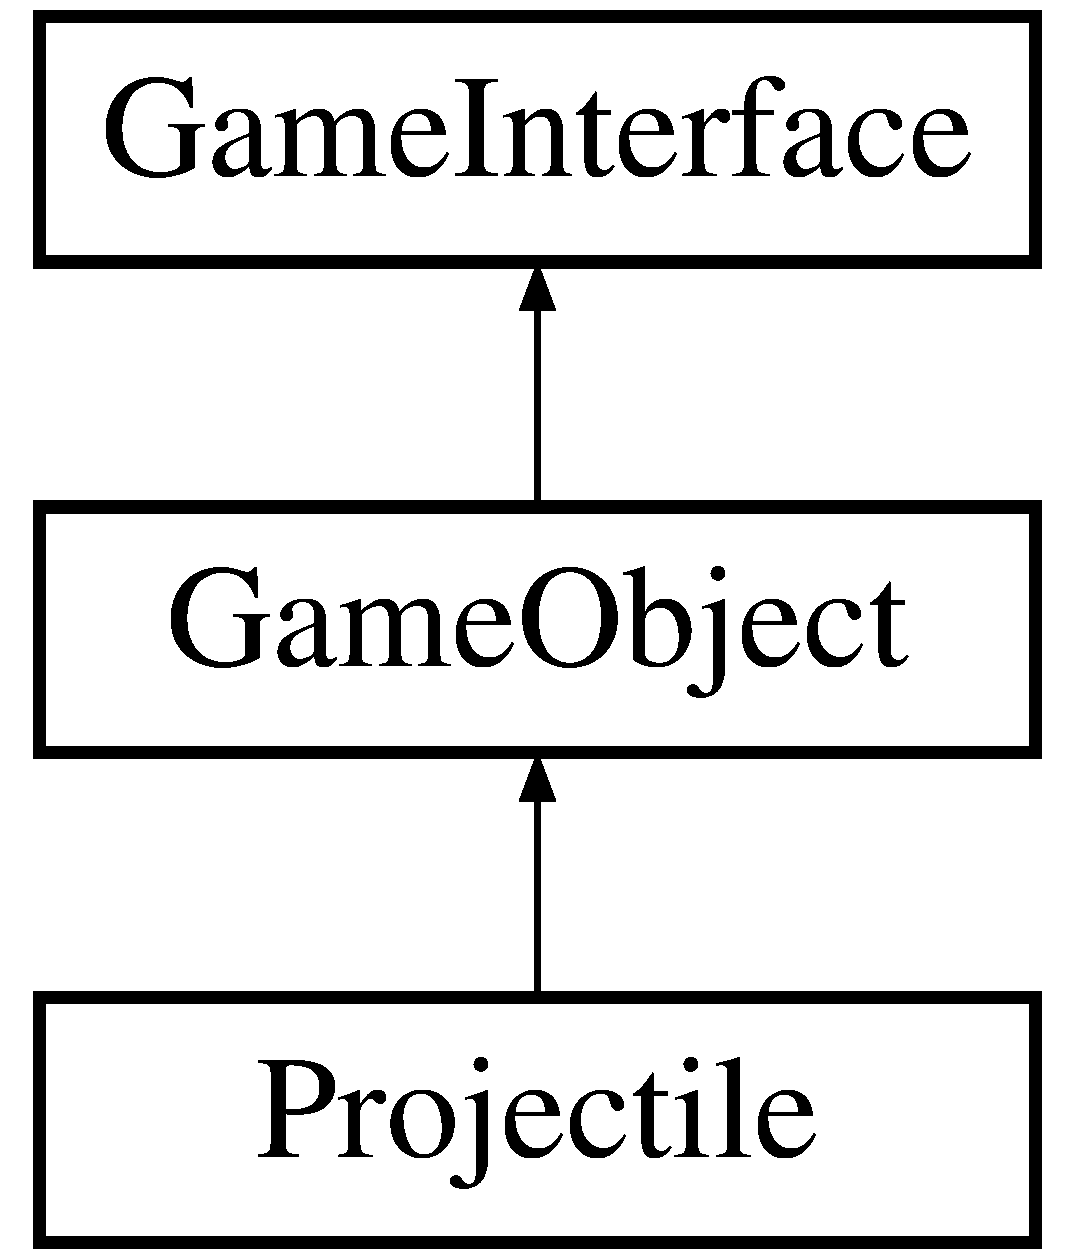
\includegraphics[height=3.000000cm]{class_projectile}
\end{center}
\end{figure}
\subsection*{Public Member Functions}
\begin{DoxyCompactItemize}
\item 
void \hyperlink{class_projectile_afb8f0b1e6777785b613472d28b1967f6}{move\-Random\-Direction} () override
\item 
void \hyperlink{class_projectile_acd6a2cea6b495db189ccc8a05d189ef9}{default\-Behaviors} () override
\end{DoxyCompactItemize}
\subsection*{Additional Inherited Members}


\subsection{Detailed Description}


Definition at line 16 of file Weapon.\-h.



\subsection{Member Function Documentation}
\hypertarget{class_projectile_acd6a2cea6b495db189ccc8a05d189ef9}{\index{Projectile@{Projectile}!default\-Behaviors@{default\-Behaviors}}
\index{default\-Behaviors@{default\-Behaviors}!Projectile@{Projectile}}
\subsubsection[{default\-Behaviors}]{\setlength{\rightskip}{0pt plus 5cm}void Projectile\-::default\-Behaviors (
\begin{DoxyParamCaption}
{}
\end{DoxyParamCaption}
)\hspace{0.3cm}{\ttfamily [inline]}, {\ttfamily [override]}, {\ttfamily [virtual]}}}\label{class_projectile_acd6a2cea6b495db189ccc8a05d189ef9}
Overidden to ensure this has no functionality 

Reimplemented from \hyperlink{class_game_object_a565a3950ea0af84bf7515bdb77abf51a}{Game\-Object}.



Definition at line 37 of file Weapon.\-h.

\hypertarget{class_projectile_afb8f0b1e6777785b613472d28b1967f6}{\index{Projectile@{Projectile}!move\-Random\-Direction@{move\-Random\-Direction}}
\index{move\-Random\-Direction@{move\-Random\-Direction}!Projectile@{Projectile}}
\subsubsection[{move\-Random\-Direction}]{\setlength{\rightskip}{0pt plus 5cm}void Projectile\-::move\-Random\-Direction (
\begin{DoxyParamCaption}
{}
\end{DoxyParamCaption}
)\hspace{0.3cm}{\ttfamily [inline]}, {\ttfamily [override]}, {\ttfamily [virtual]}}}\label{class_projectile_afb8f0b1e6777785b613472d28b1967f6}
Overidden to ensure this has no functionality 

Reimplemented from \hyperlink{class_game_object_ac279191d7c42ca8ad3e1dd2baf5a9519}{Game\-Object}.



Definition at line 30 of file Weapon.\-h.



The documentation for this class was generated from the following file\-:\begin{DoxyCompactItemize}
\item 
/\-Volumes/\-O\-S X H\-D\-D/\-Users/\-Adam/\-Developer/\-Sprite\-Fight/\-World/\hyperlink{_weapon_8h}{Weapon.\-h}\end{DoxyCompactItemize}

\hypertarget{struct_resolution}{\section{Resolution$<$ N $>$ Struct Template Reference}
\label{struct_resolution}\index{Resolution$<$ N $>$@{Resolution$<$ N $>$}}
}


{\ttfamily \#include $<$Default\-Config.\-h$>$}

Inheritance diagram for Resolution$<$ N $>$\-:\begin{figure}[H]
\begin{center}
\leavevmode
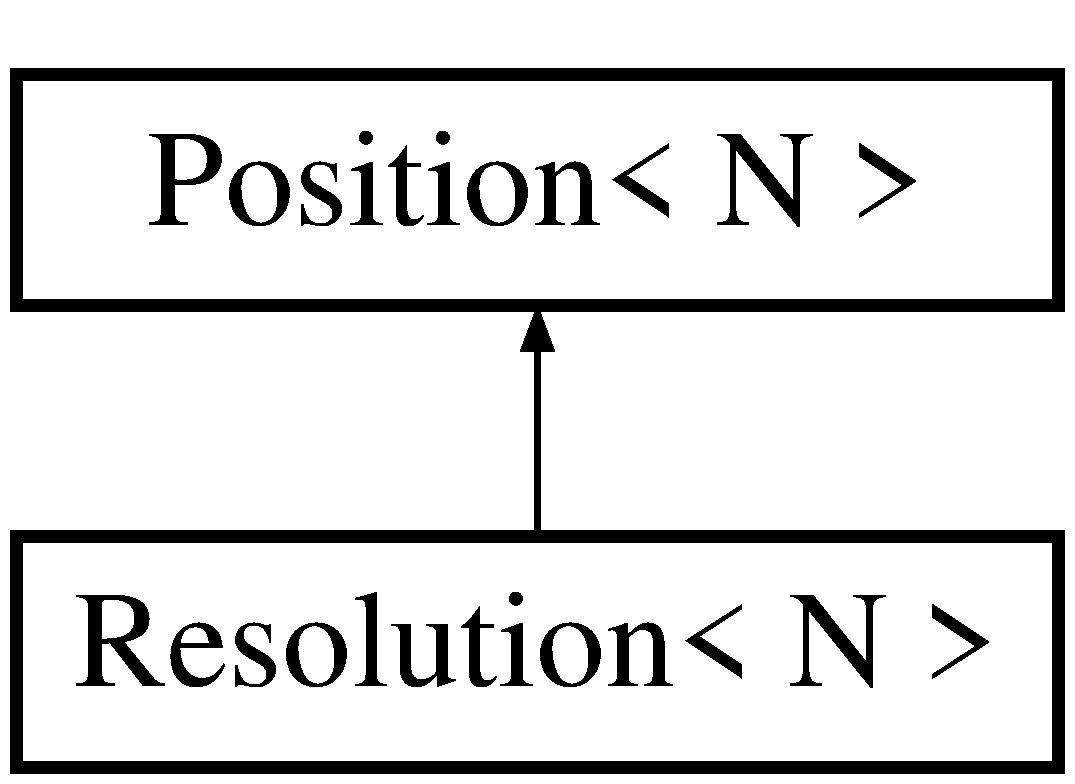
\includegraphics[height=2.000000cm]{struct_resolution}
\end{center}
\end{figure}
\subsection*{Public Member Functions}
\begin{DoxyCompactItemize}
\item 
\hyperlink{struct_resolution_ac30561f6544f2fc3bf481c6e0b14b461}{Resolution} ()
\item 
\hyperlink{struct_resolution_a9bb8d85e9faff270276a2e8323118fc8}{Resolution} (N \hyperlink{struct_position_af908be922fc88d89d81be7d08d06f761}{x}, N \hyperlink{struct_position_af434f54a0aad8bbfc3806ebdd197aa3b}{y})
\item 
\hyperlink{struct_resolution_a2aa8fc1f683337902dc151bada7288dd}{Resolution} (const \hyperlink{struct_resolution}{Resolution} \&other)
\item 
\hyperlink{struct_resolution_ac4d06880fbc7211f869e39cf38b0ed19}{Resolution} (\hyperlink{struct_resolution}{Resolution} \&\&other)
\item 
\hyperlink{struct_resolution}{Resolution} \& \hyperlink{struct_resolution_a717cb848dd45e1ee2454dca048b31e4f}{operator=} (const \hyperlink{struct_resolution}{Resolution} \&rhs)
\item 
\hyperlink{struct_resolution_a6cb2b5a6a911ad7cf5ecf77707c653d0}{$\sim$\-Resolution} ()
\item 
\hyperlink{struct_resolution}{Resolution} \& \hyperlink{struct_resolution_a23374340976ac8ce3fee681ea3e81c60}{operator=} (\hyperlink{struct_resolution}{Resolution} \&\&rhs)
\item 
\hyperlink{struct_resolution}{Resolution} \hyperlink{struct_resolution_ad92daf6afa258c08bfe4d910652f19a9}{operator$\ast$} (const N n) const 
\item 
double \hyperlink{struct_resolution_aa129e2a84f2bb2ff1e72845c94d95ff4}{operator/} (const \hyperlink{struct_resolution}{Resolution} \&rhs) const 
\end{DoxyCompactItemize}
\subsection*{Friends}
\begin{DoxyCompactItemize}
\item 
ostream \& \hyperlink{struct_resolution_a9a1a88fb46fb0e0778bedc8a83353379}{operator$<$$<$} (std\-::ostream \&os, const \hyperlink{struct_resolution}{Resolution}$<$ N $>$ $\ast$pos)
\item 
ostream \& \hyperlink{struct_resolution_afd33ccf011112b1d008268776db1b3c2}{operator$<$$<$} (std\-::ostream \&os, const \hyperlink{struct_resolution}{Resolution}$<$ N $>$ \&pos)
\end{DoxyCompactItemize}
\subsection*{Additional Inherited Members}


\subsection{Detailed Description}
\subsubsection*{template$<$typename N$>$struct Resolution$<$ N $>$}



Definition at line 27 of file Default\-Config.\-h.



\subsection{Constructor \& Destructor Documentation}
\hypertarget{struct_resolution_ac30561f6544f2fc3bf481c6e0b14b461}{\index{Resolution@{Resolution}!Resolution@{Resolution}}
\index{Resolution@{Resolution}!Resolution@{Resolution}}
\subsubsection[{Resolution}]{\setlength{\rightskip}{0pt plus 5cm}template$<$typename N $>$ {\bf Resolution}$<$ N $>$\-::{\bf Resolution} (
\begin{DoxyParamCaption}
{}
\end{DoxyParamCaption}
)\hspace{0.3cm}{\ttfamily [inline]}}}\label{struct_resolution_ac30561f6544f2fc3bf481c6e0b14b461}


Definition at line 1466 of file Position.\-hpp.

\hypertarget{struct_resolution_a9bb8d85e9faff270276a2e8323118fc8}{\index{Resolution@{Resolution}!Resolution@{Resolution}}
\index{Resolution@{Resolution}!Resolution@{Resolution}}
\subsubsection[{Resolution}]{\setlength{\rightskip}{0pt plus 5cm}template$<$typename N $>$ {\bf Resolution}$<$ N $>$\-::{\bf Resolution} (
\begin{DoxyParamCaption}
\item[{N}]{x, }
\item[{N}]{y}
\end{DoxyParamCaption}
)\hspace{0.3cm}{\ttfamily [inline]}}}\label{struct_resolution_a9bb8d85e9faff270276a2e8323118fc8}


Definition at line 1469 of file Position.\-hpp.

\hypertarget{struct_resolution_a2aa8fc1f683337902dc151bada7288dd}{\index{Resolution@{Resolution}!Resolution@{Resolution}}
\index{Resolution@{Resolution}!Resolution@{Resolution}}
\subsubsection[{Resolution}]{\setlength{\rightskip}{0pt plus 5cm}template$<$typename N $>$ {\bf Resolution}$<$ N $>$\-::{\bf Resolution} (
\begin{DoxyParamCaption}
\item[{const {\bf Resolution}$<$ N $>$ \&}]{other}
\end{DoxyParamCaption}
)\hspace{0.3cm}{\ttfamily [inline]}}}\label{struct_resolution_a2aa8fc1f683337902dc151bada7288dd}


Definition at line 1472 of file Position.\-hpp.

\hypertarget{struct_resolution_ac4d06880fbc7211f869e39cf38b0ed19}{\index{Resolution@{Resolution}!Resolution@{Resolution}}
\index{Resolution@{Resolution}!Resolution@{Resolution}}
\subsubsection[{Resolution}]{\setlength{\rightskip}{0pt plus 5cm}template$<$typename N $>$ {\bf Resolution}$<$ N $>$\-::{\bf Resolution} (
\begin{DoxyParamCaption}
\item[{{\bf Resolution}$<$ N $>$ \&\&}]{other}
\end{DoxyParamCaption}
)\hspace{0.3cm}{\ttfamily [inline]}}}\label{struct_resolution_ac4d06880fbc7211f869e39cf38b0ed19}


Definition at line 1475 of file Position.\-hpp.

\hypertarget{struct_resolution_a6cb2b5a6a911ad7cf5ecf77707c653d0}{\index{Resolution@{Resolution}!$\sim$\-Resolution@{$\sim$\-Resolution}}
\index{$\sim$\-Resolution@{$\sim$\-Resolution}!Resolution@{Resolution}}
\subsubsection[{$\sim$\-Resolution}]{\setlength{\rightskip}{0pt plus 5cm}template$<$typename N $>$ {\bf Resolution}$<$ N $>$\-::$\sim${\bf Resolution} (
\begin{DoxyParamCaption}
{}
\end{DoxyParamCaption}
)\hspace{0.3cm}{\ttfamily [inline]}}}\label{struct_resolution_a6cb2b5a6a911ad7cf5ecf77707c653d0}


Definition at line 1485 of file Position.\-hpp.



\subsection{Member Function Documentation}
\hypertarget{struct_resolution_ad92daf6afa258c08bfe4d910652f19a9}{\index{Resolution@{Resolution}!operator$\ast$@{operator$\ast$}}
\index{operator$\ast$@{operator$\ast$}!Resolution@{Resolution}}
\subsubsection[{operator$\ast$}]{\setlength{\rightskip}{0pt plus 5cm}template$<$typename N $>$ {\bf Resolution} {\bf Resolution}$<$ N $>$\-::operator$\ast$ (
\begin{DoxyParamCaption}
\item[{const N}]{n}
\end{DoxyParamCaption}
) const\hspace{0.3cm}{\ttfamily [inline]}}}\label{struct_resolution_ad92daf6afa258c08bfe4d910652f19a9}


Definition at line 1494 of file Position.\-hpp.

\hypertarget{struct_resolution_aa129e2a84f2bb2ff1e72845c94d95ff4}{\index{Resolution@{Resolution}!operator/@{operator/}}
\index{operator/@{operator/}!Resolution@{Resolution}}
\subsubsection[{operator/}]{\setlength{\rightskip}{0pt plus 5cm}template$<$typename N $>$ double {\bf Resolution}$<$ N $>$\-::operator/ (
\begin{DoxyParamCaption}
\item[{const {\bf Resolution}$<$ N $>$ \&}]{rhs}
\end{DoxyParamCaption}
) const\hspace{0.3cm}{\ttfamily [inline]}}}\label{struct_resolution_aa129e2a84f2bb2ff1e72845c94d95ff4}


Definition at line 1502 of file Position.\-hpp.

\hypertarget{struct_resolution_a717cb848dd45e1ee2454dca048b31e4f}{\index{Resolution@{Resolution}!operator=@{operator=}}
\index{operator=@{operator=}!Resolution@{Resolution}}
\subsubsection[{operator=}]{\setlength{\rightskip}{0pt plus 5cm}template$<$typename N $>$ {\bf Resolution}\& {\bf Resolution}$<$ N $>$\-::operator= (
\begin{DoxyParamCaption}
\item[{const {\bf Resolution}$<$ N $>$ \&}]{rhs}
\end{DoxyParamCaption}
)\hspace{0.3cm}{\ttfamily [inline]}}}\label{struct_resolution_a717cb848dd45e1ee2454dca048b31e4f}


Definition at line 1478 of file Position.\-hpp.

\hypertarget{struct_resolution_a23374340976ac8ce3fee681ea3e81c60}{\index{Resolution@{Resolution}!operator=@{operator=}}
\index{operator=@{operator=}!Resolution@{Resolution}}
\subsubsection[{operator=}]{\setlength{\rightskip}{0pt plus 5cm}template$<$typename N $>$ {\bf Resolution}\& {\bf Resolution}$<$ N $>$\-::operator= (
\begin{DoxyParamCaption}
\item[{{\bf Resolution}$<$ N $>$ \&\&}]{rhs}
\end{DoxyParamCaption}
)\hspace{0.3cm}{\ttfamily [inline]}}}\label{struct_resolution_a23374340976ac8ce3fee681ea3e81c60}


Definition at line 1487 of file Position.\-hpp.



\subsection{Friends And Related Function Documentation}
\hypertarget{struct_resolution_a9a1a88fb46fb0e0778bedc8a83353379}{\index{Resolution@{Resolution}!operator$<$$<$@{operator$<$$<$}}
\index{operator$<$$<$@{operator$<$$<$}!Resolution@{Resolution}}
\subsubsection[{operator$<$$<$}]{\setlength{\rightskip}{0pt plus 5cm}template$<$typename N $>$ ostream\& operator$<$$<$ (
\begin{DoxyParamCaption}
\item[{std\-::ostream \&}]{os, }
\item[{const {\bf Resolution}$<$ N $>$ $\ast$}]{pos}
\end{DoxyParamCaption}
)\hspace{0.3cm}{\ttfamily [friend]}}}\label{struct_resolution_a9a1a88fb46fb0e0778bedc8a83353379}


Definition at line 1512 of file Position.\-hpp.

\hypertarget{struct_resolution_afd33ccf011112b1d008268776db1b3c2}{\index{Resolution@{Resolution}!operator$<$$<$@{operator$<$$<$}}
\index{operator$<$$<$@{operator$<$$<$}!Resolution@{Resolution}}
\subsubsection[{operator$<$$<$}]{\setlength{\rightskip}{0pt plus 5cm}template$<$typename N $>$ ostream\& operator$<$$<$ (
\begin{DoxyParamCaption}
\item[{std\-::ostream \&}]{os, }
\item[{const {\bf Resolution}$<$ N $>$ \&}]{pos}
\end{DoxyParamCaption}
)\hspace{0.3cm}{\ttfamily [friend]}}}\label{struct_resolution_afd33ccf011112b1d008268776db1b3c2}


Definition at line 1517 of file Position.\-hpp.



The documentation for this struct was generated from the following files\-:\begin{DoxyCompactItemize}
\item 
/\-Volumes/\-O\-S X H\-D\-D/\-Users/\-Adam/\-Developer/\-Sprite\-Fight/\-Control/\hyperlink{_default_config_8h}{Default\-Config.\-h}\item 
/\-Volumes/\-O\-S X H\-D\-D/\-Users/\-Adam/\-Developer/\-Sprite\-Fight/\-Util/\hyperlink{_position_8hpp}{Position.\-hpp}\end{DoxyCompactItemize}

\hypertarget{struct_size}{\section{Size$<$ N $>$ Struct Template Reference}
\label{struct_size}\index{Size$<$ N $>$@{Size$<$ N $>$}}
}


{\ttfamily \#include $<$Size.\-hpp$>$}

Inheritance diagram for Size$<$ N $>$\-:\begin{figure}[H]
\begin{center}
\leavevmode
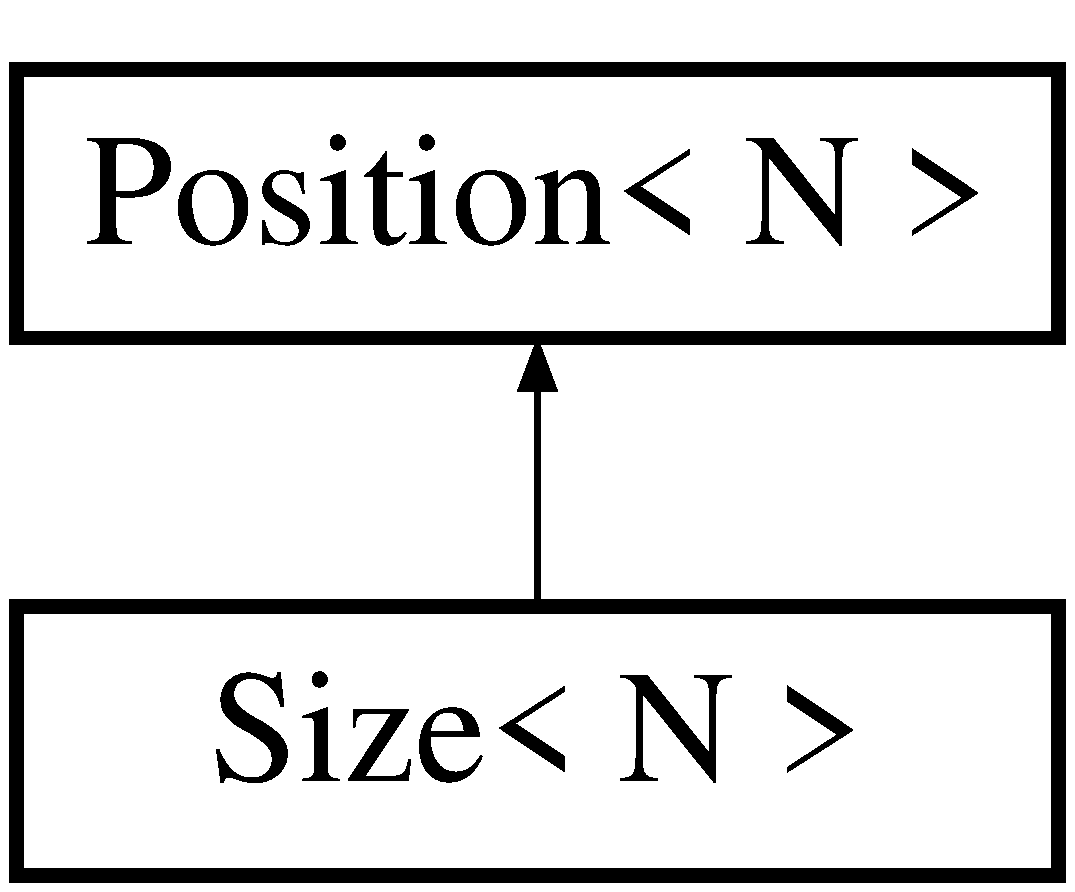
\includegraphics[height=2.000000cm]{struct_size}
\end{center}
\end{figure}
\subsection*{Public Member Functions}
\begin{DoxyCompactItemize}
\item 
\hyperlink{struct_size_af17421be7acae6d13fc4670f04854de6}{Size} ()
\item 
\hyperlink{struct_size_abf87d26cd771b7fa7b7e3f37acd3e076}{Size} (N w\-\_\-, N h\-\_\-, float modifier)
\item 
\hyperlink{struct_size_aebc8ee17587db4f84c8d9085f27a761d}{Size} (N w\-\_\-, N h\-\_\-)
\item 
\hyperlink{struct_size_ae90aed86840a6650d6ee3d5897afe148}{Size} (const \hyperlink{struct_size}{Size}$<$ N $>$ \&other)
\item 
\hyperlink{struct_size_a31ee38aed5f689000e9fb7415b2f60ce}{Size} (\hyperlink{struct_size}{Size}$<$ N $>$ \&\&other)
\item 
\hyperlink{struct_size_a5a4e62203d653f23e3d88e966b86e3a5}{$\sim$\-Size} ()
\item 
\hyperlink{struct_size}{Size} \& \hyperlink{struct_size_aa0067a04662b093f532b9ebec3175f66}{operator=} (const \hyperlink{struct_size}{Size}$<$ N $>$ \&rhs)
\item 
\hyperlink{struct_size}{Size} \& \hyperlink{struct_size_a7837d5a7b300e0e0052d21e8638361b1}{operator=} (\hyperlink{struct_size}{Size}$<$ N $>$ \&\&rhs)
\item 
void \hyperlink{struct_size_a923481b9729ecc21e249f957049f5d75}{set\-Modifier} (const float modifier)
\item 
void \hyperlink{struct_size_a0893fda3a27cd8bb3e232aa075bfb3cb}{set\-Size} (N w, N h)
\item 
void \hyperlink{struct_size_a402405c7c280000893b3afb4a6bfcce8}{set\-Size} (N w, N h, float modifier)
\item 
float \hyperlink{struct_size_a350abccbfe5b544af3fd6f9c2f50efdb}{get\-Modifier} () const 
\item 
N \hyperlink{struct_size_a80f33b91ecc82d4cf95bc00b1a9406f0}{get\-Width} () const 
\item 
N \hyperlink{struct_size_a403711af30722f363b175bc83dcbcc44}{get\-Height} () const 
\end{DoxyCompactItemize}
\subsection*{Additional Inherited Members}


\subsection{Detailed Description}
\subsubsection*{template$<$typename N$>$struct Size$<$ N $>$}



Definition at line 19 of file Size.\-hpp.



\subsection{Constructor \& Destructor Documentation}
\hypertarget{struct_size_af17421be7acae6d13fc4670f04854de6}{\index{Size@{Size}!Size@{Size}}
\index{Size@{Size}!Size@{Size}}
\subsubsection[{Size}]{\setlength{\rightskip}{0pt plus 5cm}template$<$typename N$>$ {\bf Size}$<$ N $>$\-::{\bf Size} (
\begin{DoxyParamCaption}
{}
\end{DoxyParamCaption}
)\hspace{0.3cm}{\ttfamily [inline]}}}\label{struct_size_af17421be7acae6d13fc4670f04854de6}


Definition at line 40 of file Size.\-hpp.

\hypertarget{struct_size_abf87d26cd771b7fa7b7e3f37acd3e076}{\index{Size@{Size}!Size@{Size}}
\index{Size@{Size}!Size@{Size}}
\subsubsection[{Size}]{\setlength{\rightskip}{0pt plus 5cm}template$<$typename N$>$ {\bf Size}$<$ N $>$\-::{\bf Size} (
\begin{DoxyParamCaption}
\item[{N}]{w\-\_\-, }
\item[{N}]{h\-\_\-, }
\item[{float}]{modifier}
\end{DoxyParamCaption}
)\hspace{0.3cm}{\ttfamily [inline]}}}\label{struct_size_abf87d26cd771b7fa7b7e3f37acd3e076}


Definition at line 44 of file Size.\-hpp.

\hypertarget{struct_size_aebc8ee17587db4f84c8d9085f27a761d}{\index{Size@{Size}!Size@{Size}}
\index{Size@{Size}!Size@{Size}}
\subsubsection[{Size}]{\setlength{\rightskip}{0pt plus 5cm}template$<$typename N$>$ {\bf Size}$<$ N $>$\-::{\bf Size} (
\begin{DoxyParamCaption}
\item[{N}]{w\-\_\-, }
\item[{N}]{h\-\_\-}
\end{DoxyParamCaption}
)\hspace{0.3cm}{\ttfamily [inline]}}}\label{struct_size_aebc8ee17587db4f84c8d9085f27a761d}


Definition at line 48 of file Size.\-hpp.

\hypertarget{struct_size_ae90aed86840a6650d6ee3d5897afe148}{\index{Size@{Size}!Size@{Size}}
\index{Size@{Size}!Size@{Size}}
\subsubsection[{Size}]{\setlength{\rightskip}{0pt plus 5cm}template$<$typename N$>$ {\bf Size}$<$ N $>$\-::{\bf Size} (
\begin{DoxyParamCaption}
\item[{const {\bf Size}$<$ N $>$ \&}]{other}
\end{DoxyParamCaption}
)\hspace{0.3cm}{\ttfamily [inline]}}}\label{struct_size_ae90aed86840a6650d6ee3d5897afe148}


Definition at line 52 of file Size.\-hpp.

\hypertarget{struct_size_a31ee38aed5f689000e9fb7415b2f60ce}{\index{Size@{Size}!Size@{Size}}
\index{Size@{Size}!Size@{Size}}
\subsubsection[{Size}]{\setlength{\rightskip}{0pt plus 5cm}template$<$typename N$>$ {\bf Size}$<$ N $>$\-::{\bf Size} (
\begin{DoxyParamCaption}
\item[{{\bf Size}$<$ N $>$ \&\&}]{other}
\end{DoxyParamCaption}
)\hspace{0.3cm}{\ttfamily [inline]}}}\label{struct_size_a31ee38aed5f689000e9fb7415b2f60ce}


Definition at line 56 of file Size.\-hpp.

\hypertarget{struct_size_a5a4e62203d653f23e3d88e966b86e3a5}{\index{Size@{Size}!$\sim$\-Size@{$\sim$\-Size}}
\index{$\sim$\-Size@{$\sim$\-Size}!Size@{Size}}
\subsubsection[{$\sim$\-Size}]{\setlength{\rightskip}{0pt plus 5cm}template$<$typename N$>$ {\bf Size}$<$ N $>$\-::$\sim${\bf Size} (
\begin{DoxyParamCaption}
{}
\end{DoxyParamCaption}
)\hspace{0.3cm}{\ttfamily [inline]}}}\label{struct_size_a5a4e62203d653f23e3d88e966b86e3a5}


Definition at line 60 of file Size.\-hpp.



\subsection{Member Function Documentation}
\hypertarget{struct_size_a403711af30722f363b175bc83dcbcc44}{\index{Size@{Size}!get\-Height@{get\-Height}}
\index{get\-Height@{get\-Height}!Size@{Size}}
\subsubsection[{get\-Height}]{\setlength{\rightskip}{0pt plus 5cm}template$<$typename N$>$ N {\bf Size}$<$ N $>$\-::get\-Height (
\begin{DoxyParamCaption}
{}
\end{DoxyParamCaption}
) const\hspace{0.3cm}{\ttfamily [inline]}}}\label{struct_size_a403711af30722f363b175bc83dcbcc44}


Definition at line 89 of file Size.\-hpp.

\hypertarget{struct_size_a350abccbfe5b544af3fd6f9c2f50efdb}{\index{Size@{Size}!get\-Modifier@{get\-Modifier}}
\index{get\-Modifier@{get\-Modifier}!Size@{Size}}
\subsubsection[{get\-Modifier}]{\setlength{\rightskip}{0pt plus 5cm}template$<$typename N$>$ float {\bf Size}$<$ N $>$\-::get\-Modifier (
\begin{DoxyParamCaption}
{}
\end{DoxyParamCaption}
) const\hspace{0.3cm}{\ttfamily [inline]}}}\label{struct_size_a350abccbfe5b544af3fd6f9c2f50efdb}


Definition at line 87 of file Size.\-hpp.

\hypertarget{struct_size_a80f33b91ecc82d4cf95bc00b1a9406f0}{\index{Size@{Size}!get\-Width@{get\-Width}}
\index{get\-Width@{get\-Width}!Size@{Size}}
\subsubsection[{get\-Width}]{\setlength{\rightskip}{0pt plus 5cm}template$<$typename N$>$ N {\bf Size}$<$ N $>$\-::get\-Width (
\begin{DoxyParamCaption}
{}
\end{DoxyParamCaption}
) const\hspace{0.3cm}{\ttfamily [inline]}}}\label{struct_size_a80f33b91ecc82d4cf95bc00b1a9406f0}


Definition at line 88 of file Size.\-hpp.

\hypertarget{struct_size_aa0067a04662b093f532b9ebec3175f66}{\index{Size@{Size}!operator=@{operator=}}
\index{operator=@{operator=}!Size@{Size}}
\subsubsection[{operator=}]{\setlength{\rightskip}{0pt plus 5cm}template$<$typename N$>$ {\bf Size}\& {\bf Size}$<$ N $>$\-::operator= (
\begin{DoxyParamCaption}
\item[{const {\bf Size}$<$ N $>$ \&}]{rhs}
\end{DoxyParamCaption}
)\hspace{0.3cm}{\ttfamily [inline]}}}\label{struct_size_aa0067a04662b093f532b9ebec3175f66}


Definition at line 62 of file Size.\-hpp.

\hypertarget{struct_size_a7837d5a7b300e0e0052d21e8638361b1}{\index{Size@{Size}!operator=@{operator=}}
\index{operator=@{operator=}!Size@{Size}}
\subsubsection[{operator=}]{\setlength{\rightskip}{0pt plus 5cm}template$<$typename N$>$ {\bf Size}\& {\bf Size}$<$ N $>$\-::operator= (
\begin{DoxyParamCaption}
\item[{{\bf Size}$<$ N $>$ \&\&}]{rhs}
\end{DoxyParamCaption}
)\hspace{0.3cm}{\ttfamily [inline]}}}\label{struct_size_a7837d5a7b300e0e0052d21e8638361b1}


Definition at line 68 of file Size.\-hpp.

\hypertarget{struct_size_a923481b9729ecc21e249f957049f5d75}{\index{Size@{Size}!set\-Modifier@{set\-Modifier}}
\index{set\-Modifier@{set\-Modifier}!Size@{Size}}
\subsubsection[{set\-Modifier}]{\setlength{\rightskip}{0pt plus 5cm}template$<$typename N$>$ void {\bf Size}$<$ N $>$\-::set\-Modifier (
\begin{DoxyParamCaption}
\item[{const float}]{modifier}
\end{DoxyParamCaption}
)\hspace{0.3cm}{\ttfamily [inline]}}}\label{struct_size_a923481b9729ecc21e249f957049f5d75}


Definition at line 74 of file Size.\-hpp.

\hypertarget{struct_size_a0893fda3a27cd8bb3e232aa075bfb3cb}{\index{Size@{Size}!set\-Size@{set\-Size}}
\index{set\-Size@{set\-Size}!Size@{Size}}
\subsubsection[{set\-Size}]{\setlength{\rightskip}{0pt plus 5cm}template$<$typename N$>$ void {\bf Size}$<$ N $>$\-::set\-Size (
\begin{DoxyParamCaption}
\item[{N}]{w, }
\item[{N}]{h}
\end{DoxyParamCaption}
)\hspace{0.3cm}{\ttfamily [inline]}}}\label{struct_size_a0893fda3a27cd8bb3e232aa075bfb3cb}


Definition at line 76 of file Size.\-hpp.

\hypertarget{struct_size_a402405c7c280000893b3afb4a6bfcce8}{\index{Size@{Size}!set\-Size@{set\-Size}}
\index{set\-Size@{set\-Size}!Size@{Size}}
\subsubsection[{set\-Size}]{\setlength{\rightskip}{0pt plus 5cm}template$<$typename N$>$ void {\bf Size}$<$ N $>$\-::set\-Size (
\begin{DoxyParamCaption}
\item[{N}]{w, }
\item[{N}]{h, }
\item[{float}]{modifier}
\end{DoxyParamCaption}
)\hspace{0.3cm}{\ttfamily [inline]}}}\label{struct_size_a402405c7c280000893b3afb4a6bfcce8}


Definition at line 81 of file Size.\-hpp.



The documentation for this struct was generated from the following file\-:\begin{DoxyCompactItemize}
\item 
/\-Volumes/\-O\-S X H\-D\-D/\-Users/\-Adam/\-Developer/\-Sprite\-Fight/\-Util/\hyperlink{_size_8hpp}{Size.\-hpp}\end{DoxyCompactItemize}

\hypertarget{class_switchable_key_input_register}{\section{Switchable\-Key\-Input\-Register Class Reference}
\label{class_switchable_key_input_register}\index{Switchable\-Key\-Input\-Register@{Switchable\-Key\-Input\-Register}}
}


{\ttfamily \#include $<$Input.\-hpp$>$}

Inheritance diagram for Switchable\-Key\-Input\-Register\-:\begin{figure}[H]
\begin{center}
\leavevmode
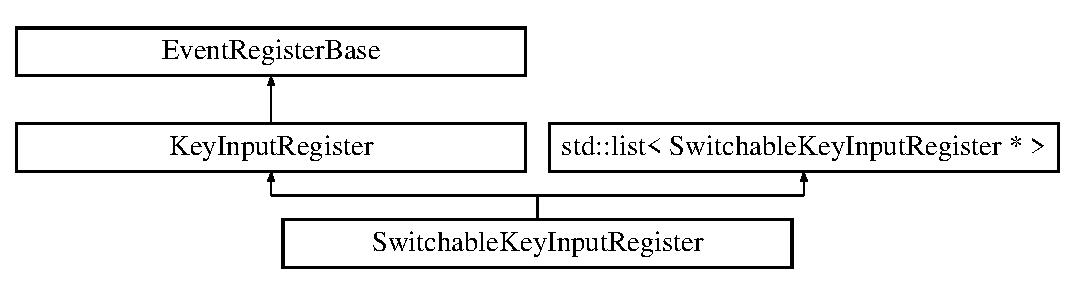
\includegraphics[height=3.000000cm]{class_switchable_key_input_register}
\end{center}
\end{figure}
\subsection*{Additional Inherited Members}


\subsection{Detailed Description}
\hyperlink{class_switchable_key_input_register}{Switchable\-Key\-Input\-Register} is a variant of \hyperlink{class_key_input_register}{Key\-Input\-Register} that can hold multiple callback functions (and members to call those functions on), as well as several different keyboard keys at the same time. This is in contrast to the single function pointer held in any \hyperlink{class_key_input_register}{Key\-Input\-Register}. The real advantage of \hyperlink{class_switchable_key_input_register}{Switchable\-Key\-Input\-Register} is its ability to choose different callbacks based on a descending order of priority that is set when the \hyperlink{class_switchable_key_input_register}{Switchable\-Key\-Input\-Register} is created. A \hyperlink{class_switchable_key_input_register}{Switchable\-Key\-Input\-Register} is part of a linked-\/list of pointers to Key\-Input\-Registers or other Switchable\-Key\-Input\-Registers, and each one is able to \char`\"{}shut off\char`\"{} subsequent members in its list from providing their callback functions. The list should be initialized with the highest priority Key\-Input\-Registers at the front, with the fallback, lower priority ones following. Any \hyperlink{class_key_input_register}{Key\-Input\-Register} or \hyperlink{class_switchable_key_input_register}{Switchable\-Key\-Input\-Register}'s callback function will only be called if callback function belonging to the \hyperlink{class_key_input_register}{Key\-Input\-Register} prior to it in the list was not. 

Definition at line 368 of file Input.\-hpp.



The documentation for this class was generated from the following file\-:\begin{DoxyCompactItemize}
\item 
/\-Volumes/\-O\-S X H\-D\-D/\-Users/\-Adam/\-Developer/\-Sprite\-Fight/\-Control/\hyperlink{_input_8hpp}{Input.\-hpp}\end{DoxyCompactItemize}

\hypertarget{class_text_output}{\section{Text\-Output$<$ P\-O\-S\-U\-T\-Y\-P\-E, S\-I\-Z\-E\-U\-T\-Y\-P\-E $>$ Class Template Reference}
\label{class_text_output}\index{Text\-Output$<$ P\-O\-S\-U\-T\-Y\-P\-E, S\-I\-Z\-E\-U\-T\-Y\-P\-E $>$@{Text\-Output$<$ P\-O\-S\-U\-T\-Y\-P\-E, S\-I\-Z\-E\-U\-T\-Y\-P\-E $>$}}
}


{\ttfamily \#include $<$Text\-Output.\-hpp$>$}

Inheritance diagram for Text\-Output$<$ P\-O\-S\-U\-T\-Y\-P\-E, S\-I\-Z\-E\-U\-T\-Y\-P\-E $>$\-:\begin{figure}[H]
\begin{center}
\leavevmode
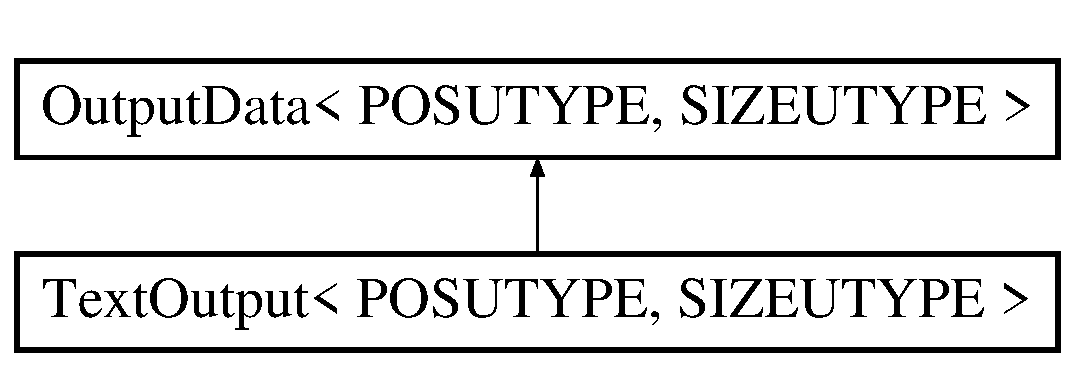
\includegraphics[height=2.000000cm]{class_text_output}
\end{center}
\end{figure}
\subsection*{Public Member Functions}
\begin{DoxyCompactItemize}
\item 
\hyperlink{class_text_output_abac1dd11f3ca8dc1ed87f07c17000924}{Text\-Output} (const string \&\hyperlink{class_text_output_aa63e4c0936ed44ad8658f9567acd437b}{text}, const \hyperlink{struct_position}{Position}$<$ P\-O\-S\-U\-T\-Y\-P\-E $>$ \&pos, \hyperlink{struct_game_color}{Game\-Color} \hyperlink{class_text_output_a969669fc87e0828685b6b20c4bb79616}{foreground}, \hyperlink{struct_game_color}{Game\-Color} \hyperlink{class_text_output_a1d58e4651de9d729bdc19f143b2bb042}{background})
\item 
\hyperlink{class_text_output_a8fffd270710bf5d13430696091491064}{$\sim$\-Text\-Output} ()
\begin{DoxyCompactList}\small\item\em Destructor for \hyperlink{class_text_output}{Text\-Output}. \end{DoxyCompactList}\item 
void \hyperlink{class_text_output_a9981707e972ac76a7bb7adb65201a84a}{update\-Text} (const string \&new\-Text)
\item 
void \hyperlink{class_text_output_ae028755399b3afc882a98da908759d0f}{update\-Position} (const \hyperlink{struct_position}{Position}$<$ P\-O\-S\-U\-T\-Y\-P\-E $>$ \&pos)
\item 
void \hyperlink{class_text_output_a6477f07208204b1c058ba6fa6b0e5cc6}{update\-Foreground\-Color} (\hyperlink{struct_game_color}{Game\-Color} color)
\item 
void \hyperlink{class_text_output_a46c108e633d09a102788e600b7a6d370}{update\-Background\-Color} (\hyperlink{struct_game_color}{Game\-Color} color)
\item 
const \hyperlink{struct_output_data}{Output\-Data}$<$ P\-O\-S\-U\-T\-Y\-P\-E, \\*
S\-I\-Z\-E\-U\-T\-Y\-P\-E $>$ $\ast$ \hyperlink{class_text_output_ae0f04c5f70ce6e372f7859daedbf39ee}{get\-Output\-Data} ()
\item 
const string $\ast$ \hyperlink{class_text_output_a811bcb3bc1d278ad3716bf768af2ca9d}{view\-Text} ()
\item 
void \hyperlink{class_text_output_aa7a22a6b6c0a323524ac4c956d54034c}{erase} ()
\end{DoxyCompactItemize}
\subsection*{Static Public Member Functions}
\begin{DoxyCompactItemize}
\item 
static void \hyperlink{class_text_output_ae5f21f4ba09be0b403967268b7ef0ad7}{init} ()
\item 
static \hyperlink{struct_size}{Size}$<$ S\-I\-Z\-E\-U\-T\-Y\-P\-E $>$ \hyperlink{class_text_output_a0ec07dd71eac9a1dd1622e506bd49377}{get\-Size\-Of\-Text} (const string \&str)
\item 
static void \hyperlink{class_text_output_adc94b706e632c9e2b1d62f5756dfbbb5}{exit} ()
\item 
static void \hyperlink{class_text_output_ac1c4bc687c2007648a18d3c76ee828f6}{display\-Continuous\-Text} (const string $\ast$updating\-Text, const \hyperlink{struct_position}{Position}$<$ P\-O\-S\-U\-T\-Y\-P\-E $>$ \&pos, \hyperlink{struct_game_color}{Game\-Color} \hyperlink{class_text_output_a969669fc87e0828685b6b20c4bb79616}{foreground}, \hyperlink{struct_game_color}{Game\-Color} \hyperlink{class_text_output_a1d58e4651de9d729bdc19f143b2bb042}{background})
\begin{DoxyCompactList}\small\item\em Draws a continuously updating text representation of updating\-Text, overriding this-\/$>$text. When using this function there is no need to call \hyperlink{class_text_output_a9981707e972ac76a7bb7adb65201a84a}{update\-Text()}. \end{DoxyCompactList}\item 
static void \hyperlink{class_text_output_a06a756cc49331463a0e4dd8c4bf57e09}{display\-Continuous\-Text} (function$<$ const string(void)$>$ string\-Updating\-Function, const \hyperlink{struct_position}{Position}$<$ P\-O\-S\-U\-T\-Y\-P\-E $>$ \&pos, \hyperlink{struct_game_color}{Game\-Color} \hyperlink{class_text_output_a969669fc87e0828685b6b20c4bb79616}{foreground}, \hyperlink{struct_game_color}{Game\-Color} \hyperlink{class_text_output_a1d58e4651de9d729bdc19f143b2bb042}{background})
\begin{DoxyCompactList}\small\item\em Draws a continuously updating text representation of the string returned by string\-Updating\-Function, overriding this-\/$>$text. When using this function there is no need to call \hyperlink{class_text_output_a9981707e972ac76a7bb7adb65201a84a}{update\-Text()}. \end{DoxyCompactList}\end{DoxyCompactItemize}
\subsection*{Protected Member Functions}
\begin{DoxyCompactItemize}
\item 
void \hyperlink{class_text_output_a2f79d90f6d31ff248fde34f455cf7e16}{add\-Additional\-Update\-Flags} ()
\item 
void \hyperlink{class_text_output_a77b70d1145a189362996cd6b308e7dde}{complete\-Initialization} ()
\begin{DoxyCompactList}\small\item\em Does the remaining initialization that could not be done in the constructor (because it does not know with certainty that it is on the main thread) \end{DoxyCompactList}\item 
virtual void \hyperlink{class_text_output_a0fc3ebc814aa43df128bc6fcc80f5560}{update} ()
\end{DoxyCompactItemize}
\subsection*{Protected Attributes}
\begin{DoxyCompactItemize}
\item 
string \hyperlink{class_text_output_aa63e4c0936ed44ad8658f9567acd437b}{text}
\item 
bool \hyperlink{class_text_output_a01eda9d47821115d2389cc874867f2f5}{text\-\_\-was\-\_\-updated} = false
\item 
\hyperlink{struct_game_color}{Game\-Color} \hyperlink{class_text_output_a969669fc87e0828685b6b20c4bb79616}{foreground}
\item 
\hyperlink{struct_game_color}{Game\-Color} \hyperlink{class_text_output_a1d58e4651de9d729bdc19f143b2bb042}{background}
\item 
bool \hyperlink{class_text_output_abb92f5a8c0c871c8b917f441567d9cae}{color\-\_\-was\-\_\-updated} = false
\item 
bool \hyperlink{class_text_output_a51e0f91233dbf52332b3562ab72aca28}{position\-\_\-was\-\_\-updated}
\end{DoxyCompactItemize}
\subsection*{Static Protected Attributes}
\begin{DoxyCompactItemize}
\item 
static T\-T\-F\-\_\-\-Font $\ast$ \hyperlink{class_text_output_a784e5c34428d43ed01fc5367638df07e}{game\-Font} = nullptr
\item 
static \hyperlink{class_basic_mutex}{Basic\-Mutex} \hyperlink{class_text_output_a64b0160aa7e8ebe7b65744197886662e}{text\-Mutex}
\item 
static const vector\\*
$<$ \hyperlink{struct_output_data}{Output\-Data}$<$ P\-O\-S\-U\-T\-Y\-P\-E, \\*
S\-I\-Z\-E\-U\-T\-Y\-P\-E $>$ $\ast$ $>$ $\ast$ \hyperlink{class_text_output_ae8c77617052494529e2e15a1379c8fa2}{view\-Output\-Data} = \hyperlink{struct_output_data}{Output\-Data}$<$P\-O\-S\-U\-T\-Y\-P\-E, S\-I\-Z\-E\-U\-T\-Y\-P\-E$>$\-::\hyperlink{class_text_output_ae0f04c5f70ce6e372f7859daedbf39ee}{get\-Output\-Data}()
\end{DoxyCompactItemize}
\subsection*{Friends}
\begin{DoxyCompactItemize}
\item 
class \hyperlink{class_text_output_a0969009180cf671defc02a7b2ad9d500}{Graphical\-Output}
\end{DoxyCompactItemize}


\subsection{Detailed Description}
\subsubsection*{template$<$typename P\-O\-S\-U\-T\-Y\-P\-E, typename S\-I\-Z\-E\-U\-T\-Y\-P\-E$>$class Text\-Output$<$ P\-O\-S\-U\-T\-Y\-P\-E, S\-I\-Z\-E\-U\-T\-Y\-P\-E $>$}



Definition at line 38 of file Text\-Output.\-hpp.



\subsection{Constructor \& Destructor Documentation}
\hypertarget{class_text_output_abac1dd11f3ca8dc1ed87f07c17000924}{\index{Text\-Output@{Text\-Output}!Text\-Output@{Text\-Output}}
\index{Text\-Output@{Text\-Output}!TextOutput@{Text\-Output}}
\subsubsection[{Text\-Output}]{\setlength{\rightskip}{0pt plus 5cm}template$<$typename P\-O\-S\-U\-T\-Y\-P\-E , typename S\-I\-Z\-E\-U\-T\-Y\-P\-E $>$ {\bf Text\-Output}$<$ P\-O\-S\-U\-T\-Y\-P\-E, S\-I\-Z\-E\-U\-T\-Y\-P\-E $>$\-::{\bf Text\-Output} (
\begin{DoxyParamCaption}
\item[{const string \&}]{text, }
\item[{const {\bf Position}$<$ P\-O\-S\-U\-T\-Y\-P\-E $>$ \&}]{pos, }
\item[{{\bf Game\-Color}}]{foreground, }
\item[{{\bf Game\-Color}}]{background}
\end{DoxyParamCaption}
)}}\label{class_text_output_abac1dd11f3ca8dc1ed87f07c17000924}
Creates a \hyperlink{class_text_output}{Text\-Output} object which will automatically output the string text to the screen, at the chosen position position, at the next output update. \hyperlink{class_text_output}{Text\-Output} assumes that all pointers given to it remain valid for calling refresh() 

Definition at line 178 of file Text\-Output.\-hpp.

\hypertarget{class_text_output_a8fffd270710bf5d13430696091491064}{\index{Text\-Output@{Text\-Output}!$\sim$\-Text\-Output@{$\sim$\-Text\-Output}}
\index{$\sim$\-Text\-Output@{$\sim$\-Text\-Output}!TextOutput@{Text\-Output}}
\subsubsection[{$\sim$\-Text\-Output}]{\setlength{\rightskip}{0pt plus 5cm}template$<$typename P\-O\-S\-U\-T\-Y\-P\-E , typename S\-I\-Z\-E\-U\-T\-Y\-P\-E $>$ {\bf Text\-Output}$<$ P\-O\-S\-U\-T\-Y\-P\-E, S\-I\-Z\-E\-U\-T\-Y\-P\-E $>$\-::$\sim${\bf Text\-Output} (
\begin{DoxyParamCaption}
{}
\end{DoxyParamCaption}
)\hspace{0.3cm}{\ttfamily [inline]}}}\label{class_text_output_a8fffd270710bf5d13430696091491064}


Destructor for \hyperlink{class_text_output}{Text\-Output}. 



Definition at line 88 of file Text\-Output.\-hpp.



\subsection{Member Function Documentation}
\hypertarget{class_text_output_a2f79d90f6d31ff248fde34f455cf7e16}{\index{Text\-Output@{Text\-Output}!add\-Additional\-Update\-Flags@{add\-Additional\-Update\-Flags}}
\index{add\-Additional\-Update\-Flags@{add\-Additional\-Update\-Flags}!TextOutput@{Text\-Output}}
\subsubsection[{add\-Additional\-Update\-Flags}]{\setlength{\rightskip}{0pt plus 5cm}template$<$typename P\-O\-S\-U\-T\-Y\-P\-E , typename S\-I\-Z\-E\-U\-T\-Y\-P\-E $>$ void {\bf Text\-Output}$<$ P\-O\-S\-U\-T\-Y\-P\-E, S\-I\-Z\-E\-U\-T\-Y\-P\-E $>$\-::add\-Additional\-Update\-Flags (
\begin{DoxyParamCaption}
{}
\end{DoxyParamCaption}
)\hspace{0.3cm}{\ttfamily [protected]}}}\label{class_text_output_a2f79d90f6d31ff248fde34f455cf7e16}


Definition at line 192 of file Text\-Output.\-hpp.

\hypertarget{class_text_output_a77b70d1145a189362996cd6b308e7dde}{\index{Text\-Output@{Text\-Output}!complete\-Initialization@{complete\-Initialization}}
\index{complete\-Initialization@{complete\-Initialization}!TextOutput@{Text\-Output}}
\subsubsection[{complete\-Initialization}]{\setlength{\rightskip}{0pt plus 5cm}template$<$typename P\-O\-S\-U\-T\-Y\-P\-E , typename S\-I\-Z\-E\-U\-T\-Y\-P\-E $>$ void {\bf Text\-Output}$<$ P\-O\-S\-U\-T\-Y\-P\-E, S\-I\-Z\-E\-U\-T\-Y\-P\-E $>$\-::complete\-Initialization (
\begin{DoxyParamCaption}
{}
\end{DoxyParamCaption}
)\hspace{0.3cm}{\ttfamily [protected]}, {\ttfamily [virtual]}}}\label{class_text_output_a77b70d1145a189362996cd6b308e7dde}


Does the remaining initialization that could not be done in the constructor (because it does not know with certainty that it is on the main thread) 

\begin{DoxyNote}{Note}
Can O\-N\-L\-Y be run on the main thread 
\end{DoxyNote}


Reimplemented from \hyperlink{struct_output_data_a7bca309627422d32bd485356394a4ed8}{Output\-Data$<$ P\-O\-S\-U\-T\-Y\-P\-E, S\-I\-Z\-E\-U\-T\-Y\-P\-E $>$}.



Definition at line 203 of file Text\-Output.\-hpp.

\hypertarget{class_text_output_ac1c4bc687c2007648a18d3c76ee828f6}{\index{Text\-Output@{Text\-Output}!display\-Continuous\-Text@{display\-Continuous\-Text}}
\index{display\-Continuous\-Text@{display\-Continuous\-Text}!TextOutput@{Text\-Output}}
\subsubsection[{display\-Continuous\-Text}]{\setlength{\rightskip}{0pt plus 5cm}template$<$typename P\-O\-S\-U\-T\-Y\-P\-E , typename S\-I\-Z\-E\-U\-T\-Y\-P\-E $>$ void {\bf Text\-Output}$<$ P\-O\-S\-U\-T\-Y\-P\-E, S\-I\-Z\-E\-U\-T\-Y\-P\-E $>$\-::display\-Continuous\-Text (
\begin{DoxyParamCaption}
\item[{const string $\ast$}]{updating\-Text, }
\item[{const {\bf Position}$<$ P\-O\-S\-U\-T\-Y\-P\-E $>$ \&}]{pos, }
\item[{{\bf Game\-Color}}]{foreground, }
\item[{{\bf Game\-Color}}]{background}
\end{DoxyParamCaption}
)\hspace{0.3cm}{\ttfamily [static]}}}\label{class_text_output_ac1c4bc687c2007648a18d3c76ee828f6}


Draws a continuously updating text representation of updating\-Text, overriding this-\/$>$text. When using this function there is no need to call \hyperlink{class_text_output_a9981707e972ac76a7bb7adb65201a84a}{update\-Text()}. 


\begin{DoxyParams}{Parameters}
{\em updating\-Text} & The text to draw \\
\hline
\end{DoxyParams}


Definition at line 332 of file Text\-Output.\-hpp.

\hypertarget{class_text_output_a06a756cc49331463a0e4dd8c4bf57e09}{\index{Text\-Output@{Text\-Output}!display\-Continuous\-Text@{display\-Continuous\-Text}}
\index{display\-Continuous\-Text@{display\-Continuous\-Text}!TextOutput@{Text\-Output}}
\subsubsection[{display\-Continuous\-Text}]{\setlength{\rightskip}{0pt plus 5cm}template$<$typename P\-O\-S\-U\-T\-Y\-P\-E , typename S\-I\-Z\-E\-U\-T\-Y\-P\-E $>$ void {\bf Text\-Output}$<$ P\-O\-S\-U\-T\-Y\-P\-E, S\-I\-Z\-E\-U\-T\-Y\-P\-E $>$\-::display\-Continuous\-Text (
\begin{DoxyParamCaption}
\item[{function$<$ const string(void)$>$}]{string\-Updating\-Function, }
\item[{const {\bf Position}$<$ P\-O\-S\-U\-T\-Y\-P\-E $>$ \&}]{pos, }
\item[{{\bf Game\-Color}}]{foreground, }
\item[{{\bf Game\-Color}}]{background}
\end{DoxyParamCaption}
)\hspace{0.3cm}{\ttfamily [static]}}}\label{class_text_output_a06a756cc49331463a0e4dd8c4bf57e09}


Draws a continuously updating text representation of the string returned by string\-Updating\-Function, overriding this-\/$>$text. When using this function there is no need to call \hyperlink{class_text_output_a9981707e972ac76a7bb7adb65201a84a}{update\-Text()}. 


\begin{DoxyParams}{Parameters}
{\em string\-Updating\-Function} & A function that returns the text to draw \\
\hline
\end{DoxyParams}


Definition at line 352 of file Text\-Output.\-hpp.

\hypertarget{class_text_output_aa7a22a6b6c0a323524ac4c956d54034c}{\index{Text\-Output@{Text\-Output}!erase@{erase}}
\index{erase@{erase}!TextOutput@{Text\-Output}}
\subsubsection[{erase}]{\setlength{\rightskip}{0pt plus 5cm}template$<$typename P\-O\-S\-U\-T\-Y\-P\-E , typename S\-I\-Z\-E\-U\-T\-Y\-P\-E $>$ void {\bf Text\-Output}$<$ P\-O\-S\-U\-T\-Y\-P\-E, S\-I\-Z\-E\-U\-T\-Y\-P\-E $>$\-::erase (
\begin{DoxyParamCaption}
{}
\end{DoxyParamCaption}
)\hspace{0.3cm}{\ttfamily [inline]}}}\label{class_text_output_aa7a22a6b6c0a323524ac4c956d54034c}


Definition at line 104 of file Text\-Output.\-hpp.

\hypertarget{class_text_output_adc94b706e632c9e2b1d62f5756dfbbb5}{\index{Text\-Output@{Text\-Output}!exit@{exit}}
\index{exit@{exit}!TextOutput@{Text\-Output}}
\subsubsection[{exit}]{\setlength{\rightskip}{0pt plus 5cm}template$<$typename P\-O\-S\-U\-T\-Y\-P\-E , typename S\-I\-Z\-E\-U\-T\-Y\-P\-E $>$ void {\bf Text\-Output}$<$ P\-O\-S\-U\-T\-Y\-P\-E, S\-I\-Z\-E\-U\-T\-Y\-P\-E $>$\-::exit (
\begin{DoxyParamCaption}
{}
\end{DoxyParamCaption}
)\hspace{0.3cm}{\ttfamily [static]}}}\label{class_text_output_adc94b706e632c9e2b1d62f5756dfbbb5}


Definition at line 172 of file Text\-Output.\-hpp.

\hypertarget{class_text_output_ae0f04c5f70ce6e372f7859daedbf39ee}{\index{Text\-Output@{Text\-Output}!get\-Output\-Data@{get\-Output\-Data}}
\index{get\-Output\-Data@{get\-Output\-Data}!TextOutput@{Text\-Output}}
\subsubsection[{get\-Output\-Data}]{\setlength{\rightskip}{0pt plus 5cm}template$<$typename P\-O\-S\-U\-T\-Y\-P\-E , typename S\-I\-Z\-E\-U\-T\-Y\-P\-E $>$ const {\bf Output\-Data}$<$P\-O\-S\-U\-T\-Y\-P\-E, S\-I\-Z\-E\-U\-T\-Y\-P\-E$>$$\ast$ {\bf Text\-Output}$<$ P\-O\-S\-U\-T\-Y\-P\-E, S\-I\-Z\-E\-U\-T\-Y\-P\-E $>$\-::get\-Output\-Data (
\begin{DoxyParamCaption}
{}
\end{DoxyParamCaption}
)\hspace{0.3cm}{\ttfamily [inline]}}}\label{class_text_output_ae0f04c5f70ce6e372f7859daedbf39ee}


Definition at line 100 of file Text\-Output.\-hpp.

\hypertarget{class_text_output_a0ec07dd71eac9a1dd1622e506bd49377}{\index{Text\-Output@{Text\-Output}!get\-Size\-Of\-Text@{get\-Size\-Of\-Text}}
\index{get\-Size\-Of\-Text@{get\-Size\-Of\-Text}!TextOutput@{Text\-Output}}
\subsubsection[{get\-Size\-Of\-Text}]{\setlength{\rightskip}{0pt plus 5cm}template$<$typename P\-O\-S\-U\-T\-Y\-P\-E , typename S\-I\-Z\-E\-U\-T\-Y\-P\-E $>$ {\bf Size}$<$ S\-I\-Z\-E\-U\-T\-Y\-P\-E $>$ {\bf Text\-Output}$<$ P\-O\-S\-U\-T\-Y\-P\-E, S\-I\-Z\-E\-U\-T\-Y\-P\-E $>$\-::get\-Size\-Of\-Text (
\begin{DoxyParamCaption}
\item[{const string \&}]{str}
\end{DoxyParamCaption}
)\hspace{0.3cm}{\ttfamily [static]}}}\label{class_text_output_a0ec07dd71eac9a1dd1622e506bd49377}


Definition at line 153 of file Text\-Output.\-hpp.

\hypertarget{class_text_output_ae5f21f4ba09be0b403967268b7ef0ad7}{\index{Text\-Output@{Text\-Output}!init@{init}}
\index{init@{init}!TextOutput@{Text\-Output}}
\subsubsection[{init}]{\setlength{\rightskip}{0pt plus 5cm}template$<$typename P\-O\-S\-U\-T\-Y\-P\-E , typename S\-I\-Z\-E\-U\-T\-Y\-P\-E $>$ void {\bf Text\-Output}$<$ P\-O\-S\-U\-T\-Y\-P\-E, S\-I\-Z\-E\-U\-T\-Y\-P\-E $>$\-::init (
\begin{DoxyParamCaption}
{}
\end{DoxyParamCaption}
)\hspace{0.3cm}{\ttfamily [static]}}}\label{class_text_output_ae5f21f4ba09be0b403967268b7ef0ad7}


Definition at line 138 of file Text\-Output.\-hpp.

\hypertarget{class_text_output_a0fc3ebc814aa43df128bc6fcc80f5560}{\index{Text\-Output@{Text\-Output}!update@{update}}
\index{update@{update}!TextOutput@{Text\-Output}}
\subsubsection[{update}]{\setlength{\rightskip}{0pt plus 5cm}template$<$typename P\-O\-S\-U\-T\-Y\-P\-E , typename S\-I\-Z\-E\-U\-T\-Y\-P\-E $>$ void {\bf Text\-Output}$<$ P\-O\-S\-U\-T\-Y\-P\-E, S\-I\-Z\-E\-U\-T\-Y\-P\-E $>$\-::update (
\begin{DoxyParamCaption}
{}
\end{DoxyParamCaption}
)\hspace{0.3cm}{\ttfamily [protected]}, {\ttfamily [virtual]}}}\label{class_text_output_a0fc3ebc814aa43df128bc6fcc80f5560}


Reimplemented from \hyperlink{struct_output_data_aed0e4b81a7c981a7f2a0d6128ee69eb7}{Output\-Data$<$ P\-O\-S\-U\-T\-Y\-P\-E, S\-I\-Z\-E\-U\-T\-Y\-P\-E $>$}.



Definition at line 245 of file Text\-Output.\-hpp.

\hypertarget{class_text_output_a46c108e633d09a102788e600b7a6d370}{\index{Text\-Output@{Text\-Output}!update\-Background\-Color@{update\-Background\-Color}}
\index{update\-Background\-Color@{update\-Background\-Color}!TextOutput@{Text\-Output}}
\subsubsection[{update\-Background\-Color}]{\setlength{\rightskip}{0pt plus 5cm}template$<$typename P\-O\-S\-U\-T\-Y\-P\-E , typename S\-I\-Z\-E\-U\-T\-Y\-P\-E $>$ void {\bf Text\-Output}$<$ P\-O\-S\-U\-T\-Y\-P\-E, S\-I\-Z\-E\-U\-T\-Y\-P\-E $>$\-::update\-Background\-Color (
\begin{DoxyParamCaption}
\item[{{\bf Game\-Color}}]{color}
\end{DoxyParamCaption}
)}}\label{class_text_output_a46c108e633d09a102788e600b7a6d370}


Definition at line 321 of file Text\-Output.\-hpp.

\hypertarget{class_text_output_a6477f07208204b1c058ba6fa6b0e5cc6}{\index{Text\-Output@{Text\-Output}!update\-Foreground\-Color@{update\-Foreground\-Color}}
\index{update\-Foreground\-Color@{update\-Foreground\-Color}!TextOutput@{Text\-Output}}
\subsubsection[{update\-Foreground\-Color}]{\setlength{\rightskip}{0pt plus 5cm}template$<$typename P\-O\-S\-U\-T\-Y\-P\-E , typename S\-I\-Z\-E\-U\-T\-Y\-P\-E $>$ void {\bf Text\-Output}$<$ P\-O\-S\-U\-T\-Y\-P\-E, S\-I\-Z\-E\-U\-T\-Y\-P\-E $>$\-::update\-Foreground\-Color (
\begin{DoxyParamCaption}
\item[{{\bf Game\-Color}}]{color}
\end{DoxyParamCaption}
)}}\label{class_text_output_a6477f07208204b1c058ba6fa6b0e5cc6}


Definition at line 310 of file Text\-Output.\-hpp.

\hypertarget{class_text_output_ae028755399b3afc882a98da908759d0f}{\index{Text\-Output@{Text\-Output}!update\-Position@{update\-Position}}
\index{update\-Position@{update\-Position}!TextOutput@{Text\-Output}}
\subsubsection[{update\-Position}]{\setlength{\rightskip}{0pt plus 5cm}template$<$typename P\-O\-S\-U\-T\-Y\-P\-E , typename S\-I\-Z\-E\-U\-T\-Y\-P\-E $>$ void {\bf Text\-Output}$<$ P\-O\-S\-U\-T\-Y\-P\-E, S\-I\-Z\-E\-U\-T\-Y\-P\-E $>$\-::update\-Position (
\begin{DoxyParamCaption}
\item[{const {\bf Position}$<$ P\-O\-S\-U\-T\-Y\-P\-E $>$ \&}]{pos}
\end{DoxyParamCaption}
)}}\label{class_text_output_ae028755399b3afc882a98da908759d0f}


Definition at line 299 of file Text\-Output.\-hpp.

\hypertarget{class_text_output_a9981707e972ac76a7bb7adb65201a84a}{\index{Text\-Output@{Text\-Output}!update\-Text@{update\-Text}}
\index{update\-Text@{update\-Text}!TextOutput@{Text\-Output}}
\subsubsection[{update\-Text}]{\setlength{\rightskip}{0pt plus 5cm}template$<$typename P\-O\-S\-U\-T\-Y\-P\-E , typename S\-I\-Z\-E\-U\-T\-Y\-P\-E $>$ void {\bf Text\-Output}$<$ P\-O\-S\-U\-T\-Y\-P\-E, S\-I\-Z\-E\-U\-T\-Y\-P\-E $>$\-::update\-Text (
\begin{DoxyParamCaption}
\item[{const string \&}]{new\-Text}
\end{DoxyParamCaption}
)}}\label{class_text_output_a9981707e972ac76a7bb7adb65201a84a}


Definition at line 286 of file Text\-Output.\-hpp.

\hypertarget{class_text_output_a811bcb3bc1d278ad3716bf768af2ca9d}{\index{Text\-Output@{Text\-Output}!view\-Text@{view\-Text}}
\index{view\-Text@{view\-Text}!TextOutput@{Text\-Output}}
\subsubsection[{view\-Text}]{\setlength{\rightskip}{0pt plus 5cm}template$<$typename P\-O\-S\-U\-T\-Y\-P\-E , typename S\-I\-Z\-E\-U\-T\-Y\-P\-E $>$ const string$\ast$ {\bf Text\-Output}$<$ P\-O\-S\-U\-T\-Y\-P\-E, S\-I\-Z\-E\-U\-T\-Y\-P\-E $>$\-::view\-Text (
\begin{DoxyParamCaption}
{}
\end{DoxyParamCaption}
)\hspace{0.3cm}{\ttfamily [inline]}}}\label{class_text_output_a811bcb3bc1d278ad3716bf768af2ca9d}


Definition at line 102 of file Text\-Output.\-hpp.



\subsection{Friends And Related Function Documentation}
\hypertarget{class_text_output_a0969009180cf671defc02a7b2ad9d500}{\index{Text\-Output@{Text\-Output}!Graphical\-Output@{Graphical\-Output}}
\index{Graphical\-Output@{Graphical\-Output}!TextOutput@{Text\-Output}}
\subsubsection[{Graphical\-Output}]{\setlength{\rightskip}{0pt plus 5cm}template$<$typename P\-O\-S\-U\-T\-Y\-P\-E , typename S\-I\-Z\-E\-U\-T\-Y\-P\-E $>$ friend class {\bf Graphical\-Output}\hspace{0.3cm}{\ttfamily [friend]}}}\label{class_text_output_a0969009180cf671defc02a7b2ad9d500}


Definition at line 63 of file Text\-Output.\-hpp.



\subsection{Member Data Documentation}
\hypertarget{class_text_output_a1d58e4651de9d729bdc19f143b2bb042}{\index{Text\-Output@{Text\-Output}!background@{background}}
\index{background@{background}!TextOutput@{Text\-Output}}
\subsubsection[{background}]{\setlength{\rightskip}{0pt plus 5cm}template$<$typename P\-O\-S\-U\-T\-Y\-P\-E , typename S\-I\-Z\-E\-U\-T\-Y\-P\-E $>$ {\bf Game\-Color} {\bf Text\-Output}$<$ P\-O\-S\-U\-T\-Y\-P\-E, S\-I\-Z\-E\-U\-T\-Y\-P\-E $>$\-::background\hspace{0.3cm}{\ttfamily [protected]}}}\label{class_text_output_a1d58e4651de9d729bdc19f143b2bb042}


Definition at line 54 of file Text\-Output.\-hpp.

\hypertarget{class_text_output_abb92f5a8c0c871c8b917f441567d9cae}{\index{Text\-Output@{Text\-Output}!color\-\_\-was\-\_\-updated@{color\-\_\-was\-\_\-updated}}
\index{color\-\_\-was\-\_\-updated@{color\-\_\-was\-\_\-updated}!TextOutput@{Text\-Output}}
\subsubsection[{color\-\_\-was\-\_\-updated}]{\setlength{\rightskip}{0pt plus 5cm}template$<$typename P\-O\-S\-U\-T\-Y\-P\-E , typename S\-I\-Z\-E\-U\-T\-Y\-P\-E $>$ bool {\bf Text\-Output}$<$ P\-O\-S\-U\-T\-Y\-P\-E, S\-I\-Z\-E\-U\-T\-Y\-P\-E $>$\-::color\-\_\-was\-\_\-updated = false\hspace{0.3cm}{\ttfamily [protected]}}}\label{class_text_output_abb92f5a8c0c871c8b917f441567d9cae}


Definition at line 56 of file Text\-Output.\-hpp.

\hypertarget{class_text_output_a969669fc87e0828685b6b20c4bb79616}{\index{Text\-Output@{Text\-Output}!foreground@{foreground}}
\index{foreground@{foreground}!TextOutput@{Text\-Output}}
\subsubsection[{foreground}]{\setlength{\rightskip}{0pt plus 5cm}template$<$typename P\-O\-S\-U\-T\-Y\-P\-E , typename S\-I\-Z\-E\-U\-T\-Y\-P\-E $>$ {\bf Game\-Color} {\bf Text\-Output}$<$ P\-O\-S\-U\-T\-Y\-P\-E, S\-I\-Z\-E\-U\-T\-Y\-P\-E $>$\-::foreground\hspace{0.3cm}{\ttfamily [protected]}}}\label{class_text_output_a969669fc87e0828685b6b20c4bb79616}


Definition at line 54 of file Text\-Output.\-hpp.

\hypertarget{class_text_output_a784e5c34428d43ed01fc5367638df07e}{\index{Text\-Output@{Text\-Output}!game\-Font@{game\-Font}}
\index{game\-Font@{game\-Font}!TextOutput@{Text\-Output}}
\subsubsection[{game\-Font}]{\setlength{\rightskip}{0pt plus 5cm}template$<$typename P\-O\-S\-U\-T\-Y\-P\-E , typename S\-I\-Z\-E\-U\-T\-Y\-P\-E $>$ T\-T\-F\-\_\-\-Font $\ast$ {\bf Text\-Output}$<$ P\-O\-S\-U\-T\-Y\-P\-E, S\-I\-Z\-E\-U\-T\-Y\-P\-E $>$\-::game\-Font = nullptr\hspace{0.3cm}{\ttfamily [static]}, {\ttfamily [protected]}}}\label{class_text_output_a784e5c34428d43ed01fc5367638df07e}


Definition at line 43 of file Text\-Output.\-hpp.

\hypertarget{class_text_output_a51e0f91233dbf52332b3562ab72aca28}{\index{Text\-Output@{Text\-Output}!position\-\_\-was\-\_\-updated@{position\-\_\-was\-\_\-updated}}
\index{position\-\_\-was\-\_\-updated@{position\-\_\-was\-\_\-updated}!TextOutput@{Text\-Output}}
\subsubsection[{position\-\_\-was\-\_\-updated}]{\setlength{\rightskip}{0pt plus 5cm}template$<$typename P\-O\-S\-U\-T\-Y\-P\-E , typename S\-I\-Z\-E\-U\-T\-Y\-P\-E $>$ bool {\bf Text\-Output}$<$ P\-O\-S\-U\-T\-Y\-P\-E, S\-I\-Z\-E\-U\-T\-Y\-P\-E $>$\-::position\-\_\-was\-\_\-updated\hspace{0.3cm}{\ttfamily [protected]}}}\label{class_text_output_a51e0f91233dbf52332b3562ab72aca28}


Definition at line 58 of file Text\-Output.\-hpp.

\hypertarget{class_text_output_aa63e4c0936ed44ad8658f9567acd437b}{\index{Text\-Output@{Text\-Output}!text@{text}}
\index{text@{text}!TextOutput@{Text\-Output}}
\subsubsection[{text}]{\setlength{\rightskip}{0pt plus 5cm}template$<$typename P\-O\-S\-U\-T\-Y\-P\-E , typename S\-I\-Z\-E\-U\-T\-Y\-P\-E $>$ string {\bf Text\-Output}$<$ P\-O\-S\-U\-T\-Y\-P\-E, S\-I\-Z\-E\-U\-T\-Y\-P\-E $>$\-::text\hspace{0.3cm}{\ttfamily [protected]}}}\label{class_text_output_aa63e4c0936ed44ad8658f9567acd437b}


Definition at line 50 of file Text\-Output.\-hpp.

\hypertarget{class_text_output_a01eda9d47821115d2389cc874867f2f5}{\index{Text\-Output@{Text\-Output}!text\-\_\-was\-\_\-updated@{text\-\_\-was\-\_\-updated}}
\index{text\-\_\-was\-\_\-updated@{text\-\_\-was\-\_\-updated}!TextOutput@{Text\-Output}}
\subsubsection[{text\-\_\-was\-\_\-updated}]{\setlength{\rightskip}{0pt plus 5cm}template$<$typename P\-O\-S\-U\-T\-Y\-P\-E , typename S\-I\-Z\-E\-U\-T\-Y\-P\-E $>$ bool {\bf Text\-Output}$<$ P\-O\-S\-U\-T\-Y\-P\-E, S\-I\-Z\-E\-U\-T\-Y\-P\-E $>$\-::text\-\_\-was\-\_\-updated = false\hspace{0.3cm}{\ttfamily [protected]}}}\label{class_text_output_a01eda9d47821115d2389cc874867f2f5}


Definition at line 52 of file Text\-Output.\-hpp.

\hypertarget{class_text_output_a64b0160aa7e8ebe7b65744197886662e}{\index{Text\-Output@{Text\-Output}!text\-Mutex@{text\-Mutex}}
\index{text\-Mutex@{text\-Mutex}!TextOutput@{Text\-Output}}
\subsubsection[{text\-Mutex}]{\setlength{\rightskip}{0pt plus 5cm}template$<$typename P\-O\-S\-U\-T\-Y\-P\-E , typename S\-I\-Z\-E\-U\-T\-Y\-P\-E $>$ {\bf Basic\-Mutex} {\bf Text\-Output}$<$ P\-O\-S\-U\-T\-Y\-P\-E, S\-I\-Z\-E\-U\-T\-Y\-P\-E $>$\-::text\-Mutex\hspace{0.3cm}{\ttfamily [static]}, {\ttfamily [protected]}}}\label{class_text_output_a64b0160aa7e8ebe7b65744197886662e}


Definition at line 45 of file Text\-Output.\-hpp.

\hypertarget{class_text_output_ae8c77617052494529e2e15a1379c8fa2}{\index{Text\-Output@{Text\-Output}!view\-Output\-Data@{view\-Output\-Data}}
\index{view\-Output\-Data@{view\-Output\-Data}!TextOutput@{Text\-Output}}
\subsubsection[{view\-Output\-Data}]{\setlength{\rightskip}{0pt plus 5cm}template$<$typename P\-O\-S\-U\-T\-Y\-P\-E , typename S\-I\-Z\-E\-U\-T\-Y\-P\-E $>$ const vector$<$ {\bf Output\-Data}$<$ P\-O\-S\-U\-T\-Y\-P\-E, S\-I\-Z\-E\-U\-T\-Y\-P\-E $>$ $\ast$ $>$ $\ast$ {\bf Text\-Output}$<$ P\-O\-S\-U\-T\-Y\-P\-E, S\-I\-Z\-E\-U\-T\-Y\-P\-E $>$\-::view\-Output\-Data = {\bf Output\-Data}$<$P\-O\-S\-U\-T\-Y\-P\-E, S\-I\-Z\-E\-U\-T\-Y\-P\-E$>$\-::{\bf get\-Output\-Data}()\hspace{0.3cm}{\ttfamily [static]}, {\ttfamily [protected]}}}\label{class_text_output_ae8c77617052494529e2e15a1379c8fa2}


Definition at line 47 of file Text\-Output.\-hpp.



The documentation for this class was generated from the following file\-:\begin{DoxyCompactItemize}
\item 
/\-Volumes/\-O\-S X H\-D\-D/\-Users/\-Adam/\-Developer/\-Sprite\-Fight/\-Output/\hyperlink{_text_output_8hpp}{Text\-Output.\-hpp}\end{DoxyCompactItemize}

\hypertarget{class_timer}{\section{Timer Class Reference}
\label{class_timer}\index{Timer@{Timer}}
}


A class providing simple nanosecond-\/precision timing facilities.  




{\ttfamily \#include $<$Timer.\-hpp$>$}

\subsection*{Public Member Functions}
\begin{DoxyCompactItemize}
\item 
\hyperlink{class_timer_a5f16e8da27d2a5a5242dead46de05d97}{Timer} ()
\item 
\hyperlink{class_timer_a0edd539085fac3d019a3465bab2ef3c2}{Timer} (\hyperlink{class_timer}{Timer} \&\&other)
\item 
\hyperlink{class_timer_a14fa469c4c295c5fa6e66a4ad1092146}{$\sim$\-Timer} ()
\item 
\hyperlink{class_timer}{Timer} \& \hyperlink{class_timer_afbca4871f4efb5aafb3078655ef9dda0}{operator=} (\hyperlink{class_timer}{Timer} \&\&rhs)
\item 
void \hyperlink{class_timer_aa8c887576ec3b0d68c10ebf4097c367c}{start\-Timer} ()
\begin{DoxyCompactList}\small\item\em Starts the timer. \end{DoxyCompactList}\item 
std\-::chrono\-::nanoseconds \hyperlink{class_timer_a0ef64385b0e418f5caf8a61f254a8800}{check\-Time\-Elapsed} ()
\begin{DoxyCompactList}\small\item\em Checks the time elapsed since \hyperlink{class_timer_aa8c887576ec3b0d68c10ebf4097c367c}{start\-Timer()} was called. Unlike \hyperlink{class_timer_a3e55a0766fdb73df26dc4705641eccb6}{stop\-Timer()}, this function will not stop the timer. \end{DoxyCompactList}\item 
std\-::chrono\-::nanoseconds \hyperlink{class_timer_a3e55a0766fdb73df26dc4705641eccb6}{stop\-Timer} ()
\begin{DoxyCompactList}\small\item\em Stops timer and returns the time elapsed since \hyperlink{class_timer_aa8c887576ec3b0d68c10ebf4097c367c}{start\-Timer()} was called. \end{DoxyCompactList}\end{DoxyCompactItemize}


\subsection{Detailed Description}
A class providing simple nanosecond-\/precision timing facilities. 

Definition at line 23 of file Timer.\-hpp.



\subsection{Constructor \& Destructor Documentation}
\hypertarget{class_timer_a5f16e8da27d2a5a5242dead46de05d97}{\index{Timer@{Timer}!Timer@{Timer}}
\index{Timer@{Timer}!Timer@{Timer}}
\subsubsection[{Timer}]{\setlength{\rightskip}{0pt plus 5cm}Timer\-::\-Timer (
\begin{DoxyParamCaption}
{}
\end{DoxyParamCaption}
)}}\label{class_timer_a5f16e8da27d2a5a5242dead46de05d97}


Definition at line 7 of file Timer.\-cpp.

\hypertarget{class_timer_a0edd539085fac3d019a3465bab2ef3c2}{\index{Timer@{Timer}!Timer@{Timer}}
\index{Timer@{Timer}!Timer@{Timer}}
\subsubsection[{Timer}]{\setlength{\rightskip}{0pt plus 5cm}Timer\-::\-Timer (
\begin{DoxyParamCaption}
\item[{{\bf Timer} \&\&}]{other}
\end{DoxyParamCaption}
)}}\label{class_timer_a0edd539085fac3d019a3465bab2ef3c2}


Definition at line 9 of file Timer.\-cpp.

\hypertarget{class_timer_a14fa469c4c295c5fa6e66a4ad1092146}{\index{Timer@{Timer}!$\sim$\-Timer@{$\sim$\-Timer}}
\index{$\sim$\-Timer@{$\sim$\-Timer}!Timer@{Timer}}
\subsubsection[{$\sim$\-Timer}]{\setlength{\rightskip}{0pt plus 5cm}Timer\-::$\sim$\-Timer (
\begin{DoxyParamCaption}
{}
\end{DoxyParamCaption}
)}}\label{class_timer_a14fa469c4c295c5fa6e66a4ad1092146}


Definition at line 11 of file Timer.\-cpp.



\subsection{Member Function Documentation}
\hypertarget{class_timer_a0ef64385b0e418f5caf8a61f254a8800}{\index{Timer@{Timer}!check\-Time\-Elapsed@{check\-Time\-Elapsed}}
\index{check\-Time\-Elapsed@{check\-Time\-Elapsed}!Timer@{Timer}}
\subsubsection[{check\-Time\-Elapsed}]{\setlength{\rightskip}{0pt plus 5cm}std\-::chrono\-::nanoseconds Timer\-::check\-Time\-Elapsed (
\begin{DoxyParamCaption}
{}
\end{DoxyParamCaption}
)}}\label{class_timer_a0ef64385b0e418f5caf8a61f254a8800}


Checks the time elapsed since \hyperlink{class_timer_aa8c887576ec3b0d68c10ebf4097c367c}{start\-Timer()} was called. Unlike \hyperlink{class_timer_a3e55a0766fdb73df26dc4705641eccb6}{stop\-Timer()}, this function will not stop the timer. 

\begin{DoxyNote}{Note}
1 millisecond = 1000000 nanoseconds
\end{DoxyNote}
\begin{DoxyReturn}{Returns}
The time elapsed in nanoseconds. 
\end{DoxyReturn}


Definition at line 31 of file Timer.\-cpp.

\hypertarget{class_timer_afbca4871f4efb5aafb3078655ef9dda0}{\index{Timer@{Timer}!operator=@{operator=}}
\index{operator=@{operator=}!Timer@{Timer}}
\subsubsection[{operator=}]{\setlength{\rightskip}{0pt plus 5cm}{\bf Timer} \& Timer\-::operator= (
\begin{DoxyParamCaption}
\item[{{\bf Timer} \&\&}]{rhs}
\end{DoxyParamCaption}
)}}\label{class_timer_afbca4871f4efb5aafb3078655ef9dda0}


Definition at line 13 of file Timer.\-cpp.

\hypertarget{class_timer_aa8c887576ec3b0d68c10ebf4097c367c}{\index{Timer@{Timer}!start\-Timer@{start\-Timer}}
\index{start\-Timer@{start\-Timer}!Timer@{Timer}}
\subsubsection[{start\-Timer}]{\setlength{\rightskip}{0pt plus 5cm}void Timer\-::start\-Timer (
\begin{DoxyParamCaption}
{}
\end{DoxyParamCaption}
)}}\label{class_timer_aa8c887576ec3b0d68c10ebf4097c367c}


Starts the timer. 



Definition at line 21 of file Timer.\-cpp.

\hypertarget{class_timer_a3e55a0766fdb73df26dc4705641eccb6}{\index{Timer@{Timer}!stop\-Timer@{stop\-Timer}}
\index{stop\-Timer@{stop\-Timer}!Timer@{Timer}}
\subsubsection[{stop\-Timer}]{\setlength{\rightskip}{0pt plus 5cm}std\-::chrono\-::nanoseconds Timer\-::stop\-Timer (
\begin{DoxyParamCaption}
{}
\end{DoxyParamCaption}
)}}\label{class_timer_a3e55a0766fdb73df26dc4705641eccb6}


Stops timer and returns the time elapsed since \hyperlink{class_timer_aa8c887576ec3b0d68c10ebf4097c367c}{start\-Timer()} was called. 

\begin{DoxyNote}{Note}
1 millisecond = 1000000 nanoseconds
\end{DoxyNote}
\begin{DoxyReturn}{Returns}
The time elapsed in nanoseconds. 
\end{DoxyReturn}


Definition at line 42 of file Timer.\-cpp.



The documentation for this class was generated from the following files\-:\begin{DoxyCompactItemize}
\item 
/\-Volumes/\-O\-S X H\-D\-D/\-Users/\-Adam/\-Developer/\-Sprite\-Fight/\-Util/\hyperlink{_timer_8hpp}{Timer.\-hpp}\item 
/\-Volumes/\-O\-S X H\-D\-D/\-Users/\-Adam/\-Developer/\-Sprite\-Fight/\-Util/\hyperlink{_timer_8cpp}{Timer.\-cpp}\end{DoxyCompactItemize}

\hypertarget{struct_vectr}{\section{Vectr$<$ N $>$ Struct Template Reference}
\label{struct_vectr}\index{Vectr$<$ N $>$@{Vectr$<$ N $>$}}
}


{\ttfamily \#include $<$Position.\-hpp$>$}

Inheritance diagram for Vectr$<$ N $>$\-:\begin{figure}[H]
\begin{center}
\leavevmode
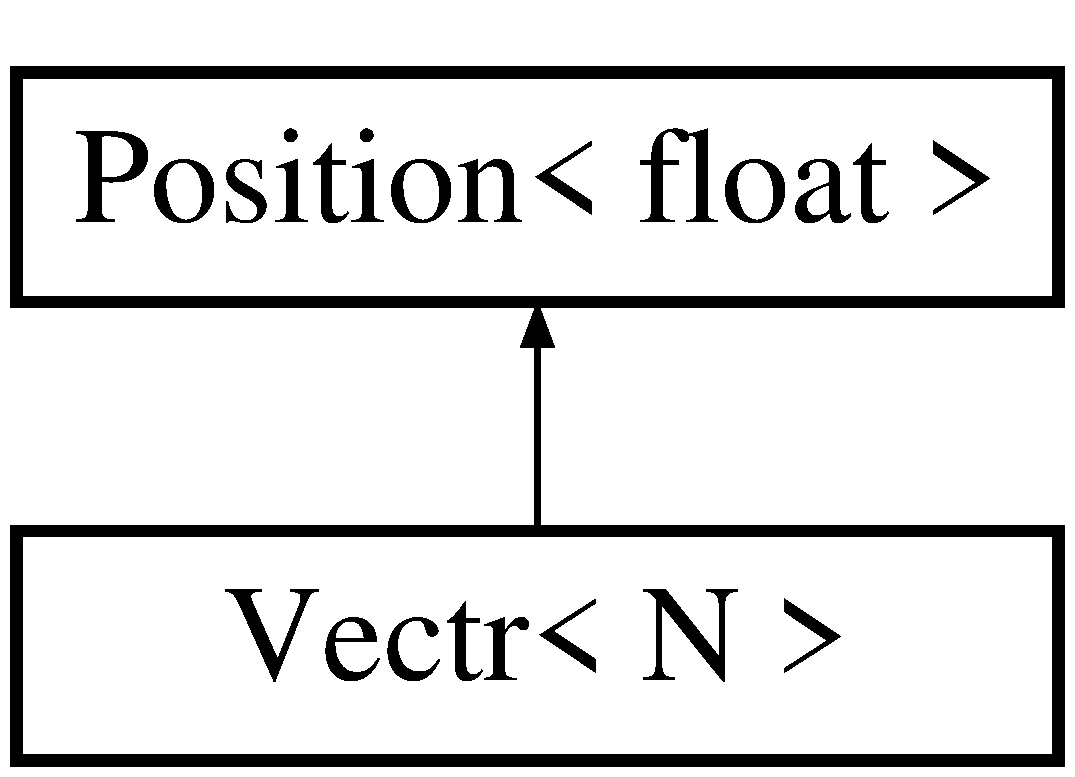
\includegraphics[height=2.000000cm]{struct_vectr}
\end{center}
\end{figure}
\subsection*{Public Member Functions}
\begin{DoxyCompactItemize}
\item 
\hyperlink{struct_vectr_a420d21073da712360069e09ae8053375}{Vectr} ()
\item 
\hyperlink{struct_vectr_ad66fbd7bd3c07f5dbbc3219fe55b38a1}{Vectr} (float heading\-X, float heading\-Y, float heading\-Z, bool monitor\-Velocity)
\item 
\hyperlink{struct_vectr_a9be0609df512b225181c555f1c9adecb}{Vectr} (float heading\-X, float heading\-Y, float heading\-Z, \hyperlink{struct_position}{Position}$<$ N $>$ $\ast$current\-\_\-, bool monitor\-Velocity)
\item 
\hyperlink{struct_vectr_a70f3b6c158dc21d03cb449093126b939}{Vectr} (const \hyperlink{struct_position}{Position}$<$ N $>$ \&most\-Recent\-\_\-, \hyperlink{struct_position}{Position}$<$ N $>$ $\ast$current\-\_\-, bool monitor\-Velocity)
\item 
\hyperlink{struct_vectr_a80e5b2b4bafb5689b82bdf5d87cc4b49}{Vectr} (const \hyperlink{struct_position}{Position}$<$ N $>$ $\ast$current\-\_\-, bool monitor\-Velocity)
\item 
\hyperlink{struct_vectr_a8328879b18c117c7b262ce53f5f1acb2}{Vectr} (const \hyperlink{struct_vectr}{Vectr}$<$ N $>$ \&other)
\item 
\hyperlink{struct_vectr_abf42e2cb15d0406f24c5901dbf0a07e1}{Vectr} (const \hyperlink{struct_vectr}{Vectr}$<$ N $>$ \&other, bool monitor\-Velocity)
\item 
\hyperlink{struct_vectr_a394981732ad6d227e5fe1f25f783ce99}{Vectr} (\hyperlink{struct_vectr}{Vectr}$<$ N $>$ \&\&other)
\item 
\hyperlink{struct_vectr_affbf285f9295dd163cc8b0364b871ade}{$\sim$\-Vectr} ()
\item 
\hyperlink{struct_vectr}{Vectr} \& \hyperlink{struct_vectr_ac2e10f418e5b70d4a48bdfad9bf882c4}{operator=} (const \hyperlink{struct_vectr}{Vectr}$<$ N $>$ \&rhs)
\item 
\hyperlink{struct_vectr}{Vectr} \& \hyperlink{struct_vectr_a94436033bb9fb7e6e970028e91dac958}{operator=} (\hyperlink{struct_vectr}{Vectr}$<$ N $>$ \&\&rhs)
\item 
\hyperlink{struct_vectr}{Vectr} \hyperlink{struct_vectr_a90b87763e1858fdaf27cbcd3b8758d0c}{copy\-Vect} (bool copy\-Velocity) const 
\item 
\hyperlink{struct_velocity}{Velocity}$<$ N $>$ $\ast$ \hyperlink{struct_vectr_a5dc06bff7605656f5d5294db219339b6}{get\-Velocity} ()
\item 
const \hyperlink{struct_position}{Position} $\ast$ \hyperlink{struct_vectr_a0acef7840c315ea742390f8b96d6c782}{get\-Current} () const 
\item 
const \hyperlink{struct_position}{Position} \hyperlink{struct_vectr_a96b306b6f36bc82f9dd68633f3d3568f}{get\-Last} () const 
\item 
void \hyperlink{struct_vectr_aa8638eb9a06d4947a77f800b501e74f0}{normalize} ()
\item 
void \hyperlink{struct_vectr_a94b119ab4adb045161a80a5278dbe0f1}{update\-And\-Normalize} ()
\item 
N \hyperlink{struct_vectr_ae4c3aa958a6d74d96ff119e63c3ae6ea}{get\-Last\-Move\-Distance} ()
\item 
\hyperlink{struct_velocity}{Velocity}$<$ N $>$ \& \hyperlink{struct_vectr_a8ef008609006c8cd2afa56abac2bbe25}{calculate\-Velocity} ()
\end{DoxyCompactItemize}
\subsection*{Static Public Member Functions}
\begin{DoxyCompactItemize}
\item 
static \hyperlink{struct_position}{Position}$<$ N $>$ \hyperlink{struct_vectr_ad293e3f67a0483060d69b4de5dcfe5d2}{calculate\-Next\-Position} (\hyperlink{struct_vectr}{Vectr}$<$ N $>$ \&, float modifier=1.\-0)
\item 
static \hyperlink{struct_position}{Position}$<$ N $>$ \hyperlink{struct_vectr_ac4d91db7639f1f74ba2492aaed2eb01d}{calculate\-Next\-Position\-Checked} (\hyperlink{struct_vectr}{Vectr}$<$ N $>$ \&, float modifier=1.\-0, const \hyperlink{struct_bounds_check}{Bounds\-Check}$<$ N $>$ \&=\hyperlink{struct_bounds_check}{Bounds\-Check}$<$ N $>$\-::default\-Check)
\item 
static \hyperlink{struct_position}{Position}$<$ N $>$ \hyperlink{struct_vectr_abeef5f4dfbd11b7c6bf40779cc191c0e}{calculate\-Reverse\-Next\-Position} (\hyperlink{struct_vectr}{Vectr}$<$ N $>$ \&, float modifier=1.\-0, const \hyperlink{struct_bounds_check}{Bounds\-Check}$<$ N $>$ \&=\hyperlink{struct_bounds_check}{Bounds\-Check}$<$ N $>$\-::default\-Check)
\item 
static \hyperlink{struct_position}{Position}$<$ N $>$ \hyperlink{struct_vectr_a7c8cfdf413bb152bcea5d14017220759}{calculate\-Reverse\-X\-Position} (\hyperlink{struct_vectr}{Vectr}$<$ N $>$ \&, float modifier=1.\-0, const \hyperlink{struct_bounds_check}{Bounds\-Check}$<$ N $>$ \&=\hyperlink{struct_bounds_check}{Bounds\-Check}$<$ N $>$\-::default\-Check)
\item 
static \hyperlink{struct_position}{Position}$<$ N $>$ \hyperlink{struct_vectr_ab897fda165e543696ecdc622af191698}{calculate\-Reverse\-Y\-Position} (\hyperlink{struct_vectr}{Vectr}$<$ N $>$ \&, float modifier=1.\-0, const \hyperlink{struct_bounds_check}{Bounds\-Check}$<$ N $>$ \&=\hyperlink{struct_bounds_check}{Bounds\-Check}$<$ N $>$\-::default\-Check)
\end{DoxyCompactItemize}
\subsection*{Protected Member Functions}
\begin{DoxyCompactItemize}
\item 
\hyperlink{struct_vectr_ae04cf340dddfe1cd05c8dec90e34dd4a}{Vectr} (const \hyperlink{struct_position}{Position}$<$ float $>$ \&override\-Curr\-Data, const \hyperlink{struct_position}{Position}$<$ N $>$ $\ast$current\-\_\-, bool monitor\-Velocity)
\item 
void \hyperlink{struct_vectr_a072798a344fe237c3456f1e962f18672}{update} ()
\end{DoxyCompactItemize}
\subsection*{Protected Attributes}
\begin{DoxyCompactItemize}
\item 
\hyperlink{struct_position}{Position}$<$ N $>$ \hyperlink{struct_vectr_a42723f75b3084b9285cbd205388ba90e}{last}
\item 
\hyperlink{struct_position}{Position}$<$ N $>$ \hyperlink{struct_vectr_a1ef69f90f664d37b4281a02d12b08693}{most\-Recent}
\item 
const \hyperlink{struct_position}{Position}$<$ N $>$ $\ast$ \hyperlink{struct_vectr_ae3215bf0713f2bb9a40f60c0215b4b83}{current}
\item 
N \hyperlink{struct_vectr_a4634576eedac8a5b4651991e0c1f0d4d}{abs\-Distance\-Moved} = 0
\item 
N $\ast$ \hyperlink{struct_vectr_a577bdf47f67b34585ee08696679b2232}{total\-Distance\-Moved}
\item 
\hyperlink{struct_velocity}{Velocity}$<$ N $>$ $\ast$ \hyperlink{struct_vectr_aef611170eac7b1341ff345b9bb108eb7}{velocity}
\item 
bool \hyperlink{struct_vectr_a2dc13bbf566571029a2069a87d165b30}{shared\-Vel\-Bool} = true
\end{DoxyCompactItemize}
\subsection*{Static Protected Attributes}
\begin{DoxyCompactItemize}
\item 
static \hyperlink{class_basic_mutex}{Basic\-Mutex} $\ast$ \hyperlink{struct_vectr_a1cc9dc723075fb24116b6a78ac73e786}{shared\-Vel\-Mutex} = \hyperlink{struct_velocity}{Velocity}$<$N$>$\-::shared\-Vel\-Mutex
\end{DoxyCompactItemize}


\subsection{Detailed Description}
\subsubsection*{template$<$typename N$>$struct Vectr$<$ N $>$}

This class provides facilities for calculating an object's current trajectory, predicting its next \hyperlink{struct_position}{Position}, monitoring its speed, maintaining a record of its last two Positions (for more detailed record keeping of past Positions, see \hyperlink{struct_pos2}{Pos2}), and more.

Note\-: do not use with unsigned ints 

Definition at line 995 of file Position.\-hpp.



\subsection{Constructor \& Destructor Documentation}
\hypertarget{struct_vectr_ae04cf340dddfe1cd05c8dec90e34dd4a}{\index{Vectr@{Vectr}!Vectr@{Vectr}}
\index{Vectr@{Vectr}!Vectr@{Vectr}}
\subsubsection[{Vectr}]{\setlength{\rightskip}{0pt plus 5cm}template$<$typename N$>$ {\bf Vectr}$<$ N $>$\-::{\bf Vectr} (
\begin{DoxyParamCaption}
\item[{const {\bf Position}$<$ float $>$ \&}]{override\-Curr\-Data, }
\item[{const {\bf Position}$<$ N $>$ $\ast$}]{current\-\_\-, }
\item[{bool}]{monitor\-Velocity}
\end{DoxyParamCaption}
)\hspace{0.3cm}{\ttfamily [protected]}}}\label{struct_vectr_ae04cf340dddfe1cd05c8dec90e34dd4a}


Definition at line 1123 of file Position.\-hpp.

\hypertarget{struct_vectr_a420d21073da712360069e09ae8053375}{\index{Vectr@{Vectr}!Vectr@{Vectr}}
\index{Vectr@{Vectr}!Vectr@{Vectr}}
\subsubsection[{Vectr}]{\setlength{\rightskip}{0pt plus 5cm}template$<$typename N$>$ {\bf Vectr}$<$ N $>$\-::{\bf Vectr} (
\begin{DoxyParamCaption}
{}
\end{DoxyParamCaption}
)}}\label{struct_vectr_a420d21073da712360069e09ae8053375}


Definition at line 1088 of file Position.\-hpp.

\hypertarget{struct_vectr_ad66fbd7bd3c07f5dbbc3219fe55b38a1}{\index{Vectr@{Vectr}!Vectr@{Vectr}}
\index{Vectr@{Vectr}!Vectr@{Vectr}}
\subsubsection[{Vectr}]{\setlength{\rightskip}{0pt plus 5cm}template$<$typename N$>$ {\bf Vectr}$<$ N $>$\-::{\bf Vectr} (
\begin{DoxyParamCaption}
\item[{float}]{heading\-X, }
\item[{float}]{heading\-Y, }
\item[{float}]{heading\-Z, }
\item[{bool}]{monitor\-Velocity}
\end{DoxyParamCaption}
)}}\label{struct_vectr_ad66fbd7bd3c07f5dbbc3219fe55b38a1}


Definition at line 1095 of file Position.\-hpp.

\hypertarget{struct_vectr_a9be0609df512b225181c555f1c9adecb}{\index{Vectr@{Vectr}!Vectr@{Vectr}}
\index{Vectr@{Vectr}!Vectr@{Vectr}}
\subsubsection[{Vectr}]{\setlength{\rightskip}{0pt plus 5cm}template$<$typename N$>$ {\bf Vectr}$<$ N $>$\-::{\bf Vectr} (
\begin{DoxyParamCaption}
\item[{float}]{heading\-X, }
\item[{float}]{heading\-Y, }
\item[{float}]{heading\-Z, }
\item[{{\bf Position}$<$ N $>$ $\ast$}]{current\-\_\-, }
\item[{bool}]{monitor\-Velocity}
\end{DoxyParamCaption}
)}}\label{struct_vectr_a9be0609df512b225181c555f1c9adecb}


Definition at line 1109 of file Position.\-hpp.

\hypertarget{struct_vectr_a70f3b6c158dc21d03cb449093126b939}{\index{Vectr@{Vectr}!Vectr@{Vectr}}
\index{Vectr@{Vectr}!Vectr@{Vectr}}
\subsubsection[{Vectr}]{\setlength{\rightskip}{0pt plus 5cm}template$<$typename N$>$ {\bf Vectr}$<$ N $>$\-::{\bf Vectr} (
\begin{DoxyParamCaption}
\item[{const {\bf Position}$<$ N $>$ \&}]{most\-Recent\-\_\-, }
\item[{{\bf Position}$<$ N $>$ $\ast$}]{current\-\_\-, }
\item[{bool}]{monitor\-Velocity}
\end{DoxyParamCaption}
)}}\label{struct_vectr_a70f3b6c158dc21d03cb449093126b939}
\hypertarget{struct_vectr_a80e5b2b4bafb5689b82bdf5d87cc4b49}{\index{Vectr@{Vectr}!Vectr@{Vectr}}
\index{Vectr@{Vectr}!Vectr@{Vectr}}
\subsubsection[{Vectr}]{\setlength{\rightskip}{0pt plus 5cm}template$<$typename N$>$ {\bf Vectr}$<$ N $>$\-::{\bf Vectr} (
\begin{DoxyParamCaption}
\item[{const {\bf Position}$<$ N $>$ $\ast$}]{current\-\_\-, }
\item[{bool}]{monitor\-Velocity}
\end{DoxyParamCaption}
)}}\label{struct_vectr_a80e5b2b4bafb5689b82bdf5d87cc4b49}


Definition at line 1138 of file Position.\-hpp.

\hypertarget{struct_vectr_a8328879b18c117c7b262ce53f5f1acb2}{\index{Vectr@{Vectr}!Vectr@{Vectr}}
\index{Vectr@{Vectr}!Vectr@{Vectr}}
\subsubsection[{Vectr}]{\setlength{\rightskip}{0pt plus 5cm}template$<$typename N$>$ {\bf Vectr}$<$ N $>$\-::{\bf Vectr} (
\begin{DoxyParamCaption}
\item[{const {\bf Vectr}$<$ N $>$ \&}]{other}
\end{DoxyParamCaption}
)}}\label{struct_vectr_a8328879b18c117c7b262ce53f5f1acb2}


Definition at line 1154 of file Position.\-hpp.

\hypertarget{struct_vectr_abf42e2cb15d0406f24c5901dbf0a07e1}{\index{Vectr@{Vectr}!Vectr@{Vectr}}
\index{Vectr@{Vectr}!Vectr@{Vectr}}
\subsubsection[{Vectr}]{\setlength{\rightskip}{0pt plus 5cm}template$<$typename N$>$ {\bf Vectr}$<$ N $>$\-::{\bf Vectr} (
\begin{DoxyParamCaption}
\item[{const {\bf Vectr}$<$ N $>$ \&}]{other, }
\item[{bool}]{monitor\-Velocity}
\end{DoxyParamCaption}
)}}\label{struct_vectr_abf42e2cb15d0406f24c5901dbf0a07e1}


Definition at line 1170 of file Position.\-hpp.

\hypertarget{struct_vectr_a394981732ad6d227e5fe1f25f783ce99}{\index{Vectr@{Vectr}!Vectr@{Vectr}}
\index{Vectr@{Vectr}!Vectr@{Vectr}}
\subsubsection[{Vectr}]{\setlength{\rightskip}{0pt plus 5cm}template$<$typename N$>$ {\bf Vectr}$<$ N $>$\-::{\bf Vectr} (
\begin{DoxyParamCaption}
\item[{{\bf Vectr}$<$ N $>$ \&\&}]{other}
\end{DoxyParamCaption}
)}}\label{struct_vectr_a394981732ad6d227e5fe1f25f783ce99}


Definition at line 1187 of file Position.\-hpp.

\hypertarget{struct_vectr_affbf285f9295dd163cc8b0364b871ade}{\index{Vectr@{Vectr}!$\sim$\-Vectr@{$\sim$\-Vectr}}
\index{$\sim$\-Vectr@{$\sim$\-Vectr}!Vectr@{Vectr}}
\subsubsection[{$\sim$\-Vectr}]{\setlength{\rightskip}{0pt plus 5cm}template$<$typename N $>$ {\bf Vectr}$<$ N $>$\-::$\sim${\bf Vectr} (
\begin{DoxyParamCaption}
{}
\end{DoxyParamCaption}
)}}\label{struct_vectr_affbf285f9295dd163cc8b0364b871ade}


Definition at line 1201 of file Position.\-hpp.



\subsection{Member Function Documentation}
\hypertarget{struct_vectr_ad293e3f67a0483060d69b4de5dcfe5d2}{\index{Vectr@{Vectr}!calculate\-Next\-Position@{calculate\-Next\-Position}}
\index{calculate\-Next\-Position@{calculate\-Next\-Position}!Vectr@{Vectr}}
\subsubsection[{calculate\-Next\-Position}]{\setlength{\rightskip}{0pt plus 5cm}template$<$typename N$>$ {\bf Position}$<$ N $>$ {\bf Vectr}$<$ N $>$\-::calculate\-Next\-Position (
\begin{DoxyParamCaption}
\item[{{\bf Vectr}$<$ N $>$ \&}]{vec, }
\item[{float}]{modifier = {\ttfamily 1.0}}
\end{DoxyParamCaption}
)\hspace{0.3cm}{\ttfamily [static]}}}\label{struct_vectr_ad293e3f67a0483060d69b4de5dcfe5d2}


Definition at line 1355 of file Position.\-hpp.

\hypertarget{struct_vectr_ac4d91db7639f1f74ba2492aaed2eb01d}{\index{Vectr@{Vectr}!calculate\-Next\-Position\-Checked@{calculate\-Next\-Position\-Checked}}
\index{calculate\-Next\-Position\-Checked@{calculate\-Next\-Position\-Checked}!Vectr@{Vectr}}
\subsubsection[{calculate\-Next\-Position\-Checked}]{\setlength{\rightskip}{0pt plus 5cm}template$<$typename N$>$ {\bf Position}$<$ N $>$ {\bf Vectr}$<$ N $>$\-::calculate\-Next\-Position\-Checked (
\begin{DoxyParamCaption}
\item[{{\bf Vectr}$<$ N $>$ \&}]{vec, }
\item[{float}]{modifier = {\ttfamily 1.0}, }
\item[{const {\bf Bounds\-Check}$<$ N $>$ \&}]{check = {\ttfamily {\bf Bounds\-Check}$<$N$>$\-:\-:defaultCheck}}
\end{DoxyParamCaption}
)\hspace{0.3cm}{\ttfamily [static]}}}\label{struct_vectr_ac4d91db7639f1f74ba2492aaed2eb01d}


Definition at line 1374 of file Position.\-hpp.

\hypertarget{struct_vectr_abeef5f4dfbd11b7c6bf40779cc191c0e}{\index{Vectr@{Vectr}!calculate\-Reverse\-Next\-Position@{calculate\-Reverse\-Next\-Position}}
\index{calculate\-Reverse\-Next\-Position@{calculate\-Reverse\-Next\-Position}!Vectr@{Vectr}}
\subsubsection[{calculate\-Reverse\-Next\-Position}]{\setlength{\rightskip}{0pt plus 5cm}template$<$typename N$>$ {\bf Position}$<$ N $>$ {\bf Vectr}$<$ N $>$\-::calculate\-Reverse\-Next\-Position (
\begin{DoxyParamCaption}
\item[{{\bf Vectr}$<$ N $>$ \&}]{vec, }
\item[{float}]{modifier = {\ttfamily 1.0}, }
\item[{const {\bf Bounds\-Check}$<$ N $>$ \&}]{check = {\ttfamily {\bf Bounds\-Check}$<$N$>$\-:\-:defaultCheck}}
\end{DoxyParamCaption}
)\hspace{0.3cm}{\ttfamily [static]}}}\label{struct_vectr_abeef5f4dfbd11b7c6bf40779cc191c0e}


Definition at line 1393 of file Position.\-hpp.

\hypertarget{struct_vectr_a7c8cfdf413bb152bcea5d14017220759}{\index{Vectr@{Vectr}!calculate\-Reverse\-X\-Position@{calculate\-Reverse\-X\-Position}}
\index{calculate\-Reverse\-X\-Position@{calculate\-Reverse\-X\-Position}!Vectr@{Vectr}}
\subsubsection[{calculate\-Reverse\-X\-Position}]{\setlength{\rightskip}{0pt plus 5cm}template$<$typename N$>$ {\bf Position}$<$ N $>$ {\bf Vectr}$<$ N $>$\-::calculate\-Reverse\-X\-Position (
\begin{DoxyParamCaption}
\item[{{\bf Vectr}$<$ N $>$ \&}]{vec, }
\item[{float}]{modifier = {\ttfamily 1.0}, }
\item[{const {\bf Bounds\-Check}$<$ N $>$ \&}]{check = {\ttfamily {\bf Bounds\-Check}$<$N$>$\-:\-:defaultCheck}}
\end{DoxyParamCaption}
)\hspace{0.3cm}{\ttfamily [static]}}}\label{struct_vectr_a7c8cfdf413bb152bcea5d14017220759}


Definition at line 1401 of file Position.\-hpp.

\hypertarget{struct_vectr_ab897fda165e543696ecdc622af191698}{\index{Vectr@{Vectr}!calculate\-Reverse\-Y\-Position@{calculate\-Reverse\-Y\-Position}}
\index{calculate\-Reverse\-Y\-Position@{calculate\-Reverse\-Y\-Position}!Vectr@{Vectr}}
\subsubsection[{calculate\-Reverse\-Y\-Position}]{\setlength{\rightskip}{0pt plus 5cm}template$<$typename N$>$ {\bf Position}$<$ N $>$ {\bf Vectr}$<$ N $>$\-::calculate\-Reverse\-Y\-Position (
\begin{DoxyParamCaption}
\item[{{\bf Vectr}$<$ N $>$ \&}]{vec, }
\item[{float}]{modifier = {\ttfamily 1.0}, }
\item[{const {\bf Bounds\-Check}$<$ N $>$ \&}]{check = {\ttfamily {\bf Bounds\-Check}$<$N$>$\-:\-:defaultCheck}}
\end{DoxyParamCaption}
)\hspace{0.3cm}{\ttfamily [static]}}}\label{struct_vectr_ab897fda165e543696ecdc622af191698}


Definition at line 1407 of file Position.\-hpp.

\hypertarget{struct_vectr_a8ef008609006c8cd2afa56abac2bbe25}{\index{Vectr@{Vectr}!calculate\-Velocity@{calculate\-Velocity}}
\index{calculate\-Velocity@{calculate\-Velocity}!Vectr@{Vectr}}
\subsubsection[{calculate\-Velocity}]{\setlength{\rightskip}{0pt plus 5cm}template$<$typename N $>$ {\bf Velocity}$<$ N $>$ \& {\bf Vectr}$<$ N $>$\-::calculate\-Velocity (
\begin{DoxyParamCaption}
{}
\end{DoxyParamCaption}
)}}\label{struct_vectr_a8ef008609006c8cd2afa56abac2bbe25}


Definition at line 1350 of file Position.\-hpp.

\hypertarget{struct_vectr_a90b87763e1858fdaf27cbcd3b8758d0c}{\index{Vectr@{Vectr}!copy\-Vect@{copy\-Vect}}
\index{copy\-Vect@{copy\-Vect}!Vectr@{Vectr}}
\subsubsection[{copy\-Vect}]{\setlength{\rightskip}{0pt plus 5cm}template$<$typename N $>$ {\bf Vectr}$<$ N $>$ {\bf Vectr}$<$ N $>$\-::copy\-Vect (
\begin{DoxyParamCaption}
\item[{bool}]{copy\-Velocity}
\end{DoxyParamCaption}
) const}}\label{struct_vectr_a90b87763e1858fdaf27cbcd3b8758d0c}


Definition at line 1275 of file Position.\-hpp.

\hypertarget{struct_vectr_a0acef7840c315ea742390f8b96d6c782}{\index{Vectr@{Vectr}!get\-Current@{get\-Current}}
\index{get\-Current@{get\-Current}!Vectr@{Vectr}}
\subsubsection[{get\-Current}]{\setlength{\rightskip}{0pt plus 5cm}template$<$typename N$>$ const {\bf Position}$\ast$ {\bf Vectr}$<$ N $>$\-::get\-Current (
\begin{DoxyParamCaption}
{}
\end{DoxyParamCaption}
) const\hspace{0.3cm}{\ttfamily [inline]}}}\label{struct_vectr_a0acef7840c315ea742390f8b96d6c782}


Definition at line 1054 of file Position.\-hpp.

\hypertarget{struct_vectr_a96b306b6f36bc82f9dd68633f3d3568f}{\index{Vectr@{Vectr}!get\-Last@{get\-Last}}
\index{get\-Last@{get\-Last}!Vectr@{Vectr}}
\subsubsection[{get\-Last}]{\setlength{\rightskip}{0pt plus 5cm}template$<$typename N$>$ const {\bf Position} {\bf Vectr}$<$ N $>$\-::get\-Last (
\begin{DoxyParamCaption}
{}
\end{DoxyParamCaption}
) const\hspace{0.3cm}{\ttfamily [inline]}}}\label{struct_vectr_a96b306b6f36bc82f9dd68633f3d3568f}


Definition at line 1056 of file Position.\-hpp.

\hypertarget{struct_vectr_ae4c3aa958a6d74d96ff119e63c3ae6ea}{\index{Vectr@{Vectr}!get\-Last\-Move\-Distance@{get\-Last\-Move\-Distance}}
\index{get\-Last\-Move\-Distance@{get\-Last\-Move\-Distance}!Vectr@{Vectr}}
\subsubsection[{get\-Last\-Move\-Distance}]{\setlength{\rightskip}{0pt plus 5cm}template$<$typename N$>$ N {\bf Vectr}$<$ N $>$\-::get\-Last\-Move\-Distance (
\begin{DoxyParamCaption}
{}
\end{DoxyParamCaption}
)\hspace{0.3cm}{\ttfamily [inline]}}}\label{struct_vectr_ae4c3aa958a6d74d96ff119e63c3ae6ea}


Definition at line 1062 of file Position.\-hpp.

\hypertarget{struct_vectr_a5dc06bff7605656f5d5294db219339b6}{\index{Vectr@{Vectr}!get\-Velocity@{get\-Velocity}}
\index{get\-Velocity@{get\-Velocity}!Vectr@{Vectr}}
\subsubsection[{get\-Velocity}]{\setlength{\rightskip}{0pt plus 5cm}template$<$typename N$>$ {\bf Velocity}$<$N$>$$\ast$ {\bf Vectr}$<$ N $>$\-::get\-Velocity (
\begin{DoxyParamCaption}
{}
\end{DoxyParamCaption}
)\hspace{0.3cm}{\ttfamily [inline]}}}\label{struct_vectr_a5dc06bff7605656f5d5294db219339b6}


Definition at line 1052 of file Position.\-hpp.

\hypertarget{struct_vectr_aa8638eb9a06d4947a77f800b501e74f0}{\index{Vectr@{Vectr}!normalize@{normalize}}
\index{normalize@{normalize}!Vectr@{Vectr}}
\subsubsection[{normalize}]{\setlength{\rightskip}{0pt plus 5cm}template$<$typename N $>$ void {\bf Vectr}$<$ N $>$\-::normalize (
\begin{DoxyParamCaption}
{}
\end{DoxyParamCaption}
)}}\label{struct_vectr_aa8638eb9a06d4947a77f800b501e74f0}


Definition at line 1332 of file Position.\-hpp.

\hypertarget{struct_vectr_ac2e10f418e5b70d4a48bdfad9bf882c4}{\index{Vectr@{Vectr}!operator=@{operator=}}
\index{operator=@{operator=}!Vectr@{Vectr}}
\subsubsection[{operator=}]{\setlength{\rightskip}{0pt plus 5cm}template$<$typename N$>$ {\bf Vectr}$<$ N $>$ \& {\bf Vectr}$<$ N $>$\-::operator= (
\begin{DoxyParamCaption}
\item[{const {\bf Vectr}$<$ N $>$ \&}]{rhs}
\end{DoxyParamCaption}
)}}\label{struct_vectr_ac2e10f418e5b70d4a48bdfad9bf882c4}


Definition at line 1226 of file Position.\-hpp.

\hypertarget{struct_vectr_a94436033bb9fb7e6e970028e91dac958}{\index{Vectr@{Vectr}!operator=@{operator=}}
\index{operator=@{operator=}!Vectr@{Vectr}}
\subsubsection[{operator=}]{\setlength{\rightskip}{0pt plus 5cm}template$<$typename N$>$ {\bf Vectr}$<$ N $>$ \& {\bf Vectr}$<$ N $>$\-::operator= (
\begin{DoxyParamCaption}
\item[{{\bf Vectr}$<$ N $>$ \&\&}]{rhs}
\end{DoxyParamCaption}
)}}\label{struct_vectr_a94436033bb9fb7e6e970028e91dac958}


Definition at line 1256 of file Position.\-hpp.

\hypertarget{struct_vectr_a072798a344fe237c3456f1e962f18672}{\index{Vectr@{Vectr}!update@{update}}
\index{update@{update}!Vectr@{Vectr}}
\subsubsection[{update}]{\setlength{\rightskip}{0pt plus 5cm}template$<$typename N $>$ void {\bf Vectr}$<$ N $>$\-::update (
\begin{DoxyParamCaption}
{}
\end{DoxyParamCaption}
)\hspace{0.3cm}{\ttfamily [protected]}}}\label{struct_vectr_a072798a344fe237c3456f1e962f18672}


Definition at line 1314 of file Position.\-hpp.

\hypertarget{struct_vectr_a94b119ab4adb045161a80a5278dbe0f1}{\index{Vectr@{Vectr}!update\-And\-Normalize@{update\-And\-Normalize}}
\index{update\-And\-Normalize@{update\-And\-Normalize}!Vectr@{Vectr}}
\subsubsection[{update\-And\-Normalize}]{\setlength{\rightskip}{0pt plus 5cm}template$<$typename N $>$ void {\bf Vectr}$<$ N $>$\-::update\-And\-Normalize (
\begin{DoxyParamCaption}
{}
\end{DoxyParamCaption}
)}}\label{struct_vectr_a94b119ab4adb045161a80a5278dbe0f1}


Definition at line 1344 of file Position.\-hpp.



\subsection{Member Data Documentation}
\hypertarget{struct_vectr_a4634576eedac8a5b4651991e0c1f0d4d}{\index{Vectr@{Vectr}!abs\-Distance\-Moved@{abs\-Distance\-Moved}}
\index{abs\-Distance\-Moved@{abs\-Distance\-Moved}!Vectr@{Vectr}}
\subsubsection[{abs\-Distance\-Moved}]{\setlength{\rightskip}{0pt plus 5cm}template$<$typename N$>$ N {\bf Vectr}$<$ N $>$\-::abs\-Distance\-Moved = 0\hspace{0.3cm}{\ttfamily [protected]}}}\label{struct_vectr_a4634576eedac8a5b4651991e0c1f0d4d}
The non-\/normalized distance between the current \hyperlink{struct_position}{Position} and most\-Recent \hyperlink{struct_position}{Position} 

Definition at line 1019 of file Position.\-hpp.

\hypertarget{struct_vectr_ae3215bf0713f2bb9a40f60c0215b4b83}{\index{Vectr@{Vectr}!current@{current}}
\index{current@{current}!Vectr@{Vectr}}
\subsubsection[{current}]{\setlength{\rightskip}{0pt plus 5cm}template$<$typename N$>$ const {\bf Position}$<$N$>$$\ast$ {\bf Vectr}$<$ N $>$\-::current\hspace{0.3cm}{\ttfamily [protected]}}}\label{struct_vectr_ae3215bf0713f2bb9a40f60c0215b4b83}
A pointer to the current \hyperlink{struct_position}{Position} 

Definition at line 1014 of file Position.\-hpp.

\hypertarget{struct_vectr_a42723f75b3084b9285cbd205388ba90e}{\index{Vectr@{Vectr}!last@{last}}
\index{last@{last}!Vectr@{Vectr}}
\subsubsection[{last}]{\setlength{\rightskip}{0pt plus 5cm}template$<$typename N$>$ {\bf Position}$<$N$>$ {\bf Vectr}$<$ N $>$\-::last\hspace{0.3cm}{\ttfamily [protected]}}}\label{struct_vectr_a42723f75b3084b9285cbd205388ba90e}
The \hyperlink{struct_position}{Position} preceding the most recent \hyperlink{struct_position}{Position} 

Definition at line 1004 of file Position.\-hpp.

\hypertarget{struct_vectr_a1ef69f90f664d37b4281a02d12b08693}{\index{Vectr@{Vectr}!most\-Recent@{most\-Recent}}
\index{most\-Recent@{most\-Recent}!Vectr@{Vectr}}
\subsubsection[{most\-Recent}]{\setlength{\rightskip}{0pt plus 5cm}template$<$typename N$>$ {\bf Position}$<$N$>$ {\bf Vectr}$<$ N $>$\-::most\-Recent\hspace{0.3cm}{\ttfamily [protected]}}}\label{struct_vectr_a1ef69f90f664d37b4281a02d12b08693}
The \hyperlink{struct_position}{Position} most recently visited 

Definition at line 1009 of file Position.\-hpp.

\hypertarget{struct_vectr_a2dc13bbf566571029a2069a87d165b30}{\index{Vectr@{Vectr}!shared\-Vel\-Bool@{shared\-Vel\-Bool}}
\index{shared\-Vel\-Bool@{shared\-Vel\-Bool}!Vectr@{Vectr}}
\subsubsection[{shared\-Vel\-Bool}]{\setlength{\rightskip}{0pt plus 5cm}template$<$typename N$>$ bool {\bf Vectr}$<$ N $>$\-::shared\-Vel\-Bool = true\hspace{0.3cm}{\ttfamily [protected]}}}\label{struct_vectr_a2dc13bbf566571029a2069a87d165b30}


Definition at line 1029 of file Position.\-hpp.

\hypertarget{struct_vectr_a1cc9dc723075fb24116b6a78ac73e786}{\index{Vectr@{Vectr}!shared\-Vel\-Mutex@{shared\-Vel\-Mutex}}
\index{shared\-Vel\-Mutex@{shared\-Vel\-Mutex}!Vectr@{Vectr}}
\subsubsection[{shared\-Vel\-Mutex}]{\setlength{\rightskip}{0pt plus 5cm}template$<$typename N$>$ {\bf Basic\-Mutex} $\ast$ {\bf Vectr}$<$ N $>$\-::shared\-Vel\-Mutex = {\bf Velocity}$<$N$>$\-::shared\-Vel\-Mutex\hspace{0.3cm}{\ttfamily [static]}, {\ttfamily [protected]}}}\label{struct_vectr_a1cc9dc723075fb24116b6a78ac73e786}


Definition at line 999 of file Position.\-hpp.

\hypertarget{struct_vectr_a577bdf47f67b34585ee08696679b2232}{\index{Vectr@{Vectr}!total\-Distance\-Moved@{total\-Distance\-Moved}}
\index{total\-Distance\-Moved@{total\-Distance\-Moved}!Vectr@{Vectr}}
\subsubsection[{total\-Distance\-Moved}]{\setlength{\rightskip}{0pt plus 5cm}template$<$typename N$>$ N$\ast$ {\bf Vectr}$<$ N $>$\-::total\-Distance\-Moved\hspace{0.3cm}{\ttfamily [protected]}}}\label{struct_vectr_a577bdf47f67b34585ee08696679b2232}


Definition at line 1021 of file Position.\-hpp.

\hypertarget{struct_vectr_aef611170eac7b1341ff345b9bb108eb7}{\index{Vectr@{Vectr}!velocity@{velocity}}
\index{velocity@{velocity}!Vectr@{Vectr}}
\subsubsection[{velocity}]{\setlength{\rightskip}{0pt plus 5cm}template$<$typename N$>$ {\bf Velocity}$<$N$>$$\ast$ {\bf Vectr}$<$ N $>$\-::velocity\hspace{0.3cm}{\ttfamily [protected]}}}\label{struct_vectr_aef611170eac7b1341ff345b9bb108eb7}
Monitors velocity 

Definition at line 1026 of file Position.\-hpp.



The documentation for this struct was generated from the following file\-:\begin{DoxyCompactItemize}
\item 
/\-Volumes/\-O\-S X H\-D\-D/\-Users/\-Adam/\-Developer/\-Sprite\-Fight/\-Util/\hyperlink{_position_8hpp}{Position.\-hpp}\end{DoxyCompactItemize}

\hypertarget{struct_velocity}{\section{Velocity$<$ N $>$ Struct Template Reference}
\label{struct_velocity}\index{Velocity$<$ N $>$@{Velocity$<$ N $>$}}
}


{\ttfamily \#include $<$Velocity.\-hpp$>$}

\subsection*{Public Member Functions}
\begin{DoxyCompactItemize}
\item 
\hyperlink{struct_velocity_a5a7fc681247a544a000718a35c202958}{Velocity} (const \hyperlink{_velocity_8hpp_a29fbe3dd3ce308a36d5b29488daddcaa}{Distance} $\ast$\hyperlink{struct_velocity_a3f3d268a5d9452ad912c19cfcc7c0394}{distance}, mutex $\ast$mut, bool $\ast$\hyperlink{struct_velocity_a099e0c3e044ce52e11b1e7ab225f896c}{local\-Continue\-Signal})
\item 
\hyperlink{struct_velocity_ab501061b7933ea4bf8d722b5e092972a}{Velocity} (const \hyperlink{_velocity_8hpp_a29fbe3dd3ce308a36d5b29488daddcaa}{Distance} $\ast$\hyperlink{struct_velocity_a3f3d268a5d9452ad912c19cfcc7c0394}{distance}, mutex $\ast$mut, bool $\ast$\hyperlink{struct_velocity_a099e0c3e044ce52e11b1e7ab225f896c}{local\-Continue\-Signal}, chrono\-::nanoseconds base\-Time\-Unit\-Override)
\item 
\hyperlink{struct_velocity_a8763237baab85450aeadd2f1df96c6ec}{Velocity} (const \hyperlink{struct_velocity}{Velocity} \&other)=delete
\item 
\hyperlink{struct_velocity_a5311e10fd1ff6dff1656507d5a7d3d19}{Velocity} (\hyperlink{struct_velocity}{Velocity} \&\&other)=delete
\item 
\hyperlink{struct_velocity_a328da698ec2f9cbf0de0ab519b6d7f50}{$\sim$\-Velocity} ()
\item 
\hyperlink{struct_velocity}{Velocity} \& \hyperlink{struct_velocity_a46e6358260ffa948eb21b1e235960e56}{operator=} (const \hyperlink{struct_velocity}{Velocity} \&rhs)=delete
\item 
\hyperlink{struct_velocity}{Velocity} \& \hyperlink{struct_velocity_a0b9ef6d1f184b6012a2dcc3b7a65539e}{operator=} (\hyperlink{struct_velocity}{Velocity} \&\&rhs)=delete
\item 
double \hyperlink{struct_velocity_a39c1fe5e6fc453aa435a648d6ce5ef05}{get\-Value} ()
\end{DoxyCompactItemize}
\subsection*{Static Public Member Functions}
\begin{DoxyCompactItemize}
\item 
static const vector$<$ \hyperlink{struct_velocity}{Velocity} $\ast$ $>$ $\ast$ \hyperlink{struct_velocity_af8c34fb6b57a667c06e7baa1801f5df9}{get\-Velocity\-Storage} ()
\item 
static void \hyperlink{struct_velocity_ab96b02fb83753526f730e2c5b0337a62}{monitor\-Velocity} ()
\end{DoxyCompactItemize}
\subsection*{Static Public Attributes}
\begin{DoxyCompactItemize}
\item 
static \hyperlink{class_basic_mutex}{Basic\-Mutex} $\ast$ \hyperlink{struct_velocity_a68112c2f090288d4921a53a21390eac8}{shared\-Vel\-Mutex} = new \hyperlink{class_basic_mutex}{Basic\-Mutex}()
\end{DoxyCompactItemize}
\subsection*{Static Protected Member Functions}
\begin{DoxyCompactItemize}
\item 
static void \hyperlink{struct_velocity_a7676bfee3f05da2e4ced84c838f0c1c6}{calculate\-Velocity} ()
\end{DoxyCompactItemize}
\subsection*{Protected Attributes}
\begin{DoxyCompactItemize}
\item 
int \hyperlink{struct_velocity_a3f33b62ecfeeeb79c13cd732fbb3a05c}{id}
\item 
const \hyperlink{_velocity_8hpp_a29fbe3dd3ce308a36d5b29488daddcaa}{Distance} $\ast$ \hyperlink{struct_velocity_a3f3d268a5d9452ad912c19cfcc7c0394}{distance}
\item 
\hyperlink{class_timer}{Timer} $\ast$ \hyperlink{struct_velocity_a99f61fd4486ecad5fdbf0c8d3da8c4a0}{timer}
\item 
bool $\ast$ \hyperlink{struct_velocity_a099e0c3e044ce52e11b1e7ab225f896c}{local\-Continue\-Signal}
\item 
\hyperlink{_velocity_8hpp_a29fbe3dd3ce308a36d5b29488daddcaa}{Distance} \hyperlink{struct_velocity_a4a65b272ce588eab6a9a9fa1fdb94a01}{last\-Distance} = 0
\item 
chrono\-::nanoseconds \hyperlink{struct_velocity_a70e2af5664f11aeb266920916c271712}{base\-Time\-Unit} = std\-::chrono\-::milliseconds(30)
\item 
double \hyperlink{struct_velocity_acb312e3b7523314efd771a52fe8f2982}{last\-Velocity} = 0
\end{DoxyCompactItemize}
\subsection*{Static Protected Attributes}
\begin{DoxyCompactItemize}
\item 
static bool \hyperlink{struct_velocity_a014fe36081e4170fc42b605048c6086c}{velocity\-Monitor\-Init} = false
\item 
static unsigned \hyperlink{struct_velocity_a4ebc19cb1b4fc60b609556073a1d8b36}{I\-Ds} = 0
\item 
static vector$<$ \hyperlink{struct_velocity}{Velocity} $\ast$ $>$ \hyperlink{struct_velocity_a3815a4870a3cb81cf239d58e84eb9284}{velocity\-Storage} = vector$<$\hyperlink{struct_velocity}{Velocity}$<$N$>$ $\ast$$>$()
\end{DoxyCompactItemize}


\subsection{Detailed Description}
\subsubsection*{template$<$typename N$>$struct Velocity$<$ N $>$}



Definition at line 32 of file Velocity.\-hpp.



\subsection{Constructor \& Destructor Documentation}
\hypertarget{struct_velocity_a5a7fc681247a544a000718a35c202958}{\index{Velocity@{Velocity}!Velocity@{Velocity}}
\index{Velocity@{Velocity}!Velocity@{Velocity}}
\subsubsection[{Velocity}]{\setlength{\rightskip}{0pt plus 5cm}template$<$typename N$>$ {\bf Velocity}$<$ N $>$\-::{\bf Velocity} (
\begin{DoxyParamCaption}
\item[{const {\bf Distance} $\ast$}]{distance, }
\item[{mutex $\ast$}]{mut, }
\item[{bool $\ast$}]{local\-Continue\-Signal}
\end{DoxyParamCaption}
)\hspace{0.3cm}{\ttfamily [inline]}}}\label{struct_velocity_a5a7fc681247a544a000718a35c202958}
Constructs a \hyperlink{struct_velocity}{Velocity} object. Distance is a pointer that should increase in value as the caller moves. When \hyperlink{struct_velocity}{Velocity} detects that distance has changed from its initial value, it will begin monitoring speed.


\begin{DoxyParams}{Parameters}
{\em distance} & A pointer to the distance covered by the client class, which \hyperlink{struct_velocity}{Velocity} expects to change over time \\
\hline
{\em mut} & A mutex shared with \hyperlink{struct_velocity}{Velocity} that should be locked when this velocity or distance is about to be deleted \\
\hline
\end{DoxyParams}


Definition at line 80 of file Velocity.\-hpp.

\hypertarget{struct_velocity_ab501061b7933ea4bf8d722b5e092972a}{\index{Velocity@{Velocity}!Velocity@{Velocity}}
\index{Velocity@{Velocity}!Velocity@{Velocity}}
\subsubsection[{Velocity}]{\setlength{\rightskip}{0pt plus 5cm}template$<$typename N$>$ {\bf Velocity}$<$ N $>$\-::{\bf Velocity} (
\begin{DoxyParamCaption}
\item[{const {\bf Distance} $\ast$}]{distance, }
\item[{mutex $\ast$}]{mut, }
\item[{bool $\ast$}]{local\-Continue\-Signal, }
\item[{chrono\-::nanoseconds}]{base\-Time\-Unit\-Override}
\end{DoxyParamCaption}
)\hspace{0.3cm}{\ttfamily [inline]}}}\label{struct_velocity_ab501061b7933ea4bf8d722b5e092972a}


Definition at line 97 of file Velocity.\-hpp.

\hypertarget{struct_velocity_a8763237baab85450aeadd2f1df96c6ec}{\index{Velocity@{Velocity}!Velocity@{Velocity}}
\index{Velocity@{Velocity}!Velocity@{Velocity}}
\subsubsection[{Velocity}]{\setlength{\rightskip}{0pt plus 5cm}template$<$typename N$>$ {\bf Velocity}$<$ N $>$\-::{\bf Velocity} (
\begin{DoxyParamCaption}
\item[{const {\bf Velocity}$<$ N $>$ \&}]{other}
\end{DoxyParamCaption}
)\hspace{0.3cm}{\ttfamily [delete]}}}\label{struct_velocity_a8763237baab85450aeadd2f1df96c6ec}
\hypertarget{struct_velocity_a5311e10fd1ff6dff1656507d5a7d3d19}{\index{Velocity@{Velocity}!Velocity@{Velocity}}
\index{Velocity@{Velocity}!Velocity@{Velocity}}
\subsubsection[{Velocity}]{\setlength{\rightskip}{0pt plus 5cm}template$<$typename N$>$ {\bf Velocity}$<$ N $>$\-::{\bf Velocity} (
\begin{DoxyParamCaption}
\item[{{\bf Velocity}$<$ N $>$ \&\&}]{other}
\end{DoxyParamCaption}
)\hspace{0.3cm}{\ttfamily [delete]}}}\label{struct_velocity_a5311e10fd1ff6dff1656507d5a7d3d19}
\hypertarget{struct_velocity_a328da698ec2f9cbf0de0ab519b6d7f50}{\index{Velocity@{Velocity}!$\sim$\-Velocity@{$\sim$\-Velocity}}
\index{$\sim$\-Velocity@{$\sim$\-Velocity}!Velocity@{Velocity}}
\subsubsection[{$\sim$\-Velocity}]{\setlength{\rightskip}{0pt plus 5cm}template$<$typename N$>$ {\bf Velocity}$<$ N $>$\-::$\sim${\bf Velocity} (
\begin{DoxyParamCaption}
{}
\end{DoxyParamCaption}
)\hspace{0.3cm}{\ttfamily [inline]}}}\label{struct_velocity_a328da698ec2f9cbf0de0ab519b6d7f50}


Definition at line 118 of file Velocity.\-hpp.



\subsection{Member Function Documentation}
\hypertarget{struct_velocity_a7676bfee3f05da2e4ced84c838f0c1c6}{\index{Velocity@{Velocity}!calculate\-Velocity@{calculate\-Velocity}}
\index{calculate\-Velocity@{calculate\-Velocity}!Velocity@{Velocity}}
\subsubsection[{calculate\-Velocity}]{\setlength{\rightskip}{0pt plus 5cm}template$<$typename N $>$ void {\bf Velocity}$<$ N $>$\-::calculate\-Velocity (
\begin{DoxyParamCaption}
{}
\end{DoxyParamCaption}
)\hspace{0.3cm}{\ttfamily [static]}, {\ttfamily [protected]}}}\label{struct_velocity_a7676bfee3f05da2e4ced84c838f0c1c6}


Definition at line 170 of file Velocity.\-hpp.

\hypertarget{struct_velocity_a39c1fe5e6fc453aa435a648d6ce5ef05}{\index{Velocity@{Velocity}!get\-Value@{get\-Value}}
\index{get\-Value@{get\-Value}!Velocity@{Velocity}}
\subsubsection[{get\-Value}]{\setlength{\rightskip}{0pt plus 5cm}template$<$typename N$>$ double {\bf Velocity}$<$ N $>$\-::get\-Value (
\begin{DoxyParamCaption}
{}
\end{DoxyParamCaption}
)\hspace{0.3cm}{\ttfamily [inline]}}}\label{struct_velocity_a39c1fe5e6fc453aa435a648d6ce5ef05}


Definition at line 137 of file Velocity.\-hpp.

\hypertarget{struct_velocity_af8c34fb6b57a667c06e7baa1801f5df9}{\index{Velocity@{Velocity}!get\-Velocity\-Storage@{get\-Velocity\-Storage}}
\index{get\-Velocity\-Storage@{get\-Velocity\-Storage}!Velocity@{Velocity}}
\subsubsection[{get\-Velocity\-Storage}]{\setlength{\rightskip}{0pt plus 5cm}template$<$typename N$>$ static const vector$<${\bf Velocity} $\ast$$>$$\ast$ {\bf Velocity}$<$ N $>$\-::get\-Velocity\-Storage (
\begin{DoxyParamCaption}
{}
\end{DoxyParamCaption}
)\hspace{0.3cm}{\ttfamily [inline]}, {\ttfamily [static]}}}\label{struct_velocity_af8c34fb6b57a667c06e7baa1801f5df9}


Definition at line 67 of file Velocity.\-hpp.

\hypertarget{struct_velocity_ab96b02fb83753526f730e2c5b0337a62}{\index{Velocity@{Velocity}!monitor\-Velocity@{monitor\-Velocity}}
\index{monitor\-Velocity@{monitor\-Velocity}!Velocity@{Velocity}}
\subsubsection[{monitor\-Velocity}]{\setlength{\rightskip}{0pt plus 5cm}template$<$typename N $>$ void {\bf Velocity}$<$ N $>$\-::monitor\-Velocity (
\begin{DoxyParamCaption}
{}
\end{DoxyParamCaption}
)\hspace{0.3cm}{\ttfamily [static]}}}\label{struct_velocity_ab96b02fb83753526f730e2c5b0337a62}


Definition at line 156 of file Velocity.\-hpp.

\hypertarget{struct_velocity_a46e6358260ffa948eb21b1e235960e56}{\index{Velocity@{Velocity}!operator=@{operator=}}
\index{operator=@{operator=}!Velocity@{Velocity}}
\subsubsection[{operator=}]{\setlength{\rightskip}{0pt plus 5cm}template$<$typename N$>$ {\bf Velocity}\& {\bf Velocity}$<$ N $>$\-::operator= (
\begin{DoxyParamCaption}
\item[{const {\bf Velocity}$<$ N $>$ \&}]{rhs}
\end{DoxyParamCaption}
)\hspace{0.3cm}{\ttfamily [delete]}}}\label{struct_velocity_a46e6358260ffa948eb21b1e235960e56}
\hypertarget{struct_velocity_a0b9ef6d1f184b6012a2dcc3b7a65539e}{\index{Velocity@{Velocity}!operator=@{operator=}}
\index{operator=@{operator=}!Velocity@{Velocity}}
\subsubsection[{operator=}]{\setlength{\rightskip}{0pt plus 5cm}template$<$typename N$>$ {\bf Velocity}\& {\bf Velocity}$<$ N $>$\-::operator= (
\begin{DoxyParamCaption}
\item[{{\bf Velocity}$<$ N $>$ \&\&}]{rhs}
\end{DoxyParamCaption}
)\hspace{0.3cm}{\ttfamily [delete]}}}\label{struct_velocity_a0b9ef6d1f184b6012a2dcc3b7a65539e}


\subsection{Member Data Documentation}
\hypertarget{struct_velocity_a70e2af5664f11aeb266920916c271712}{\index{Velocity@{Velocity}!base\-Time\-Unit@{base\-Time\-Unit}}
\index{base\-Time\-Unit@{base\-Time\-Unit}!Velocity@{Velocity}}
\subsubsection[{base\-Time\-Unit}]{\setlength{\rightskip}{0pt plus 5cm}template$<$typename N$>$ chrono\-::nanoseconds {\bf Velocity}$<$ N $>$\-::base\-Time\-Unit = std\-::chrono\-::milliseconds(30)\hspace{0.3cm}{\ttfamily [protected]}}}\label{struct_velocity_a70e2af5664f11aeb266920916c271712}
The unit of time that will function as the denominator for this \hyperlink{struct_velocity}{Velocity} object. By default it is 64 milliseconds. 

Definition at line 54 of file Velocity.\-hpp.

\hypertarget{struct_velocity_a3f3d268a5d9452ad912c19cfcc7c0394}{\index{Velocity@{Velocity}!distance@{distance}}
\index{distance@{distance}!Velocity@{Velocity}}
\subsubsection[{distance}]{\setlength{\rightskip}{0pt plus 5cm}template$<$typename N$>$ const {\bf Distance}$\ast$ {\bf Velocity}$<$ N $>$\-::distance\hspace{0.3cm}{\ttfamily [protected]}}}\label{struct_velocity_a3f3d268a5d9452ad912c19cfcc7c0394}


Definition at line 44 of file Velocity.\-hpp.

\hypertarget{struct_velocity_a3f33b62ecfeeeb79c13cd732fbb3a05c}{\index{Velocity@{Velocity}!id@{id}}
\index{id@{id}!Velocity@{Velocity}}
\subsubsection[{id}]{\setlength{\rightskip}{0pt plus 5cm}template$<$typename N$>$ int {\bf Velocity}$<$ N $>$\-::id\hspace{0.3cm}{\ttfamily [protected]}}}\label{struct_velocity_a3f33b62ecfeeeb79c13cd732fbb3a05c}


Definition at line 43 of file Velocity.\-hpp.

\hypertarget{struct_velocity_a4ebc19cb1b4fc60b609556073a1d8b36}{\index{Velocity@{Velocity}!I\-Ds@{I\-Ds}}
\index{I\-Ds@{I\-Ds}!Velocity@{Velocity}}
\subsubsection[{I\-Ds}]{\setlength{\rightskip}{0pt plus 5cm}template$<$typename N$>$ unsigned {\bf Velocity}$<$ N $>$\-::I\-Ds = 0\hspace{0.3cm}{\ttfamily [static]}, {\ttfamily [protected]}}}\label{struct_velocity_a4ebc19cb1b4fc60b609556073a1d8b36}


Definition at line 39 of file Velocity.\-hpp.

\hypertarget{struct_velocity_a4a65b272ce588eab6a9a9fa1fdb94a01}{\index{Velocity@{Velocity}!last\-Distance@{last\-Distance}}
\index{last\-Distance@{last\-Distance}!Velocity@{Velocity}}
\subsubsection[{last\-Distance}]{\setlength{\rightskip}{0pt plus 5cm}template$<$typename N$>$ {\bf Distance} {\bf Velocity}$<$ N $>$\-::last\-Distance = 0\hspace{0.3cm}{\ttfamily [protected]}}}\label{struct_velocity_a4a65b272ce588eab6a9a9fa1fdb94a01}


Definition at line 48 of file Velocity.\-hpp.

\hypertarget{struct_velocity_acb312e3b7523314efd771a52fe8f2982}{\index{Velocity@{Velocity}!last\-Velocity@{last\-Velocity}}
\index{last\-Velocity@{last\-Velocity}!Velocity@{Velocity}}
\subsubsection[{last\-Velocity}]{\setlength{\rightskip}{0pt plus 5cm}template$<$typename N$>$ double {\bf Velocity}$<$ N $>$\-::last\-Velocity = 0\hspace{0.3cm}{\ttfamily [protected]}}}\label{struct_velocity_acb312e3b7523314efd771a52fe8f2982}


Definition at line 56 of file Velocity.\-hpp.

\hypertarget{struct_velocity_a099e0c3e044ce52e11b1e7ab225f896c}{\index{Velocity@{Velocity}!local\-Continue\-Signal@{local\-Continue\-Signal}}
\index{local\-Continue\-Signal@{local\-Continue\-Signal}!Velocity@{Velocity}}
\subsubsection[{local\-Continue\-Signal}]{\setlength{\rightskip}{0pt plus 5cm}template$<$typename N$>$ bool$\ast$ {\bf Velocity}$<$ N $>$\-::local\-Continue\-Signal\hspace{0.3cm}{\ttfamily [protected]}}}\label{struct_velocity_a099e0c3e044ce52e11b1e7ab225f896c}


Definition at line 46 of file Velocity.\-hpp.

\hypertarget{struct_velocity_a68112c2f090288d4921a53a21390eac8}{\index{Velocity@{Velocity}!shared\-Vel\-Mutex@{shared\-Vel\-Mutex}}
\index{shared\-Vel\-Mutex@{shared\-Vel\-Mutex}!Velocity@{Velocity}}
\subsubsection[{shared\-Vel\-Mutex}]{\setlength{\rightskip}{0pt plus 5cm}template$<$typename N$>$ {\bf Basic\-Mutex} $\ast$ {\bf Velocity}$<$ N $>$\-::shared\-Vel\-Mutex = new {\bf Basic\-Mutex}()\hspace{0.3cm}{\ttfamily [static]}}}\label{struct_velocity_a68112c2f090288d4921a53a21390eac8}


Definition at line 65 of file Velocity.\-hpp.

\hypertarget{struct_velocity_a99f61fd4486ecad5fdbf0c8d3da8c4a0}{\index{Velocity@{Velocity}!timer@{timer}}
\index{timer@{timer}!Velocity@{Velocity}}
\subsubsection[{timer}]{\setlength{\rightskip}{0pt plus 5cm}template$<$typename N$>$ {\bf Timer}$\ast$ {\bf Velocity}$<$ N $>$\-::timer\hspace{0.3cm}{\ttfamily [protected]}}}\label{struct_velocity_a99f61fd4486ecad5fdbf0c8d3da8c4a0}


Definition at line 45 of file Velocity.\-hpp.

\hypertarget{struct_velocity_a014fe36081e4170fc42b605048c6086c}{\index{Velocity@{Velocity}!velocity\-Monitor\-Init@{velocity\-Monitor\-Init}}
\index{velocity\-Monitor\-Init@{velocity\-Monitor\-Init}!Velocity@{Velocity}}
\subsubsection[{velocity\-Monitor\-Init}]{\setlength{\rightskip}{0pt plus 5cm}template$<$typename N$>$ bool {\bf Velocity}$<$ N $>$\-::velocity\-Monitor\-Init = false\hspace{0.3cm}{\ttfamily [static]}, {\ttfamily [protected]}}}\label{struct_velocity_a014fe36081e4170fc42b605048c6086c}


Definition at line 38 of file Velocity.\-hpp.

\hypertarget{struct_velocity_a3815a4870a3cb81cf239d58e84eb9284}{\index{Velocity@{Velocity}!velocity\-Storage@{velocity\-Storage}}
\index{velocity\-Storage@{velocity\-Storage}!Velocity@{Velocity}}
\subsubsection[{velocity\-Storage}]{\setlength{\rightskip}{0pt plus 5cm}template$<$typename N$>$ vector$<$ {\bf Velocity}$<$ N $>$ $\ast$ $>$ {\bf Velocity}$<$ N $>$\-::velocity\-Storage = vector$<${\bf Velocity}$<$N$>$ $\ast$$>$()\hspace{0.3cm}{\ttfamily [static]}, {\ttfamily [protected]}}}\label{struct_velocity_a3815a4870a3cb81cf239d58e84eb9284}


Definition at line 40 of file Velocity.\-hpp.



The documentation for this struct was generated from the following file\-:\begin{DoxyCompactItemize}
\item 
/\-Volumes/\-O\-S X H\-D\-D/\-Users/\-Adam/\-Developer/\-Sprite\-Fight/\-Util/\hyperlink{_velocity_8hpp}{Velocity.\-hpp}\end{DoxyCompactItemize}

\hypertarget{class_weapon}{\section{Weapon Class Reference}
\label{class_weapon}\index{Weapon@{Weapon}}
}


{\ttfamily \#include $<$Weapon.\-h$>$}

\subsection*{Public Member Functions}
\begin{DoxyCompactItemize}
\item 
\hyperlink{class_weapon_a36659b761fc09ceed63bb6643a168211}{Weapon} (const \hyperlink{struct_asset_file}{Asset\-File} \&projectile\-Image\-File, float size\-Modifier, const \hyperlink{struct_position}{Position}$<$ float $>$ $\ast$\hyperlink{class_weapon_a4f23fa5f82c185dbe975f6d005b0f90a}{owner\-Position}, const \hyperlink{struct_vectr}{Vectr}$<$ float $>$ $\ast$\hyperlink{class_weapon_a5aad357adfe3e9bdcebc95ee99202ab4}{owner\-Vector})
\item 
\hyperlink{class_weapon_aad2f19173e90be4a0097a67c66887794}{Weapon} (\hyperlink{class_fast_rand}{Fast\-Rand}$<$ unsigned long $>$ \&randm, const \hyperlink{struct_position}{Position}$<$ float $>$ $\ast$\hyperlink{class_weapon_a4f23fa5f82c185dbe975f6d005b0f90a}{owner\-Position}, const \hyperlink{struct_vectr}{Vectr}$<$ float $>$ $\ast$\hyperlink{class_weapon_a5aad357adfe3e9bdcebc95ee99202ab4}{owner\-Vector})
\item 
\hyperlink{class_weapon_ac0c75166822c7694cb0410b80a58d475}{Weapon} (const \hyperlink{class_weapon}{Weapon} \&other)
\item 
\hyperlink{class_weapon_abbada20225959c54f036cbab506f3d94}{Weapon} (\hyperlink{class_weapon}{Weapon} \&\&other)
\item 
\hyperlink{class_weapon}{Weapon} \& \hyperlink{class_weapon_a5995665bd4c14aa5b2a8773b5c631019}{operator=} (const \hyperlink{class_weapon}{Weapon} \&rhs)
\item 
\hyperlink{class_weapon}{Weapon} \& \hyperlink{class_weapon_a473db96007a6599273c42c182f2b16d7}{operator=} (\hyperlink{class_weapon}{Weapon} \&\&rhs)
\item 
void \hyperlink{class_weapon_af6f8ab97e28fd4778f97c96c78fd02f4}{fire} ()
\end{DoxyCompactItemize}
\subsection*{Protected Attributes}
\begin{DoxyCompactItemize}
\item 
\hyperlink{class_projectile}{Projectile} \hyperlink{class_weapon_ab4dcfce3b3a14222f847e50e95451164}{projectile}
\item 
const \hyperlink{struct_position}{Position}$<$ float $>$ $\ast$ \hyperlink{class_weapon_a4f23fa5f82c185dbe975f6d005b0f90a}{owner\-Position}
\item 
const \hyperlink{struct_vectr}{Vectr}$<$ float $>$ $\ast$ \hyperlink{class_weapon_a5aad357adfe3e9bdcebc95ee99202ab4}{owner\-Vector}
\end{DoxyCompactItemize}


\subsection{Detailed Description}


Definition at line 45 of file Weapon.\-h.



\subsection{Constructor \& Destructor Documentation}
\hypertarget{class_weapon_a36659b761fc09ceed63bb6643a168211}{\index{Weapon@{Weapon}!Weapon@{Weapon}}
\index{Weapon@{Weapon}!Weapon@{Weapon}}
\subsubsection[{Weapon}]{\setlength{\rightskip}{0pt plus 5cm}Weapon\-::\-Weapon (
\begin{DoxyParamCaption}
\item[{const {\bf Asset\-File} \&}]{projectile\-Image\-File, }
\item[{float}]{size\-Modifier, }
\item[{const {\bf Position}$<$ float $>$ $\ast$}]{owner\-Position, }
\item[{const {\bf Vectr}$<$ float $>$ $\ast$}]{owner\-Vector}
\end{DoxyParamCaption}
)\hspace{0.3cm}{\ttfamily [inline]}}}\label{class_weapon_a36659b761fc09ceed63bb6643a168211}


Definition at line 61 of file Weapon.\-h.

\hypertarget{class_weapon_aad2f19173e90be4a0097a67c66887794}{\index{Weapon@{Weapon}!Weapon@{Weapon}}
\index{Weapon@{Weapon}!Weapon@{Weapon}}
\subsubsection[{Weapon}]{\setlength{\rightskip}{0pt plus 5cm}Weapon\-::\-Weapon (
\begin{DoxyParamCaption}
\item[{{\bf Fast\-Rand}$<$ unsigned long $>$ \&}]{randm, }
\item[{const {\bf Position}$<$ float $>$ $\ast$}]{owner\-Position, }
\item[{const {\bf Vectr}$<$ float $>$ $\ast$}]{owner\-Vector}
\end{DoxyParamCaption}
)\hspace{0.3cm}{\ttfamily [inline]}}}\label{class_weapon_aad2f19173e90be4a0097a67c66887794}


Definition at line 66 of file Weapon.\-h.

\hypertarget{class_weapon_ac0c75166822c7694cb0410b80a58d475}{\index{Weapon@{Weapon}!Weapon@{Weapon}}
\index{Weapon@{Weapon}!Weapon@{Weapon}}
\subsubsection[{Weapon}]{\setlength{\rightskip}{0pt plus 5cm}Weapon\-::\-Weapon (
\begin{DoxyParamCaption}
\item[{const {\bf Weapon} \&}]{other}
\end{DoxyParamCaption}
)\hspace{0.3cm}{\ttfamily [inline]}}}\label{class_weapon_ac0c75166822c7694cb0410b80a58d475}


Definition at line 71 of file Weapon.\-h.

\hypertarget{class_weapon_abbada20225959c54f036cbab506f3d94}{\index{Weapon@{Weapon}!Weapon@{Weapon}}
\index{Weapon@{Weapon}!Weapon@{Weapon}}
\subsubsection[{Weapon}]{\setlength{\rightskip}{0pt plus 5cm}Weapon\-::\-Weapon (
\begin{DoxyParamCaption}
\item[{{\bf Weapon} \&\&}]{other}
\end{DoxyParamCaption}
)\hspace{0.3cm}{\ttfamily [inline]}}}\label{class_weapon_abbada20225959c54f036cbab506f3d94}


Definition at line 74 of file Weapon.\-h.



\subsection{Member Function Documentation}
\hypertarget{class_weapon_af6f8ab97e28fd4778f97c96c78fd02f4}{\index{Weapon@{Weapon}!fire@{fire}}
\index{fire@{fire}!Weapon@{Weapon}}
\subsubsection[{fire}]{\setlength{\rightskip}{0pt plus 5cm}void Weapon\-::fire (
\begin{DoxyParamCaption}
{}
\end{DoxyParamCaption}
)}}\label{class_weapon_af6f8ab97e28fd4778f97c96c78fd02f4}


Definition at line 27 of file Weapon.\-cpp.

\hypertarget{class_weapon_a5995665bd4c14aa5b2a8773b5c631019}{\index{Weapon@{Weapon}!operator=@{operator=}}
\index{operator=@{operator=}!Weapon@{Weapon}}
\subsubsection[{operator=}]{\setlength{\rightskip}{0pt plus 5cm}{\bf Weapon} \& Weapon\-::operator= (
\begin{DoxyParamCaption}
\item[{const {\bf Weapon} \&}]{rhs}
\end{DoxyParamCaption}
)}}\label{class_weapon_a5995665bd4c14aa5b2a8773b5c631019}


Definition at line 13 of file Weapon.\-cpp.

\hypertarget{class_weapon_a473db96007a6599273c42c182f2b16d7}{\index{Weapon@{Weapon}!operator=@{operator=}}
\index{operator=@{operator=}!Weapon@{Weapon}}
\subsubsection[{operator=}]{\setlength{\rightskip}{0pt plus 5cm}{\bf Weapon} \& Weapon\-::operator= (
\begin{DoxyParamCaption}
\item[{{\bf Weapon} \&\&}]{rhs}
\end{DoxyParamCaption}
)}}\label{class_weapon_a473db96007a6599273c42c182f2b16d7}


Definition at line 20 of file Weapon.\-cpp.



\subsection{Member Data Documentation}
\hypertarget{class_weapon_a4f23fa5f82c185dbe975f6d005b0f90a}{\index{Weapon@{Weapon}!owner\-Position@{owner\-Position}}
\index{owner\-Position@{owner\-Position}!Weapon@{Weapon}}
\subsubsection[{owner\-Position}]{\setlength{\rightskip}{0pt plus 5cm}const {\bf Position}$<$float$>$$\ast$ Weapon\-::owner\-Position\hspace{0.3cm}{\ttfamily [protected]}}}\label{class_weapon_a4f23fa5f82c185dbe975f6d005b0f90a}


Definition at line 55 of file Weapon.\-h.

\hypertarget{class_weapon_a5aad357adfe3e9bdcebc95ee99202ab4}{\index{Weapon@{Weapon}!owner\-Vector@{owner\-Vector}}
\index{owner\-Vector@{owner\-Vector}!Weapon@{Weapon}}
\subsubsection[{owner\-Vector}]{\setlength{\rightskip}{0pt plus 5cm}const {\bf Vectr}$<$float$>$$\ast$ Weapon\-::owner\-Vector\hspace{0.3cm}{\ttfamily [protected]}}}\label{class_weapon_a5aad357adfe3e9bdcebc95ee99202ab4}


Definition at line 57 of file Weapon.\-h.

\hypertarget{class_weapon_ab4dcfce3b3a14222f847e50e95451164}{\index{Weapon@{Weapon}!projectile@{projectile}}
\index{projectile@{projectile}!Weapon@{Weapon}}
\subsubsection[{projectile}]{\setlength{\rightskip}{0pt plus 5cm}{\bf Projectile} Weapon\-::projectile\hspace{0.3cm}{\ttfamily [protected]}}}\label{class_weapon_ab4dcfce3b3a14222f847e50e95451164}
A simple \hyperlink{class_game_object}{Game\-Object} that will only be drawn onscreen immediately after the weapon fires 

Definition at line 53 of file Weapon.\-h.



The documentation for this class was generated from the following files\-:\begin{DoxyCompactItemize}
\item 
/\-Volumes/\-O\-S X H\-D\-D/\-Users/\-Adam/\-Developer/\-Sprite\-Fight/\-World/\hyperlink{_weapon_8h}{Weapon.\-h}\item 
/\-Volumes/\-O\-S X H\-D\-D/\-Users/\-Adam/\-Developer/\-Sprite\-Fight/\-World/\hyperlink{_weapon_8cpp}{Weapon.\-cpp}\end{DoxyCompactItemize}

\hypertarget{class_world_controller}{\section{World\-Controller Class Reference}
\label{class_world_controller}\index{World\-Controller@{World\-Controller}}
}


{\ttfamily \#include $<$World\-Controller.\-h$>$}

\subsection*{Static Public Member Functions}
\begin{DoxyCompactItemize}
\item 
static void \hyperlink{class_world_controller_afbbfb68f628affc0294ba4dfae1c0f57}{init} ()
\item 
static void \hyperlink{class_world_controller_a41fed52dbb0b5821cad8fba591462f01}{begin\-\_\-main} ()
\item 
static void \hyperlink{class_world_controller_ab02f125f52eccfc19b5c426a16236610}{exit} ()
\end{DoxyCompactItemize}
\subsection*{Static Public Attributes}
\begin{DoxyCompactItemize}
\item 
static const \hyperlink{class_game_map}{Game\-Map}\\*
$<$ \hyperlink{class_game_object}{Game\-Object} $>$ $\ast$ \hyperlink{class_world_controller_a1970186c27a575110308f83e7268f375}{map} = nullptr
\end{DoxyCompactItemize}
\subsection*{Protected Member Functions}
\begin{DoxyCompactItemize}
\item 
\hyperlink{class_world_controller_ad8c94c8dc3358f4473cddf848ea08953}{World\-Controller} ()
\end{DoxyCompactItemize}
\subsection*{Static Protected Member Functions}
\begin{DoxyCompactItemize}
\item 
static void \hyperlink{class_world_controller_a9d558bd43591117ec3263c790b185d00}{main} ()
\end{DoxyCompactItemize}
\subsection*{Static Protected Attributes}
\begin{DoxyCompactItemize}
\item 
static vector$<$ \hyperlink{class_game_object}{Game\-Object} $\ast$ $>$ $\ast$ \hyperlink{class_world_controller_a2cb2ca35d201d22f296cda71b8a58e92}{game\-Objects} = nullptr
\item 
static thread \hyperlink{class_world_controller_a52eeb1fd93682db9e530ef43304ec5ef}{main\-Thread}
\item 
static thread \hyperlink{class_world_controller_ab8fb8ee7100a17d3a6237ce8ac5a15e2}{check\-Del\-Thread}
\end{DoxyCompactItemize}
\subsection*{Friends}
\begin{DoxyCompactItemize}
\item 
class \hyperlink{class_world_controller_a5b5c569791ec6a6e8df671cc07169ac9}{Game\-Interface}
\item 
class \hyperlink{class_world_controller_a00df87c957d8f7ee0fc51f07a0542f4a}{Game\-Object}
\end{DoxyCompactItemize}


\subsection{Detailed Description}
The class controlling the world managing all the objects within it. It is generally responsible for managing everything that happens within the scope of a game. It holds all the Game\-Objects, mediates their interactions when neccessary (more or less, in many cases they interact directly), handles output of the game state (whether that means realtime or recorded. rendered or printed. etc. -\/ it was designed to be flexible and extensible), and handles initialization and clean up. It is essentially all static should be treated as a singleton object\-: don't try to create instances of it. Rather call \hyperlink{class_world_controller_afbbfb68f628affc0294ba4dfae1c0f57}{init()} once at the beginning, and end the game program with \hyperlink{class_world_controller_ab02f125f52eccfc19b5c426a16236610}{exit()}. 

Definition at line 52 of file World\-Controller.\-h.



\subsection{Constructor \& Destructor Documentation}
\hypertarget{class_world_controller_ad8c94c8dc3358f4473cddf848ea08953}{\index{World\-Controller@{World\-Controller}!World\-Controller@{World\-Controller}}
\index{World\-Controller@{World\-Controller}!WorldController@{World\-Controller}}
\subsubsection[{World\-Controller}]{\setlength{\rightskip}{0pt plus 5cm}World\-Controller\-::\-World\-Controller (
\begin{DoxyParamCaption}
{}
\end{DoxyParamCaption}
)\hspace{0.3cm}{\ttfamily [protected]}}}\label{class_world_controller_ad8c94c8dc3358f4473cddf848ea08953}


Definition at line 20 of file World\-Controller.\-cpp.



\subsection{Member Function Documentation}
\hypertarget{class_world_controller_a41fed52dbb0b5821cad8fba591462f01}{\index{World\-Controller@{World\-Controller}!begin\-\_\-main@{begin\-\_\-main}}
\index{begin\-\_\-main@{begin\-\_\-main}!WorldController@{World\-Controller}}
\subsubsection[{begin\-\_\-main}]{\setlength{\rightskip}{0pt plus 5cm}void World\-Controller\-::begin\-\_\-main (
\begin{DoxyParamCaption}
{}
\end{DoxyParamCaption}
)\hspace{0.3cm}{\ttfamily [static]}}}\label{class_world_controller_a41fed52dbb0b5821cad8fba591462f01}


Definition at line 62 of file World\-Controller.\-cpp.

\hypertarget{class_world_controller_ab02f125f52eccfc19b5c426a16236610}{\index{World\-Controller@{World\-Controller}!exit@{exit}}
\index{exit@{exit}!WorldController@{World\-Controller}}
\subsubsection[{exit}]{\setlength{\rightskip}{0pt plus 5cm}void World\-Controller\-::exit (
\begin{DoxyParamCaption}
{}
\end{DoxyParamCaption}
)\hspace{0.3cm}{\ttfamily [static]}}}\label{class_world_controller_ab02f125f52eccfc19b5c426a16236610}


Definition at line 123 of file World\-Controller.\-cpp.

\hypertarget{class_world_controller_afbbfb68f628affc0294ba4dfae1c0f57}{\index{World\-Controller@{World\-Controller}!init@{init}}
\index{init@{init}!WorldController@{World\-Controller}}
\subsubsection[{init}]{\setlength{\rightskip}{0pt plus 5cm}void World\-Controller\-::init (
\begin{DoxyParamCaption}
{}
\end{DoxyParamCaption}
)\hspace{0.3cm}{\ttfamily [static]}}}\label{class_world_controller_afbbfb68f628affc0294ba4dfae1c0f57}


Definition at line 23 of file World\-Controller.\-cpp.

\hypertarget{class_world_controller_a9d558bd43591117ec3263c790b185d00}{\index{World\-Controller@{World\-Controller}!main@{main}}
\index{main@{main}!WorldController@{World\-Controller}}
\subsubsection[{main}]{\setlength{\rightskip}{0pt plus 5cm}void World\-Controller\-::main (
\begin{DoxyParamCaption}
{}
\end{DoxyParamCaption}
)\hspace{0.3cm}{\ttfamily [static]}, {\ttfamily [protected]}}}\label{class_world_controller_a9d558bd43591117ec3263c790b185d00}


Definition at line 67 of file World\-Controller.\-cpp.



\subsection{Friends And Related Function Documentation}
\hypertarget{class_world_controller_a5b5c569791ec6a6e8df671cc07169ac9}{\index{World\-Controller@{World\-Controller}!Game\-Interface@{Game\-Interface}}
\index{Game\-Interface@{Game\-Interface}!WorldController@{World\-Controller}}
\subsubsection[{Game\-Interface}]{\setlength{\rightskip}{0pt plus 5cm}friend class {\bf Game\-Interface}\hspace{0.3cm}{\ttfamily [friend]}}}\label{class_world_controller_a5b5c569791ec6a6e8df671cc07169ac9}


Definition at line 71 of file World\-Controller.\-h.

\hypertarget{class_world_controller_a00df87c957d8f7ee0fc51f07a0542f4a}{\index{World\-Controller@{World\-Controller}!Game\-Object@{Game\-Object}}
\index{Game\-Object@{Game\-Object}!WorldController@{World\-Controller}}
\subsubsection[{Game\-Object}]{\setlength{\rightskip}{0pt plus 5cm}friend class {\bf Game\-Object}\hspace{0.3cm}{\ttfamily [friend]}}}\label{class_world_controller_a00df87c957d8f7ee0fc51f07a0542f4a}


Definition at line 72 of file World\-Controller.\-h.



\subsection{Member Data Documentation}
\hypertarget{class_world_controller_ab8fb8ee7100a17d3a6237ce8ac5a15e2}{\index{World\-Controller@{World\-Controller}!check\-Del\-Thread@{check\-Del\-Thread}}
\index{check\-Del\-Thread@{check\-Del\-Thread}!WorldController@{World\-Controller}}
\subsubsection[{check\-Del\-Thread}]{\setlength{\rightskip}{0pt plus 5cm}thread World\-Controller\-::check\-Del\-Thread\hspace{0.3cm}{\ttfamily [static]}, {\ttfamily [protected]}}}\label{class_world_controller_ab8fb8ee7100a17d3a6237ce8ac5a15e2}


Definition at line 67 of file World\-Controller.\-h.

\hypertarget{class_world_controller_a2cb2ca35d201d22f296cda71b8a58e92}{\index{World\-Controller@{World\-Controller}!game\-Objects@{game\-Objects}}
\index{game\-Objects@{game\-Objects}!WorldController@{World\-Controller}}
\subsubsection[{game\-Objects}]{\setlength{\rightskip}{0pt plus 5cm}vector$<$ {\bf Game\-Object} $\ast$ $>$ $\ast$ World\-Controller\-::game\-Objects = nullptr\hspace{0.3cm}{\ttfamily [static]}, {\ttfamily [protected]}}}\label{class_world_controller_a2cb2ca35d201d22f296cda71b8a58e92}
A container holding most objects in the game world 

Definition at line 60 of file World\-Controller.\-h.

\hypertarget{class_world_controller_a52eeb1fd93682db9e530ef43304ec5ef}{\index{World\-Controller@{World\-Controller}!main\-Thread@{main\-Thread}}
\index{main\-Thread@{main\-Thread}!WorldController@{World\-Controller}}
\subsubsection[{main\-Thread}]{\setlength{\rightskip}{0pt plus 5cm}thread World\-Controller\-::main\-Thread\hspace{0.3cm}{\ttfamily [static]}, {\ttfamily [protected]}}}\label{class_world_controller_a52eeb1fd93682db9e530ef43304ec5ef}


Definition at line 66 of file World\-Controller.\-h.

\hypertarget{class_world_controller_a1970186c27a575110308f83e7268f375}{\index{World\-Controller@{World\-Controller}!map@{map}}
\index{map@{map}!WorldController@{World\-Controller}}
\subsubsection[{map}]{\setlength{\rightskip}{0pt plus 5cm}const {\bf Game\-Map}$<$ {\bf Game\-Object} $>$ $\ast$ World\-Controller\-::map = nullptr\hspace{0.3cm}{\ttfamily [static]}}}\label{class_world_controller_a1970186c27a575110308f83e7268f375}
Holds pointers to Game\-Objects like game\-Objects, but is 2\-D and the placement of each \hyperlink{class_game_object}{Game\-Object} in map corresponds to the x and y coordinate of its \hyperlink{struct_position}{Position}. Is synced with Game\-Objects's map. 

Definition at line 87 of file World\-Controller.\-h.



The documentation for this class was generated from the following files\-:\begin{DoxyCompactItemize}
\item 
/\-Volumes/\-O\-S X H\-D\-D/\-Users/\-Adam/\-Developer/\-Sprite\-Fight/\-World/\hyperlink{_world_controller_8h}{World\-Controller.\-h}\item 
/\-Volumes/\-O\-S X H\-D\-D/\-Users/\-Adam/\-Developer/\-Sprite\-Fight/\-World/\hyperlink{_world_controller_8cpp}{World\-Controller.\-cpp}\end{DoxyCompactItemize}

\chapter{File Documentation}
\hypertarget{_configuration_8cpp}{\section{/\-Volumes/\-O\-S X H\-D\-D/\-Users/\-Adam/\-Developer/\-Sprite\-Fight/\-Control/\-Configuration.cpp File Reference}
\label{_configuration_8cpp}\index{/\-Volumes/\-O\-S X H\-D\-D/\-Users/\-Adam/\-Developer/\-Sprite\-Fight/\-Control/\-Configuration.\-cpp@{/\-Volumes/\-O\-S X H\-D\-D/\-Users/\-Adam/\-Developer/\-Sprite\-Fight/\-Control/\-Configuration.\-cpp}}
}
{\ttfamily \#include \char`\"{}Configuration.\-h\char`\"{}}\\*
{\ttfamily \#include \char`\"{}../\-Util/\-Position.\-hpp\char`\"{}}\\*
\subsection*{Functions}
\begin{DoxyCompactItemize}
\item 
unsigned \hyperlink{_configuration_8cpp_ac52cbe2be8df57c4bcb888fae55550a6}{global\-Max\-X} ()
\item 
unsigned \hyperlink{_configuration_8cpp_aecae0abd5507af9315ddeb2ce60d7997}{global\-Max\-Y} ()
\item 
unsigned \hyperlink{_configuration_8cpp_af975e951ca8f8d12ff565e2e91e955d2}{window\-Size\-X} ()
\item 
unsigned \hyperlink{_configuration_8cpp_aa80a8ec2640c5f9f5ffcbb87d0677081}{window\-Size\-Y} ()
\item 
\hyperlink{struct_resolution}{Resolution}$<$ unsigned $>$ $\ast$ \hyperlink{_configuration_8cpp_a425547ae4cbf8ec47a32aafcb60f4f32}{current\-Resolution} ()
\item 
\hyperlink{struct_resolution}{Resolution}$<$ unsigned $>$ $\ast$ \hyperlink{_configuration_8cpp_aa5073db454d3c1b3190f52bba2a934ea}{current\-Resolution\-Base\-Value} ()
\end{DoxyCompactItemize}
\subsection*{Variables}
\begin{DoxyCompactItemize}
\item 
bool \hyperlink{_configuration_8cpp_a07ab1fd42c9799397c8e19cb7caeb952}{debug\-To\-S\-T\-D\-Output} = true
\item 
unsigned \hyperlink{_configuration_8cpp_a0883674bec5904f8cf5387b994a48441}{R\-E\-S\-O\-L\-U\-T\-I\-O\-N\-\_\-\-X\-\_\-\-B\-A\-S\-E\-\_\-\-V\-A\-L\-U\-E} = \hyperlink{_default_config_8h_a92e325d537cd4c48c70ca8e520bc688d}{D\-E\-F\-A\-U\-L\-T\-\_\-\-W\-\_\-\-M\-A\-X\-\_\-\-X}
\item 
unsigned \hyperlink{_configuration_8cpp_a680fb8409e08ca7e389c2d4d09a0ffc2}{R\-E\-S\-O\-L\-U\-T\-I\-O\-N\-\_\-\-Y\-\_\-\-B\-A\-S\-E\-\_\-\-V\-A\-L\-U\-E} = \hyperlink{_default_config_8h_a0536d1b3790b513b64c65e18166629d7}{D\-E\-F\-A\-U\-L\-T\-\_\-\-W\-\_\-\-M\-A\-X\-\_\-\-Y}
\item 
int \hyperlink{_configuration_8cpp_ab2c243d20ce249e96be7ac00e26a64c3}{W\-I\-N\-D\-O\-W\-\_\-\-A\-R\-G\-S} = (S\-D\-L\-\_\-\-W\-I\-N\-D\-O\-W\-\_\-\-O\-P\-E\-N\-G\-L$|$S\-D\-L\-\_\-\-W\-I\-N\-D\-O\-W\-\_\-\-S\-H\-O\-W\-N)
\item 
chrono\-::nanoseconds \hyperlink{_configuration_8cpp_afeb18de002598fc0c50dfe027e659132}{refresh\-Time} = \hyperlink{_default_config_8h_ac36b77bff4c5ed6b583f1ff1e58e44a8}{one\-\_\-millisecond}
\item 
chrono\-::milliseconds \hyperlink{_configuration_8cpp_a25c9c62b009e902fbbedb299ebcda7c5}{default\-Sleep\-Time} = chrono\-::milliseconds(240)
\item 
char \hyperlink{_configuration_8cpp_a7b9b09b83bfa0585799d78e5318378b2}{J\-U\-M\-P\-\_\-\-K\-E\-Y} = ' '
\item 
char $\ast$ \hyperlink{_configuration_8cpp_aa36a92027a8527dffbd7e46684380044}{M\-O\-V\-E\-\_\-\-U\-P\-\_\-\-K\-E\-Y} = (char $\ast$)\char`\"{}W\char`\"{}
\item 
char $\ast$ \hyperlink{_configuration_8cpp_a82c876f78f0b8d2905f61b2ed96f458a}{M\-O\-V\-E\-\_\-\-D\-O\-W\-N\-\_\-\-K\-E\-Y} = (char $\ast$)\char`\"{}S\char`\"{}
\item 
char $\ast$ \hyperlink{_configuration_8cpp_ac7cc7482a320b78bd2c6f169d2fc6a66}{M\-O\-V\-E\-\_\-\-L\-E\-F\-T\-\_\-\-K\-E\-Y} = (char $\ast$)\char`\"{}A\char`\"{}
\item 
char $\ast$ \hyperlink{_configuration_8cpp_ad6210b2a6bac421be6611d6620b7c081}{M\-O\-V\-E\-\_\-\-R\-I\-G\-H\-T\-\_\-\-K\-E\-Y} = (char $\ast$)\char`\"{}D\char`\"{}
\end{DoxyCompactItemize}


\subsection{Function Documentation}
\hypertarget{_configuration_8cpp_a425547ae4cbf8ec47a32aafcb60f4f32}{\index{Configuration.\-cpp@{Configuration.\-cpp}!current\-Resolution@{current\-Resolution}}
\index{current\-Resolution@{current\-Resolution}!Configuration.cpp@{Configuration.\-cpp}}
\subsubsection[{current\-Resolution}]{\setlength{\rightskip}{0pt plus 5cm}{\bf Resolution}$<$unsigned$>$$\ast$ current\-Resolution (
\begin{DoxyParamCaption}
{}
\end{DoxyParamCaption}
)}}\label{_configuration_8cpp_a425547ae4cbf8ec47a32aafcb60f4f32}
Returns the current resolution. Delete when done using. 

Definition at line 37 of file Configuration.\-cpp.

\hypertarget{_configuration_8cpp_aa5073db454d3c1b3190f52bba2a934ea}{\index{Configuration.\-cpp@{Configuration.\-cpp}!current\-Resolution\-Base\-Value@{current\-Resolution\-Base\-Value}}
\index{current\-Resolution\-Base\-Value@{current\-Resolution\-Base\-Value}!Configuration.cpp@{Configuration.\-cpp}}
\subsubsection[{current\-Resolution\-Base\-Value}]{\setlength{\rightskip}{0pt plus 5cm}{\bf Resolution}$<$unsigned$>$$\ast$ current\-Resolution\-Base\-Value (
\begin{DoxyParamCaption}
{}
\end{DoxyParamCaption}
)}}\label{_configuration_8cpp_aa5073db454d3c1b3190f52bba2a934ea}
Returns the current resolution, with no adjustments made for D\-P\-I. Use with caution. Delete when done using. 

Definition at line 39 of file Configuration.\-cpp.

\hypertarget{_configuration_8cpp_ac52cbe2be8df57c4bcb888fae55550a6}{\index{Configuration.\-cpp@{Configuration.\-cpp}!global\-Max\-X@{global\-Max\-X}}
\index{global\-Max\-X@{global\-Max\-X}!Configuration.cpp@{Configuration.\-cpp}}
\subsubsection[{global\-Max\-X}]{\setlength{\rightskip}{0pt plus 5cm}unsigned global\-Max\-X (
\begin{DoxyParamCaption}
{}
\end{DoxyParamCaption}
)}}\label{_configuration_8cpp_ac52cbe2be8df57c4bcb888fae55550a6}


Definition at line 21 of file Configuration.\-cpp.

\hypertarget{_configuration_8cpp_aecae0abd5507af9315ddeb2ce60d7997}{\index{Configuration.\-cpp@{Configuration.\-cpp}!global\-Max\-Y@{global\-Max\-Y}}
\index{global\-Max\-Y@{global\-Max\-Y}!Configuration.cpp@{Configuration.\-cpp}}
\subsubsection[{global\-Max\-Y}]{\setlength{\rightskip}{0pt plus 5cm}unsigned global\-Max\-Y (
\begin{DoxyParamCaption}
{}
\end{DoxyParamCaption}
)}}\label{_configuration_8cpp_aecae0abd5507af9315ddeb2ce60d7997}


Definition at line 22 of file Configuration.\-cpp.

\hypertarget{_configuration_8cpp_af975e951ca8f8d12ff565e2e91e955d2}{\index{Configuration.\-cpp@{Configuration.\-cpp}!window\-Size\-X@{window\-Size\-X}}
\index{window\-Size\-X@{window\-Size\-X}!Configuration.cpp@{Configuration.\-cpp}}
\subsubsection[{window\-Size\-X}]{\setlength{\rightskip}{0pt plus 5cm}unsigned window\-Size\-X (
\begin{DoxyParamCaption}
{}
\end{DoxyParamCaption}
)}}\label{_configuration_8cpp_af975e951ca8f8d12ff565e2e91e955d2}
Any function that needs information about the size of the window should refer to \hyperlink{_configuration_8cpp_af975e951ca8f8d12ff565e2e91e955d2}{window\-Size\-X()} or \hyperlink{_configuration_8cpp_aa80a8ec2640c5f9f5ffcbb87d0677081}{window\-Size\-Y()}. Unlike R\-E\-S\-O\-L\-U\-T\-I\-O\-N\-\_\-\-X\-\_\-\-B\-A\-S\-E\-\_\-\-V\-A\-L\-U\-E and R\-E\-S\-O\-L\-U\-T\-I\-O\-N\-\_\-\-Y\-\_\-\-B\-A\-S\-E\-\_\-\-V\-A\-L\-U\-E, these values will vary depending on our D\-P\-I settings. \hyperlink{_configuration_8cpp_af975e951ca8f8d12ff565e2e91e955d2}{window\-Size\-X()} and \hyperlink{_configuration_8cpp_aa80a8ec2640c5f9f5ffcbb87d0677081}{window\-Size\-Y()} always give the A\-C\-T\-U\-A\-L number of pixels, regardless of D\-P\-I settings. 

Definition at line 29 of file Configuration.\-cpp.

\hypertarget{_configuration_8cpp_aa80a8ec2640c5f9f5ffcbb87d0677081}{\index{Configuration.\-cpp@{Configuration.\-cpp}!window\-Size\-Y@{window\-Size\-Y}}
\index{window\-Size\-Y@{window\-Size\-Y}!Configuration.cpp@{Configuration.\-cpp}}
\subsubsection[{window\-Size\-Y}]{\setlength{\rightskip}{0pt plus 5cm}unsigned window\-Size\-Y (
\begin{DoxyParamCaption}
{}
\end{DoxyParamCaption}
)}}\label{_configuration_8cpp_aa80a8ec2640c5f9f5ffcbb87d0677081}
Any function that needs information about the size of the window should refer to \hyperlink{_configuration_8cpp_af975e951ca8f8d12ff565e2e91e955d2}{window\-Size\-X()} or \hyperlink{_configuration_8cpp_aa80a8ec2640c5f9f5ffcbb87d0677081}{window\-Size\-Y()}. Unlike R\-E\-S\-O\-L\-U\-T\-I\-O\-N\-\_\-\-X\-\_\-\-B\-A\-S\-E\-\_\-\-V\-A\-L\-U\-E and R\-E\-S\-O\-L\-U\-T\-I\-O\-N\-\_\-\-Y\-\_\-\-B\-A\-S\-E\-\_\-\-V\-A\-L\-U\-E, these values will vary depending on our D\-P\-I settings. \hyperlink{_configuration_8cpp_af975e951ca8f8d12ff565e2e91e955d2}{window\-Size\-X()} and \hyperlink{_configuration_8cpp_aa80a8ec2640c5f9f5ffcbb87d0677081}{window\-Size\-Y()} always give the A\-C\-T\-U\-A\-L number of pixels, regardless of D\-P\-I settings. 

Definition at line 33 of file Configuration.\-cpp.



\subsection{Variable Documentation}
\hypertarget{_configuration_8cpp_a07ab1fd42c9799397c8e19cb7caeb952}{\index{Configuration.\-cpp@{Configuration.\-cpp}!debug\-To\-S\-T\-D\-Output@{debug\-To\-S\-T\-D\-Output}}
\index{debug\-To\-S\-T\-D\-Output@{debug\-To\-S\-T\-D\-Output}!Configuration.cpp@{Configuration.\-cpp}}
\subsubsection[{debug\-To\-S\-T\-D\-Output}]{\setlength{\rightskip}{0pt plus 5cm}bool debug\-To\-S\-T\-D\-Output = true}}\label{_configuration_8cpp_a07ab1fd42c9799397c8e19cb7caeb952}


Definition at line 18 of file Configuration.\-cpp.

\hypertarget{_configuration_8cpp_a25c9c62b009e902fbbedb299ebcda7c5}{\index{Configuration.\-cpp@{Configuration.\-cpp}!default\-Sleep\-Time@{default\-Sleep\-Time}}
\index{default\-Sleep\-Time@{default\-Sleep\-Time}!Configuration.cpp@{Configuration.\-cpp}}
\subsubsection[{default\-Sleep\-Time}]{\setlength{\rightskip}{0pt plus 5cm}chrono\-::milliseconds default\-Sleep\-Time = chrono\-::milliseconds(240)}}\label{_configuration_8cpp_a25c9c62b009e902fbbedb299ebcda7c5}


Definition at line 45 of file Configuration.\-cpp.

\hypertarget{_configuration_8cpp_a7b9b09b83bfa0585799d78e5318378b2}{\index{Configuration.\-cpp@{Configuration.\-cpp}!J\-U\-M\-P\-\_\-\-K\-E\-Y@{J\-U\-M\-P\-\_\-\-K\-E\-Y}}
\index{J\-U\-M\-P\-\_\-\-K\-E\-Y@{J\-U\-M\-P\-\_\-\-K\-E\-Y}!Configuration.cpp@{Configuration.\-cpp}}
\subsubsection[{J\-U\-M\-P\-\_\-\-K\-E\-Y}]{\setlength{\rightskip}{0pt plus 5cm}char J\-U\-M\-P\-\_\-\-K\-E\-Y = ' '}}\label{_configuration_8cpp_a7b9b09b83bfa0585799d78e5318378b2}


Definition at line 47 of file Configuration.\-cpp.

\hypertarget{_configuration_8cpp_a82c876f78f0b8d2905f61b2ed96f458a}{\index{Configuration.\-cpp@{Configuration.\-cpp}!M\-O\-V\-E\-\_\-\-D\-O\-W\-N\-\_\-\-K\-E\-Y@{M\-O\-V\-E\-\_\-\-D\-O\-W\-N\-\_\-\-K\-E\-Y}}
\index{M\-O\-V\-E\-\_\-\-D\-O\-W\-N\-\_\-\-K\-E\-Y@{M\-O\-V\-E\-\_\-\-D\-O\-W\-N\-\_\-\-K\-E\-Y}!Configuration.cpp@{Configuration.\-cpp}}
\subsubsection[{M\-O\-V\-E\-\_\-\-D\-O\-W\-N\-\_\-\-K\-E\-Y}]{\setlength{\rightskip}{0pt plus 5cm}char$\ast$ M\-O\-V\-E\-\_\-\-D\-O\-W\-N\-\_\-\-K\-E\-Y = (char $\ast$)\char`\"{}S\char`\"{}}}\label{_configuration_8cpp_a82c876f78f0b8d2905f61b2ed96f458a}


Definition at line 49 of file Configuration.\-cpp.

\hypertarget{_configuration_8cpp_ac7cc7482a320b78bd2c6f169d2fc6a66}{\index{Configuration.\-cpp@{Configuration.\-cpp}!M\-O\-V\-E\-\_\-\-L\-E\-F\-T\-\_\-\-K\-E\-Y@{M\-O\-V\-E\-\_\-\-L\-E\-F\-T\-\_\-\-K\-E\-Y}}
\index{M\-O\-V\-E\-\_\-\-L\-E\-F\-T\-\_\-\-K\-E\-Y@{M\-O\-V\-E\-\_\-\-L\-E\-F\-T\-\_\-\-K\-E\-Y}!Configuration.cpp@{Configuration.\-cpp}}
\subsubsection[{M\-O\-V\-E\-\_\-\-L\-E\-F\-T\-\_\-\-K\-E\-Y}]{\setlength{\rightskip}{0pt plus 5cm}char$\ast$ M\-O\-V\-E\-\_\-\-L\-E\-F\-T\-\_\-\-K\-E\-Y = (char $\ast$)\char`\"{}A\char`\"{}}}\label{_configuration_8cpp_ac7cc7482a320b78bd2c6f169d2fc6a66}


Definition at line 50 of file Configuration.\-cpp.

\hypertarget{_configuration_8cpp_ad6210b2a6bac421be6611d6620b7c081}{\index{Configuration.\-cpp@{Configuration.\-cpp}!M\-O\-V\-E\-\_\-\-R\-I\-G\-H\-T\-\_\-\-K\-E\-Y@{M\-O\-V\-E\-\_\-\-R\-I\-G\-H\-T\-\_\-\-K\-E\-Y}}
\index{M\-O\-V\-E\-\_\-\-R\-I\-G\-H\-T\-\_\-\-K\-E\-Y@{M\-O\-V\-E\-\_\-\-R\-I\-G\-H\-T\-\_\-\-K\-E\-Y}!Configuration.cpp@{Configuration.\-cpp}}
\subsubsection[{M\-O\-V\-E\-\_\-\-R\-I\-G\-H\-T\-\_\-\-K\-E\-Y}]{\setlength{\rightskip}{0pt plus 5cm}char$\ast$ M\-O\-V\-E\-\_\-\-R\-I\-G\-H\-T\-\_\-\-K\-E\-Y = (char $\ast$)\char`\"{}D\char`\"{}}}\label{_configuration_8cpp_ad6210b2a6bac421be6611d6620b7c081}


Definition at line 51 of file Configuration.\-cpp.

\hypertarget{_configuration_8cpp_aa36a92027a8527dffbd7e46684380044}{\index{Configuration.\-cpp@{Configuration.\-cpp}!M\-O\-V\-E\-\_\-\-U\-P\-\_\-\-K\-E\-Y@{M\-O\-V\-E\-\_\-\-U\-P\-\_\-\-K\-E\-Y}}
\index{M\-O\-V\-E\-\_\-\-U\-P\-\_\-\-K\-E\-Y@{M\-O\-V\-E\-\_\-\-U\-P\-\_\-\-K\-E\-Y}!Configuration.cpp@{Configuration.\-cpp}}
\subsubsection[{M\-O\-V\-E\-\_\-\-U\-P\-\_\-\-K\-E\-Y}]{\setlength{\rightskip}{0pt plus 5cm}char$\ast$ M\-O\-V\-E\-\_\-\-U\-P\-\_\-\-K\-E\-Y = (char $\ast$)\char`\"{}W\char`\"{}}}\label{_configuration_8cpp_aa36a92027a8527dffbd7e46684380044}


Definition at line 48 of file Configuration.\-cpp.

\hypertarget{_configuration_8cpp_afeb18de002598fc0c50dfe027e659132}{\index{Configuration.\-cpp@{Configuration.\-cpp}!refresh\-Time@{refresh\-Time}}
\index{refresh\-Time@{refresh\-Time}!Configuration.cpp@{Configuration.\-cpp}}
\subsubsection[{refresh\-Time}]{\setlength{\rightskip}{0pt plus 5cm}chrono\-::nanoseconds refresh\-Time = {\bf one\-\_\-millisecond}}}\label{_configuration_8cpp_afeb18de002598fc0c50dfe027e659132}


Definition at line 43 of file Configuration.\-cpp.

\hypertarget{_configuration_8cpp_a0883674bec5904f8cf5387b994a48441}{\index{Configuration.\-cpp@{Configuration.\-cpp}!R\-E\-S\-O\-L\-U\-T\-I\-O\-N\-\_\-\-X\-\_\-\-B\-A\-S\-E\-\_\-\-V\-A\-L\-U\-E@{R\-E\-S\-O\-L\-U\-T\-I\-O\-N\-\_\-\-X\-\_\-\-B\-A\-S\-E\-\_\-\-V\-A\-L\-U\-E}}
\index{R\-E\-S\-O\-L\-U\-T\-I\-O\-N\-\_\-\-X\-\_\-\-B\-A\-S\-E\-\_\-\-V\-A\-L\-U\-E@{R\-E\-S\-O\-L\-U\-T\-I\-O\-N\-\_\-\-X\-\_\-\-B\-A\-S\-E\-\_\-\-V\-A\-L\-U\-E}!Configuration.cpp@{Configuration.\-cpp}}
\subsubsection[{R\-E\-S\-O\-L\-U\-T\-I\-O\-N\-\_\-\-X\-\_\-\-B\-A\-S\-E\-\_\-\-V\-A\-L\-U\-E}]{\setlength{\rightskip}{0pt plus 5cm}unsigned R\-E\-S\-O\-L\-U\-T\-I\-O\-N\-\_\-\-X\-\_\-\-B\-A\-S\-E\-\_\-\-V\-A\-L\-U\-E = {\bf D\-E\-F\-A\-U\-L\-T\-\_\-\-W\-\_\-\-M\-A\-X\-\_\-\-X}}}\label{_configuration_8cpp_a0883674bec5904f8cf5387b994a48441}
Refer to R\-E\-S\-O\-L\-U\-T\-I\-O\-N\-\_\-\-X\-\_\-\-B\-A\-S\-E\-\_\-\-V\-A\-L\-U\-E and R\-E\-S\-O\-L\-U\-T\-I\-O\-N\-\_\-\-Y\-\_\-\-B\-A\-S\-E\-\_\-\-V\-A\-L\-U\-E only for telling the O\-S or renderer how large our window should be. Everything else should refer to \hyperlink{_configuration_8cpp_af975e951ca8f8d12ff565e2e91e955d2}{window\-Size\-X()} and \hyperlink{_configuration_8cpp_aa80a8ec2640c5f9f5ffcbb87d0677081}{window\-Size\-Y()}. R\-E\-S\-O\-L\-U\-T\-I\-O\-N\-\_\-\-X\-\_\-\-B\-A\-S\-E\-\_\-\-V\-A\-L\-U\-E and R\-E\-S\-O\-L\-U\-T\-I\-O\-N\-\_\-\-Y\-\_\-\-B\-A\-S\-E\-\_\-\-V\-A\-L\-U\-E give only the number of L\-O\-G\-I\-C\-A\-L pixels, which can be represented by a varying number of physical pixels, depending on D\-P\-I settings. 

Definition at line 25 of file Configuration.\-cpp.

\hypertarget{_configuration_8cpp_a680fb8409e08ca7e389c2d4d09a0ffc2}{\index{Configuration.\-cpp@{Configuration.\-cpp}!R\-E\-S\-O\-L\-U\-T\-I\-O\-N\-\_\-\-Y\-\_\-\-B\-A\-S\-E\-\_\-\-V\-A\-L\-U\-E@{R\-E\-S\-O\-L\-U\-T\-I\-O\-N\-\_\-\-Y\-\_\-\-B\-A\-S\-E\-\_\-\-V\-A\-L\-U\-E}}
\index{R\-E\-S\-O\-L\-U\-T\-I\-O\-N\-\_\-\-Y\-\_\-\-B\-A\-S\-E\-\_\-\-V\-A\-L\-U\-E@{R\-E\-S\-O\-L\-U\-T\-I\-O\-N\-\_\-\-Y\-\_\-\-B\-A\-S\-E\-\_\-\-V\-A\-L\-U\-E}!Configuration.cpp@{Configuration.\-cpp}}
\subsubsection[{R\-E\-S\-O\-L\-U\-T\-I\-O\-N\-\_\-\-Y\-\_\-\-B\-A\-S\-E\-\_\-\-V\-A\-L\-U\-E}]{\setlength{\rightskip}{0pt plus 5cm}unsigned R\-E\-S\-O\-L\-U\-T\-I\-O\-N\-\_\-\-Y\-\_\-\-B\-A\-S\-E\-\_\-\-V\-A\-L\-U\-E = {\bf D\-E\-F\-A\-U\-L\-T\-\_\-\-W\-\_\-\-M\-A\-X\-\_\-\-Y}}}\label{_configuration_8cpp_a680fb8409e08ca7e389c2d4d09a0ffc2}
Refer to R\-E\-S\-O\-L\-U\-T\-I\-O\-N\-\_\-\-X\-\_\-\-B\-A\-S\-E\-\_\-\-V\-A\-L\-U\-E and R\-E\-S\-O\-L\-U\-T\-I\-O\-N\-\_\-\-Y\-\_\-\-B\-A\-S\-E\-\_\-\-V\-A\-L\-U\-E only for telling the O\-S or renderer how large our window should be. Everything else should refer to \hyperlink{_configuration_8cpp_af975e951ca8f8d12ff565e2e91e955d2}{window\-Size\-X()} and \hyperlink{_configuration_8cpp_aa80a8ec2640c5f9f5ffcbb87d0677081}{window\-Size\-Y()}. R\-E\-S\-O\-L\-U\-T\-I\-O\-N\-\_\-\-X\-\_\-\-B\-A\-S\-E\-\_\-\-V\-A\-L\-U\-E and R\-E\-S\-O\-L\-U\-T\-I\-O\-N\-\_\-\-Y\-\_\-\-B\-A\-S\-E\-\_\-\-V\-A\-L\-U\-E give only the number of L\-O\-G\-I\-C\-A\-L pixels, which can be represented by a varying number of physical pixels, depending on D\-P\-I settings. 

Definition at line 26 of file Configuration.\-cpp.

\hypertarget{_configuration_8cpp_ab2c243d20ce249e96be7ac00e26a64c3}{\index{Configuration.\-cpp@{Configuration.\-cpp}!W\-I\-N\-D\-O\-W\-\_\-\-A\-R\-G\-S@{W\-I\-N\-D\-O\-W\-\_\-\-A\-R\-G\-S}}
\index{W\-I\-N\-D\-O\-W\-\_\-\-A\-R\-G\-S@{W\-I\-N\-D\-O\-W\-\_\-\-A\-R\-G\-S}!Configuration.cpp@{Configuration.\-cpp}}
\subsubsection[{W\-I\-N\-D\-O\-W\-\_\-\-A\-R\-G\-S}]{\setlength{\rightskip}{0pt plus 5cm}int W\-I\-N\-D\-O\-W\-\_\-\-A\-R\-G\-S = (S\-D\-L\-\_\-\-W\-I\-N\-D\-O\-W\-\_\-\-O\-P\-E\-N\-G\-L$|$S\-D\-L\-\_\-\-W\-I\-N\-D\-O\-W\-\_\-\-S\-H\-O\-W\-N)}}\label{_configuration_8cpp_ab2c243d20ce249e96be7ac00e26a64c3}


Definition at line 41 of file Configuration.\-cpp.


\hypertarget{_configuration_8h}{\section{/\-Volumes/\-O\-S X H\-D\-D/\-Users/\-Adam/\-Developer/\-Sprite\-Fight/\-Control/\-Configuration.h File Reference}
\label{_configuration_8h}\index{/\-Volumes/\-O\-S X H\-D\-D/\-Users/\-Adam/\-Developer/\-Sprite\-Fight/\-Control/\-Configuration.\-h@{/\-Volumes/\-O\-S X H\-D\-D/\-Users/\-Adam/\-Developer/\-Sprite\-Fight/\-Control/\-Configuration.\-h}}
}
{\ttfamily \#include $<$S\-D\-L2/\-S\-D\-L\-\_\-video.\-h$>$}\\*
{\ttfamily \#include $<$iostream$>$}\\*
{\ttfamily \#include $<$fstream$>$}\\*
{\ttfamily \#include $<$chrono$>$}\\*
{\ttfamily \#include \char`\"{}../\-Util/\-Util.\-hpp\char`\"{}}\\*
{\ttfamily \#include \char`\"{}../\-Output/\-Display\-Data.\-h\char`\"{}}\\*
{\ttfamily \#include \char`\"{}Default\-Config.\-h\char`\"{}}\\*
\subsection*{Classes}
\begin{DoxyCompactItemize}
\item 
class \hyperlink{class_configuration}{Configuration}
\end{DoxyCompactItemize}

\hypertarget{_default_config_8h}{\section{/\-Volumes/\-O\-S X H\-D\-D/\-Users/\-Adam/\-Developer/\-Sprite\-Fight/\-Control/\-Default\-Config.h File Reference}
\label{_default_config_8h}\index{/\-Volumes/\-O\-S X H\-D\-D/\-Users/\-Adam/\-Developer/\-Sprite\-Fight/\-Control/\-Default\-Config.\-h@{/\-Volumes/\-O\-S X H\-D\-D/\-Users/\-Adam/\-Developer/\-Sprite\-Fight/\-Control/\-Default\-Config.\-h}}
}
{\ttfamily \#include \char`\"{}../\-Util/\-Util.\-hpp\char`\"{}}\\*
{\ttfamily \#include $<$chrono$>$}\\*
\subsection*{Classes}
\begin{DoxyCompactItemize}
\item 
struct \hyperlink{struct_resolution}{Resolution$<$ N $>$}
\end{DoxyCompactItemize}
\subsection*{Macros}
\begin{DoxyCompactItemize}
\item 
\#define \hyperlink{_default_config_8h_a2f17017b1ef643696b678a0703f0f166}{Color}~S\-D\-L\-\_\-\-Color
\item 
\#define \hyperlink{_default_config_8h_ace1255e63d044c904ccde9ccebf40720}{Surface}~S\-D\-L\-\_\-\-Surface
\item 
\#define \hyperlink{_default_config_8h_a9ca20d8445e7d830c262f5ec4bb5d1bf}{Texture}~S\-D\-L\-\_\-\-Texture
\item 
\#define \hyperlink{_default_config_8h_a15987d3f97f19077ea40d858c2f0b836}{Renderer}~S\-D\-L\-\_\-\-Renderer
\item 
\#define \hyperlink{_default_config_8h_a12f0b3ea7a02ede1c5799a956e008406}{Window}~S\-D\-L\-\_\-\-Window
\item 
\#define \hyperlink{_default_config_8h_ac80a3592e72fd96b772ee47a7d8e0d0a}{D\-E\-B\-U\-G\-\_\-\-M\-O\-D\-E}
\item 
\#define \hyperlink{_default_config_8h_ac36b77bff4c5ed6b583f1ff1e58e44a8}{one\-\_\-millisecond}~std\-::chrono\-::nanoseconds(1000000)
\item 
\#define \hyperlink{_default_config_8h_acdf5be5ff070f0b240a2a619c3d7be30}{four\-\_\-milliseconds}~std\-::chrono\-::nanoseconds(4000000)
\item 
\#define \hyperlink{_default_config_8h_aee02519926b9763a11f64a625ee5b1f3}{eight\-\_\-milliseconds}
\item 
\#define \hyperlink{_default_config_8h_a8097658a253035f48b04adc68383d9e2}{sixfour\-\_\-milliseconds}~std\-::chrono\-::nanoseconds(64000000)
\item 
\#define \hyperlink{_default_config_8h_a5c36bea9daef8164e293c3f766bd04f5}{twoforty\-\_\-milliseconds}~std\-::chrono\-::nanoseconds(240000000)
\end{DoxyCompactItemize}
\subsection*{Functions}
\begin{DoxyCompactItemize}
\item 
unsigned \hyperlink{_default_config_8h_ac52cbe2be8df57c4bcb888fae55550a6}{global\-Max\-X} ()
\item 
unsigned \hyperlink{_default_config_8h_aecae0abd5507af9315ddeb2ce60d7997}{global\-Max\-Y} ()
\item 
unsigned \hyperlink{_default_config_8h_af975e951ca8f8d12ff565e2e91e955d2}{window\-Size\-X} ()
\item 
unsigned \hyperlink{_default_config_8h_aa80a8ec2640c5f9f5ffcbb87d0677081}{window\-Size\-Y} ()
\item 
\hyperlink{struct_resolution}{Resolution}$<$ unsigned $>$ $\ast$ \hyperlink{_default_config_8h_a425547ae4cbf8ec47a32aafcb60f4f32}{current\-Resolution} ()
\item 
\hyperlink{struct_resolution}{Resolution}$<$ unsigned $>$ $\ast$ \hyperlink{_default_config_8h_aa5073db454d3c1b3190f52bba2a934ea}{current\-Resolution\-Base\-Value} ()
\end{DoxyCompactItemize}
\subsection*{Variables}
\begin{DoxyCompactItemize}
\item 
bool \hyperlink{_default_config_8h_a07ab1fd42c9799397c8e19cb7caeb952}{debug\-To\-S\-T\-D\-Output}
\item 
constexpr unsigned \hyperlink{_default_config_8h_a1089d49fa46382a1ee0b695c4f959288}{M\-A\-X\-\_\-\-X\-\_\-\-R\-E\-F\-E\-R\-E\-N\-C\-E\-\_\-\-V\-A\-L} = 1280
\item 
constexpr unsigned \hyperlink{_default_config_8h_a92aa2dfbd93a2e524b5352cf7f12e99d}{M\-A\-X\-\_\-\-Y\-\_\-\-R\-E\-F\-E\-R\-E\-N\-C\-E\-\_\-\-V\-A\-L} = 720
\item 
constexpr unsigned \hyperlink{_default_config_8h_a92e325d537cd4c48c70ca8e520bc688d}{D\-E\-F\-A\-U\-L\-T\-\_\-\-W\-\_\-\-M\-A\-X\-\_\-\-X} = 1600
\item 
constexpr unsigned \hyperlink{_default_config_8h_a0536d1b3790b513b64c65e18166629d7}{D\-E\-F\-A\-U\-L\-T\-\_\-\-W\-\_\-\-M\-A\-X\-\_\-\-Y} = 900
\item 
unsigned \hyperlink{_default_config_8h_a0883674bec5904f8cf5387b994a48441}{R\-E\-S\-O\-L\-U\-T\-I\-O\-N\-\_\-\-X\-\_\-\-B\-A\-S\-E\-\_\-\-V\-A\-L\-U\-E}
\item 
unsigned \hyperlink{_default_config_8h_a680fb8409e08ca7e389c2d4d09a0ffc2}{R\-E\-S\-O\-L\-U\-T\-I\-O\-N\-\_\-\-Y\-\_\-\-B\-A\-S\-E\-\_\-\-V\-A\-L\-U\-E}
\item 
int \hyperlink{_default_config_8h_ab2c243d20ce249e96be7ac00e26a64c3}{W\-I\-N\-D\-O\-W\-\_\-\-A\-R\-G\-S}
\item 
{\footnotesize template$<$typename N $>$ }\\N \hyperlink{_default_config_8h_ae612ff4d109725baa6322f37db537175}{default\-Move\-Distance} = 4
\item 
chrono\-::nanoseconds \hyperlink{_default_config_8h_afeb18de002598fc0c50dfe027e659132}{refresh\-Time}
\item 
chrono\-::milliseconds \hyperlink{_default_config_8h_a25c9c62b009e902fbbedb299ebcda7c5}{default\-Sleep\-Time}
\item 
char \hyperlink{_default_config_8h_a7b9b09b83bfa0585799d78e5318378b2}{J\-U\-M\-P\-\_\-\-K\-E\-Y}
\item 
char $\ast$ \hyperlink{_default_config_8h_aa36a92027a8527dffbd7e46684380044}{M\-O\-V\-E\-\_\-\-U\-P\-\_\-\-K\-E\-Y}
\item 
char $\ast$ \hyperlink{_default_config_8h_a82c876f78f0b8d2905f61b2ed96f458a}{M\-O\-V\-E\-\_\-\-D\-O\-W\-N\-\_\-\-K\-E\-Y}
\item 
char $\ast$ \hyperlink{_default_config_8h_ac7cc7482a320b78bd2c6f169d2fc6a66}{M\-O\-V\-E\-\_\-\-L\-E\-F\-T\-\_\-\-K\-E\-Y}
\item 
char $\ast$ \hyperlink{_default_config_8h_ad6210b2a6bac421be6611d6620b7c081}{M\-O\-V\-E\-\_\-\-R\-I\-G\-H\-T\-\_\-\-K\-E\-Y}
\end{DoxyCompactItemize}


\subsection{Macro Definition Documentation}
\hypertarget{_default_config_8h_a2f17017b1ef643696b678a0703f0f166}{\index{Default\-Config.\-h@{Default\-Config.\-h}!Color@{Color}}
\index{Color@{Color}!DefaultConfig.h@{Default\-Config.\-h}}
\subsubsection[{Color}]{\setlength{\rightskip}{0pt plus 5cm}\#define Color~S\-D\-L\-\_\-\-Color}}\label{_default_config_8h_a2f17017b1ef643696b678a0703f0f166}


Definition at line 12 of file Default\-Config.\-h.

\hypertarget{_default_config_8h_ac80a3592e72fd96b772ee47a7d8e0d0a}{\index{Default\-Config.\-h@{Default\-Config.\-h}!D\-E\-B\-U\-G\-\_\-\-M\-O\-D\-E@{D\-E\-B\-U\-G\-\_\-\-M\-O\-D\-E}}
\index{D\-E\-B\-U\-G\-\_\-\-M\-O\-D\-E@{D\-E\-B\-U\-G\-\_\-\-M\-O\-D\-E}!DefaultConfig.h@{Default\-Config.\-h}}
\subsubsection[{D\-E\-B\-U\-G\-\_\-\-M\-O\-D\-E}]{\setlength{\rightskip}{0pt plus 5cm}\#define D\-E\-B\-U\-G\-\_\-\-M\-O\-D\-E}}\label{_default_config_8h_ac80a3592e72fd96b772ee47a7d8e0d0a}
This header holds important data and definitions used throughout the program 

Definition at line 36 of file Default\-Config.\-h.

\hypertarget{_default_config_8h_aee02519926b9763a11f64a625ee5b1f3}{\index{Default\-Config.\-h@{Default\-Config.\-h}!eight\-\_\-milliseconds@{eight\-\_\-milliseconds}}
\index{eight\-\_\-milliseconds@{eight\-\_\-milliseconds}!DefaultConfig.h@{Default\-Config.\-h}}
\subsubsection[{eight\-\_\-milliseconds}]{\setlength{\rightskip}{0pt plus 5cm}\#define eight\-\_\-milliseconds}}\label{_default_config_8h_aee02519926b9763a11f64a625ee5b1f3}
{\bfseries Value\-:}
\begin{DoxyCode}
std::chrono::nanoseconds(8000000) \textcolor{comment}{/* Change if we decide to use microsecond precision,}
\textcolor{comment}{                                                             etc., instead of nano. */}
\end{DoxyCode}


Definition at line 39 of file Default\-Config.\-h.

\hypertarget{_default_config_8h_acdf5be5ff070f0b240a2a619c3d7be30}{\index{Default\-Config.\-h@{Default\-Config.\-h}!four\-\_\-milliseconds@{four\-\_\-milliseconds}}
\index{four\-\_\-milliseconds@{four\-\_\-milliseconds}!DefaultConfig.h@{Default\-Config.\-h}}
\subsubsection[{four\-\_\-milliseconds}]{\setlength{\rightskip}{0pt plus 5cm}\#define four\-\_\-milliseconds~std\-::chrono\-::nanoseconds(4000000)}}\label{_default_config_8h_acdf5be5ff070f0b240a2a619c3d7be30}


Definition at line 38 of file Default\-Config.\-h.

\hypertarget{_default_config_8h_ac36b77bff4c5ed6b583f1ff1e58e44a8}{\index{Default\-Config.\-h@{Default\-Config.\-h}!one\-\_\-millisecond@{one\-\_\-millisecond}}
\index{one\-\_\-millisecond@{one\-\_\-millisecond}!DefaultConfig.h@{Default\-Config.\-h}}
\subsubsection[{one\-\_\-millisecond}]{\setlength{\rightskip}{0pt plus 5cm}\#define one\-\_\-millisecond~std\-::chrono\-::nanoseconds(1000000)}}\label{_default_config_8h_ac36b77bff4c5ed6b583f1ff1e58e44a8}


Definition at line 37 of file Default\-Config.\-h.

\hypertarget{_default_config_8h_a15987d3f97f19077ea40d858c2f0b836}{\index{Default\-Config.\-h@{Default\-Config.\-h}!Renderer@{Renderer}}
\index{Renderer@{Renderer}!DefaultConfig.h@{Default\-Config.\-h}}
\subsubsection[{Renderer}]{\setlength{\rightskip}{0pt plus 5cm}\#define Renderer~S\-D\-L\-\_\-\-Renderer}}\label{_default_config_8h_a15987d3f97f19077ea40d858c2f0b836}


Definition at line 15 of file Default\-Config.\-h.

\hypertarget{_default_config_8h_a8097658a253035f48b04adc68383d9e2}{\index{Default\-Config.\-h@{Default\-Config.\-h}!sixfour\-\_\-milliseconds@{sixfour\-\_\-milliseconds}}
\index{sixfour\-\_\-milliseconds@{sixfour\-\_\-milliseconds}!DefaultConfig.h@{Default\-Config.\-h}}
\subsubsection[{sixfour\-\_\-milliseconds}]{\setlength{\rightskip}{0pt plus 5cm}\#define sixfour\-\_\-milliseconds~std\-::chrono\-::nanoseconds(64000000)}}\label{_default_config_8h_a8097658a253035f48b04adc68383d9e2}


Definition at line 41 of file Default\-Config.\-h.

\hypertarget{_default_config_8h_ace1255e63d044c904ccde9ccebf40720}{\index{Default\-Config.\-h@{Default\-Config.\-h}!Surface@{Surface}}
\index{Surface@{Surface}!DefaultConfig.h@{Default\-Config.\-h}}
\subsubsection[{Surface}]{\setlength{\rightskip}{0pt plus 5cm}\#define Surface~S\-D\-L\-\_\-\-Surface}}\label{_default_config_8h_ace1255e63d044c904ccde9ccebf40720}


Definition at line 13 of file Default\-Config.\-h.

\hypertarget{_default_config_8h_a9ca20d8445e7d830c262f5ec4bb5d1bf}{\index{Default\-Config.\-h@{Default\-Config.\-h}!Texture@{Texture}}
\index{Texture@{Texture}!DefaultConfig.h@{Default\-Config.\-h}}
\subsubsection[{Texture}]{\setlength{\rightskip}{0pt plus 5cm}\#define Texture~S\-D\-L\-\_\-\-Texture}}\label{_default_config_8h_a9ca20d8445e7d830c262f5ec4bb5d1bf}


Definition at line 14 of file Default\-Config.\-h.

\hypertarget{_default_config_8h_a5c36bea9daef8164e293c3f766bd04f5}{\index{Default\-Config.\-h@{Default\-Config.\-h}!twoforty\-\_\-milliseconds@{twoforty\-\_\-milliseconds}}
\index{twoforty\-\_\-milliseconds@{twoforty\-\_\-milliseconds}!DefaultConfig.h@{Default\-Config.\-h}}
\subsubsection[{twoforty\-\_\-milliseconds}]{\setlength{\rightskip}{0pt plus 5cm}\#define twoforty\-\_\-milliseconds~std\-::chrono\-::nanoseconds(240000000)}}\label{_default_config_8h_a5c36bea9daef8164e293c3f766bd04f5}


Definition at line 42 of file Default\-Config.\-h.

\hypertarget{_default_config_8h_a12f0b3ea7a02ede1c5799a956e008406}{\index{Default\-Config.\-h@{Default\-Config.\-h}!Window@{Window}}
\index{Window@{Window}!DefaultConfig.h@{Default\-Config.\-h}}
\subsubsection[{Window}]{\setlength{\rightskip}{0pt plus 5cm}\#define Window~S\-D\-L\-\_\-\-Window}}\label{_default_config_8h_a12f0b3ea7a02ede1c5799a956e008406}


Definition at line 16 of file Default\-Config.\-h.



\subsection{Function Documentation}
\hypertarget{_default_config_8h_a425547ae4cbf8ec47a32aafcb60f4f32}{\index{Default\-Config.\-h@{Default\-Config.\-h}!current\-Resolution@{current\-Resolution}}
\index{current\-Resolution@{current\-Resolution}!DefaultConfig.h@{Default\-Config.\-h}}
\subsubsection[{current\-Resolution}]{\setlength{\rightskip}{0pt plus 5cm}{\bf Resolution}$<$unsigned$>$$\ast$ current\-Resolution (
\begin{DoxyParamCaption}
{}
\end{DoxyParamCaption}
)}}\label{_default_config_8h_a425547ae4cbf8ec47a32aafcb60f4f32}
Returns the current resolution. Delete when done using. 

Definition at line 37 of file Configuration.\-cpp.

\hypertarget{_default_config_8h_aa5073db454d3c1b3190f52bba2a934ea}{\index{Default\-Config.\-h@{Default\-Config.\-h}!current\-Resolution\-Base\-Value@{current\-Resolution\-Base\-Value}}
\index{current\-Resolution\-Base\-Value@{current\-Resolution\-Base\-Value}!DefaultConfig.h@{Default\-Config.\-h}}
\subsubsection[{current\-Resolution\-Base\-Value}]{\setlength{\rightskip}{0pt plus 5cm}{\bf Resolution}$<$unsigned$>$$\ast$ current\-Resolution\-Base\-Value (
\begin{DoxyParamCaption}
{}
\end{DoxyParamCaption}
)}}\label{_default_config_8h_aa5073db454d3c1b3190f52bba2a934ea}
Returns the current resolution, with no adjustments made for D\-P\-I. Use with caution. Delete when done using. 

Definition at line 39 of file Configuration.\-cpp.

\hypertarget{_default_config_8h_ac52cbe2be8df57c4bcb888fae55550a6}{\index{Default\-Config.\-h@{Default\-Config.\-h}!global\-Max\-X@{global\-Max\-X}}
\index{global\-Max\-X@{global\-Max\-X}!DefaultConfig.h@{Default\-Config.\-h}}
\subsubsection[{global\-Max\-X}]{\setlength{\rightskip}{0pt plus 5cm}unsigned global\-Max\-X (
\begin{DoxyParamCaption}
{}
\end{DoxyParamCaption}
)}}\label{_default_config_8h_ac52cbe2be8df57c4bcb888fae55550a6}


Definition at line 21 of file Configuration.\-cpp.

\hypertarget{_default_config_8h_aecae0abd5507af9315ddeb2ce60d7997}{\index{Default\-Config.\-h@{Default\-Config.\-h}!global\-Max\-Y@{global\-Max\-Y}}
\index{global\-Max\-Y@{global\-Max\-Y}!DefaultConfig.h@{Default\-Config.\-h}}
\subsubsection[{global\-Max\-Y}]{\setlength{\rightskip}{0pt plus 5cm}unsigned global\-Max\-Y (
\begin{DoxyParamCaption}
{}
\end{DoxyParamCaption}
)}}\label{_default_config_8h_aecae0abd5507af9315ddeb2ce60d7997}


Definition at line 22 of file Configuration.\-cpp.

\hypertarget{_default_config_8h_af975e951ca8f8d12ff565e2e91e955d2}{\index{Default\-Config.\-h@{Default\-Config.\-h}!window\-Size\-X@{window\-Size\-X}}
\index{window\-Size\-X@{window\-Size\-X}!DefaultConfig.h@{Default\-Config.\-h}}
\subsubsection[{window\-Size\-X}]{\setlength{\rightskip}{0pt plus 5cm}unsigned window\-Size\-X (
\begin{DoxyParamCaption}
{}
\end{DoxyParamCaption}
)}}\label{_default_config_8h_af975e951ca8f8d12ff565e2e91e955d2}
Any function that needs information about the size of the window should refer to \hyperlink{_configuration_8cpp_af975e951ca8f8d12ff565e2e91e955d2}{window\-Size\-X()} or \hyperlink{_configuration_8cpp_aa80a8ec2640c5f9f5ffcbb87d0677081}{window\-Size\-Y()}. Unlike R\-E\-S\-O\-L\-U\-T\-I\-O\-N\-\_\-\-X\-\_\-\-B\-A\-S\-E\-\_\-\-V\-A\-L\-U\-E and R\-E\-S\-O\-L\-U\-T\-I\-O\-N\-\_\-\-Y\-\_\-\-B\-A\-S\-E\-\_\-\-V\-A\-L\-U\-E, these values will vary depending on our D\-P\-I settings. \hyperlink{_configuration_8cpp_af975e951ca8f8d12ff565e2e91e955d2}{window\-Size\-X()} and \hyperlink{_configuration_8cpp_aa80a8ec2640c5f9f5ffcbb87d0677081}{window\-Size\-Y()} always give the A\-C\-T\-U\-A\-L number of pixels, regardless of D\-P\-I settings. 

Definition at line 29 of file Configuration.\-cpp.

\hypertarget{_default_config_8h_aa80a8ec2640c5f9f5ffcbb87d0677081}{\index{Default\-Config.\-h@{Default\-Config.\-h}!window\-Size\-Y@{window\-Size\-Y}}
\index{window\-Size\-Y@{window\-Size\-Y}!DefaultConfig.h@{Default\-Config.\-h}}
\subsubsection[{window\-Size\-Y}]{\setlength{\rightskip}{0pt plus 5cm}unsigned window\-Size\-Y (
\begin{DoxyParamCaption}
{}
\end{DoxyParamCaption}
)}}\label{_default_config_8h_aa80a8ec2640c5f9f5ffcbb87d0677081}
Any function that needs information about the size of the window should refer to \hyperlink{_configuration_8cpp_af975e951ca8f8d12ff565e2e91e955d2}{window\-Size\-X()} or \hyperlink{_configuration_8cpp_aa80a8ec2640c5f9f5ffcbb87d0677081}{window\-Size\-Y()}. Unlike R\-E\-S\-O\-L\-U\-T\-I\-O\-N\-\_\-\-X\-\_\-\-B\-A\-S\-E\-\_\-\-V\-A\-L\-U\-E and R\-E\-S\-O\-L\-U\-T\-I\-O\-N\-\_\-\-Y\-\_\-\-B\-A\-S\-E\-\_\-\-V\-A\-L\-U\-E, these values will vary depending on our D\-P\-I settings. \hyperlink{_configuration_8cpp_af975e951ca8f8d12ff565e2e91e955d2}{window\-Size\-X()} and \hyperlink{_configuration_8cpp_aa80a8ec2640c5f9f5ffcbb87d0677081}{window\-Size\-Y()} always give the A\-C\-T\-U\-A\-L number of pixels, regardless of D\-P\-I settings. 

Definition at line 33 of file Configuration.\-cpp.



\subsection{Variable Documentation}
\hypertarget{_default_config_8h_a07ab1fd42c9799397c8e19cb7caeb952}{\index{Default\-Config.\-h@{Default\-Config.\-h}!debug\-To\-S\-T\-D\-Output@{debug\-To\-S\-T\-D\-Output}}
\index{debug\-To\-S\-T\-D\-Output@{debug\-To\-S\-T\-D\-Output}!DefaultConfig.h@{Default\-Config.\-h}}
\subsubsection[{debug\-To\-S\-T\-D\-Output}]{\setlength{\rightskip}{0pt plus 5cm}bool debug\-To\-S\-T\-D\-Output}}\label{_default_config_8h_a07ab1fd42c9799397c8e19cb7caeb952}


Definition at line 18 of file Configuration.\-cpp.

\hypertarget{_default_config_8h_a92e325d537cd4c48c70ca8e520bc688d}{\index{Default\-Config.\-h@{Default\-Config.\-h}!D\-E\-F\-A\-U\-L\-T\-\_\-\-W\-\_\-\-M\-A\-X\-\_\-\-X@{D\-E\-F\-A\-U\-L\-T\-\_\-\-W\-\_\-\-M\-A\-X\-\_\-\-X}}
\index{D\-E\-F\-A\-U\-L\-T\-\_\-\-W\-\_\-\-M\-A\-X\-\_\-\-X@{D\-E\-F\-A\-U\-L\-T\-\_\-\-W\-\_\-\-M\-A\-X\-\_\-\-X}!DefaultConfig.h@{Default\-Config.\-h}}
\subsubsection[{D\-E\-F\-A\-U\-L\-T\-\_\-\-W\-\_\-\-M\-A\-X\-\_\-\-X}]{\setlength{\rightskip}{0pt plus 5cm}constexpr unsigned D\-E\-F\-A\-U\-L\-T\-\_\-\-W\-\_\-\-M\-A\-X\-\_\-\-X = 1600}}\label{_default_config_8h_a92e325d537cd4c48c70ca8e520bc688d}


Definition at line 51 of file Default\-Config.\-h.

\hypertarget{_default_config_8h_a0536d1b3790b513b64c65e18166629d7}{\index{Default\-Config.\-h@{Default\-Config.\-h}!D\-E\-F\-A\-U\-L\-T\-\_\-\-W\-\_\-\-M\-A\-X\-\_\-\-Y@{D\-E\-F\-A\-U\-L\-T\-\_\-\-W\-\_\-\-M\-A\-X\-\_\-\-Y}}
\index{D\-E\-F\-A\-U\-L\-T\-\_\-\-W\-\_\-\-M\-A\-X\-\_\-\-Y@{D\-E\-F\-A\-U\-L\-T\-\_\-\-W\-\_\-\-M\-A\-X\-\_\-\-Y}!DefaultConfig.h@{Default\-Config.\-h}}
\subsubsection[{D\-E\-F\-A\-U\-L\-T\-\_\-\-W\-\_\-\-M\-A\-X\-\_\-\-Y}]{\setlength{\rightskip}{0pt plus 5cm}constexpr unsigned D\-E\-F\-A\-U\-L\-T\-\_\-\-W\-\_\-\-M\-A\-X\-\_\-\-Y = 900}}\label{_default_config_8h_a0536d1b3790b513b64c65e18166629d7}


Definition at line 52 of file Default\-Config.\-h.

\hypertarget{_default_config_8h_ae612ff4d109725baa6322f37db537175}{\index{Default\-Config.\-h@{Default\-Config.\-h}!default\-Move\-Distance@{default\-Move\-Distance}}
\index{default\-Move\-Distance@{default\-Move\-Distance}!DefaultConfig.h@{Default\-Config.\-h}}
\subsubsection[{default\-Move\-Distance}]{\setlength{\rightskip}{0pt plus 5cm}template$<$typename N $>$ N default\-Move\-Distance = 4}}\label{_default_config_8h_ae612ff4d109725baa6322f37db537175}


Definition at line 109 of file Default\-Config.\-h.

\hypertarget{_default_config_8h_a25c9c62b009e902fbbedb299ebcda7c5}{\index{Default\-Config.\-h@{Default\-Config.\-h}!default\-Sleep\-Time@{default\-Sleep\-Time}}
\index{default\-Sleep\-Time@{default\-Sleep\-Time}!DefaultConfig.h@{Default\-Config.\-h}}
\subsubsection[{default\-Sleep\-Time}]{\setlength{\rightskip}{0pt plus 5cm}chrono\-::milliseconds default\-Sleep\-Time}}\label{_default_config_8h_a25c9c62b009e902fbbedb299ebcda7c5}


Definition at line 45 of file Configuration.\-cpp.

\hypertarget{_default_config_8h_a7b9b09b83bfa0585799d78e5318378b2}{\index{Default\-Config.\-h@{Default\-Config.\-h}!J\-U\-M\-P\-\_\-\-K\-E\-Y@{J\-U\-M\-P\-\_\-\-K\-E\-Y}}
\index{J\-U\-M\-P\-\_\-\-K\-E\-Y@{J\-U\-M\-P\-\_\-\-K\-E\-Y}!DefaultConfig.h@{Default\-Config.\-h}}
\subsubsection[{J\-U\-M\-P\-\_\-\-K\-E\-Y}]{\setlength{\rightskip}{0pt plus 5cm}char J\-U\-M\-P\-\_\-\-K\-E\-Y}}\label{_default_config_8h_a7b9b09b83bfa0585799d78e5318378b2}


Definition at line 47 of file Configuration.\-cpp.

\hypertarget{_default_config_8h_a1089d49fa46382a1ee0b695c4f959288}{\index{Default\-Config.\-h@{Default\-Config.\-h}!M\-A\-X\-\_\-\-X\-\_\-\-R\-E\-F\-E\-R\-E\-N\-C\-E\-\_\-\-V\-A\-L@{M\-A\-X\-\_\-\-X\-\_\-\-R\-E\-F\-E\-R\-E\-N\-C\-E\-\_\-\-V\-A\-L}}
\index{M\-A\-X\-\_\-\-X\-\_\-\-R\-E\-F\-E\-R\-E\-N\-C\-E\-\_\-\-V\-A\-L@{M\-A\-X\-\_\-\-X\-\_\-\-R\-E\-F\-E\-R\-E\-N\-C\-E\-\_\-\-V\-A\-L}!DefaultConfig.h@{Default\-Config.\-h}}
\subsubsection[{M\-A\-X\-\_\-\-X\-\_\-\-R\-E\-F\-E\-R\-E\-N\-C\-E\-\_\-\-V\-A\-L}]{\setlength{\rightskip}{0pt plus 5cm}constexpr unsigned M\-A\-X\-\_\-\-X\-\_\-\-R\-E\-F\-E\-R\-E\-N\-C\-E\-\_\-\-V\-A\-L = 1280}}\label{_default_config_8h_a1089d49fa46382a1ee0b695c4f959288}


Definition at line 47 of file Default\-Config.\-h.

\hypertarget{_default_config_8h_a92aa2dfbd93a2e524b5352cf7f12e99d}{\index{Default\-Config.\-h@{Default\-Config.\-h}!M\-A\-X\-\_\-\-Y\-\_\-\-R\-E\-F\-E\-R\-E\-N\-C\-E\-\_\-\-V\-A\-L@{M\-A\-X\-\_\-\-Y\-\_\-\-R\-E\-F\-E\-R\-E\-N\-C\-E\-\_\-\-V\-A\-L}}
\index{M\-A\-X\-\_\-\-Y\-\_\-\-R\-E\-F\-E\-R\-E\-N\-C\-E\-\_\-\-V\-A\-L@{M\-A\-X\-\_\-\-Y\-\_\-\-R\-E\-F\-E\-R\-E\-N\-C\-E\-\_\-\-V\-A\-L}!DefaultConfig.h@{Default\-Config.\-h}}
\subsubsection[{M\-A\-X\-\_\-\-Y\-\_\-\-R\-E\-F\-E\-R\-E\-N\-C\-E\-\_\-\-V\-A\-L}]{\setlength{\rightskip}{0pt plus 5cm}constexpr unsigned M\-A\-X\-\_\-\-Y\-\_\-\-R\-E\-F\-E\-R\-E\-N\-C\-E\-\_\-\-V\-A\-L = 720}}\label{_default_config_8h_a92aa2dfbd93a2e524b5352cf7f12e99d}


Definition at line 48 of file Default\-Config.\-h.

\hypertarget{_default_config_8h_a82c876f78f0b8d2905f61b2ed96f458a}{\index{Default\-Config.\-h@{Default\-Config.\-h}!M\-O\-V\-E\-\_\-\-D\-O\-W\-N\-\_\-\-K\-E\-Y@{M\-O\-V\-E\-\_\-\-D\-O\-W\-N\-\_\-\-K\-E\-Y}}
\index{M\-O\-V\-E\-\_\-\-D\-O\-W\-N\-\_\-\-K\-E\-Y@{M\-O\-V\-E\-\_\-\-D\-O\-W\-N\-\_\-\-K\-E\-Y}!DefaultConfig.h@{Default\-Config.\-h}}
\subsubsection[{M\-O\-V\-E\-\_\-\-D\-O\-W\-N\-\_\-\-K\-E\-Y}]{\setlength{\rightskip}{0pt plus 5cm}char$\ast$ M\-O\-V\-E\-\_\-\-D\-O\-W\-N\-\_\-\-K\-E\-Y}}\label{_default_config_8h_a82c876f78f0b8d2905f61b2ed96f458a}


Definition at line 49 of file Configuration.\-cpp.

\hypertarget{_default_config_8h_ac7cc7482a320b78bd2c6f169d2fc6a66}{\index{Default\-Config.\-h@{Default\-Config.\-h}!M\-O\-V\-E\-\_\-\-L\-E\-F\-T\-\_\-\-K\-E\-Y@{M\-O\-V\-E\-\_\-\-L\-E\-F\-T\-\_\-\-K\-E\-Y}}
\index{M\-O\-V\-E\-\_\-\-L\-E\-F\-T\-\_\-\-K\-E\-Y@{M\-O\-V\-E\-\_\-\-L\-E\-F\-T\-\_\-\-K\-E\-Y}!DefaultConfig.h@{Default\-Config.\-h}}
\subsubsection[{M\-O\-V\-E\-\_\-\-L\-E\-F\-T\-\_\-\-K\-E\-Y}]{\setlength{\rightskip}{0pt plus 5cm}char$\ast$ M\-O\-V\-E\-\_\-\-L\-E\-F\-T\-\_\-\-K\-E\-Y}}\label{_default_config_8h_ac7cc7482a320b78bd2c6f169d2fc6a66}


Definition at line 50 of file Configuration.\-cpp.

\hypertarget{_default_config_8h_ad6210b2a6bac421be6611d6620b7c081}{\index{Default\-Config.\-h@{Default\-Config.\-h}!M\-O\-V\-E\-\_\-\-R\-I\-G\-H\-T\-\_\-\-K\-E\-Y@{M\-O\-V\-E\-\_\-\-R\-I\-G\-H\-T\-\_\-\-K\-E\-Y}}
\index{M\-O\-V\-E\-\_\-\-R\-I\-G\-H\-T\-\_\-\-K\-E\-Y@{M\-O\-V\-E\-\_\-\-R\-I\-G\-H\-T\-\_\-\-K\-E\-Y}!DefaultConfig.h@{Default\-Config.\-h}}
\subsubsection[{M\-O\-V\-E\-\_\-\-R\-I\-G\-H\-T\-\_\-\-K\-E\-Y}]{\setlength{\rightskip}{0pt plus 5cm}char$\ast$ M\-O\-V\-E\-\_\-\-R\-I\-G\-H\-T\-\_\-\-K\-E\-Y}}\label{_default_config_8h_ad6210b2a6bac421be6611d6620b7c081}


Definition at line 51 of file Configuration.\-cpp.

\hypertarget{_default_config_8h_aa36a92027a8527dffbd7e46684380044}{\index{Default\-Config.\-h@{Default\-Config.\-h}!M\-O\-V\-E\-\_\-\-U\-P\-\_\-\-K\-E\-Y@{M\-O\-V\-E\-\_\-\-U\-P\-\_\-\-K\-E\-Y}}
\index{M\-O\-V\-E\-\_\-\-U\-P\-\_\-\-K\-E\-Y@{M\-O\-V\-E\-\_\-\-U\-P\-\_\-\-K\-E\-Y}!DefaultConfig.h@{Default\-Config.\-h}}
\subsubsection[{M\-O\-V\-E\-\_\-\-U\-P\-\_\-\-K\-E\-Y}]{\setlength{\rightskip}{0pt plus 5cm}char$\ast$ M\-O\-V\-E\-\_\-\-U\-P\-\_\-\-K\-E\-Y}}\label{_default_config_8h_aa36a92027a8527dffbd7e46684380044}


Definition at line 48 of file Configuration.\-cpp.

\hypertarget{_default_config_8h_afeb18de002598fc0c50dfe027e659132}{\index{Default\-Config.\-h@{Default\-Config.\-h}!refresh\-Time@{refresh\-Time}}
\index{refresh\-Time@{refresh\-Time}!DefaultConfig.h@{Default\-Config.\-h}}
\subsubsection[{refresh\-Time}]{\setlength{\rightskip}{0pt plus 5cm}chrono\-::nanoseconds refresh\-Time}}\label{_default_config_8h_afeb18de002598fc0c50dfe027e659132}


Definition at line 43 of file Configuration.\-cpp.

\hypertarget{_default_config_8h_a0883674bec5904f8cf5387b994a48441}{\index{Default\-Config.\-h@{Default\-Config.\-h}!R\-E\-S\-O\-L\-U\-T\-I\-O\-N\-\_\-\-X\-\_\-\-B\-A\-S\-E\-\_\-\-V\-A\-L\-U\-E@{R\-E\-S\-O\-L\-U\-T\-I\-O\-N\-\_\-\-X\-\_\-\-B\-A\-S\-E\-\_\-\-V\-A\-L\-U\-E}}
\index{R\-E\-S\-O\-L\-U\-T\-I\-O\-N\-\_\-\-X\-\_\-\-B\-A\-S\-E\-\_\-\-V\-A\-L\-U\-E@{R\-E\-S\-O\-L\-U\-T\-I\-O\-N\-\_\-\-X\-\_\-\-B\-A\-S\-E\-\_\-\-V\-A\-L\-U\-E}!DefaultConfig.h@{Default\-Config.\-h}}
\subsubsection[{R\-E\-S\-O\-L\-U\-T\-I\-O\-N\-\_\-\-X\-\_\-\-B\-A\-S\-E\-\_\-\-V\-A\-L\-U\-E}]{\setlength{\rightskip}{0pt plus 5cm}unsigned R\-E\-S\-O\-L\-U\-T\-I\-O\-N\-\_\-\-X\-\_\-\-B\-A\-S\-E\-\_\-\-V\-A\-L\-U\-E}}\label{_default_config_8h_a0883674bec5904f8cf5387b994a48441}
Refer to R\-E\-S\-O\-L\-U\-T\-I\-O\-N\-\_\-\-X\-\_\-\-B\-A\-S\-E\-\_\-\-V\-A\-L\-U\-E and R\-E\-S\-O\-L\-U\-T\-I\-O\-N\-\_\-\-Y\-\_\-\-B\-A\-S\-E\-\_\-\-V\-A\-L\-U\-E only for telling the O\-S or renderer how large our window should be. Everything else should refer to \hyperlink{_configuration_8cpp_af975e951ca8f8d12ff565e2e91e955d2}{window\-Size\-X()} and \hyperlink{_configuration_8cpp_aa80a8ec2640c5f9f5ffcbb87d0677081}{window\-Size\-Y()}. R\-E\-S\-O\-L\-U\-T\-I\-O\-N\-\_\-\-X\-\_\-\-B\-A\-S\-E\-\_\-\-V\-A\-L\-U\-E and R\-E\-S\-O\-L\-U\-T\-I\-O\-N\-\_\-\-Y\-\_\-\-B\-A\-S\-E\-\_\-\-V\-A\-L\-U\-E give only the number of L\-O\-G\-I\-C\-A\-L pixels, which can be represented by a varying number of physical pixels, depending on D\-P\-I settings. 

Definition at line 25 of file Configuration.\-cpp.

\hypertarget{_default_config_8h_a680fb8409e08ca7e389c2d4d09a0ffc2}{\index{Default\-Config.\-h@{Default\-Config.\-h}!R\-E\-S\-O\-L\-U\-T\-I\-O\-N\-\_\-\-Y\-\_\-\-B\-A\-S\-E\-\_\-\-V\-A\-L\-U\-E@{R\-E\-S\-O\-L\-U\-T\-I\-O\-N\-\_\-\-Y\-\_\-\-B\-A\-S\-E\-\_\-\-V\-A\-L\-U\-E}}
\index{R\-E\-S\-O\-L\-U\-T\-I\-O\-N\-\_\-\-Y\-\_\-\-B\-A\-S\-E\-\_\-\-V\-A\-L\-U\-E@{R\-E\-S\-O\-L\-U\-T\-I\-O\-N\-\_\-\-Y\-\_\-\-B\-A\-S\-E\-\_\-\-V\-A\-L\-U\-E}!DefaultConfig.h@{Default\-Config.\-h}}
\subsubsection[{R\-E\-S\-O\-L\-U\-T\-I\-O\-N\-\_\-\-Y\-\_\-\-B\-A\-S\-E\-\_\-\-V\-A\-L\-U\-E}]{\setlength{\rightskip}{0pt plus 5cm}unsigned R\-E\-S\-O\-L\-U\-T\-I\-O\-N\-\_\-\-Y\-\_\-\-B\-A\-S\-E\-\_\-\-V\-A\-L\-U\-E}}\label{_default_config_8h_a680fb8409e08ca7e389c2d4d09a0ffc2}
Refer to R\-E\-S\-O\-L\-U\-T\-I\-O\-N\-\_\-\-X\-\_\-\-B\-A\-S\-E\-\_\-\-V\-A\-L\-U\-E and R\-E\-S\-O\-L\-U\-T\-I\-O\-N\-\_\-\-Y\-\_\-\-B\-A\-S\-E\-\_\-\-V\-A\-L\-U\-E only for telling the O\-S or renderer how large our window should be. Everything else should refer to \hyperlink{_configuration_8cpp_af975e951ca8f8d12ff565e2e91e955d2}{window\-Size\-X()} and \hyperlink{_configuration_8cpp_aa80a8ec2640c5f9f5ffcbb87d0677081}{window\-Size\-Y()}. R\-E\-S\-O\-L\-U\-T\-I\-O\-N\-\_\-\-X\-\_\-\-B\-A\-S\-E\-\_\-\-V\-A\-L\-U\-E and R\-E\-S\-O\-L\-U\-T\-I\-O\-N\-\_\-\-Y\-\_\-\-B\-A\-S\-E\-\_\-\-V\-A\-L\-U\-E give only the number of L\-O\-G\-I\-C\-A\-L pixels, which can be represented by a varying number of physical pixels, depending on D\-P\-I settings. 

Definition at line 26 of file Configuration.\-cpp.

\hypertarget{_default_config_8h_ab2c243d20ce249e96be7ac00e26a64c3}{\index{Default\-Config.\-h@{Default\-Config.\-h}!W\-I\-N\-D\-O\-W\-\_\-\-A\-R\-G\-S@{W\-I\-N\-D\-O\-W\-\_\-\-A\-R\-G\-S}}
\index{W\-I\-N\-D\-O\-W\-\_\-\-A\-R\-G\-S@{W\-I\-N\-D\-O\-W\-\_\-\-A\-R\-G\-S}!DefaultConfig.h@{Default\-Config.\-h}}
\subsubsection[{W\-I\-N\-D\-O\-W\-\_\-\-A\-R\-G\-S}]{\setlength{\rightskip}{0pt plus 5cm}int W\-I\-N\-D\-O\-W\-\_\-\-A\-R\-G\-S}}\label{_default_config_8h_ab2c243d20ce249e96be7ac00e26a64c3}


Definition at line 41 of file Configuration.\-cpp.


\hypertarget{_input_8cpp}{\section{/\-Volumes/\-O\-S X H\-D\-D/\-Users/\-Adam/\-Developer/\-Sprite\-Fight/\-Control/\-Input.cpp File Reference}
\label{_input_8cpp}\index{/\-Volumes/\-O\-S X H\-D\-D/\-Users/\-Adam/\-Developer/\-Sprite\-Fight/\-Control/\-Input.\-cpp@{/\-Volumes/\-O\-S X H\-D\-D/\-Users/\-Adam/\-Developer/\-Sprite\-Fight/\-Control/\-Input.\-cpp}}
}
{\ttfamily \#include $<$iostream$>$}\\*
{\ttfamily \#include \char`\"{}Input.\-hpp\char`\"{}}\\*

\hypertarget{_input_8hpp}{\section{/\-Volumes/\-O\-S X H\-D\-D/\-Users/\-Adam/\-Developer/\-Sprite\-Fight/\-Control/\-Input.hpp File Reference}
\label{_input_8hpp}\index{/\-Volumes/\-O\-S X H\-D\-D/\-Users/\-Adam/\-Developer/\-Sprite\-Fight/\-Control/\-Input.\-hpp@{/\-Volumes/\-O\-S X H\-D\-D/\-Users/\-Adam/\-Developer/\-Sprite\-Fight/\-Control/\-Input.\-hpp}}
}
{\ttfamily \#include $<$iostream$>$}\\*
{\ttfamily \#include $<$thread$>$}\\*
{\ttfamily \#include $<$vector$>$}\\*
{\ttfamily \#include $<$functional$>$}\\*
{\ttfamily \#include $<$initializer\-\_\-list$>$}\\*
{\ttfamily \#include $<$list$>$}\\*
{\ttfamily \#include $<$S\-D\-L2/\-S\-D\-L.\-h$>$}\\*
{\ttfamily \#include $<$S\-D\-L2/\-S\-D\-L\-\_\-events.\-h$>$}\\*
{\ttfamily \#include $<$S\-D\-L2/\-S\-D\-L\-\_\-keyboard.\-h$>$}\\*
{\ttfamily \#include $<$S\-D\-L2/\-S\-D\-L\-\_\-video.\-h$>$}\\*
{\ttfamily \#include \char`\"{}../\-World/\-Game\-State.\-hpp\char`\"{}}\\*
{\ttfamily \#include \char`\"{}../\-World/\-Game\-Interface.\-h\char`\"{}}\\*
{\ttfamily \#include \char`\"{}../\-Control/\-Configuration.\-h\char`\"{}}\\*
\subsection*{Classes}
\begin{DoxyCompactItemize}
\item 
class \hyperlink{class_event_register_base}{Event\-Register\-Base}
\item 
class \hyperlink{class_event_register}{Event\-Register}
\item 
class \hyperlink{class_key_input_register}{Key\-Input\-Register}
\item 
class \hyperlink{class_switchable_key_input_register}{Switchable\-Key\-Input\-Register}
\item 
class \hyperlink{class_input_controller}{Input\-Controller}
\end{DoxyCompactItemize}
\subsection*{Typedefs}
\begin{DoxyCompactItemize}
\item 
typedef S\-D\-L\-\_\-\-Event \hyperlink{_input_8hpp_a968dbade547d18c0fc972caf39d984e8}{Event}
\item 
typedef S\-D\-L\-\_\-\-Event\-Type \hyperlink{_input_8hpp_ae5e40304c43dac2b9c0f1a7e2505e0e7}{Event\-Type}
\item 
typedef S\-D\-L\-\_\-\-Keycode \hyperlink{_input_8hpp_ad39c2e59d8cf6782d7ab90b73c0d0ada}{Key\-Code}
\item 
typedef S\-D\-L\-\_\-\-Scancode \hyperlink{_input_8hpp_ab11de2748648ed8559e324a4b8dfb2da}{Scan\-Code}
\end{DoxyCompactItemize}
\subsection*{Enumerations}
\begin{DoxyCompactItemize}
\item 
enum \hyperlink{_input_8hpp_ac32d0351518cb71146a1cd777bc4fc91}{Keypress\-Evaluation\-Method} \{ \hyperlink{_input_8hpp_ac32d0351518cb71146a1cd777bc4fc91a1833e28b1fa85353670f723a1719f49e}{Keypress\-Evaluation\-Method\-::exactly\-One}, 
\hyperlink{_input_8hpp_ac32d0351518cb71146a1cd777bc4fc91aa181a603769c1f98ad927e7367c7aa51}{Keypress\-Evaluation\-Method\-::all}, 
\hyperlink{_input_8hpp_ac32d0351518cb71146a1cd777bc4fc91a100b8cad7cf2a56f6df78f171f97a1ec}{Keypress\-Evaluation\-Method\-::any}
 \}
\end{DoxyCompactItemize}


\subsection{Typedef Documentation}
\hypertarget{_input_8hpp_a968dbade547d18c0fc972caf39d984e8}{\index{Input.\-hpp@{Input.\-hpp}!Event@{Event}}
\index{Event@{Event}!Input.hpp@{Input.\-hpp}}
\subsubsection[{Event}]{\setlength{\rightskip}{0pt plus 5cm}typedef S\-D\-L\-\_\-\-Event {\bf Event}}}\label{_input_8hpp_a968dbade547d18c0fc972caf39d984e8}


Definition at line 32 of file Input.\-hpp.

\hypertarget{_input_8hpp_ae5e40304c43dac2b9c0f1a7e2505e0e7}{\index{Input.\-hpp@{Input.\-hpp}!Event\-Type@{Event\-Type}}
\index{Event\-Type@{Event\-Type}!Input.hpp@{Input.\-hpp}}
\subsubsection[{Event\-Type}]{\setlength{\rightskip}{0pt plus 5cm}typedef S\-D\-L\-\_\-\-Event\-Type {\bf Event\-Type}}}\label{_input_8hpp_ae5e40304c43dac2b9c0f1a7e2505e0e7}


Definition at line 33 of file Input.\-hpp.

\hypertarget{_input_8hpp_ad39c2e59d8cf6782d7ab90b73c0d0ada}{\index{Input.\-hpp@{Input.\-hpp}!Key\-Code@{Key\-Code}}
\index{Key\-Code@{Key\-Code}!Input.hpp@{Input.\-hpp}}
\subsubsection[{Key\-Code}]{\setlength{\rightskip}{0pt plus 5cm}typedef S\-D\-L\-\_\-\-Keycode {\bf Key\-Code}}}\label{_input_8hpp_ad39c2e59d8cf6782d7ab90b73c0d0ada}


Definition at line 34 of file Input.\-hpp.

\hypertarget{_input_8hpp_ab11de2748648ed8559e324a4b8dfb2da}{\index{Input.\-hpp@{Input.\-hpp}!Scan\-Code@{Scan\-Code}}
\index{Scan\-Code@{Scan\-Code}!Input.hpp@{Input.\-hpp}}
\subsubsection[{Scan\-Code}]{\setlength{\rightskip}{0pt plus 5cm}typedef S\-D\-L\-\_\-\-Scancode {\bf Scan\-Code}}}\label{_input_8hpp_ab11de2748648ed8559e324a4b8dfb2da}


Definition at line 35 of file Input.\-hpp.



\subsection{Enumeration Type Documentation}
\hypertarget{_input_8hpp_ac32d0351518cb71146a1cd777bc4fc91}{\index{Input.\-hpp@{Input.\-hpp}!Keypress\-Evaluation\-Method@{Keypress\-Evaluation\-Method}}
\index{Keypress\-Evaluation\-Method@{Keypress\-Evaluation\-Method}!Input.hpp@{Input.\-hpp}}
\subsubsection[{Keypress\-Evaluation\-Method}]{\setlength{\rightskip}{0pt plus 5cm}enum {\bf Keypress\-Evaluation\-Method}\hspace{0.3cm}{\ttfamily [strong]}}}\label{_input_8hpp_ac32d0351518cb71146a1cd777bc4fc91}
Whether a \hyperlink{class_key_input_register}{Key\-Input\-Register} should evaluate all requested key presses inclusively, or exclusively. In other words, if the client wishes to call a given function when, say, either \char`\"{}\-G\char`\"{}, or S\-D\-L\-\_\-\-S\-C\-A\-N\-C\-O\-D\-E\-\_\-\-K\-P\-\_\-\-P\-L\-U\-S, or \char`\"{}\-T\char`\"{} are pressed, but not neccessarily all of them, they should use \hyperlink{_input_8hpp_ac32d0351518cb71146a1cd777bc4fc91a100b8cad7cf2a56f6df78f171f97a1ec}{Keypress\-Evaluation\-Method\-::any}. If they want a certain function called when {\itshape all} of those keys are used at once, they should use Evaluation\-Method\-::all. \begin{Desc}
\item[Enumerator]\par
\begin{description}
\index{exactly\-One@{exactly\-One}!Input.\-hpp@{Input.\-hpp}}\index{Input.\-hpp@{Input.\-hpp}!exactly\-One@{exactly\-One}}\item[{\em 
\hypertarget{_input_8hpp_ac32d0351518cb71146a1cd777bc4fc91a1833e28b1fa85353670f723a1719f49e}{exactly\-One}\label{_input_8hpp_ac32d0351518cb71146a1cd777bc4fc91a1833e28b1fa85353670f723a1719f49e}
}]\index{all@{all}!Input.\-hpp@{Input.\-hpp}}\index{Input.\-hpp@{Input.\-hpp}!all@{all}}\item[{\em 
\hypertarget{_input_8hpp_ac32d0351518cb71146a1cd777bc4fc91aa181a603769c1f98ad927e7367c7aa51}{all}\label{_input_8hpp_ac32d0351518cb71146a1cd777bc4fc91aa181a603769c1f98ad927e7367c7aa51}
}]\index{any@{any}!Input.\-hpp@{Input.\-hpp}}\index{Input.\-hpp@{Input.\-hpp}!any@{any}}\item[{\em 
\hypertarget{_input_8hpp_ac32d0351518cb71146a1cd777bc4fc91a100b8cad7cf2a56f6df78f171f97a1ec}{any}\label{_input_8hpp_ac32d0351518cb71146a1cd777bc4fc91a100b8cad7cf2a56f6df78f171f97a1ec}
}]\end{description}
\end{Desc}


Definition at line 166 of file Input.\-hpp.


\hypertarget{main_8cpp}{\section{/\-Volumes/\-O\-S X H\-D\-D/\-Users/\-Adam/\-Developer/\-Sprite\-Fight/\-Control/main.cpp File Reference}
\label{main_8cpp}\index{/\-Volumes/\-O\-S X H\-D\-D/\-Users/\-Adam/\-Developer/\-Sprite\-Fight/\-Control/main.\-cpp@{/\-Volumes/\-O\-S X H\-D\-D/\-Users/\-Adam/\-Developer/\-Sprite\-Fight/\-Control/main.\-cpp}}
}
{\ttfamily \#include $<$unistd.\-h$>$}\\*
{\ttfamily \#include $<$fcntl.\-h$>$}\\*
{\ttfamily \#include $<$cstdlib$>$}\\*
{\ttfamily \#include $<$cmath$>$}\\*
{\ttfamily \#include $<$limits$>$}\\*
{\ttfamily \#include $<$iostream$>$}\\*
{\ttfamily \#include $<$S\-D\-L2/\-S\-D\-L.\-h$>$}\\*
{\ttfamily \#include $<$S\-D\-L2/\-S\-D\-L\-\_\-main.\-h$>$}\\*
{\ttfamily \#include \char`\"{}../\-Util/\-Util.\-hpp\char`\"{}}\\*
{\ttfamily \#include \char`\"{}../\-Util/\-Position.\-hpp\char`\"{}}\\*
{\ttfamily \#include \char`\"{}../\-Util/\-Timer.\-hpp\char`\"{}}\\*
{\ttfamily \#include \char`\"{}../\-Util/\-Asset\-File\-I\-O.\-h\char`\"{}}\\*
{\ttfamily \#include \char`\"{}../\-Util/\-Velocity.\-hpp\char`\"{}}\\*
{\ttfamily \#include \char`\"{}../\-World/\-Game\-State.\-hpp\char`\"{}}\\*
{\ttfamily \#include \char`\"{}../\-World/\-Game\-Object.\-h\char`\"{}}\\*
{\ttfamily \#include \char`\"{}../\-World/\-N\-P\-C.\-h\char`\"{}}\\*
{\ttfamily \#include \char`\"{}../\-World/\-World\-Controller.\-h\char`\"{}}\\*
{\ttfamily \#include \char`\"{}../\-Control/\-Configuration.\-h\char`\"{}}\\*
{\ttfamily \#include \char`\"{}../\-Control/\-Input.\-hpp\char`\"{}}\\*
{\ttfamily \#include \char`\"{}Main\-Controller.\-h\char`\"{}}\\*
\subsection*{Functions}
\begin{DoxyCompactItemize}
\item 
int \hyperlink{main_8cpp_a3c04138a5bfe5d72780bb7e82a18e627}{main} (int argc, char $\ast$$\ast$argv)
\end{DoxyCompactItemize}


\subsection{Function Documentation}
\hypertarget{main_8cpp_a3c04138a5bfe5d72780bb7e82a18e627}{\index{main.\-cpp@{main.\-cpp}!main@{main}}
\index{main@{main}!main.cpp@{main.\-cpp}}
\subsubsection[{main}]{\setlength{\rightskip}{0pt plus 5cm}int main (
\begin{DoxyParamCaption}
\item[{int}]{argc, }
\item[{char $\ast$$\ast$}]{argv}
\end{DoxyParamCaption}
)}}\label{main_8cpp_a3c04138a5bfe5d72780bb7e82a18e627}


Definition at line 37 of file main.\-cpp.


\hypertarget{_main_controller_8cpp}{\section{/\-Volumes/\-O\-S X H\-D\-D/\-Users/\-Adam/\-Developer/\-Sprite\-Fight/\-Control/\-Main\-Controller.cpp File Reference}
\label{_main_controller_8cpp}\index{/\-Volumes/\-O\-S X H\-D\-D/\-Users/\-Adam/\-Developer/\-Sprite\-Fight/\-Control/\-Main\-Controller.\-cpp@{/\-Volumes/\-O\-S X H\-D\-D/\-Users/\-Adam/\-Developer/\-Sprite\-Fight/\-Control/\-Main\-Controller.\-cpp}}
}
{\ttfamily \#include \char`\"{}Main\-Controller.\-h\char`\"{}}\\*

\hypertarget{_main_controller_8h}{\section{/\-Volumes/\-O\-S X H\-D\-D/\-Users/\-Adam/\-Developer/\-Sprite\-Fight/\-Control/\-Main\-Controller.h File Reference}
\label{_main_controller_8h}\index{/\-Volumes/\-O\-S X H\-D\-D/\-Users/\-Adam/\-Developer/\-Sprite\-Fight/\-Control/\-Main\-Controller.\-h@{/\-Volumes/\-O\-S X H\-D\-D/\-Users/\-Adam/\-Developer/\-Sprite\-Fight/\-Control/\-Main\-Controller.\-h}}
}
{\ttfamily \#include $<$iostream$>$}\\*
{\ttfamily \#include $<$csignal$>$}\\*
{\ttfamily \#include $<$mutex$>$}\\*
{\ttfamily \#include $<$condition\-\_\-variable$>$}\\*
{\ttfamily \#include $<$S\-D\-L2/\-S\-D\-L.\-h$>$}\\*
{\ttfamily \#include $<$S\-D\-L2\-\_\-image/\-S\-D\-L\-\_\-image.\-h$>$}\\*
{\ttfamily \#include \char`\"{}../\-Util/\-Debug.\-h\char`\"{}}\\*
{\ttfamily \#include \char`\"{}../\-Util/\-Velocity.\-hpp\char`\"{}}\\*
{\ttfamily \#include \char`\"{}../\-Util/\-Timer.\-hpp\char`\"{}}\\*
{\ttfamily \#include \char`\"{}../\-Util/\-Basic\-Concurrency.\-h\char`\"{}}\\*
{\ttfamily \#include \char`\"{}../\-Output/\-Graphical\-Output.\-h\char`\"{}}\\*
{\ttfamily \#include \char`\"{}../\-Output/\-Text\-Output.\-hpp\char`\"{}}\\*
{\ttfamily \#include \char`\"{}../\-World/\-Game\-State.\-hpp\char`\"{}}\\*
{\ttfamily \#include \char`\"{}../\-World/\-World\-Controller.\-h\char`\"{}}\\*
{\ttfamily \#include \char`\"{}../\-Control/\-Configuration.\-h\char`\"{}}\\*
{\ttfamily \#include \char`\"{}../\-Control/\-Player.\-h\char`\"{}}\\*
{\ttfamily \#include \char`\"{}../\-Control/\-Input.\-hpp\char`\"{}}\\*
\subsection*{Classes}
\begin{DoxyCompactItemize}
\item 
class \hyperlink{class_main_controller}{Main\-Controller}
\end{DoxyCompactItemize}

\hypertarget{_player_8cpp}{\section{/\-Volumes/\-O\-S X H\-D\-D/\-Users/\-Adam/\-Developer/\-Sprite\-Fight/\-Control/\-Player.cpp File Reference}
\label{_player_8cpp}\index{/\-Volumes/\-O\-S X H\-D\-D/\-Users/\-Adam/\-Developer/\-Sprite\-Fight/\-Control/\-Player.\-cpp@{/\-Volumes/\-O\-S X H\-D\-D/\-Users/\-Adam/\-Developer/\-Sprite\-Fight/\-Control/\-Player.\-cpp}}
}
{\ttfamily \#include \char`\"{}Player.\-h\char`\"{}}\\*

\hypertarget{_player_8h}{\section{/\-Volumes/\-O\-S X H\-D\-D/\-Users/\-Adam/\-Developer/\-Sprite\-Fight/\-Control/\-Player.h File Reference}
\label{_player_8h}\index{/\-Volumes/\-O\-S X H\-D\-D/\-Users/\-Adam/\-Developer/\-Sprite\-Fight/\-Control/\-Player.\-h@{/\-Volumes/\-O\-S X H\-D\-D/\-Users/\-Adam/\-Developer/\-Sprite\-Fight/\-Control/\-Player.\-h}}
}
{\ttfamily \#include $<$iostream$>$}\\*
{\ttfamily \#include $<$iomanip$>$}\\*
{\ttfamily \#include $<$string$>$}\\*
{\ttfamily \#include $<$sstream$>$}\\*
{\ttfamily \#include $<$chrono$>$}\\*
{\ttfamily \#include $<$thread$>$}\\*
{\ttfamily \#include \char`\"{}../\-Util/\-Util.\-hpp\char`\"{}}\\*
{\ttfamily \#include \char`\"{}../\-Util/\-Util2.\-h\char`\"{}}\\*
{\ttfamily \#include \char`\"{}../\-Util/\-Bounds\-Check.\-hpp\char`\"{}}\\*
{\ttfamily \#include \char`\"{}../\-Util/\-Game\-Random.\-hpp\char`\"{}}\\*
{\ttfamily \#include \char`\"{}../\-Output/\-Output\-Data.\-hpp\char`\"{}}\\*
{\ttfamily \#include \char`\"{}../\-Output/\-Text\-Output.\-hpp\char`\"{}}\\*
{\ttfamily \#include \char`\"{}../\-World/\-Game\-Interface.\-h\char`\"{}}\\*
{\ttfamily \#include \char`\"{}../\-World/\-Player\-Character.\-h\char`\"{}}\\*
{\ttfamily \#include \char`\"{}../\-World/\-Game\-State.\-hpp\char`\"{}}\\*
{\ttfamily \#include \char`\"{}../\-Control/\-Configuration.\-h\char`\"{}}\\*
{\ttfamily \#include \char`\"{}../\-Control/\-Input.\-hpp\char`\"{}}\\*
\subsection*{Classes}
\begin{DoxyCompactItemize}
\item 
class \hyperlink{class_player}{Player}
\end{DoxyCompactItemize}

\hypertarget{_console_output_8cpp}{\section{/\-Volumes/\-O\-S X H\-D\-D/\-Users/\-Adam/\-Developer/\-Sprite\-Fight/\-Output/\-Console\-Output.cpp File Reference}
\label{_console_output_8cpp}\index{/\-Volumes/\-O\-S X H\-D\-D/\-Users/\-Adam/\-Developer/\-Sprite\-Fight/\-Output/\-Console\-Output.\-cpp@{/\-Volumes/\-O\-S X H\-D\-D/\-Users/\-Adam/\-Developer/\-Sprite\-Fight/\-Output/\-Console\-Output.\-cpp}}
}
{\ttfamily \#include $<$iostream$>$}\\*
{\ttfamily \#include $<$thread$>$}\\*
{\ttfamily \#include \char`\"{}Console\-Output.\-hpp\char`\"{}}\\*

\hypertarget{_console_output_8hpp}{\section{/\-Volumes/\-O\-S X H\-D\-D/\-Users/\-Adam/\-Developer/\-Sprite\-Fight/\-Output/\-Console\-Output.hpp File Reference}
\label{_console_output_8hpp}\index{/\-Volumes/\-O\-S X H\-D\-D/\-Users/\-Adam/\-Developer/\-Sprite\-Fight/\-Output/\-Console\-Output.\-hpp@{/\-Volumes/\-O\-S X H\-D\-D/\-Users/\-Adam/\-Developer/\-Sprite\-Fight/\-Output/\-Console\-Output.\-hpp}}
}
{\ttfamily \#include $<$ncurses.\-h$>$}\\*
{\ttfamily \#include $<$unistd.\-h$>$}\\*
{\ttfamily \#include $<$iostream$>$}\\*
{\ttfamily \#include \char`\"{}../\-Util/\-Position.\-hpp\char`\"{}}\\*
{\ttfamily \#include \char`\"{}../\-Game\-World/\-Game\-Data.\-h\char`\"{}}\\*
\subsection*{Classes}
\begin{DoxyCompactItemize}
\item 
class \hyperlink{class_console_output}{Console\-Output}
\end{DoxyCompactItemize}

\hypertarget{_decl___apple_8h}{\section{/\-Volumes/\-O\-S X H\-D\-D/\-Users/\-Adam/\-Developer/\-Sprite\-Fight/\-Output/\-Decl\-\_\-\-Apple.h File Reference}
\label{_decl___apple_8h}\index{/\-Volumes/\-O\-S X H\-D\-D/\-Users/\-Adam/\-Developer/\-Sprite\-Fight/\-Output/\-Decl\-\_\-\-Apple.\-h@{/\-Volumes/\-O\-S X H\-D\-D/\-Users/\-Adam/\-Developer/\-Sprite\-Fight/\-Output/\-Decl\-\_\-\-Apple.\-h}}
}

\hypertarget{_display_data_8cpp}{\section{/\-Volumes/\-O\-S X H\-D\-D/\-Users/\-Adam/\-Developer/\-Sprite\-Fight/\-Output/\-Display\-Data.cpp File Reference}
\label{_display_data_8cpp}\index{/\-Volumes/\-O\-S X H\-D\-D/\-Users/\-Adam/\-Developer/\-Sprite\-Fight/\-Output/\-Display\-Data.\-cpp@{/\-Volumes/\-O\-S X H\-D\-D/\-Users/\-Adam/\-Developer/\-Sprite\-Fight/\-Output/\-Display\-Data.\-cpp}}
}
{\ttfamily \#include \char`\"{}../\-Util/\-Util.\-hpp\char`\"{}}\\*
{\ttfamily \#include \char`\"{}Display\-Data.\-h\char`\"{}}\\*

\hypertarget{_display_data_8h}{\section{/\-Volumes/\-O\-S X H\-D\-D/\-Users/\-Adam/\-Developer/\-Sprite\-Fight/\-Output/\-Display\-Data.h File Reference}
\label{_display_data_8h}\index{/\-Volumes/\-O\-S X H\-D\-D/\-Users/\-Adam/\-Developer/\-Sprite\-Fight/\-Output/\-Display\-Data.\-h@{/\-Volumes/\-O\-S X H\-D\-D/\-Users/\-Adam/\-Developer/\-Sprite\-Fight/\-Output/\-Display\-Data.\-h}}
}
\subsection*{Classes}
\begin{DoxyCompactItemize}
\item 
struct \hyperlink{struct_display_data}{Display\-Data}
\end{DoxyCompactItemize}

\hypertarget{_display_data_8mm}{\section{/\-Volumes/\-O\-S X H\-D\-D/\-Users/\-Adam/\-Developer/\-Sprite\-Fight/\-Output/\-Display\-Data.mm File Reference}
\label{_display_data_8mm}\index{/\-Volumes/\-O\-S X H\-D\-D/\-Users/\-Adam/\-Developer/\-Sprite\-Fight/\-Output/\-Display\-Data.\-mm@{/\-Volumes/\-O\-S X H\-D\-D/\-Users/\-Adam/\-Developer/\-Sprite\-Fight/\-Output/\-Display\-Data.\-mm}}
}

\hypertarget{_game_color_8h}{\section{/\-Volumes/\-O\-S X H\-D\-D/\-Users/\-Adam/\-Developer/\-Sprite\-Fight/\-Output/\-Game\-Color.h File Reference}
\label{_game_color_8h}\index{/\-Volumes/\-O\-S X H\-D\-D/\-Users/\-Adam/\-Developer/\-Sprite\-Fight/\-Output/\-Game\-Color.\-h@{/\-Volumes/\-O\-S X H\-D\-D/\-Users/\-Adam/\-Developer/\-Sprite\-Fight/\-Output/\-Game\-Color.\-h}}
}
{\ttfamily \#include $<$iostream$>$}\\*
{\ttfamily \#include $<$S\-D\-L2/\-S\-D\-L\-\_\-pixels.\-h$>$}\\*
{\ttfamily \#include \char`\"{}../\-Control/\-Configuration.\-h\char`\"{}}\\*
\subsection*{Classes}
\begin{DoxyCompactItemize}
\item 
struct \hyperlink{struct_game_color}{Game\-Color}
\end{DoxyCompactItemize}
\subsection*{Macros}
\begin{DoxyCompactItemize}
\item 
\#define \hyperlink{_game_color_8h_a8390de1c62e036e839ec8150711d6539}{Byte}~unsigned char
\end{DoxyCompactItemize}


\subsection{Macro Definition Documentation}
\hypertarget{_game_color_8h_a8390de1c62e036e839ec8150711d6539}{\index{Game\-Color.\-h@{Game\-Color.\-h}!Byte@{Byte}}
\index{Byte@{Byte}!GameColor.h@{Game\-Color.\-h}}
\subsubsection[{Byte}]{\setlength{\rightskip}{0pt plus 5cm}\#define Byte~unsigned char}}\label{_game_color_8h_a8390de1c62e036e839ec8150711d6539}


Definition at line 12 of file Game\-Color.\-h.


\hypertarget{_graphical_output_8cpp}{\section{/\-Volumes/\-O\-S X H\-D\-D/\-Users/\-Adam/\-Developer/\-Sprite\-Fight/\-Output/\-Graphical\-Output.cpp File Reference}
\label{_graphical_output_8cpp}\index{/\-Volumes/\-O\-S X H\-D\-D/\-Users/\-Adam/\-Developer/\-Sprite\-Fight/\-Output/\-Graphical\-Output.\-cpp@{/\-Volumes/\-O\-S X H\-D\-D/\-Users/\-Adam/\-Developer/\-Sprite\-Fight/\-Output/\-Graphical\-Output.\-cpp}}
}
{\ttfamily \#include \char`\"{}Graphical\-Output.\-h\char`\"{}}\\*

\hypertarget{_graphical_output_8h}{\section{/\-Volumes/\-O\-S X H\-D\-D/\-Users/\-Adam/\-Developer/\-Sprite\-Fight/\-Output/\-Graphical\-Output.h File Reference}
\label{_graphical_output_8h}\index{/\-Volumes/\-O\-S X H\-D\-D/\-Users/\-Adam/\-Developer/\-Sprite\-Fight/\-Output/\-Graphical\-Output.\-h@{/\-Volumes/\-O\-S X H\-D\-D/\-Users/\-Adam/\-Developer/\-Sprite\-Fight/\-Output/\-Graphical\-Output.\-h}}
}
{\ttfamily \#include $<$unistd.\-h$>$}\\*
{\ttfamily \#include $<$iostream$>$}\\*
{\ttfamily \#include $<$thread$>$}\\*
{\ttfamily \#include $<$chrono$>$}\\*
{\ttfamily \#include $<$S\-D\-L2/\-S\-D\-L.\-h$>$}\\*
{\ttfamily \#include $<$S\-D\-L2/\-S\-D\-L\-\_\-rect.\-h$>$}\\*
{\ttfamily \#include $<$S\-D\-L2/\-S\-D\-L\-\_\-video.\-h$>$}\\*
{\ttfamily \#include $<$S\-D\-L2/\-S\-D\-L\-\_\-render.\-h$>$}\\*
{\ttfamily \#include $<$S\-D\-L2\-\_\-image/\-S\-D\-L\-\_\-image.\-h$>$}\\*
{\ttfamily \#include $<$S\-D\-L2\-\_\-ttf/\-S\-D\-L\-\_\-ttf.\-h$>$}\\*
{\ttfamily \#include \char`\"{}../\-Util/\-Debug.\-h\char`\"{}}\\*
{\ttfamily \#include \char`\"{}../\-Util/\-Util.\-hpp\char`\"{}}\\*
{\ttfamily \#include \char`\"{}../\-Util/\-Position.\-hpp\char`\"{}}\\*
{\ttfamily \#include \char`\"{}Output\-Data.\-hpp\char`\"{}}\\*
{\ttfamily \#include \char`\"{}Text\-Output.\-hpp\char`\"{}}\\*
{\ttfamily \#include \char`\"{}Game\-Color.\-h\char`\"{}}\\*
{\ttfamily \#include \char`\"{}../\-World/\-Game\-State.\-hpp\char`\"{}}\\*
{\ttfamily \#include \char`\"{}../\-World/\-Game\-Object.\-h\char`\"{}}\\*
\subsection*{Classes}
\begin{DoxyCompactItemize}
\item 
class \hyperlink{class_graphical_output}{Graphical\-Output}
\end{DoxyCompactItemize}

\hypertarget{_output_data_8hpp}{\section{/\-Volumes/\-O\-S X H\-D\-D/\-Users/\-Adam/\-Developer/\-Sprite\-Fight/\-Output/\-Output\-Data.hpp File Reference}
\label{_output_data_8hpp}\index{/\-Volumes/\-O\-S X H\-D\-D/\-Users/\-Adam/\-Developer/\-Sprite\-Fight/\-Output/\-Output\-Data.\-hpp@{/\-Volumes/\-O\-S X H\-D\-D/\-Users/\-Adam/\-Developer/\-Sprite\-Fight/\-Output/\-Output\-Data.\-hpp}}
}
{\ttfamily \#include $<$unistd.\-h$>$}\\*
{\ttfamily \#include $<$iostream$>$}\\*
{\ttfamily \#include $<$thread$>$}\\*
{\ttfamily \#include $<$chrono$>$}\\*
{\ttfamily \#include $<$initializer\-\_\-list$>$}\\*
{\ttfamily \#include $<$S\-D\-L2/\-S\-D\-L.\-h$>$}\\*
{\ttfamily \#include $<$S\-D\-L2/\-S\-D\-L\-\_\-rect.\-h$>$}\\*
{\ttfamily \#include $<$S\-D\-L2/\-S\-D\-L\-\_\-video.\-h$>$}\\*
{\ttfamily \#include $<$S\-D\-L2/\-S\-D\-L\-\_\-render.\-h$>$}\\*
{\ttfamily \#include $<$S\-D\-L2\-\_\-image/\-S\-D\-L\-\_\-image.\-h$>$}\\*
{\ttfamily \#include $<$S\-D\-L2\-\_\-ttf/\-S\-D\-L\-\_\-ttf.\-h$>$}\\*
{\ttfamily \#include \char`\"{}../\-Util/\-Game\-Random.\-hpp\char`\"{}}\\*
{\ttfamily \#include \char`\"{}../\-Util/\-Debug.\-h\char`\"{}}\\*
{\ttfamily \#include \char`\"{}../\-Util/\-Util.\-hpp\char`\"{}}\\*
{\ttfamily \#include \char`\"{}../\-Util/\-Util2.\-h\char`\"{}}\\*
{\ttfamily \#include \char`\"{}../\-Util/\-Position.\-hpp\char`\"{}}\\*
{\ttfamily \#include \char`\"{}../\-Util/\-Size.\-hpp\char`\"{}}\\*
{\ttfamily \#include \char`\"{}../\-Util/\-Asset\-File\-I\-O.\-h\char`\"{}}\\*
{\ttfamily \#include \char`\"{}../\-Control/\-Configuration.\-h\char`\"{}}\\*
\subsection*{Classes}
\begin{DoxyCompactItemize}
\item 
struct \hyperlink{struct_output_data}{Output\-Data$<$ P\-O\-S\-U\-T\-Y\-P\-E, S\-I\-Z\-E\-U\-T\-Y\-P\-E $>$}
\end{DoxyCompactItemize}
\subsection*{Enumerations}
\begin{DoxyCompactItemize}
\item 
enum \hyperlink{_output_data_8hpp_aa80fe4e9a559009407475c9587214b48}{Position\-Type} \{ \hyperlink{_output_data_8hpp_aa80fe4e9a559009407475c9587214b48ad81c07fb21547dc6a50d821a8c25c949}{Position\-Type\-::world\-Position}, 
\hyperlink{_output_data_8hpp_aa80fe4e9a559009407475c9587214b48a2bcb24b39ef94fcd47495099bf1e729f}{Position\-Type\-::screen\-Position}, 
\hyperlink{_output_data_8hpp_aa80fe4e9a559009407475c9587214b48a37a6259cc0c1dae299a7866489dff0bd}{Position\-Type\-::null}
 \}
\end{DoxyCompactItemize}


\subsection{Enumeration Type Documentation}
\hypertarget{_output_data_8hpp_aa80fe4e9a559009407475c9587214b48}{\index{Output\-Data.\-hpp@{Output\-Data.\-hpp}!Position\-Type@{Position\-Type}}
\index{Position\-Type@{Position\-Type}!OutputData.hpp@{Output\-Data.\-hpp}}
\subsubsection[{Position\-Type}]{\setlength{\rightskip}{0pt plus 5cm}enum {\bf Position\-Type}\hspace{0.3cm}{\ttfamily [strong]}}}\label{_output_data_8hpp_aa80fe4e9a559009407475c9587214b48}
\begin{Desc}
\item[Enumerator]\par
\begin{description}
\index{world\-Position@{world\-Position}!Output\-Data.\-hpp@{Output\-Data.\-hpp}}\index{Output\-Data.\-hpp@{Output\-Data.\-hpp}!world\-Position@{world\-Position}}\item[{\em 
\hypertarget{_output_data_8hpp_aa80fe4e9a559009407475c9587214b48ad81c07fb21547dc6a50d821a8c25c949}{world\-Position}\label{_output_data_8hpp_aa80fe4e9a559009407475c9587214b48ad81c07fb21547dc6a50d821a8c25c949}
}]\index{screen\-Position@{screen\-Position}!Output\-Data.\-hpp@{Output\-Data.\-hpp}}\index{Output\-Data.\-hpp@{Output\-Data.\-hpp}!screen\-Position@{screen\-Position}}\item[{\em 
\hypertarget{_output_data_8hpp_aa80fe4e9a559009407475c9587214b48a2bcb24b39ef94fcd47495099bf1e729f}{screen\-Position}\label{_output_data_8hpp_aa80fe4e9a559009407475c9587214b48a2bcb24b39ef94fcd47495099bf1e729f}
}]\index{null@{null}!Output\-Data.\-hpp@{Output\-Data.\-hpp}}\index{Output\-Data.\-hpp@{Output\-Data.\-hpp}!null@{null}}\item[{\em 
\hypertarget{_output_data_8hpp_aa80fe4e9a559009407475c9587214b48a37a6259cc0c1dae299a7866489dff0bd}{null}\label{_output_data_8hpp_aa80fe4e9a559009407475c9587214b48a37a6259cc0c1dae299a7866489dff0bd}
}]\end{description}
\end{Desc}


Definition at line 37 of file Output\-Data.\-hpp.


\hypertarget{_text_output_8hpp}{\section{/\-Volumes/\-O\-S X H\-D\-D/\-Users/\-Adam/\-Developer/\-Sprite\-Fight/\-Output/\-Text\-Output.hpp File Reference}
\label{_text_output_8hpp}\index{/\-Volumes/\-O\-S X H\-D\-D/\-Users/\-Adam/\-Developer/\-Sprite\-Fight/\-Output/\-Text\-Output.\-hpp@{/\-Volumes/\-O\-S X H\-D\-D/\-Users/\-Adam/\-Developer/\-Sprite\-Fight/\-Output/\-Text\-Output.\-hpp}}
}
{\ttfamily \#include $<$iostream$>$}\\*
{\ttfamily \#include $<$iomanip$>$}\\*
{\ttfamily \#include $<$ostream$>$}\\*
{\ttfamily \#include $<$sstream$>$}\\*
{\ttfamily \#include $<$string$>$}\\*
{\ttfamily \#include $<$exception$>$}\\*
{\ttfamily \#include $<$vector$>$}\\*
{\ttfamily \#include $<$functional$>$}\\*
{\ttfamily \#include $<$cstdlib$>$}\\*
{\ttfamily \#include $<$cstring$>$}\\*
{\ttfamily \#include $<$S\-D\-L2\-\_\-ttf/\-S\-D\-L\-\_\-ttf.\-h$>$}\\*
{\ttfamily \#include \char`\"{}../\-Util/\-Size.\-hpp\char`\"{}}\\*
{\ttfamily \#include \char`\"{}../\-Util/\-Basic\-Concurrency.\-h\char`\"{}}\\*
{\ttfamily \#include \char`\"{}Output\-Data.\-hpp\char`\"{}}\\*
{\ttfamily \#include \char`\"{}Game\-Color.\-h\char`\"{}}\\*
{\ttfamily \#include \char`\"{}../\-World/\-Game\-State.\-hpp\char`\"{}}\\*
\subsection*{Classes}
\begin{DoxyCompactItemize}
\item 
class \hyperlink{class_text_output}{Text\-Output$<$ P\-O\-S\-U\-T\-Y\-P\-E, S\-I\-Z\-E\-U\-T\-Y\-P\-E $>$}
\end{DoxyCompactItemize}

\hypertarget{_r_e_a_d_m_e_8md}{\section{/\-Volumes/\-O\-S X H\-D\-D/\-Users/\-Adam/\-Developer/\-Sprite\-Fight/\-R\-E\-A\-D\-M\-E.md File Reference}
\label{_r_e_a_d_m_e_8md}\index{/\-Volumes/\-O\-S X H\-D\-D/\-Users/\-Adam/\-Developer/\-Sprite\-Fight/\-R\-E\-A\-D\-M\-E.\-md@{/\-Volumes/\-O\-S X H\-D\-D/\-Users/\-Adam/\-Developer/\-Sprite\-Fight/\-R\-E\-A\-D\-M\-E.\-md}}
}

\hypertarget{_asset_file_i_o_8cpp}{\section{/\-Volumes/\-O\-S X H\-D\-D/\-Users/\-Adam/\-Developer/\-Sprite\-Fight/\-Util/\-Asset\-File\-I\-O.cpp File Reference}
\label{_asset_file_i_o_8cpp}\index{/\-Volumes/\-O\-S X H\-D\-D/\-Users/\-Adam/\-Developer/\-Sprite\-Fight/\-Util/\-Asset\-File\-I\-O.\-cpp@{/\-Volumes/\-O\-S X H\-D\-D/\-Users/\-Adam/\-Developer/\-Sprite\-Fight/\-Util/\-Asset\-File\-I\-O.\-cpp}}
}
{\ttfamily \#include \char`\"{}Asset\-File\-I\-O.\-h\char`\"{}}\\*

\hypertarget{_asset_file_i_o_8h}{\section{/\-Volumes/\-O\-S X H\-D\-D/\-Users/\-Adam/\-Developer/\-Sprite\-Fight/\-Util/\-Asset\-File\-I\-O.h File Reference}
\label{_asset_file_i_o_8h}\index{/\-Volumes/\-O\-S X H\-D\-D/\-Users/\-Adam/\-Developer/\-Sprite\-Fight/\-Util/\-Asset\-File\-I\-O.\-h@{/\-Volumes/\-O\-S X H\-D\-D/\-Users/\-Adam/\-Developer/\-Sprite\-Fight/\-Util/\-Asset\-File\-I\-O.\-h}}
}
{\ttfamily \#include $<$iostream$>$}\\*
{\ttfamily \#include $<$vector$>$}\\*
{\ttfamily \#include $<$dirent.\-h$>$}\\*
{\ttfamily \#include $<$S\-D\-L2/\-S\-D\-L\-\_\-render.\-h$>$}\\*
{\ttfamily \#include $<$S\-D\-L2\-\_\-image/\-S\-D\-L\-\_\-image.\-h$>$}\\*
{\ttfamily \#include \char`\"{}../\-Util/\-Util.\-hpp\char`\"{}}\\*
{\ttfamily \#include \char`\"{}../\-Util/\-Bounds\-Check.\-hpp\char`\"{}}\\*
{\ttfamily \#include \char`\"{}../\-Util/\-Game\-Random.\-hpp\char`\"{}}\\*
{\ttfamily \#include \char`\"{}../\-World/\-Character\-Data.\-h\char`\"{}}\\*
{\ttfamily \#include \char`\"{}../\-World/\-Game\-State.\-hpp\char`\"{}}\\*
{\ttfamily \#include \char`\"{}../\-Control/\-Configuration.\-h\char`\"{}}\\*
\subsection*{Classes}
\begin{DoxyCompactItemize}
\item 
struct \hyperlink{struct_asset_file}{Asset\-File}
\item 
class \hyperlink{class_asset_file_i_o}{Asset\-File\-I\-O}
\end{DoxyCompactItemize}
\subsection*{Enumerations}
\begin{DoxyCompactItemize}
\item 
enum \hyperlink{_asset_file_i_o_8h_a72d924d1cb8e1544b6d5198e98d52ca9}{Asset\-Type} \{ \\*
\hyperlink{_asset_file_i_o_8h_a72d924d1cb8e1544b6d5198e98d52ca9acd76adfdb0f7227ec28f6dc8d0cb3221}{Asset\-Type\-::asteroid}, 
\hyperlink{_asset_file_i_o_8h_a72d924d1cb8e1544b6d5198e98d52ca9ad229bbf31eaeebc7c88897732d8b932d}{Asset\-Type\-::background}, 
\hyperlink{_asset_file_i_o_8h_a72d924d1cb8e1544b6d5198e98d52ca9a0f90cac94bfd7222b85c4114d122c5ac}{Asset\-Type\-::explosion}, 
\hyperlink{_asset_file_i_o_8h_a72d924d1cb8e1544b6d5198e98d52ca9af287c6beccb1f257def546ad6acdd9e4}{Asset\-Type\-::powerup}, 
\\*
\hyperlink{_asset_file_i_o_8h_a72d924d1cb8e1544b6d5198e98d52ca9abdb3aea80363d8d4bded1ce9f3cdadf2}{Asset\-Type\-::projectile}, 
\hyperlink{_asset_file_i_o_8h_a72d924d1cb8e1544b6d5198e98d52ca9a28c69b4cba5681d565d3bd901684dd77}{Asset\-Type\-::shield}, 
\hyperlink{_asset_file_i_o_8h_a72d924d1cb8e1544b6d5198e98d52ca9a4c08b14797b28df331a55e03fff1b2e6}{Asset\-Type\-::player\-Ship}, 
\hyperlink{_asset_file_i_o_8h_a72d924d1cb8e1544b6d5198e98d52ca9a7a484b4c7c5ba2d013a34d7b28636ade}{Asset\-Type\-::enemy\-Ship}, 
\\*
\hyperlink{_asset_file_i_o_8h_a72d924d1cb8e1544b6d5198e98d52ca9a6ea4f9678cf690cec660433e498121df}{Asset\-Type\-::ship\-Damage}, 
\hyperlink{_asset_file_i_o_8h_a72d924d1cb8e1544b6d5198e98d52ca9a71ff71526d15db86eb50fcac245d183b}{Asset\-Type\-::\-U\-I}
 \}
\end{DoxyCompactItemize}


\subsection{Enumeration Type Documentation}
\hypertarget{_asset_file_i_o_8h_a72d924d1cb8e1544b6d5198e98d52ca9}{\index{Asset\-File\-I\-O.\-h@{Asset\-File\-I\-O.\-h}!Asset\-Type@{Asset\-Type}}
\index{Asset\-Type@{Asset\-Type}!AssetFileIO.h@{Asset\-File\-I\-O.\-h}}
\subsubsection[{Asset\-Type}]{\setlength{\rightskip}{0pt plus 5cm}enum {\bf Asset\-Type}\hspace{0.3cm}{\ttfamily [strong]}}}\label{_asset_file_i_o_8h_a72d924d1cb8e1544b6d5198e98d52ca9}
\begin{Desc}
\item[Enumerator]\par
\begin{description}
\index{asteroid@{asteroid}!Asset\-File\-I\-O.\-h@{Asset\-File\-I\-O.\-h}}\index{Asset\-File\-I\-O.\-h@{Asset\-File\-I\-O.\-h}!asteroid@{asteroid}}\item[{\em 
\hypertarget{_asset_file_i_o_8h_a72d924d1cb8e1544b6d5198e98d52ca9acd76adfdb0f7227ec28f6dc8d0cb3221}{asteroid}\label{_asset_file_i_o_8h_a72d924d1cb8e1544b6d5198e98d52ca9acd76adfdb0f7227ec28f6dc8d0cb3221}
}]\index{background@{background}!Asset\-File\-I\-O.\-h@{Asset\-File\-I\-O.\-h}}\index{Asset\-File\-I\-O.\-h@{Asset\-File\-I\-O.\-h}!background@{background}}\item[{\em 
\hypertarget{_asset_file_i_o_8h_a72d924d1cb8e1544b6d5198e98d52ca9ad229bbf31eaeebc7c88897732d8b932d}{background}\label{_asset_file_i_o_8h_a72d924d1cb8e1544b6d5198e98d52ca9ad229bbf31eaeebc7c88897732d8b932d}
}]\index{explosion@{explosion}!Asset\-File\-I\-O.\-h@{Asset\-File\-I\-O.\-h}}\index{Asset\-File\-I\-O.\-h@{Asset\-File\-I\-O.\-h}!explosion@{explosion}}\item[{\em 
\hypertarget{_asset_file_i_o_8h_a72d924d1cb8e1544b6d5198e98d52ca9a0f90cac94bfd7222b85c4114d122c5ac}{explosion}\label{_asset_file_i_o_8h_a72d924d1cb8e1544b6d5198e98d52ca9a0f90cac94bfd7222b85c4114d122c5ac}
}]\index{powerup@{powerup}!Asset\-File\-I\-O.\-h@{Asset\-File\-I\-O.\-h}}\index{Asset\-File\-I\-O.\-h@{Asset\-File\-I\-O.\-h}!powerup@{powerup}}\item[{\em 
\hypertarget{_asset_file_i_o_8h_a72d924d1cb8e1544b6d5198e98d52ca9af287c6beccb1f257def546ad6acdd9e4}{powerup}\label{_asset_file_i_o_8h_a72d924d1cb8e1544b6d5198e98d52ca9af287c6beccb1f257def546ad6acdd9e4}
}]\index{projectile@{projectile}!Asset\-File\-I\-O.\-h@{Asset\-File\-I\-O.\-h}}\index{Asset\-File\-I\-O.\-h@{Asset\-File\-I\-O.\-h}!projectile@{projectile}}\item[{\em 
\hypertarget{_asset_file_i_o_8h_a72d924d1cb8e1544b6d5198e98d52ca9abdb3aea80363d8d4bded1ce9f3cdadf2}{projectile}\label{_asset_file_i_o_8h_a72d924d1cb8e1544b6d5198e98d52ca9abdb3aea80363d8d4bded1ce9f3cdadf2}
}]\index{shield@{shield}!Asset\-File\-I\-O.\-h@{Asset\-File\-I\-O.\-h}}\index{Asset\-File\-I\-O.\-h@{Asset\-File\-I\-O.\-h}!shield@{shield}}\item[{\em 
\hypertarget{_asset_file_i_o_8h_a72d924d1cb8e1544b6d5198e98d52ca9a28c69b4cba5681d565d3bd901684dd77}{shield}\label{_asset_file_i_o_8h_a72d924d1cb8e1544b6d5198e98d52ca9a28c69b4cba5681d565d3bd901684dd77}
}]\index{player\-Ship@{player\-Ship}!Asset\-File\-I\-O.\-h@{Asset\-File\-I\-O.\-h}}\index{Asset\-File\-I\-O.\-h@{Asset\-File\-I\-O.\-h}!player\-Ship@{player\-Ship}}\item[{\em 
\hypertarget{_asset_file_i_o_8h_a72d924d1cb8e1544b6d5198e98d52ca9a4c08b14797b28df331a55e03fff1b2e6}{player\-Ship}\label{_asset_file_i_o_8h_a72d924d1cb8e1544b6d5198e98d52ca9a4c08b14797b28df331a55e03fff1b2e6}
}]\index{enemy\-Ship@{enemy\-Ship}!Asset\-File\-I\-O.\-h@{Asset\-File\-I\-O.\-h}}\index{Asset\-File\-I\-O.\-h@{Asset\-File\-I\-O.\-h}!enemy\-Ship@{enemy\-Ship}}\item[{\em 
\hypertarget{_asset_file_i_o_8h_a72d924d1cb8e1544b6d5198e98d52ca9a7a484b4c7c5ba2d013a34d7b28636ade}{enemy\-Ship}\label{_asset_file_i_o_8h_a72d924d1cb8e1544b6d5198e98d52ca9a7a484b4c7c5ba2d013a34d7b28636ade}
}]\index{ship\-Damage@{ship\-Damage}!Asset\-File\-I\-O.\-h@{Asset\-File\-I\-O.\-h}}\index{Asset\-File\-I\-O.\-h@{Asset\-File\-I\-O.\-h}!ship\-Damage@{ship\-Damage}}\item[{\em 
\hypertarget{_asset_file_i_o_8h_a72d924d1cb8e1544b6d5198e98d52ca9a6ea4f9678cf690cec660433e498121df}{ship\-Damage}\label{_asset_file_i_o_8h_a72d924d1cb8e1544b6d5198e98d52ca9a6ea4f9678cf690cec660433e498121df}
}]\index{U\-I@{U\-I}!Asset\-File\-I\-O.\-h@{Asset\-File\-I\-O.\-h}}\index{Asset\-File\-I\-O.\-h@{Asset\-File\-I\-O.\-h}!U\-I@{U\-I}}\item[{\em 
\hypertarget{_asset_file_i_o_8h_a72d924d1cb8e1544b6d5198e98d52ca9a71ff71526d15db86eb50fcac245d183b}{U\-I}\label{_asset_file_i_o_8h_a72d924d1cb8e1544b6d5198e98d52ca9a71ff71526d15db86eb50fcac245d183b}
}]\end{description}
\end{Desc}


Definition at line 32 of file Asset\-File\-I\-O.\-h.


\hypertarget{_basic_concurrency_8cpp}{\section{/\-Volumes/\-O\-S X H\-D\-D/\-Users/\-Adam/\-Developer/\-Sprite\-Fight/\-Util/\-Basic\-Concurrency.cpp File Reference}
\label{_basic_concurrency_8cpp}\index{/\-Volumes/\-O\-S X H\-D\-D/\-Users/\-Adam/\-Developer/\-Sprite\-Fight/\-Util/\-Basic\-Concurrency.\-cpp@{/\-Volumes/\-O\-S X H\-D\-D/\-Users/\-Adam/\-Developer/\-Sprite\-Fight/\-Util/\-Basic\-Concurrency.\-cpp}}
}
{\ttfamily \#include \char`\"{}Basic\-Concurrency.\-h\char`\"{}}\\*

\hypertarget{_basic_concurrency_8h}{\section{/\-Volumes/\-O\-S X H\-D\-D/\-Users/\-Adam/\-Developer/\-Sprite\-Fight/\-Util/\-Basic\-Concurrency.h File Reference}
\label{_basic_concurrency_8h}\index{/\-Volumes/\-O\-S X H\-D\-D/\-Users/\-Adam/\-Developer/\-Sprite\-Fight/\-Util/\-Basic\-Concurrency.\-h@{/\-Volumes/\-O\-S X H\-D\-D/\-Users/\-Adam/\-Developer/\-Sprite\-Fight/\-Util/\-Basic\-Concurrency.\-h}}
}
{\ttfamily \#include $<$iostream$>$}\\*
{\ttfamily \#include $<$memory$>$}\\*
{\ttfamily \#include $<$thread$>$}\\*
{\ttfamily \#include $<$mutex$>$}\\*
\subsection*{Classes}
\begin{DoxyCompactItemize}
\item 
class \hyperlink{class_basic_mutex}{Basic\-Mutex}
\end{DoxyCompactItemize}

\hypertarget{_bounds_check_8hpp}{\section{/\-Volumes/\-O\-S X H\-D\-D/\-Users/\-Adam/\-Developer/\-Sprite\-Fight/\-Util/\-Bounds\-Check.hpp File Reference}
\label{_bounds_check_8hpp}\index{/\-Volumes/\-O\-S X H\-D\-D/\-Users/\-Adam/\-Developer/\-Sprite\-Fight/\-Util/\-Bounds\-Check.\-hpp@{/\-Volumes/\-O\-S X H\-D\-D/\-Users/\-Adam/\-Developer/\-Sprite\-Fight/\-Util/\-Bounds\-Check.\-hpp}}
}
{\ttfamily \#include $<$iostream$>$}\\*
{\ttfamily \#include \char`\"{}../\-Control/\-Configuration.\-h\char`\"{}}\\*
\subsection*{Classes}
\begin{DoxyCompactItemize}
\item 
struct \hyperlink{struct_bounds_check}{Bounds\-Check$<$ N $>$}
\end{DoxyCompactItemize}

\hypertarget{_debug_8cpp}{\section{/\-Volumes/\-O\-S X H\-D\-D/\-Users/\-Adam/\-Developer/\-Sprite\-Fight/\-Util/\-Debug.cpp File Reference}
\label{_debug_8cpp}\index{/\-Volumes/\-O\-S X H\-D\-D/\-Users/\-Adam/\-Developer/\-Sprite\-Fight/\-Util/\-Debug.\-cpp@{/\-Volumes/\-O\-S X H\-D\-D/\-Users/\-Adam/\-Developer/\-Sprite\-Fight/\-Util/\-Debug.\-cpp}}
}
{\ttfamily \#include \char`\"{}Debug.\-h\char`\"{}}\\*

\hypertarget{_debug_8h}{\section{/\-Volumes/\-O\-S X H\-D\-D/\-Users/\-Adam/\-Developer/\-Sprite\-Fight/\-Util/\-Debug.h File Reference}
\label{_debug_8h}\index{/\-Volumes/\-O\-S X H\-D\-D/\-Users/\-Adam/\-Developer/\-Sprite\-Fight/\-Util/\-Debug.\-h@{/\-Volumes/\-O\-S X H\-D\-D/\-Users/\-Adam/\-Developer/\-Sprite\-Fight/\-Util/\-Debug.\-h}}
}
{\ttfamily \#include $<$iostream$>$}\\*
{\ttfamily \#include $<$ostream$>$}\\*
{\ttfamily \#include $<$fstream$>$}\\*
{\ttfamily \#include \char`\"{}../\-Control/\-Configuration.\-h\char`\"{}}\\*
\subsection*{Classes}
\begin{DoxyCompactItemize}
\item 
class \hyperlink{class_debug}{Debug}
\end{DoxyCompactItemize}
\subsection*{Macros}
\begin{DoxyCompactItemize}
\item 
\#define \hyperlink{_debug_8h_a060bbb38ef3767737e942eaf39c0227a}{Debug\-Output}~$\ast$(\hyperlink{class_debug_a1225f6de79fad7fd1cd7b180e139cec1}{Debug\-::debug\-Output})
\end{DoxyCompactItemize}


\subsection{Macro Definition Documentation}
\hypertarget{_debug_8h_a060bbb38ef3767737e942eaf39c0227a}{\index{Debug.\-h@{Debug.\-h}!Debug\-Output@{Debug\-Output}}
\index{Debug\-Output@{Debug\-Output}!Debug.h@{Debug.\-h}}
\subsubsection[{Debug\-Output}]{\setlength{\rightskip}{0pt plus 5cm}\#define Debug\-Output~$\ast$({\bf Debug\-::debug\-Output})}}\label{_debug_8h_a060bbb38ef3767737e942eaf39c0227a}


Definition at line 86 of file Debug.\-h.


\hypertarget{_game_random_8cpp}{\section{/\-Volumes/\-O\-S X H\-D\-D/\-Users/\-Adam/\-Developer/\-Sprite\-Fight/\-Util/\-Game\-Random.cpp File Reference}
\label{_game_random_8cpp}\index{/\-Volumes/\-O\-S X H\-D\-D/\-Users/\-Adam/\-Developer/\-Sprite\-Fight/\-Util/\-Game\-Random.\-cpp@{/\-Volumes/\-O\-S X H\-D\-D/\-Users/\-Adam/\-Developer/\-Sprite\-Fight/\-Util/\-Game\-Random.\-cpp}}
}
{\ttfamily \#include \char`\"{}Game\-Random.\-hpp\char`\"{}}\\*

\hypertarget{_game_random_8hpp}{\section{/\-Volumes/\-O\-S X H\-D\-D/\-Users/\-Adam/\-Developer/\-Sprite\-Fight/\-Util/\-Game\-Random.hpp File Reference}
\label{_game_random_8hpp}\index{/\-Volumes/\-O\-S X H\-D\-D/\-Users/\-Adam/\-Developer/\-Sprite\-Fight/\-Util/\-Game\-Random.\-hpp@{/\-Volumes/\-O\-S X H\-D\-D/\-Users/\-Adam/\-Developer/\-Sprite\-Fight/\-Util/\-Game\-Random.\-hpp}}
}
{\ttfamily \#include $<$iostream$>$}\\*
{\ttfamily \#include $<$limits$>$}\\*
{\ttfamily \#include $<$random$>$}\\*
{\ttfamily \#include $<$cmath$>$}\\*
{\ttfamily \#include \char`\"{}../\-Control/\-Configuration.\-h\char`\"{}}\\*
\subsection*{Classes}
\begin{DoxyCompactItemize}
\item 
class \hyperlink{class_fast_rand}{Fast\-Rand$<$ N $>$}
\item 
class \hyperlink{class_fast_rand_3_01float_01_4}{Fast\-Rand$<$ float $>$}
\end{DoxyCompactItemize}
\subsection*{Functions}
\begin{DoxyCompactItemize}
\item 
{\footnotesize template$<$typename N $>$ }\\N \hyperlink{_game_random_8hpp_ae7cef935d66c5e8ed665fcbae68afb35}{rand\-Sign\-Flip} (N n)
\item 
{\footnotesize template$<$typename T $>$ }\\T \hyperlink{_game_random_8hpp_a0482d48287ab5fded8ce63a33c09bf79}{choose\-At\-Rand} (T t1, T t2)
\item 
{\footnotesize template$<$typename Some\-Enum , typename N $>$ }\\Some\-Enum \hyperlink{_game_random_8hpp_a5ba8203a83c0395ab61e1d3ddaabe250}{random\-Enumeration} (N maximum)
\end{DoxyCompactItemize}


\subsection{Function Documentation}
\hypertarget{_game_random_8hpp_a0482d48287ab5fded8ce63a33c09bf79}{\index{Game\-Random.\-hpp@{Game\-Random.\-hpp}!choose\-At\-Rand@{choose\-At\-Rand}}
\index{choose\-At\-Rand@{choose\-At\-Rand}!GameRandom.hpp@{Game\-Random.\-hpp}}
\subsubsection[{choose\-At\-Rand}]{\setlength{\rightskip}{0pt plus 5cm}template$<$typename T $>$ T choose\-At\-Rand (
\begin{DoxyParamCaption}
\item[{T}]{t1, }
\item[{T}]{t2}
\end{DoxyParamCaption}
)}}\label{_game_random_8hpp_a0482d48287ab5fded8ce63a33c09bf79}


Definition at line 181 of file Game\-Random.\-hpp.

\hypertarget{_game_random_8hpp_a5ba8203a83c0395ab61e1d3ddaabe250}{\index{Game\-Random.\-hpp@{Game\-Random.\-hpp}!random\-Enumeration@{random\-Enumeration}}
\index{random\-Enumeration@{random\-Enumeration}!GameRandom.hpp@{Game\-Random.\-hpp}}
\subsubsection[{random\-Enumeration}]{\setlength{\rightskip}{0pt plus 5cm}template$<$typename Some\-Enum , typename N $>$ Some\-Enum random\-Enumeration (
\begin{DoxyParamCaption}
\item[{N}]{maximum}
\end{DoxyParamCaption}
)}}\label{_game_random_8hpp_a5ba8203a83c0395ab61e1d3ddaabe250}
Returns a random enumeration of enum type Some\-Enum. Some\-Enum should ideally use integer values starting at zero as the underlying value for its enumerations.


\begin{DoxyParams}{Parameters}
{\em Some\-Enum} & An enumeration type \\
\hline
{\em N} & Some integer or floating point type \\
\hline
{\em maximum} & The numerical value of the maximum enum of type Some\-Enum \\
\hline
\end{DoxyParams}


Definition at line 202 of file Game\-Random.\-hpp.

\hypertarget{_game_random_8hpp_ae7cef935d66c5e8ed665fcbae68afb35}{\index{Game\-Random.\-hpp@{Game\-Random.\-hpp}!rand\-Sign\-Flip@{rand\-Sign\-Flip}}
\index{rand\-Sign\-Flip@{rand\-Sign\-Flip}!GameRandom.hpp@{Game\-Random.\-hpp}}
\subsubsection[{rand\-Sign\-Flip}]{\setlength{\rightskip}{0pt plus 5cm}template$<$typename N $>$ N rand\-Sign\-Flip (
\begin{DoxyParamCaption}
\item[{N}]{n}
\end{DoxyParamCaption}
)}}\label{_game_random_8hpp_ae7cef935d66c5e8ed665fcbae68afb35}


Definition at line 167 of file Game\-Random.\-hpp.


\hypertarget{_navigator_8hpp}{\section{/\-Volumes/\-O\-S X H\-D\-D/\-Users/\-Adam/\-Developer/\-Sprite\-Fight/\-Util/\-Navigator.hpp File Reference}
\label{_navigator_8hpp}\index{/\-Volumes/\-O\-S X H\-D\-D/\-Users/\-Adam/\-Developer/\-Sprite\-Fight/\-Util/\-Navigator.\-hpp@{/\-Volumes/\-O\-S X H\-D\-D/\-Users/\-Adam/\-Developer/\-Sprite\-Fight/\-Util/\-Navigator.\-hpp}}
}
{\ttfamily \#include $<$iostream$>$}\\*
{\ttfamily \#include \char`\"{}Util.\-hpp\char`\"{}}\\*
{\ttfamily \#include \char`\"{}Position.\-hpp\char`\"{}}\\*
\subsection*{Classes}
\begin{DoxyCompactItemize}
\item 
class \hyperlink{class_navigator}{Navigator$<$ N $>$}
\end{DoxyCompactItemize}

\hypertarget{_position_8hpp}{\section{/\-Volumes/\-O\-S X H\-D\-D/\-Users/\-Adam/\-Developer/\-Sprite\-Fight/\-Util/\-Position.hpp File Reference}
\label{_position_8hpp}\index{/\-Volumes/\-O\-S X H\-D\-D/\-Users/\-Adam/\-Developer/\-Sprite\-Fight/\-Util/\-Position.\-hpp@{/\-Volumes/\-O\-S X H\-D\-D/\-Users/\-Adam/\-Developer/\-Sprite\-Fight/\-Util/\-Position.\-hpp}}
}
{\ttfamily \#include $<$cmath$>$}\\*
{\ttfamily \#include $<$iostream$>$}\\*
{\ttfamily \#include $<$ostream$>$}\\*
{\ttfamily \#include $<$sstream$>$}\\*
{\ttfamily \#include $<$queue$>$}\\*
{\ttfamily \#include $<$deque$>$}\\*
{\ttfamily \#include $<$S\-D\-L2/\-S\-D\-L\-\_\-video.\-h$>$}\\*
{\ttfamily \#include \char`\"{}Debug.\-h\char`\"{}}\\*
{\ttfamily \#include \char`\"{}Util.\-hpp\char`\"{}}\\*
{\ttfamily \#include \char`\"{}Bounds\-Check.\-hpp\char`\"{}}\\*
{\ttfamily \#include \char`\"{}Velocity.\-hpp\char`\"{}}\\*
{\ttfamily \#include \char`\"{}Game\-Random.\-hpp\char`\"{}}\\*
{\ttfamily \#include \char`\"{}Basic\-Concurrency.\-h\char`\"{}}\\*
\subsection*{Classes}
\begin{DoxyCompactItemize}
\item 
struct \hyperlink{struct_position}{Position$<$ N $>$}
\item 
struct \hyperlink{struct_pos2}{Pos2$<$ N $>$}
\item 
struct \hyperlink{struct_vectr}{Vectr$<$ N $>$}
\item 
struct \hyperlink{struct_resolution}{Resolution$<$ N $>$}
\end{DoxyCompactItemize}
\subsection*{Macros}
\begin{DoxyCompactItemize}
\item 
\#define \hyperlink{_position_8hpp_a1965eaca47dbf3f87acdafc2208f04eb}{U\-P}~0, -\/1, 0
\item 
\#define \hyperlink{_position_8hpp_a4193cd1c8c2e6ebd0e056fa2364a663f}{D\-O\-W\-N}~0, 1, 0
\item 
\#define \hyperlink{_position_8hpp_a437ef08681e7210d6678427030446a54}{L\-E\-F\-T}~-\/1, 0, 0
\item 
\#define \hyperlink{_position_8hpp_a80fb826a684cf3f0d306b22aa100ddac}{R\-I\-G\-H\-T}~1, 0, 0
\end{DoxyCompactItemize}
\subsection*{Enumerations}
\begin{DoxyCompactItemize}
\item 
enum \hyperlink{_position_8hpp_a224b9163917ac32fc95a60d8c1eec3aa}{Direction} \{ \\*
\hyperlink{_position_8hpp_a224b9163917ac32fc95a60d8c1eec3aaa257e6b7fcd6ccb860083f20eb9bd660d}{north} = 'n', 
\hyperlink{_position_8hpp_a224b9163917ac32fc95a60d8c1eec3aaa035a454a75284b5dc261bd500ab311ed}{south} = 's', 
\hyperlink{_position_8hpp_a224b9163917ac32fc95a60d8c1eec3aaa1be79cd4775c5384e197f1031580b10a}{east} = 'e', 
\hyperlink{_position_8hpp_a224b9163917ac32fc95a60d8c1eec3aaa9f771a3f89930d6b7e164e32a951dcb6}{west} = 'w', 
\\*
\hyperlink{_position_8hpp_a224b9163917ac32fc95a60d8c1eec3aaa66043c15c39a5291ed7255362eadbeda}{ne} = north + east, 
\hyperlink{_position_8hpp_a224b9163917ac32fc95a60d8c1eec3aaa936df56785b5dba0946fc67b922b6c5c}{se} = south + east, 
\hyperlink{_position_8hpp_a224b9163917ac32fc95a60d8c1eec3aaab48682a3eb74fee5906661994a00ba3b}{sw} = south + west, 
\hyperlink{_position_8hpp_a224b9163917ac32fc95a60d8c1eec3aaaf038e4013bba5ff72ca9a7adfe50fd45}{nw} = north + west, 
\\*
\hyperlink{_position_8hpp_a224b9163917ac32fc95a60d8c1eec3aaa2e92812179538117065487dec330c52f}{no\-Direction}
 \}
\end{DoxyCompactItemize}
\subsection*{Functions}
\begin{DoxyCompactItemize}
\item 
{\footnotesize template$<$typename N $>$ }\\ostream \& \hyperlink{_position_8hpp_a57d0270087c9fb19927cacc70857870b}{operator$<$$<$} (std\-::ostream \&os, const \hyperlink{struct_vectr}{Vectr}$<$ N $>$ $\ast$vec)
\item 
{\footnotesize template$<$typename N $>$ }\\ostream \& \hyperlink{_position_8hpp_a918bada5cca5229216fa9545d330fbe7}{operator$<$$<$} (std\-::ostream \&os, const \hyperlink{struct_vectr}{Vectr}$<$ N $>$ \&vec)
\item 
{\footnotesize template$<$typename N $>$ }\\\hyperlink{struct_vectr}{Vectr}$<$ N $>$ \& \hyperlink{_position_8hpp_a4df255073e9e918679d349c54458ae23}{operator+=} (\hyperlink{struct_vectr}{Vectr}$<$ N $>$ \&rhs, \hyperlink{struct_position}{Position}$<$ N $>$ \&lhs)
\item 
{\footnotesize template$<$typename N $>$ }\\\hyperlink{struct_vectr}{Vectr}$<$ N $>$ \& \hyperlink{_position_8hpp_a74b666432404363daea4d0485431269d}{operator-\/=} (\hyperlink{struct_vectr}{Vectr}$<$ N $>$ \&rhs, \hyperlink{struct_position}{Position}$<$ N $>$ \&lhs)
\item 
{\footnotesize template$<$typename T $>$ }\\\hyperlink{struct_position}{Position}$<$ T $>$ \hyperlink{_position_8hpp_a78cdb74b8251b0ab2904043870b9289d}{trans\-Position} (const \hyperlink{struct_position}{Position}$<$ T $>$ \&in\-Game\-World)
\end{DoxyCompactItemize}


\subsection{Macro Definition Documentation}
\hypertarget{_position_8hpp_a4193cd1c8c2e6ebd0e056fa2364a663f}{\index{Position.\-hpp@{Position.\-hpp}!D\-O\-W\-N@{D\-O\-W\-N}}
\index{D\-O\-W\-N@{D\-O\-W\-N}!Position.hpp@{Position.\-hpp}}
\subsubsection[{D\-O\-W\-N}]{\setlength{\rightskip}{0pt plus 5cm}\#define D\-O\-W\-N~0, 1, 0}}\label{_position_8hpp_a4193cd1c8c2e6ebd0e056fa2364a663f}


Definition at line 31 of file Position.\-hpp.

\hypertarget{_position_8hpp_a437ef08681e7210d6678427030446a54}{\index{Position.\-hpp@{Position.\-hpp}!L\-E\-F\-T@{L\-E\-F\-T}}
\index{L\-E\-F\-T@{L\-E\-F\-T}!Position.hpp@{Position.\-hpp}}
\subsubsection[{L\-E\-F\-T}]{\setlength{\rightskip}{0pt plus 5cm}\#define L\-E\-F\-T~-\/1, 0, 0}}\label{_position_8hpp_a437ef08681e7210d6678427030446a54}


Definition at line 32 of file Position.\-hpp.

\hypertarget{_position_8hpp_a80fb826a684cf3f0d306b22aa100ddac}{\index{Position.\-hpp@{Position.\-hpp}!R\-I\-G\-H\-T@{R\-I\-G\-H\-T}}
\index{R\-I\-G\-H\-T@{R\-I\-G\-H\-T}!Position.hpp@{Position.\-hpp}}
\subsubsection[{R\-I\-G\-H\-T}]{\setlength{\rightskip}{0pt plus 5cm}\#define R\-I\-G\-H\-T~1, 0, 0}}\label{_position_8hpp_a80fb826a684cf3f0d306b22aa100ddac}


Definition at line 33 of file Position.\-hpp.

\hypertarget{_position_8hpp_a1965eaca47dbf3f87acdafc2208f04eb}{\index{Position.\-hpp@{Position.\-hpp}!U\-P@{U\-P}}
\index{U\-P@{U\-P}!Position.hpp@{Position.\-hpp}}
\subsubsection[{U\-P}]{\setlength{\rightskip}{0pt plus 5cm}\#define U\-P~0, -\/1, 0}}\label{_position_8hpp_a1965eaca47dbf3f87acdafc2208f04eb}


Definition at line 30 of file Position.\-hpp.



\subsection{Enumeration Type Documentation}
\hypertarget{_position_8hpp_a224b9163917ac32fc95a60d8c1eec3aa}{\index{Position.\-hpp@{Position.\-hpp}!Direction@{Direction}}
\index{Direction@{Direction}!Position.hpp@{Position.\-hpp}}
\subsubsection[{Direction}]{\setlength{\rightskip}{0pt plus 5cm}enum {\bf Direction}}}\label{_position_8hpp_a224b9163917ac32fc95a60d8c1eec3aa}
\begin{Desc}
\item[Enumerator]\par
\begin{description}
\index{north@{north}!Position.\-hpp@{Position.\-hpp}}\index{Position.\-hpp@{Position.\-hpp}!north@{north}}\item[{\em 
\hypertarget{_position_8hpp_a224b9163917ac32fc95a60d8c1eec3aaa257e6b7fcd6ccb860083f20eb9bd660d}{north}\label{_position_8hpp_a224b9163917ac32fc95a60d8c1eec3aaa257e6b7fcd6ccb860083f20eb9bd660d}
}]\index{south@{south}!Position.\-hpp@{Position.\-hpp}}\index{Position.\-hpp@{Position.\-hpp}!south@{south}}\item[{\em 
\hypertarget{_position_8hpp_a224b9163917ac32fc95a60d8c1eec3aaa035a454a75284b5dc261bd500ab311ed}{south}\label{_position_8hpp_a224b9163917ac32fc95a60d8c1eec3aaa035a454a75284b5dc261bd500ab311ed}
}]\index{east@{east}!Position.\-hpp@{Position.\-hpp}}\index{Position.\-hpp@{Position.\-hpp}!east@{east}}\item[{\em 
\hypertarget{_position_8hpp_a224b9163917ac32fc95a60d8c1eec3aaa1be79cd4775c5384e197f1031580b10a}{east}\label{_position_8hpp_a224b9163917ac32fc95a60d8c1eec3aaa1be79cd4775c5384e197f1031580b10a}
}]\index{west@{west}!Position.\-hpp@{Position.\-hpp}}\index{Position.\-hpp@{Position.\-hpp}!west@{west}}\item[{\em 
\hypertarget{_position_8hpp_a224b9163917ac32fc95a60d8c1eec3aaa9f771a3f89930d6b7e164e32a951dcb6}{west}\label{_position_8hpp_a224b9163917ac32fc95a60d8c1eec3aaa9f771a3f89930d6b7e164e32a951dcb6}
}]\index{ne@{ne}!Position.\-hpp@{Position.\-hpp}}\index{Position.\-hpp@{Position.\-hpp}!ne@{ne}}\item[{\em 
\hypertarget{_position_8hpp_a224b9163917ac32fc95a60d8c1eec3aaa66043c15c39a5291ed7255362eadbeda}{ne}\label{_position_8hpp_a224b9163917ac32fc95a60d8c1eec3aaa66043c15c39a5291ed7255362eadbeda}
}]\index{se@{se}!Position.\-hpp@{Position.\-hpp}}\index{Position.\-hpp@{Position.\-hpp}!se@{se}}\item[{\em 
\hypertarget{_position_8hpp_a224b9163917ac32fc95a60d8c1eec3aaa936df56785b5dba0946fc67b922b6c5c}{se}\label{_position_8hpp_a224b9163917ac32fc95a60d8c1eec3aaa936df56785b5dba0946fc67b922b6c5c}
}]\index{sw@{sw}!Position.\-hpp@{Position.\-hpp}}\index{Position.\-hpp@{Position.\-hpp}!sw@{sw}}\item[{\em 
\hypertarget{_position_8hpp_a224b9163917ac32fc95a60d8c1eec3aaab48682a3eb74fee5906661994a00ba3b}{sw}\label{_position_8hpp_a224b9163917ac32fc95a60d8c1eec3aaab48682a3eb74fee5906661994a00ba3b}
}]\index{nw@{nw}!Position.\-hpp@{Position.\-hpp}}\index{Position.\-hpp@{Position.\-hpp}!nw@{nw}}\item[{\em 
\hypertarget{_position_8hpp_a224b9163917ac32fc95a60d8c1eec3aaaf038e4013bba5ff72ca9a7adfe50fd45}{nw}\label{_position_8hpp_a224b9163917ac32fc95a60d8c1eec3aaaf038e4013bba5ff72ca9a7adfe50fd45}
}]\index{no\-Direction@{no\-Direction}!Position.\-hpp@{Position.\-hpp}}\index{Position.\-hpp@{Position.\-hpp}!no\-Direction@{no\-Direction}}\item[{\em 
\hypertarget{_position_8hpp_a224b9163917ac32fc95a60d8c1eec3aaa2e92812179538117065487dec330c52f}{no\-Direction}\label{_position_8hpp_a224b9163917ac32fc95a60d8c1eec3aaa2e92812179538117065487dec330c52f}
}]\end{description}
\end{Desc}


Definition at line 40 of file Position.\-hpp.



\subsection{Function Documentation}
\hypertarget{_position_8hpp_a4df255073e9e918679d349c54458ae23}{\index{Position.\-hpp@{Position.\-hpp}!operator+=@{operator+=}}
\index{operator+=@{operator+=}!Position.hpp@{Position.\-hpp}}
\subsubsection[{operator+=}]{\setlength{\rightskip}{0pt plus 5cm}template$<$typename N $>$ {\bf Vectr}$<$N$>$\& operator+= (
\begin{DoxyParamCaption}
\item[{{\bf Vectr}$<$ N $>$ \&}]{rhs, }
\item[{{\bf Position}$<$ N $>$ \&}]{lhs}
\end{DoxyParamCaption}
)}}\label{_position_8hpp_a4df255073e9e918679d349c54458ae23}


Definition at line 1414 of file Position.\-hpp.

\hypertarget{_position_8hpp_a74b666432404363daea4d0485431269d}{\index{Position.\-hpp@{Position.\-hpp}!operator-\/=@{operator-\/=}}
\index{operator-\/=@{operator-\/=}!Position.hpp@{Position.\-hpp}}
\subsubsection[{operator-\/=}]{\setlength{\rightskip}{0pt plus 5cm}template$<$typename N $>$ {\bf Vectr}$<$N$>$\& operator-\/= (
\begin{DoxyParamCaption}
\item[{{\bf Vectr}$<$ N $>$ \&}]{rhs, }
\item[{{\bf Position}$<$ N $>$ \&}]{lhs}
\end{DoxyParamCaption}
)}}\label{_position_8hpp_a74b666432404363daea4d0485431269d}


Definition at line 1421 of file Position.\-hpp.

\hypertarget{_position_8hpp_a57d0270087c9fb19927cacc70857870b}{\index{Position.\-hpp@{Position.\-hpp}!operator$<$$<$@{operator$<$$<$}}
\index{operator$<$$<$@{operator$<$$<$}!Position.hpp@{Position.\-hpp}}
\subsubsection[{operator$<$$<$}]{\setlength{\rightskip}{0pt plus 5cm}template$<$typename N $>$ ostream\& operator$<$$<$ (
\begin{DoxyParamCaption}
\item[{std\-::ostream \&}]{os, }
\item[{const {\bf Vectr}$<$ N $>$ $\ast$}]{vec}
\end{DoxyParamCaption}
)}}\label{_position_8hpp_a57d0270087c9fb19927cacc70857870b}


Definition at line 1301 of file Position.\-hpp.

\hypertarget{_position_8hpp_a918bada5cca5229216fa9545d330fbe7}{\index{Position.\-hpp@{Position.\-hpp}!operator$<$$<$@{operator$<$$<$}}
\index{operator$<$$<$@{operator$<$$<$}!Position.hpp@{Position.\-hpp}}
\subsubsection[{operator$<$$<$}]{\setlength{\rightskip}{0pt plus 5cm}template$<$typename N $>$ ostream\& operator$<$$<$ (
\begin{DoxyParamCaption}
\item[{std\-::ostream \&}]{os, }
\item[{const {\bf Vectr}$<$ N $>$ \&}]{vec}
\end{DoxyParamCaption}
)}}\label{_position_8hpp_a918bada5cca5229216fa9545d330fbe7}


Definition at line 1307 of file Position.\-hpp.

\hypertarget{_position_8hpp_a78cdb74b8251b0ab2904043870b9289d}{\index{Position.\-hpp@{Position.\-hpp}!trans\-Position@{trans\-Position}}
\index{trans\-Position@{trans\-Position}!Position.hpp@{Position.\-hpp}}
\subsubsection[{trans\-Position}]{\setlength{\rightskip}{0pt plus 5cm}template$<$typename T $>$ {\bf Position}$<$T$>$ trans\-Position (
\begin{DoxyParamCaption}
\item[{const {\bf Position}$<$ T $>$ \&}]{in\-Game\-World}
\end{DoxyParamCaption}
)}}\label{_position_8hpp_a78cdb74b8251b0ab2904043870b9289d}
Translates a \hyperlink{struct_position}{Position} from within the World to a \hyperlink{struct_position}{Position} equivelent within the boundaries of the current screen. Gets the current G\-L\-O\-B\-A\-L\-\_\-max\-\_\-\-Position (and min) from World to calculate the ratio


\begin{DoxyParams}{Parameters}
{\em in\-Game\-World} & The \hyperlink{struct_position}{Position} from within the World \\
\hline
\end{DoxyParams}


Definition at line 1438 of file Position.\-hpp.


\hypertarget{_size_8hpp}{\section{/\-Volumes/\-O\-S X H\-D\-D/\-Users/\-Adam/\-Developer/\-Sprite\-Fight/\-Util/\-Size.hpp File Reference}
\label{_size_8hpp}\index{/\-Volumes/\-O\-S X H\-D\-D/\-Users/\-Adam/\-Developer/\-Sprite\-Fight/\-Util/\-Size.\-hpp@{/\-Volumes/\-O\-S X H\-D\-D/\-Users/\-Adam/\-Developer/\-Sprite\-Fight/\-Util/\-Size.\-hpp}}
}
{\ttfamily \#include $<$iostream$>$}\\*
{\ttfamily \#include $<$sstream$>$}\\*
{\ttfamily \#include \char`\"{}Position.\-hpp\char`\"{}}\\*
{\ttfamily \#include \char`\"{}../\-Control/\-Configuration.\-h\char`\"{}}\\*
\subsection*{Classes}
\begin{DoxyCompactItemize}
\item 
struct \hyperlink{struct_size}{Size$<$ N $>$}
\end{DoxyCompactItemize}

\hypertarget{_timer_8cpp}{\section{/\-Volumes/\-O\-S X H\-D\-D/\-Users/\-Adam/\-Developer/\-Sprite\-Fight/\-Util/\-Timer.cpp File Reference}
\label{_timer_8cpp}\index{/\-Volumes/\-O\-S X H\-D\-D/\-Users/\-Adam/\-Developer/\-Sprite\-Fight/\-Util/\-Timer.\-cpp@{/\-Volumes/\-O\-S X H\-D\-D/\-Users/\-Adam/\-Developer/\-Sprite\-Fight/\-Util/\-Timer.\-cpp}}
}
{\ttfamily \#include \char`\"{}Timer.\-hpp\char`\"{}}\\*

\hypertarget{_timer_8hpp}{\section{/\-Volumes/\-O\-S X H\-D\-D/\-Users/\-Adam/\-Developer/\-Sprite\-Fight/\-Util/\-Timer.hpp File Reference}
\label{_timer_8hpp}\index{/\-Volumes/\-O\-S X H\-D\-D/\-Users/\-Adam/\-Developer/\-Sprite\-Fight/\-Util/\-Timer.\-hpp@{/\-Volumes/\-O\-S X H\-D\-D/\-Users/\-Adam/\-Developer/\-Sprite\-Fight/\-Util/\-Timer.\-hpp}}
}
{\ttfamily \#include $<$iostream$>$}\\*
{\ttfamily \#include $<$chrono$>$}\\*
{\ttfamily \#include \char`\"{}Debug.\-h\char`\"{}}\\*
\subsection*{Classes}
\begin{DoxyCompactItemize}
\item 
class \hyperlink{class_timer}{Timer}
\begin{DoxyCompactList}\small\item\em A class providing simple nanosecond-\/precision timing facilities. \end{DoxyCompactList}\end{DoxyCompactItemize}

\hypertarget{_util_8cpp}{\section{/\-Volumes/\-O\-S X H\-D\-D/\-Users/\-Adam/\-Developer/\-Sprite\-Fight/\-Util/\-Util.cpp File Reference}
\label{_util_8cpp}\index{/\-Volumes/\-O\-S X H\-D\-D/\-Users/\-Adam/\-Developer/\-Sprite\-Fight/\-Util/\-Util.\-cpp@{/\-Volumes/\-O\-S X H\-D\-D/\-Users/\-Adam/\-Developer/\-Sprite\-Fight/\-Util/\-Util.\-cpp}}
}
{\ttfamily \#include $<$iostream$>$}\\*
{\ttfamily \#include \char`\"{}Util.\-hpp\char`\"{}}\\*
{\ttfamily \#include \char`\"{}Game\-Random.\-hpp\char`\"{}}\\*
\subsection*{Functions}
\begin{DoxyCompactItemize}
\item 
const string \hyperlink{_util_8cpp_a4c756e2902d65501d8bca292e0d08b5d}{generate\-Name} (unsigned int length)
\end{DoxyCompactItemize}
\subsection*{Variables}
\begin{DoxyCompactItemize}
\item 
char $\ast$ \hyperlink{_util_8cpp_abd8ca9c349864d8fa0b0f30e8172be48}{basic\-Alphabet} = new char\mbox{[}26\mbox{]} \{'a', 'b', 'c', 'd', 'e', 'f', 'g', 'h', 'i', 'j', 'k', 'l', 'm', 'n', 'o', 'p', 'q', 'r', 's', 't', 'u', 'v', 'w', 'x', 'y', 'z'\}
\end{DoxyCompactItemize}


\subsection{Function Documentation}
\hypertarget{_util_8cpp_a4c756e2902d65501d8bca292e0d08b5d}{\index{Util.\-cpp@{Util.\-cpp}!generate\-Name@{generate\-Name}}
\index{generate\-Name@{generate\-Name}!Util.cpp@{Util.\-cpp}}
\subsubsection[{generate\-Name}]{\setlength{\rightskip}{0pt plus 5cm}const string generate\-Name (
\begin{DoxyParamCaption}
\item[{unsigned int}]{length}
\end{DoxyParamCaption}
)}}\label{_util_8cpp_a4c756e2902d65501d8bca292e0d08b5d}


Definition at line 33 of file Util.\-cpp.



\subsection{Variable Documentation}
\hypertarget{_util_8cpp_abd8ca9c349864d8fa0b0f30e8172be48}{\index{Util.\-cpp@{Util.\-cpp}!basic\-Alphabet@{basic\-Alphabet}}
\index{basic\-Alphabet@{basic\-Alphabet}!Util.cpp@{Util.\-cpp}}
\subsubsection[{basic\-Alphabet}]{\setlength{\rightskip}{0pt plus 5cm}char$\ast$ basic\-Alphabet = new char\mbox{[}26\mbox{]} \{'a', 'b', 'c', 'd', 'e', 'f', 'g', 'h', 'i', 'j', 'k', 'l', 'm', 'n', 'o', 'p', 'q', 'r', 's', 't', 'u', 'v', 'w', 'x', 'y', 'z'\}}}\label{_util_8cpp_abd8ca9c349864d8fa0b0f30e8172be48}


Definition at line 31 of file Util.\-cpp.


\hypertarget{_util_8hpp}{\section{/\-Volumes/\-O\-S X H\-D\-D/\-Users/\-Adam/\-Developer/\-Sprite\-Fight/\-Util/\-Util.hpp File Reference}
\label{_util_8hpp}\index{/\-Volumes/\-O\-S X H\-D\-D/\-Users/\-Adam/\-Developer/\-Sprite\-Fight/\-Util/\-Util.\-hpp@{/\-Volumes/\-O\-S X H\-D\-D/\-Users/\-Adam/\-Developer/\-Sprite\-Fight/\-Util/\-Util.\-hpp}}
}
{\ttfamily \#include $<$iostream$>$}\\*
{\ttfamily \#include $<$thread$>$}\\*
{\ttfamily \#include $<$string$>$}\\*
{\ttfamily \#include $<$vector$>$}\\*
{\ttfamily \#include $<$cmath$>$}\\*
{\ttfamily \#include $<$S\-D\-L2/\-S\-D\-L\-\_\-rect.\-h$>$}\\*
\subsection*{Classes}
\begin{DoxyCompactItemize}
\item 
class \hyperlink{class_drawing}{Drawing}
\end{DoxyCompactItemize}
\subsection*{Functions}
\begin{DoxyCompactItemize}
\item 
{\footnotesize template$<$typename N $>$ }\\N \hyperlink{_util_8hpp_adbc4808a31d9d866cb71606069114eae}{average} (N first, N second)
\item 
{\footnotesize template$<$typename N $>$ }\\N \hyperlink{_util_8hpp_a1c4fa14bc90ac4410d0200b9303d5d57}{average} (const vector$<$ N $>$ \&numbers)
\item 
{\footnotesize template$<$typename T $>$ }\\T \hyperlink{_util_8hpp_a02d80524463f5c93d38d39344b46cd36}{set\-Unsigned} (T n)
\item 
{\footnotesize template$<$typename T $>$ }\\T \hyperlink{_util_8hpp_afbaed4b0d68594b345e48b9f4344bd57}{pythag} (T a, T b)
\item 
{\footnotesize template$<$typename T $>$ }\\T \hyperlink{_util_8hpp_a8512b81ec26f5821b8d439632bd4d8da}{find\-Smallest\-\_\-helper} (unsigned long curr\-Smallest, vector$<$ T $>$ cont)
\item 
{\footnotesize template$<$typename T $>$ }\\T \hyperlink{_util_8hpp_a76ec7dcf8105a782f975edc9b86e0a88}{find\-Smallest} (vector$<$ T $>$ cont)
\item 
{\footnotesize template$<$typename T $>$ }\\T \hyperlink{_util_8hpp_aa1ed00d48d918ed371ca406f442382e3}{find\-Largest\-\_\-helper} (unsigned long curr\-Largest, vector$<$ T $>$ cont)
\item 
{\footnotesize template$<$typename T $>$ }\\T \hyperlink{_util_8hpp_a6bef41ddbe95816fb0336b2847e0fa51}{find\-Largest} (vector$<$ T $>$ cont)
\item 
{\footnotesize template$<$typename N $>$ }\\N \hyperlink{_util_8hpp_a86a18f310871a1356c3d1c270d850e6c}{ceilling} (N n1, N n2)
\item 
{\footnotesize template$<$typename N $>$ }\\N \hyperlink{_util_8hpp_adfb200439a96cc92fee115c89902e263}{floor} (N n1, N n2)
\item 
{\footnotesize template$<$typename F  = float, typename I  = int$>$ }\\I \hyperlink{_util_8hpp_aa644e2b705ba2aaa26b6e42c7bf9c3ca}{round\-F} (F value)
\item 
{\footnotesize template$<$typename I  = int, class Float\-Position $>$ }\\Float\-Position \hyperlink{_util_8hpp_adb7c1051cb83f75fd714dd689879fc7b}{round\-F} (Float\-Position \&pos)
\item 
{\footnotesize template$<$typename I  = int, class Float\-Position $>$ }\\Float\-Position \hyperlink{_util_8hpp_a4d98de8591edd668edd01c3f70cff420}{round\-F} (Float\-Position $\ast$pos)
\item 
{\footnotesize template$<$typename I  = int, class Float\-Position $>$ }\\Float\-Position $\ast$ \hyperlink{_util_8hpp_a69ee571c0262b8bd13653e1e347a2729}{round\-F} (Float\-Position $\ast$pos)
\item 
{\footnotesize template$<$typename N $>$ }\\S\-D\-L\-\_\-\-Rect \& \hyperlink{_util_8hpp_a1c0f4d3de25ff70e2e2424c47c71f666}{operator$\ast$} (N n, S\-D\-L\-\_\-\-Rect \&rhs)
\item 
{\footnotesize template$<$class vec3 , class vec2 $>$ }\\S\-D\-L\-\_\-\-Rect \hyperlink{_util_8hpp_af2ffbe7b726877832c94239b5594058c}{convert\-To\-S\-D\-L\-\_\-\-Rect} (const vec3 position, const vec2 size)
\item 
unsigned \hyperlink{_util_8hpp_aef72576353996260a2b10791cf0ad505}{term\-Width} ()
\item 
unsigned \hyperlink{_util_8hpp_a0396e69970502820446223a648670663}{term\-Height} ()
\item 
{\footnotesize template$<$class T $>$ }\\string \hyperlink{_util_8hpp_a15c9b74884a2474fcc4e2b64e62646e1}{operator+} (const string \&str, const T \&rhs)
\item 
string \hyperlink{_util_8hpp_af524ab944530cf69013e5064d3ba5cb4}{operator+} (const string \&str, const char $\ast$rhs)
\item 
const string \hyperlink{_util_8hpp_a4c756e2902d65501d8bca292e0d08b5d}{generate\-Name} (unsigned int length)
\end{DoxyCompactItemize}
\subsection*{Variables}
\begin{DoxyCompactItemize}
\item 
char $\ast$ \hyperlink{_util_8hpp_abd8ca9c349864d8fa0b0f30e8172be48}{basic\-Alphabet}
\end{DoxyCompactItemize}


\subsection{Function Documentation}
\hypertarget{_util_8hpp_adbc4808a31d9d866cb71606069114eae}{\index{Util.\-hpp@{Util.\-hpp}!average@{average}}
\index{average@{average}!Util.hpp@{Util.\-hpp}}
\subsubsection[{average}]{\setlength{\rightskip}{0pt plus 5cm}template$<$typename N $>$ N average (
\begin{DoxyParamCaption}
\item[{N}]{first, }
\item[{N}]{second}
\end{DoxyParamCaption}
)}}\label{_util_8hpp_adbc4808a31d9d866cb71606069114eae}

\begin{DoxyParams}{Parameters}
{\em first} & The first value to average \\
\hline
{\em second} & The second value to average\\
\hline
\end{DoxyParams}
\begin{DoxyReturn}{Returns}
The average of the two values 
\end{DoxyReturn}


Definition at line 32 of file Util.\-hpp.

\hypertarget{_util_8hpp_a1c4fa14bc90ac4410d0200b9303d5d57}{\index{Util.\-hpp@{Util.\-hpp}!average@{average}}
\index{average@{average}!Util.hpp@{Util.\-hpp}}
\subsubsection[{average}]{\setlength{\rightskip}{0pt plus 5cm}template$<$typename N $>$ N average (
\begin{DoxyParamCaption}
\item[{const vector$<$ N $>$ \&}]{numbers}
\end{DoxyParamCaption}
)}}\label{_util_8hpp_a1c4fa14bc90ac4410d0200b9303d5d57}


Definition at line 39 of file Util.\-hpp.

\hypertarget{_util_8hpp_a86a18f310871a1356c3d1c270d850e6c}{\index{Util.\-hpp@{Util.\-hpp}!ceilling@{ceilling}}
\index{ceilling@{ceilling}!Util.hpp@{Util.\-hpp}}
\subsubsection[{ceilling}]{\setlength{\rightskip}{0pt plus 5cm}template$<$typename N $>$ N ceilling (
\begin{DoxyParamCaption}
\item[{N}]{n1, }
\item[{N}]{n2}
\end{DoxyParamCaption}
)}}\label{_util_8hpp_a86a18f310871a1356c3d1c270d850e6c}


Definition at line 148 of file Util.\-hpp.

\hypertarget{_util_8hpp_af2ffbe7b726877832c94239b5594058c}{\index{Util.\-hpp@{Util.\-hpp}!convert\-To\-S\-D\-L\-\_\-\-Rect@{convert\-To\-S\-D\-L\-\_\-\-Rect}}
\index{convert\-To\-S\-D\-L\-\_\-\-Rect@{convert\-To\-S\-D\-L\-\_\-\-Rect}!Util.hpp@{Util.\-hpp}}
\subsubsection[{convert\-To\-S\-D\-L\-\_\-\-Rect}]{\setlength{\rightskip}{0pt plus 5cm}template$<$class vec3 , class vec2 $>$ S\-D\-L\-\_\-\-Rect convert\-To\-S\-D\-L\-\_\-\-Rect (
\begin{DoxyParamCaption}
\item[{const vec3}]{position, }
\item[{const vec2}]{size}
\end{DoxyParamCaption}
)}}\label{_util_8hpp_af2ffbe7b726877832c94239b5594058c}


Definition at line 238 of file Util.\-hpp.

\hypertarget{_util_8hpp_a6bef41ddbe95816fb0336b2847e0fa51}{\index{Util.\-hpp@{Util.\-hpp}!find\-Largest@{find\-Largest}}
\index{find\-Largest@{find\-Largest}!Util.hpp@{Util.\-hpp}}
\subsubsection[{find\-Largest}]{\setlength{\rightskip}{0pt plus 5cm}template$<$typename T $>$ T find\-Largest (
\begin{DoxyParamCaption}
\item[{vector$<$ T $>$}]{cont}
\end{DoxyParamCaption}
)}}\label{_util_8hpp_a6bef41ddbe95816fb0336b2847e0fa51}


Definition at line 106 of file Util.\-hpp.

\hypertarget{_util_8hpp_aa1ed00d48d918ed371ca406f442382e3}{\index{Util.\-hpp@{Util.\-hpp}!find\-Largest\-\_\-helper@{find\-Largest\-\_\-helper}}
\index{find\-Largest\-\_\-helper@{find\-Largest\-\_\-helper}!Util.hpp@{Util.\-hpp}}
\subsubsection[{find\-Largest\-\_\-helper}]{\setlength{\rightskip}{0pt plus 5cm}template$<$typename T $>$ T find\-Largest\-\_\-helper (
\begin{DoxyParamCaption}
\item[{unsigned long}]{curr\-Largest, }
\item[{vector$<$ T $>$}]{cont}
\end{DoxyParamCaption}
)}}\label{_util_8hpp_aa1ed00d48d918ed371ca406f442382e3}


Definition at line 89 of file Util.\-hpp.

\hypertarget{_util_8hpp_a76ec7dcf8105a782f975edc9b86e0a88}{\index{Util.\-hpp@{Util.\-hpp}!find\-Smallest@{find\-Smallest}}
\index{find\-Smallest@{find\-Smallest}!Util.hpp@{Util.\-hpp}}
\subsubsection[{find\-Smallest}]{\setlength{\rightskip}{0pt plus 5cm}template$<$typename T $>$ T find\-Smallest (
\begin{DoxyParamCaption}
\item[{vector$<$ T $>$}]{cont}
\end{DoxyParamCaption}
)}}\label{_util_8hpp_a76ec7dcf8105a782f975edc9b86e0a88}


Definition at line 84 of file Util.\-hpp.

\hypertarget{_util_8hpp_a8512b81ec26f5821b8d439632bd4d8da}{\index{Util.\-hpp@{Util.\-hpp}!find\-Smallest\-\_\-helper@{find\-Smallest\-\_\-helper}}
\index{find\-Smallest\-\_\-helper@{find\-Smallest\-\_\-helper}!Util.hpp@{Util.\-hpp}}
\subsubsection[{find\-Smallest\-\_\-helper}]{\setlength{\rightskip}{0pt plus 5cm}template$<$typename T $>$ T find\-Smallest\-\_\-helper (
\begin{DoxyParamCaption}
\item[{unsigned long}]{curr\-Smallest, }
\item[{vector$<$ T $>$}]{cont}
\end{DoxyParamCaption}
)}}\label{_util_8hpp_a8512b81ec26f5821b8d439632bd4d8da}


Definition at line 66 of file Util.\-hpp.

\hypertarget{_util_8hpp_adfb200439a96cc92fee115c89902e263}{\index{Util.\-hpp@{Util.\-hpp}!floor@{floor}}
\index{floor@{floor}!Util.hpp@{Util.\-hpp}}
\subsubsection[{floor}]{\setlength{\rightskip}{0pt plus 5cm}template$<$typename N $>$ N floor (
\begin{DoxyParamCaption}
\item[{N}]{n1, }
\item[{N}]{n2}
\end{DoxyParamCaption}
)}}\label{_util_8hpp_adfb200439a96cc92fee115c89902e263}


Definition at line 158 of file Util.\-hpp.

\hypertarget{_util_8hpp_a4c756e2902d65501d8bca292e0d08b5d}{\index{Util.\-hpp@{Util.\-hpp}!generate\-Name@{generate\-Name}}
\index{generate\-Name@{generate\-Name}!Util.hpp@{Util.\-hpp}}
\subsubsection[{generate\-Name}]{\setlength{\rightskip}{0pt plus 5cm}const string generate\-Name (
\begin{DoxyParamCaption}
\item[{unsigned int}]{length}
\end{DoxyParamCaption}
)}}\label{_util_8hpp_a4c756e2902d65501d8bca292e0d08b5d}


Definition at line 33 of file Util.\-cpp.

\hypertarget{_util_8hpp_a1c0f4d3de25ff70e2e2424c47c71f666}{\index{Util.\-hpp@{Util.\-hpp}!operator$\ast$@{operator$\ast$}}
\index{operator$\ast$@{operator$\ast$}!Util.hpp@{Util.\-hpp}}
\subsubsection[{operator$\ast$}]{\setlength{\rightskip}{0pt plus 5cm}template$<$typename N $>$ S\-D\-L\-\_\-\-Rect\& operator$\ast$ (
\begin{DoxyParamCaption}
\item[{N}]{n, }
\item[{S\-D\-L\-\_\-\-Rect \&}]{rhs}
\end{DoxyParamCaption}
)}}\label{_util_8hpp_a1c0f4d3de25ff70e2e2424c47c71f666}


Definition at line 231 of file Util.\-hpp.

\hypertarget{_util_8hpp_a15c9b74884a2474fcc4e2b64e62646e1}{\index{Util.\-hpp@{Util.\-hpp}!operator+@{operator+}}
\index{operator+@{operator+}!Util.hpp@{Util.\-hpp}}
\subsubsection[{operator+}]{\setlength{\rightskip}{0pt plus 5cm}template$<$class T $>$ string operator+ (
\begin{DoxyParamCaption}
\item[{const string \&}]{str, }
\item[{const T \&}]{rhs}
\end{DoxyParamCaption}
)}}\label{_util_8hpp_a15c9b74884a2474fcc4e2b64e62646e1}
Overloads operator + for std\-::string to allow appending any type T


\begin{DoxyParams}{Parameters}
{\em rhs} & The text to append \\
\hline
\end{DoxyParams}


Definition at line 268 of file Util.\-hpp.

\hypertarget{_util_8hpp_af524ab944530cf69013e5064d3ba5cb4}{\index{Util.\-hpp@{Util.\-hpp}!operator+@{operator+}}
\index{operator+@{operator+}!Util.hpp@{Util.\-hpp}}
\subsubsection[{operator+}]{\setlength{\rightskip}{0pt plus 5cm}string operator+ (
\begin{DoxyParamCaption}
\item[{const string \&}]{str, }
\item[{const char $\ast$}]{rhs}
\end{DoxyParamCaption}
)\hspace{0.3cm}{\ttfamily [inline]}}}\label{_util_8hpp_af524ab944530cf69013e5064d3ba5cb4}


Definition at line 275 of file Util.\-hpp.

\hypertarget{_util_8hpp_afbaed4b0d68594b345e48b9f4344bd57}{\index{Util.\-hpp@{Util.\-hpp}!pythag@{pythag}}
\index{pythag@{pythag}!Util.hpp@{Util.\-hpp}}
\subsubsection[{pythag}]{\setlength{\rightskip}{0pt plus 5cm}template$<$typename T $>$ T pythag (
\begin{DoxyParamCaption}
\item[{T}]{a, }
\item[{T}]{b}
\end{DoxyParamCaption}
)}}\label{_util_8hpp_afbaed4b0d68594b345e48b9f4344bd57}


Definition at line 61 of file Util.\-hpp.

\hypertarget{_util_8hpp_aa644e2b705ba2aaa26b6e42c7bf9c3ca}{\index{Util.\-hpp@{Util.\-hpp}!round\-F@{round\-F}}
\index{round\-F@{round\-F}!Util.hpp@{Util.\-hpp}}
\subsubsection[{round\-F}]{\setlength{\rightskip}{0pt plus 5cm}template$<$typename F  = float, typename I  = int$>$ I round\-F (
\begin{DoxyParamCaption}
\item[{F}]{value}
\end{DoxyParamCaption}
)}}\label{_util_8hpp_aa644e2b705ba2aaa26b6e42c7bf9c3ca}
Rounds a float or double to an int or long 

Definition at line 172 of file Util.\-hpp.

\hypertarget{_util_8hpp_adb7c1051cb83f75fd714dd689879fc7b}{\index{Util.\-hpp@{Util.\-hpp}!round\-F@{round\-F}}
\index{round\-F@{round\-F}!Util.hpp@{Util.\-hpp}}
\subsubsection[{round\-F}]{\setlength{\rightskip}{0pt plus 5cm}template$<$typename I  = int, class Float\-Position $>$ Float\-Position round\-F (
\begin{DoxyParamCaption}
\item[{Float\-Position \&}]{pos}
\end{DoxyParamCaption}
)}}\label{_util_8hpp_adb7c1051cb83f75fd714dd689879fc7b}


Definition at line 190 of file Util.\-hpp.

\hypertarget{_util_8hpp_a4d98de8591edd668edd01c3f70cff420}{\index{Util.\-hpp@{Util.\-hpp}!round\-F@{round\-F}}
\index{round\-F@{round\-F}!Util.hpp@{Util.\-hpp}}
\subsubsection[{round\-F}]{\setlength{\rightskip}{0pt plus 5cm}template$<$typename I  = int, class Float\-Position $>$ Float\-Position round\-F (
\begin{DoxyParamCaption}
\item[{Float\-Position $\ast$}]{pos}
\end{DoxyParamCaption}
)}}\label{_util_8hpp_a4d98de8591edd668edd01c3f70cff420}


Definition at line 205 of file Util.\-hpp.

\hypertarget{_util_8hpp_a69ee571c0262b8bd13653e1e347a2729}{\index{Util.\-hpp@{Util.\-hpp}!round\-F@{round\-F}}
\index{round\-F@{round\-F}!Util.hpp@{Util.\-hpp}}
\subsubsection[{round\-F}]{\setlength{\rightskip}{0pt plus 5cm}template$<$typename I  = int, class Float\-Position $>$ Float\-Position$\ast$ round\-F (
\begin{DoxyParamCaption}
\item[{Float\-Position $\ast$}]{pos}
\end{DoxyParamCaption}
)}}\label{_util_8hpp_a69ee571c0262b8bd13653e1e347a2729}


Definition at line 218 of file Util.\-hpp.

\hypertarget{_util_8hpp_a02d80524463f5c93d38d39344b46cd36}{\index{Util.\-hpp@{Util.\-hpp}!set\-Unsigned@{set\-Unsigned}}
\index{set\-Unsigned@{set\-Unsigned}!Util.hpp@{Util.\-hpp}}
\subsubsection[{set\-Unsigned}]{\setlength{\rightskip}{0pt plus 5cm}template$<$typename T $>$ T set\-Unsigned (
\begin{DoxyParamCaption}
\item[{T}]{n}
\end{DoxyParamCaption}
)}}\label{_util_8hpp_a02d80524463f5c93d38d39344b46cd36}


Definition at line 52 of file Util.\-hpp.

\hypertarget{_util_8hpp_a0396e69970502820446223a648670663}{\index{Util.\-hpp@{Util.\-hpp}!term\-Height@{term\-Height}}
\index{term\-Height@{term\-Height}!Util.hpp@{Util.\-hpp}}
\subsubsection[{term\-Height}]{\setlength{\rightskip}{0pt plus 5cm}unsigned term\-Height (
\begin{DoxyParamCaption}
{}
\end{DoxyParamCaption}
)\hspace{0.3cm}{\ttfamily [inline]}}}\label{_util_8hpp_a0396e69970502820446223a648670663}


Definition at line 256 of file Util.\-hpp.

\hypertarget{_util_8hpp_aef72576353996260a2b10791cf0ad505}{\index{Util.\-hpp@{Util.\-hpp}!term\-Width@{term\-Width}}
\index{term\-Width@{term\-Width}!Util.hpp@{Util.\-hpp}}
\subsubsection[{term\-Width}]{\setlength{\rightskip}{0pt plus 5cm}unsigned term\-Width (
\begin{DoxyParamCaption}
{}
\end{DoxyParamCaption}
)\hspace{0.3cm}{\ttfamily [inline]}}}\label{_util_8hpp_aef72576353996260a2b10791cf0ad505}


Definition at line 251 of file Util.\-hpp.



\subsection{Variable Documentation}
\hypertarget{_util_8hpp_abd8ca9c349864d8fa0b0f30e8172be48}{\index{Util.\-hpp@{Util.\-hpp}!basic\-Alphabet@{basic\-Alphabet}}
\index{basic\-Alphabet@{basic\-Alphabet}!Util.hpp@{Util.\-hpp}}
\subsubsection[{basic\-Alphabet}]{\setlength{\rightskip}{0pt plus 5cm}char$\ast$ basic\-Alphabet}}\label{_util_8hpp_abd8ca9c349864d8fa0b0f30e8172be48}


Definition at line 31 of file Util.\-cpp.


\hypertarget{_util2_8h}{\section{/\-Volumes/\-O\-S X H\-D\-D/\-Users/\-Adam/\-Developer/\-Sprite\-Fight/\-Util/\-Util2.h File Reference}
\label{_util2_8h}\index{/\-Volumes/\-O\-S X H\-D\-D/\-Users/\-Adam/\-Developer/\-Sprite\-Fight/\-Util/\-Util2.\-h@{/\-Volumes/\-O\-S X H\-D\-D/\-Users/\-Adam/\-Developer/\-Sprite\-Fight/\-Util/\-Util2.\-h}}
}
{\ttfamily \#include $<$iostream$>$}\\*
{\ttfamily \#include $<$thread$>$}\\*
{\ttfamily \#include $<$vector$>$}\\*
{\ttfamily \#include $<$random$>$}\\*
{\ttfamily \#include $<$cmath$>$}\\*
{\ttfamily \#include \char`\"{}Util.\-hpp\char`\"{}}\\*
{\ttfamily \#include \char`\"{}Position.\-hpp\char`\"{}}\\*
{\ttfamily \#include \char`\"{}Size.\-hpp\char`\"{}}\\*
{\ttfamily \#include \char`\"{}../\-World/\-Game\-State.\-hpp\char`\"{}}\\*
{\ttfamily \#include \char`\"{}../\-Control/\-Configuration.\-h\char`\"{}}\\*
\subsection*{Functions}
\begin{DoxyCompactItemize}
\item 
{\footnotesize template$<$typename M , typename N $>$ }\\\hyperlink{struct_size}{Size}$<$ N $>$ \& \hyperlink{_util2_8h_afa5abf5bc24c65c20bcaffef8f550373}{operator$\ast$} (M m, \hyperlink{struct_size}{Size}$<$ N $>$ \&rhs)
\item 
{\footnotesize template$<$typename M , typename N $>$ }\\\hyperlink{struct_position}{Position}$<$ N $>$ $\ast$ \hyperlink{_util2_8h_a7d7c957d5052dcc6f27d83ea2883d964}{convert} (const \hyperlink{struct_position}{Position}$<$ M $>$ $\ast$converted)
\item 
{\footnotesize template$<$typename N $>$ }\\\hyperlink{struct_position}{Position}$<$ N $>$ \hyperlink{_util2_8h_af50aab9df5772ff79e33067000d84049}{translate\-To\-Window\-Coords} (const \hyperlink{struct_position}{Position}$<$ N $>$ \&world\-Coords)
\item 
{\footnotesize template$<$typename N $>$ }\\\hyperlink{struct_position}{Position}$<$ N $>$ \hyperlink{_util2_8h_a7b29fdb5fb5c2cbdc41434a5cf736c86}{translate\-Coords} (const \hyperlink{struct_position}{Position}$<$ N $>$ \&coords, const \hyperlink{struct_position}{Position}$<$ N $>$ \&source\-Coords, const \hyperlink{struct_position}{Position}$<$ N $>$ \&equivalent\-Destination\-Coords)
\item 
{\footnotesize template$<$typename N $>$ }\\N \hyperlink{_util2_8h_a721c1b59a90bfe670ce78d8eb6da3175}{calc\-Euclidian\-Distance} (const \hyperlink{struct_position}{Position}$<$ N $>$ \&p, const \hyperlink{struct_position}{Position}$<$ N $>$ \&q)
\end{DoxyCompactItemize}


\subsection{Function Documentation}
\hypertarget{_util2_8h_a721c1b59a90bfe670ce78d8eb6da3175}{\index{Util2.\-h@{Util2.\-h}!calc\-Euclidian\-Distance@{calc\-Euclidian\-Distance}}
\index{calc\-Euclidian\-Distance@{calc\-Euclidian\-Distance}!Util2.h@{Util2.\-h}}
\subsubsection[{calc\-Euclidian\-Distance}]{\setlength{\rightskip}{0pt plus 5cm}template$<$typename N $>$ N calc\-Euclidian\-Distance (
\begin{DoxyParamCaption}
\item[{const {\bf Position}$<$ N $>$ \&}]{p, }
\item[{const {\bf Position}$<$ N $>$ \&}]{q}
\end{DoxyParamCaption}
)}}\label{_util2_8h_a721c1b59a90bfe670ce78d8eb6da3175}
An implementation of the formula for finding the distance between two points in Euclidian space, as given at \href{http://en.wikipedia.org/wiki/Euclidean_distance}{\tt http\-://en.\-wikipedia.\-org/wiki/\-Euclidean\-\_\-distance}


\begin{DoxyParams}{Parameters}
{\em p} & The first point \\
\hline
{\em q} & The second point \\
\hline
\end{DoxyParams}


Definition at line 86 of file Util2.\-h.

\hypertarget{_util2_8h_a7d7c957d5052dcc6f27d83ea2883d964}{\index{Util2.\-h@{Util2.\-h}!convert@{convert}}
\index{convert@{convert}!Util2.h@{Util2.\-h}}
\subsubsection[{convert}]{\setlength{\rightskip}{0pt plus 5cm}template$<$typename M , typename N $>$ {\bf Position}$<$N$>$$\ast$ convert (
\begin{DoxyParamCaption}
\item[{const {\bf Position}$<$ M $>$ $\ast$}]{converted}
\end{DoxyParamCaption}
)}}\label{_util2_8h_a7d7c957d5052dcc6f27d83ea2883d964}


Definition at line 36 of file Util2.\-h.

\hypertarget{_util2_8h_afa5abf5bc24c65c20bcaffef8f550373}{\index{Util2.\-h@{Util2.\-h}!operator$\ast$@{operator$\ast$}}
\index{operator$\ast$@{operator$\ast$}!Util2.h@{Util2.\-h}}
\subsubsection[{operator$\ast$}]{\setlength{\rightskip}{0pt plus 5cm}template$<$typename M , typename N $>$ {\bf Size}$<$N$>$\& operator$\ast$ (
\begin{DoxyParamCaption}
\item[{M}]{m, }
\item[{{\bf Size}$<$ N $>$ \&}]{rhs}
\end{DoxyParamCaption}
)}}\label{_util2_8h_afa5abf5bc24c65c20bcaffef8f550373}


Definition at line 29 of file Util2.\-h.

\hypertarget{_util2_8h_a7b29fdb5fb5c2cbdc41434a5cf736c86}{\index{Util2.\-h@{Util2.\-h}!translate\-Coords@{translate\-Coords}}
\index{translate\-Coords@{translate\-Coords}!Util2.h@{Util2.\-h}}
\subsubsection[{translate\-Coords}]{\setlength{\rightskip}{0pt plus 5cm}template$<$typename N $>$ {\bf Position}$<$N$>$ translate\-Coords (
\begin{DoxyParamCaption}
\item[{const {\bf Position}$<$ N $>$ \&}]{coords, }
\item[{const {\bf Position}$<$ N $>$ \&}]{source\-Coords, }
\item[{const {\bf Position}$<$ N $>$ \&}]{equivalent\-Destination\-Coords}
\end{DoxyParamCaption}
)}}\label{_util2_8h_a7b29fdb5fb5c2cbdc41434a5cf736c86}
Translates the \hyperlink{struct_position}{Position} coords from a source coordinate system to coordinates in the destination coordinate system. To work properly, this function an additonal pair of coordinates\-: first coordinates from the source coordinate system, followed by equivalent coordinates from the destination coordinate system. \char`\"{}\-Equivalent\char`\"{} implies that if these two coordinate systems were overlaid one on top of the other, then these two coordinates would be in the same spot. The simplest way to do this is to simply give the origin (\{0, 0, 0\}) from the source coordinate system, and its equivalent from the destination coordinate system.


\begin{DoxyParams}{Parameters}
{\em coords} & The coordinate to translate \\
\hline
{\em source\-Coords} & Sample coordinates from the source coordinate system \\
\hline
{\em equivalent\-Destination\-Coords} & Coordinates from the destination coordinate system that are equivalent to source\-Coords \\
\hline
\end{DoxyParams}


Definition at line 67 of file Util2.\-h.

\hypertarget{_util2_8h_af50aab9df5772ff79e33067000d84049}{\index{Util2.\-h@{Util2.\-h}!translate\-To\-Window\-Coords@{translate\-To\-Window\-Coords}}
\index{translate\-To\-Window\-Coords@{translate\-To\-Window\-Coords}!Util2.h@{Util2.\-h}}
\subsubsection[{translate\-To\-Window\-Coords}]{\setlength{\rightskip}{0pt plus 5cm}template$<$typename N $>$ {\bf Position}$<$N$>$ translate\-To\-Window\-Coords (
\begin{DoxyParamCaption}
\item[{const {\bf Position}$<$ N $>$ \&}]{world\-Coords}
\end{DoxyParamCaption}
)}}\label{_util2_8h_af50aab9df5772ff79e33067000d84049}
This function translates between coordinate systems. 

Definition at line 44 of file Util2.\-h.


\hypertarget{_velocity_8cpp}{\section{/\-Volumes/\-O\-S X H\-D\-D/\-Users/\-Adam/\-Developer/\-Sprite\-Fight/\-Util/\-Velocity.cpp File Reference}
\label{_velocity_8cpp}\index{/\-Volumes/\-O\-S X H\-D\-D/\-Users/\-Adam/\-Developer/\-Sprite\-Fight/\-Util/\-Velocity.\-cpp@{/\-Volumes/\-O\-S X H\-D\-D/\-Users/\-Adam/\-Developer/\-Sprite\-Fight/\-Util/\-Velocity.\-cpp}}
}
{\ttfamily \#include \char`\"{}Velocity.\-hpp\char`\"{}}\\*
{\ttfamily \#include \char`\"{}../\-World/\-Game\-State.\-hpp\char`\"{}}\\*
\subsection*{Variables}
\begin{DoxyCompactItemize}
\item 
bool $\ast$ \hyperlink{_velocity_8cpp_a2b5c4ac880131d79589347fd613716fa}{velocity\-Monitor\-Continue\-Signal} = \&\hyperlink{_game_state_8hpp_afcd77fe85e33843db5dac97e8480e184}{G\-L\-O\-B\-A\-L\-\_\-\-C\-O\-N\-T\-I\-N\-U\-E\-\_\-\-F\-L\-A\-G}
\end{DoxyCompactItemize}


\subsection{Variable Documentation}
\hypertarget{_velocity_8cpp_a2b5c4ac880131d79589347fd613716fa}{\index{Velocity.\-cpp@{Velocity.\-cpp}!velocity\-Monitor\-Continue\-Signal@{velocity\-Monitor\-Continue\-Signal}}
\index{velocity\-Monitor\-Continue\-Signal@{velocity\-Monitor\-Continue\-Signal}!Velocity.cpp@{Velocity.\-cpp}}
\subsubsection[{velocity\-Monitor\-Continue\-Signal}]{\setlength{\rightskip}{0pt plus 5cm}bool$\ast$ velocity\-Monitor\-Continue\-Signal = \&{\bf G\-L\-O\-B\-A\-L\-\_\-\-C\-O\-N\-T\-I\-N\-U\-E\-\_\-\-F\-L\-A\-G}}}\label{_velocity_8cpp_a2b5c4ac880131d79589347fd613716fa}


Definition at line 12 of file Velocity.\-cpp.


\hypertarget{_velocity_8hpp}{\section{/\-Volumes/\-O\-S X H\-D\-D/\-Users/\-Adam/\-Developer/\-Sprite\-Fight/\-Util/\-Velocity.hpp File Reference}
\label{_velocity_8hpp}\index{/\-Volumes/\-O\-S X H\-D\-D/\-Users/\-Adam/\-Developer/\-Sprite\-Fight/\-Util/\-Velocity.\-hpp@{/\-Volumes/\-O\-S X H\-D\-D/\-Users/\-Adam/\-Developer/\-Sprite\-Fight/\-Util/\-Velocity.\-hpp}}
}
{\ttfamily \#include $<$chrono$>$}\\*
{\ttfamily \#include $<$thread$>$}\\*
{\ttfamily \#include $<$mutex$>$}\\*
{\ttfamily \#include $<$vector$>$}\\*
{\ttfamily \#include $<$iostream$>$}\\*
{\ttfamily \#include $<$iomanip$>$}\\*
{\ttfamily \#include $<$string$>$}\\*
{\ttfamily \#include $<$sstream$>$}\\*
{\ttfamily \#include $<$assert.\-h$>$}\\*
{\ttfamily \#include \char`\"{}Timer.\-hpp\char`\"{}}\\*
{\ttfamily \#include \char`\"{}Basic\-Concurrency.\-h\char`\"{}}\\*
{\ttfamily \#include \char`\"{}../\-Control/\-Configuration.\-h\char`\"{}}\\*
\subsection*{Classes}
\begin{DoxyCompactItemize}
\item 
struct \hyperlink{struct_velocity}{Velocity$<$ N $>$}
\end{DoxyCompactItemize}
\subsection*{Macros}
\begin{DoxyCompactItemize}
\item 
\#define \hyperlink{_velocity_8hpp_a29fbe3dd3ce308a36d5b29488daddcaa}{Distance}~N
\end{DoxyCompactItemize}
\subsection*{Functions}
\begin{DoxyCompactItemize}
\item 
{\footnotesize template$<$typename N $>$ }\\ostream \& \hyperlink{_velocity_8hpp_a251eccaeae0664dd606fd59224a65b03}{operator$<$$<$} (std\-::ostream \&os, \hyperlink{struct_velocity}{Velocity}$<$ N $>$ $\ast$vel)
\item 
{\footnotesize template$<$typename N $>$ }\\ostream \& \hyperlink{_velocity_8hpp_a406013216fe7f37b5354065932715221}{operator$<$$<$} (std\-::ostream \&os, \hyperlink{struct_velocity}{Velocity}$<$ N $>$ \&vel)
\end{DoxyCompactItemize}
\subsection*{Variables}
\begin{DoxyCompactItemize}
\item 
bool $\ast$ \hyperlink{_velocity_8hpp_a2b5c4ac880131d79589347fd613716fa}{velocity\-Monitor\-Continue\-Signal}
\end{DoxyCompactItemize}


\subsection{Macro Definition Documentation}
\hypertarget{_velocity_8hpp_a29fbe3dd3ce308a36d5b29488daddcaa}{\index{Velocity.\-hpp@{Velocity.\-hpp}!Distance@{Distance}}
\index{Distance@{Distance}!Velocity.hpp@{Velocity.\-hpp}}
\subsubsection[{Distance}]{\setlength{\rightskip}{0pt plus 5cm}\#define Distance~N}}\label{_velocity_8hpp_a29fbe3dd3ce308a36d5b29488daddcaa}


Definition at line 34 of file Velocity.\-hpp.



\subsection{Function Documentation}
\hypertarget{_velocity_8hpp_a251eccaeae0664dd606fd59224a65b03}{\index{Velocity.\-hpp@{Velocity.\-hpp}!operator$<$$<$@{operator$<$$<$}}
\index{operator$<$$<$@{operator$<$$<$}!Velocity.hpp@{Velocity.\-hpp}}
\subsubsection[{operator$<$$<$}]{\setlength{\rightskip}{0pt plus 5cm}template$<$typename N $>$ ostream\& operator$<$$<$ (
\begin{DoxyParamCaption}
\item[{std\-::ostream \&}]{os, }
\item[{{\bf Velocity}$<$ N $>$ $\ast$}]{vel}
\end{DoxyParamCaption}
)}}\label{_velocity_8hpp_a251eccaeae0664dd606fd59224a65b03}


Definition at line 227 of file Velocity.\-hpp.

\hypertarget{_velocity_8hpp_a406013216fe7f37b5354065932715221}{\index{Velocity.\-hpp@{Velocity.\-hpp}!operator$<$$<$@{operator$<$$<$}}
\index{operator$<$$<$@{operator$<$$<$}!Velocity.hpp@{Velocity.\-hpp}}
\subsubsection[{operator$<$$<$}]{\setlength{\rightskip}{0pt plus 5cm}template$<$typename N $>$ ostream\& operator$<$$<$ (
\begin{DoxyParamCaption}
\item[{std\-::ostream \&}]{os, }
\item[{{\bf Velocity}$<$ N $>$ \&}]{vel}
\end{DoxyParamCaption}
)}}\label{_velocity_8hpp_a406013216fe7f37b5354065932715221}


Definition at line 233 of file Velocity.\-hpp.



\subsection{Variable Documentation}
\hypertarget{_velocity_8hpp_a2b5c4ac880131d79589347fd613716fa}{\index{Velocity.\-hpp@{Velocity.\-hpp}!velocity\-Monitor\-Continue\-Signal@{velocity\-Monitor\-Continue\-Signal}}
\index{velocity\-Monitor\-Continue\-Signal@{velocity\-Monitor\-Continue\-Signal}!Velocity.hpp@{Velocity.\-hpp}}
\subsubsection[{velocity\-Monitor\-Continue\-Signal}]{\setlength{\rightskip}{0pt plus 5cm}bool$\ast$ velocity\-Monitor\-Continue\-Signal}}\label{_velocity_8hpp_a2b5c4ac880131d79589347fd613716fa}


Definition at line 12 of file Velocity.\-cpp.


\hypertarget{_ability_8cpp}{\section{/\-Volumes/\-O\-S X H\-D\-D/\-Users/\-Adam/\-Developer/\-Sprite\-Fight/\-World/\-Ability.cpp File Reference}
\label{_ability_8cpp}\index{/\-Volumes/\-O\-S X H\-D\-D/\-Users/\-Adam/\-Developer/\-Sprite\-Fight/\-World/\-Ability.\-cpp@{/\-Volumes/\-O\-S X H\-D\-D/\-Users/\-Adam/\-Developer/\-Sprite\-Fight/\-World/\-Ability.\-cpp}}
}
{\ttfamily \#include \char`\"{}Ability.\-h\char`\"{}}\\*

\hypertarget{_ability_8h}{\section{/\-Volumes/\-O\-S X H\-D\-D/\-Users/\-Adam/\-Developer/\-Sprite\-Fight/\-World/\-Ability.h File Reference}
\label{_ability_8h}\index{/\-Volumes/\-O\-S X H\-D\-D/\-Users/\-Adam/\-Developer/\-Sprite\-Fight/\-World/\-Ability.\-h@{/\-Volumes/\-O\-S X H\-D\-D/\-Users/\-Adam/\-Developer/\-Sprite\-Fight/\-World/\-Ability.\-h}}
}
{\ttfamily \#include $<$iostream$>$}\\*
{\ttfamily \#include \char`\"{}Game\-Event.\-h\char`\"{}}\\*
\subsection*{Classes}
\begin{DoxyCompactItemize}
\item 
class \hyperlink{class_ability}{Ability}
\end{DoxyCompactItemize}

\hypertarget{_character_8cpp}{\section{/\-Volumes/\-O\-S X H\-D\-D/\-Users/\-Adam/\-Developer/\-Sprite\-Fight/\-World/\-Character.cpp File Reference}
\label{_character_8cpp}\index{/\-Volumes/\-O\-S X H\-D\-D/\-Users/\-Adam/\-Developer/\-Sprite\-Fight/\-World/\-Character.\-cpp@{/\-Volumes/\-O\-S X H\-D\-D/\-Users/\-Adam/\-Developer/\-Sprite\-Fight/\-World/\-Character.\-cpp}}
}
{\ttfamily \#include \char`\"{}Character.\-h\char`\"{}}\\*

\hypertarget{_character_8h}{\section{/\-Volumes/\-O\-S X H\-D\-D/\-Users/\-Adam/\-Developer/\-Sprite\-Fight/\-World/\-Character.h File Reference}
\label{_character_8h}\index{/\-Volumes/\-O\-S X H\-D\-D/\-Users/\-Adam/\-Developer/\-Sprite\-Fight/\-World/\-Character.\-h@{/\-Volumes/\-O\-S X H\-D\-D/\-Users/\-Adam/\-Developer/\-Sprite\-Fight/\-World/\-Character.\-h}}
}
{\ttfamily \#include $<$iostream$>$}\\*
{\ttfamily \#include $<$sstream$>$}\\*
{\ttfamily \#include \char`\"{}../\-Util/\-Asset\-File\-I\-O.\-h\char`\"{}}\\*
{\ttfamily \#include \char`\"{}Game\-Object.\-h\char`\"{}}\\*
{\ttfamily \#include \char`\"{}../\-Control/\-Input.\-hpp\char`\"{}}\\*
\subsection*{Classes}
\begin{DoxyCompactItemize}
\item 
class \hyperlink{class_character}{Character}
\begin{DoxyCompactList}\small\item\em A class which serves as the basic template for just about any person in the game world, whether player or npc. \end{DoxyCompactList}\end{DoxyCompactItemize}

\hypertarget{_character_data_8h}{\section{/\-Volumes/\-O\-S X H\-D\-D/\-Users/\-Adam/\-Developer/\-Sprite\-Fight/\-World/\-Character\-Data.h File Reference}
\label{_character_data_8h}\index{/\-Volumes/\-O\-S X H\-D\-D/\-Users/\-Adam/\-Developer/\-Sprite\-Fight/\-World/\-Character\-Data.\-h@{/\-Volumes/\-O\-S X H\-D\-D/\-Users/\-Adam/\-Developer/\-Sprite\-Fight/\-World/\-Character\-Data.\-h}}
}
{\ttfamily \#include $<$iostream$>$}\\*
{\ttfamily \#include $<$ostream$>$}\\*
{\ttfamily \#include \char`\"{}../\-Util/\-Bounds\-Check.\-hpp\char`\"{}}\\*
{\ttfamily \#include \char`\"{}../\-Util/\-Game\-Random.\-hpp\char`\"{}}\\*
\subsection*{Classes}
\begin{DoxyCompactItemize}
\item 
struct \hyperlink{struct_character_data}{Character\-Data}
\item 
struct \hyperlink{struct_damage}{Damage}
\item 
struct \hyperlink{struct_health}{Health}
\end{DoxyCompactItemize}
\subsection*{Enumerations}
\begin{DoxyCompactItemize}
\item 
enum \hyperlink{_character_data_8h_a55ecd4f2ec2ebfe8d5b0163e4ac2a967}{Colors} \{ \\*
\hyperlink{_character_data_8h_a55ecd4f2ec2ebfe8d5b0163e4ac2a967a5e543256c480ac577d30f76f9120eb74}{Colors\-::undefined} = -\/1, 
\hyperlink{_character_data_8h_a55ecd4f2ec2ebfe8d5b0163e4ac2a967a9f27410725ab8cc8854a2769c7a516b8}{Colors\-::green}, 
\hyperlink{_character_data_8h_a55ecd4f2ec2ebfe8d5b0163e4ac2a967a48d6215903dff56238e52e8891380c8f}{Colors\-::blue}, 
\hyperlink{_character_data_8h_a55ecd4f2ec2ebfe8d5b0163e4ac2a967abb7aedfa61007447dd6efaf9f37641e3}{Colors\-::purple}, 
\\*
\hyperlink{_character_data_8h_a55ecd4f2ec2ebfe8d5b0163e4ac2a967abda9643ac6601722a28f238714274da4}{Colors\-::red}, 
\hyperlink{_character_data_8h_a55ecd4f2ec2ebfe8d5b0163e4ac2a967afe01d67a002dfa0f3ac084298142eccd}{Colors\-::orange}, 
\hyperlink{_character_data_8h_a55ecd4f2ec2ebfe8d5b0163e4ac2a967a6ff47afa5dc7daa42cc705a03fca8a9b}{Colors\-::brown}, 
\hyperlink{_character_data_8h_a55ecd4f2ec2ebfe8d5b0163e4ac2a967acda7a650c5856cf2f6738072447d7825}{Colors\-::gray}, 
\\*
\hyperlink{_character_data_8h_a55ecd4f2ec2ebfe8d5b0163e4ac2a967a97f014516561ef487ec368d6158eb3f4}{Colors\-::silver}, 
\hyperlink{_character_data_8h_a55ecd4f2ec2ebfe8d5b0163e4ac2a967ae07e81c20cf5935f5225765f0af81755}{Colors\-::gold}, 
\hyperlink{_character_data_8h_a55ecd4f2ec2ebfe8d5b0163e4ac2a967a5e96bf62b9b2c18fdb65564b4a18fd1f}{Colors\-::transparent}, 
\hyperlink{_character_data_8h_a55ecd4f2ec2ebfe8d5b0163e4ac2a967a16875aa2b5eed3e388dcceaa36f56214}{Colors\-::various}, 
\\*
\hyperlink{_character_data_8h_a55ecd4f2ec2ebfe8d5b0163e4ac2a967a98bd1c45684cf587ac2347a92dd7bb51}{Colors\-::last}
 \}
\item 
enum \hyperlink{_character_data_8h_a15800b6cb06470a71c1a4b4164d6e685}{Alert} \{ \\*
\hyperlink{_character_data_8h_a15800b6cb06470a71c1a4b4164d6e685a94890a653a01b7e2bf8c88ae47139fb9}{Alert\-::noalert} = -\/1, 
\hyperlink{_character_data_8h_a15800b6cb06470a71c1a4b4164d6e685ab136ee6c797c1a851260b9c1ab5ff414}{Alert\-::danger} = 0, 
\hyperlink{_character_data_8h_a15800b6cb06470a71c1a4b4164d6e685a1a57cb2ac3f4c22ef3169fb974475838}{Alert\-::nearby\-Enemy} = 1, 
\hyperlink{_character_data_8h_a15800b6cb06470a71c1a4b4164d6e685a90a2faf59cecf1f1352e7e8881d170f1}{Alert\-::low\-Health} = 2, 
\\*
\hyperlink{_character_data_8h_a15800b6cb06470a71c1a4b4164d6e685a6f66f29aecbf91992402fdc2f4aa6794}{Alert\-::low\-Energy} = 3, 
\hyperlink{_character_data_8h_a15800b6cb06470a71c1a4b4164d6e685ad2ab73ed488459de26603acfe8cb3b24}{Alert\-::low\-Resource} = 4, 
\hyperlink{_character_data_8h_a15800b6cb06470a71c1a4b4164d6e685ab657541b3d1e971d25f1f40f2269db39}{Alert\-::nearby\-Money} = 5, 
\hyperlink{_character_data_8h_a15800b6cb06470a71c1a4b4164d6e685ac97e7e665c93e88d5d6eeb3fa120a912}{Alert\-::nearby\-Boost} = 6
 \}
\item 
enum \hyperlink{_character_data_8h_aacbb008a93d24b04a8779bbdbd8880b5}{Character\-State} \{ \\*
\hyperlink{_character_data_8h_aacbb008a93d24b04a8779bbdbd8880b5a366547561ed3dc4a1bffd71bb3d998f6}{Character\-State\-::nocs} = -\/1, 
\hyperlink{_character_data_8h_aacbb008a93d24b04a8779bbdbd8880b5afea087517c26fadd409bd4b9dc642555}{Character\-State\-::normal} = 0, 
\hyperlink{_character_data_8h_aacbb008a93d24b04a8779bbdbd8880b5a1f0c59a8bc5effbbeacdf328d30039e9}{Character\-State\-::in\-Combat} = 1, 
\hyperlink{_character_data_8h_aacbb008a93d24b04a8779bbdbd8880b5a6d6d22664d4f87278f97cdf29ea5154d}{Character\-State\-::in\-Dialogue} = 2, 
\\*
\hyperlink{_character_data_8h_aacbb008a93d24b04a8779bbdbd8880b5aec2f993aec2c27fc750119ab17b16cdb}{Character\-State\-::idle} = 3
 \}
\item 
enum \hyperlink{_character_data_8h_acbff4d7298e294294555d39178aad448}{Do\-A} \{ \hyperlink{_character_data_8h_acbff4d7298e294294555d39178aad448a5b7fc4e00fc0fe00c03e3e74fa4e40e3}{Do\-A\-::nodoa} = -\/1, 
\hyperlink{_character_data_8h_acbff4d7298e294294555d39178aad448af58e6a506c76fc2c90a7d29cbc631c2f}{Do\-A\-::dead} = 0, 
\hyperlink{_character_data_8h_acbff4d7298e294294555d39178aad448a7bd3d5f5b3cdb13aed632121206e729c}{Do\-A\-::alive} = 1
 \}
\item 
enum \hyperlink{_character_data_8h_a0e5ce1612c1e71823c97a9cd734de339}{Reaction} \{ \\*
\hyperlink{_character_data_8h_a0e5ce1612c1e71823c97a9cd734de339a8aa539aea4cf281e61b85f88cf2c511d}{Reaction\-::noreact} = -\/100, 
\hyperlink{_character_data_8h_a0e5ce1612c1e71823c97a9cd734de339a90890e6ba4b874422e38101421de5e84}{Reaction\-::loyal} = 2, 
\hyperlink{_character_data_8h_a0e5ce1612c1e71823c97a9cd734de339abe68582f77aecadc0389a785aefd64e9}{Reaction\-::friendly} = 1, 
\hyperlink{_character_data_8h_a0e5ce1612c1e71823c97a9cd734de339a5da248ea6840aca1ae2b417b17982a89}{Reaction\-::neutral} = 0, 
\\*
\hyperlink{_character_data_8h_a0e5ce1612c1e71823c97a9cd734de339a1c1d719d29db0c392d69b2939b2ae8d2}{Reaction\-::unfriendly} = (-\/friendly), 
\hyperlink{_character_data_8h_a0e5ce1612c1e71823c97a9cd734de339a8e20e5f0a627b4dd4dedc41a597ab672}{Reaction\-::hostile} = (-\/loyal)
 \}
\end{DoxyCompactItemize}
\subsection*{Functions}
\begin{DoxyCompactItemize}
\item 
\hyperlink{_character_data_8h_a55ecd4f2ec2ebfe8d5b0163e4ac2a967}{Colors} \hyperlink{_character_data_8h_acd765542505c533c1994dd4021207709}{get\-Random\-Color} ()
\item 
std\-::ostream \& \hyperlink{_character_data_8h_ac94250eaa71a1eb977514891ad49aa0e}{operator$<$$<$} (std\-::ostream \&os, const \hyperlink{_character_data_8h_a15800b6cb06470a71c1a4b4164d6e685}{Alert} \&alt)
\item 
std\-::ostream \& \hyperlink{_character_data_8h_aa2edd1ad556829020a600379b46d86c9}{operator$<$$<$} (std\-::ostream \&os, const \hyperlink{_character_data_8h_aacbb008a93d24b04a8779bbdbd8880b5}{Character\-State} \&cs)
\item 
std\-::ostream \& \hyperlink{_character_data_8h_ac903466d1fb1bf716f29cc6e6f59767d}{operator$<$$<$} (std\-::ostream \&os, const \hyperlink{_character_data_8h_acbff4d7298e294294555d39178aad448}{Do\-A} \&doa)
\item 
std\-::ostream \& \hyperlink{_character_data_8h_ad6b948e01a284ef5ddc62d2d3e58da03}{operator$<$$<$} (std\-::ostream \&os, const \hyperlink{_character_data_8h_a0e5ce1612c1e71823c97a9cd734de339}{Reaction} \&react)
\end{DoxyCompactItemize}


\subsection{Enumeration Type Documentation}
\hypertarget{_character_data_8h_a15800b6cb06470a71c1a4b4164d6e685}{\index{Character\-Data.\-h@{Character\-Data.\-h}!Alert@{Alert}}
\index{Alert@{Alert}!CharacterData.h@{Character\-Data.\-h}}
\subsubsection[{Alert}]{\setlength{\rightskip}{0pt plus 5cm}enum {\bf Alert}\hspace{0.3cm}{\ttfamily [strong]}}}\label{_character_data_8h_a15800b6cb06470a71c1a4b4164d6e685}
\begin{Desc}
\item[Enumerator]\par
\begin{description}
\index{noalert@{noalert}!Character\-Data.\-h@{Character\-Data.\-h}}\index{Character\-Data.\-h@{Character\-Data.\-h}!noalert@{noalert}}\item[{\em 
\hypertarget{_character_data_8h_a15800b6cb06470a71c1a4b4164d6e685a94890a653a01b7e2bf8c88ae47139fb9}{noalert}\label{_character_data_8h_a15800b6cb06470a71c1a4b4164d6e685a94890a653a01b7e2bf8c88ae47139fb9}
}]\index{danger@{danger}!Character\-Data.\-h@{Character\-Data.\-h}}\index{Character\-Data.\-h@{Character\-Data.\-h}!danger@{danger}}\item[{\em 
\hypertarget{_character_data_8h_a15800b6cb06470a71c1a4b4164d6e685ab136ee6c797c1a851260b9c1ab5ff414}{danger}\label{_character_data_8h_a15800b6cb06470a71c1a4b4164d6e685ab136ee6c797c1a851260b9c1ab5ff414}
}]\index{nearby\-Enemy@{nearby\-Enemy}!Character\-Data.\-h@{Character\-Data.\-h}}\index{Character\-Data.\-h@{Character\-Data.\-h}!nearby\-Enemy@{nearby\-Enemy}}\item[{\em 
\hypertarget{_character_data_8h_a15800b6cb06470a71c1a4b4164d6e685a1a57cb2ac3f4c22ef3169fb974475838}{nearby\-Enemy}\label{_character_data_8h_a15800b6cb06470a71c1a4b4164d6e685a1a57cb2ac3f4c22ef3169fb974475838}
}]\index{low\-Health@{low\-Health}!Character\-Data.\-h@{Character\-Data.\-h}}\index{Character\-Data.\-h@{Character\-Data.\-h}!low\-Health@{low\-Health}}\item[{\em 
\hypertarget{_character_data_8h_a15800b6cb06470a71c1a4b4164d6e685a90a2faf59cecf1f1352e7e8881d170f1}{low\-Health}\label{_character_data_8h_a15800b6cb06470a71c1a4b4164d6e685a90a2faf59cecf1f1352e7e8881d170f1}
}]\index{low\-Energy@{low\-Energy}!Character\-Data.\-h@{Character\-Data.\-h}}\index{Character\-Data.\-h@{Character\-Data.\-h}!low\-Energy@{low\-Energy}}\item[{\em 
\hypertarget{_character_data_8h_a15800b6cb06470a71c1a4b4164d6e685a6f66f29aecbf91992402fdc2f4aa6794}{low\-Energy}\label{_character_data_8h_a15800b6cb06470a71c1a4b4164d6e685a6f66f29aecbf91992402fdc2f4aa6794}
}]\index{low\-Resource@{low\-Resource}!Character\-Data.\-h@{Character\-Data.\-h}}\index{Character\-Data.\-h@{Character\-Data.\-h}!low\-Resource@{low\-Resource}}\item[{\em 
\hypertarget{_character_data_8h_a15800b6cb06470a71c1a4b4164d6e685ad2ab73ed488459de26603acfe8cb3b24}{low\-Resource}\label{_character_data_8h_a15800b6cb06470a71c1a4b4164d6e685ad2ab73ed488459de26603acfe8cb3b24}
}]\index{nearby\-Money@{nearby\-Money}!Character\-Data.\-h@{Character\-Data.\-h}}\index{Character\-Data.\-h@{Character\-Data.\-h}!nearby\-Money@{nearby\-Money}}\item[{\em 
\hypertarget{_character_data_8h_a15800b6cb06470a71c1a4b4164d6e685ab657541b3d1e971d25f1f40f2269db39}{nearby\-Money}\label{_character_data_8h_a15800b6cb06470a71c1a4b4164d6e685ab657541b3d1e971d25f1f40f2269db39}
}]\index{nearby\-Boost@{nearby\-Boost}!Character\-Data.\-h@{Character\-Data.\-h}}\index{Character\-Data.\-h@{Character\-Data.\-h}!nearby\-Boost@{nearby\-Boost}}\item[{\em 
\hypertarget{_character_data_8h_a15800b6cb06470a71c1a4b4164d6e685ac97e7e665c93e88d5d6eeb3fa120a912}{nearby\-Boost}\label{_character_data_8h_a15800b6cb06470a71c1a4b4164d6e685ac97e7e665c93e88d5d6eeb3fa120a912}
}]\end{description}
\end{Desc}


Definition at line 222 of file Character\-Data.\-h.

\hypertarget{_character_data_8h_aacbb008a93d24b04a8779bbdbd8880b5}{\index{Character\-Data.\-h@{Character\-Data.\-h}!Character\-State@{Character\-State}}
\index{Character\-State@{Character\-State}!CharacterData.h@{Character\-Data.\-h}}
\subsubsection[{Character\-State}]{\setlength{\rightskip}{0pt plus 5cm}enum {\bf Character\-State}\hspace{0.3cm}{\ttfamily [strong]}}}\label{_character_data_8h_aacbb008a93d24b04a8779bbdbd8880b5}
\begin{Desc}
\item[Enumerator]\par
\begin{description}
\index{nocs@{nocs}!Character\-Data.\-h@{Character\-Data.\-h}}\index{Character\-Data.\-h@{Character\-Data.\-h}!nocs@{nocs}}\item[{\em 
\hypertarget{_character_data_8h_aacbb008a93d24b04a8779bbdbd8880b5a366547561ed3dc4a1bffd71bb3d998f6}{nocs}\label{_character_data_8h_aacbb008a93d24b04a8779bbdbd8880b5a366547561ed3dc4a1bffd71bb3d998f6}
}]\index{normal@{normal}!Character\-Data.\-h@{Character\-Data.\-h}}\index{Character\-Data.\-h@{Character\-Data.\-h}!normal@{normal}}\item[{\em 
\hypertarget{_character_data_8h_aacbb008a93d24b04a8779bbdbd8880b5afea087517c26fadd409bd4b9dc642555}{normal}\label{_character_data_8h_aacbb008a93d24b04a8779bbdbd8880b5afea087517c26fadd409bd4b9dc642555}
}]\index{in\-Combat@{in\-Combat}!Character\-Data.\-h@{Character\-Data.\-h}}\index{Character\-Data.\-h@{Character\-Data.\-h}!in\-Combat@{in\-Combat}}\item[{\em 
\hypertarget{_character_data_8h_aacbb008a93d24b04a8779bbdbd8880b5a1f0c59a8bc5effbbeacdf328d30039e9}{in\-Combat}\label{_character_data_8h_aacbb008a93d24b04a8779bbdbd8880b5a1f0c59a8bc5effbbeacdf328d30039e9}
}]\index{in\-Dialogue@{in\-Dialogue}!Character\-Data.\-h@{Character\-Data.\-h}}\index{Character\-Data.\-h@{Character\-Data.\-h}!in\-Dialogue@{in\-Dialogue}}\item[{\em 
\hypertarget{_character_data_8h_aacbb008a93d24b04a8779bbdbd8880b5a6d6d22664d4f87278f97cdf29ea5154d}{in\-Dialogue}\label{_character_data_8h_aacbb008a93d24b04a8779bbdbd8880b5a6d6d22664d4f87278f97cdf29ea5154d}
}]\index{idle@{idle}!Character\-Data.\-h@{Character\-Data.\-h}}\index{Character\-Data.\-h@{Character\-Data.\-h}!idle@{idle}}\item[{\em 
\hypertarget{_character_data_8h_aacbb008a93d24b04a8779bbdbd8880b5aec2f993aec2c27fc750119ab17b16cdb}{idle}\label{_character_data_8h_aacbb008a93d24b04a8779bbdbd8880b5aec2f993aec2c27fc750119ab17b16cdb}
}]\end{description}
\end{Desc}


Definition at line 236 of file Character\-Data.\-h.

\hypertarget{_character_data_8h_a55ecd4f2ec2ebfe8d5b0163e4ac2a967}{\index{Character\-Data.\-h@{Character\-Data.\-h}!Colors@{Colors}}
\index{Colors@{Colors}!CharacterData.h@{Character\-Data.\-h}}
\subsubsection[{Colors}]{\setlength{\rightskip}{0pt plus 5cm}enum {\bf Colors}\hspace{0.3cm}{\ttfamily [strong]}}}\label{_character_data_8h_a55ecd4f2ec2ebfe8d5b0163e4ac2a967}
\begin{Desc}
\item[Enumerator]\par
\begin{description}
\index{undefined@{undefined}!Character\-Data.\-h@{Character\-Data.\-h}}\index{Character\-Data.\-h@{Character\-Data.\-h}!undefined@{undefined}}\item[{\em 
\hypertarget{_character_data_8h_a55ecd4f2ec2ebfe8d5b0163e4ac2a967a5e543256c480ac577d30f76f9120eb74}{undefined}\label{_character_data_8h_a55ecd4f2ec2ebfe8d5b0163e4ac2a967a5e543256c480ac577d30f76f9120eb74}
}]\index{green@{green}!Character\-Data.\-h@{Character\-Data.\-h}}\index{Character\-Data.\-h@{Character\-Data.\-h}!green@{green}}\item[{\em 
\hypertarget{_character_data_8h_a55ecd4f2ec2ebfe8d5b0163e4ac2a967a9f27410725ab8cc8854a2769c7a516b8}{green}\label{_character_data_8h_a55ecd4f2ec2ebfe8d5b0163e4ac2a967a9f27410725ab8cc8854a2769c7a516b8}
}]\index{blue@{blue}!Character\-Data.\-h@{Character\-Data.\-h}}\index{Character\-Data.\-h@{Character\-Data.\-h}!blue@{blue}}\item[{\em 
\hypertarget{_character_data_8h_a55ecd4f2ec2ebfe8d5b0163e4ac2a967a48d6215903dff56238e52e8891380c8f}{blue}\label{_character_data_8h_a55ecd4f2ec2ebfe8d5b0163e4ac2a967a48d6215903dff56238e52e8891380c8f}
}]\index{purple@{purple}!Character\-Data.\-h@{Character\-Data.\-h}}\index{Character\-Data.\-h@{Character\-Data.\-h}!purple@{purple}}\item[{\em 
\hypertarget{_character_data_8h_a55ecd4f2ec2ebfe8d5b0163e4ac2a967abb7aedfa61007447dd6efaf9f37641e3}{purple}\label{_character_data_8h_a55ecd4f2ec2ebfe8d5b0163e4ac2a967abb7aedfa61007447dd6efaf9f37641e3}
}]\index{red@{red}!Character\-Data.\-h@{Character\-Data.\-h}}\index{Character\-Data.\-h@{Character\-Data.\-h}!red@{red}}\item[{\em 
\hypertarget{_character_data_8h_a55ecd4f2ec2ebfe8d5b0163e4ac2a967abda9643ac6601722a28f238714274da4}{red}\label{_character_data_8h_a55ecd4f2ec2ebfe8d5b0163e4ac2a967abda9643ac6601722a28f238714274da4}
}]\index{orange@{orange}!Character\-Data.\-h@{Character\-Data.\-h}}\index{Character\-Data.\-h@{Character\-Data.\-h}!orange@{orange}}\item[{\em 
\hypertarget{_character_data_8h_a55ecd4f2ec2ebfe8d5b0163e4ac2a967afe01d67a002dfa0f3ac084298142eccd}{orange}\label{_character_data_8h_a55ecd4f2ec2ebfe8d5b0163e4ac2a967afe01d67a002dfa0f3ac084298142eccd}
}]\index{brown@{brown}!Character\-Data.\-h@{Character\-Data.\-h}}\index{Character\-Data.\-h@{Character\-Data.\-h}!brown@{brown}}\item[{\em 
\hypertarget{_character_data_8h_a55ecd4f2ec2ebfe8d5b0163e4ac2a967a6ff47afa5dc7daa42cc705a03fca8a9b}{brown}\label{_character_data_8h_a55ecd4f2ec2ebfe8d5b0163e4ac2a967a6ff47afa5dc7daa42cc705a03fca8a9b}
}]\index{gray@{gray}!Character\-Data.\-h@{Character\-Data.\-h}}\index{Character\-Data.\-h@{Character\-Data.\-h}!gray@{gray}}\item[{\em 
\hypertarget{_character_data_8h_a55ecd4f2ec2ebfe8d5b0163e4ac2a967acda7a650c5856cf2f6738072447d7825}{gray}\label{_character_data_8h_a55ecd4f2ec2ebfe8d5b0163e4ac2a967acda7a650c5856cf2f6738072447d7825}
}]\index{silver@{silver}!Character\-Data.\-h@{Character\-Data.\-h}}\index{Character\-Data.\-h@{Character\-Data.\-h}!silver@{silver}}\item[{\em 
\hypertarget{_character_data_8h_a55ecd4f2ec2ebfe8d5b0163e4ac2a967a97f014516561ef487ec368d6158eb3f4}{silver}\label{_character_data_8h_a55ecd4f2ec2ebfe8d5b0163e4ac2a967a97f014516561ef487ec368d6158eb3f4}
}]\index{gold@{gold}!Character\-Data.\-h@{Character\-Data.\-h}}\index{Character\-Data.\-h@{Character\-Data.\-h}!gold@{gold}}\item[{\em 
\hypertarget{_character_data_8h_a55ecd4f2ec2ebfe8d5b0163e4ac2a967ae07e81c20cf5935f5225765f0af81755}{gold}\label{_character_data_8h_a55ecd4f2ec2ebfe8d5b0163e4ac2a967ae07e81c20cf5935f5225765f0af81755}
}]\index{transparent@{transparent}!Character\-Data.\-h@{Character\-Data.\-h}}\index{Character\-Data.\-h@{Character\-Data.\-h}!transparent@{transparent}}\item[{\em 
\hypertarget{_character_data_8h_a55ecd4f2ec2ebfe8d5b0163e4ac2a967a5e96bf62b9b2c18fdb65564b4a18fd1f}{transparent}\label{_character_data_8h_a55ecd4f2ec2ebfe8d5b0163e4ac2a967a5e96bf62b9b2c18fdb65564b4a18fd1f}
}]\index{various@{various}!Character\-Data.\-h@{Character\-Data.\-h}}\index{Character\-Data.\-h@{Character\-Data.\-h}!various@{various}}\item[{\em 
\hypertarget{_character_data_8h_a55ecd4f2ec2ebfe8d5b0163e4ac2a967a16875aa2b5eed3e388dcceaa36f56214}{various}\label{_character_data_8h_a55ecd4f2ec2ebfe8d5b0163e4ac2a967a16875aa2b5eed3e388dcceaa36f56214}
}]\index{last@{last}!Character\-Data.\-h@{Character\-Data.\-h}}\index{Character\-Data.\-h@{Character\-Data.\-h}!last@{last}}\item[{\em 
\hypertarget{_character_data_8h_a55ecd4f2ec2ebfe8d5b0163e4ac2a967a98bd1c45684cf587ac2347a92dd7bb51}{last}\label{_character_data_8h_a55ecd4f2ec2ebfe8d5b0163e4ac2a967a98bd1c45684cf587ac2347a92dd7bb51}
}]\end{description}
\end{Desc}


Definition at line 199 of file Character\-Data.\-h.

\hypertarget{_character_data_8h_acbff4d7298e294294555d39178aad448}{\index{Character\-Data.\-h@{Character\-Data.\-h}!Do\-A@{Do\-A}}
\index{Do\-A@{Do\-A}!CharacterData.h@{Character\-Data.\-h}}
\subsubsection[{Do\-A}]{\setlength{\rightskip}{0pt plus 5cm}enum {\bf Do\-A}\hspace{0.3cm}{\ttfamily [strong]}}}\label{_character_data_8h_acbff4d7298e294294555d39178aad448}
\begin{Desc}
\item[Enumerator]\par
\begin{description}
\index{nodoa@{nodoa}!Character\-Data.\-h@{Character\-Data.\-h}}\index{Character\-Data.\-h@{Character\-Data.\-h}!nodoa@{nodoa}}\item[{\em 
\hypertarget{_character_data_8h_acbff4d7298e294294555d39178aad448a5b7fc4e00fc0fe00c03e3e74fa4e40e3}{nodoa}\label{_character_data_8h_acbff4d7298e294294555d39178aad448a5b7fc4e00fc0fe00c03e3e74fa4e40e3}
}]\index{dead@{dead}!Character\-Data.\-h@{Character\-Data.\-h}}\index{Character\-Data.\-h@{Character\-Data.\-h}!dead@{dead}}\item[{\em 
\hypertarget{_character_data_8h_acbff4d7298e294294555d39178aad448af58e6a506c76fc2c90a7d29cbc631c2f}{dead}\label{_character_data_8h_acbff4d7298e294294555d39178aad448af58e6a506c76fc2c90a7d29cbc631c2f}
}]\index{alive@{alive}!Character\-Data.\-h@{Character\-Data.\-h}}\index{Character\-Data.\-h@{Character\-Data.\-h}!alive@{alive}}\item[{\em 
\hypertarget{_character_data_8h_acbff4d7298e294294555d39178aad448a7bd3d5f5b3cdb13aed632121206e729c}{alive}\label{_character_data_8h_acbff4d7298e294294555d39178aad448a7bd3d5f5b3cdb13aed632121206e729c}
}]\end{description}
\end{Desc}


Definition at line 246 of file Character\-Data.\-h.

\hypertarget{_character_data_8h_a0e5ce1612c1e71823c97a9cd734de339}{\index{Character\-Data.\-h@{Character\-Data.\-h}!Reaction@{Reaction}}
\index{Reaction@{Reaction}!CharacterData.h@{Character\-Data.\-h}}
\subsubsection[{Reaction}]{\setlength{\rightskip}{0pt plus 5cm}enum {\bf Reaction}\hspace{0.3cm}{\ttfamily [strong]}}}\label{_character_data_8h_a0e5ce1612c1e71823c97a9cd734de339}
\begin{Desc}
\item[Enumerator]\par
\begin{description}
\index{noreact@{noreact}!Character\-Data.\-h@{Character\-Data.\-h}}\index{Character\-Data.\-h@{Character\-Data.\-h}!noreact@{noreact}}\item[{\em 
\hypertarget{_character_data_8h_a0e5ce1612c1e71823c97a9cd734de339a8aa539aea4cf281e61b85f88cf2c511d}{noreact}\label{_character_data_8h_a0e5ce1612c1e71823c97a9cd734de339a8aa539aea4cf281e61b85f88cf2c511d}
}]\index{loyal@{loyal}!Character\-Data.\-h@{Character\-Data.\-h}}\index{Character\-Data.\-h@{Character\-Data.\-h}!loyal@{loyal}}\item[{\em 
\hypertarget{_character_data_8h_a0e5ce1612c1e71823c97a9cd734de339a90890e6ba4b874422e38101421de5e84}{loyal}\label{_character_data_8h_a0e5ce1612c1e71823c97a9cd734de339a90890e6ba4b874422e38101421de5e84}
}]\index{friendly@{friendly}!Character\-Data.\-h@{Character\-Data.\-h}}\index{Character\-Data.\-h@{Character\-Data.\-h}!friendly@{friendly}}\item[{\em 
\hypertarget{_character_data_8h_a0e5ce1612c1e71823c97a9cd734de339abe68582f77aecadc0389a785aefd64e9}{friendly}\label{_character_data_8h_a0e5ce1612c1e71823c97a9cd734de339abe68582f77aecadc0389a785aefd64e9}
}]\index{neutral@{neutral}!Character\-Data.\-h@{Character\-Data.\-h}}\index{Character\-Data.\-h@{Character\-Data.\-h}!neutral@{neutral}}\item[{\em 
\hypertarget{_character_data_8h_a0e5ce1612c1e71823c97a9cd734de339a5da248ea6840aca1ae2b417b17982a89}{neutral}\label{_character_data_8h_a0e5ce1612c1e71823c97a9cd734de339a5da248ea6840aca1ae2b417b17982a89}
}]\index{unfriendly@{unfriendly}!Character\-Data.\-h@{Character\-Data.\-h}}\index{Character\-Data.\-h@{Character\-Data.\-h}!unfriendly@{unfriendly}}\item[{\em 
\hypertarget{_character_data_8h_a0e5ce1612c1e71823c97a9cd734de339a1c1d719d29db0c392d69b2939b2ae8d2}{unfriendly}\label{_character_data_8h_a0e5ce1612c1e71823c97a9cd734de339a1c1d719d29db0c392d69b2939b2ae8d2}
}]\index{hostile@{hostile}!Character\-Data.\-h@{Character\-Data.\-h}}\index{Character\-Data.\-h@{Character\-Data.\-h}!hostile@{hostile}}\item[{\em 
\hypertarget{_character_data_8h_a0e5ce1612c1e71823c97a9cd734de339a8e20e5f0a627b4dd4dedc41a597ab672}{hostile}\label{_character_data_8h_a0e5ce1612c1e71823c97a9cd734de339a8e20e5f0a627b4dd4dedc41a597ab672}
}]\end{description}
\end{Desc}


Definition at line 253 of file Character\-Data.\-h.



\subsection{Function Documentation}
\hypertarget{_character_data_8h_acd765542505c533c1994dd4021207709}{\index{Character\-Data.\-h@{Character\-Data.\-h}!get\-Random\-Color@{get\-Random\-Color}}
\index{get\-Random\-Color@{get\-Random\-Color}!CharacterData.h@{Character\-Data.\-h}}
\subsubsection[{get\-Random\-Color}]{\setlength{\rightskip}{0pt plus 5cm}{\bf Colors} get\-Random\-Color (
\begin{DoxyParamCaption}
{}
\end{DoxyParamCaption}
)\hspace{0.3cm}{\ttfamily [inline]}}}\label{_character_data_8h_acd765542505c533c1994dd4021207709}


Definition at line 216 of file Character\-Data.\-h.

\hypertarget{_character_data_8h_ac94250eaa71a1eb977514891ad49aa0e}{\index{Character\-Data.\-h@{Character\-Data.\-h}!operator$<$$<$@{operator$<$$<$}}
\index{operator$<$$<$@{operator$<$$<$}!CharacterData.h@{Character\-Data.\-h}}
\subsubsection[{operator$<$$<$}]{\setlength{\rightskip}{0pt plus 5cm}std\-::ostream\& operator$<$$<$ (
\begin{DoxyParamCaption}
\item[{std\-::ostream \&}]{os, }
\item[{const {\bf Alert} \&}]{alt}
\end{DoxyParamCaption}
)\hspace{0.3cm}{\ttfamily [inline]}}}\label{_character_data_8h_ac94250eaa71a1eb977514891ad49aa0e}


Definition at line 267 of file Character\-Data.\-h.

\hypertarget{_character_data_8h_aa2edd1ad556829020a600379b46d86c9}{\index{Character\-Data.\-h@{Character\-Data.\-h}!operator$<$$<$@{operator$<$$<$}}
\index{operator$<$$<$@{operator$<$$<$}!CharacterData.h@{Character\-Data.\-h}}
\subsubsection[{operator$<$$<$}]{\setlength{\rightskip}{0pt plus 5cm}std\-::ostream\& operator$<$$<$ (
\begin{DoxyParamCaption}
\item[{std\-::ostream \&}]{os, }
\item[{const {\bf Character\-State} \&}]{cs}
\end{DoxyParamCaption}
)\hspace{0.3cm}{\ttfamily [inline]}}}\label{_character_data_8h_aa2edd1ad556829020a600379b46d86c9}


Definition at line 298 of file Character\-Data.\-h.

\hypertarget{_character_data_8h_ac903466d1fb1bf716f29cc6e6f59767d}{\index{Character\-Data.\-h@{Character\-Data.\-h}!operator$<$$<$@{operator$<$$<$}}
\index{operator$<$$<$@{operator$<$$<$}!CharacterData.h@{Character\-Data.\-h}}
\subsubsection[{operator$<$$<$}]{\setlength{\rightskip}{0pt plus 5cm}std\-::ostream\& operator$<$$<$ (
\begin{DoxyParamCaption}
\item[{std\-::ostream \&}]{os, }
\item[{const {\bf Do\-A} \&}]{doa}
\end{DoxyParamCaption}
)\hspace{0.3cm}{\ttfamily [inline]}}}\label{_character_data_8h_ac903466d1fb1bf716f29cc6e6f59767d}


Definition at line 322 of file Character\-Data.\-h.

\hypertarget{_character_data_8h_ad6b948e01a284ef5ddc62d2d3e58da03}{\index{Character\-Data.\-h@{Character\-Data.\-h}!operator$<$$<$@{operator$<$$<$}}
\index{operator$<$$<$@{operator$<$$<$}!CharacterData.h@{Character\-Data.\-h}}
\subsubsection[{operator$<$$<$}]{\setlength{\rightskip}{0pt plus 5cm}std\-::ostream\& operator$<$$<$ (
\begin{DoxyParamCaption}
\item[{std\-::ostream \&}]{os, }
\item[{const {\bf Reaction} \&}]{react}
\end{DoxyParamCaption}
)\hspace{0.3cm}{\ttfamily [inline]}}}\label{_character_data_8h_ad6b948e01a284ef5ddc62d2d3e58da03}


Definition at line 340 of file Character\-Data.\-h.


\hypertarget{_enemy_8cpp}{\section{/\-Volumes/\-O\-S X H\-D\-D/\-Users/\-Adam/\-Developer/\-Sprite\-Fight/\-World/\-Enemy.cpp File Reference}
\label{_enemy_8cpp}\index{/\-Volumes/\-O\-S X H\-D\-D/\-Users/\-Adam/\-Developer/\-Sprite\-Fight/\-World/\-Enemy.\-cpp@{/\-Volumes/\-O\-S X H\-D\-D/\-Users/\-Adam/\-Developer/\-Sprite\-Fight/\-World/\-Enemy.\-cpp}}
}
{\ttfamily \#include \char`\"{}Enemy.\-h\char`\"{}}\\*

\hypertarget{_enemy_8h}{\section{/\-Volumes/\-O\-S X H\-D\-D/\-Users/\-Adam/\-Developer/\-Sprite\-Fight/\-World/\-Enemy.h File Reference}
\label{_enemy_8h}\index{/\-Volumes/\-O\-S X H\-D\-D/\-Users/\-Adam/\-Developer/\-Sprite\-Fight/\-World/\-Enemy.\-h@{/\-Volumes/\-O\-S X H\-D\-D/\-Users/\-Adam/\-Developer/\-Sprite\-Fight/\-World/\-Enemy.\-h}}
}
{\ttfamily \#include $<$iostream$>$}\\*
{\ttfamily \#include \char`\"{}N\-P\-C.\-h\char`\"{}}\\*
\subsection*{Classes}
\begin{DoxyCompactItemize}
\item 
class \hyperlink{class_enemy}{Enemy}
\end{DoxyCompactItemize}

\hypertarget{_forward_decl_8h}{\section{/\-Volumes/\-O\-S X H\-D\-D/\-Users/\-Adam/\-Developer/\-Sprite\-Fight/\-World/\-Forward\-Decl.h File Reference}
\label{_forward_decl_8h}\index{/\-Volumes/\-O\-S X H\-D\-D/\-Users/\-Adam/\-Developer/\-Sprite\-Fight/\-World/\-Forward\-Decl.\-h@{/\-Volumes/\-O\-S X H\-D\-D/\-Users/\-Adam/\-Developer/\-Sprite\-Fight/\-World/\-Forward\-Decl.\-h}}
}
\subsection*{Classes}
\begin{DoxyCompactItemize}
\item 
class \hyperlink{class_game_map}{Game\-Map$<$ T $>$}
\end{DoxyCompactItemize}

\hypertarget{_game_event_8cpp}{\section{/\-Volumes/\-O\-S X H\-D\-D/\-Users/\-Adam/\-Developer/\-Sprite\-Fight/\-World/\-Game\-Event.cpp File Reference}
\label{_game_event_8cpp}\index{/\-Volumes/\-O\-S X H\-D\-D/\-Users/\-Adam/\-Developer/\-Sprite\-Fight/\-World/\-Game\-Event.\-cpp@{/\-Volumes/\-O\-S X H\-D\-D/\-Users/\-Adam/\-Developer/\-Sprite\-Fight/\-World/\-Game\-Event.\-cpp}}
}
{\ttfamily \#include \char`\"{}Game\-Event.\-h\char`\"{}}\\*

\hypertarget{_game_event_8h}{\section{/\-Volumes/\-O\-S X H\-D\-D/\-Users/\-Adam/\-Developer/\-Sprite\-Fight/\-World/\-Game\-Event.h File Reference}
\label{_game_event_8h}\index{/\-Volumes/\-O\-S X H\-D\-D/\-Users/\-Adam/\-Developer/\-Sprite\-Fight/\-World/\-Game\-Event.\-h@{/\-Volumes/\-O\-S X H\-D\-D/\-Users/\-Adam/\-Developer/\-Sprite\-Fight/\-World/\-Game\-Event.\-h}}
}
{\ttfamily \#include $<$dirent.\-h$>$}\\*
{\ttfamily \#include $<$iostream$>$}\\*
{\ttfamily \#include \char`\"{}Game\-Interface.\-h\char`\"{}}\\*
\subsection*{Classes}
\begin{DoxyCompactItemize}
\item 
class \hyperlink{class_game_event}{Game\-Event}
\end{DoxyCompactItemize}

\hypertarget{_game_interface_8h}{\section{/\-Volumes/\-O\-S X H\-D\-D/\-Users/\-Adam/\-Developer/\-Sprite\-Fight/\-World/\-Game\-Interface.h File Reference}
\label{_game_interface_8h}\index{/\-Volumes/\-O\-S X H\-D\-D/\-Users/\-Adam/\-Developer/\-Sprite\-Fight/\-World/\-Game\-Interface.\-h@{/\-Volumes/\-O\-S X H\-D\-D/\-Users/\-Adam/\-Developer/\-Sprite\-Fight/\-World/\-Game\-Interface.\-h}}
}
{\ttfamily \#include $<$iostream$>$}\\*
{\ttfamily \#include \char`\"{}Message.\-h\char`\"{}}\\*
{\ttfamily \#include \char`\"{}Game\-State.\-hpp\char`\"{}}\\*
{\ttfamily \#include \char`\"{}../\-Control/\-Configuration.\-h\char`\"{}}\\*
\subsection*{Classes}
\begin{DoxyCompactItemize}
\item 
class \hyperlink{class_game_interface}{Game\-Interface}
\end{DoxyCompactItemize}

\hypertarget{_game_map_8hpp}{\section{/\-Volumes/\-O\-S X H\-D\-D/\-Users/\-Adam/\-Developer/\-Sprite\-Fight/\-World/\-Game\-Map.hpp File Reference}
\label{_game_map_8hpp}\index{/\-Volumes/\-O\-S X H\-D\-D/\-Users/\-Adam/\-Developer/\-Sprite\-Fight/\-World/\-Game\-Map.\-hpp@{/\-Volumes/\-O\-S X H\-D\-D/\-Users/\-Adam/\-Developer/\-Sprite\-Fight/\-World/\-Game\-Map.\-hpp}}
}
{\ttfamily \#include $<$iostream$>$}\\*
{\ttfamily \#include $<$queue$>$}\\*
{\ttfamily \#include $<$deque$>$}\\*
{\ttfamily \#include $<$vector$>$}\\*
{\ttfamily \#include $<$list$>$}\\*
{\ttfamily \#include $<$climits$>$}\\*
{\ttfamily \#include \char`\"{}../\-Util/\-Debug.\-h\char`\"{}}\\*
{\ttfamily \#include \char`\"{}../\-Util/\-Util.\-hpp\char`\"{}}\\*
{\ttfamily \#include \char`\"{}../\-Util/\-Position.\-hpp\char`\"{}}\\*
{\ttfamily \#include \char`\"{}../\-Util/\-Navigator.\-hpp\char`\"{}}\\*
{\ttfamily \#include \char`\"{}Game\-State.\-hpp\char`\"{}}\\*
{\ttfamily \#include \char`\"{}../\-Control/\-Configuration.\-h\char`\"{}}\\*
\subsection*{Classes}
\begin{DoxyCompactItemize}
\item 
class \hyperlink{class_game_map}{Game\-Map$<$ T $>$}
\end{DoxyCompactItemize}

\hypertarget{_game_object_8cpp}{\section{/\-Volumes/\-O\-S X H\-D\-D/\-Users/\-Adam/\-Developer/\-Sprite\-Fight/\-World/\-Game\-Object.cpp File Reference}
\label{_game_object_8cpp}\index{/\-Volumes/\-O\-S X H\-D\-D/\-Users/\-Adam/\-Developer/\-Sprite\-Fight/\-World/\-Game\-Object.\-cpp@{/\-Volumes/\-O\-S X H\-D\-D/\-Users/\-Adam/\-Developer/\-Sprite\-Fight/\-World/\-Game\-Object.\-cpp}}
}
{\ttfamily \#include \char`\"{}Game\-Object.\-h\char`\"{}}\\*
\subsection*{Functions}
\begin{DoxyCompactItemize}
\item 
ostream \& \hyperlink{_game_object_8cpp_af878ba13a78e02d1acdb73ab3ec37110}{operator$<$$<$} (std\-::ostream \&os, const \hyperlink{class_game_object}{Game\-Object} \&game\-Obj)
\end{DoxyCompactItemize}


\subsection{Function Documentation}
\hypertarget{_game_object_8cpp_af878ba13a78e02d1acdb73ab3ec37110}{\index{Game\-Object.\-cpp@{Game\-Object.\-cpp}!operator$<$$<$@{operator$<$$<$}}
\index{operator$<$$<$@{operator$<$$<$}!GameObject.cpp@{Game\-Object.\-cpp}}
\subsubsection[{operator$<$$<$}]{\setlength{\rightskip}{0pt plus 5cm}ostream\& operator$<$$<$ (
\begin{DoxyParamCaption}
\item[{std\-::ostream \&}]{os, }
\item[{const {\bf Game\-Object} \&}]{game\-Obj}
\end{DoxyParamCaption}
)}}\label{_game_object_8cpp_af878ba13a78e02d1acdb73ab3ec37110}
Override the $<$$<$ output stream operator 

Definition at line 464 of file Game\-Object.\-cpp.


\hypertarget{_game_object_8h}{\section{/\-Volumes/\-O\-S X H\-D\-D/\-Users/\-Adam/\-Developer/\-Sprite\-Fight/\-World/\-Game\-Object.h File Reference}
\label{_game_object_8h}\index{/\-Volumes/\-O\-S X H\-D\-D/\-Users/\-Adam/\-Developer/\-Sprite\-Fight/\-World/\-Game\-Object.\-h@{/\-Volumes/\-O\-S X H\-D\-D/\-Users/\-Adam/\-Developer/\-Sprite\-Fight/\-World/\-Game\-Object.\-h}}
}
{\ttfamily \#include $<$iostream$>$}\\*
{\ttfamily \#include $<$sstream$>$}\\*
{\ttfamily \#include $<$vector$>$}\\*
{\ttfamily \#include $<$thread$>$}\\*
{\ttfamily \#include $<$cmath$>$}\\*
{\ttfamily \#include $<$S\-D\-L2/\-S\-D\-L\-\_\-surface.\-h$>$}\\*
{\ttfamily \#include \char`\"{}../\-Util/\-Debug.\-h\char`\"{}}\\*
{\ttfamily \#include \char`\"{}../\-Util/\-Util.\-hpp\char`\"{}}\\*
{\ttfamily \#include \char`\"{}../\-Util/\-Util2.\-h\char`\"{}}\\*
{\ttfamily \#include \char`\"{}../\-Util/\-Size.\-hpp\char`\"{}}\\*
{\ttfamily \#include \char`\"{}../\-Util/\-Game\-Random.\-hpp\char`\"{}}\\*
{\ttfamily \#include \char`\"{}../\-Util/\-Timer.\-hpp\char`\"{}}\\*
{\ttfamily \#include \char`\"{}../\-Util/\-Asset\-File\-I\-O.\-h\char`\"{}}\\*
{\ttfamily \#include \char`\"{}../\-Output/\-Output\-Data.\-hpp\char`\"{}}\\*
{\ttfamily \#include \char`\"{}Forward\-Decl.\-h\char`\"{}}\\*
{\ttfamily \#include \char`\"{}Position.\-hpp\char`\"{}}\\*
{\ttfamily \#include \char`\"{}Game\-Map.\-hpp\char`\"{}}\\*
{\ttfamily \#include \char`\"{}Game\-State.\-hpp\char`\"{}}\\*
{\ttfamily \#include \char`\"{}Game\-Interface.\-h\char`\"{}}\\*
{\ttfamily \#include \char`\"{}../\-Control/\-Configuration.\-h\char`\"{}}\\*
{\ttfamily \#include \char`\"{}../\-Control/\-Input.\-hpp\char`\"{}}\\*
\subsection*{Classes}
\begin{DoxyCompactItemize}
\item 
class \hyperlink{class_game_object}{Game\-Object}
\begin{DoxyCompactList}\small\item\em The base class from which all other classes in the world will inherit. This class will handle the assignment of a unique I\-D to each \hyperlink{class_game_object}{Game\-Object}. \end{DoxyCompactList}\end{DoxyCompactItemize}

\hypertarget{_game_state_8cpp}{\section{/\-Volumes/\-O\-S X H\-D\-D/\-Users/\-Adam/\-Developer/\-Sprite\-Fight/\-World/\-Game\-State.cpp File Reference}
\label{_game_state_8cpp}\index{/\-Volumes/\-O\-S X H\-D\-D/\-Users/\-Adam/\-Developer/\-Sprite\-Fight/\-World/\-Game\-State.\-cpp@{/\-Volumes/\-O\-S X H\-D\-D/\-Users/\-Adam/\-Developer/\-Sprite\-Fight/\-World/\-Game\-State.\-cpp}}
}
{\ttfamily \#include $<$iostream$>$}\\*
{\ttfamily \#include \char`\"{}../\-Output/\-Output\-Data.\-hpp\char`\"{}}\\*
{\ttfamily \#include \char`\"{}Game\-State.\-hpp\char`\"{}}\\*
\subsection*{Variables}
\begin{DoxyCompactItemize}
\item 
thread\-::id \hyperlink{_game_state_8cpp_af5a1222f21bd6889d794882a4bdbfceb}{main\-Thread\-I\-D}
\item 
unsigned \hyperlink{_game_state_8cpp_afbf04a84d141072dab9bf93db6c9ad29}{main\-Game\-Loop\-Count} = 0
\item 
unsigned \hyperlink{_game_state_8cpp_a71a6f1f008418e82f760215f5001d590}{world\-Loop\-Count} = 0
\item 
mutex \hyperlink{_game_state_8cpp_a53932405f8863d1ebfcf0479e7f11b12}{sync\-Mutex}
\item 
condition\-\_\-variable \hyperlink{_game_state_8cpp_af1b43780933a0562d68e50029e2b4099}{conditional\-Wait}
\end{DoxyCompactItemize}


\subsection{Variable Documentation}
\hypertarget{_game_state_8cpp_af1b43780933a0562d68e50029e2b4099}{\index{Game\-State.\-cpp@{Game\-State.\-cpp}!conditional\-Wait@{conditional\-Wait}}
\index{conditional\-Wait@{conditional\-Wait}!GameState.cpp@{Game\-State.\-cpp}}
\subsubsection[{conditional\-Wait}]{\setlength{\rightskip}{0pt plus 5cm}condition\-\_\-variable conditional\-Wait}}\label{_game_state_8cpp_af1b43780933a0562d68e50029e2b4099}


Definition at line 98 of file Game\-State.\-cpp.

\hypertarget{_game_state_8cpp_afbf04a84d141072dab9bf93db6c9ad29}{\index{Game\-State.\-cpp@{Game\-State.\-cpp}!main\-Game\-Loop\-Count@{main\-Game\-Loop\-Count}}
\index{main\-Game\-Loop\-Count@{main\-Game\-Loop\-Count}!GameState.cpp@{Game\-State.\-cpp}}
\subsubsection[{main\-Game\-Loop\-Count}]{\setlength{\rightskip}{0pt plus 5cm}unsigned main\-Game\-Loop\-Count = 0}}\label{_game_state_8cpp_afbf04a84d141072dab9bf93db6c9ad29}
The graphics and input loop, managed together by \hyperlink{class_main_controller}{Main\-Controller} 

Definition at line 94 of file Game\-State.\-cpp.

\hypertarget{_game_state_8cpp_af5a1222f21bd6889d794882a4bdbfceb}{\index{Game\-State.\-cpp@{Game\-State.\-cpp}!main\-Thread\-I\-D@{main\-Thread\-I\-D}}
\index{main\-Thread\-I\-D@{main\-Thread\-I\-D}!GameState.cpp@{Game\-State.\-cpp}}
\subsubsection[{main\-Thread\-I\-D}]{\setlength{\rightskip}{0pt plus 5cm}thread\-::id main\-Thread\-I\-D}}\label{_game_state_8cpp_af5a1222f21bd6889d794882a4bdbfceb}


Definition at line 92 of file Game\-State.\-cpp.

\hypertarget{_game_state_8cpp_a53932405f8863d1ebfcf0479e7f11b12}{\index{Game\-State.\-cpp@{Game\-State.\-cpp}!sync\-Mutex@{sync\-Mutex}}
\index{sync\-Mutex@{sync\-Mutex}!GameState.cpp@{Game\-State.\-cpp}}
\subsubsection[{sync\-Mutex}]{\setlength{\rightskip}{0pt plus 5cm}mutex sync\-Mutex}}\label{_game_state_8cpp_a53932405f8863d1ebfcf0479e7f11b12}


Definition at line 97 of file Game\-State.\-cpp.

\hypertarget{_game_state_8cpp_a71a6f1f008418e82f760215f5001d590}{\index{Game\-State.\-cpp@{Game\-State.\-cpp}!world\-Loop\-Count@{world\-Loop\-Count}}
\index{world\-Loop\-Count@{world\-Loop\-Count}!GameState.cpp@{Game\-State.\-cpp}}
\subsubsection[{world\-Loop\-Count}]{\setlength{\rightskip}{0pt plus 5cm}unsigned world\-Loop\-Count = 0}}\label{_game_state_8cpp_a71a6f1f008418e82f760215f5001d590}
Loop managed by \hyperlink{class_world_controller}{World\-Controller} 

Definition at line 95 of file Game\-State.\-cpp.


\hypertarget{_game_state_8hpp}{\section{/\-Volumes/\-O\-S X H\-D\-D/\-Users/\-Adam/\-Developer/\-Sprite\-Fight/\-World/\-Game\-State.hpp File Reference}
\label{_game_state_8hpp}\index{/\-Volumes/\-O\-S X H\-D\-D/\-Users/\-Adam/\-Developer/\-Sprite\-Fight/\-World/\-Game\-State.\-hpp@{/\-Volumes/\-O\-S X H\-D\-D/\-Users/\-Adam/\-Developer/\-Sprite\-Fight/\-World/\-Game\-State.\-hpp}}
}
{\ttfamily \#include $<$iostream$>$}\\*
{\ttfamily \#include $<$ostream$>$}\\*
{\ttfamily \#include $<$sstream$>$}\\*
{\ttfamily \#include $<$thread$>$}\\*
{\ttfamily \#include $<$mutex$>$}\\*
{\ttfamily \#include $<$array$>$}\\*
{\ttfamily \#include $<$vector$>$}\\*
{\ttfamily \#include $<$list$>$}\\*
{\ttfamily \#include $<$condition\-\_\-variable$>$}\\*
{\ttfamily \#include $<$S\-D\-L2/\-S\-D\-L\-\_\-video.\-h$>$}\\*
{\ttfamily \#include $<$S\-D\-L2/\-S\-D\-L\-\_\-render.\-h$>$}\\*
{\ttfamily \#include \char`\"{}../\-Util/\-Util.\-hpp\char`\"{}}\\*
{\ttfamily \#include \char`\"{}../\-Util/\-Debug.\-h\char`\"{}}\\*
{\ttfamily \#include \char`\"{}../\-Util/\-Position.\-hpp\char`\"{}}\\*
{\ttfamily \#include \char`\"{}../\-Util/\-Bounds\-Check.\-hpp\char`\"{}}\\*
{\ttfamily \#include \char`\"{}../\-Util/\-Timer.\-hpp\char`\"{}}\\*
{\ttfamily \#include \char`\"{}Forward\-Decl.\-h\char`\"{}}\\*
{\ttfamily \#include \char`\"{}../\-Control/\-Default\-Config.\-h\char`\"{}}\\*
\subsection*{Classes}
\begin{DoxyCompactItemize}
\item 
struct \hyperlink{struct_output_data}{Output\-Data$<$ P\-O\-S\-U\-T\-Y\-P\-E, S\-I\-Z\-E\-U\-T\-Y\-P\-E $>$}
\item 
struct \hyperlink{struct_game_state}{Game\-State}
\end{DoxyCompactItemize}
\subsection*{Macros}
\begin{DoxyCompactItemize}
\item 
\#define \hyperlink{_game_state_8hpp_afcd77fe85e33843db5dac97e8480e184}{G\-L\-O\-B\-A\-L\-\_\-\-C\-O\-N\-T\-I\-N\-U\-E\-\_\-\-F\-L\-A\-G}~\hyperlink{struct_game_state_a58ee23ac0938d8499250b971f8e1d2d0}{Game\-State\-::\-C\-O\-N\-T\-I\-N\-U\-E\-\_\-\-F\-L\-A\-G}
\end{DoxyCompactItemize}
\subsection*{Functions}
\begin{DoxyCompactItemize}
\item 
{\footnotesize template$<$typename N $>$ }\\\hyperlink{struct_position}{Position}$<$ N $>$ \hyperlink{_game_state_8hpp_a749122f5fa2115e0a4f4c8ec76963f3f}{get\-Window\-Origin\-As\-World\-Coord} ()
\end{DoxyCompactItemize}
\subsection*{Variables}
\begin{DoxyCompactItemize}
\item 
thread\-::id \hyperlink{_game_state_8hpp_af5a1222f21bd6889d794882a4bdbfceb}{main\-Thread\-I\-D}
\item 
unsigned \hyperlink{_game_state_8hpp_afbf04a84d141072dab9bf93db6c9ad29}{main\-Game\-Loop\-Count}
\item 
unsigned \hyperlink{_game_state_8hpp_a71a6f1f008418e82f760215f5001d590}{world\-Loop\-Count}
\item 
std\-::mutex \hyperlink{_game_state_8hpp_ab3996537cb5537ae446f6d784c9a7cda}{sync\-Mutex}
\item 
condition\-\_\-variable \hyperlink{_game_state_8hpp_af1b43780933a0562d68e50029e2b4099}{conditional\-Wait}
\end{DoxyCompactItemize}


\subsection{Macro Definition Documentation}
\hypertarget{_game_state_8hpp_afcd77fe85e33843db5dac97e8480e184}{\index{Game\-State.\-hpp@{Game\-State.\-hpp}!G\-L\-O\-B\-A\-L\-\_\-\-C\-O\-N\-T\-I\-N\-U\-E\-\_\-\-F\-L\-A\-G@{G\-L\-O\-B\-A\-L\-\_\-\-C\-O\-N\-T\-I\-N\-U\-E\-\_\-\-F\-L\-A\-G}}
\index{G\-L\-O\-B\-A\-L\-\_\-\-C\-O\-N\-T\-I\-N\-U\-E\-\_\-\-F\-L\-A\-G@{G\-L\-O\-B\-A\-L\-\_\-\-C\-O\-N\-T\-I\-N\-U\-E\-\_\-\-F\-L\-A\-G}!GameState.hpp@{Game\-State.\-hpp}}
\subsubsection[{G\-L\-O\-B\-A\-L\-\_\-\-C\-O\-N\-T\-I\-N\-U\-E\-\_\-\-F\-L\-A\-G}]{\setlength{\rightskip}{0pt plus 5cm}\#define G\-L\-O\-B\-A\-L\-\_\-\-C\-O\-N\-T\-I\-N\-U\-E\-\_\-\-F\-L\-A\-G~{\bf Game\-State\-::\-C\-O\-N\-T\-I\-N\-U\-E\-\_\-\-F\-L\-A\-G}}}\label{_game_state_8hpp_afcd77fe85e33843db5dac97e8480e184}
Used by loops throughout the program the signal whether to continue or end execution 

Definition at line 163 of file Game\-State.\-hpp.



\subsection{Function Documentation}
\hypertarget{_game_state_8hpp_a749122f5fa2115e0a4f4c8ec76963f3f}{\index{Game\-State.\-hpp@{Game\-State.\-hpp}!get\-Window\-Origin\-As\-World\-Coord@{get\-Window\-Origin\-As\-World\-Coord}}
\index{get\-Window\-Origin\-As\-World\-Coord@{get\-Window\-Origin\-As\-World\-Coord}!GameState.hpp@{Game\-State.\-hpp}}
\subsubsection[{get\-Window\-Origin\-As\-World\-Coord}]{\setlength{\rightskip}{0pt plus 5cm}template$<$typename N $>$ {\bf Position}$<$N$>$ get\-Window\-Origin\-As\-World\-Coord (
\begin{DoxyParamCaption}
{}
\end{DoxyParamCaption}
)}}\label{_game_state_8hpp_a749122f5fa2115e0a4f4c8ec76963f3f}
Returns the window origin coordinates (i.\-e. \{0, 0, 0\} within the window's own coordinate system), but represented as coordinates within the game world. Useful for translating between the two coordinate systems.

\begin{DoxyReturn}{Returns}
The window origin as world coordinates 
\end{DoxyReturn}


Definition at line 147 of file Game\-State.\-hpp.



\subsection{Variable Documentation}
\hypertarget{_game_state_8hpp_af1b43780933a0562d68e50029e2b4099}{\index{Game\-State.\-hpp@{Game\-State.\-hpp}!conditional\-Wait@{conditional\-Wait}}
\index{conditional\-Wait@{conditional\-Wait}!GameState.hpp@{Game\-State.\-hpp}}
\subsubsection[{conditional\-Wait}]{\setlength{\rightskip}{0pt plus 5cm}condition\-\_\-variable conditional\-Wait}}\label{_game_state_8hpp_af1b43780933a0562d68e50029e2b4099}


Definition at line 98 of file Game\-State.\-cpp.

\hypertarget{_game_state_8hpp_afbf04a84d141072dab9bf93db6c9ad29}{\index{Game\-State.\-hpp@{Game\-State.\-hpp}!main\-Game\-Loop\-Count@{main\-Game\-Loop\-Count}}
\index{main\-Game\-Loop\-Count@{main\-Game\-Loop\-Count}!GameState.hpp@{Game\-State.\-hpp}}
\subsubsection[{main\-Game\-Loop\-Count}]{\setlength{\rightskip}{0pt plus 5cm}unsigned main\-Game\-Loop\-Count}}\label{_game_state_8hpp_afbf04a84d141072dab9bf93db6c9ad29}
The graphics and input loop, managed together by \hyperlink{class_main_controller}{Main\-Controller} 

Definition at line 94 of file Game\-State.\-cpp.

\hypertarget{_game_state_8hpp_af5a1222f21bd6889d794882a4bdbfceb}{\index{Game\-State.\-hpp@{Game\-State.\-hpp}!main\-Thread\-I\-D@{main\-Thread\-I\-D}}
\index{main\-Thread\-I\-D@{main\-Thread\-I\-D}!GameState.hpp@{Game\-State.\-hpp}}
\subsubsection[{main\-Thread\-I\-D}]{\setlength{\rightskip}{0pt plus 5cm}thread\-::id main\-Thread\-I\-D}}\label{_game_state_8hpp_af5a1222f21bd6889d794882a4bdbfceb}


Definition at line 92 of file Game\-State.\-cpp.

\hypertarget{_game_state_8hpp_ab3996537cb5537ae446f6d784c9a7cda}{\index{Game\-State.\-hpp@{Game\-State.\-hpp}!sync\-Mutex@{sync\-Mutex}}
\index{sync\-Mutex@{sync\-Mutex}!GameState.hpp@{Game\-State.\-hpp}}
\subsubsection[{sync\-Mutex}]{\setlength{\rightskip}{0pt plus 5cm}std\-::mutex sync\-Mutex}}\label{_game_state_8hpp_ab3996537cb5537ae446f6d784c9a7cda}


Definition at line 97 of file Game\-State.\-cpp.

\hypertarget{_game_state_8hpp_a71a6f1f008418e82f760215f5001d590}{\index{Game\-State.\-hpp@{Game\-State.\-hpp}!world\-Loop\-Count@{world\-Loop\-Count}}
\index{world\-Loop\-Count@{world\-Loop\-Count}!GameState.hpp@{Game\-State.\-hpp}}
\subsubsection[{world\-Loop\-Count}]{\setlength{\rightskip}{0pt plus 5cm}unsigned world\-Loop\-Count}}\label{_game_state_8hpp_a71a6f1f008418e82f760215f5001d590}
Loop managed by \hyperlink{class_world_controller}{World\-Controller} 

Definition at line 95 of file Game\-State.\-cpp.


\hypertarget{_message_8h}{\section{/\-Volumes/\-O\-S X H\-D\-D/\-Users/\-Adam/\-Developer/\-Sprite\-Fight/\-World/\-Message.h File Reference}
\label{_message_8h}\index{/\-Volumes/\-O\-S X H\-D\-D/\-Users/\-Adam/\-Developer/\-Sprite\-Fight/\-World/\-Message.\-h@{/\-Volumes/\-O\-S X H\-D\-D/\-Users/\-Adam/\-Developer/\-Sprite\-Fight/\-World/\-Message.\-h}}
}
{\ttfamily \#include $<$iostream$>$}\\*
{\ttfamily \#include \char`\"{}Character\-Data.\-h\char`\"{}}\\*
\subsection*{Classes}
\begin{DoxyCompactItemize}
\item 
struct \hyperlink{struct_message}{Message}
\end{DoxyCompactItemize}

\hypertarget{_n_p_c_8cpp}{\section{/\-Volumes/\-O\-S X H\-D\-D/\-Users/\-Adam/\-Developer/\-Sprite\-Fight/\-World/\-N\-P\-C.cpp File Reference}
\label{_n_p_c_8cpp}\index{/\-Volumes/\-O\-S X H\-D\-D/\-Users/\-Adam/\-Developer/\-Sprite\-Fight/\-World/\-N\-P\-C.\-cpp@{/\-Volumes/\-O\-S X H\-D\-D/\-Users/\-Adam/\-Developer/\-Sprite\-Fight/\-World/\-N\-P\-C.\-cpp}}
}
{\ttfamily \#include \char`\"{}N\-P\-C.\-h\char`\"{}}\\*

\hypertarget{_n_p_c_8h}{\section{/\-Volumes/\-O\-S X H\-D\-D/\-Users/\-Adam/\-Developer/\-Sprite\-Fight/\-World/\-N\-P\-C.h File Reference}
\label{_n_p_c_8h}\index{/\-Volumes/\-O\-S X H\-D\-D/\-Users/\-Adam/\-Developer/\-Sprite\-Fight/\-World/\-N\-P\-C.\-h@{/\-Volumes/\-O\-S X H\-D\-D/\-Users/\-Adam/\-Developer/\-Sprite\-Fight/\-World/\-N\-P\-C.\-h}}
}
{\ttfamily \#include $<$iostream$>$}\\*
{\ttfamily \#include \char`\"{}Character.\-h\char`\"{}}\\*
{\ttfamily \#include \char`\"{}../\-Control/\-Input.\-hpp\char`\"{}}\\*
\subsection*{Classes}
\begin{DoxyCompactItemize}
\item 
class \hyperlink{class_n_p_c}{N\-P\-C}
\end{DoxyCompactItemize}

\hypertarget{_player_character_8cpp}{\section{/\-Volumes/\-O\-S X H\-D\-D/\-Users/\-Adam/\-Developer/\-Sprite\-Fight/\-World/\-Player\-Character.cpp File Reference}
\label{_player_character_8cpp}\index{/\-Volumes/\-O\-S X H\-D\-D/\-Users/\-Adam/\-Developer/\-Sprite\-Fight/\-World/\-Player\-Character.\-cpp@{/\-Volumes/\-O\-S X H\-D\-D/\-Users/\-Adam/\-Developer/\-Sprite\-Fight/\-World/\-Player\-Character.\-cpp}}
}
{\ttfamily \#include \char`\"{}Player\-Character.\-h\char`\"{}}\\*

\hypertarget{_player_character_8h}{\section{/\-Volumes/\-O\-S X H\-D\-D/\-Users/\-Adam/\-Developer/\-Sprite\-Fight/\-World/\-Player\-Character.h File Reference}
\label{_player_character_8h}\index{/\-Volumes/\-O\-S X H\-D\-D/\-Users/\-Adam/\-Developer/\-Sprite\-Fight/\-World/\-Player\-Character.\-h@{/\-Volumes/\-O\-S X H\-D\-D/\-Users/\-Adam/\-Developer/\-Sprite\-Fight/\-World/\-Player\-Character.\-h}}
}
{\ttfamily \#include $<$iostream$>$}\\*
{\ttfamily \#include $<$sstream$>$}\\*
{\ttfamily \#include \char`\"{}../\-Util/\-Asset\-File\-I\-O.\-h\char`\"{}}\\*
{\ttfamily \#include \char`\"{}Character.\-h\char`\"{}}\\*
{\ttfamily \#include \char`\"{}Weapon.\-h\char`\"{}}\\*
{\ttfamily \#include \char`\"{}../\-Control/\-Input.\-hpp\char`\"{}}\\*
\subsection*{Classes}
\begin{DoxyCompactItemize}
\item 
class \hyperlink{class_player_character}{Player\-Character}
\end{DoxyCompactItemize}

\hypertarget{_weapon_8cpp}{\section{/\-Volumes/\-O\-S X H\-D\-D/\-Users/\-Adam/\-Developer/\-Sprite\-Fight/\-World/\-Weapon.cpp File Reference}
\label{_weapon_8cpp}\index{/\-Volumes/\-O\-S X H\-D\-D/\-Users/\-Adam/\-Developer/\-Sprite\-Fight/\-World/\-Weapon.\-cpp@{/\-Volumes/\-O\-S X H\-D\-D/\-Users/\-Adam/\-Developer/\-Sprite\-Fight/\-World/\-Weapon.\-cpp}}
}
{\ttfamily \#include \char`\"{}Weapon.\-h\char`\"{}}\\*

\hypertarget{_weapon_8h}{\section{/\-Volumes/\-O\-S X H\-D\-D/\-Users/\-Adam/\-Developer/\-Sprite\-Fight/\-World/\-Weapon.h File Reference}
\label{_weapon_8h}\index{/\-Volumes/\-O\-S X H\-D\-D/\-Users/\-Adam/\-Developer/\-Sprite\-Fight/\-World/\-Weapon.\-h@{/\-Volumes/\-O\-S X H\-D\-D/\-Users/\-Adam/\-Developer/\-Sprite\-Fight/\-World/\-Weapon.\-h}}
}
{\ttfamily \#include $<$iostream$>$}\\*
{\ttfamily \#include \char`\"{}Game\-Object.\-h\char`\"{}}\\*
\subsection*{Classes}
\begin{DoxyCompactItemize}
\item 
class \hyperlink{class_projectile}{Projectile}
\item 
class \hyperlink{class_weapon}{Weapon}
\end{DoxyCompactItemize}

\hypertarget{_world_controller_8cpp}{\section{/\-Volumes/\-O\-S X H\-D\-D/\-Users/\-Adam/\-Developer/\-Sprite\-Fight/\-World/\-World\-Controller.cpp File Reference}
\label{_world_controller_8cpp}\index{/\-Volumes/\-O\-S X H\-D\-D/\-Users/\-Adam/\-Developer/\-Sprite\-Fight/\-World/\-World\-Controller.\-cpp@{/\-Volumes/\-O\-S X H\-D\-D/\-Users/\-Adam/\-Developer/\-Sprite\-Fight/\-World/\-World\-Controller.\-cpp}}
}
{\ttfamily \#include \char`\"{}World\-Controller.\-h\char`\"{}}\\*

\hypertarget{_world_controller_8h}{\section{/\-Volumes/\-O\-S X H\-D\-D/\-Users/\-Adam/\-Developer/\-Sprite\-Fight/\-World/\-World\-Controller.h File Reference}
\label{_world_controller_8h}\index{/\-Volumes/\-O\-S X H\-D\-D/\-Users/\-Adam/\-Developer/\-Sprite\-Fight/\-World/\-World\-Controller.\-h@{/\-Volumes/\-O\-S X H\-D\-D/\-Users/\-Adam/\-Developer/\-Sprite\-Fight/\-World/\-World\-Controller.\-h}}
}
{\ttfamily \#include $<$unistd.\-h$>$}\\*
{\ttfamily \#include $<$iostream$>$}\\*
{\ttfamily \#include $<$ostream$>$}\\*
{\ttfamily \#include $<$vector$>$}\\*
{\ttfamily \#include $<$thread$>$}\\*
{\ttfamily \#include $<$mutex$>$}\\*
{\ttfamily \#include $<$condition\-\_\-variable$>$}\\*
{\ttfamily \#include \char`\"{}../\-Util/\-Debug.\-h\char`\"{}}\\*
{\ttfamily \#include \char`\"{}../\-Util/\-Util.\-hpp\char`\"{}}\\*
{\ttfamily \#include \char`\"{}../\-Util/\-Position.\-hpp\char`\"{}}\\*
{\ttfamily \#include \char`\"{}../\-Util/\-Game\-Random.\-hpp\char`\"{}}\\*
{\ttfamily \#include \char`\"{}../\-Util/\-Timer.\-hpp\char`\"{}}\\*
{\ttfamily \#include \char`\"{}Game\-State.\-hpp\char`\"{}}\\*
{\ttfamily \#include \char`\"{}Game\-Map.\-hpp\char`\"{}}\\*
{\ttfamily \#include \char`\"{}Game\-Interface.\-h\char`\"{}}\\*
{\ttfamily \#include \char`\"{}Game\-Event.\-h\char`\"{}}\\*
{\ttfamily \#include \char`\"{}Ability.\-h\char`\"{}}\\*
{\ttfamily \#include \char`\"{}Game\-Object.\-h\char`\"{}}\\*
{\ttfamily \#include \char`\"{}Enemy.\-h\char`\"{}}\\*
{\ttfamily \#include \char`\"{}Character.\-h\char`\"{}}\\*
{\ttfamily \#include \char`\"{}N\-P\-C.\-h\char`\"{}}\\*
{\ttfamily \#include \char`\"{}../\-Control/\-Configuration.\-h\char`\"{}}\\*
\subsection*{Classes}
\begin{DoxyCompactItemize}
\item 
class \hyperlink{class_world_controller}{World\-Controller}
\end{DoxyCompactItemize}

%--- End generated contents ---

% Index
\newpage
\phantomsection
\addcontentsline{toc}{part}{Index}
\printindex

\end{document}
